
%%
%% Energy-Aware Planning-Scheduling for Autonomous Aerial Robots 
%%

\documentclass[letterpaper,10pt,journal,twoside]{IEEEtran} 
%\IEEEoverridecommandlockouts 

\newcommand{\stt}[1]{{\small\tt #1}} %\small\tt too small here
\newcommand{\powprof}{\stt{powprofiler}}
\newcommand{\figpath}{./figures}
\newcommand{\iu}{{i\mkern1mu}}
\let\labelindent\relax

\usepackage[inline]{enumitem}
\usepackage{booktabs}
%\usepackage{flushend}
\usepackage{tikz}
\usetikzlibrary{automata,positioning,decorations.pathreplacing,backgrounds}
%\usepackage[left=1in,right=1in,top=1in,bottom=1in]{geometry} 
\usepackage{pifont}

%% citation package
\usepackage{cite}

%% figures package
%\usepackage[pdftex]{graphicx}
%\graphicspath{{figures/}}
%\DeclareGraphicsExtensions{.pdf,.jpeg,.png}

%% math package
\usepackage{amsmath}
\usepackage{mathtools}
\usepackage{amssymb}
\usepackage{arydshln}
\DeclarePairedDelimiter{\ceil}{\lceil}{\rceil}

\let\proof\relax
\let\endproof\relax
\usepackage{amsthm}

%% pseudocode package
\usepackage{algorithm}
\usepackage[noend]{algorithmic}

% counter to maintain the line numbering
\newcommand{\setalglineno}[1]{%
  \setcounter{ALC@line}{\numexpr#1-1}}

%% packages for alignment
%\usepackage{array}
%\usepackage{mdwmath}
%\usepackage{mdwtab}
%\usepackage{eqparbox}

%% packages for subfigures (eventually)
%\usepackage[tight,footnotesize]{subfigure}
\usepackage[font=footnotesize]{caption}
\usepackage[font=footnotesize]{subcaption}
%\usepackage[caption=false]{caption}
%\usepackage[font=footnotesize]{subfig}
%\usepackage[caption=false,font=footnotesize]{subfig}

%% package for urls
\usepackage{url}

%% hyperref
% and an override to make hyperref work with ieeeconf.cls
\makeatletter
\let\NAT@parse\undefined
\makeatother
\usepackage[pagebackref=true,breaklinks=true,colorlinks,bookmarks=false]{hyperref}
\makeatletter
\newcommand*{\textlabel}[2]{%
  \edef\@currentlabel{#1}% Set target label
  \phantomsection% Correct hyper reference link
  #1\label{#2}% Print and store label
}
\makeatother

\usepackage{textpos}

\DeclarePairedDelimiter\abs{\lvert}{\rvert}%
\DeclarePairedDelimiter\norm{\lVert}{\rVert}%

%% correct bad hyphenation here
\hyphenation{}

\renewcommand{\qedsymbol}{$\blacksquare$}

\theoremstyle{definition}
\newtheorem{thm}{Theorem}[section]
\newtheorem{lem}[thm]{Lemma}
\newtheorem{prop}[thm]{Proposition}
\newtheorem{assm}[thm]{Assumption}
\newtheorem{cor}{Corollary}
\newtheorem{conj}{Conjecture}[section]
\newtheorem{defn}{Definition}[section]
\newtheorem{exmp}{Example}[section]
\newtheorem*{pb}{Problem}%[section]
\newtheorem{rem}{Remark}
\newtheorem{obs}{Observation}
\newtheorem*{ctb}{Contribution}

\DeclareMathOperator*{\argmax}{arg\,max}
\DeclareMathOperator*{\argmin}{arg\,min}

% for blank page

%\usepackage{afterpage}

% for bibliography (double column balances)

%\usepackage{balance}

%% references (generates a bib file for bibtex)
%\begin{filecontents}{\jobname.bib}

%\end{filecontents}

\definecolor{c00FFFF}{RGB}{0,255,255}

\begin{document}
\bstctlcite{IEEEexample:BSTcontrol}

\title{Energy-Aware Planning-Scheduling for\\Autonomous Aerial Robots}

%% author names and affiliations
\author{
  Adam Seewald$^{\text{1}}$, H\'ector Garc\'ia de Marina$^{\text{2}}$, Henrik Skov Midtiby$^{\text{3}}$, and Ulrik Pagh Schultz$^{\text{3}}$
  \thanks{The work was partly funded by EU grant No. 779882 (TeamPlay). The work for H. G. is supported by the Ramon y Cajal grant No. RYC2020-030090-I.}
  \thanks{Manuscript received: Month, Day, Year; Revised Month, Day, Year; Accepted Month, Day, Year.}%Use only for final RAL version
  \thanks{This paper was recommended for publication by Editor Editor A. Name upon evaluation of the Associate Editor and Reviewers' comments.} %Use only for final RAL version
  \thanks{$^{\text{1}}$A. S. is with the Department of Mechanical Engineering and Material Science, Yale University, CT, USA, but the work was performed while affiliated with the SDU UAS. Email: {\tt\footnotesize \href{mailto:adam.seewald@yale.edu}{adam.seewald@yale.edu}};}
  \thanks{$^{\text{2}}$H. G. is with the Department of Computer Architecture and Technology and with CITIC, University of Granada, Spain;} 
  \thanks{$^{\text{3}}$H. S. M.,  U. P. S. are with the SDU UAS, %M{\ae}rsk Mc-Kinney M{\o}ller Institute, 
  University of Southern Denmark.}
  \thanks{Digital Object Identifier (DOI): see top of this page.}
}

\markboth{IEEE Robotics and Automation Letters. Preprint Version. Accepted Month, Year}
{Seewald \MakeLowercase{\textit{et al.}}: Planning-Scheduling for Aerial Robots} 
% Use only for final RAL version

%% make the title area
\maketitle
 
\vspace*{-5ex}

\begin{abstract}
  In this letter, we present an online planning-scheduling approach for battery-powered autonomous aerial robots. The approach consists of simultaneously planning a coverage path and scheduling onboard computational tasks. We further derive a novel variable coverage motion robust to airborne constraints and an empirically motivated energy model. The model includes the energy contribution of the schedule based on an automatic computational energy modeling tool. Our experiments show how an initial flight plan is adjusted online as a function of the available battery, accounting for uncertainty. Our approach furthermore remedies possible in-flight failure in case of unexpected battery drops, e.g., due to adverse atmospheric conditions, and increases the overall fault tolerance.
\end{abstract}

\vspace*{-.5ex}
\begin{IEEEkeywords}
  %Aerial Systems: Perception and Autonomy, %Optimization and Optimal Control, 
  %Planning, %Scheduling and Coordination, 
  %Planning under Uncertainty
  Motion and Path Planning, 
  Energy and Environ- ment-Aware Automation
\end{IEEEkeywords}

% For peer review papers, you can put extra information on the cover
% page as needed:
% \ifCLASSOPTIONpeerreview
% \begin{center} \bfseries EDICS Category: 3-BBND \end{center}
% \fi
%
% For peerreview papers, this IEEEtran command inserts a page break and
% creates the second title. It will be ignored for other modes.
\IEEEpeerreviewmaketitle


\vspace*{-2.6ex}
%%%%%%%%%%%%%%%%%%%%%%%%%
\section{Introduction}  %
\label{sec:intro}       %
                        %
\IEEEPARstart{U}{se cases} involving aerial robots span broadly. They comprise diverse planning and scheduling strategies and often require high autonomy under strict energy budgets. 
One such use case is coverage path planning (CPP)~\cite{choset2001coverage,galceran2013survey}, which consists of, e.g., an aerial robot visiting every point in a given space~\cite{cabreira2019survey} while running assigned computational tasks. Here, the aerial robot might detect ground patterns and notify other ground-based actors. %with little human interaction. 
Such use cases arise in %, e.g., 
precision agriculture~\cite{hajjaj2014review} 
where 
{\color{blue}information collection prior to an harvesting operation and}
%harvesting involves ground vehicles~\cite{%qingchun2012study,
%dong2011development, de2011design%,aljanobi2010setup, 
%li2008analysis, 
%edan2000robotic
%}, information collection prior to an operation as well as 
damage prevention during the operation involve aerial robots~\cite{puri2017agriculture, daponte2019review}.
Microcontrollers and heterogeneous computing hardware~\cite{mei2005case} (i.e., with CPUs and GPUs) running power-demanding computational tasks are frequently mounted onto the robots in these and many other scenarios~\cite{william2019aerial%, peng2019evaluating,
%wang2020yolo
,alexey2021autonomous}.
%In these and many others, the robot frequently mounts microcontroller and heterogeneous computing hardware~\cite{mei2005case} (i.e., with CPUs and GPUs) running power-demanding computational tasks~\cite{william2019aerial, peng2019evaluating,wang2020yolo,alexey2021autonomous}. 
We refer to onboard computational tasks that can be scheduled with an energy impact as \emph{computations}. We are interested in the energy optimization of motion plans and computations schedules in-flight and refer to it as energy-aware \emph{planning-scheduling}. 
The energy optimization of computations schedules can be achieved by, e.g., varying the quality of service between specific bounds~\cite{ho2019qos} and frequency and voltage of the computing hardware~\cite{mei2005case,brateman2006energy,zhang2007low}. We focus on the former aspect and schedule the onboard computations altering their quality while simultaneously changing the quality of the coverage.
{\color{blue} Concretely, we alter how often the aerial robot detects ground patterns along with the distance of the lines that form the coverage.}
Fig.~\ref{fig:il-abs} illustrates the intuition: an aerial robot flies a plan with maximal coverage and schedule~(\ref{sth:i}), that is optimized during flight to respect the battery state~(\ref{sth:ii}), and altered due to, e.g., unexpected battery defects~(\ref{sth:iii}).

\begin{figure}[t]
  \centering
  \vspace*{-9ex}
 %\begin{tikzpicture}
 %  \node[inner sep=0pt] () at (0,0)
        {\color{blue}\scriptsize \input{\figpath/il_abs_new.tikz}}
 %  \node[inner sep=0pt] () at (-2,-5.67)
 %      {\scriptsize 
\definecolor{ca0a0a4}{RGB}{255,255,255}


\def \globalscale {0.950000}
\begin{tikzpicture}[y=0.80pt, x=0.80pt, yscale=-\globalscale, xscale=0.82, inner sep=0pt, outer sep=0pt]
\begin{scope}[draw=black,line join=bevel,line cap=rect,even odd rule,line width=0.800pt]
  \begin{scope}[cm={{1.0,0.0,0.0,1.0,(0.0,0.0)}},draw=black,line join=bevel,line cap=rect,line width=0.800pt]
  \end{scope}
  \begin{scope}[cm={{1.01111,0.0,0.0,1.01111,(0.0,0.0)}},draw=black,line join=bevel,line cap=rect,line width=0.800pt]
  \end{scope}
  \begin{scope}[cm={{1.01111,0.0,0.0,1.01111,(0.0,0.0)}},draw=ca0a0a4,dash pattern=on 0.40pt off 0.80pt,line join=round,line cap=round,line width=0.400pt]
    \path[draw] (43.5000,80.5000) -- (164.5000,80.5000);



  \end{scope}
  \begin{scope}[cm={{1.01111,0.0,0.0,1.01111,(0.0,0.0)}},draw=black,line join=round,line cap=round,line width=0.400pt]
    \path[draw] (43.5000,80.5000) -- (46.5000,80.5000);



  \end{scope}
  \begin{scope}[cm={{1.01111,0.0,0.0,1.01111,(0.0,0.0)}},draw=black,line join=bevel,line cap=rect,line width=0.800pt]
  \end{scope}
  \begin{scope}[cm={{1.01111,0.0,0.0,1.01111,(26.7944,85.9444)}},draw=black,line join=bevel,line cap=rect,line width=0.800pt]
  \end{scope}
  \begin{scope}[cm={{1.01111,0.0,0.0,1.01111,(26.7944,85.9444)}},draw=black,line join=bevel,line cap=rect,line width=0.800pt]
  \end{scope}
  \begin{scope}[cm={{1.01111,0.0,0.0,1.01111,(26.7944,85.9444)}},draw=black,line join=bevel,line cap=rect,line width=0.800pt]
  \end{scope}
  \begin{scope}[cm={{1.01111,0.0,0.0,1.01111,(26.7944,85.9444)}},draw=black,line join=bevel,line cap=rect,line width=0.800pt]
  \end{scope}
  \begin{scope}[cm={{1.01111,0.0,0.0,1.01111,(26.7944,85.9444)}},draw=black,line join=bevel,line cap=rect,line width=0.800pt]
  \end{scope}
  \begin{scope}[cm={{1.01111,0.0,0.0,1.01111,(26.7944,85.9444)}},draw=black,line join=bevel,line cap=rect,line width=0.800pt]
    \path[fill=black] (0.0000,0.0000) node[above right] () {20};



  \end{scope}
  \begin{scope}[cm={{1.01111,0.0,0.0,1.01111,(26.7944,85.9444)}},draw=black,line join=bevel,line cap=rect,line width=0.800pt]
  \end{scope}
  \begin{scope}[cm={{1.01111,0.0,0.0,1.01111,(0.0,0.0)}},draw=black,line join=bevel,line cap=rect,line width=0.800pt]
  \end{scope}
  \begin{scope}[cm={{1.01111,0.0,0.0,1.01111,(0.0,0.0)}},draw=ca0a0a4,dash pattern=on 0.40pt off 0.80pt,line join=round,line cap=round,line width=0.400pt]
    \path[draw] (43.5000,51.5000) -- (164.5000,51.5000);



  \end{scope}
  \begin{scope}[cm={{1.01111,0.0,0.0,1.01111,(0.0,0.0)}},draw=black,line join=round,line cap=round,line width=0.400pt]
    \path[draw] (43.5000,51.5000) -- (46.5000,51.5000);



  \end{scope}
  \begin{scope}[cm={{1.01111,0.0,0.0,1.01111,(0.0,0.0)}},draw=black,line join=bevel,line cap=rect,line width=0.800pt]
  \end{scope}
  \begin{scope}[cm={{1.01111,0.0,0.0,1.01111,(27.3,55.6111)}},draw=black,line join=bevel,line cap=rect,line width=0.800pt]
  \end{scope}
  \begin{scope}[cm={{1.01111,0.0,0.0,1.01111,(27.3,55.6111)}},draw=black,line join=bevel,line cap=rect,line width=0.800pt]
  \end{scope}
  \begin{scope}[cm={{1.01111,0.0,0.0,1.01111,(27.3,55.6111)}},draw=black,line join=bevel,line cap=rect,line width=0.800pt]
  \end{scope}
  \begin{scope}[cm={{1.01111,0.0,0.0,1.01111,(27.3,55.6111)}},draw=black,line join=bevel,line cap=rect,line width=0.800pt]
  \end{scope}
  \begin{scope}[cm={{1.01111,0.0,0.0,1.01111,(27.3,55.6111)}},draw=black,line join=bevel,line cap=rect,line width=0.800pt]
  \end{scope}
  \begin{scope}[cm={{1.01111,0.0,0.0,1.01111,(27.3,55.6111)}},draw=black,line join=bevel,line cap=rect,line width=0.800pt]
    \path[fill=black] (0.0000,0.0000) node[above right] () {25};



  \end{scope}
  \begin{scope}[cm={{1.01111,0.0,0.0,1.01111,(27.3,55.6111)}},draw=black,line join=bevel,line cap=rect,line width=0.800pt]
  \end{scope}
  \begin{scope}[cm={{1.01111,0.0,0.0,1.01111,(0.0,0.0)}},draw=black,line join=bevel,line cap=rect,line width=0.800pt]
  \end{scope}
  \begin{scope}[cm={{1.01111,0.0,0.0,1.01111,(0.0,0.0)}},draw=ca0a0a4,dash pattern=on 0.40pt off 0.80pt,line join=round,line cap=round,line width=0.400pt]
    \path[draw] (43.5000,22.5000) -- (164.5000,22.5000);



  \end{scope}
  \begin{scope}[cm={{1.01111,0.0,0.0,1.01111,(0.0,0.0)}},draw=black,line join=round,line cap=round,line width=0.400pt]
    \path[draw] (43.5000,22.5000) -- (46.5000,22.5000);



  \end{scope}
  \begin{scope}[cm={{1.01111,0.0,0.0,1.01111,(0.0,0.0)}},draw=black,line join=bevel,line cap=rect,line width=0.800pt]
  \end{scope}
  \begin{scope}[cm={{1.01111,0.0,0.0,1.01111,(26.7944,26.2889)}},draw=black,line join=bevel,line cap=rect,line width=0.800pt]
  \end{scope}
  \begin{scope}[cm={{1.01111,0.0,0.0,1.01111,(26.7944,26.2889)}},draw=black,line join=bevel,line cap=rect,line width=0.800pt]
  \end{scope}
  \begin{scope}[cm={{1.01111,0.0,0.0,1.01111,(26.7944,26.2889)}},draw=black,line join=bevel,line cap=rect,line width=0.800pt]
  \end{scope}
  \begin{scope}[cm={{1.01111,0.0,0.0,1.01111,(26.7944,26.2889)}},draw=black,line join=bevel,line cap=rect,line width=0.800pt]
  \end{scope}
  \begin{scope}[cm={{1.01111,0.0,0.0,1.01111,(26.7944,26.2889)}},draw=black,line join=bevel,line cap=rect,line width=0.800pt]
  \end{scope}
  \begin{scope}[cm={{1.01111,0.0,0.0,1.01111,(26.7944,26.2889)}},draw=black,line join=bevel,line cap=rect,line width=0.800pt]
    \path[fill=black] (0.0000,0.0000) node[above right] () {30};



  \end{scope}
  \begin{scope}[cm={{1.01111,0.0,0.0,1.01111,(26.7944,26.2889)}},draw=black,line join=bevel,line cap=rect,line width=0.800pt]
  \end{scope}
  \begin{scope}[cm={{1.01111,0.0,0.0,1.01111,(0.0,0.0)}},draw=black,line join=bevel,line cap=rect,line width=0.800pt]
  \end{scope}
  \begin{scope}[cm={{1.01111,0.0,0.0,1.01111,(0.0,0.0)}},draw=ca0a0a4,dash pattern=on 0.40pt off 0.80pt,line join=round,line cap=round,line width=0.400pt]
    \path[draw] (43.5000,86.5000) -- (43.5000,16.5000);



  \end{scope}
  \begin{scope}[cm={{1.01111,0.0,0.0,1.01111,(0.0,0.0)}},draw=black,line join=round,line cap=round,line width=0.400pt]
    \path[draw] (43.5000,86.5000) -- (43.5000,83.5000);



  \end{scope}
  \begin{scope}[cm={{1.01111,0.0,0.0,1.01111,(0.0,0.0)}},draw=black,line join=bevel,line cap=rect,line width=0.800pt]
  \end{scope}
  \begin{scope}[cm={{1.01111,0.0,0.0,1.01111,(36.9056,99.0889)}},draw=black,line join=bevel,line cap=rect,line width=0.800pt]
  \end{scope}
  \begin{scope}[cm={{1.01111,0.0,0.0,1.01111,(36.9056,99.0889)}},draw=black,line join=bevel,line cap=rect,line width=0.800pt]
  \end{scope}
  \begin{scope}[cm={{1.01111,0.0,0.0,1.01111,(36.9056,99.0889)}},draw=black,line join=bevel,line cap=rect,line width=0.800pt]
  \end{scope}
  \begin{scope}[cm={{1.01111,0.0,0.0,1.01111,(36.9056,99.0889)}},draw=black,line join=bevel,line cap=rect,line width=0.800pt]
  \end{scope}
  \begin{scope}[cm={{1.01111,0.0,0.0,1.01111,(36.9056,99.0889)}},draw=black,line join=bevel,line cap=rect,line width=0.800pt]
  \end{scope}
  \begin{scope}[cm={{1.01111,0.0,0.0,1.01111,(36.9056,99.0889)}},draw=black,line join=bevel,line cap=rect,line width=0.800pt]
    \path[fill=black] (0.0000,0.0000) node[above right] () {0};



  \end{scope}
  \begin{scope}[cm={{1.01111,0.0,0.0,1.01111,(36.9056,99.0889)}},draw=black,line join=bevel,line cap=rect,line width=0.800pt]
  \end{scope}
  \begin{scope}[cm={{1.01111,0.0,0.0,1.01111,(0.0,0.0)}},draw=black,line join=bevel,line cap=rect,line width=0.800pt]
  \end{scope}
  \begin{scope}[cm={{1.01111,0.0,0.0,1.01111,(0.0,0.0)}},draw=ca0a0a4,dash pattern=on 0.40pt off 0.80pt,line join=round,line cap=round,line width=0.400pt]
    \path[draw] (81.5000,86.5000) -- (81.5000,16.5000);



  \end{scope}
  \begin{scope}[cm={{1.01111,0.0,0.0,1.01111,(0.0,0.0)}},draw=black,line join=round,line cap=round,line width=0.400pt]
    \path[draw] (81.5000,86.5000) -- (81.5000,83.5000);



  \end{scope}
  \begin{scope}[cm={{1.01111,0.0,0.0,1.01111,(0.0,0.0)}},draw=black,line join=bevel,line cap=rect,line width=0.800pt]
  \end{scope}
  \begin{scope}[cm={{1.01111,0.0,0.0,1.01111,(69.2611,99.0889)}},draw=black,line join=bevel,line cap=rect,line width=0.800pt]
  \end{scope}
  \begin{scope}[cm={{1.01111,0.0,0.0,1.01111,(69.2611,99.0889)}},draw=black,line join=bevel,line cap=rect,line width=0.800pt]
  \end{scope}
  \begin{scope}[cm={{1.01111,0.0,0.0,1.01111,(69.2611,99.0889)}},draw=black,line join=bevel,line cap=rect,line width=0.800pt]
  \end{scope}
  \begin{scope}[cm={{1.01111,0.0,0.0,1.01111,(69.2611,99.0889)}},draw=black,line join=bevel,line cap=rect,line width=0.800pt]
  \end{scope}
  \begin{scope}[cm={{1.01111,0.0,0.0,1.01111,(69.2611,99.0889)}},draw=black,line join=bevel,line cap=rect,line width=0.800pt]
  \end{scope}
  \begin{scope}[cm={{1.01111,0.0,0.0,1.01111,(69.2611,99.0889)}},draw=black,line join=bevel,line cap=rect,line width=0.800pt]
    \path[fill=black] (0.0000,0.0000) node[above right] () {100};



  \end{scope}
  \begin{scope}[cm={{1.01111,0.0,0.0,1.01111,(69.2611,99.0889)}},draw=black,line join=bevel,line cap=rect,line width=0.800pt]
  \end{scope}
  \begin{scope}[cm={{1.01111,0.0,0.0,1.01111,(0.0,0.0)}},draw=black,line join=bevel,line cap=rect,line width=0.800pt]
  \end{scope}
  \begin{scope}[cm={{1.01111,0.0,0.0,1.01111,(0.0,0.0)}},draw=ca0a0a4,dash pattern=on 0.40pt off 0.80pt,line join=round,line cap=round,line width=0.400pt]
    \path[draw] (119.5000,86.5000) -- (119.5000,16.5000);



  \end{scope}
  \begin{scope}[cm={{1.01111,0.0,0.0,1.01111,(0.0,0.0)}},draw=black,line join=round,line cap=round,line width=0.400pt]
    \path[draw] (119.5000,86.5000) -- (119.5000,83.5000);



  \end{scope}
  \begin{scope}[cm={{1.01111,0.0,0.0,1.01111,(0.0,0.0)}},draw=black,line join=bevel,line cap=rect,line width=0.800pt]
  \end{scope}
  \begin{scope}[cm={{1.01111,0.0,0.0,1.01111,(107.683,99.0889)}},draw=black,line join=bevel,line cap=rect,line width=0.800pt]
  \end{scope}
  \begin{scope}[cm={{1.01111,0.0,0.0,1.01111,(107.683,99.0889)}},draw=black,line join=bevel,line cap=rect,line width=0.800pt]
  \end{scope}
  \begin{scope}[cm={{1.01111,0.0,0.0,1.01111,(107.683,99.0889)}},draw=black,line join=bevel,line cap=rect,line width=0.800pt]
  \end{scope}
  \begin{scope}[cm={{1.01111,0.0,0.0,1.01111,(107.683,99.0889)}},draw=black,line join=bevel,line cap=rect,line width=0.800pt]
  \end{scope}
  \begin{scope}[cm={{1.01111,0.0,0.0,1.01111,(107.683,99.0889)}},draw=black,line join=bevel,line cap=rect,line width=0.800pt]
  \end{scope}
  \begin{scope}[cm={{1.01111,0.0,0.0,1.01111,(107.683,99.0889)}},draw=black,line join=bevel,line cap=rect,line width=0.800pt]
    \path[fill=black] (0.0000,0.0000) node[above right] () {200};



  \end{scope}
  \begin{scope}[cm={{1.01111,0.0,0.0,1.01111,(107.683,99.0889)}},draw=black,line join=bevel,line cap=rect,line width=0.800pt]
  \end{scope}
  \begin{scope}[cm={{1.01111,0.0,0.0,1.01111,(0.0,0.0)}},draw=black,line join=bevel,line cap=rect,line width=0.800pt]
  \end{scope}
  \begin{scope}[cm={{1.01111,0.0,0.0,1.01111,(0.0,0.0)}},draw=ca0a0a4,dash pattern=on 0.40pt off 0.80pt,line join=round,line cap=round,line width=0.400pt]
    \path[draw] (157.5000,86.5000) -- (157.5000,22.5000) -- (157.5000,22.5000) -- (157.5000,16.5000);



  \end{scope}
  \begin{scope}[cm={{1.01111,0.0,0.0,1.01111,(0.0,0.0)}},draw=black,line join=round,line cap=round,line width=0.400pt]
    \path[draw] (157.5000,86.5000) -- (157.5000,83.5000);



  \end{scope}
  \begin{scope}[cm={{1.01111,0.0,0.0,1.01111,(0.0,0.0)}},draw=black,line join=bevel,line cap=rect,line width=0.800pt]
  \end{scope}
  \begin{scope}[cm={{1.01111,0.0,0.0,1.01111,(146.106,99.0889)}},draw=black,line join=bevel,line cap=rect,line width=0.800pt]
  \end{scope}
  \begin{scope}[cm={{1.01111,0.0,0.0,1.01111,(146.106,99.0889)}},draw=black,line join=bevel,line cap=rect,line width=0.800pt]
  \end{scope}
  \begin{scope}[cm={{1.01111,0.0,0.0,1.01111,(146.106,99.0889)}},draw=black,line join=bevel,line cap=rect,line width=0.800pt]
  \end{scope}
  \begin{scope}[cm={{1.01111,0.0,0.0,1.01111,(146.106,99.0889)}},draw=black,line join=bevel,line cap=rect,line width=0.800pt]
  \end{scope}
  \begin{scope}[cm={{1.01111,0.0,0.0,1.01111,(146.106,99.0889)}},draw=black,line join=bevel,line cap=rect,line width=0.800pt]
  \end{scope}
  \begin{scope}[cm={{1.01111,0.0,0.0,1.01111,(146.106,99.0889)}},draw=black,line join=bevel,line cap=rect,line width=0.800pt]
    \path[fill=black] (0.0000,0.0000) node[above right] () {300};



  \end{scope}
  \begin{scope}[cm={{1.01111,0.0,0.0,1.01111,(146.106,99.0889)}},draw=black,line join=bevel,line cap=rect,line width=0.800pt]
  \end{scope}
  \begin{scope}[cm={{1.01111,0.0,0.0,1.01111,(0.0,0.0)}},draw=black,line join=bevel,line cap=rect,line width=0.800pt]
  \end{scope}
  \begin{scope}[cm={{1.01111,0.0,0.0,1.01111,(0.0,0.0)}},draw=black,line join=round,line cap=round,line width=0.400pt]
    \path[draw] (43.5000,16.5000) -- (43.5000,86.5000) -- (164.5000,86.5000) -- (164.5000,16.5000) -- (43.5000,16.5000);



  \end{scope}
  \begin{scope}[cm={{1.01111,0.0,0.0,1.01111,(0.0,0.0)}},draw=black,line join=bevel,line cap=rect,line width=0.800pt]
  \end{scope}
  \begin{scope}[cm={{0.0,-1.01111,1.01111,0.0,(24.2667,78.8667)}},draw=black,line join=bevel,line cap=rect,line width=0.800pt]
  \end{scope}
  \begin{scope}[cm={{0.0,-1.01111,1.01111,0.0,(24.2667,78.8667)}},draw=black,line join=bevel,line cap=rect,line width=0.800pt]
  \end{scope}
  \begin{scope}[cm={{0.0,-1.01111,1.01111,0.0,(24.2667,78.8667)}},draw=black,line join=bevel,line cap=rect,line width=0.800pt]
  \end{scope}
  \begin{scope}[cm={{0.0,-1.01111,1.01111,0.0,(24.2667,78.8667)}},draw=black,line join=bevel,line cap=rect,line width=0.800pt]
  \end{scope}
  \begin{scope}[cm={{0.0,-1.01111,1.01111,0.0,(24.2667,78.8667)}},draw=black,line join=bevel,line cap=rect,line width=0.800pt]
  \end{scope}
  \begin{scope}[cm={{0.0,-1.01111,1.01111,0.0,(12.2667,78.8667)}},draw=black,line join=bevel,line cap=rect,line width=0.800pt]
    \path[fill=black] (0.0000,0.0000) node[above right] () {\rotatebox{90}{Power (W)}};



  \end{scope}
  \begin{scope}[cm={{0.0,-1.01111,1.01111,0.0,(24.2667,78.8667)}},draw=black,line join=bevel,line cap=rect,line width=0.800pt]
  \end{scope}
  \begin{scope}[cm={{1.01111,0.0,0.0,1.01111,(77.35,114.256)}},draw=black,line join=bevel,line cap=rect,line width=0.800pt]
  \end{scope}
  \begin{scope}[cm={{1.01111,0.0,0.0,1.01111,(77.35,114.256)}},draw=black,line join=bevel,line cap=rect,line width=0.800pt]
  \end{scope}
  \begin{scope}[cm={{1.01111,0.0,0.0,1.01111,(77.35,114.256)}},draw=black,line join=bevel,line cap=rect,line width=0.800pt]
  \end{scope}
  \begin{scope}[cm={{1.01111,0.0,0.0,1.01111,(77.35,114.256)}},draw=black,line join=bevel,line cap=rect,line width=0.800pt]
  \end{scope}
  \begin{scope}[cm={{1.01111,0.0,0.0,1.01111,(77.35,114.256)}},draw=black,line join=bevel,line cap=rect,line width=0.800pt]
  \end{scope}
  \begin{scope}[cm={{1.01111,0.0,0.0,1.01111,(77.35,114.256)}},draw=black,line join=bevel,line cap=rect,line width=0.800pt]
    \path[fill=black] (0.0000,0.0000) node[above right] () {Time (sec)};



  \end{scope}
  \begin{scope}[cm={{1.01111,0.0,0.0,1.01111,(77.35,114.256)}},draw=black,line join=bevel,line cap=rect,line width=0.800pt]
  \end{scope}
  \begin{scope}[cm={{1.01111,0.0,0.0,1.01111,(0.0,0.0)}},draw=black,line join=bevel,line cap=rect,line width=0.800pt]
  \end{scope}
  \begin{scope}[cm={{1.01111,0.0,0.0,1.01111,(0.0,0.0)}},draw=black,line join=bevel,line cap=rect,line width=0.800pt]
  \end{scope}
  \begin{scope}[cm={{1.01111,0.0,0.0,1.01111,(0.0,0.0)}},draw=black,line join=bevel,line cap=rect,line width=0.800pt]
  \end{scope}
  \begin{scope}[cm={{1.01111,0.0,0.0,1.01111,(0.0,0.0)}},draw=black,line join=round,line cap=round,line width=0.400pt]
    \path[draw] (43.5000,33.7000) -- (43.5000,33.7000) -- (44.7000,16.9000) -- (46.0000,63.6000) -- (47.2000,64.7000) -- (48.4000,82.0000) -- (49.6000,79.3000) -- (50.9000,78.9000) -- (52.1000,72.9000) -- (53.3000,63.3000) -- (54.5000,54.4000) -- (55.8000,39.1000) -- (57.0000,40.7000) -- (58.2000,42.3000) -- (59.4000,56.3000) -- (60.7000,54.7000) -- (61.9000,43.6000) -- (63.1000,31.7000) -- (64.3000,30.6000) -- (65.6000,55.5000) -- (66.8000,50.3000) -- (68.0000,57.9000) -- (69.3000,64.2000) -- (70.5000,57.5000) -- (71.7000,56.0000) -- (72.9000,52.1000) -- (74.2000,43.3000) -- (75.4000,49.3000) -- (76.6000,49.6000) -- (77.8000,55.2000) -- (79.1000,59.2000) -- (80.3000,45.3000) -- (81.5000,36.6000) -- (82.7000,30.9000) -- (84.0000,54.9000) -- (85.2000,62.6000) -- (86.4000,66.9000) -- (87.6000,77.9000) -- (88.9000,77.3000) -- (90.1000,70.1000) -- (91.3000,55.7000) -- (92.5000,48.1000) -- (93.8000,46.5000) -- (95.0000,46.0000) -- (96.2000,48.6000) -- (97.5000,53.4000) -- (98.7000,39.2000) -- (99.9000,33.6000) -- (101.1000,27.9000) -- (102.4000,50.9000) -- (103.6000,63.1000) -- (104.8000,68.7000) -- (106.0000,72.9000) -- (107.3000,60.0000) -- (108.5000,59.5000) -- (109.7000,58.9000) -- (110.9000,61.9000) -- (112.2000,58.1000) -- (113.4000,61.5000) -- (114.6000,70.0000) -- (115.9000,74.2000) -- (117.1000,67.1000) -- (118.3000,41.8000) -- (119.5000,32.8000) -- (120.8000,28.1000) -- (122.0000,50.3000) -- (123.2000,52.6000) -- (124.4000,61.3000) -- (125.7000,66.4000) -- (126.9000,59.1000) -- (128.1000,55.0000) -- (129.3000,50.4000) -- (130.6000,50.3000) -- (131.8000,49.2000) -- (133.0000,54.4000) -- (134.2000,59.8000) -- (135.5000,59.0000) -- (136.7000,57.5000) -- (137.9000,40.8000) -- (139.1000,28.9000) -- (140.4000,31.5000) -- (141.6000,46.6000) -- (142.8000,39.2000) -- (144.1000,45.5000) -- (145.3000,59.5000) -- (146.5000,58.0000) -- (147.7000,60.4000) -- (149.0000,58.0000) -- (150.2000,48.2000) -- (151.4000,42.2000) -- (152.6000,41.9000) -- (153.9000,44.4000) -- (155.1000,55.0000) -- (156.3000,47.0000) -- (157.5000,33.7000) -- (158.8000,24.3000) -- (160.0000,37.2000) -- (161.2000,58.4000) -- (162.4000,66.4000) -- (163.7000,69.0000) -- (164.9000,64.0000);



  \end{scope}
  \begin{scope}[cm={{1.01111,0.0,0.0,1.01111,(0.0,0.0)}},draw=black,line join=bevel,line cap=rect,line width=0.800pt]
  \end{scope}
  \begin{scope}[cm={{1.01111,0.0,0.0,1.01111,(0.0,0.0)}},draw=black,line join=bevel,line cap=rect,line width=0.800pt]
  \end{scope}
  \begin{scope}[cm={{1.01111,0.0,0.0,1.01111,(0.0,0.0)}},draw=black,line join=round,line cap=round,line width=0.400pt]
    \path[draw] (43.5000,16.5000) -- (43.5000,86.5000) -- (164.5000,86.5000) -- (164.5000,16.5000) -- (43.5000,16.5000);



  \end{scope}
  \begin{scope}[cm={{1.01111,0.0,0.0,1.01111,(0.0,0.0)}},draw=black,line join=bevel,line cap=rect,line width=0.800pt]
  \end{scope}
  \begin{scope}[cm={{1.0,0.0,0.0,1.0,(0.0,0.0)}},draw=black,line join=bevel,line cap=rect,line width=0.800pt]
  \end{scope}
\end{scope}

\end{tikzpicture}

};
 %  \node[inner sep=0pt] () at (2.1,-5.67)
 %      {\scriptsize 
\definecolor{ca0a0a4}{RGB}{160,160,164}


\def \globalscale {1.35000}
\begin{tikzpicture}[y=0.80pt, x=0.80pt, yscale=-\globalscale, xscale=.95, inner sep=0pt, outer sep=0pt]
\begin{scope}[draw=black,line join=bevel,line cap=rect,even odd rule,line width=0.800pt]
\end{scope}
\begin{scope}[scale=1.012,draw=black,line join=bevel,line cap=rect,even odd rule,line width=0.800pt]
\end{scope}
\begin{scope}[scale=1.012,draw=black,line join=round,line cap=round,even odd rule,line width=0.400pt]
  \path[draw] (29.5000,86.5000) -- (29.5000,83.5000);



\end{scope}
\begin{scope}[scale=1.012,draw=black,line join=bevel,line cap=rect,even odd rule,line width=0.800pt]
\end{scope}
\begin{scope}[cm={{1.0125,0.0,0.0,1.0125,(24.3,99.225)}},draw=black,line join=bevel,line cap=rect,even odd rule,line width=0.800pt]
\end{scope}
\begin{scope}[cm={{1.0125,0.0,0.0,1.0125,(24.3,99.225)}},draw=black,line join=bevel,line cap=rect,even odd rule,line width=0.800pt]
\end{scope}
\begin{scope}[cm={{1.0125,0.0,0.0,1.0125,(24.3,99.225)}},draw=black,line join=bevel,line cap=rect,even odd rule,line width=0.800pt]
\end{scope}
\begin{scope}[cm={{1.0125,0.0,0.0,1.0125,(24.3,99.225)}},draw=black,line join=bevel,line cap=rect,even odd rule,line width=0.800pt]
\end{scope}
\begin{scope}[cm={{1.0125,0.0,0.0,1.0125,(24.3,99.225)}},draw=black,line join=bevel,line cap=rect,even odd rule,line width=0.800pt]
\end{scope}
\begin{scope}[cm={{1.0125,0.0,0.0,1.0125,(24.3,97.225)}},draw=black,line join=bevel,line cap=rect,even odd rule,line width=0.800pt]
  \path[fill=black] (0.0000,0.0000) node[above right] (text32) {-2};



\end{scope}
\begin{scope}[cm={{1.0125,0.0,0.0,1.0125,(24.3,99.225)}},draw=black,line join=bevel,line cap=rect,even odd rule,line width=0.800pt]
\end{scope}
\begin{scope}[scale=1.012,draw=black,line join=bevel,line cap=rect,even odd rule,line width=0.800pt]
\end{scope}
\begin{scope}[scale=1.012,draw=black,line join=round,line cap=round,even odd rule,line width=0.400pt]
  \path[draw] (63.5000,86.5000) -- (63.5000,83.5000);



\end{scope}
\begin{scope}[scale=1.012,draw=black,line join=bevel,line cap=rect,even odd rule,line width=0.800pt]
\end{scope}
\begin{scope}[cm={{1.0125,0.0,0.0,1.0125,(60.75,99.225)}},draw=black,line join=bevel,line cap=rect,even odd rule,line width=0.800pt]
\end{scope}
\begin{scope}[cm={{1.0125,0.0,0.0,1.0125,(60.75,99.225)}},draw=black,line join=bevel,line cap=rect,even odd rule,line width=0.800pt]
\end{scope}
\begin{scope}[cm={{1.0125,0.0,0.0,1.0125,(60.75,99.225)}},draw=black,line join=bevel,line cap=rect,even odd rule,line width=0.800pt]
\end{scope}
\begin{scope}[cm={{1.0125,0.0,0.0,1.0125,(60.75,99.225)}},draw=black,line join=bevel,line cap=rect,even odd rule,line width=0.800pt]
\end{scope}
\begin{scope}[cm={{1.0125,0.0,0.0,1.0125,(60.75,99.225)}},draw=black,line join=bevel,line cap=rect,even odd rule,line width=0.800pt]
\end{scope}
\begin{scope}[cm={{1.0125,0.0,0.0,1.0125,(60.75,97.225)}},draw=black,line join=bevel,line cap=rect,even odd rule,line width=0.800pt]
  \path[fill=black] (0.0000,0.0000) node[above right] (text60) {0};



\end{scope}
\begin{scope}[cm={{1.0125,0.0,0.0,1.0125,(60.75,99.225)}},draw=black,line join=bevel,line cap=rect,even odd rule,line width=0.800pt]
\end{scope}
\begin{scope}[scale=1.012,draw=black,line join=bevel,line cap=rect,even odd rule,line width=0.800pt]
\end{scope}
\begin{scope}[scale=1.012,draw=black,line join=round,line cap=round,even odd rule,line width=0.400pt]
  \path[draw] (97.5000,86.5000) -- (97.5000,83.5000);



\end{scope}
\begin{scope}[scale=1.012,draw=black,line join=bevel,line cap=rect,even odd rule,line width=0.800pt]
\end{scope}
\begin{scope}[cm={{1.0125,0.0,0.0,1.0125,(95.175,99.225)}},draw=black,line join=bevel,line cap=rect,even odd rule,line width=0.800pt]
\end{scope}
\begin{scope}[cm={{1.0125,0.0,0.0,1.0125,(95.175,99.225)}},draw=black,line join=bevel,line cap=rect,even odd rule,line width=0.800pt]
\end{scope}
\begin{scope}[cm={{1.0125,0.0,0.0,1.0125,(95.175,99.225)}},draw=black,line join=bevel,line cap=rect,even odd rule,line width=0.800pt]
\end{scope}
\begin{scope}[cm={{1.0125,0.0,0.0,1.0125,(95.175,99.225)}},draw=black,line join=bevel,line cap=rect,even odd rule,line width=0.800pt]
\end{scope}
\begin{scope}[cm={{1.0125,0.0,0.0,1.0125,(95.175,99.225)}},draw=black,line join=bevel,line cap=rect,even odd rule,line width=0.800pt]
\end{scope}
\begin{scope}[cm={{1.0125,0.0,0.0,1.0125,(95.175,97.225)}},draw=black,line join=bevel,line cap=rect,even odd rule,line width=0.800pt]
  \path[fill=black] (0.0000,0.0000) node[above right] (text88) {2};



\end{scope}
\begin{scope}[cm={{1.0125,0.0,0.0,1.0125,(95.175,99.225)}},draw=black,line join=bevel,line cap=rect,even odd rule,line width=0.800pt]
\end{scope}
\begin{scope}[scale=1.012,draw=black,line join=bevel,line cap=rect,even odd rule,line width=0.800pt]
\end{scope}
\begin{scope}[scale=1.012,draw=ca0a0a4,dash pattern=on 0.40pt off 0.80pt,line join=round,line cap=round,even odd rule,line width=0.400pt]
  \path[draw] (12.5000,86.5000) -- (113.5000,86.5000);



\end{scope}
\begin{scope}[scale=1.012,draw=black,line join=round,line cap=round,even odd rule,line width=0.400pt]
  \path[draw] (113.5000,86.5000) -- (113.5000,86.5000) -- (110.5000,86.5000);



\end{scope}
\begin{scope}[scale=1.012,draw=black,line join=bevel,line cap=rect,even odd rule,line width=0.800pt]
\end{scope}
\begin{scope}[cm={{1.0125,0.0,0.0,1.0125,(118.462,91.125)}},draw=black,line join=bevel,line cap=rect,even odd rule,line width=0.800pt]
\end{scope}
\begin{scope}[cm={{1.0125,0.0,0.0,1.0125,(118.462,91.125)}},draw=black,line join=bevel,line cap=rect,even odd rule,line width=0.800pt]
\end{scope}
\begin{scope}[cm={{1.0125,0.0,0.0,1.0125,(118.462,91.125)}},draw=black,line join=bevel,line cap=rect,even odd rule,line width=0.800pt]
\end{scope}
\begin{scope}[cm={{1.0125,0.0,0.0,1.0125,(118.462,91.125)}},draw=black,line join=bevel,line cap=rect,even odd rule,line width=0.800pt]
\end{scope}
\begin{scope}[cm={{1.0125,0.0,0.0,1.0125,(118.462,91.125)}},draw=black,line join=bevel,line cap=rect,even odd rule,line width=0.800pt]
\end{scope}
\begin{scope}[cm={{1.0125,0.0,0.0,1.0125,(120.462,89.125)}},draw=black,line join=bevel,line cap=rect,even odd rule,line width=0.800pt]
  \path[fill=black] (0.0000,0.0000) node[above right] (text116) {0};



\end{scope}
\begin{scope}[cm={{1.0125,0.0,0.0,1.0125,(118.462,91.125)}},draw=black,line join=bevel,line cap=rect,even odd rule,line width=0.800pt]
\end{scope}
\begin{scope}[scale=1.012,draw=black,line join=bevel,line cap=rect,even odd rule,line width=0.800pt]
\end{scope}
\begin{scope}[scale=1.012,draw=black,line join=round,line cap=round,even odd rule,line width=0.400pt]
  \path[draw] (113.5000,67.5000) -- (113.5000,67.5000) -- (110.5000,67.5000);



\end{scope}
\begin{scope}[scale=1.012,draw=black,line join=bevel,line cap=rect,even odd rule,line width=0.800pt]
\end{scope}
\begin{scope}[cm={{1.0125,0.0,0.0,1.0125,(118.462,72.9)}},draw=black,line join=bevel,line cap=rect,even odd rule,line width=0.800pt]
\end{scope}
\begin{scope}[cm={{1.0125,0.0,0.0,1.0125,(118.462,72.9)}},draw=black,line join=bevel,line cap=rect,even odd rule,line width=0.800pt]
\end{scope}
\begin{scope}[cm={{1.0125,0.0,0.0,1.0125,(118.462,72.9)}},draw=black,line join=bevel,line cap=rect,even odd rule,line width=0.800pt]
\end{scope}
\begin{scope}[cm={{1.0125,0.0,0.0,1.0125,(118.462,72.9)}},draw=black,line join=bevel,line cap=rect,even odd rule,line width=0.800pt]
\end{scope}
\begin{scope}[cm={{1.0125,0.0,0.0,1.0125,(118.462,72.9)}},draw=black,line join=bevel,line cap=rect,even odd rule,line width=0.800pt]
\end{scope}
\begin{scope}[cm={{1.0125,0.0,0.0,1.0125,(120.462,70.9)}},draw=black,line join=bevel,line cap=rect,even odd rule,line width=0.800pt]
  \path[fill=black] (0.0000,0.0000) node[above right] (text144) {2};



\end{scope}
\begin{scope}[cm={{1.0125,0.0,0.0,1.0125,(118.462,72.9)}},draw=black,line join=bevel,line cap=rect,even odd rule,line width=0.800pt]
\end{scope}
\begin{scope}[scale=1.012,draw=black,line join=bevel,line cap=rect,even odd rule,line width=0.800pt]
\end{scope}
\begin{scope}[scale=1.012,draw=black,line join=round,line cap=round,even odd rule,line width=0.400pt]
  \path[draw] (113.5000,48.5000) -- (113.5000,48.5000) -- (110.5000,48.5000);



\end{scope}
\begin{scope}[scale=1.012,draw=black,line join=bevel,line cap=rect,even odd rule,line width=0.800pt]
\end{scope}
\begin{scope}[cm={{1.0125,0.0,0.0,1.0125,(118.969,53.6625)}},draw=black,line join=bevel,line cap=rect,even odd rule,line width=0.800pt]
\end{scope}
\begin{scope}[cm={{1.0125,0.0,0.0,1.0125,(118.969,53.6625)}},draw=black,line join=bevel,line cap=rect,even odd rule,line width=0.800pt]
\end{scope}
\begin{scope}[cm={{1.0125,0.0,0.0,1.0125,(118.969,53.6625)}},draw=black,line join=bevel,line cap=rect,even odd rule,line width=0.800pt]
\end{scope}
\begin{scope}[cm={{1.0125,0.0,0.0,1.0125,(118.969,53.6625)}},draw=black,line join=bevel,line cap=rect,even odd rule,line width=0.800pt]
\end{scope}
\begin{scope}[cm={{1.0125,0.0,0.0,1.0125,(118.969,53.6625)}},draw=black,line join=bevel,line cap=rect,even odd rule,line width=0.800pt]
\end{scope}
\begin{scope}[cm={{1.0125,0.0,0.0,1.0125,(120.969,51.0625)}},draw=black,line join=bevel,line cap=rect,even odd rule,line width=0.800pt]
  \path[fill=black] (0.0000,0.0000) node[above right] (text172) {4};



  \path[fill=black,even odd rule,line width=0.800pt] (-0.0065,-25.8667) node[above right] (text172-3) {4 000};



\end{scope}
\begin{scope}[cm={{1.0125,0.0,0.0,1.0125,(118.969,53.6625)}},draw=black,line join=bevel,line cap=rect,even odd rule,line width=0.800pt]
\end{scope}
\begin{scope}[scale=1.012,draw=black,line join=bevel,line cap=rect,even odd rule,line width=0.800pt]
\end{scope}
\begin{scope}[scale=1.012,draw=black,line join=bevel,line cap=rect,even odd rule,line width=0.800pt]
\end{scope}
\begin{scope}[cm={{0.0,-1.0125,1.0125,0.0,(134.662,91.125)}},draw=black,line join=bevel,line cap=rect,even odd rule,line width=0.800pt]
\end{scope}
\begin{scope}[cm={{0.0,-1.0125,1.0125,0.0,(134.662,91.125)}},draw=black,line join=bevel,line cap=rect,even odd rule,line width=0.800pt]
\end{scope}
\begin{scope}[cm={{0.0,-1.0125,1.0125,0.0,(134.662,91.125)}},draw=black,line join=bevel,line cap=rect,even odd rule,line width=0.800pt]
\end{scope}
\begin{scope}[cm={{0.0,-1.0125,1.0125,0.0,(134.662,91.125)}},draw=black,line join=bevel,line cap=rect,even odd rule,line width=0.800pt]
\end{scope}
\begin{scope}[cm={{0.0,-1.0125,1.0125,0.0,(134.662,91.125)}},draw=black,line join=bevel,line cap=rect,even odd rule,line width=0.800pt]
\end{scope}
\begin{scope}[cm={{0.0,-1.0125,1.0125,0.0,(134.162,80.625)}},draw=black,line join=bevel,line cap=rect,even odd rule,line width=0.800pt]
  \path[fill=black] (0.0000,0.0000) node[above right] (text196) {\rotatebox{90}{Spectrum ($\text{10}^\text{2}$\hspace*{.2ex}dB)}};



\end{scope}
\begin{scope}[cm={{0.0,-1.0125,1.0125,0.0,(134.662,91.125)}},draw=black,line join=bevel,line cap=rect,even odd rule,line width=0.800pt]
\end{scope}
\begin{scope}[cm={{1.0125,0.0,0.0,1.0125,(25.8187,114.412)}},draw=black,line join=bevel,line cap=rect,even odd rule,line width=0.800pt]
\end{scope}
\begin{scope}[cm={{1.0125,0.0,0.0,1.0125,(25.8187,114.412)}},draw=black,line join=bevel,line cap=rect,even odd rule,line width=0.800pt]
\end{scope}
\begin{scope}[cm={{1.0125,0.0,0.0,1.0125,(25.8187,114.412)}},draw=black,line join=bevel,line cap=rect,even odd rule,line width=0.800pt]
\end{scope}
\begin{scope}[cm={{1.0125,0.0,0.0,1.0125,(25.8187,114.412)}},draw=black,line join=bevel,line cap=rect,even odd rule,line width=0.800pt]
\end{scope}
\begin{scope}[cm={{1.0125,0.0,0.0,1.0125,(25.8187,114.412)}},draw=black,line join=bevel,line cap=rect,even odd rule,line width=0.800pt]
\end{scope}
\begin{scope}[cm={{1.0125,0.0,0.0,1.0125,(17.8187,108.412)}},draw=black,line join=bevel,line cap=rect,even odd rule,line width=0.800pt]
  \path[fill=black] (0.0000,0.0000) node[above right] (text212) {Frequency ($10^{-2}$\hspace*{.2ex}Hz)};



\end{scope}
\begin{scope}[cm={{1.0125,0.0,0.0,1.0125,(25.8187,114.412)}},draw=black,line join=bevel,line cap=rect,even odd rule,line width=0.800pt]
\end{scope}
\begin{scope}[scale=1.012,draw=black,line join=bevel,line cap=rect,even odd rule,line width=0.800pt]
\end{scope}
\begin{scope}[scale=1.012,draw=black,line join=bevel,line cap=rect,even odd rule,line width=0.800pt]
\end{scope}
\begin{scope}[scale=1.012,draw=black,line join=bevel,line cap=rect,even odd rule,line width=0.800pt]
\end{scope}
\begin{scope}[scale=1.012,draw=black,line join=round,line cap=round,even odd rule,line width=0.400pt]
  \path[draw] (12.5000,86.2000) -- (12.5000,86.2000) -- (13.6000,86.2000) -- (14.6000,86.4000) -- (15.7000,85.0000) -- (16.7000,86.4000) -- (17.8000,85.4000) -- (18.8000,86.1000) -- (19.9000,85.9000) -- (20.9000,86.2000) -- (22.0000,86.0000) -- (23.1000,86.0000) -- (24.1000,85.4000) -- (25.2000,86.0000) -- (26.2000,86.2000) -- (27.3000,86.2000) -- (28.3000,86.1000) -- (29.4000,85.3000) -- (30.5000,85.5000) -- (31.5000,86.2000) -- (32.6000,86.1000) -- (33.6000,86.4000) -- (34.7000,85.4000) -- (35.7000,84.1000) -- (36.8000,86.1000) -- (37.9000,85.9000) -- (38.9000,86.3000) -- (40.0000,86.0000) -- (41.0000,86.1000) -- (42.1000,84.0000) -- (43.1000,81.0000) -- (44.2000,84.4000) -- (45.2000,84.9000) -- (46.3000,84.6000) -- (47.4000,85.0000) -- (48.4000,83.2000) -- (49.5000,43.3000) -- (50.5000,84.9000) -- (51.6000,83.8000) -- (52.6000,79.7000) -- (53.7000,84.3000) -- (54.8000,83.0000) -- (55.8000,83.4000) -- (56.9000,51.8000) -- (57.9000,86.1000) -- (59.0000,77.0000) -- (60.0000,81.0000) -- (61.1000,79.0000) -- (62.1000,85.1000) -- (62.1000,33.7178);



  \path[draw] (64.3000,33.7516) -- (64.3000,85.1000) -- (65.3000,79.0000) -- (66.4000,81.0000) -- (67.4000,77.0000) -- (68.5000,86.1000) -- (69.5000,51.8000) -- (70.6000,83.4000) -- (71.6000,83.0000) -- (72.7000,84.3000) -- (73.8000,79.7000) -- (74.8000,83.8000) -- (75.9000,84.9000) -- (76.9000,43.3000) -- (78.0000,83.2000) -- (79.0000,85.0000) -- (80.1000,84.6000) -- (81.2000,84.9000) -- (82.2000,84.4000) -- (83.3000,81.0000) -- (84.3000,84.0000) -- (85.4000,86.1000) -- (86.4000,86.0000) -- (87.5000,86.3000) -- (88.6000,85.9000) -- (89.6000,86.1000) -- (90.7000,84.1000) -- (91.7000,85.4000) -- (92.8000,86.4000) -- (93.8000,86.1000) -- (94.9000,86.2000) -- (95.9000,85.5000) -- (97.0000,85.3000) -- (98.1000,86.1000) -- (99.1000,86.2000) -- (100.2000,86.2000) -- (101.2000,86.0000) -- (102.3000,85.4000) -- (103.3000,86.0000) -- (104.4000,86.0000) -- (105.5000,86.2000) -- (106.5000,85.9000) -- (107.6000,86.1000) -- (108.6000,85.4000) -- (109.7000,86.4000) -- (110.7000,85.0000) -- (111.8000,86.4000) -- (112.8000,86.2000) -- (113.9000,86.2000) -- (113.9000,86.2000);



\end{scope}
\begin{scope}[scale=1.012,draw=black,line join=bevel,line cap=rect,even odd rule,line width=0.800pt]
\end{scope}
\begin{scope}[scale=1.012,draw=black,line join=bevel,line cap=rect,even odd rule,line width=0.800pt]
\end{scope}
\begin{scope}[scale=1.012,draw=black,line join=bevel,line cap=rect,even odd rule,line width=0.800pt]
\end{scope}
\begin{scope}[draw=black,line join=bevel,line cap=rect,even odd rule,line width=0.800pt]
\end{scope}
\begin{scope}[cm={{1.01288,0.0,0.0,1.0125,(8.01061,0.31012)}},draw=ca0a0a4,dash pattern=on 0.40pt off 0.80pt,line join=round,line cap=round,even odd rule,line width=0.400pt]
\end{scope}
\begin{scope}[cm={{1.0125,0.0,0.0,1.0125,(0.00644,0.30976)}},draw=ca0a0a4,dash pattern=on 0.40pt off 0.80pt,line join=round,line cap=round,even odd rule,line width=0.400pt]
\end{scope}
\begin{scope}[cm={{1.0125,0.0,0.0,1.0125,(0.14812,-45.24757)}},draw=ca0a0a4,dash pattern=on 0.40pt off 0.80pt,line join=round,line cap=round,even odd rule,line width=0.400pt]
  \path[color=black,fill=black,line join=round,line cap=round,miter limit=4.00,nonzero rule,line width=0.502pt] (60.9979,75.6531) .. controls (60.7904,75.7177) and (60.6555,75.8770) .. (60.6966,76.0088) .. controls (60.7376,76.1406) and (60.9392,76.1951) .. (61.1467,76.1304) -- (65.6553,74.7253) .. controls (65.8628,74.6606) and (65.9977,74.5013) .. (65.9566,74.3695) .. controls (65.9156,74.2377) and (65.7140,74.1832) .. (65.5065,74.2479) -- cycle;



  \begin{scope}[cm={{1.50288,-0.46838,0.29754,0.95471,(-111.368,107.84373)}},draw=black,line join=miter,line cap=rect,even odd rule,line width=0.400pt]
    \path[color=black,fill=black,line join=miter,line cap=rect,miter limit=4.00,nonzero rule,line width=0.400pt] (110.3148,22.2500) .. controls (110.1767,22.2500) and (110.0648,22.3619) .. (110.0648,22.5000) .. controls (110.0648,22.6381) and (110.1767,22.7500) .. (110.3148,22.7500) -- (113.3148,22.7500) .. controls (113.4529,22.7500) and (113.5648,22.6381) .. (113.5648,22.5000) .. controls (113.5648,22.3619) and (113.4529,22.2500) .. (113.3148,22.2500) -- cycle;



  \end{scope}
  \path[color=black,fill=black,line join=round,line cap=round,miter limit=4.00,nonzero rule,line width=0.502pt] (10.1034,75.7781) .. controls (9.8959,75.8427) and (9.7610,76.0020) .. (9.8020,76.1338) .. controls (9.8431,76.2656) and (10.0447,76.3201) .. (10.2522,76.2554) -- (14.7608,74.8503) .. controls (14.9683,74.7856) and (15.1032,74.6263) .. (15.0621,74.4945) .. controls (15.0210,74.3627) and (14.8195,74.3082) .. (14.6120,74.3729) -- cycle;



  \begin{scope}[cm={{1.50288,-0.46838,0.29754,0.95471,(-162.26251,107.96873)}},draw=black,line join=miter,line cap=rect,even odd rule,line width=0.400pt]
    \path[color=black,fill=black,line join=miter,line cap=rect,miter limit=4.00,nonzero rule,line width=0.400pt] (110.3148,22.2500) .. controls (110.1767,22.2500) and (110.0648,22.3619) .. (110.0648,22.5000) .. controls (110.0648,22.6381) and (110.1767,22.7500) .. (110.3148,22.7500) -- (113.3148,22.7500) .. controls (113.4529,22.7500) and (113.5648,22.6381) .. (113.5648,22.5000) .. controls (113.5648,22.3619) and (113.4529,22.2500) .. (113.3148,22.2500) -- cycle;



  \end{scope}
\end{scope}
\begin{scope}[cm={{1.0125,0.0,0.0,1.0125,(0.00644,0.30976)}},draw=black,line join=round,line cap=round,even odd rule,line width=0.400pt]
  \path[color=black,fill=black,line join=miter,line cap=butt,miter limit=4.00,nonzero rule,line width=0.400pt] (110.3148,22.2500) .. controls (110.1767,22.2500) and (110.0648,22.3619) .. (110.0648,22.5000) .. controls (110.0648,22.6381) and (110.1767,22.7500) .. (110.3148,22.7500) -- (113.3148,22.7500) .. controls (113.4529,22.7500) and (113.5648,22.6381) .. (113.5648,22.5000) .. controls (113.5648,22.3619) and (113.4529,22.2500) .. (113.3148,22.2500) -- cycle;



\end{scope}
\begin{scope}[cm={{1.0125,0.0,0.0,1.0125,(0.15405,0.52227)}},draw=black,line join=round,line cap=round,even odd rule,line width=0.400pt]
  \path[color=black,fill=black,line join=miter,line cap=butt,miter limit=4.00,nonzero rule,line width=0.400pt] (113.5824,29.1349) -- (113.5648,16.5000) .. controls (113.5648,16.3619) and (113.4529,16.2500) .. (113.3148,16.2500) -- (12.5137,16.2500) -- (12.5000,16.2500) .. controls (12.4862,16.2502) and (12.4725,16.2515) .. (12.4590,16.2539) .. controls (12.4451,16.2560) and (12.4313,16.2593) .. (12.4180,16.2637) .. controls (12.3781,16.2780) and (12.3424,16.3022) .. (12.3145,16.3340) .. controls (12.2733,16.3796) and (12.2504,16.4387) .. (12.2500,16.5000) -- (12.2487,29.1320) -- (12.9297,29.1333) -- (12.8979,16.8982) -- (112.9167,16.8982) -- (112.9137,29.1371);



\end{scope}
\begin{scope}[cm={{1.01288,0.0,0.0,1.0125,(8.01061,0.31012)}},draw=black,line join=round,line cap=round,even odd rule,line width=0.400pt]
  \path[color=black,fill=black,line join=miter,line cap=butt,miter limit=4.00,nonzero rule,line width=0.400pt] (56.0430,29.3507) .. controls (56.0178,27.6026) and (55.9492,24.1035) .. (55.9492,24.1035) -- (55.9492,24.0957) .. controls (55.9462,23.9637) and (55.8410,23.8567) .. (55.7090,23.8516) .. controls (55.5694,23.8461) and (55.4524,23.9561) .. (55.4492,24.0957) -- (55.4492,24.1035) -- (55.3661,29.3497);



\end{scope}
\begin{scope}[cm={{1.52166,-0.47424,0.30126,0.96664,(-62.10352,62.47593)}},draw=black,line join=round,line cap=round,even odd rule,line width=0.400pt]
  \path[color=black,fill=black,line join=round,line cap=round,miter limit=4.00,nonzero rule,line width=0.400pt] (110.3148,22.2500) .. controls (110.1767,22.2500) and (110.0648,22.3619) .. (110.0648,22.5000) .. controls (110.0648,22.6381) and (110.1767,22.7500) .. (110.3148,22.7500) -- (113.3148,22.7500) .. controls (113.4529,22.7500) and (113.5648,22.6381) .. (113.5648,22.5000) .. controls (113.5648,22.3619) and (113.4529,22.2500) .. (113.3148,22.2500) -- cycle;



\end{scope}
\begin{scope}[cm={{1.52166,-0.47424,0.30126,0.96664,(-62.05879,64.26145)}},draw=black,line join=miter,line cap=rect,even odd rule,line width=0.400pt]
  \path[color=black,fill=black,line join=miter,line cap=rect,miter limit=4.00,nonzero rule,line width=0.400pt] (110.3148,22.2500) .. controls (110.1767,22.2500) and (110.0648,22.3619) .. (110.0648,22.5000) .. controls (110.0648,22.6381) and (110.1767,22.7500) .. (110.3148,22.7500) -- (113.3148,22.7500) .. controls (113.4529,22.7500) and (113.5648,22.6381) .. (113.5648,22.5000) .. controls (113.5648,22.3619) and (113.4529,22.2500) .. (113.3148,22.2500) -- cycle;



\end{scope}
\begin{scope}[cm={{-1.0125,0.0,0.0,-1.0125,(127.53769,104.28755)}},draw=black,line join=round,line cap=round,even odd rule,line width=0.400pt]
  \path[color=black,fill=black,line join=miter,line cap=butt,miter limit=4.00,nonzero rule,line width=0.400pt] (113.5824,69.1349) -- (113.5648,16.5000) .. controls (113.5648,16.3619) and (113.4529,16.2500) .. (113.3148,16.2500) -- (12.4393,16.2500) -- (12.4256,16.2500) .. controls (12.4119,16.2502) and (12.3981,16.2515) .. (12.3846,16.2539) .. controls (12.3707,16.2560) and (12.3570,16.2593) .. (12.3436,16.2637) .. controls (12.3037,16.2780) and (12.2681,16.3022) .. (12.2401,16.3340) .. controls (12.1989,16.3796) and (12.1760,16.4387) .. (12.1756,16.5000) -- (12.1743,69.1320) -- (12.8558,69.1333) -- (12.8239,16.8978) -- (112.9165,16.8978) -- (112.9135,69.1371);



\end{scope}

\end{tikzpicture}

};
 %\end{tikzpicture}
  \caption{%Illustrative example of planning-scheduling. 
  %The figure shows 
  An initial plan~(in~\ref{sth:i}) {\color{blue}is} re-planned online, changing the %resolution, 
  detection rate or other computational aspects~(in~\ref{sth:ii}) and %changing 
  the number of fly-bys or other motion aspects~(in~\ref{sth:iii}). 
  {\color{blue}Top-right} %shows 
  {\color{blue}are} the energy data of a physical fixed-wing aerial robot flying a static coverage plan similar to the one illustrated here{\color{blue}; below is }%. Bottom-right shows 
  the spectrum analysis, %of the %energy 
  %data, 
  revealing the periodicity %of the data 
  exploited in the %overall 
  energy model.
  %Follow the collected energy data of a physical aerial robot flying the static coverage.
  }
  \label{fig:il-abs}
  \vspace*{-4ex}
\end{figure}

There are numerous planning approaches applied to a variety of robots. An instance is an algorithm selecting an energy-optimized trajectory~\cite{mei2004energy} by, e.g., maximizing the operational time~\cite{wahab2015energy}. Many approaches apply to a small number of robots~\cite{kim2005energy} and focus exclusively on planning the trajectory~\cite{kim2008minimum}, despite compelling evidence of the energy influence of onboard consumptions~\cite{mei2005case,ondruska2015scheduled,sudhakar2020balancing,brateman2006energy}. In view of the availability of powerful heterogeneous computing hardware~\cite{rizvi2017general}, the use of onboard computations is further expected to increase in the foreseeable future~\cite{%abramov2012real,
%satria2016real,
jaramillo2019visual}. In this context, planning-scheduling energy awareness is a recent research direction% energy awareness for mobile robots are scarce
~\cite{brateman2006energy,sudhakar2020balancing,lahijanian2018resource,ondruska2015scheduled}. Early studies (2000--2010) varied hardware-dependent aspects, e.g., frequency, voltage, along with motion aspects, e.g., motor and travel velocities~\cite{mei2005case,brateman2006energy,zhang2007low,sadrpour2013mission} whereas the literature from the past decade derives energy-aware plans-schedules in broader terms. These include simultaneous considerations for planning-scheduling in perception~\cite{ondruska2015scheduled}, localization~\cite{lahijanian2018resource}, navigation~\cite{ho2019qos}, and anytime planning~\cite{sudhakar2020balancing}.
These studies are focused on ground-based robots~\cite{mei2005case,sadrpour2013mission,lahijanian2018resource,ondruska2015scheduled}, yet, aerial robots are particularly affected by energy considerations, as it would be generally required to land to recharge the battery. 
{\color{blue}In terms of aerial coverage, past work considers criteria including the completeness of the coverage and resolution~\cite{difranco2015energy}, and deals with aspects such as the quality of the cover~\cite{difranco2016coverage}, but neglects the energy expenditure of computations and favors rotary-wing aerial robots rather than aerial robots broadly.} 
Such a state of practice has prompted us to propose the planning-scheduling approach for autonomous aerial robots, combining the past body of knowledge but addressing aerial robots' peculiarities such as the atmospheric, battery, and turning radius constraints. Numerical simulations and experimental data of both static and dynamic plans and schedules show improved power savings and fault tolerance with the %aerial 
robot %s
remedying in-flight failures. 
 
Our focus is on fixed wings, i.e., airborne robots where wings provide lift, propellers provide forward thrust, and control surfaces perform maneuvering. Here, motion and computations energies are within an order of magnitude from each other~\cite{seewald2020mechanical}. %Indeed 
{\color{blue}T}here are other classes where planning-scheduling energy awareness leads to irrelevant savings, i.e., when the motion energy contribution far outreaches the computations or vice-versa. The {\color{blue}motion outreaching computation energy} frequently happens with rotary-wing aerial robots (e.g., quadrotors or quadcopters, hexacopters, etc.){\color{blue}, the opposite occurs with} lighter-than-air aerial robots (e.g., blimps). It is a common theme with wider planning-scheduling literature, focusing on energy-efficient ground-based robots such as Pioneer~3DX~\cite{ho2019qos,mei2005case}, ARC~Q14~\cite{ondruska2015scheduled,lahijanian2018resource}, and Pack-Bot~UGV~\cite{sadrpour2013mission}.
%\begin{ctb}
%  We extend the literature on planning-schedu- ling to CPP with aerial robots, model the overall and computations energies and battery evolution, and derive a variable coverage motion for constrained systems, e.g., fixed wings.
%\end{ctb}

To guarantee energy awareness, our approach uses optimal control {\color{blue} and heuristics} where both the paths and schedules variations are trajectories, varying between given bounds (i.e., physical constraints of the robot and computing hardware, quality of service, desired quality of the coverage, etc.). Past planning-scheduling studies also employ optimization techniques~\cite{brateman2006energy,zhang2007low,ondruska2015scheduled,lahijanian2018resource}; some use a greedy approach~\cite{mei2005case,sudhakar2020balancing,sadrpour2013mission}; whereas others use reinforcement learning-based approaches~\cite{ho2019qos,ho2018towards}. {\color{blue}Hybrid approaches~\cite{ondruska2015scheduled} are also available, where the techniques are mixed.} Both the path and schedules variations trajectories are derived for future time instants employing computations and overall energies and battery models. The energy model for the computations uses regressional analysis from our earlier study on heterogeneous computing hardware% energy modeling
~\cite{seewald2019coarse,seewald2019component}, whereas the battery uses an equivalent circuit model (ECM) from the literature~\cite{%he2011evaluation,
hinz2019comparison,mousavi2014various}. The overall model wraps these two aspects in a cohesive model that uses dynamics modeling to predict the energy behavior of future plans and schedules. In Fig.~\ref{fig:il-abs}, collected energy data ({\color{blue}top-right}) and spectrum analysis ({\color{blue}below}) of a fixed wing %aerial robot 
flying CPP motivates the overall energy model: the evolution is periodic--CPP often involves repetitive motions to cover the space~\cite{choset2001coverage,galceran2013survey}--an observation exploited in Section~\ref{sec:energy-model}.% for the computations and motion energies and battery models.

The %remaining sections of the letter are 
{\color{blue}remainder is} then organized as follows. Section~\ref{sec:prob} provides basic constructs%, such as the concepts of the stages, path functions, triggering and final points, and plan, as well as 
{ \color{blue}and} %the problem formulation.
Section~\ref{sec:algo} describes %in detail 
the methodology of planning-scheduling. Section~\ref{sec:experimental} presents the results, %and showcases the performances, 
and Section~\ref{sec:conclusion} concludes and provides future perspectives. %Appendices~\ref{app:proof-eqv}--\ref{app:proof-bat} provide supplementary material.

\vspace*{-1ex}
%%%%%%%%%%%%%%%%%%%%%%%%%%%%%%%%
\section{Problem Formulation}  %
\label{sec:prob}               %
                               %
%Before defining the problem of energy-aware planning-scheduling in Section~\ref{sec:pbfor}, Section~\ref{sec:prelim} provides necessary preliminaries. 
%For CPP and, e.g., pattern detections in precision agriculture, 
{\color{blue}W}e assume %that %aerial 
{\color{blue}the }robot contains a \emph{plan} composed of \emph{stages}. At each, %stage, %the aerial robot 
{\color{blue}it }travels a path and runs a schedule on the computing hardware. Both are %to be 
altered in Section~\ref{sec:algo} within given boundaries with \emph{path}- and \emph{computation}-specific \emph{parameters}.%with information about the path and the schedule.

\begin{figure}[t]
  \footnotesize
  \begin{minipage}[l]{0.38\columnwidth}
    \caption{Definitions~\ref{def:stage}--\hyperref[def:plan]{4} on a slice of the plan $\Gamma$. $\mathbf{p}_{\Gamma_i}$ are triggering points in which proximity happens change of stages $\Gamma_i$. Each contains a path function $\varphi_i$ and parameters to alter the path and schedule $c_{i,1},\dots$.}
    \label{fig:traj1}
  \end{minipage}\hfill
  \begin{minipage}[c]{0.6\columnwidth}
    \centering
    \vspace*{-4ex}
    
\definecolor{c989898}{RGB}{152,152,152}
\definecolor{cDEDEDE}{RGB}{222,222,222}
\definecolor{c2B2B2B}{RGB}{43,43,43}
\definecolor{cFFFFFF}{RGB}{255,255,255}
\definecolor{c9B9B9B}{RGB}{155,155,155}


\def \globalscale {.770000}
\begin{tikzpicture}[y=0.80pt, x=0.80pt, yscale=-\globalscale, xscale=\globalscale, inner sep=0pt, outer sep=0pt]
\path[draw=c989898,line join=round,line width=0.512pt] (72.6617,91.1923) -- (70.0201,91.1894);



  \path[fill=cDEDEDE,line join=round,even odd rule,line width=0.160pt] (110.1910,90.9491) -- (88.2828,90.9491) .. controls (88.2828,56.6808) and (116.0630,28.9008) .. (150.3310,28.9008) -- (150.3310,50.5905) .. controls (128.1520,50.7291) and (110.2120,68.7416) .. (110.1910,90.9491) -- cycle;



  \path[fill=cDEDEDE,line join=round,even odd rule,line width=0.160pt] (87.7560,160.8600) -- (110.1820,160.8600) -- (110.1820,90.7211) -- (87.7562,90.7211) -- (87.7560,160.8600) -- cycle;



  \path[draw=c989898,line join=round,line width=0.512pt] (98.8887,142.6200) .. controls (82.7540,131.4160) and (72.1903,112.7510) .. (72.1903,91.6196) .. controls (72.1903,57.3513) and (99.9704,29.5712) .. (134.2390,29.5712) .. controls (168.5070,29.5712) and (196.2870,57.3513) .. (196.2870,91.6196) .. controls (196.2870,125.8880) and (168.5070,153.6680) .. (134.2390,153.6680) .. controls (128.3590,153.6680) and (122.6700,152.8500) .. (117.2790,151.3220);



  \path[cm={{1.0,0.0,0.0,1.0,(216.0,65.0)}}] (0.0000,0.0000) node[above right] () {$\mathbf{p}(t_3)$};



  \path[cm={{1.0,0.0,0.0,1.0,(101.0,153.0)}}] (0.0000,0.0000) node[above right] () {$\varphi_0$};



  \path[draw=c2B2B2B,line join=round,line width=0.512pt] (201.2920,55.6358) .. controls (208.3120,65.6905) and (212.4290,77.9218) .. (212.4290,91.1148) .. controls (212.4290,125.3830) and (184.6490,153.1630) .. (150.3810,153.1630) .. controls (116.1130,153.1630) and (88.3328,125.3830) .. (88.3328,91.1148) .. controls (88.3328,56.8465) and (116.1130,29.0665) .. (150.3810,29.0665) .. controls (163.3010,29.0665) and (175.2980,33.0152) .. (185.2330,39.7716);



  \path[draw=c2B2B2B,line join=round,line width=0.512pt] (87.9650,3.0382) -- (87.9650,15.0434);



  \path[draw=c2B2B2B,line join=round,line width=0.512pt] (87.9650,31.3100) -- (87.9652,160.6490);



  \path[draw=c2B2B2B,line join=round,line width=0.512pt] (212.5150,3.0567) -- (212.5150,15.0433);



  \path[draw=c2B2B2B,line join=round,line width=0.512pt] (212.5150,31.2933) -- (212.5150,160.6680);



  \path[draw=c2B2B2B,line join=round,line width=0.512pt] (152.7880,93.4603) -- (148.5070,89.1790);



  \path[draw=c2B2B2B,line join=round,line width=0.512pt] (148.5100,93.4575) -- (152.7910,89.1766);



  \path[fill=black,line join=round,line width=0.256pt] (87.1922,150.2480) -- (87.1922,144.9150) -- (88.4722,144.9150) -- (88.4722,150.2480) -- (87.1922,150.2480) -- cycle(87.1922,139.5820) -- (87.1921,134.2480) -- (88.4721,134.2480) -- (88.4721,139.5820) -- (87.1922,139.5820) -- cycle(87.1921,128.9150) -- (87.1921,123.5820) -- (88.4721,123.5820) -- (88.4721,128.9150) -- (87.1921,128.9150) -- cycle(87.1921,118.2480) -- (87.1921,112.9150) -- (88.4721,112.9150) -- (88.4721,118.2480) -- (87.1921,118.2480) -- cycle(87.1920,107.5820) -- (87.1920,102.2480) -- (88.4720,102.2480) -- (88.4720,107.5820) -- (87.1920,107.5820) -- cycle(87.1920,96.9152) -- (87.1920,91.5818) -- (88.4720,91.5818) -- (88.4720,96.9152) -- (87.1920,96.9152) -- cycle(87.7111,86.2079) -- (87.8096,85.4595) -- (88.5098,81.5392) -- (88.6591,80.9010) -- (89.9133,81.1569) -- (89.7640,81.7950) -- (89.0749,85.6529) -- (88.9836,86.3466) -- (87.7111,86.2079) -- cycle(89.9563,75.6921) -- (91.1514,71.7020) -- (91.5801,70.5702) -- (92.7934,70.9779) -- (92.3648,72.1097) -- (91.1938,76.0189) -- (89.9563,75.6921) -- cycle(93.5349,65.5574) -- (95.8279,60.7421) -- (97.0065,61.2415) -- (94.7135,66.0568) -- (93.5349,65.5574) -- cycle(98.5625,56.0993) -- (99.4757,54.5746) -- (101.6640,51.6890) -- (102.7260,52.4027) -- (100.5380,55.2884) -- (99.6923,56.7010) -- (98.5625,56.0993) -- cycle(105.1130,47.5367) -- (108.8330,43.7147) -- (109.8060,44.5468) -- (106.0860,48.3687) -- (105.1130,47.5367) -- cycle(113.0900,40.3674) -- (115.0590,38.8285) -- (117.5980,37.3783) -- (118.3130,38.4398) -- (115.7740,39.8900) -- (113.9470,41.3182) -- (113.0900,40.3674) -- cycle(122.3150,34.6955) -- (127.2850,32.7611) -- (127.8370,33.9159) -- (122.8670,35.8503) -- (122.3150,34.6955) -- cycle(132.4240,31.0541) -- (137.6210,29.8573) -- (137.9980,31.0806) -- (132.8000,32.2775) -- (132.4240,31.0541) -- cycle(142.9680,29.0255) -- (148.2790,28.5460) -- (148.4800,29.8101) -- (143.1690,30.2896) -- (142.9680,29.0255) -- cycle(153.7150,28.5551) -- (159.0200,29.1031) -- (158.9680,30.3821) -- (153.6630,29.8341) -- (153.7150,28.5551) -- cycle(164.3440,30.0292) -- (169.5280,31.2818) -- (169.3120,32.5435) -- (164.1280,31.2910) -- (164.3440,30.0292) -- cycle(174.6230,33.1078) -- (178.8560,34.7919) -- (179.6090,35.2259) -- (179.0500,36.3776) -- (178.2970,35.9437) -- (174.2350,34.3275) -- (174.6230,33.1078) -- cycle(184.2310,37.8871) -- (185.8180,38.8013) -- (185.1020,39.8619) -- (183.6720,39.0389) -- (184.2310,37.8871) -- cycle(87.1922,160.9150) -- (87.1922,155.5820) -- (88.4722,155.5820) -- (88.4722,160.9150) -- (87.1922,160.9150) -- cycle;



  \path[fill=black,line join=round,line width=0.256pt] (206.9570,64.7718) -- (208.8390,69.7621) -- (207.6720,70.2867) -- (205.7900,65.2963) -- (206.9570,64.7718) -- cycle(201.8560,55.2951) -- (204.4010,59.9820) -- (203.3280,60.6793) -- (200.7830,55.9924) -- (201.8560,55.2951) -- cycle;



  \path[draw=black,line join=round,line width=1.024pt] (209.5140,73.3629) .. controls (212.2000,82.0212) and (212.5620,88.4727) .. (212.5620,88.4727) -- (212.5240,137.0230);



  \path[cm={{1.0,0.0,0.0,1.0,(205.0,27.0)}}] (0.0000,0.0000) node[above right] () {$\varphi_3$};



  \path[cm={{1.0,0.0,0.0,1.0,(188.0,51.0)}}] (0.0000,0.0000) node[above right] () {$\varphi_4$};



  \path[draw=c989898,line join=round,line width=0.512pt] (136.3260,93.3392) -- (132.0430,89.0579);



  \path[draw=c989898,line join=round,line width=0.512pt] (132.0460,93.3358) -- (136.3280,89.0567);



  \path[draw=c989898,line join=round,line width=0.512pt] (72.1527,2.8628) -- (72.1526,15.1033);



  \path[draw=c989898,line join=round,line width=0.512pt] (72.1525,31.3162) -- (72.1518,160.4740);



  \path[draw=black,line join=round,line width=1.024pt] (72.0499,91.7728) .. controls (72.0499,60.9444) and (94.5326,35.3671) .. (123.9960,30.5426);



  \path[draw=black,line join=round,line width=1.024pt] (72.0918,91.4697) -- (72.1456,92.0526);



  \path[draw=black,line join=round,line width=1.024pt] (151.3160,6.6839) .. controls (152.1700,10.5238) and (150.8260,13.1390) .. (149.5430,15.4439) .. controls (145.2990,23.0718) and (137.8250,28.1129) .. (122.4280,30.9623);



  \path[draw=black,line join=round,line width=1.024pt] (72.0839,160.9400) -- (72.0843,91.4542);



  \path[cm={{1.0,0.0,0.0,1.0,(83.0,27.0)}}] (0.0000,0.0000) node[above right] () {$\varphi_5$};



  \path[draw=black,fill=cFFFFFF,line join=round,line width=0.512pt] (110.5350,34.0242) -- (129.7460,35.0223) -- (124.7120,30.4390) -- (126.4240,23.1793) -- (110.5350,34.0242) -- cycle;



  \path[draw=black,line join=round,line width=0.512pt] (110.9590,33.9070) -- (124.5850,30.4380);



  \path[draw=black,line join=round,line width=1.024pt] (212.5330,160.8470) -- (212.5340,111.2790);



  \path[draw=black,fill=c9B9B9B,line join=round,line width=0.512pt] (203.8990,60.2508) -- (204.7900,79.4679) -- (209.7550,74.7215) -- (216.2500,75.0004) -- (203.8990,60.2508) -- cycle;



  \path[draw=black,line join=round,line width=0.512pt] (204.2000,61.0667) -- (209.7480,74.6237);



  \path[draw=black,line join=round,line width=0.512pt] (10.6945,128.4830) -- (10.6945,158.0820);



  \path[draw=black,line join=round,line width=0.512pt] (40.0912,157.8430) -- (10.4916,157.8430);



  \path[cm={{1.0,0.0,0.0,1.0,(0.0,171.0)}}] (0.0000,0.0000) node[above right] () {$\mathcal{O}_W$};



  \path[draw=black,line join=round,line width=0.512pt] (11.6279,157.6980) -- (26.2342,145.9500);



  \path[draw=black,line join=round,line width=0.512pt] (48.7816,127.8150) -- (69.5600,111.1030);



  \path[cm={{1.0,0.0,0.0,1.0,(64.0,27.0)}}] (0.0000,0.0000) node[above right] () {$\varphi_1$};



  \path[cm={{1.0,0.0,0.0,1.0,(26.0,143.5)}}] (0.0000,0.0000) node[above right] () {$\mathbf{p}(t_1)$};



  \path[draw=black,fill=cFFFFFF,line join=round,line width=0.512pt] (71.7014,120.9160) -- (77.6160,102.6100) -- (71.3004,105.3110) -- (65.3168,102.7690) -- (71.7014,120.9160) -- cycle;



  \path[draw=black,line join=round,line width=0.512pt] (71.7059,120.0470) -- (71.2722,105.4050);



\path[draw=c2B2B2B,line join=round,line width=0.512pt] (214.3220,91.2615) -- (212.1830,91.2599);



\path[draw=c2B2B2B,line join=round,line width=0.512pt] (88.4214,91.2331) -- (85.7825,91.2330);



\path[cm={{1.0,0.0,0.0,1.0,(104.0,172.0)}}] (0.0000,0.0000) node[above right] () {$\overline{c}_{3,1}$};



\path[cm={{1.0,0.0,0.0,1.0,(79.0,172.0)}}] (0.0000,0.0000) node[above right] () {$\underline{c}_{3,1}$};



\path[cm={{1.0,0.0,0.0,1.0,(47.0,96.0)}}] (0.0000,0.0000) node[above right] () {$\mathbf{p}_{\Gamma_0}$};



\path[cm={{1.0,0.0,0.0,1.0,(95.0,96.0)}}] (0.0000,0.0000) node[above right] () {$\mathbf{p}_{\Gamma_4}$};



\path[cm={{1.0,0.0,0.0,1.0,(217.0,96.0)}}] (0.0000,0.0000) node[above right] () {$\mathbf{p}_{\Gamma_3}$};



\path[line join=round,line width=0.160pt] (140.1650,61.2828) -- (140.1650,73.7323);



\path[cm={{1.0,0.0,0.0,1.0,(103.0,15.0)}}] (0.0000,0.0000) node[above right] () {$\mathbf{p}(t_0)$};



\path[fill=black,line join=round,line width=0.160pt] (8.2954,131.8670) -- (10.6668,129.7760) -- (12.8405,131.8580) -- (10.5598,125.8400) -- (8.2954,131.8670) -- cycle;



\path[fill=black,line join=round,line width=0.160pt] (37.4883,155.4370) -- (39.5801,157.8080) -- (37.4979,159.9820) -- (43.5161,157.7010) -- (37.4883,155.4370) -- cycle;



\path[fill=black,line join=round,line width=0.160pt] (64.8407,111.5150) -- (67.8900,112.3530) -- (67.3394,115.3120) -- (71.1237,110.1060) -- (64.8407,111.5150) -- cycle;




\end{tikzpicture}


  \end{minipage}
  \vspace*{-4.5ex}
\end{figure}

\vspace*{-2ex}
\subsection{Preliminaries}
\label{sec:prelim}

%Here, $\Gamma_i$ is a \emph{stage}, $\varepsilon_i$ is a stage-dependent value detailed 
%along with $\mathbf{p}_{\Gamma_i}$ in and 
%after Definition~\ref{def:trigs}.

\begin{defn}[Stage]\label{def:stage}
  Given a generic point $\mathbf{p}\in\mathbb{R}^2$ w.r.t. a reference frame $\mathcal{O}_W$ of the aerial robot flying at a given altitude $h\in\mathbb{R}_{>0}$, the $i$th \emph{stage} $\Gamma_i$ %at time instant $t$ %of a plan $\Gamma$ 
  is
  \begin{equation*}\begin{split}
    \Gamma_i:=\{{\color{blue}\varphi_i(\mathbf{p}%(t)
    ,c_i^\rho)},c_i^\sigma\mid
    \,&\forall j\in\,[\rho]_{>0},\,c_{i,j}\,\,\,\,\,\,\,\in\mathcal{C}_{i,j},\,\\
      &\forall k\in[\sigma]_{>0},\,c_{i,\rho+k}\in\mathcal{S}_{i,k}\,\},
  \end{split}\end{equation*}
  where $c_i^\rho${\color{blue}$:=\{c_{i,1},c_{i,2},\dots,c_{i,\rho}\}$} and $c_i^\sigma${\color{blue}$:=\{c_{i,\rho+1},c_{i,\rho+2},\dots,$ $c_{i,\rho+\sigma}\}$} are $\rho$ \emph{path} and $\sigma$ \emph{computation parameters}{\color{blue}, e.g., $c_i^\rho:=\{c_{i,1}\}$ is a value that changes the distance of the coverage lines and $c^\sigma_i:=\{c_{i,2}\}$ the detection rate with $\rho$ and $\sigma$ being one (see Section~\ref{sec:experimental})}. $\mathcal{C}_{i,j}:=[\underline{c}_{i,j},\overline{c}_{i,j}]\subseteq\mathbb{R}$ is the $j$th path parameter %$c_{i,j}$ 
  constraint set, %and 
  $\mathcal{S}_{i,k}:=[\underline{c}_{i,\rho+k},\overline{c}_{i,\rho+k}]\subseteq\mathbb{Z}_{\geq 0}$ %is 
  the $k$th computation parameter constraint set. {\color{blue}Indices $j,k$ serves~to~differentiate path and computation parameters constraints and indicate that each parameter can have a different constraint set.} 
\end{defn}


For a set $\mathbb{X}$, $\mathbb{X}_{\geq 0}$ indicates its members are positive, $\mathbb{X}_{> 0}$ strictly positive, and $|\mathbb{X}|$ its cardinality. $\mathbb{Z},\mathbb{R}$ are %the sets of 
integers and reals. % respectively.
Bold letters indicate vectors. 
The notation $[x]$ denotes positive naturals up to $x$, i.e., $\{0,1,\dots,x\}$, {\color{blue}$[x]_{>0}$ strictly positive naturals, i.e., $\{1,2,\dots,x\}$,} $x'$ the transpose of $x$, and $[\underline{x},\overline{x}]$ the upper/lower bounds of %a parameter 
$x$, i.e.,
%\begin{equation}
  $\underline{x}\leq x\leq\overline{x}$.
%\end{equation}

The function $\varphi_i$ is a \emph{path function}{\color{blue}--a }%specifying the path. These are 
stage-dependent mathematical function %s 
the %aerial 
robot tracks as it travels %the motion for 
the coverage. 

\begin{defn}[Path functions]
  \label{def:paths}
  $\varphi_i:\mathbb{R}^2\times\mathbb{R}^\rho\rightarrow\mathbb{R},\,\forall i\in\{1,2,\dots\}
  $ are \emph{path functions}, forming the path. They are a function of {\color{blue}$\mathbf{p}%(t)
  $} and path parameters $c_i^\rho%(t)
  $ and are continuous.% and twice differentiable.
\end{defn}

The change of stages happens in the proximity of given points termed \emph{triggering points}, whereas the plan is complete at the occurrence of the \emph{final point}.

\begin{defn}[Triggering and final points]
  \label{def:trigs}
  The \emph{triggering point} $\mathbf{p}_{\Gamma_{i}}$ describes the transition between stages. \emph{Final point} is the last triggering point $\mathbf{p}_{\Gamma_{l}}$ relative to the last stage $\Gamma_l$.
\end{defn}

The plan merges the concepts from Definitions~\ref{def:stage}--\hyperref[def:trigs]{3}. %via a .

\begin{defn}[Plan]\label{def:plan}
  The \emph{plan} is a finite state machine (FSM) $\Gamma$, where the state-transition function $s:\bigcup_i{\Gamma_i}\times\mathbb{R}^2\rightarrow\bigcup_i{\Gamma_i}$ maps a stage and a point to the next stage
  \begin{equation*}{\color{blue}s(\Gamma_i,\mathbf{p}%(t)
    )}:=\begin{cases}
    \Gamma_{i+j} & {\color{blue}\text{if }\norm{\mathbf{p}%(t)
    -\mathbf{p}_{\Gamma_i}}<\varepsilon_i,\,\exists j\in\mathbb{Z},}\\
    \Gamma_i & \text{otherwise}.
  \end{cases}\end{equation*}
\end{defn}

The stage-dependent value $\varepsilon_i\in\mathbb{R}_{\geq 0}$ in Definition~\ref{def:plan} expresses the radius of a non-existent circle over $\mathbf{p}_{\Gamma_i}$.

Fig.~\ref{fig:traj1} illustrates the concepts in Definitions~\ref{def:stage}--\hyperref[def:plan]{4}. $\varphi_0,\dots,\varphi_5$ are path functions. $\varphi_0$ and $\varphi_4$ are circles, while $\varphi_1$, $\varphi_3$, and $\varphi_5$ are lines. They are relative to different stages $\Gamma_1,\dots$ but $\Gamma_0$ (the starting stage) and are changed in the proximity of $\mathbf{p}_{\Gamma_0},\dots$. %The constraint set $\mathcal{C}_{4,1}$ forms the area where 
It is possible to alter the paths $\varphi_1,\dots,\varphi_4$ with the parameters $c_{1,1},\dots,c_{4,1}$--%illustrated by 
the gray area.% in the figure. %The area relative to $\Gamma_5$ is bounded by $\underline{c}_{5,1}\overline{c}_{5,1}$.

A convenient way of defining $\Gamma$ is specifying a set of stages, a shift, and a final point. The set is termed \emph{primitive stages} and iterated with the shift up to reaching the final point.

\begin{defn}[Primitive stages]
  \label{def:primitive}
  Given the number of \emph{primitive stages} $n\in\mathbb{Z}_{>0}$, a \emph{shift} $\mathbf{d}\in\mathbb{R}^2$, and a final point $\mathbf{p}_{\Gamma_l}$, the stages $\Gamma_1,\Gamma_2,\dots,\Gamma_n$ %with the path functions $\varphi_1,\dots\varphi_n$ and the parameters $c_1,c_2,\dots,c_n$ 
  are \emph{primitive} if they form the remainder of the plan with $\mathbf{d}$ up to $\mathbf{p}_{\Gamma_l}$. 
\end{defn}
\noindent In this case, the path functions have a constant distance $e_j$ per each value in $[n]_{>0}$, i.e., 
\begin{equation}\label{eq:primitive}\begin{split}
  &\varphi_{(i-1)n+j}(\mathbf{p}+(i-1)\mathbf{d},c_1^\rho)-\varphi_{in+j}(\mathbf{p}+i\mathbf{d},c_1^\rho)=e_j,
\end{split}\end{equation}
holds $\forall i\in[l/n-1]_{>0},j\in[n]_{>0}$ assuming the total number of stages is known and is $l\in\mathbb{Z}_{>0}$. $e_j\in\mathbb{R}$ given a shift $\mathbf{d}$, initial point $\mathbf{p}$, and initial value of path parameters $c_1^\rho$.

\begin{figure}[h!]
  \footnotesize
  \begin{minipage}[l]{0.75\columnwidth}
    \vspace*{-2.7ex}
    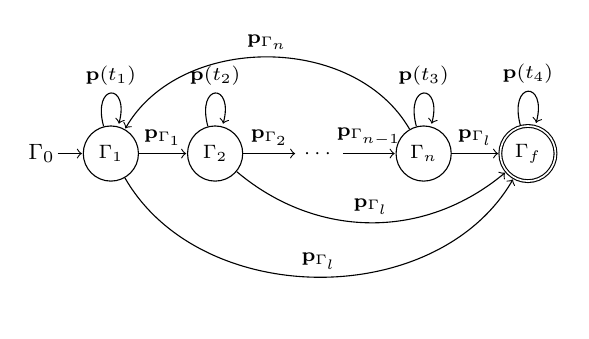
\begin{tikzpicture}[shorten >=.3pt,node distance=12.5ex,on grid,auto,initial text=\hspace*{-.8ex}\footnotesize{$\Gamma_0$}\hspace*{-.5ex}]
      \scriptsize
      \node[state,initial] (q_i) {$\Gamma_1$}; 
      \node[state] (q_2) [right=of q_i] {$\Gamma_2$}; 
      \node        [right=of q_2] (q_dots0) {$\cdots$};
      \node[state] (q_0) [right=of q_dots0] {$\Gamma_n$};
      \node[state,accepting] (q_f) [right=of q_0] {$\Gamma_f$};
      \path[->]
      (q_i) edge node {$\mathbf{p}_{\Gamma_{1}}$} (q_2)
      (q_2) edge node {$\mathbf{p}_{\Gamma_{2}}$} (q_dots0)
      (q_dots0) edge node{$\mathbf{p}_{\Gamma_{n-1}}$} (q_0)
      (q_0) edge [bend right=60] node [above] {$\mathbf{p}_{\Gamma_n}$} (q_i)
      (q_i) edge [bend left=-60] node [above] {$\mathbf{p}_{\Gamma_l}$} (q_f)
      (q_2) edge [bend left=-40] node [above] {$\mathbf{p}_{\Gamma_l}$} (q_f)
      (q_0) edge node {$\mathbf{p}_{\Gamma_{l}}$} (q_f)    
      (q_i) edge [loop above] node {$\mathbf{p}(t_1)$} (q_i)
      (q_2) edge [loop above] node {$\mathbf{p}(t_2)$} (q_2)
      (q_0) edge [loop above] node {$\mathbf{p}(t_3)$} (q_0)
      (q_f) edge [loop above] node {$\mathbf{p}(t_4)$} (q_f)
      ; %end path 
      %\draw [decorate,decoration={brace,amplitude=10pt,mirror,raise=47pt},yshift=0pt]
      %(q_i.south west) -- (q_f.south west) node [black,midway,yshift=-19ex]{$\Gamma$};
    \end{tikzpicture}
  \end{minipage}\hfill
  \begin{minipage}[c]{0.18\columnwidth}
    \centering
    \caption{Plan $\Gamma$ with $n$ primitive stages in Def.~\ref{def:primitive}.}
    \label{fig:state-machine-loop}
  \end{minipage}
  \vspace*{-4ex}
\end{figure}
%\begin{figure}[h!]
%  \center
%  \vspace*{-2.2ex}
%  \begin{tikzpicture}[shorten >=.5pt,node distance=12.5ex,on grid,auto,initial text=\hspace*{-3ex}\footnotesize{$\Gamma_0$}]
%    \scriptsize
%    \node[state,initial] (q_i) {$\Gamma_1$}; 
%    \node[state] (q_2) [right=of q_i] {$\Gamma_2$}; 
%    \node        [right=of q_2] (q_dots0) {$\cdots$};
%    \node[state] (q_0) [right=of q_dots0] {$\Gamma_n$};
%    \node[state,accepting] (q_f) [right=of q_0] {$\Gamma_f$};
%    \path[->]
%    (q_i) edge node {$\mathbf{p}_{\Gamma_{1}}$} (q_2)
%    (q_2) edge node {$\mathbf{p}_{\Gamma_{2}}$} (q_dots0)
%    (q_dots0) edge node{$\mathbf{p}_{\Gamma_{n-1}}$} (q_0)
%    (q_0) edge [bend right=60] node [above] {$\mathbf{p}_{\Gamma_n}$} (q_i)
%    (q_i) edge [bend left=-60] node [above] {$\mathbf{p}_{\Gamma_l}$} (q_f)
%    (q_2) edge [bend left=-40] node [above] {$\mathbf{p}_{\Gamma_l}$} (q_f)
%    (q_0) edge node {$\mathbf{p}_{\Gamma_{l}}$} (q_f)    
%    (q_i) edge [loop above] node {$\mathbf{p}(t_1)$} (q_i)
%    (q_2) edge [loop above] node {$\mathbf{p}(t_2)$} (q_2)
%    (q_0) edge [loop above] node {$\mathbf{p}(t_3)$} (q_0)
%    (q_f) edge [loop above] node {$\mathbf{p}(t_4)$} (q_f)
%    ; %end path 
    %\draw [decorate,decoration={brace,amplitude=10pt,mirror,raise=47pt},yshift=0pt]
    %(q_i.south west) -- (q_f.south west) node [black,midway,yshift=-19ex]{$\Gamma$};
%  \end{tikzpicture}
%  \vspace*{-2.3ex}
%  \caption[Definition of a plan with a loop]{Definition of a plan $\Gamma$ with periodic patterns. Stages $\Gamma_1,\Gamma_2,\dots,\Gamma_n$ containing primitive paths $\varphi_1,\varphi_2,\dots,\varphi_n$ are iterated with a shift $\mathbf{d}$.}
%  \vspace*{-1ex}
%  \label{fig:state-machine-loop}
%\end{figure}

Fig.~\ref{fig:state-machine-loop} illustrates the concept. %s in Definition~\ref{def:primitive}. 
A plan composed of $n$ stages $\Gamma_1,\dots,\Gamma_n$ (%containing 
{\color{blue}with }primitive paths $\varphi_1,\dots,\varphi_n$) is reiterated with the shift $\mathbf{d}$. $t_1<\dots<t_4$ are time instants $\in\mathbb{R}_{> 0}$. $\Gamma_f$ is the accepting stage, indicating the plan is complete, $\Gamma_0$ the initial stage where the aerial robot awaits the starting command.

\vspace*{-.7ex}
\subsection{Energy-aware planning-scheduling problem}
\label{sec:pbfor}

The problem %of planning-scheduling 
is {\color{blue}split into }%composed of 
%two%sub-problems.
{\color{blue}the derivation }%. One is 
%to form a %static 
{\color{blue} of} a {\color{blue}coverage} plan %that visits every point in space 
{\color{blue}and its} {\color{blue}energy-aware} %other to
re-plan{\color{blue}ing}~and~-schedul{\color{blue}ing~}%the plan 
in-flight.~The %in an energy-aware way. %{\color{blue}, whereas }
{\color{blue} 
re-planning-scheduling improves a performance metric--%, which is %quality of the plan and schedule against battery state of charge (SoC), i.e., the 
the weighted average of parameters divided by the remaining battery state of charge (SoC), both in percent (e.g., $\underline{c}_{i,j}$, $\overline{c}_{i,j}$ correspond to 0 and 100). The objective is~%then 
high~average~parame- ters configuration and battery usage with successful %area 
coverage.
%The performance metric the re-planning-scheduling %in the letter 
%improves is %then
%the quality of the plan-schedule against battery state of charge (SoC), e.g., weighted average value of parameters divided by remaining %battery 
%SoC.% at the end of the flight.
}\vspace*{-2.7ex}

\begin{pb}[Coverage and re-planning-scheduling problem]
  \label{pb:cov-pb}
  Consider a finite set of vertices of a polygon $v:=\{v_1,v_2,\dots\}$ where each %vertex $v_i:=(x_{v_i},y_{v_i})%,\forall i\in[|v|]_{>0}$
  %,\,o_{j,k}:=(x_{o_{j,k}},y_{o_{j,k}}),\,\forall j\in|o|,k\in|o_j|$ 
  is a point w.r.t. $\mathcal{O}_W$. 
  Let $\underline{r}\in\mathbb{R}_{\geq 0}$, the vehicle's turning radius, and $\mathbf{p}(t_0)$, the starting point at the time instant $t_0$, be given. 
  The \emph{coverage problem} is the problem of finding a plan $\Gamma$ to cover the polygon, whereas the \emph{re-planning-scheduling problem} is finding the {\color{blue}energy-aware} trajectory of parameters $c_i$ in time{\color{blue}, optimizing battery SoC}.
\end{pb}    

%, i.e, $|\mathbb{X}|:=\sum_{x\in\mathbb{X}}1$
%.

%\begin{pb}[Re-planning-scheduling problem]
%  \label{pb}
%  Consider an initial plan $\Gamma$ in Definition~\ref{def:plan}. The \emph{re-planning-scheduling problem} is the problem of finding the optimal configuration of path and computations parameters $c_i(t),\,\forall i\in\{1,2,\dots\}$ under energy constraints and uncertainty at each time step $t$.
%\end{pb}

Here, $c_i$ denotes a row vector with both the path and computation parameters in sequence, i.e., $c_i:=[\begin{matrix}\,c_i^\rho & c_i^\sigma\,\end{matrix}]'$. %The notation .


%The algorithm inputs a user-specified initial plan that consist of different stages. At each stage the plan contains some parameters that allow to alter the path and computations along an energy budget. The alterations are bounded. There is one path constraint set which bounds the path and multiple computation constraint sets, one per each computation parameter, that bound computations. In Fig.~\ref{fig:il-abs}, there are two parameters. One relative to the path (\ref{sth:ii}~has a shorter distance between the lines than~\ref{sth:iii}), and the other one to the computations (\ref{sth:i}~processes more images per second than~\ref{sth:ii}). 

%The algorithm outputs the control (the parameters) using model predictive control (MPC)~\cite{rawlings2017model} where it checks the satisfaction of the battery constraints. The control is data-driven. Energy sensor data estimates some coefficients of an energy model used to predict future energy consumption in presence of uncertainty. The energy budget is the battery capacity and other battery parameters. These are fixed values that are not replanned by the algorithm. Our goal is to complete the plan with the highest possible parameters configuration as the UAV flies and its batteries drain. 

%\subsection{Plan definition}
%\label{sec:prelim}

%Let us adopt the following mathematical notation. Given an integer $a$, $[a]$ is the set $\{0,1,\dots,a\}$, $[a]^+$ the set $[a]/\{0\}$. Bold lower-case letters indicates vectors. $c_{i,j}$ the $j$-th parameter of the $i$-th parameters set $c_i$. $\underline{c}_{i,j},\overline{c}_{i,j}$ are the lower and upper bounds of the parameter $c_{i,j}$.

%Let us assume that the path at stage $i$ can be altered with $\rho$ path parameters $c_i^\rho:=\{c_{i,1},c_{i,2},\dots,c_{i,\rho}\}$, and the computations with $\sigma$ computation parameters $c_i^\sigma:=\{c_{i,\rho+1},c_{i,\rho+2},\dots,c_{i,\rho+\sigma}\}$. We then express the path as a continuous twice differentiable function $\varphi_i:\mathbb{R}^2\times\mathbb{R}^\rho\rightarrow\mathbb{R}$ of a point and the path parameters. The function returns a metric of the distance between the point and the nominal trajectory. We express the computations as the value of the computation parameters. We discuss the concrete meaning of the value of path parameters in Subsection~\ref{sec:model}, and computation parameters in Subsection~\ref{sec:computations-model}.

%\begin{defn}[Stage, plan, triggering, and final point]\label{def:mission}
%  The $i$-th \emph{stage} $\Gamma_i$ at time instant $k$ of a plan $\Gamma$ is defined
%  \begin{equation*}\begin{split}
%    \Gamma_i:=\{\varphi_i(\mathbf{p}_k,c_i^\rho),c_i^\sigma\mid
%    \,&\exists\,\,\mathbf{p}_k,\,\varphi_i(\mathbf{p}_k,c_i^\rho)\in\mathcal{C}_i,\,\\
%      &\,\forall j\in[\sigma]^+,\,c_{i,\rho+j}\in\mathcal{S}_{i,j}\,\},
%\end{split}\end{equation*}
%where $\mathcal{C}_i:=[\underline{c}_i,\overline{c}_i]\subseteq\mathbb{R}$ is the path constraint set, and $\mathcal{S}_{i,j}:=[\underline{c}_{i,\rho+j},\overline{c}_{i,\rho+j}]\subseteq\mathbb{Z}_{\geq 0}$ the $j$-th computation constraint set. $\mathbf{p}_k$ is a point of a UAV flying at an altitude $h\in\mathbb{R}_{>0}$
%\footnote{The altitude might change at different flying phases and under different atmospheric conditions}
%w.r.t. some inertial navigation frame $\mathcal{O}_W$.   
  
%In Fig.~\ref{fig:traj1}, $\varphi_1,\dots,\varphi_6$ are paths. $\varphi_1$ and $\varphi_5$ are circles, while $\varphi_2$, $\varphi_4$, and $\varphi_6$ are lines. They are all relative to different stages $\Gamma_1,\Gamma_2,\dots$. The constraints set $\mathcal{C}_1,\mathcal{C}_2,\dots$ forms the area where the paths $\varphi_1,\varphi_2,\dots$ can be altered with the parameters $c_{i,1},\dots,c_{i,\rho}$ (gray area in the figure). This area is bounded by $\underline{c}_i,\overline{c}_i$, and can be different per each stage (in Fig.~\ref{fig:traj1}, the area relative to $\Gamma_4$ is bounded by $\underline{c}_4,\overline{c}_4$).

%The \emph{plan} is a finite state machine (FSM) $\Gamma$ where the state-transition function $s:\bigcup_i{\Gamma_i}\times\mathbb{R}^2\rightarrow\bigcup_i{\Gamma_i}$ maps a stage and a point to the next stage
%\begin{equation*}s(\Gamma_i,\mathbf{p}_k):=\begin{cases}
%  \Gamma_{i+1} & \text{if }\mathbf{p}_k=\mathbf{p}_{\Gamma_i}\\
%  \Gamma_i & \text{otherwise}
%\end{cases}.\end{equation*}
%The point $\mathbf{p}_{\Gamma_{i}}$ that allows the transition between $\Gamma_i$ and $\Gamma_{i+1}$ is called \emph{triggering point}. In Fig.~\ref{fig:traj1}, $\mathbf{p}_{\Gamma_1}$ allows the transition between $\Gamma_1$ and $\Gamma_2$, $\mathbf{p}_{\Gamma_4}$ between $\Gamma_4$ and $\Gamma_5$, and $\mathbf{p}_{\Gamma_5}$ between $\Gamma_5$ and $\Gamma_6$. The last triggering point $\mathbf{p}_{\Gamma_{l}}$ relative to the last stage $\Gamma_l$ is called \emph{final point}.
%\end{defn}

%\begin{figure}[h]
%  \center
%  \begin{tikzpicture}[shorten >=.5pt,node distance=10.5ex,on grid,auto]
%    \footnotesize
%    \node[state,initial] (q_i) {$\Gamma_1$}; 
%    \node        [right=of q_i] (q_dots0) {$\cdots$};
%    \node[state] (q_0) [right=of q_dots0] {$\Gamma_i$};
%    \node        (q_dots1) [right=of q_0] {$\cdots$};
%    \node[state,accepting] (q_f) [right=of q_dots1] {$\Gamma_f$};
%    \path[->]
%    (q_i) edge node {$\mathbf{p}_{\Gamma_{1}}$} (q_dots0)
%    (q_dots0) edge node{$\mathbf{p}_{\Gamma_{i-1}}$} (q_0)
%    (q_0) edge node {$\mathbf{p}_{\Gamma_i}$} (q_dots1)
%    (q_dots1) edge node {$\mathbf{p}_{\Gamma_{l}}$} (q_f)    
%    (q_i) edge [loop above] node {$\mathbf{p}_{k_1}$} (q_i)
%    (q_0) edge [loop above] node {$\mathbf{p}_{k_2}$} (q_0)
%    (q_f) edge [loop above] node {$\mathbf{p}_{k_3}$} (q_f)
%    ; %end path 
%    \draw [decorate,decoration={brace,amplitude=10pt,mirror,raise=10pt},yshift=0pt]
%    (q_i.south west) -- (q_f.south west) node [black,midway,yshift=-9ex]{$\Gamma$};
%  \end{tikzpicture}
%  \caption{The plan defined as a FSM}
%  \label{fig:state-machine}
%\end{figure}

%A slice of the plan in Fig.~\ref{fig:state-machine} shows the transition between the stages with the FSM. The triggering point $\mathbf{p}_{\Gamma_{i-1}}$ allows the transition to the stage $\Gamma_i$. The UAV remains in the stage with any generic point $\mathbf{p}_{k_2}$. It eventually enters the stage $\Gamma_{i+1}$ with the triggering point $\mathbf{p}_{\Gamma_i}$ and so on, until it reaches the final point. The stage $\Gamma_f$ is the accepting stage (it indicates that the UAV has completed the plan).

%\begin{figure}[h]
%  \center
%  \begin{tikzpicture}[shorten >=1pt,node distance=23ex,on grid,auto] 
%    \node        (q_dots0) {$\cdots$};
%    \node[state] (q_0) [right=of q_dots0] {$\Gamma_i$};
%    \node        (q_dots1) [right=of q_0] {$\cdots$};   
%    \path[->]
%    (q_dots0) edge node{$\mathbf{p}_{\Gamma_{i-1}}(c_1^\rho,\dots,c_{i-1}^\rho)$} (q_0)
%    (q_0) edge node {$\mathbf{p}_{\Gamma_i}(c_1^\rho,\dots,c_{i}^\rho)$} (q_dots1)    
%    (q_0) edge [loop above] node {$\mathbf{p}_{k}$} (q_0)
%    ; %end path
%  \end{tikzpicture}
%  \caption{Detail of the stage $\Gamma_i$ in the FSM}
%  \label{fig:state-machine2}
%\end{figure}

%Generally, one can express the triggering points in function of the $i$-th trajectory parameters $c_{i}^{\rho}$, or any previous trajectory parameters, propagating the information therein if necessary (see Fig.~\ref{fig:state-machine2}).

%We refer the reader to an example in Appendix~\ref{app:plan-example} for a detailed implementation. In the example, the first trajectory parameter is propagated to all the following trajectories and triggering points. 

%We store the initial plan in the plan specification, the format is described in Appendix~\ref{app:plan-spec}. 

%\subsection{Problem formulation}

%In order to simplify the problem formulation, we consider some primitive paths. All the other paths are built from these paths with a shift $\mathbf{d}:=(x_d,y_d)$.

%Given $n\in\mathbb{Z}_{>0}$ ($n<l,l/n\in\mathbb{Z}$) primitive paths $\varphi_1,\dots\varphi_n$, a generic starting point $\mathbf{p}$ and the current levels of the path parameters $c_1^\rho$, all the other paths $\varphi_{n+1},\dots,\varphi_l$ are built
%\begin{equation}\label{eq:primitive}\begin{split}
%  &\varphi_{(i-1)n+j}(\mathbf{p}+(i-1)\mathbf{d},c_1^\rho)-\\ &\,\,\,\varphi_{in+j}(\mathbf{p}+i\mathbf{d},c_1^\rho)=e_j,
%\end{split}\end{equation}
%$\forall i\in[l/n-1]^+,j\in[n]^+$, where $e_j\in\mathbb{R}$ is the $j$-th constant difference.

%\begin{defn}[Period]\label{def:period}
%  The period $T\in\mathbb{R}_{> 0}$ is the time between $\varphi_{(i-1)n+j}$ and $\varphi_{in+j}$ in Eq.~(\ref{eq:primitive}).
%\end{defn} 

%The algorithm measures the time between the paths and assumes the initial period is one. The periods might be different for different $j$s due to atmospheric interferences.

%One can define the plan using primitive paths or define all the stages explicitly and find $n$ searching the value which satisfies the Eq.~(\ref{eq:primitive}). If there is no such value, (e.g., when the plan is composed of only one stage), the period $T$ from Definition~\ref{def:period} can be determined empirically from energy data (such as these shown in Fig.~\ref{fig:il-abs}).

%\begin{pb}[UAV planning problem]\label{pb}
%  Consider an initial plan $\Gamma$ from Definition~\ref{def:mission}. We are interested in the planning of the parameters $c_i,\,\forall i\in[l]^+$ and energy constraints and in the guidance of the UAV to the path resulting from such plan.
%\end{pb}


%%%%%%%%%%%%%%%%%%%%%%%%%%
\section{Energy Models}  %
\label{sec:energy-model} %
                         %
The solution to the problem requires energy models, predicting the impact of changes to path and computation parameters on the battery. %at future time instants. To this end, 
Sections~\ref{sec:mod-mot}--\hyperref[sec:mod-bat]{C} provide models for the overall and computations energies {\color{blue}and }%as well as 
battery evolution.

\subsection{Overall energy model% for the motion
}
\label{sec:mod-mot}

The collected energy data and corresponding spectrum analysis in Fig.~\ref{fig:il-abs} show the energy of a static coverage plan. It is relative to one flight of a series of flights for CPP exhibiting periodic behavior in a precision agriculture use case~\cite{seewald2020mechanical}. %$\Gamma$ with four primitive path functions iterated with a shift. 
Assuming the primitive paths have approximately the same length and the aerial robot has a fixed ground speed, the data exhibits periodic behavior with a constant set of frequencies, independent of the shift. The hypothesis is further backed by the power spectrum analysis, indicating that to model the energy, three frequencies are adequate.

%We refer to the instantaneous energy consumption evolution simply as the energy signal. We model the energy using energy coefficients $\mathbf{q}\in\mathbb{R}^m$ that characterize such energy signal. The coefficients are derived from Fourier analysis (the size of the energy coefficients vector $m$ is related to the order of a Fourier series) and estimated using a state estimator. %(Kalman filter); well, potentially here with simulated data one could use other estimators (least square filter would work I bet) 

%We prove a relation between the energy signal and the energy coefficients in Lem.~\ref{lem:eqv}. We show after the main results how this approach allows us variability in terms of non-periodic signals.

%After having illustrated the energy model, we enhance it with the energy contribution of the path in Subsection~\ref{sec:model}, and of the computations in Subsection~\ref{sec:computations-model}. 

An intuitive way of modeling the energy data is a Fourier series of a given order $r\in\mathbb{Z}_{\geq 0}$ and period $T\in\mathbb{R}_{>0}$
\begin{equation}\label{eq:fourier}
  h(t)=a_0/T+(2/T)\sum_{j=1}^{r}{\left(a_j\cos{\omega jt}+b_j\sin{\omega jt}\right)},
\end{equation}
where $h:\mathbb{R}_{\geq 0}\rightarrow\mathbb{R}$ maps time to the instantaneous energy% consumption
, $\omega:=2\pi/T$ is the angular frequency, and $a,b\in\mathbb{R}$ %the %series 
coefficients.

%The model in 
Equation~(\ref{eq:fourier}) does not account for the variation of parameters, where, e.g., two schedules result in different instantaneous energies.
%The model in Equation~(\ref{eq:fourier}) does not quantify the contribution of path and computations parameters $c_i$, where, e.g., different schedules result in different instantaneous energy. 
For this latter purpose, we use the dynamics %another model
\begin{subequations}\label{eq:state-perf}
  \begin{align}
  \dot{\mathbf{q}}(t)&=A\mathbf{q}(t)+B\mathbf{u}(t),\label{eq:state-perf-q}\\
  y(t)&=C\mathbf{q}(t),\label{eq:state-perf-y}
\end{align}
\end{subequations}
where $y(t)\in\mathbb{R}$ is the instantaneous energy consumption. The state $\mathbf{q}\in\mathbb{R}^m$ with $m:=2r+1$ contains energy coefficients
\begin{equation}
  \mathbf{q}(t)=\begin{bmatrix}
    \alpha_0(t) & \alpha_1(t) & \beta_1(t) & \cdots & \alpha_r(t) & \beta_r(t)
  \end{bmatrix}'.
\end{equation}

The state transition matrix
\begin{equation}\label{eq:mat_A}{\small
  A=\begin{bmatrix}
    0            & 0^{1\times 2}& \dots & 0^{1\times 2} \\
    0^{2\times 1}& A_1          & \dots & 0^{2\times 2} \\
    \vdots       & \vdots       & \ddots& \vdots        \\
    0^{2\times 1}& 0^{2\times 2}& \dots & A_r 
  \end{bmatrix},\,\,A_j:=\begin{bmatrix}0 & \omega j \\ -\omega j & 0\end{bmatrix}},
\end{equation}
where $A\in\mathbb{R}^{m\times m}$ contains $r$ sub-matrices $A_j$ and $0^{i\times j}$ is a zero matrix of $i$ rows and $j$ columns. In matrix $A$, the top left entry is zero, the diagonal entries are $A_1,\dots,A_r$, the remaining entries are zeros.

The output matrix\vspace*{-3ex}
\begin{equation}\label{eq:mat_C}
  C=(1/T)\Big[1 \,\,\, \overbrace{\begin{matrix}1 & 0 &\cdots & 1 & 0\end{matrix}}^{2r}\Big],
\end{equation}
where $C\in\mathbb{R}^m$ (the first value in the first column is one, the pattern one--zero is then repeated $2r$ times).


%\begin{equation}\label{eq:state-details}\begin{split}
%  A&=\left[\begin{array}{cccc}
%    0&                     &       & \makebox(-5,-5){*}  \\
%     & A_1                 &       &  \\
%     & \makebox(-25,-15){*}& \ddots&  \\
%     &                     &       & A_r 
%  \end{array}\right],\,A_j:=\begin{bmatrix}0 & \omega j \\ -\omega j & 0\end{bmatrix},\\
%  C&=(1/T)\left[\begin{array}{cccccc}
%    1 & 1 & 0 &\cdots & 1 & 0
%  \end{array}\right],
%\end{split}\end{equation}
%where $\mathbf{q}\in\mathbb{R}^m$ with $m=2r+1$, $A\in\mathbb{R}^{m\times m}$ is the state transition matrix, and $C\in\mathbb{R}^m$ is the output matrix. In matrix $A$, the top left entry is zero, the diagonal entries are $A_1,\dots,A_r$, the remaining entries are zeros (*).

%The linear model in Eq.~(\ref{eq:state-perf}) allows us to include the control in the model of Eq.~(\ref{eq:fourier}).

To define the nominal control and the output matrix, we exploit the effect of variation of path and computation parameters on the energy. 
%We assume a variation in computations parameters $c_i^\sigma$ affects the instantaneous energy, i.e., different schedules of power-demanding computational tasks have different power drains from the computing hardware.
%\begin{lem}[Parameters, energy relation]\label{lem:new}
  Given $c_i(t)$ parameters at two following time instants $t\in\{t_j,t_{j+1}\}\subset\mathbb{R}_{\geq 0}$ s.t. $t_j<t_{j+1}$ for an arbitrary stage $\Gamma_i$, a change in parameters $c_i(t_j)\neq c_i(t_{j+1})$ results in different overall and instantaneous energies for path and computation parameters respectively.
%\end{lem}

%Apps.~\ref{app:proof-eqv}--\ref{app:proof-new} contain the proofs of Lemmas~\ref{lem:eqv}--\hyperref[lem:new]{2}.

%Using the same notation from Lem.~\ref{lem:new}, 
%
%\begin{equation}\label{eq:nom-cont}
%  \mathbf{u}(t_{j+1}):=\hat{\mathbf{u}}(t_{j+1})-\hat{\mathbf{u}}(t_j),
%\end{equation}
%for all time instants. 
The nominal control and input matrix in Eq.~(\ref{eq:state-perf}) simply includes the change in energy for all time instants, i.e.,
\begin{equation}\label{eq:mat_B}{\small
  \mathbf{u}(t_{j+1})\hspace*{-.5ex}:=\hspace*{-.5ex}\hat{\mathbf{u}}(t_{j+1})\hspace*{-.5ex}-\hspace*{-.5ex}\hat{\mathbf{u}}(t_j),\,\,\,B=\begin{bmatrix}
      0^{1\times\rho} & 1      & \cdots & 1      \\
      0^{1\times\rho} & 0      & \cdots & 0      \\ 
      \vdots          & \vdots & \ddots & \vdots \\
      0^{1\times\rho} & 0      & \cdots & 0   
  \end{bmatrix}},
\end{equation}
shifts the base frequency $\alpha_0$ assuming the energy of the computations does not alter the other frequencies. $B\in\mathbb{R}^{m\times n}$ with $n:=\rho+\sigma$ contains zeros but in the first row where the first $\rho$ columns are zeros and the remaining $\sigma$ are ones. Different combinations of $\mathbf{u}$ with matrix $B$ in Eq.~(\ref{eq:mat_B}) are possible %, as we discuss briefly in 
{\color{blue}(see }Section~\ref{sec:conclusion}{\color{blue})}.
The dynamics in Eqs.~(\ref{eq:state-perf}--\ref{eq:mat_B}) additionally allows us to use state estimation techniques, such as the Kalman filter in Section~\ref{sec:repla-algo}, to refine the states $\mathbf{q}$ and model the energy of the aerial robot flying under diverse %atmospheric 
conditions.

{\color{blue}Matrices $A$ and $C$ are constructed such that t}he %Under favorable conditions, %the 
models in Eqs.~(\ref{eq:fourier}--\ref{eq:state-perf}) are equal
%\begin{lem}[Signal, output equality]\label{lem:eqv}Given 
when $\mathbf{u}$ is a zero vector %, matrices $A,C$ described by Eqs.~(\ref{eq:mat_A}--\ref{eq:mat_C}), 
and an initial guess $\mathbf{q}(t_0)=\mathbf{q}_0$ at initial time instant $t_0$
  {\color{blue}\begin{equation}
  {\color{black}\mathbf{q}_0=\begin{bmatrix}a_0 & a_1/2 & b_1/2 & \cdots & a_r/2 & b_r/2\end{bmatrix}',}
  \end{equation}}
  %$h$ in Eq.~(\ref{eq:fourier}) is equal to $y$ in Eq.~(\ref{eq:state-perf}).
%\end{lem}
%\begin{proof}
%The equality of the signal and output is achieved by a proper choice of the items of matrices $A,C$ and the initial guess $\mathbf{q}_0$. We refer the reader to Appendix~\ref{app:proof-eqv} for a formal proof, where we justify the choices of the items of the matrices and of the initial guess. 
%\end{proof}
%Appendix~\ref{app:proof-eqv} contains a proof of Lem.~\ref{lem:eqv}.
i.e., $h,y$ are %both 
harmonic signals with the same frequencies{\color{blue}. For further details see the first author's Ph.D. thesis~\cite{seewaldphdthesis}}.

$\hat{\mathbf{u}}$ in Eq.~(\ref{eq:mat_B}) is then a scale transformation
\begin{equation}
  \hat{\mathbf{u}}(t):=\mathrm{diag}(\nu_i)c_i(t)+\tau_i,
\end{equation}
where $\mathrm{diag}(x)$ is a diagonal matrix with items of a set $x$ on the diagonal and zeros elsewhere. $\nu_i:=\begin{bmatrix}\nu_{i,1}&\cdots&\nu_{i,n}\end{bmatrix}'$ and $\tau_i:=\begin{bmatrix}\tau_{i,1}&\cdots&\tau_{i,n}\end{bmatrix}'$ are scaling factors{\color{blue},} %that 
transform{\color{blue}ing} parameters %domain 
(see Definition~\ref{def:stage}) to time and power domains.

%For ease of notation, 
{\color{blue}W}e assume that the coverage time evolves linearly{ \color{blue}and that the }path parameters{ \color{blue}contribute to it equally.} $c_i^\rho$ can be {\color{blue}then} transformed into a time measure with scaling factors\begin{subequations}\label{eq:scale-traj}\begin{align}
  \nu_{i,j}&=\left((\overline{t}-\underline{t})/(\overline{c}_{i,j}-\underline{c}_{i,j})\right)/\rho,\\
  \tau_{i,j}&=\left(\underline{c}_{i,j}(\underline{t}-\overline{t})/(\overline{c}_{i,j}-\underline{c}_{i,j})+\underline{t}\right)/\rho,
\end{align}\end{subequations} 
$\forall j\in[\rho]_{>0}$ where $\overline{t},\underline{t}$ are time measures needed to complete the coverage with configurations $\underline{c}_i^\rho,\overline{c}_i^\rho$ ($\underline{\Gamma},\overline{\Gamma}$).

Similarly to Eq.~(\ref{eq:scale-traj}), computation parameters $c_i^\sigma$ can be transformed into an instantaneous energy measure with %scaling factors
\begin{subequations}\label{eq:scale-comp}\begin{align}
  \nu_{i,j}&=(g(\overline{c}_{i,j})-g(\underline{c}_{i,j}))/(\overline{c}_{i,j}-\underline{c}_{i,j}),\\
  \tau_{i,j}&=\underline{c}_{i,j}(g(\underline{c}_{i,j})-g(\overline{c}_{i,j}))/(\overline{c}_{i,j}-\underline{c}_{i,j})+g(\underline{c}_{i,j}),
\end{align}\end{subequations}
$\forall j\in[\rho+1,n]$. The function $g$ is detailed in Section~\ref{sec:mod-com} and quantifies the power of the computing hardware.

\subsection{Energy model for the computations}
\label{sec:mod-com}

Models for heterogeneous computing hardware in the literature often rely on analytical expressions~\cite{marowka2017energy,%goraczko2008energy%calore2015energy,
yang2017designing} or different techniques, such as regressional analysis~\cite{bailey2014adaptive,ma2012holistic,seewald2019coarse}, aiding the selection of hardware- or software-specific parameters. This section presents an energy model based on our early studies~\cite{seewald2019component,seewald2019coarse}, which relies on regressional analysis to quantify the computations energy of any configuration of computations $c_i^\sigma$ within the bounds (see Definition~\ref{def:stage}).

The model compromises an automatic modeling and profiling tool~\cite{seewald2019coarse} named \powprof{} distributed %~\cite{powprofiler} 
under the open-source MIT license. It is segmented into two layers. In the \emph{measurement layer}, the tool measures a discrete set of computation parameters and infers the energy of the remaining in the \emph{predictive layer} via a piecewise linear regression.

We assume there is at least one measuring device, i.e., shunt or internal power resistor, multimeter, or amperemeter, quantifying the power drain of a specific component, e.g., CPU, GPU, memory, etc., or of the entire computing hardware.

\begin{defn}[Measurement layer]\label{def:meas}
  Given a measuring device, computation parameters, and initial and final time instants, the \emph{measurement layer} is the function $\gamma:\mathbb{Z}_{>0}\times\mathbb{Z}^\sigma\times\mathcal{T}\rightarrow\mathbb{R}$ that returns an energy measure.
\end{defn}

Here, the notation $\mathcal{T}$ encloses all the time intervals from initial $t_0$ to final $t_f$, i.e., $\mathcal{T}:=[t_0,t_f]$.

\begin{defn}[Predictive layer]\label{def:pred}
  Given a measuring device and computation parameters, the \emph{predictive layer} is the function $g:\mathbb{Z}_{>0}\times\mathbb{Z}^\sigma\rightarrow\mathbb{R}$ that returns an energy measure.
\end{defn}

The energy measures in Definitions~\ref{def:meas}--\hyperref[def:pred]{2} can be either average expressed in watts or overall expressed in joules. Additionally, the \powprof{} tool supports the battery SoC detailed in Section~\ref{sec:mod-bat}. The function $g$ in Definition~\ref{def:pred} is contained in the %computations scaling 
factors in Eq.~(\ref{eq:scale-comp}), assuming the computations energy behaves linearly between $\underline{c}_i^\sigma$ and $\overline{c}_i^\sigma$, otherwise
\begin{equation}\label{eq:piece-wise-reg}\begin{split}
  g(c_i^\sigma)=(&\gamma(\lceil c_i^\sigma\rceil,\mathcal{T}_1)-\gamma(\lfloor c_i^\sigma\rfloor,\mathcal{T}_2))\\(&c_i^\sigma-\lfloor c_i^\sigma\rfloor)/(\lceil c_i^\sigma\rceil-\lfloor c_i^\sigma\rfloor)+\gamma(\lfloor c_i^\sigma\rfloor,\mathcal{T}_2),
\end{split}\end{equation}
where notation $\lceil c_i^\sigma\rceil,\lfloor c_i^\sigma\rfloor$ indicates two adjacent measurement layers, and $\mathcal{T}_1,\mathcal{T}_2$ are the corresponding two time intervals. {\color{blue}M}easuring device in $\gamma$ and $g$ is {\color{blue}not explicitly stated in Eq.~(\ref{eq:piece-wise-reg})}.

\vspace*{-1.4ex}
\subsection{Battery model}
\label{sec:mod-bat}

The battery model predicts the battery SoC in the function of a given load at future time 
instants. There are multiple models in the literature~\cite{rao2003battery} with varying complexity {\color{blue}and} accuracy %, and ease of implementation 
ranging from accurate but costly physical models~\cite{%moura2017battery,
marcicki2013design}, to abstract models~\cite{%xing2014state,
%he2011evaluation,
hinz2019comparison,mousavi2014various} %that have
{\color{blue}with} compelling trade-offs in terms of the latter two. 
We model a Li-ion battery %of an aerial robot 
in-flight with an abstract ``Rint'' ECM in the literature~\cite{%he2011evaluation,
hinz2019comparison,mousavi2014various}.

The battery SoC changes according to~\cite{hasan2018exogenous%,zhang2018online
}, i.e.,
\begin{equation}\label{eq:batdyn}
  \dot{b}(y(t))=-k_bI(y(t))/Q_c,
\end{equation}
where $I(y(t))\in\mathbb{R}$ is the internal current measured in amperes, $y(t)\in\mathbb{R}_{\geq 0}$ the power drain, and $Q_c\in\mathbb{R}$ the battery constant nominal capacity measured in amperes per hour. $k_b$ is a battery coefficient added to~\cite{hasan2018exogenous%,zhang2018online
} and derived experimentally. The ``Rint'' circuit models the battery as a perfect voltage source connected with a resistor $R_r\in\mathbb{R}$ measured in ohm, representing the battery resistance. The voltage on the extremes of ECM respects $V_e=V-R_rI$, where $V,V_e\in\mathbb{R}$ are the internal and external battery voltages measured in volts. The former can be retrieved from the battery data sheet~\cite{hinz2019comparison} and depends on the SoC~\cite{hasan2018exogenous}.

If the voltage %of the power drain 
is stable, Kirchhoff's circuit laws lead to $V_sI_l=V_eI$, where $I_l$ is the current required by the load %measured 
in amperes. Combining $V_e,V_sI_l$ results in the %quadratic 
expression $R_rI^2-$ $VI+V_sI_l=0$. Solving the expression utilizing the negative solution (when $I_l$ is zero, $I$ should also be zero) %leads to% 
results in 
\begin{equation}\label{eq:batdyn2}
I(y(t))=(V-\sqrt{V^2-4R_ry(t)})/(2R_r).
\end{equation} 
%as in Lem.~\ref{lem:bat}.
%
%\begin{lem}[Battery SoC]\label{lem:bat}
%  Given the internal battery voltage $V\in\mathbb{R}$ measured in volts, resistance $R_r$ in ohms, constant nominal capacity $Q_c$ in amperes per hour, and 
%thus given a battery coefficient $k_b$, the \emph{battery SoC} evolves
%\begin{equation*}\label{eq:batdyn}
%  \dot{b}(t)=-k_b\left(V-
%  \sqrt{
%    V^2-
%    4R_ry(t)}
%  \right)/(2R_rQ_c).
%\end{equation*}
%\end{lem}

%App.~\ref{app:proof-bat} contains the proof of Lem.~\ref{lem:bat}. 

Eq.~(\ref{eq:state-perf}) states that the output $y$ evolves in $\mathbb{R}$, %conflicting with the the findings in this section. 
yet, aerial robots usually use a battery.
We thus use instead
%\begin{defn}[Output constraint]\label{def:const}
\begin{equation}\label{eq:output-const}
  {\small\mathcal{Y}(t):=\{y\mid y\in[0,b\,Q_cV]\subseteq{\mathbb{R}_{\geq 0}}\},} 
\end{equation}
%the \emph{output constraint}, 
where $b\,Q_cV$, the maximum instantaneous energy %consumption
measured in watts, is derived from Eq.~(\ref{eq:batdyn}--\ref{eq:batdyn2}).
%\end{defn}

%Let us consider for practical reasons the discretized version of the system in Eq.~\ref{eq:state-perf}. 

%Let us suppose that at time instant $k$ the plan reached the $i$-th stage $\Gamma_i$ and the control
%\begin{equation}\label{eq:state-control2}
%  \mathbf{u}_k=\begin{bmatrix}c_k^\rho & c_k^\sigma\end{bmatrix}^T,
%\end{equation}
%where $\mathbf{u}_k\in\mathbb{R}^n$ with $n=\rho+\sigma$ differs from the nominal control $\mathbf{u}$ in Eq.~(\ref{eq:state-perf}). We include the control in the nominal control exploiting the following observation. 

%We observe that a change in path parameters affects the energy indirectly. It alters the time when the UAV reaches the final point $\mathbf{p}_{\Gamma_l}$. We use this information later in the algorithm to check that the battery discharge time is greater and replan the path parameters accordingly. A change in computation parameters affects the energy directly. It alters the instantaneous energy consumption as more computations require more power (and vice versa). We replan the computation parameters to maximize the instantaneous energy consumption against the maximum battery discharge rate.

%The nominal control and the input matrix
%\begin{equation}\label{eq:state-control}\begin{split}
%  \mathbf{u}&=(\hat{\mathbf{u}}_k-\hat{\mathbf{u}}_{k-1}),\,\,\,\hat{\mathbf{u}}_k:=\mathrm{diag}(\nu_i)\mathbf{u}_k+\tau_i,\\
%  B&=\begin{bmatrix} 0 & \cdots & 0 & 1 & \cdots & 1 \\ 
%    & & & \makebox(-15,-3){*} & &\end{bmatrix}.
%\end{split}\end{equation}
%The matrix $B\in\mathbb{R}^{m\times n}$ contains zeros (*) except the first row where the first $\rho$ columns are still zeros and the remaining $\sigma$ are ones. $\hat{\mathbf{u}}_k$ is a scale transformation with $\nu_i=\begin{bmatrix}\nu_i^\rho & \nu_i^\sigma\end{bmatrix}^T$ and $\tau_i=\begin{bmatrix}\tau_i^\rho & \tau_i^\sigma\end{bmatrix}^T$ scaling factors quantifying the contribution to the plan of a given parameter in terms of time for the first $\rho$ parameters, and power for the remaining $\sigma$ (we use the same notation for the path and computation scaling factors as for the parameters). The nominal control $\mathbf{u}$ is then the difference of these contributions of two consecutive controls $\mathbf{u}_{k-1},\mathbf{u}_k$ applied to the system. $B\mathbf{u}$ merely includes the difference in power into the model in Eq.~(\ref{eq:state-perf}).
 
%Indeed an alteration of the path affects the overall flying time (and consequently the energy). An alteration the the computations affects the instantaneous energy consumption.

%We clarify how we derive the factors $\nu_i,\tau_i$ in the next two subsections.

%\subsection{Path parameters energy contribution}
%\label{sec:model}

%Eq.~(\ref{eq:state-control}) accounts for the energy due to the change of parameters $\mathbf{u}_k-\mathbf{u}_{k-1}$. For instance, when the trajectory $\varphi_1$ is a circle (see Fig.~\ref{fig:tee1}), a decrement in the trajectory parameter $c_{1,1}$--the radius of the circle--adds a negative contribution. It thus simulates the lowering of instantaneous energy consumption ($\nu_{1,1}c_{1,1}>\nu_{1,1}c_{1,1}^-$) for a given $\nu_{1,1}$, that is then summed to the first coefficient $\alpha_0$ in Eq.~(\ref{eq:state-details}), shifting the modeled energy.

%The set
%\begin{equation}\label{eq:area}
%  \mathcal{P}_i:=\{\mathbf{p}_k\mid\varphi_i(\mathbf{p}_k,c_{i}^\rho)\in\mathcal{C}_i\},
%\end{equation}
%delimits the area where the $i$-th path $\varphi_i$ is free to evolve using the path parameters $c_i^\rho$ (the gray area in Fig.~\ref{fig:tee1}). $\varphi_i$ is a function of the two coordinates and the path parameters, and is equal to zero when a point $\mathbf{p}_k$ is on the path. Physically, this means the UAV is flying exactly over the nominal trajectory. The path parameters allows to change the path. They are a way to alter the nominal trajectory in the initial plan and thus alter the energy by changing the flying time in the example in Fig.~\ref{fig:il-abs}.
%In fact, the algorithm uses the set from Eq.~(\ref{eq:area}) to find the path parameters such that the plan consisting of flying $\varphi_i$ has the highest energy, while still respecting the constraints. In Fig.~\ref{fig:tee1}, the parameter radius of the circle $c_{1,1}$ is replanned as, e.g., averse atmospheric conditions do not allow to terminate the plan.

%We derive the new position $\mathbf{p}_{k+1}$ computing the vector field $\nabla\varphi_i:=\begin{bmatrix}\partial\varphi_i/\partial x & \partial\varphi_i/\partial y\end{bmatrix}^T$, and the direction to follow in the form of velocity vector~\cite{de2017guidance}
%\begin{equation}\label{eq:pd}
%  \dot{\mathbf{p}}_d(\mathbf{p}_k):=E\nabla\varphi_i-k_e\varphi_i\nabla\varphi_i,\,\,\,E=\begin{bmatrix}
%    0&1\\-1&0
%  \end{bmatrix},
%\end{equation}
%where $E$ specifies the rotation (it influence the tracking direction), and $k_e\in\mathbb{R}_{\geq 0}$ the gain to adjusts the speed of convergence. The direction the velocity vector $\dot{\mathbf{p}}_d$ is pointing at is generally different from the course heading $\dot{\mathbf{p}}$ due to the atmospheric interferences (wind $w\in\mathbb{R}$ in the top of Fig.~\ref{fig:tee1}).

%The scaling factors for the path parameters from Eq.~(\ref{eq:state-control}) are derived empirically. For the example in Fig.~\ref{fig:tee1}, we can obtain the scaling factor $\nu_{1,1}$ measuring the time needed to compute the path with the lowest configuration $\underline{c}_1$, $\underline{t}$ and the highest $\overline{t}$. The variation of the control hence results in an approximate measure of the plans' time variation with factors
%\begin{equation}\label{eq:scale-traj}\begin{split}
%  \nu_{i,j}&=\left((\overline{t}-\underline{t})/(\overline{c}_{i,j}-\underline{c}_{i,j})\right)/\rho,\\
%  \tau_{i,j}&=\left(\underline{c}_{i,j}(\underline{t}-\overline{t})/(\overline{c}_{i,j}-\underline{c}_{i,j})+\underline{t}\right)/\rho,
%\end{split}\end{equation} 
%Whenever the trajectory parameters are not equally distributed, one can define $(y_{\overline{c}_i}-y_{\underline{c}_i})$ as a the highest (and lowest) levels of specific trajectory parameters. 
%$\forall j\in[\rho]^+$. Moreover, let the factors be zero when the parameters set $c_i^\rho=\{\emptyset\}$.

%\subsection{Computation parameters energy contribution}
%\label{sec:computations-model}

%Let us recall from Definition~\ref{def:mission} that the $i$-th stage $\Gamma_i$ of the plan $\Gamma$ contains the computation parameters which characterize the computations. We estimate the energy cost of these computations using \powprof{}, the open-source modeling tool adapted from earlier work on computational energy analysis~\cite{seewald2019coarse, seewald2019component}, and energy estimation of a fixed-wing UAV~\cite{seewald2020mechanical}. 

%For this purpose, we assume the UAV carries an embedded board that runs the computations. Our tool measures the instantaneous energy consumption of a subset of possible computation parameters within the computation constraint sets and builds an energy model: a linear interpolation, one per each computation. 

%The computations are implemented by software components, e.g., Robot Operating System (ROS) nodes in a ROS-based system~\cite{quigley2009ros}. The user implements these nodes such that they change the computational load according to node-specific ROS parameters--the computation parameters. In a generic software component system, the user maps the computational load to the arguments~\cite{seewald2019component}. In both cases, with ROS~\cite{zamanakos2020energy} or with generic software components system~\cite{seewald2019component}, the tool performs automatic modeling. For instance, if the computation is an object detector, a computation parameter $c_{1,2}$ might correspond to frames-per-second (fps) rate. The tool then measures power according to the detection frequency.

%We note that while the path can differ for each stage, the tasks remain the same. However, the user can inhibit or enable a computation varying its computation constraint set.

%Let us define $g:\mathbb{Z}_{\geq 0}\rightarrow\mathbb{R}_{\geq 0}$ as the instantaneous computational energy consumption value obtained using the tool.

%The scaling factors add the computational energy component to the model in Eq.~(\ref{eq:state-perf}). They are derived similarly to Eq.~(\ref{eq:scale-traj})
%\begin{equation*}\begin{split}
%  \nu_{i,j}&=(g(\overline{c}_{i,j})-g(\underline{c}_{i,j}))/(\overline{c}_{i,j}-\underline{c}_{i,j}),\\
%  \tau_{i,j}&=\underline{c}_{i,j}(g(\underline{c}_{i,j})-g(\overline{c}_{i,j}))/(\overline{c}_{i,j}-\underline{c}_{i,j})+g(\underline{c}_{i,j}),
%\end{split}\end{equation*}
%$\forall j\in[\rho+1,\rho+\sigma]$. Moreover, let the factors be zero when the parameters set $c_i^\sigma=\{\emptyset\}$.


\vspace*{-1.4ex}
%%%%%%%%%%%%%%%%%%%%%%%%%%%%%%%%
\section{Planning-Scheduling}  %
\label{sec:algo}               %
                               %
\begin{figure}[t]
  \footnotesize
  \begin{minipage}[l]{0.21\columnwidth}
    \caption{Alteration of the path parameter $c_{i,1}$, the radius of the circle (i.e., the alteration of the plan in Fig.~\ref{fig:il-abs}).
    }
    \label{fig:tee1}
  \end{minipage}\hfill
  \begin{minipage}[c]{0.77\columnwidth}
    \centering
    \vspace*{-4.5ex}
    
\definecolor{cDEDEDE}{RGB}{222,222,222}
\definecolor{c989898}{RGB}{152,152,152}
\definecolor{c2B2B2B}{RGB}{43,43,43}
\definecolor{cFFFFFF}{RGB}{255,255,255}
\definecolor{c4D4D4D}{RGB}{77,77,77}
\definecolor{c9B9B9B}{RGB}{155,155,155}
\definecolor{c0000FF}{RGB}{0,0,255}
\definecolor{c00FFFF}{RGB}{0,255,255}


\def \globalscale {.870000}
\begin{tikzpicture}[y=0.80pt, x=0.80pt, yscale=-\globalscale, xscale=\globalscale, inner sep=0pt, outer sep=0pt]
  \path[fill=cDEDEDE,line join=round,even odd rule,line width=0.160pt] (224.1960,21.4445) .. controls (230.8220,19.2249) and (237.6080,17.6786) .. (244.9510,17.5492) -- (244.9510,53.9795) .. controls (227.5490,54.6188) and (213.5140,68.4420) .. (212.5390,85.7558) -- (212.5540,100.1050) -- (212.5390,100.4300) -- (212.5390,100.7590) .. controls (212.5540,101.5870) and (212.6730,102.4470) .. (212.6500,103.2610) -- (212.6570,103.2690) -- (212.6570,105.2820) -- (212.5390,150.8670) -- (212.5390,159.0690) -- (212.5180,159.0690) -- (212.5170,159.2310) -- (212.5050,160.1520) -- (212.5710,164.3450) -- (192.3530,164.3500) .. controls (192.6690,141.5900) and (191.5330,109.2090) .. (192.5090,88.0319) .. controls (192.9850,77.6899) and (195.2800,69.7689) .. (195.9520,67.4317) .. controls (198.4750,58.6611) and (196.6740,32.8197) .. (223.6900,21.6374) -- (224.1960,21.4445) -- cycle;



  \path[draw=c989898,line join=round,line width=0.512pt] (246.1920,87.5565) ellipse (1.9796cm and 1.9796cm);



  \path[draw=black,line join=round,line width=0.512pt] (248.6570,89.8704) -- (243.7920,85.0054);



  \path[draw=c2B2B2B,line join=round,line width=0.512pt] (317.1380,0.4460) -- (317.1370,164.2780);



  \path[draw=black,line join=round,line width=1.024pt] (237.0870,18.3689) .. controls (239.0470,17.5288) and (246.5610,17.5885) .. (246.5610,17.5885) .. controls (285.3010,17.5885) and (316.7060,48.9933) .. (316.7060,87.7328);



  \path[draw=black,line join=round,line width=0.512pt] (243.7930,89.8674) -- (248.6580,85.0029);



    \path[fill=cFFFFFF,line join=round,line width=0.160pt] (324.4000,11.4093) -- (310.2530,11.4093) -- (310.2530,29.5564) -- (324.4060,29.5558) -- (324.4000,11.4093) -- cycle;



    \path[cm={{1.0,0.0,0.0,1.0,(306.0,26.0)}}] (0.0000,0.0000) node[above right] () {VX};



  \path[draw=black,line join=round,line width=1.024pt] (316.7050,164.2910) -- (316.7050,87.5074);



  \path[draw=c2B2B2B,line join=round,line width=0.512pt] (246.8040,87.8051) ellipse (1.5285cm and 1.5285cm);



  \path[draw=c4D4D4D,line join=round,line width=0.512pt] (192.6100,0.3581) -- (192.6090,164.1900);



  \path[draw=black,line join=round,line width=0.512pt] (296.9870,106.9110) -- (246.4180,87.5164);



  \path[draw=black,line join=round,line width=1.024pt] (236.4940,17.9592) .. controls (196.1050,25.4340) and (198.8250,57.4690) .. (195.9570,67.4401) .. controls (192.9930,77.7476) and (192.5410,87.3730) .. (192.5410,87.3730) -- (192.5560,87.6743) -- (192.6030,88.1830);



  \path[draw=black,fill=c9B9B9B,line join=round,line width=0.512pt] (193.0920,79.9088) -- (202.1750,65.7845) -- (196.2420,66.6516) -- (191.7620,63.1692) -- (193.0920,79.9088) -- cycle;



  \path[fill=black,line join=round,line width=0.256pt] (191.9100,153.9330) -- (191.9100,148.6000) -- (193.1900,148.6000) -- (193.1900,153.9330) -- (191.9100,153.9330) -- cycle(191.9100,143.2670) -- (191.9100,137.9330) -- (193.1900,137.9330) -- (193.1900,143.2670) -- (191.9100,143.2670) -- cycle(191.9100,132.6000) -- (191.9100,127.2670) -- (193.1900,127.2670) -- (193.1900,132.6000) -- (191.9100,132.6000) -- cycle(191.9100,121.9330) -- (191.9100,116.6000) -- (193.1900,116.6000) -- (193.1900,121.9330) -- (191.9100,121.9330) -- cycle(191.9100,111.2670) -- (191.9100,105.9330) -- (193.1900,105.9330) -- (193.1900,111.2670) -- (191.9100,111.2670) -- cycle(191.9100,100.6000) -- (191.9100,95.2668) -- (193.1900,95.2668) -- (193.1900,100.6000) -- (191.9100,100.6000) -- cycle(191.9100,89.9334) -- (191.9100,87.8162) -- (193.1900,87.8162) -- (193.1900,89.9334) -- (191.9100,89.9334) -- cycle(191.9100,164.6000) -- (191.9100,159.2670) -- (193.1900,159.2670) -- (193.1900,164.6000) -- (191.9100,164.6000) -- cycle;



    \path[fill=cFFFFFF,line join=round,line width=0.160pt,rounded corners=0.0000cm] (185.7260,11.3214) rectangle (199.8732,29.4686);



    \path[cm={{1.0,0.0,0.0,1.0,(182.0,25.0)}}] (0.0000,0.0000) node[above right] () {VX};



    \path[fill=cFFFFFF,line join=round,line width=0.160pt] (197.3250,158.2760) -- (183.1780,158.2760) -- (183.1390,171.9970) -- (197.3200,171.9620) -- (197.3250,158.2760) -- cycle;



    \path[cm={{1.0,0.0,0.0,1.0,(182.0,170.0)}}] (0.0000,0.0000) node[above right] () {c1};



    \path[fill=cFFFFFF,line join=round,line width=0.160pt,rounded corners=0.0000cm] (257.2650,88.8349) rectangle (281.4121,106.9820);



    \path[cm={{1.0,0.0,0.0,1.0,(259.0,102.0)}}] (0.0000,0.0000) node[above right] () {c
    				2};



  \path[draw=black,fill=cFFFFFF,line join=round,line width=0.512pt] (226.1000,20.6396) -- (242.8690,21.5108) -- (238.4750,17.5101) -- (239.9690,11.1733) -- (226.1000,20.6396) -- cycle;



    \path[fill=cFFFFFF,line join=round,line width=0.160pt] (222.2130,56.6201) -- (204.0660,56.6199) -- (204.0660,74.7670) -- (222.2130,74.7672) -- (222.2130,56.6201) -- cycle;



    \path[cm={{1.0,0.0,0.0,1.0,(206.0,70.0)}}] (0.0000,0.0000) node[above right] () {qk};



    \path[fill=cFFFFFF,line join=round,line width=0.160pt,rounded corners=0.0000cm] (214.1760,2.0732) rectangle (228.3232,16.2204);



    \path[cm={{1.0,0.0,0.0,1.0,(217.0,12.0)}}] (0.0000,0.0000) node[above right] () {p};



  \path[draw=black,line join=round,line width=0.512pt] (226.4700,20.5371) -- (238.3640,17.5090);



  \path[draw=black,line join=round,line width=0.512pt] (193.2910,79.1771) -- (196.1980,66.7255);



    \path[fill=cFFFFFF,line join=round,line width=0.160pt] (244.6550,128.9910) -- (226.5070,128.9920) -- (226.5070,147.1380) -- (244.6550,147.1380) -- (244.6550,128.9910) -- cycle;



    \path[cm={{1.0,0.0,0.0,1.0,(225.0,144.0)}}] (0.0000,0.0000) node[above right] () {VX};



  \path[draw=c989898,line join=round,line width=0.512pt] (176.0540,0.3772) -- (176.0540,164.2100);



  \path[cm={{1.0,0.0,0.0,1.0,(201.0,185.0)}}] (0.0000,0.0000) node[above right] () {(b) path adjustment};



  \path[fill=black,line join=round,line width=0.160pt] (293.9350,102.7120) -- (291.8530,107.6500) -- (297.4170,107.0880) -- (293.9350,102.7120) -- cycle;



  \path[draw=c2B2B2B,line join=round,line width=0.512pt] (152.2510,0.3200) -- (152.2500,164.1520);



    \path[fill=cFFFFFF,line join=round,line width=0.160pt] (158.8140,11.2833) -- (144.6670,11.2833) -- (144.6670,29.4304);



    \path[cm={{1.0,0.0,0.0,1.0,(142.0,26.0)}}] (0.0000,0.0000) node[above right] () {VX};



  \path[fill=cDEDEDE,line join=round,line width=0.160pt] (11.9060,85.0887) -- (11.9343,85.0887) .. controls (12.9880,47.6981) and (43.3023,17.6289) .. (80.7900,16.9684) -- (80.7900,53.3987) .. controls (63.3884,54.0380) and (49.3534,67.8611) .. (48.3783,85.1750) -- (48.3929,99.5239) -- (48.3783,99.8487) -- (48.3783,100.1780) .. controls (48.3936,101.0060) and (48.5128,101.8670) .. (48.4899,102.6800) -- (48.4960,102.6880) -- (48.4960,104.7010) -- (48.3783,150.2860) -- (48.3783,158.4880) -- (48.3571,158.4880) -- (48.3567,158.6500) -- (48.3446,159.5710) -- (48.4105,163.7650) -- (11.7063,163.7730) .. controls (11.7063,161.8710) and (11.6822,165.6310) .. (11.6707,161.4240) -- (11.6707,159.6720) -- (11.6707,159.3160) -- (11.6707,158.8400) -- (11.6707,158.4930) -- (11.6707,87.3190) -- (11.9060,85.0887) -- cycle;



  \path[draw=c2B2B2B,line join=round,line width=0.512pt] (81.7300,87.5399) ellipse (1.9796cm and 1.9796cm);



  \path[draw=black,line join=round,line width=0.512pt] (84.1885,89.8517) -- (79.3297,84.9872);



  \path[draw=black,line join=round,line width=0.512pt] (79.3325,89.8514) -- (84.1975,84.9866);



  \path[draw=c2B2B2B,line join=round,line width=0.512pt] (11.6130,0.3414) -- (11.6123,164.1740);



  \path[draw=black,line join=round,line width=0.512pt] (81.8116,87.4557) -- (11.5289,87.4557);



  \path[fill=black,line join=round,line width=0.160pt] (17.2158,90.0878) -- (17.2088,84.7293) -- (12.3038,87.4145) -- (17.2158,90.0878) -- cycle;



    \path[fill=cFFFFFF,line join=round,line width=0.160pt,rounded corners=0.0000cm] (4.7286,11.3047) rectangle (18.8758,29.4518);



    \path[cm={{1.0,0.0,0.0,1.0,(1.0,26.0)}}] (0.0000,0.0000) node[above right] () {VX};



  \path[draw=black,line join=round,line width=1.024pt] (72.2687,18.1599) .. controls (74.2288,17.3198) and (81.7430,17.3795) .. (81.7430,17.3795) .. controls (120.4830,17.3795) and (151.8870,48.7842) .. (151.8870,87.5239);



    \path[fill=cFFFFFF,line join=round,line width=0.160pt,rounded corners=0.0000cm] (100.3810,14.9448) rectangle (118.5282,29.0920);



    \path[cm={{1.0,0.0,0.0,1.0,(99.0,29.0)}}] (0.0000,0.0000) node[above right] () {VX};



    \path[fill=cFFFFFF,line join=round,line width=0.160pt] (55.4211,158.2770) -- (41.2739,158.2770) -- (41.2532,171.9450) -- (55.4334,171.9450) -- (55.4211,158.2770) -- cycle;



    \path[cm={{1.0,0.0,0.0,1.0,(46.0,170.0)}}] (0.0000,0.0000) node[above right] () {c1};



    \path[fill=cFFFFFF,line join=round,line width=0.160pt] (69.0222,84.4727) -- (48.8751,84.4721) -- (48.8751,98.6193) -- (69.0222,98.6198) -- (69.0222,84.4727) -- cycle;



    \path[cm={{1.0,0.0,0.0,1.0,(53.0,94.0)}}] (0.0000,0.0000) node[above right] () {c1};



  \path[fill=black,line join=round,line width=0.256pt] (11.3217,153.3680) -- (11.3445,148.0350) -- (12.6245,148.0400) -- (12.6017,153.3730) -- (11.3217,153.3680) -- cycle(11.3672,142.7010) -- (11.3900,137.3680) -- (12.6700,137.3740) -- (12.6472,142.7070) -- (11.3672,142.7010) -- cycle(11.4128,132.0350) -- (11.4355,126.7010) -- (12.7155,126.7070) -- (12.6927,132.0400) -- (11.4128,132.0350) -- cycle(11.4583,121.3680) -- (11.4810,116.0350) -- (12.7610,116.0400) -- (12.7383,121.3740) -- (11.4583,121.3680) -- cycle(11.5038,110.7020) -- (11.5266,105.3680) -- (12.8065,105.3740) -- (12.7838,110.7070) -- (11.5038,110.7020) -- cycle(11.5493,100.0350) -- (11.5721,94.7018) -- (12.8521,94.7073) -- (12.8293,100.0410) -- (11.5493,100.0350) -- cycle(11.5948,89.3686) -- (11.6176,84.0352) -- (12.8976,84.0407) -- (12.8748,89.3740) -- (11.5948,89.3686) -- cycle(11.6403,78.7020) -- (11.6458,77.4285) -- (11.6570,77.3036) -- (11.6934,77.1837) -- (11.7532,77.0734) -- (11.8342,76.9777) -- (11.9302,76.8970) -- (12.0407,76.8378) -- (12.1608,76.8018) -- (12.2858,76.7912) -- (11.7548,76.7206) -- (12.0958,74.9986) -- (12.4948,73.3244) -- (13.7460,73.5944) -- (13.3470,75.2686) -- (13.0151,76.9443) -- (12.2858,78.0712) -- (12.9258,77.4339) -- (12.9203,78.7075) -- (11.6403,78.7020) -- cycle(13.9629,68.1404) -- (15.1383,64.6768) -- (15.7775,63.0914) -- (16.9783,63.5343) -- (16.3392,65.1198) -- (15.1855,68.5195) -- (13.9629,68.1404) -- cycle(17.9049,58.1618) -- (19.4400,54.9580) -- (20.3446,53.3740) -- (21.4794,53.9661) -- (20.5748,55.5501) -- (19.0772,58.6757) -- (17.9049,58.1618) -- cycle(23.0921,48.7491) -- (26.1151,44.3334) -- (26.1388,44.3047) -- (27.1625,45.0731) -- (27.1388,45.1018) -- (24.1783,49.4264) -- (23.0921,48.7491) -- cycle(29.5405,40.1971) -- (30.4917,39.0485) -- (33.2733,36.3096) -- (34.2183,37.1730) -- (31.4367,39.9119) -- (30.5642,40.9655) -- (29.5405,40.1971) -- cycle(37.2744,32.6929) -- (41.4655,29.3944) -- (42.3135,30.3533) -- (38.1224,33.6517) -- (37.2744,32.6929) -- cycle(46.0669,26.5577) -- (48.4872,25.0800) -- (50.8339,24.0192) -- (51.4336,25.1500) -- (49.0869,26.2109) -- (46.7993,27.6075) -- (46.0669,26.5577) -- cycle(55.6938,21.8223) -- (56.2992,21.5486) -- (60.8364,20.1471) -- (61.2906,21.3438) -- (56.7534,22.7452) -- (56.2934,22.9532) -- (55.6938,21.8223) -- cycle(66.0352,18.6613) -- (71.2852,17.7217) -- (71.5875,18.9655) -- (66.3376,19.9050) -- (66.0352,18.6613) -- cycle(11.2762,164.0340) -- (11.2990,158.7010) -- (12.5790,158.7070) -- (12.5562,164.0400) -- (11.2762,164.0340) -- cycle;



    \path[fill=cFFFFFF,line join=round,line width=0.160pt] (17.0293,158.2770) -- (2.8821,158.2770) -- (2.8439,171.9980) -- (17.0242,171.9630) -- (17.0293,158.2770) -- cycle;



    \path[cm={{1.0,0.0,0.0,1.0,(2.0,170.0)}}] (0.0000,0.0000) node[above right] () {c1};



  \path[draw=black,fill=c9B9B9B,line join=round,line width=0.512pt] (61.6375,20.6234) -- (78.4072,21.4945) -- (74.0130,17.4939) -- (75.5072,11.1570) -- (61.6375,20.6234) -- cycle;



  \path[cm={{1.0,0.0,0.0,1.0,(44.0,16.0)}}] (0.0000,0.0000) node[above right] () {qk};



  \path[draw=black,line join=round,line width=0.512pt] (62.0076,20.5204) -- (73.9018,17.4924);



  \path[cm={{1.0,0.0,0.0,1.0,(50.0,185.0)}}] (0.0000,0.0000) node[above right] () {(a) initial path};



  \path[draw=black,line join=round,line width=1.024pt] (151.8870,164.0820) -- (151.8870,87.2984);



\path[fill=c0000FF,line join=round,line width=0.160pt] (88.1208,13.3829) .. controls (85.2880,13.3829) and (82.9915,11.0863) .. (82.9915,8.2535) .. controls (82.9915,5.4206) and (85.2880,3.1241) .. (88.1208,3.1241);



\path[fill=c00FFFF,line join=round,line width=0.160pt] (185.3900,84.1684) .. controls (182.5570,84.1684) and (180.2600,81.8718) .. (180.2600,79.0390) .. controls (180.2600,76.2061) and (182.5570,73.9096) .. (185.3900,73.9096);




\end{tikzpicture}


  \end{minipage}
  \vspace*{-4.5ex}
\end{figure}

This section solves the problem described in Section~\ref{sec:pbfor}. It provides a plan %$\Gamma$ 
and re-plans-schedules such plan energy-wise. %respectively
%in Sections~\ref{sec:cov-algo}--\hyperref[sec:repla-algo]{B}.

\vspace*{-1.4ex}
\subsection{Coverage}
\label{sec:cov-algo}

There are various approaches in the literature to solve CPP problems (e.g., Section~\ref{sec:pbfor}). Those that ensure %the 
completeness %of the cover 
are NP-hard~\cite{arkin2000approximation} and use cellular decomposition, dividing the free-space into sub-regions to be easily covered~\cite{choset2001coverage,galceran2013survey}.

An intuitive way to solve the problem is with a back-and-forth motion, sweeping the space delimited by $v$ we term $\mathcal{Q}^v$. Although abundant in both mobile ground-based~\cite{choset2001coverage%,%choset2005principles,
%lavalle2006planning
} and aerial~\cite{araujo2013multiple,%artemenko2016energy,
cabreira2018energy,difranco2015energy} robotics literature, the motion, called \emph{boustrophedon motion}~\cite{choset2001coverage}, is unsuitable for aerial robots broadly, especially for fixed-wing aerial robots. These robots have reduced maneuverability~\cite{dille2013efficient,mannadiar2010optimal,%xu2011optimal,
xu2014efficient} and are generally unable to fly quick turns~\cite{wang2017curvature}.

To address fixed wings and aerial robots generally, this section details a different motion with a wide turning radius. It is similar to another motion in the literature, the \emph{Zamboni motion}~\cite{araujo2013multiple}, but additionally allows variable CPP %at the very core of this work
{\color{blue} by dynamically altering the distance between the survey lines with the path parameters}. 
{\color{blue} Although cover variability is already considered in the literature~\cite{difranco2015energy}, it is limited to boustrophedon motion for rotary wings.}
The novel motion is termed \emph{Zamboni-like motion} and is composed of four primitive paths (see Definition~\ref{def:primitive}): two lines $\varphi_1,\varphi_2$ and two circles $\varphi_3,\varphi_4$.% (see Fig.~\ref{fig:zambo}). 

We assume the vertices $v_1,v_2,\dots$ are ordered from the top-left-most vertex %in 
clockwise% order
, the aerial robot can overfly the edges formed by the vertices, and ${}^{v_x}|_{v_y}$ indicates the edge formed by vertices $v_x,v_y$. 
Algorithm~\ref{alg2} details the procedure to generate the plan $\Gamma$ that covers $\mathcal{Q}^v$ %per each 
{\color{blue}at }discretized time step{\color{blue}s}, i.e., $\mathcal{T}:=\{t_0,t_0+h,\dots,t_f\}$ for a given step $h\in\mathbb{R}_{>0}$. The algorithm assumes that the line parallel to ${}^{v_1}|_{v_{|v|}}$ is always connected. %as it swipes $\mathcal{Q}^{v}$. %Nonetheless, a 
{\color{blue}C}omplex covering is possible by, e.g., dividing $\mathcal{Q}^{v}$ into cells to be easily covered and %subsequently 
covering each cell~\cite{choset2001coverage}.% with the novel motion.

%\begin{enumerate*}[label={(\alph*)},font={\textit}]
%  \item place a line $\varphi_i$ parallel to ${}^{v_1}|_{v_{|v|}}$ that intersects edges ${}^{v_{|v|}}|_{v_{|v-1|}},{}^{v_1}|_{v_2}$ (i.e., first and last),
%  \item place a circle $\varphi_{i+1}$ whose left most point lays at $\mathbf{p}_{\Gamma_i}$, the intersection of $\varphi_i$ and the edge ${}^{v_{|v|}}|_{v_{|v-1|}}$. $\varphi_{i+1}$ intersects $v$ again at $\mathbf{p}_{\Gamma_{i+1}}$,
%  \item place a line $\varphi_{i+2}$ parallel to $\varphi_i$ that intersects $v$ at $\mathbf{p}_{\Gamma_{i+1}},\mathbf{p}_{\Gamma_{i+2}}$,
%  \item finally, place a circle $\varphi_{i+3}$ whose right most point lays at $\mathbf{p}_{\Gamma_{i+2}}$ and intersects $v$ again at $\mathbf{p}_{\Gamma_{i+3}}$.
%\end{enumerate*}

%For ease of notation, the procedure assume that the polygon $v$ is constructed in such a way that the lines $\varphi_{k+1},\varphi_{k+3}$ are never disconnected. %These are
%\begin{subequations}\label{eq:line-gene}\begin{align}
%  \varphi_{k+1}&:=x-x_{\Gamma_1}-\lfloor i/4\rfloor x_\mathbf{d},\label{eq:v1}\\
%  \varphi_{k+3}&:=x-x_{\Gamma_2}-\lfloor i/4\rfloor x_\mathbf{d}\label{eq:v3},
%\end{align}
%\end{subequations}
%where $(x_\mathbf{p},y_\mathbf{p})=:\mathbf{p}$ for any point $\mathbf{p}$, and $\lfloor\,\cdot\,\rfloor$ is the integer division (it has a different meaning with parameters set $c_i$, see Eq.~\ref{eq:piece-wise-reg}). The circles are
%\begin{subequations}\label{eq:circ-gene}\begin{align}
%  \begin{split}\varphi_{i+1}:=(&x-x_{\Gamma_1}-r_1-\lfloor i/4\rfloor x_\mathbf{d})^2+\\ (&y-y_{\Gamma_1}-\lfloor i/4\rfloor y_\mathbf{d})^2-r_1^2,\end{split}\label{eq:v2}\\
%  \begin{split}\varphi_{i+3}:=(&x-x_{\Gamma_2}+r_2-\lfloor i/4\rfloor x_\mathbf{d})^2+\\ (&y-y_{\Gamma_3}-\lfloor i/4\rfloor y_\mathbf{d})^2-r_2^2,\label{eq:second-circ-gene}\end{split}
%\end{align}
%\end{subequations}
%where $r_1,r_2\in\mathbb{R}_{>0}$ s.t. $r_1>r_2>\underline{r}$ are radiuses. $r_1=r_2+x_\mathbf{d}/2$, whereas $r_2$ is in Eq.~(\ref{eq:r2}).

%Similarly, the triggering points are
%\begin{subequations}\label{eq:trigs-gene}\begin{align}
%  \mathbf{p}_{\Gamma_i}&\hspace*{-.35ex}:=(x_{\Gamma_1}\hspace*{-.35ex}+\hspace*{-.35ex}\lfloor i/4\rfloor x_\mathbf{d},y_{\Gamma_1}\hspace*{-.35ex}+\hspace*{-.35ex}\lfloor i/4\rfloor y_\mathbf{d}),\label{eq:t1}\\
%  \mathbf{p}_{\Gamma_{i+1}}&\hspace*{-.35ex}:=(x_{\Gamma_1}\hspace*{-.35ex}+\hspace*{-.35ex}2r_1+\lfloor i/4\rfloor x_\mathbf{d},y_{\Gamma_1}\hspace*{-.35ex}+\hspace*{-.35ex}\lfloor i/4\rfloor y_\mathbf{d}),\label{eq:t2}\\
%  \mathbf{p}_{\Gamma_{i+2}}&\hspace*{-.35ex}:=(x_{\Gamma_1}\hspace*{-.35ex}+\hspace*{-.35ex}2r_1+\lfloor i/4\rfloor x_\mathbf{d},y_{\Gamma_3}\hspace*{-.35ex}+\hspace*{-.35ex}\lfloor i/4\rfloor y_\mathbf{d}),\label{eq:t3}\\
%  \mathbf{p}_{\Gamma_{i+3}}&\hspace*{-.35ex}:=(x_{\Gamma_1}\hspace*{-.35ex}+\hspace*{-.35ex}2(r_1\hspace*{-.35ex}-\hspace*{-.35ex}r_2)+\lfloor i/4\rfloor x_\mathbf{d},y_{\Gamma_3}\hspace*{-.35ex}+\hspace*{-.35ex}\lfloor i/4\rfloor y_\mathbf{d})\label{eq:last-trig-gene}.
%\end{align}
%\end{subequations}

\begin{algorithm}[t]
  \begin{algorithmic}[1]
    \small
    %\STATE $j\gets-1$

    \FORALL{$t\in\mathcal{T}$}
      \color{blue}\STATE \textbf{if} $\mathbf{p}%(t)
      =\mathbf{p}_{\Gamma_l}${ in Definition~\ref{def:trigs}} \textbf{then return }$\Gamma$\vspace*{.3ex}\color{black}

%      \IF{$\mathbf{p}(i)=\mathbf{p}_{\Gamma_l}${ in Definition~\ref{def:trigs}}}
        
%        \RETURN{$\Gamma$}\vspace*{.3ex}
%      \ENDIF

      %\vspace*{.8ex}
      \color{blue}\IF{$\mathbf{p}%(t)
      =\mathbf{p}_{\Gamma_i}$}\color{black}
        \STATE $i\gets i+1$\vspace*{.3ex}
        \IF{$i\notin[n]_{>0}$}\label{alg2:cond}
          \STATE $i\gets 1$\vspace*{.3ex}
          \STATE $\varphi_{|\Gamma|+1}\gets$ line in Definition~\ref{def:paths} %in Eq.~(\ref{eq:v1}) 
          parallel to ${}^{v_1}|_{v_{|v|}}$ that\vspace*{.5ex} \hspace*{1em}intersects $\mathbf{p}_{|\Gamma|}$\vspace*{.3ex}

          \STATE $\mathbf{p}_{|\Gamma|+1}\gets$ other intersection %in Eq.~(\ref{eq:t1}) 
          of $\varphi_{|\Gamma|+1}$ and $v$\vspace*{.3ex}

          \STATE $\varphi_{|\Gamma|+2}\gets$ circle %in Eq.~(\ref{eq:v2}) 
          whose left most point lays on $\mathbf{p}_{|\Gamma|+1}$\vspace*{.3ex}\label{alg2:circ1}
          
          \STATE $\mathbf{p}_{|\Gamma|+2}\gets$ other inter. %in Eq~(\ref{eq:t2}) 
          of $\varphi_{|\Gamma|+2}$ and $v$\vspace*{.3ex}

          \STATE $\varphi_{|\Gamma|+3}\gets$ line %in Eq.~(\ref{eq:v3}) 
          par. to $\varphi_{|\Gamma|+1}$ that inter. $\mathbf{p}_{|\Gamma|+2}$\vspace*{.3ex}

          \STATE $\mathbf{p}_{|\Gamma|+3}\gets$ other inter. %in Eq~(\ref{eq:t3})
          of $\varphi_{|\Gamma|+3}$ and $v$\vspace*{.3ex}

          \STATE $\varphi_{|\Gamma|+4}\gets$ circle in Eq.\hspace*{.7ex}(\ref{eq:second-circ-gene}) 
          whose right most point lays\vspace*{.3ex} \hspace*{1em}on $\mathbf{p}_{|\Gamma|+3}$\vspace*{.3ex}\label{alg2:circ2}

          \STATE $\mathbf{p}_{|\Gamma|+4}\gets$ other inter. %in Eq~(\ref{eq:last-trig-gene}) 
          of $\varphi_{|\Gamma|+4}$ and $v$\vspace*{.3ex}\label{alg2:trig4}

          \vspace*{.8ex}
          \STATE $\Gamma\gets\Gamma\cup\{\Gamma_{|\Gamma|+1},\dots,\Gamma_{|\Gamma|+4}\}${ in Definitions~\ref{def:stage}--\hyperref[def:plan]{4}}\label{alg2:last}

        \ENDIF
      \ENDIF
    \ENDFOR
  \end{algorithmic}
  \caption{Zamboni-like motion for CPP}\label{alg2}
\end{algorithm}

To implement the variable CPP, the radius $r_2$ of the second circle $\varphi_{|\Gamma|+4}$ on Line~\ref{alg2:circ2}
\vspace*{-1ex}
\begin{equation}\label{eq:r2}
  {\small r_2(c_{i,1}):=\sqrt{\smash[b]{r^2+c_{i,1}}},}
  \vspace*{-.4ex}
\end{equation}
is expressed as a function of a path parameter $c_{i,1}\in(\underline{r}^2-r^2,0]$, relative to the last circle in each set of primitive stages. $r\in\mathbb{R}_{>0}$ is a given ideal turning radius along with the minimum radius (see Section~\ref{pb:cov-pb}). The center also changes
\begin{equation}\label{eq:second-circ-gene}
  \varphi_{|\Gamma|+4}:=(x-x_{\mathbf{p}_{|\Gamma|+3}}+r_2)^2+(y-y_{\mathbf{p}_{|\Gamma|+3}})^2-r_2^2,
\end{equation}
where $(x_\mathbf{p},y_\mathbf{p})=:\mathbf{p}$ for any point $\mathbf{p}$. Fig.~\ref{fig:tee1} illustrates the concept of $c_{i,1}$ altering the CPP. The radius of the first circle on Line~\ref{alg2:circ1} is then $r_1:=r+x_\mathbf{d}/2$ (i.e., the radiuses of the two circles ensure that the primitive paths are shifted of $\mathbf{d}$).% in Definition~\ref{def:primitive}).

Algorithm~\ref{alg2} initializes $i$ to minus one and builds the first four primitive functions $\varphi_1,\dots,\varphi_4$. The remaining $\Gamma$ is built with the shift $\mathbf{d}$ up to the final point $\mathbf{p}_{\Gamma_l}$. The initial point is $\mathbf{p}_{\Gamma_1}$, placed s.t. the line $\varphi_1$ is at the same distance from an eventual previous line, e.g., $x_{\mathbf{p}_{\Gamma_1}}=x_{v_1}+x_{\mathbf{d}}/2$ in Fig.~\ref{fig:zambo}.

\begin{figure}[t]
  \vspace*{-1ex}
  \footnotesize
  \begin{minipage}[l]{0.7\columnwidth}
    \centering
    


\def \globalscale {.800000}
\begin{tikzpicture}[y=0.80pt, x=0.80pt, yscale=-.82*\globalscale, xscale=.92*\globalscale, inner sep=0pt, outer sep=0pt]
\path[draw=black,line join=round,line width=0.512pt] (20.8642,24.8115) -- (118.7080,14.9592) -- (118.7080,74.3650) -- (20.8642,84.2173) -- (20.8642,24.8115) -- cycle;



\path[draw=black,line join=round,line width=0.384pt] (23.2872,24.4960) -- (23.2868,79.6844);



\path[draw=black,line join=round,line width=0.384pt] (27.4231,24.1801) .. controls (27.4231,12.2018) and (37.1342,2.4907) .. (49.1125,2.4907) .. controls (61.0909,2.4907) and (70.8020,12.2018) .. (70.8020,24.1801);



\path[draw=black,line join=round,line width=0.384pt] (70.8020,79.1472) .. controls (70.8020,92.2682) and (60.1654,102.9050) .. (47.0447,102.9050) .. controls (33.9239,102.9050) and (23.2873,92.2682) .. (23.2873,79.1472);



\path[draw=black,line join=round,line width=0.384pt] (27.4062,24.1425) -- (27.4062,78.7861);



\path[draw=black,line join=round,line width=0.384pt] (70.8019,24.1163) -- (70.8020,70.1775);



\path[draw=black,line join=round,line width=0.256pt] (70.8020,70.1107) -- (70.8020,79.2413);



\path[draw=black,line join=round,line width=0.384pt] (35.6779,23.2120) -- (35.6779,77.9830);



\path[draw=black,line join=round,line width=0.384pt] (39.8135,22.9055) -- (39.8136,77.5574);



\path[draw=black,line join=round,line width=0.384pt] (43.9493,22.5103) -- (43.9494,77.1626);



\path[draw=black,line join=round,line width=0.384pt] (48.0851,22.1465) -- (48.0851,81.3569);



\path[draw=black,line join=round,line width=0.384pt] (74.9207,23.6118) -- (74.9209,78.7368);



\path[draw=black,line join=round,line width=0.384pt] (31.5420,23.7911) .. controls (31.5420,11.8128) and (41.2531,2.1017) .. (53.2314,2.1017) .. controls (65.2098,2.1017) and (74.9209,11.8128) .. (74.9209,23.7911);



\path[draw=black,line join=round,line width=0.384pt] (31.5423,23.7650) -- (31.5420,78.4794);



\path[draw=black,line join=round,line width=0.384pt] (23.2872,24.4960) -- (23.2868,79.6844);



\path[draw=black,line join=round,line width=0.384pt] (79.0565,23.3177) -- (79.0567,78.4427);



\path[draw=black,line join=round,line width=0.384pt] (35.6778,23.4077) .. controls (35.6778,11.4293) and (45.3889,1.7182) .. (57.3672,1.7182) .. controls (69.3455,1.7182) and (79.0566,11.4293) .. (79.0566,23.4077);



\path[draw=black,line join=round,line width=0.384pt] (83.1923,22.8332) -- (83.1924,77.9583);



\path[draw=black,line join=round,line width=0.384pt] (39.8135,22.9506) .. controls (39.8135,10.9723) and (49.5246,1.2612) .. (61.5029,1.2612) .. controls (73.4812,1.2612) and (83.1924,10.9723) .. (83.1924,22.9506);



\path[draw=black,line join=round,line width=0.384pt] (79.0567,78.3999) .. controls (79.0567,91.5208) and (68.4202,102.1570) .. (55.2994,102.1570) .. controls (42.1786,102.1570) and (31.5421,91.5208) .. (31.5421,78.3999);



\path[draw=black,line join=round,line width=0.384pt] (83.1924,77.9265) .. controls (83.1924,91.0475) and (72.5559,101.6840) .. (59.4351,101.6840) .. controls (46.3143,101.6840) and (35.6778,91.0475) .. (35.6778,77.9265);



\path[draw=black,line join=round,line width=0.384pt] (85.7727,85.9816) .. controls (82.3601,94.9191) and (73.7067,101.2660) .. (63.5708,101.2660) .. controls (50.4501,101.2660) and (39.8135,90.6295) .. (39.8135,77.5085);



\path[draw=black,line join=round,line width=0.384pt] (87.3280,22.3917) -- (87.3282,77.5167);



\path[draw=black,line join=round,line width=0.384pt] (91.4639,77.1154) .. controls (91.4639,90.2362) and (80.8274,100.8730) .. (67.7066,100.8730) .. controls (54.5858,100.8730) and (43.9493,90.2362) .. (43.9493,77.1154);



\path[draw=black,line join=round,line width=0.384pt] (91.4639,21.9514) -- (91.4640,77.0764);



\path[draw=black,line join=round,line width=0.512pt] (172.6530,23.1022) -- (272.3070,13.0677) -- (272.3070,73.5725) -- (172.6530,83.6069) -- (172.6530,23.1022) -- cycle;



\path[draw=black,fill=black,line join=round,line width=0.512pt] (172.6450,21.8970) .. controls (173.2860,21.8970) and (173.8060,22.4172) .. (173.8060,23.0587) .. controls (173.8060,23.7003) and (173.2860,24.2205) .. (172.6450,24.2205) .. controls (172.0030,24.2205) and (171.4830,23.7003) .. (171.4830,23.0587) .. controls (171.4830,22.4172) and (172.0030,21.8970) .. (172.6450,21.8970) -- cycle;



\path[cm={{1.0,0.0,0.0,1.0,(154.0,23.0)}}] (0.0000,0.0000) node[above right] () {$v_1$};



\path[cm={{1.0,0.0,0.0,1.0,(153.0,88.0)}}] (0.0000,0.0000) node[above right] () {$v_4$};



\path[cm={{1.0,0.0,0.0,1.0,(278.0,11.0)}}] (0.0000,0.0000) node[above right] () {$v_2$};



\path[cm={{1.0,0.0,0.0,1.0,(280.0,77.0)}}] (0.0000,0.0000) node[above right] () {$v_3$};



\path[draw=black,line join=round,line width=0.384pt] (175.1210,22.7809) -- (175.1200,78.9904);



\path[draw=black,line join=round,line width=0.384pt] (183.1970,22.0352) .. controls (183.1970,10.9023) and (192.2230,1.8766) .. (203.3560,1.8766) .. controls (214.4890,1.8766) and (223.5150,10.9023) .. (223.5150,22.0352);



\path[draw=black,line join=round,line width=0.384pt] (223.5150,78.4434) .. controls (223.5150,91.8070) and (212.6810,102.6400) .. (199.3180,102.6400) .. controls (185.9540,102.6400) and (175.1210,91.8070) .. (175.1210,78.4434);



\path[draw=black,line join=round,line width=0.384pt] (223.5140,21.9733) -- (223.5150,69.3075);



\path[draw=black,line join=round,line width=0.384pt] (223.5150,69.2395) -- (223.5150,78.5389);



\path[draw=black,line join=round,line width=0.384pt] (183.1980,21.4732) -- (183.1980,77.7401);



\path[draw=black,line join=round,line width=0.384pt] (191.2740,21.2319) -- (191.2740,77.1984);



\path[draw=black,line join=round,line width=0.384pt] (175.1210,22.7809) -- (175.1200,78.9904);



\path[draw=black,line join=round,line width=0.384pt] (231.5910,21.0884) -- (231.5910,77.6542);



\path[draw=black,line join=round,line width=0.384pt] (231.5910,77.6230) .. controls (231.5910,90.9867) and (220.7580,101.8200) .. (207.3940,101.8200) .. controls (194.0310,101.8200) and (183.1980,90.9867) .. (183.1980,77.6230);



\path[draw=black,line join=round,line width=0.384pt] (191.2740,21.2576) .. controls (191.2740,10.1247) and (200.3000,1.0990) .. (211.4330,1.0990) .. controls (222.5660,1.0990) and (231.5910,10.1247) .. (231.5910,21.2576);



\path[draw=black,line join=round,line width=0.384pt] (239.6680,76.8666) .. controls (239.6680,90.2302) and (228.8350,101.0630) .. (215.4710,101.0630) .. controls (202.1070,101.0630) and (191.2740,90.2302) .. (191.2740,76.8666);



\path[draw=black,line join=round,line width=0.384pt] (239.6680,20.3473) -- (239.6680,76.9131);



\path[draw=black,line join=round,line width=0.384pt] (199.3510,20.3985) .. controls (199.3510,9.2656) and (208.3760,0.2399) .. (219.5090,0.2399) .. controls (230.6420,0.2399) and (239.6680,9.2656) .. (239.6680,20.3985);



\path[draw=black,line join=round,line width=0.384pt] (199.3510,20.5179) -- (199.3510,80.9456);



\path[draw=black,line join=round,line width=0.384pt] (74.9230,78.7915) .. controls (74.9230,91.9124) and (64.2864,102.5490) .. (51.1657,102.5490) .. controls (38.0449,102.5490) and (27.4083,91.9124) .. (27.4083,78.7915);



\path[draw=black,line join=round,line width=0.384pt] (87.3488,77.5084) .. controls (87.3488,90.6294) and (76.7122,101.2660) .. (63.5914,101.2660);



\path[draw=black,line join=round,line width=0.384pt] (43.9493,22.5457) .. controls (43.9493,10.5673) and (53.6604,0.8563) .. (65.6387,0.8563) .. controls (77.6171,0.8563) and (87.3282,10.5673) .. (87.3282,22.5457);



\path[draw=black,line join=round,line width=0.384pt] (48.0851,22.1941) .. controls (48.0851,10.2158) and (57.7962,0.5047) .. (69.7745,0.5047) .. controls (81.7528,0.5047) and (91.4639,10.2158) .. (91.4639,22.1941);



\path[draw=black,fill=black,line join=round,line width=0.512pt] (172.5900,82.3602) .. controls (173.2320,82.3602) and (173.7520,82.8804) .. (173.7520,83.5220) .. controls (173.7520,84.1636) and (173.2320,84.6837) .. (172.5900,84.6837) .. controls (171.9480,84.6837) and (171.4280,84.1636) .. (171.4280,83.5220) .. controls (171.4280,82.8804) and (171.9480,82.3602) .. (172.5900,82.3602) -- cycle;



\path[draw=black,fill=black,line join=round,line width=0.512pt] (272.1850,72.3452) .. controls (272.8270,72.3452) and (273.3470,72.8654) .. (273.3470,73.5070) .. controls (273.3470,74.1486) and (272.8270,74.6687) .. (272.1850,74.6687) .. controls (271.5430,74.6687) and (271.0230,74.1486) .. (271.0230,73.5070) .. controls (271.0230,72.8654) and (271.5430,72.3452) .. (272.1850,72.3452) -- cycle;



\path[draw=black,fill=black,line join=round,line width=0.512pt] (272.3250,12.1252) .. controls (272.9670,12.1252) and (273.4870,12.6453) .. (273.4870,13.2869) .. controls (273.4870,13.9285) and (272.9670,14.4487) .. (272.3250,14.4487) .. controls (271.6830,14.4487) and (271.1630,13.9285) .. (271.1630,13.2869) .. controls (271.1630,12.6453) and (271.6830,12.1252) .. (272.3250,12.1252) -- cycle;



\path[draw=black,fill=black,line join=round,line width=0.512pt] (20.8596,23.6827) .. controls (21.5013,23.6827) and (22.0214,24.2028) .. (22.0214,24.8444) .. controls (22.0214,25.4860) and (21.5013,26.0061) .. (20.8596,26.0061) .. controls (20.2181,26.0061) and (19.6980,25.4860) .. (19.6980,24.8444) .. controls (19.6980,24.2028) and (20.2181,23.6827) .. (20.8596,23.6827) -- cycle;



\path[draw=black,fill=black,line join=round,line width=0.512pt] (20.8363,82.8461) .. controls (21.4779,82.8461) and (21.9980,83.3662) .. (21.9980,84.0078) .. controls (21.9980,84.6494) and (21.4779,85.1696) .. (20.8363,85.1696) .. controls (20.1947,85.1696) and (19.6746,84.6494) .. (19.6746,84.0078) .. controls (19.6746,83.3662) and (20.1947,82.8461) .. (20.8363,82.8461) -- cycle;



\path[draw=black,fill=black,line join=round,line width=0.512pt] (118.6260,13.9161) .. controls (119.2680,13.9161) and (119.7880,14.4362) .. (119.7880,15.0778) .. controls (119.7880,15.7194) and (119.2680,16.2396) .. (118.6260,16.2396) .. controls (117.9850,16.2396) and (117.4640,15.7194) .. (117.4640,15.0778) .. controls (117.4640,14.4362) and (117.9850,13.9161) .. (118.6260,13.9161) -- cycle;



\path[draw=black,fill=black,line join=round,line width=0.512pt] (118.5960,73.2495) .. controls (119.2380,73.2495) and (119.7580,73.7697) .. (119.7580,74.4111) .. controls (119.7580,75.0527) and (119.2380,75.5729) .. (118.5960,75.5729) .. controls (117.9550,75.5729) and (117.4350,75.0527) .. (117.4350,74.4111) .. controls (117.4350,73.7697) and (117.9550,73.2495) .. (118.5960,73.2495) -- cycle;



\path[cm={{1.0,0.0,0.0,1.0,(1.0,24.0)}}] (0.0000,0.0000) node[above right] () {$v_1$};



\path[cm={{1.0,0.0,0.0,1.0,(0.0,88.0)}}] (0.0000,0.0000) node[above right] () {$v_4$};



\path[cm={{1.0,0.0,0.0,1.0,(125.0,11.0)}}] (0.0000,0.0000) node[above right] () {$v_2$};



\path[cm={{1.0,0.0,0.0,1.0,(127.0,78.0)}}] (0.0000,0.0000) node[above right] () {$v_3$};



\path[cm={{1.0,0.0,0.0,1.0,(142.0,54.0)}}] (0.0000,0.0000) node[above right] () {$\rightarrow$};



\path[cm={{1.0,0.0,0.0,1.0,(97.0,69.0)}}] (0.0000,0.0000) node[above right] () {$\overline{\Gamma}$};



\path[cm={{1.0,0.0,0.0,1.0,(248.0,68.0)}}] (0.0000,0.0000) node[above right] () {$\underline{\Gamma}$};




\end{tikzpicture}


  \end{minipage}\hfill
  \begin{minipage}[l]{0.26\columnwidth}
    \caption{Zamboni-li- ke motion: $\overline{\Gamma}$ with four primitive paths (Lines~\ref{alg2:circ1}--\ref{alg2:trig4} in Algorithm~\ref{alg2}) can be re-planned ($\underline{\Gamma}$) {\color{blue}via} $r_2$.% in Eq.~(\ref{eq:r2}).
    }
    \label{fig:zambo}
  \end{minipage}
  \vspace*{-5ex}
\end{figure}

\subsection{Re-planning-scheduling}
\label{sec:repla-algo}

Past literature on planning-scheduling often relies on %optimal control and 
optimization {\color{blue} as well as heuristics-based} approaches~\cite{brateman2006energy,zhang2007low,ondruska2015scheduled,lahijanian2018resource}. We similarly derive an optimal control problem {\color{blue}and a greedy approach} returning the trajectory of parameters $c_i(\mathcal{T})$ with $\mathcal{T}:=[t_0,t_f]$ (see Definition~\ref{def:meas}). Since the final time %instant 
and the %exact 
value of the state $\mathbf{q}$ are not known, we use %a technique in the literature named 
output model predictive control (MPC) that derives the configuration for a finite horizon on an estimated state $\hat{\mathbf{q}}$, i.e., $t_f:=t_0+N$ for a given $N\in\mathbb{R}_{>0}$.%~\cite{rawlings2017model}. 
{\color{blue} We utilize MPC to derive the trajectory of the computation parameters and the greedy approach with heuristics remaining coverage time for the path parameters.}

\begin{algorithm}[t]
  \begin{algorithmic}[1]
    \small
    \FORALL{$t\in\mathcal{T}$}
      \makeatletter
      \setcounter{ALC@line}{15}
      \makeatother
      \color{blue}\STATE $\mathbf{q}(\mathcal{K}\setminus\{t+N\}),c_i^\sigma(\mathcal{K})\gets${ \vspace*{.3ex}solve NLP }$\argmax_{\mathbf{q}(k),c_i(k)}$ \vspace*{.7ex}\hspace*{1em}${l_f(\mathbf{q}(t+\hspace*{-.1ex}N),t+\hspace*{-.1ex}N)}+\hspace*{-.2ex}{\sum_{k\in\mathcal{K}}{l_d(\mathbf{q}(k),c_i(k),k)}}${ in Eq.~(\ref{eq:ocp-output-mpc}) \hspace*{1em}on }$\mathcal{K}=\{t,t+h,\dots,t+N\}$\vspace*{.3ex}\label{alg:mpc}
      
      \vspace*{.8ex}
      \color{black}\STATE $k\gets t$\vspace*{.3ex}\label{alg:bat1}
      \WHILE{$b_d(y(k))>0$}\vspace*{.3ex}
        \IF{$k+h\notin\mathcal{K}$}
          \STATE $\mathbf{q}(k+h)\gets${ solve model in Eq.~(\ref{eq:state-perf-q})}\vspace*{.3ex}\label{alg:evol}
        \ENDIF
        \STATE $b_d(y(k+h))\gets${ solve model in Eq.~(\ref{eq:batdyn})}\vspace*{.3ex}
        \STATE $k\gets k+h$\vspace*{.3ex}
      \ENDWHILE
      \STATE $t_b\gets k-t$\vspace*{.3ex}\label{alg:bat2}
      \vspace*{-2.4ex}
      %\STATE $t_s\gets(\mathrm{diag}(\nu_i^\rho)\vspace*{.3ex}c_i^\rho(t)+\tau_i^\rho)[\overbrace{\begin{matrix}1&1&\cdots&1\end{matrix}}^{\rho}]$\vspace*{.3ex}\label{alg:traj1}
      %\STATE $t_r\gets(t_s/\overline{t})(\overline{t}-t)$\vspace*{.3ex}
      \color{blue}\STATE $t_r\gets (\mathrm{diag}(\nu_i^\rho)\vspace*{.3ex}c_i^\rho(t)+\tau_i^\rho)[\overbrace{\begin{matrix}1&1&\cdots&1\end{matrix}}^{\rho}]-t$\vspace*{.3ex}\label{alg:traj1}
      \IF{$t_r>t_b$}
        \color{blue}\STATE $c_i^{\rho}(t)\gets${ find }$c_i^{\rho}${ with }$t_r\in[0,t_b]${, otherwise take }$\underline{c}_i^\rho$\vspace*{.3ex}\label{alg:traj2}
      \color{black}\ENDIF
      \vspace*{.8ex}
      \color{black}\STATE $\hat{\mathbf{q}}(t+h)\gets${ estimate }$\mathbf{q}${ in Eq.~(\ref{eq:state-perf-q}) with energy sensor }$\Upsilon(t)$\vspace*{.3ex}\label{alg:klm1}
      \color{black}\STATE $\hat{y}(t+h)\gets${ derive }$y${ from Eq.~(\ref{eq:state-perf-y}) with est. state }$\hat{\mathbf{q}}(t+h)$\vspace*{.3ex}\label{alg:klm2}
    \ENDFOR
  \end{algorithmic}
  \caption{Coverage re-planning-scheduling}\label{alg}
\end{algorithm}

An optimal control problem (OCP) that selects the highest configuration of {\color{blue} $c_i^\rho$} and respects the constraints, with $\mathbf{q}(t)$ and $c_i(t)$ the state and parameters trajectories
\begin{subequations}\label{eq:ocp-output-mpc}\begin{align}
  \max_{\mathbf{q}(t),c_i(t)}&{l_f(\mathbf{q}(t_f),t_f)+\int_{t_0}^{t_f}{l(\mathbf{q}(t),c_i(t),t)\,dt}},\label{eq:ocp-costs}\\
  \text{s.t. }\dot{\mathbf{q}}&=f(\mathbf{q}(t),c_i(t),t),\label{eq:dyn-evol}\\
  c_{i,j}(t)&\hspace*{-.2ex}\in\hspace*{-.2ex}\mathcal{C}_{i,j},\,c_{i,\rho+k}(t)\hspace*{-.2ex}\in\hspace*{-.2ex}\mathcal{S}_{i,k}\,\forall j\hspace*{-.2ex}\in\hspace*{-.2ex}[\rho]_{>0},\,k\hspace*{-.2ex}\in\hspace*{-.2ex}[\sigma]_{>0},\label{eq:state-cont-const-mpc}\\
  \mathbf{q}(t)&\hspace*{-.2ex}\in\hspace*{-.2ex}\mathbb{R}^m,\,y(t)\hspace*{-.2ex}\in\hspace*{-.2ex}\mathcal{Y}(t),\label{eq:batt-const-mpc}\\
  \mathbf{q}(t_0)&=\hat{\mathbf{q}}_0\,\,\,\text{given (last estimated state)},\text{ and}\label{eq:ocp-outp-mpc-state-est}\\
  b(t_0)&=b_0\,\,\,\text{given}\label{eq:ocp-outp-bat},
\end{align}\end{subequations}
where $l:\mathbb{R}^m\times\mathcal{C}_i\times\mathcal{S}_i\times\mathbb{R}_{\geq 0}\rightarrow\mathbb{R}$ is a given initial cost function with the quadratic expression
\vspace*{-.5ex}
\begin{equation}\label{eq:insta-cost-mpc}
  l(\mathbf{q}(t),c_i(t),t)=\mathbf{q}'(t)Q\mathbf{q}(t)+c_i'(t)Rc_i(t),
  \vspace*{-.5ex}
\end{equation}
where $Q\in\mathbb{R}^{m\times m},R\in\mathbb{R}^{n\times n}$ are given positive semidefinite matrices.%, resulting in the convexity of the cost $l$~\citep{nocedal2006numerical}. A useful property to guarantee a solution~\citep{beck2014introduction}.
The final cost function $l_f:\mathbb{R}^m\times\mathbb{R}_{> 0}\rightarrow\mathbb{R}$ is also a quadratic expression %but with no control %~\cite{rawlings2017model}
\vspace*{-.5ex}
\begin{equation}\label{eq:final-cost-mpc}
  l_f(\mathbf{q}(T),T)=\mathbf{q}'(T)Q_f\mathbf{q}(T), 
  \vspace*{-.5ex}
\end{equation}
where $Q_f\in\mathbb{R}^{m\times m}$ is a given positive semidefinite matrix.

Eq.~(\ref{eq:dyn-evol}) is the model in Eq.~(\ref{eq:state-perf}). {\color{blue}It} requires a value of the period $T$, which is %simply 
the time needed to fly the four primitive paths in the Zamboni-like motion{\color{blue}, or }%, i.e., 
the time elapsed between two positive evaluations of the condition on Line~\ref{alg2:cond}.

Eq.~(\ref{eq:state-cont-const-mpc}) are the parameters constraints sets in Definition~\ref{def:stage}. Eq.~(\ref{eq:batt-const-mpc}) are the state and output constraints %in Eq.~(\ref{eq:output-const}) 
that evolve the battery model in Eq.~(\ref{eq:batdyn}). Eq.~(\ref{eq:ocp-outp-mpc-state-est}) is the state guess estimated via state estimation % (e.g., linear Kalman filter)
(%the very 
first estimate is given). Eq.~(\ref{eq:ocp-outp-bat}) is the initial battery SoC from, e.g., flight controller.

Line~\ref{alg:mpc} in Algorithm~\ref{alg} contains a transcribed version of the OCP in Eq.~(\ref{eq:ocp-output-mpc}) into a nonlinear program (NLP) that can be %easily 
solved with available NLP solvers%~\cite{rawlings2017model}
. Its solution leads to both trajectories of {\color{blue} computation} parameters and states for future $N$ instants. Here, the sets $\mathcal{K},\mathcal{T}$ have possibly different steps $h$ (not to be confused with the altitude){\color{blue}: 
the set $\mathcal{K}$ is used for the numerical simulation, whereas $\mathcal{T}$ is for re-planning, meaning that $h$ tunes the precision and the frequency of re-planning for $\mathcal{K}$ and $\mathcal{T}$ respectively.}
The functions $l_d,b_d$ are the discretized versions of Eq.~(\ref{eq:insta-cost-mpc}) and Eq.~(\ref{eq:batdyn}).%, with, e.g., Runge-Kutta or Euler methods%~\cite{iserles2009first}.

Lines~\ref{alg:bat1}--\ref{alg:bat2} estimate the time needed to completely drain the battery, exploiting the SoC already predicted previously on Line~\ref{alg:mpc}. The {\color{blue}path parameters and thus the} coverage is then re{\color{blue}-}planned accordingly on Lines~\ref{alg:traj1}--\ref{alg:traj2} using {\color{blue} the heuristics with the} %Lem.~\ref{lem:new} and 
scaling factors from Eq.~(\ref{eq:scale-traj}). 
{\color{blue} Concretely, these lines implement the greedy approach by decreasing the path parameters of a given value $\delta_i$ or similarly increasing the parameters when $t_r\leq t_b$ within the bounds (this latter analogous case is not shown explicitly in Algorithm~\ref{alg2} but implemented in Section~\ref{sec:experimental})}.
Lines~\ref{alg:klm1}--\ref{alg:klm2} estimate the %energy model's 
state with %current 
energy sensor reading $\Upsilon$, {\color{blue}using}, e.g., %linear 
Kalman filter%~\cite{kalman1960new}
.

Algorithm~\ref{alg} implements Eq.~(\ref{eq:ocp-output-mpc}) for the purpose of energy-aware re-planning-scheduling of $\Gamma$ from Algorithm~\ref{alg2}, i.e, Lines~\ref{alg:mpc}--\ref{alg:klm2} continue after Line~\ref{alg2:last} in Algorithm~\ref{alg2}.

%The main purpose of the algorithm is to output a valid control sequence $\mathbf{u}:=\{\mathbf{u}_0,\mathbf{u}_1,\dots\}$ at each time step given an initial plan $\Gamma$ and to guide the UAV on the path resulting from such sequence--to solve Problem~\ref{pb}.

%A valid control sequence has to respect the energy constraints. We consider some realistic constraints to the energy of a flying UAV in the following subsection.

%\subsection{Output and control constraint sets}

%We stated earlier the output $y$--the instantaneous energy consumption--evolves in $\mathbb{R}$. This is generally untrue. Physical UAVs are bounded by strict energy budgets due to battery limitations.

%Let us hence consider the state of charge (SoC) $b$ of a UAV battery with a simplistic difference equation~\cite{seewald2020mechanical}
%\begin{equation}\label{eq:bat}
%  b_k=b_{k-1}-k_b\left(V-
%  \sqrt{
%    V^2-
%    4R_ry_k}
%  \right)/(2R_rQ_c),
%\end{equation}
%where $k_b$ is the battery coefficient determined experimentally,  $V\in\mathbb{R}$ is the internal battery 
% and $\tilde{V}\in\mathbb{R}$ the stabilized 
%voltage measured in volts, $R_r\in\mathbb{R}$ the resistance measured in ohms, and $Q_c\in\mathbb{R}$ the constant nominal capacity measured in amperes per hour. 

%\begin{defn}[Output, control constrain sets]\label{def:const}
%The output constrain set is then the set
%\begin{equation*}
%  \mathcal{Y}_k:=\{y_k\mid y_k\in[0,b_kQ_cV]\subseteq{\mathbb{R}_{\geq 0}}\},
%\end{equation*}
%and $b_kQ_cV$ is the maximum instantaneous energy consumption.

%The control constraint set is the path constraint set for the path parameters and computation constraint sets for the computation parameters (Definition~\ref{def:mission})
%\begin{equation*}
%  \mathcal{U}_k:=\begin{cases}
%    \mathcal{C}_i & \text{for } c_{i,j} \text{ with } j\leq\rho\\
%    \mathcal{S}_{i,j-\rho} & \text{for } c_{i,j} \text{ with } \rho<j\leq\sigma
%  \end{cases}.
%\end{equation*}
%\end{defn}

%\subsection{Deployment algorithm}

%The algorithm first initializes the position, energy coefficients, and control (line~\ref{alg:init}). It updates the position at line~\ref{alg:pos}, using the expression from Eq.~(\ref{eq:pd}) and the velocity $v\in\mathbb{R}_{\geq 0}$. The expression depends on the path $\varphi_i$ from stage $\Gamma_i$. The algorithm iterates all the stages in the plan $\Gamma$ (line~\ref{alg:stages-loop}), and enters the next stage $\Gamma_{i+1}$ when the UAV reaches the triggering point $\mathbf{p}_{\Gamma_i}$ (FSM in Definition~\ref{def:mission}).

%The energy coefficients are updated at line~\ref{alg:evolution}, using the expression from Eq.~(\ref{eq:state-perf}). A priori state estimate $\hat{\mathbf{q}}_k$ is refined using a state estimator--such as Kalman filter (KF)~\cite{simon2006optimal}--and the data from an energy sensor (line~\ref{alg:kalman_end}).
%At line~\ref{alg:mpc}, the algorithm uses MPC to select the control $\mathbf{u}_k$ for a given horizon $N\in\mathbb{Z}_{>0}$ from the cost function (higher the horizon, higher the complexity and the robustness of the control to the output constraints)
%\begin{equation*}\label{eq:cost}\begin{split}
%  V_f(\mathbf{q}_k)&=l(\mathbf{q}_k,\mathbf{u}_k)=(1/2)\mathbf{q}_k^T\mathrm{diag}(C)\mathbf{q}_k,
%\end{split}\end{equation*}
%where $\mathrm{diag}(C)$ is a diagonal matrix with the items of $C$ from Eq.~(\ref{eq:state-details}).

%We note that at every step of the sum on line~\ref{alg:mpc}, the algorithm evolves the state to check if the output satisfies the output constraint set, and if the control satisfies the control constraint set. In particular, it performs a subroutine
%\begin{algorithmic}
%  \WHILE{$\overline{c}_i\notin\mathcal{U}_k,\, y_k\notin\mathcal{Y}_k$}\label{alg2:while}
%    \STATE $\overline{c}_i\gets\overline{c}_i-\delta$
%  \ENDWHILE
%  \STATE $\mathbf{u}_k\gets\overline{c}_i$
%\end{algorithmic} 
%where $\delta\in\mathbb{R}^\rho\times\mathbb{Z}_{\geq 0}^\sigma$ are reduction steps. Both conditions of the loop have to be respected. The maximum values of path and computation parameters are reduced by the steps if they don't meet the constraints.

%We finally note that one can express the tradeoffs between parameters (e.g., a decrement in the distance between the lines in a survey scenario is related to a decrement in the number of detections per second) enriching the control constraint set with the constraints
%\begin{equation*}
%  R_i\mathbf{u}_k-r_i\geq 0,
%\end{equation*}
%where $r_i\in\mathbb{R}^n$ and $R_i\in\mathbb{R}^{n\times n}$ expresses the relation between the parameters (if $R_i$ is the identity matrix, there is no relation between the parameters).

%\begin{figure*}
%  \centering
%  \vspace*{-4ex}
%  \begin{subfigure}{.4\textwidth}
%    \centering
%    \footnotesize
%    \input{\figpath/results/new_physics2/trajs3.tikz}
%    \caption{Path, parameters ($c_{i,1},c_{i,2}$) evolutions}
%    \label{fig:trajs}
%  \end{subfigure}\hspace*{3ex}
%  \begin{subfigure}{.54\textwidth}
%    \centering
%    \footnotesize
%    \input{\figpath/results/new_physics2/ener3.tikz}
%    \caption{Energies, model states ($\alpha_0,\dots\in\mathbf{q}$), and parameters ($T,b_0$) evolutions}
%    \label{fig:ener}
%  \end{subfigure}
%  \footnotesize
%  \caption{CPP with novel Zamboni-like motion (\hyperref[fig:trajs-I-static]{I},\hyperref[fig:trajs-II-static]{II}) and Planning-scheduling of CPP and ground patterns detections with PedNet CNN (\hyperref[fig:trajs-dyn-i]{i},\hyperref[fig:trajs-dyn-ii]{ii}) in terms of the path, energies, and plans-schedules under different conditions (\hyperref[fig:trajs-I-static]{I}--\hyperref[fig:trajs-dyn-i]{i},\hyperref[fig:trajs-II-static]{II}--\hyperref[fig:trajs-dyn-ii]{ii}): wind speed and direction, battery behavior, and parameters initial values.}
%  \label{fig:res}
%  \vspace*{-3ex}
%\end{figure*}
\begin{figure*}
  \vspace*{-4ex}
  \centering
  \footnotesize
  \input{\figpath/results/new_physics2/new_trajs-ener_I-II.tikz}
  \captionsetup{labelfont={color=blue}}
  \vspace*{-.6ex}
  \caption{\color{blue}CPP with Zamboni-like motion using two boundary configurations. In \hyperref[fig:stat]{a} are the trajectories of the coverage--the highest in \hyperref[fig:trajs-I-static]{I} and the lowest in \hyperref[fig:trajs-II-static]{II}. In \hyperref[fig:stat]{b} are the energy and the period evolutions for both \hyperref[fig:trajs-I-static]{I} and \hyperref[fig:trajs-II-static]{II} with different atmospheric conditions. In \hyperref[fig:stat]{c} are the states of the energy model for \hyperref[fig:trajs-I-static]{I}.}
  \label{fig:stat}
  \vspace*{-3ex}
\end{figure*}
\begin{figure*}
  %\vspace*{-4ex}
  \centering
  \footnotesize
  \input{\figpath/results/new_physics2/new_trajs-ener_LOWER_i-ii.tikz}
  \captionsetup{labelfont={color=blue}}
  \vspace*{-.6ex}
  \caption{\color{blue}
  Planning-scheduling of CPP and ground patterns detections% with PedNet CNN
  , utilizing the lowest configuration \hyperref[fig:trajs-I-static]{I} as a starting point in \hyperref[fig:trajs-dyn-i]{i} and the highest \hyperref[fig:trajs-II-static]{II} in \hyperref[fig:trajs-dyn-ii]{ii} while varying atmospheric (same as Fig.~\ref{fig:stat}) and battery conditions. In \hyperref[fig:dyn]{a} are the re-planned trajectories, in \hyperref[fig:dyn]{b} the parameters, and in \hyperref[fig:dyn]{c} the energy w.r.t. the battery.
  }
  \label{fig:dyn}
  \vspace*{-4ex}
\end{figure*}


\vspace*{-1.4ex}
%%%%%%%%%%%%%%%%%%%%%%%%%%%%%%%%%
\section{Numerical Simulations} %
\label{sec:experimental}        %
                                %
%$\subsection{Experimental setup}
\vspace*{-.2ex}

Numerical simulations of Algorithms~\ref{alg2}--\ref{alg} in this section are implemented in \textsc{Matlab}\hspace{.5ex}(R) and are extended with the computations energy model on NVIDIA\hspace{.5ex}(R) Jetson Nano\hspace{.5ex}(TM) heterogeneous computing hardware. These simulations complement early data of physical flights of a static coverage plan with the open-source Paparazzi flight controller%~\cite{papa}
.
The computing hardware carries a camera as a peripheral and is evaluated independently of the aerial robot with \powprof{} (see Section~\ref{sec:mod-com}). The scheduler, implemented using the Robot Operating System (ROS) middleware%~\cite{quigley2009ros}
, varies a computation parameter $c_{i,2}$ relative to the ground patterns detection rate from two to ten frames per second (FPS). The detection uses PedNet, a Convolutional Neural Network (CNN)~\cite{ullah2018pednet}, also implemented using ROS. The planner varies the path parameter $c_{i,1}$ %in %Eq.~(\ref{eq:r2}) 
between zero and -1000 (i.e., the planner-scheduler is the concrete implementation of Algorithms~\ref{alg2}--\ref{alg}). The set of parameters is unaltered through the flight, i.e, $c_i:=\begin{bmatrix}c_{i,1}&c_{i,2}\end{bmatrix}',\forall i${\color{blue}, along $\delta_i$ %utilized 
in the greedy approach}. 

%The algorithm that we presented in this paper is motivated by a periodic behavior of empirical data on energy consumption (see the subfigures of Fig.~\ref{fig:il-abs}). 
Fig.~\ref{fig:il-abs} details the data of the physical flight  
%We collected these data flying Opterra, a fixed-wing UAV that we adapted for an agricultural scenario. The UAV was flying 
in standard atmospheric conditions. 
Fig.~\ref{fig:stat}{\color{blue}--\ref{fig:dyn}} extends the flight with the computing hardware aided by a flight simulation implemented in \textsc{Matlab}\hspace{.5ex}(R). 
Upper-case roman numerals I,II indicate the plans are static (i.e., solely Algorithm~\ref{alg2}), lower-case i,ii exploit planning-scheduling as described in this letter.

%We later extended these UAV to carry a companion computer, NVIDIA Jetson Nano~\cite{nano}, running ROS. The companion computer has two ROS nodes; one detects hazards using PedNet, a Fully Convolutional Neural Network~\cite{ullah2018pednet}, and the other communicates with a ground station.

%\begin{figure}[t]
%  \centering
%  \footnotesize
%  \input{\figpath/results/new_physics2/trajs_revised.tikz}
%  \caption[Path of a static and dynamic plan]{Path simulations with variations of wind speed and direction. In \hyperref[fig:trajs-I-static]{5.I} and \hyperref[fig:trajs-II-static]{5.II} the path is static. It is dynamically replanned with the algorithm in \hyperref[fig:trajs-dyn-i]{5.i} and \hyperref[fig:trajs-dyn-ii]{5.ii}. The algorithm adapts path parameter radius of the circle $c_{1,1}$ and computation parameter fps rate $c_{1,2}$.}
%  \label{fig:trajs}
%\end{figure}
%\begin{figure}[h]
%  \centering
%  \footnotesize
%  
\definecolor{ca0a0a4}{RGB}{160,160,164}
\definecolor{cffffff}{RGB}{255,255,255}
\definecolor{cff0000}{RGB}{255,0,0}
\definecolor{c00ff00}{RGB}{0,255,0}


\def \globalscale {1.000000}
\begin{tikzpicture}[y=0.8pt, x=0.9pt, yscale=-\globalscale, xscale=\globalscale, inner sep=0pt, outer sep=0pt]
\begin{scope}[shift={(-55.85969,-13.57938)},draw=black,line join=bevel,line cap=rect,even odd rule,line width=0.800pt]
  \begin{scope}[draw=black,line join=bevel,line cap=rect,line width=0.800pt]
  \end{scope}
  \begin{scope}[scale=1.006,draw=black,line join=bevel,line cap=rect,line width=0.800pt]
  \end{scope}
  \begin{scope}[scale=1.006,draw=ca0a0a4,dash pattern=on 0.40pt off 0.80pt,line join=round,line cap=round,line width=0.400pt]
    \path[draw] (56.5000,88.5000) -- (142.5000,88.5000);



  \end{scope}
  \begin{scope}[scale=1.006,draw=black,line join=round,line cap=round,line width=0.480pt]
    \path[draw] (56.5000,88.5000) -- (59.5000,88.5000);



    \path[draw] (142.5000,88.5000) -- (139.5000,88.5000);



  \end{scope}
  \begin{scope}[scale=1.006,draw=black,line join=bevel,line cap=rect,line width=0.800pt]
  \end{scope}
  \begin{scope}[cm={{1.00588,0.0,0.0,1.00588,(39.2294,93.5471)}},draw=black,line join=bevel,line cap=rect,line width=0.800pt]
  \end{scope}
  \begin{scope}[cm={{1.00588,0.0,0.0,1.00588,(39.2294,93.5471)}},draw=black,line join=bevel,line cap=rect,line width=0.800pt]
  \end{scope}
  \begin{scope}[cm={{1.00588,0.0,0.0,1.00588,(39.2294,93.5471)}},draw=black,line join=bevel,line cap=rect,line width=0.800pt]
  \end{scope}
  \begin{scope}[cm={{1.00588,0.0,0.0,1.00588,(39.2294,93.5471)}},draw=black,line join=bevel,line cap=rect,line width=0.800pt]
  \end{scope}
  \begin{scope}[cm={{1.00588,0.0,0.0,1.00588,(39.2294,93.5471)}},draw=black,line join=bevel,line cap=rect,line width=0.800pt]
  \end{scope}
  \begin{scope}[cm={{1.00588,0.0,0.0,1.00588,(39.2294,93.5471)}},draw=black,line join=bevel,line cap=rect,line width=0.800pt]
    \path[fill=black] (0.0000,0.0000) node[above right] (text34) {32};



  \end{scope}
  \begin{scope}[cm={{1.00588,0.0,0.0,1.00588,(39.2294,93.5471)}},draw=black,line join=bevel,line cap=rect,line width=0.800pt]
  \end{scope}
  \begin{scope}[scale=1.006,draw=black,line join=bevel,line cap=rect,line width=0.800pt]
  \end{scope}
  \begin{scope}[scale=1.006,draw=ca0a0a4,dash pattern=on 0.40pt off 0.80pt,line join=round,line cap=round,line width=0.400pt]
    \path[draw] (56.5000,63.5000) -- (142.5000,63.5000);



  \end{scope}
  \begin{scope}[scale=1.006,draw=black,line join=round,line cap=round,line width=0.480pt]
    \path[draw] (56.5000,63.5000) -- (59.5000,63.5000);



    \path[draw] (142.5000,63.5000) -- (139.5000,63.5000);



  \end{scope}
  \begin{scope}[scale=1.006,draw=black,line join=bevel,line cap=rect,line width=0.800pt]
  \end{scope}
  \begin{scope}[cm={{1.00588,0.0,0.0,1.00588,(39.2294,68.4)}},draw=black,line join=bevel,line cap=rect,line width=0.800pt]
  \end{scope}
  \begin{scope}[cm={{1.00588,0.0,0.0,1.00588,(39.2294,68.4)}},draw=black,line join=bevel,line cap=rect,line width=0.800pt]
  \end{scope}
  \begin{scope}[cm={{1.00588,0.0,0.0,1.00588,(39.2294,68.4)}},draw=black,line join=bevel,line cap=rect,line width=0.800pt]
  \end{scope}
  \begin{scope}[cm={{1.00588,0.0,0.0,1.00588,(39.2294,68.4)}},draw=black,line join=bevel,line cap=rect,line width=0.800pt]
  \end{scope}
  \begin{scope}[cm={{1.00588,0.0,0.0,1.00588,(39.2294,68.4)}},draw=black,line join=bevel,line cap=rect,line width=0.800pt]
  \end{scope}
  \begin{scope}[cm={{1.00588,0.0,0.0,1.00588,(39.2294,68.4)}},draw=black,line join=bevel,line cap=rect,line width=0.800pt]
    \path[fill=black] (0.0000,0.0000) node[above right] (text64) {36};



  \end{scope}
  \begin{scope}[cm={{1.00588,0.0,0.0,1.00588,(39.2294,68.4)}},draw=black,line join=bevel,line cap=rect,line width=0.800pt]
  \end{scope}
  \begin{scope}[scale=1.006,draw=black,line join=bevel,line cap=rect,line width=0.800pt]
  \end{scope}
  \begin{scope}[scale=1.006,draw=ca0a0a4,dash pattern=on 0.40pt off 0.80pt,line join=round,line cap=round,line width=0.400pt]
    \path[draw] (56.5000,38.5000) -- (142.5000,38.5000);



  \end{scope}
  \begin{scope}[scale=1.006,draw=black,line join=round,line cap=round,line width=0.480pt]
    \path[draw] (56.5000,38.5000) -- (59.5000,38.5000);



    \path[draw] (142.5000,38.5000) -- (139.5000,38.5000);



  \end{scope}
  \begin{scope}[scale=1.006,draw=black,line join=bevel,line cap=rect,line width=0.800pt]
  \end{scope}
  \begin{scope}[cm={{1.00588,0.0,0.0,1.00588,(39.2294,43.2529)}},draw=black,line join=bevel,line cap=rect,line width=0.800pt]
  \end{scope}
  \begin{scope}[cm={{1.00588,0.0,0.0,1.00588,(39.2294,43.2529)}},draw=black,line join=bevel,line cap=rect,line width=0.800pt]
  \end{scope}
  \begin{scope}[cm={{1.00588,0.0,0.0,1.00588,(39.2294,43.2529)}},draw=black,line join=bevel,line cap=rect,line width=0.800pt]
  \end{scope}
  \begin{scope}[cm={{1.00588,0.0,0.0,1.00588,(39.2294,43.2529)}},draw=black,line join=bevel,line cap=rect,line width=0.800pt]
  \end{scope}
  \begin{scope}[cm={{1.00588,0.0,0.0,1.00588,(39.2294,43.2529)}},draw=black,line join=bevel,line cap=rect,line width=0.800pt]
  \end{scope}
  \begin{scope}[cm={{1.00588,0.0,0.0,1.00588,(39.2294,43.2529)}},draw=black,line join=bevel,line cap=rect,line width=0.800pt]
    \path[fill=black] (0.0000,0.0000) node[above right] (text94) {40};



  \end{scope}
  \begin{scope}[cm={{1.00588,0.0,0.0,1.00588,(39.2294,43.2529)}},draw=black,line join=bevel,line cap=rect,line width=0.800pt]
  \end{scope}
  \begin{scope}[scale=1.006,draw=black,line join=bevel,line cap=rect,line width=0.800pt]
  \end{scope}
  \begin{scope}[scale=1.006,draw=ca0a0a4,dash pattern=on 0.40pt off 0.80pt,line join=round,line cap=round,line width=0.400pt]
    \path[draw] (56.5000,95.5000) -- (56.5000,13.5000);



  \end{scope}
  \begin{scope}[scale=1.006,draw=black,line join=round,line cap=round,line width=0.480pt]
    \path[draw] (56.5000,95.5000) -- (56.5000,92.5000);



    \path[draw] (56.5000,13.5000) -- (56.5000,16.5000);



  \end{scope}
  \begin{scope}[scale=1.006,draw=black,line join=bevel,line cap=rect,line width=0.800pt]
  \end{scope}
  \begin{scope}[cm={{1.00588,0.0,0.0,1.00588,(53.3118,110.647)}},draw=black,line join=bevel,line cap=rect,line width=0.800pt]
  \end{scope}
  \begin{scope}[cm={{1.00588,0.0,0.0,1.00588,(53.3118,110.647)}},draw=black,line join=bevel,line cap=rect,line width=0.800pt]
  \end{scope}
  \begin{scope}[cm={{1.00588,0.0,0.0,1.00588,(53.3118,110.647)}},draw=black,line join=bevel,line cap=rect,line width=0.800pt]
  \end{scope}
  \begin{scope}[cm={{1.00588,0.0,0.0,1.00588,(53.3118,110.647)}},draw=black,line join=bevel,line cap=rect,line width=0.800pt]
  \end{scope}
  \begin{scope}[cm={{1.00588,0.0,0.0,1.00588,(53.3118,110.647)}},draw=black,line join=bevel,line cap=rect,line width=0.800pt]
  \end{scope}
  \begin{scope}[cm={{1.00588,0.0,0.0,1.00588,(53.3118,110.647)}},draw=black,line join=bevel,line cap=rect,line width=0.800pt]
    \path[fill=black] (0.0000,0.0000) node[above right] (text124) {0};



  \end{scope}
  \begin{scope}[cm={{1.00588,0.0,0.0,1.00588,(53.3118,110.647)}},draw=black,line join=bevel,line cap=rect,line width=0.800pt]
  \end{scope}
  \begin{scope}[scale=1.006,draw=black,line join=bevel,line cap=rect,line width=0.800pt]
  \end{scope}
  \begin{scope}[scale=1.006,draw=ca0a0a4,dash pattern=on 0.40pt off 0.80pt,line join=round,line cap=round,line width=0.400pt]
    \path[draw] (82.5000,95.5000) -- (82.5000,36.5000);



    \path[draw] (82.5000,20.5000) -- (82.5000,13.5000);



  \end{scope}
  \begin{scope}[scale=1.006,draw=black,line join=round,line cap=round,line width=0.480pt]
    \path[draw] (82.5000,95.5000) -- (82.5000,92.5000);



    \path[draw] (82.5000,13.5000) -- (82.5000,16.5000);



  \end{scope}
  \begin{scope}[scale=1.006,draw=black,line join=bevel,line cap=rect,line width=0.800pt]
  \end{scope}
  \begin{scope}[cm={{1.00588,0.0,0.0,1.00588,(79.4647,110.647)}},draw=black,line join=bevel,line cap=rect,line width=0.800pt]
  \end{scope}
  \begin{scope}[cm={{1.00588,0.0,0.0,1.00588,(79.4647,110.647)}},draw=black,line join=bevel,line cap=rect,line width=0.800pt]
  \end{scope}
  \begin{scope}[cm={{1.00588,0.0,0.0,1.00588,(79.4647,110.647)}},draw=black,line join=bevel,line cap=rect,line width=0.800pt]
  \end{scope}
  \begin{scope}[cm={{1.00588,0.0,0.0,1.00588,(79.4647,110.647)}},draw=black,line join=bevel,line cap=rect,line width=0.800pt]
  \end{scope}
  \begin{scope}[cm={{1.00588,0.0,0.0,1.00588,(79.4647,110.647)}},draw=black,line join=bevel,line cap=rect,line width=0.800pt]
  \end{scope}
  \begin{scope}[cm={{1.00588,0.0,0.0,1.00588,(79.4647,110.647)}},draw=black,line join=bevel,line cap=rect,line width=0.800pt]
    \path[fill=black] (0.0000,0.0000) node[above right] (text156) {1};



  \end{scope}
  \begin{scope}[cm={{1.00588,0.0,0.0,1.00588,(79.4647,110.647)}},draw=black,line join=bevel,line cap=rect,line width=0.800pt]
  \end{scope}
  \begin{scope}[scale=1.006,draw=black,line join=bevel,line cap=rect,line width=0.800pt]
  \end{scope}
  \begin{scope}[scale=1.006,draw=ca0a0a4,dash pattern=on 0.40pt off 0.80pt,line join=round,line cap=round,line width=0.400pt]
    \path[draw] (108.5000,95.5000) -- (108.5000,36.5000);



    \path[draw] (108.5000,20.5000) -- (108.5000,13.5000);



  \end{scope}
  \begin{scope}[scale=1.006,draw=black,line join=round,line cap=round,line width=0.480pt]
    \path[draw] (108.5000,95.5000) -- (108.5000,92.5000);



    \path[draw] (108.5000,13.5000) -- (108.5000,16.5000);



  \end{scope}
  \begin{scope}[scale=1.006,draw=black,line join=bevel,line cap=rect,line width=0.800pt]
  \end{scope}
  \begin{scope}[cm={{1.00588,0.0,0.0,1.00588,(105.618,110.647)}},draw=black,line join=bevel,line cap=rect,line width=0.800pt]
  \end{scope}
  \begin{scope}[cm={{1.00588,0.0,0.0,1.00588,(105.618,110.647)}},draw=black,line join=bevel,line cap=rect,line width=0.800pt]
  \end{scope}
  \begin{scope}[cm={{1.00588,0.0,0.0,1.00588,(105.618,110.647)}},draw=black,line join=bevel,line cap=rect,line width=0.800pt]
  \end{scope}
  \begin{scope}[cm={{1.00588,0.0,0.0,1.00588,(105.618,110.647)}},draw=black,line join=bevel,line cap=rect,line width=0.800pt]
  \end{scope}
  \begin{scope}[cm={{1.00588,0.0,0.0,1.00588,(105.618,110.647)}},draw=black,line join=bevel,line cap=rect,line width=0.800pt]
  \end{scope}
  \begin{scope}[cm={{1.00588,0.0,0.0,1.00588,(105.618,110.647)}},draw=black,line join=bevel,line cap=rect,line width=0.800pt]
    \path[fill=black] (0.0000,0.0000) node[above right] (text188) {2};



  \end{scope}
  \begin{scope}[cm={{1.00588,0.0,0.0,1.00588,(105.618,110.647)}},draw=black,line join=bevel,line cap=rect,line width=0.800pt]
  \end{scope}
  \begin{scope}[scale=1.006,draw=black,line join=bevel,line cap=rect,line width=0.800pt]
  \end{scope}
  \begin{scope}[scale=1.006,draw=ca0a0a4,dash pattern=on 0.40pt off 0.80pt,line join=round,line cap=round,line width=0.400pt]
    \path[draw] (134.5000,95.5000) -- (134.5000,13.5000);



  \end{scope}
  \begin{scope}[scale=1.006,draw=black,line join=round,line cap=round,line width=0.480pt]
    \path[draw] (134.5000,95.5000) -- (134.5000,92.5000);



    \path[draw] (134.5000,13.5000) -- (134.5000,16.5000);



  \end{scope}
  \begin{scope}[scale=1.006,draw=black,line join=bevel,line cap=rect,line width=0.800pt]
  \end{scope}
  \begin{scope}[cm={{1.00588,0.0,0.0,1.00588,(132.274,110.647)}},draw=black,line join=bevel,line cap=rect,line width=0.800pt]
  \end{scope}
  \begin{scope}[cm={{1.00588,0.0,0.0,1.00588,(132.274,110.647)}},draw=black,line join=bevel,line cap=rect,line width=0.800pt]
  \end{scope}
  \begin{scope}[cm={{1.00588,0.0,0.0,1.00588,(132.274,110.647)}},draw=black,line join=bevel,line cap=rect,line width=0.800pt]
  \end{scope}
  \begin{scope}[cm={{1.00588,0.0,0.0,1.00588,(132.274,110.647)}},draw=black,line join=bevel,line cap=rect,line width=0.800pt]
  \end{scope}
  \begin{scope}[cm={{1.00588,0.0,0.0,1.00588,(132.274,110.647)}},draw=black,line join=bevel,line cap=rect,line width=0.800pt]
  \end{scope}
  \begin{scope}[cm={{1.00588,0.0,0.0,1.00588,(132.274,110.647)}},draw=black,line join=bevel,line cap=rect,line width=0.800pt]
    \path[fill=black] (0.0000,0.0000) node[above right] (text218) {3};



  \end{scope}
  \begin{scope}[cm={{1.00588,0.0,0.0,1.00588,(132.274,110.647)}},draw=black,line join=bevel,line cap=rect,line width=0.800pt]
  \end{scope}
  \begin{scope}[scale=1.006,draw=black,line join=bevel,line cap=rect,line width=0.800pt]
  \end{scope}
  \begin{scope}[scale=1.006,draw=black,line join=round,line cap=round,line width=0.480pt]
    \path[draw] (56.5000,13.5000) -- (56.5000,95.5000) -- (142.5000,95.5000) -- (142.5000,13.5000) -- (56.5000,13.5000);



  \end{scope}
  \begin{scope}[scale=1.006,draw=black,line join=bevel,line cap=rect,line width=0.800pt]
  \end{scope}
  \begin{scope}[scale=1.006,draw=black,line join=bevel,line cap=rect,line width=0.800pt]
  \end{scope}
  \begin{scope}[scale=1.006,fill=cffffff]
    \path[fill,rounded corners=0.0000cm] (124.0000,17.0000) rectangle (135.0000,33.0000);



  \end{scope}
  \begin{scope}[scale=1.006,draw=black,line join=bevel,line cap=rect,line width=0.800pt]
  \end{scope}
  \begin{scope}[scale=1.006,draw=black,line join=bevel,line cap=rect,line width=0.800pt]
  \end{scope}
  \begin{scope}[scale=1.006,draw=black,line join=round,line cap=round,line width=0.800pt]
    \path[draw] (123.5000,33.5000) -- (123.5000,17.5000) -- (134.5000,17.5000) -- (134.5000,33.5000) -- (123.5000,33.5000);



  \end{scope}
  \begin{scope}[scale=1.006,draw=black,line join=bevel,line cap=rect,line width=0.800pt]
  \end{scope}
  \begin{scope}[cm={{1.00588,0.0,0.0,1.00588,(128.753,29.1706)}},draw=black,line join=bevel,line cap=rect,line width=0.800pt]
  \end{scope}
  \begin{scope}[cm={{1.00588,0.0,0.0,1.00588,(128.753,29.1706)}},draw=black,line join=bevel,line cap=rect,line width=0.800pt]
  \end{scope}
  \begin{scope}[cm={{1.00588,0.0,0.0,1.00588,(128.753,29.1706)}},draw=black,line join=bevel,line cap=rect,line width=0.800pt]
  \end{scope}
  \begin{scope}[cm={{1.00588,0.0,0.0,1.00588,(128.753,29.1706)}},draw=black,line join=bevel,line cap=rect,line width=0.800pt]
  \end{scope}
  \begin{scope}[cm={{1.00588,0.0,0.0,1.00588,(128.753,29.1706)}},draw=black,line join=bevel,line cap=rect,line width=0.800pt]
  \end{scope}
  \begin{scope}[cm={{1.00588,0.0,0.0,1.00588,(128.61515,28.75705)}},draw=black,line join=bevel,line cap=rect,line width=0.800pt]
    \path[fill=black] (0.0000,0.0000) node[above right] (text258) {\label{fig:ener:static-I}I};



  \end{scope}
  \begin{scope}[cm={{1.00588,0.0,0.0,1.00588,(128.753,29.1706)}},draw=black,line join=bevel,line cap=rect,line width=0.800pt]
  \end{scope}
  \begin{scope}[cm={{0.0,-1.00588,1.00588,0.0,(29.1706,189.106)}},draw=black,line join=bevel,line cap=rect,line width=0.800pt]
  \end{scope}
  \begin{scope}[cm={{0.0,-1.00588,1.00588,0.0,(29.1706,189.106)}},draw=black,line join=bevel,line cap=rect,line width=0.800pt]
  \end{scope}
  \begin{scope}[cm={{0.0,-1.00588,1.00588,0.0,(29.1706,189.106)}},draw=black,line join=bevel,line cap=rect,line width=0.800pt]
  \end{scope}
  \begin{scope}[cm={{0.0,-1.00588,1.00588,0.0,(29.1706,189.106)}},draw=black,line join=bevel,line cap=rect,line width=0.800pt]
  \end{scope}
  \begin{scope}[cm={{0.0,-1.00588,1.00588,0.0,(29.1706,189.106)}},draw=black,line join=bevel,line cap=rect,line width=0.800pt]
  \end{scope}
  \begin{scope}[cm={{0.0,-1.00588,1.00588,0.0,(26.1706,189.106)}},draw=black,line join=bevel,line cap=rect,line width=0.800pt]
    \path[fill=black] (0.0000,0.0000) node[above right] (text274) {\rotatebox{90}{Power (W)}};



  \end{scope}
  \begin{scope}[cm={{0.0,-1.00588,1.00588,0.0,(29.1706,189.106)}},draw=black,line join=bevel,line cap=rect,line width=0.800pt]
  \end{scope}
  \begin{scope}[cm={{1.00588,0.0,0.0,1.00588,(62.3647,28.1647)}},draw=black,line join=bevel,line cap=rect,line width=0.800pt]
  \end{scope}
  \begin{scope}[cm={{1.00588,0.0,0.0,1.00588,(62.3647,28.1647)}},draw=black,line join=bevel,line cap=rect,line width=0.800pt]
  \end{scope}
  \begin{scope}[cm={{1.00588,0.0,0.0,1.00588,(62.3647,28.1647)}},draw=black,line join=bevel,line cap=rect,line width=0.800pt]
  \end{scope}
  \begin{scope}[cm={{1.00588,0.0,0.0,1.00588,(62.3647,28.1647)}},draw=black,line join=bevel,line cap=rect,line width=0.800pt]
  \end{scope}
  \begin{scope}[cm={{1.00588,0.0,0.0,1.00588,(62.3647,28.1647)}},draw=black,line join=bevel,line cap=rect,line width=0.800pt]
  \end{scope}
  \begin{scope}[cm={{1.00588,0.0,0.0,1.00588,(66.8647,26.1647)}},draw=black,line join=bevel,line cap=rect,line width=0.800pt]
    \path[fill=black] (0.0000,0.0000) node[above right] (text290) {\scriptsize data};



  \end{scope}
  \begin{scope}[cm={{1.00588,0.0,0.0,1.00588,(62.3647,28.1647)}},draw=black,line join=bevel,line cap=rect,line width=0.800pt]
  \end{scope}
  \begin{scope}[scale=1.006,draw=black,line join=bevel,line cap=rect,line width=0.800pt]
  \end{scope}
  \begin{scope}[scale=1.006,draw=black,line join=round,line cap=round,line width=0.480pt]
    \path[draw,even odd rule] (86.5000,24.5000) -- (112.5000,24.5000);



  \end{scope}
  \begin{scope}[scale=1.006,draw=black,line join=bevel,line cap=rect,line width=0.800pt]
  \end{scope}
  \begin{scope}[scale=1.006,draw=black,line join=bevel,line cap=rect,line width=0.800pt]
  \end{scope}
  \begin{scope}[scale=1.006,draw=black,line join=bevel,line cap=rect,line width=0.800pt]
  \end{scope}
  \begin{scope}[scale=1.006,draw=black,line join=bevel,line cap=rect,line width=0.800pt]
  \end{scope}
  \begin{scope}[scale=1.006,draw=black,line join=round,line cap=round,line width=0.480pt]
    \path[draw] (56.1000,52.3000) -- (56.1000,52.3000) -- (56.5000,69.8000) -- (56.8000,61.5000) -- (57.1000,50.5000) -- (57.4000,49.2000) -- (57.7000,52.5000) -- (58.0000,57.0000) -- (58.4000,59.6000) -- (58.7000,60.0000) -- (59.0000,59.6000) -- (59.3000,59.2000) -- (59.6000,59.1000) -- (59.9000,59.0000) -- (60.2000,59.0000) -- (60.6000,59.1000) -- (60.9000,59.1000) -- (61.2000,59.1000) -- (61.5000,59.1000) -- (61.8000,59.0000) -- (62.1000,59.5000) -- (62.4000,62.4000) -- (62.8000,66.1000) -- (63.1000,69.9000) -- (63.4000,73.4000) -- (63.7000,76.7000) -- (64.0000,79.8000) -- (64.3000,82.6000) -- (64.6000,84.9000) -- (65.0000,86.4000) -- (65.3000,87.1000) -- (65.6000,86.7000) -- (65.9000,85.4000) -- (66.2000,83.2000) -- (66.5000,80.3000) -- (66.8000,77.1000) -- (67.2000,73.7000) -- (67.5000,70.1000) -- (67.8000,65.0000) -- (68.1000,60.3000) -- (68.4000,58.1000) -- (68.7000,58.0000) -- (69.0000,58.5000) -- (69.4000,58.9000) -- (69.7000,59.1000) -- (70.0000,59.1000) -- (70.3000,59.1000) -- (70.6000,59.1000) -- (70.9000,59.1000) -- (71.2000,59.1000) -- (71.5000,59.0000) -- (71.9000,61.2000) -- (72.2000,62.2000) -- (72.5000,59.0000) -- (72.8000,55.3000) -- (73.1000,52.3000) -- (73.4000,50.0000) -- (73.7000,48.2000) -- (74.1000,46.8000) -- (74.4000,45.7000) -- (74.7000,44.9000) -- (75.0000,44.4000) -- (75.3000,44.2000) -- (75.6000,44.3000) -- (75.9000,44.7000) -- (76.3000,45.4000) -- (76.6000,46.4000) -- (76.9000,47.7000) -- (77.2000,49.3000) -- (77.5000,51.3000) -- (77.8000,53.6000) -- (78.1000,56.7000) -- (78.5000,59.2000) -- (78.8000,59.9000) -- (79.1000,59.6000) -- (79.4000,59.3000) -- (79.7000,59.1000) -- (80.0000,59.0000) -- (80.3000,59.0000) -- (80.7000,59.1000) -- (81.0000,59.1000) -- (81.3000,59.1000) -- (81.6000,59.1000) -- (81.9000,59.0000) -- (82.2000,59.1000) -- (82.5000,61.3000) -- (82.9000,65.2000) -- (83.2000,69.1000) -- (83.5000,72.7000) -- (83.8000,76.1000) -- (84.1000,79.3000) -- (84.4000,82.1000) -- (84.7000,84.6000) -- (85.1000,86.3000) -- (85.4000,87.1000) -- (85.7000,86.8000) -- (86.0000,85.5000) -- (86.3000,83.3000) -- (86.6000,80.4000) -- (86.9000,77.1000) -- (87.3000,73.6000) -- (87.6000,69.9000) -- (87.9000,65.0000) -- (88.2000,60.5000) -- (88.5000,58.3000) -- (88.8000,58.1000) -- (89.1000,58.5000) -- (89.5000,58.9000) -- (89.8000,59.1000) -- (90.1000,59.1000) -- (90.4000,59.1000) -- (90.7000,59.1000) -- (91.0000,59.1000) -- (91.3000,59.1000) -- (91.7000,59.0000) -- (92.0000,61.4000) -- (92.3000,62.0000) -- (92.6000,58.6000) -- (92.9000,55.0000) -- (93.2000,52.0000) -- (93.5000,49.7000) -- (93.9000,47.9000) -- (94.2000,46.6000) -- (94.5000,45.5000) -- (94.8000,44.8000) -- (95.1000,44.3000) -- (95.4000,44.2000) -- (95.7000,44.4000) -- (96.1000,44.8000) -- (96.4000,45.6000) -- (96.7000,46.7000) -- (97.0000,48.2000) -- (97.3000,50.0000) -- (97.6000,52.1000) -- (97.9000,54.7000) -- (98.3000,57.7000) -- (98.6000,59.4000) -- (98.9000,59.7000) -- (99.2000,59.5000) -- (99.5000,59.2000) -- (99.8000,59.1000) -- (100.1000,59.0000) -- (100.5000,59.1000) -- (100.8000,59.1000) -- (101.1000,59.1000) -- (101.4000,59.1000) -- (101.7000,59.1000) -- (102.0000,59.0000) -- (102.3000,59.5000) -- (102.7000,62.6000) -- (103.0000,66.8000) -- (103.3000,70.7000) -- (103.6000,74.2000) -- (103.9000,77.5000) -- (104.2000,80.5000) -- (104.5000,83.2000) -- (104.9000,85.3000) -- (105.2000,86.7000) -- (105.5000,87.1000) -- (105.8000,86.3000) -- (106.1000,84.5000) -- (106.4000,81.8000) -- (106.7000,78.6000) -- (107.0000,75.1000) -- (107.4000,71.6000) -- (107.7000,67.2000) -- (108.0000,62.3000) -- (108.3000,59.0000) -- (108.6000,58.0000) -- (108.9000,58.3000) -- (109.3000,58.7000) -- (109.6000,59.0000) -- (109.9000,59.1000) -- (110.2000,59.1000) -- (110.5000,59.1000) -- (110.8000,59.1000) -- (111.1000,59.1000) -- (111.4000,59.0000) -- (111.8000,60.0000) -- (112.1000,62.4000) -- (112.4000,60.2000) -- (112.7000,56.4000) -- (113.0000,53.1000) -- (113.3000,50.5000) -- (113.6000,48.6000) -- (114.0000,47.1000) -- (114.3000,45.9000) -- (114.6000,45.0000) -- (114.9000,44.5000) -- (115.2000,44.2000) -- (115.5000,44.3000) -- (115.8000,44.6000) -- (116.2000,45.3000) -- (116.5000,46.3000) -- (116.8000,47.6000) -- (117.1000,49.4000) -- (117.4000,51.4000) -- (117.7000,53.9000) -- (118.0000,56.8000) -- (118.4000,59.0000) -- (118.7000,59.7000) -- (119.0000,59.6000) -- (119.3000,59.3000) -- (119.6000,59.1000) -- (119.9000,59.1000) -- (120.2000,59.1000) -- (120.6000,59.1000) -- (120.9000,59.1000) -- (121.2000,59.1000) -- (121.5000,59.1000) -- (121.8000,59.0000) -- (122.1000,59.2000) -- (122.4000,61.3000) -- (122.8000,65.4000) -- (123.1000,69.6000) -- (123.4000,73.3000) -- (123.7000,76.6000) -- (124.0000,79.6000) -- (124.3000,82.4000) -- (124.6000,84.7000) -- (125.0000,86.4000) -- (125.3000,87.1000) -- (125.6000,86.7000) -- (125.9000,85.1000) -- (126.2000,82.5000) -- (126.5000,79.4000) -- (126.8000,76.0000) -- (127.2000,72.5000) -- (127.5000,68.4000) -- (127.8000,63.4000) -- (128.1000,59.6000) -- (128.4000,58.1000) -- (128.7000,58.2000) -- (129.0000,58.6000) -- (129.4000,59.0000) -- (129.7000,59.1000) -- (130.0000,59.1000) -- (130.3000,59.1000) -- (130.6000,59.1000) -- (130.9000,59.1000) -- (131.2000,59.0000) -- (131.6000,59.4000) -- (131.9000,62.2000) -- (132.2000,61.0000) -- (132.5000,57.3000) -- (132.8000,53.8000) -- (133.1000,51.1000) -- (133.4000,49.0000) -- (133.8000,47.4000) -- (134.1000,46.1000) -- (134.4000,45.2000) -- (134.7000,44.6000) -- (135.0000,44.2000) -- (135.3000,44.2000) -- (135.6000,44.5000) -- (136.0000,45.1000) -- (136.3000,46.0000) -- (136.6000,47.3000) -- (136.9000,49.0000) -- (137.2000,51.0000) -- (137.5000,53.3000) -- (137.8000,56.2000) -- (138.2000,58.6000) -- (138.5000,59.6000) -- (138.8000,59.6000) -- (139.1000,59.3000) -- (139.4000,59.1000) -- (139.7000,59.1000) -- (140.0000,59.1000) -- (140.4000,59.1000) -- (140.7000,59.1000) -- (141.0000,59.1000) -- (141.3000,59.1000) -- (141.6000,59.1000) -- (141.9000,59.0000) -- (142.2000,60.6000) -- (142.6000,64.5000) -- (142.7000,66.5000);



  \end{scope}
  \begin{scope}[scale=1.006,draw=black,line join=bevel,line cap=rect,line width=0.800pt]
  \end{scope}
  \begin{scope}[cm={{1.00588,0.0,0.0,1.00588,(60.3529,36.2118)}},draw=black,line join=bevel,line cap=rect,line width=0.800pt]
  \end{scope}
  \begin{scope}[cm={{1.00588,0.0,0.0,1.00588,(60.3529,36.2118)}},draw=black,line join=bevel,line cap=rect,line width=0.800pt]
  \end{scope}
  \begin{scope}[cm={{1.00588,0.0,0.0,1.00588,(60.3529,36.2118)}},draw=black,line join=bevel,line cap=rect,line width=0.800pt]
  \end{scope}
  \begin{scope}[cm={{1.00588,0.0,0.0,1.00588,(60.3529,36.2118)}},draw=black,line join=bevel,line cap=rect,line width=0.800pt]
  \end{scope}
  \begin{scope}[cm={{1.00588,0.0,0.0,1.00588,(60.3529,36.2118)}},draw=black,line join=bevel,line cap=rect,line width=0.800pt]
  \end{scope}
  \begin{scope}[cm={{1.00588,0.0,0.0,1.00588,(60.3529,36.2118)}},draw=black,line join=bevel,line cap=rect,line width=0.800pt]
    \path[fill=black] (0.0000,0.0000) node[above right] (text326) {\scriptsize model};



  \end{scope}
  \begin{scope}[cm={{1.00588,0.0,0.0,1.00588,(60.3529,36.2118)}},draw=black,line join=bevel,line cap=rect,line width=0.800pt]
  \end{scope}
  \begin{scope}[scale=1.006,draw=black,line join=bevel,line cap=rect,line width=0.800pt]
  \end{scope}
  \begin{scope}[scale=1.006,draw=cff0000,line join=round,line cap=round,line width=0.480pt]
    \path[draw,even odd rule] (86.5000,32.5000) -- (112.5000,32.5000);



  \end{scope}
  \begin{scope}[scale=1.006,draw=black,line join=bevel,line cap=rect,line width=0.800pt]
  \end{scope}
  \begin{scope}[scale=1.006,draw=black,line join=bevel,line cap=rect,line width=0.800pt]
  \end{scope}
  \begin{scope}[scale=1.006,draw=black,line join=bevel,line cap=rect,line width=0.800pt]
  \end{scope}
  \begin{scope}[scale=1.006,draw=black,line join=bevel,line cap=rect,line width=0.800pt]
  \end{scope}
  \begin{scope}[scale=1.006,draw=cff0000,line join=round,line cap=round,line width=0.480pt]
    \path[draw] (56.0000,44.3000) -- (56.0000,44.3000) -- (56.1000,44.4000) -- (56.2000,44.6000) -- (56.3000,44.8000) -- (56.3000,45.1000) -- (56.4000,45.4000) -- (56.5000,45.7000) -- (56.6000,46.1000) -- (56.7000,46.5000) -- (56.8000,47.0000) -- (56.9000,47.4000) -- (57.0000,47.9000) -- (57.0000,48.4000) -- (57.1000,48.9000) -- (57.2000,49.5000) -- (57.3000,50.0000) -- (57.4000,50.6000) -- (57.5000,51.2000) -- (57.6000,51.8000) -- (57.6000,52.3000) -- (57.7000,52.9000) -- (57.8000,53.5000) -- (57.9000,54.0000) -- (58.0000,54.6000) -- (58.1000,55.1000) -- (58.2000,55.6000) -- (58.3000,56.1000) -- (58.3000,56.6000) -- (58.4000,57.1000) -- (58.5000,57.5000) -- (58.6000,57.9000) -- (58.7000,58.2000) -- (58.8000,58.6000) -- (58.9000,58.9000) -- (59.0000,59.1000) -- (59.0000,59.4000) -- (59.1000,59.6000) -- (59.2000,59.8000) -- (59.3000,59.9000) -- (59.4000,60.0000) -- (59.5000,60.1000) -- (59.6000,60.1000) -- (59.6000,60.1000) -- (59.7000,60.1000) -- (59.8000,60.1000) -- (59.9000,60.0000) -- (60.0000,60.0000) -- (60.1000,59.9000) -- (60.2000,59.7000) -- (60.3000,59.6000) -- (60.3000,59.5000) -- (60.4000,59.3000) -- (60.5000,59.2000) -- (60.6000,59.0000) -- (60.7000,58.9000) -- (60.8000,58.8000) -- (60.9000,58.6000) -- (60.9000,58.5000) -- (61.0000,58.4000) -- (61.1000,58.3000) -- (61.2000,58.2000) -- (61.3000,58.2000) -- (61.4000,58.2000) -- (61.5000,58.2000) -- (61.6000,58.3000) -- (61.6000,58.3000) -- (61.7000,58.5000) -- (61.8000,58.6000) -- (61.9000,58.8000) -- (62.0000,59.1000) -- (62.1000,59.3000) -- (62.2000,59.7000) -- (62.2000,60.0000) -- (62.3000,60.4000) -- (62.4000,60.9000) -- (62.5000,61.4000) -- (62.6000,61.9000) -- (62.7000,62.5000) -- (62.8000,63.1000) -- (62.9000,63.8000) -- (62.9000,64.4000) -- (63.0000,65.2000) -- (63.1000,65.9000) -- (63.2000,66.7000) -- (63.3000,67.5000) -- (63.4000,68.3000) -- (63.5000,69.2000) -- (63.6000,70.0000) -- (63.6000,70.9000) -- (63.7000,71.8000) -- (63.8000,72.7000) -- (63.9000,73.6000) -- (64.0000,74.4000) -- (64.1000,75.3000) -- (64.2000,76.2000) -- (64.2000,77.0000) -- (64.3000,77.8000) -- (64.4000,78.6000) -- (64.5000,79.4000) -- (64.6000,80.1000) -- (64.7000,80.8000) -- (64.8000,81.5000) -- (64.9000,82.1000) -- (64.9000,82.7000) -- (65.0000,83.2000) -- (65.1000,83.7000) -- (65.2000,84.1000) -- (65.3000,84.4000) -- (65.4000,84.7000) -- (65.5000,85.0000) -- (65.5000,85.2000) -- (65.6000,85.3000) -- (65.7000,85.3000) -- (65.8000,85.3000) -- (65.9000,85.3000) -- (66.0000,85.1000) -- (66.1000,84.9000) -- (66.2000,84.7000) -- (66.2000,84.3000) -- (66.3000,84.0000) -- (66.4000,83.5000) -- (66.5000,83.1000) -- (66.6000,82.5000) -- (66.7000,81.9000) -- (66.8000,81.3000) -- (66.8000,80.6000) -- (66.9000,79.9000) -- (67.0000,79.2000) -- (67.1000,78.4000) -- (67.2000,77.6000) -- (67.3000,76.7000) -- (67.4000,75.9000) -- (67.5000,75.0000) -- (67.5000,74.1000) -- (67.6000,73.2000) -- (67.7000,72.3000) -- (67.8000,71.4000) -- (67.9000,70.5000) -- (68.0000,69.6000) -- (68.1000,68.7000) -- (68.2000,67.9000) -- (68.2000,67.0000) -- (68.3000,66.2000) -- (68.4000,65.4000) -- (68.5000,64.7000) -- (68.6000,63.9000) -- (68.7000,63.2000) -- (68.8000,62.5000) -- (68.8000,61.9000) -- (68.9000,61.3000) -- (69.0000,60.8000) -- (69.1000,60.2000) -- (69.2000,59.8000) -- (69.3000,59.4000) -- (69.4000,59.0000) -- (69.5000,58.6000) -- (69.5000,58.3000) -- (69.6000,58.1000) -- (69.7000,57.8000) -- (69.8000,57.7000) -- (69.9000,57.5000) -- (70.0000,57.4000) -- (70.1000,57.3000) -- (70.1000,57.3000) -- (70.2000,57.3000) -- (70.3000,57.3000) -- (70.4000,57.3000) -- (70.5000,57.4000) -- (70.6000,57.5000) -- (70.7000,57.6000) -- (70.8000,57.7000) -- (70.8000,57.8000) -- (70.9000,57.9000) -- (71.0000,58.0000) -- (71.1000,58.2000) -- (71.2000,58.3000) -- (71.3000,58.4000) -- (71.4000,58.5000) -- (71.4000,58.6000) -- (71.5000,58.7000) -- (71.6000,58.7000) -- (71.7000,58.8000) -- (71.8000,58.8000) -- (71.9000,58.8000) -- (72.0000,58.8000) -- (72.1000,58.7000) -- (72.1000,58.6000) -- (72.2000,58.5000) -- (72.3000,58.3000) -- (72.4000,58.2000) -- (72.5000,57.9000) -- (72.6000,57.7000) -- (72.7000,57.4000) -- (72.8000,57.1000) -- (72.8000,56.8000) -- (72.9000,56.4000) -- (73.0000,56.0000) -- (73.1000,55.6000) -- (73.2000,55.2000) -- (73.3000,54.7000) -- (73.4000,54.3000) -- (73.4000,53.8000) -- (73.5000,53.3000) -- (73.6000,52.7000) -- (73.7000,52.2000) -- (73.8000,51.7000) -- (73.9000,51.1000) -- (74.0000,50.6000) -- (74.1000,50.0000) -- (74.1000,49.5000) -- (74.2000,49.0000) -- (74.3000,48.5000) -- (74.4000,48.0000) -- (74.5000,47.5000) -- (74.6000,47.1000) -- (74.7000,46.6000) -- (74.7000,46.2000) -- (74.8000,45.8000) -- (74.9000,45.5000) -- (75.0000,45.2000) -- (75.1000,44.9000) -- (75.2000,44.7000) -- (75.3000,44.5000) -- (75.4000,44.3000) -- (75.4000,44.2000) -- (75.5000,44.1000) -- (75.6000,44.1000) -- (75.7000,44.1000) -- (75.8000,44.2000) -- (75.9000,44.3000) -- (76.0000,44.4000) -- (76.0000,44.6000) -- (76.1000,44.8000) -- (76.2000,45.1000) -- (76.3000,45.4000) -- (76.4000,45.8000) -- (76.5000,46.1000) -- (76.6000,46.5000) -- (76.7000,47.0000) -- (76.7000,47.4000) -- (76.8000,47.9000) -- (76.9000,48.5000) -- (77.0000,49.0000) -- (77.1000,49.5000) -- (77.2000,50.1000) -- (77.3000,50.7000) -- (77.3000,51.2000) -- (77.4000,51.8000) -- (77.5000,52.4000) -- (77.6000,53.0000) -- (77.7000,53.5000) -- (77.8000,54.1000) -- (77.9000,54.6000) -- (78.0000,55.2000) -- (78.0000,55.7000) -- (78.1000,56.2000) -- (78.2000,56.7000) -- (78.3000,57.1000) -- (78.4000,57.5000) -- (78.5000,57.9000) -- (78.6000,58.3000) -- (78.7000,58.6000) -- (78.7000,58.9000) -- (78.8000,59.2000) -- (78.9000,59.4000) -- (79.0000,59.6000) -- (79.1000,59.8000) -- (79.2000,59.9000) -- (79.3000,60.0000) -- (79.3000,60.1000) -- (79.4000,60.1000) -- (79.5000,60.2000) -- (79.6000,60.1000) -- (79.7000,60.1000) -- (79.8000,60.0000) -- (79.9000,60.0000) -- (80.0000,59.9000) -- (80.0000,59.7000) -- (80.1000,59.6000) -- (80.2000,59.5000) -- (80.3000,59.3000) -- (80.4000,59.2000) -- (80.5000,59.0000) -- (80.6000,58.9000) -- (80.6000,58.7000) -- (80.7000,58.6000) -- (80.8000,58.5000) -- (80.9000,58.4000) -- (81.0000,58.3000) -- (81.1000,58.2000) -- (81.2000,58.2000) -- (81.3000,58.2000) -- (81.3000,58.2000) -- (81.4000,58.2000) -- (81.5000,58.3000) -- (81.6000,58.5000) -- (81.7000,58.6000) -- (81.8000,58.8000) -- (81.9000,59.1000) -- (81.9000,59.3000) -- (82.0000,59.7000) -- (82.1000,60.0000) -- (82.2000,60.4000) -- (82.3000,60.9000) -- (82.4000,61.4000) -- (82.5000,61.9000) -- (82.6000,62.5000) -- (82.6000,63.1000) -- (82.7000,63.8000) -- (82.8000,64.5000) -- (82.9000,65.2000) -- (83.0000,66.0000) -- (83.1000,66.8000) -- (83.2000,67.6000) -- (83.3000,68.4000) -- (83.3000,69.3000) -- (83.4000,70.1000) -- (83.5000,71.0000) -- (83.6000,71.9000) -- (83.7000,72.8000) -- (83.8000,73.7000) -- (83.9000,74.5000) -- (83.9000,75.4000) -- (84.0000,76.3000) -- (84.1000,77.1000) -- (84.2000,77.9000) -- (84.3000,78.7000) -- (84.4000,79.5000) -- (84.5000,80.2000) -- (84.6000,80.9000) -- (84.6000,81.6000) -- (84.7000,82.2000) -- (84.8000,82.8000) -- (84.9000,83.3000) -- (85.0000,83.7000) -- (85.1000,84.2000) -- (85.2000,84.5000) -- (85.2000,84.8000) -- (85.3000,85.0000) -- (85.4000,85.2000) -- (85.5000,85.3000) -- (85.6000,85.4000) -- (85.7000,85.4000) -- (85.8000,85.3000) -- (85.9000,85.1000) -- (85.9000,84.9000) -- (86.0000,84.7000) -- (86.1000,84.4000) -- (86.2000,84.0000) -- (86.3000,83.5000) -- (86.4000,83.0000) -- (86.5000,82.5000) -- (86.5000,81.9000) -- (86.6000,81.3000) -- (86.7000,80.6000) -- (86.8000,79.9000) -- (86.9000,79.1000) -- (87.0000,78.3000) -- (87.1000,77.5000) -- (87.2000,76.7000) -- (87.2000,75.8000) -- (87.3000,74.9000) -- (87.4000,74.0000) -- (87.5000,73.1000) -- (87.6000,72.2000) -- (87.7000,71.3000) -- (87.8000,70.4000) -- (87.9000,69.5000) -- (87.9000,68.7000) -- (88.0000,67.8000) -- (88.1000,67.0000) -- (88.2000,66.1000) -- (88.3000,65.3000) -- (88.4000,64.6000) -- (88.5000,63.8000) -- (88.5000,63.1000) -- (88.6000,62.5000) -- (88.7000,61.8000) -- (88.8000,61.2000) -- (88.9000,60.7000) -- (89.0000,60.2000) -- (89.1000,59.7000) -- (89.2000,59.3000) -- (89.2000,58.9000) -- (89.3000,58.6000) -- (89.4000,58.3000) -- (89.5000,58.0000) -- (89.6000,57.8000) -- (89.7000,57.6000) -- (89.8000,57.5000) -- (89.8000,57.4000) -- (89.9000,57.3000) -- (90.0000,57.3000) -- (90.1000,57.3000) -- (90.2000,57.3000) -- (90.3000,57.3000) -- (90.4000,57.4000) -- (90.5000,57.5000) -- (90.5000,57.6000) -- (90.6000,57.7000) -- (90.7000,57.8000) -- (90.8000,57.9000) -- (90.9000,58.1000) -- (91.0000,58.2000) -- (91.1000,58.3000) -- (91.1000,58.4000) -- (91.2000,58.5000) -- (91.3000,58.6000) -- (91.4000,58.7000) -- (91.5000,58.8000) -- (91.6000,58.8000) -- (91.7000,58.8000) -- (91.8000,58.8000) -- (91.8000,58.8000) -- (91.9000,58.7000) -- (92.0000,58.6000) -- (92.1000,58.5000) -- (92.2000,58.3000) -- (92.3000,58.2000) -- (92.4000,57.9000) -- (92.5000,57.7000) -- (92.5000,57.4000) -- (92.6000,57.1000) -- (92.7000,56.8000) -- (92.8000,56.4000) -- (92.9000,56.0000) -- (93.0000,55.6000) -- (93.1000,55.2000) -- (93.1000,54.7000) -- (93.2000,54.2000) -- (93.3000,53.7000) -- (93.4000,53.2000) -- (93.5000,52.7000) -- (93.6000,52.2000) -- (93.7000,51.6000) -- (93.8000,51.1000) -- (93.8000,50.5000) -- (93.9000,50.0000) -- (94.0000,49.5000) -- (94.1000,48.9000) -- (94.2000,48.4000) -- (94.3000,47.9000) -- (94.4000,47.5000) -- (94.4000,47.0000) -- (94.5000,46.6000) -- (94.6000,46.2000) -- (94.7000,45.8000) -- (94.8000,45.4000) -- (94.9000,45.1000) -- (95.0000,44.9000) -- (95.1000,44.6000) -- (95.1000,44.4000) -- (95.2000,44.3000) -- (95.3000,44.2000) -- (95.4000,44.1000) -- (95.5000,44.1000) -- (95.6000,44.1000) -- (95.7000,44.2000) -- (95.7000,44.3000) -- (95.8000,44.4000) -- (95.9000,44.6000) -- (96.0000,44.8000) -- (96.1000,45.1000) -- (96.2000,45.4000) -- (96.3000,45.8000) -- (96.4000,46.2000) -- (96.4000,46.6000) -- (96.5000,47.0000) -- (96.6000,47.5000) -- (96.7000,48.0000) -- (96.8000,48.5000) -- (96.9000,49.0000) -- (97.0000,49.6000) -- (97.1000,50.1000) -- (97.1000,50.7000) -- (97.2000,51.3000) -- (97.3000,51.9000) -- (97.4000,52.4000) -- (97.5000,53.0000) -- (97.6000,53.6000) -- (97.7000,54.2000) -- (97.7000,54.7000) -- (97.8000,55.2000) -- (97.9000,55.8000) -- (98.0000,56.2000) -- (98.1000,56.7000) -- (98.2000,57.2000) -- (98.3000,57.6000) -- (98.4000,58.0000) -- (98.4000,58.3000) -- (98.5000,58.7000) -- (98.6000,59.0000) -- (98.7000,59.2000) -- (98.8000,59.5000) -- (98.9000,59.7000) -- (99.0000,59.8000) -- (99.0000,60.0000) -- (99.1000,60.1000) -- (99.2000,60.1000) -- (99.3000,60.2000) -- (99.4000,60.2000) -- (99.5000,60.2000) -- (99.6000,60.1000) -- (99.7000,60.0000) -- (99.7000,60.0000) -- (99.8000,59.9000) -- (99.9000,59.7000) -- (100.0000,59.6000) -- (100.1000,59.5000) -- (100.2000,59.3000) -- (100.3000,59.2000) -- (100.3000,59.0000) -- (100.4000,58.9000) -- (100.5000,58.7000) -- (100.6000,58.6000) -- (100.7000,58.5000) -- (100.8000,58.4000) -- (100.9000,58.3000) -- (101.0000,58.2000) -- (101.0000,58.2000) -- (101.1000,58.2000) -- (101.2000,58.2000) -- (101.3000,58.2000) -- (101.4000,58.3000) -- (101.5000,58.4000) -- (101.6000,58.6000) -- (101.7000,58.8000) -- (101.7000,59.1000) -- (101.8000,59.3000) -- (101.9000,59.7000) -- (102.0000,60.0000) -- (102.1000,60.5000) -- (102.2000,60.9000) -- (102.3000,61.4000) -- (102.3000,62.0000) -- (102.4000,62.6000) -- (102.5000,63.2000) -- (102.6000,63.8000) -- (102.7000,64.5000) -- (102.8000,65.3000) -- (102.9000,66.0000) -- (103.0000,66.8000) -- (103.0000,67.6000) -- (103.1000,68.5000) -- (103.2000,69.3000) -- (103.3000,70.2000) -- (103.4000,71.1000) -- (103.5000,72.0000) -- (103.6000,72.8000) -- (103.6000,73.7000) -- (103.7000,74.6000) -- (103.8000,75.5000) -- (103.9000,76.4000) -- (104.0000,77.2000) -- (104.1000,78.0000) -- (104.2000,78.8000) -- (104.3000,79.6000) -- (104.3000,80.3000) -- (104.4000,81.0000) -- (104.5000,81.7000) -- (104.6000,82.3000) -- (104.7000,82.8000) -- (104.8000,83.4000) -- (104.9000,83.8000) -- (104.9000,84.2000) -- (105.0000,84.6000) -- (105.1000,84.9000) -- (105.2000,85.1000) -- (105.3000,85.3000) -- (105.4000,85.4000) -- (105.5000,85.4000) -- (105.6000,85.4000) -- (105.6000,85.3000) -- (105.7000,85.2000) -- (105.8000,85.0000) -- (105.9000,84.7000) -- (106.0000,84.4000) -- (106.1000,84.0000) -- (106.2000,83.5000) -- (106.3000,83.0000) -- (106.3000,82.5000) -- (106.4000,81.9000) -- (106.5000,81.2000) -- (106.6000,80.5000) -- (106.7000,79.8000) -- (106.8000,79.1000) -- (106.9000,78.3000) -- (106.9000,77.4000) -- (107.0000,76.6000) -- (107.1000,75.7000) -- (107.2000,74.8000) -- (107.3000,73.9000) -- (107.4000,73.0000) -- (107.5000,72.1000) -- (107.6000,71.2000) -- (107.6000,70.3000) -- (107.7000,69.4000) -- (107.8000,68.6000) -- (107.9000,67.7000) -- (108.0000,66.9000) -- (108.1000,66.0000) -- (108.2000,65.2000) -- (108.2000,64.5000) -- (108.3000,63.7000) -- (108.4000,63.0000) -- (108.5000,62.4000) -- (108.6000,61.8000) -- (108.7000,61.2000) -- (108.8000,60.6000) -- (108.9000,60.1000) -- (108.9000,59.6000) -- (109.0000,59.2000) -- (109.1000,58.9000) -- (109.2000,58.5000) -- (109.3000,58.2000) -- (109.4000,58.0000) -- (109.5000,57.8000) -- (109.5000,57.6000) -- (109.6000,57.5000) -- (109.7000,57.4000) -- (109.8000,57.3000) -- (109.9000,57.3000) -- (110.0000,57.3000) -- (110.1000,57.3000) -- (110.2000,57.3000) -- (110.2000,57.4000) -- (110.3000,57.5000) -- (110.4000,57.6000) -- (110.5000,57.7000) -- (110.6000,57.8000) -- (110.7000,57.9000) -- (110.8000,58.1000) -- (110.9000,58.2000) -- (110.9000,58.3000) -- (111.0000,58.4000) -- (111.1000,58.5000) -- (111.2000,58.6000) -- (111.3000,58.7000) -- (111.4000,58.8000) -- (111.5000,58.8000) -- (111.5000,58.8000) -- (111.6000,58.8000) -- (111.7000,58.8000) -- (111.8000,58.7000) -- (111.9000,58.6000) -- (112.0000,58.5000) -- (112.1000,58.3000) -- (112.2000,58.2000) -- (112.2000,57.9000) -- (112.3000,57.7000) -- (112.4000,57.4000) -- (112.5000,57.1000) -- (112.6000,56.8000) -- (112.7000,56.4000) -- (112.8000,56.0000) -- (112.8000,55.6000) -- (112.9000,55.1000) -- (113.0000,54.7000) -- (113.1000,54.2000) -- (113.2000,53.7000) -- (113.3000,53.2000) -- (113.4000,52.7000) -- (113.5000,52.1000) -- (113.5000,51.6000) -- (113.6000,51.0000) -- (113.7000,50.5000) -- (113.8000,49.9000) -- (113.9000,49.4000) -- (114.0000,48.9000) -- (114.1000,48.4000) -- (114.1000,47.9000) -- (114.2000,47.4000) -- (114.3000,46.9000) -- (114.4000,46.5000) -- (114.5000,46.1000) -- (114.6000,45.7000) -- (114.7000,45.4000) -- (114.8000,45.1000) -- (114.8000,44.8000) -- (114.9000,44.6000) -- (115.0000,44.4000) -- (115.1000,44.3000) -- (115.2000,44.1000) -- (115.3000,44.1000) -- (115.4000,44.1000) -- (115.5000,44.1000) -- (115.5000,44.1000) -- (115.6000,44.3000) -- (115.7000,44.4000) -- (115.8000,44.6000) -- (115.9000,44.8000) -- (116.0000,45.1000) -- (116.1000,45.4000) -- (116.1000,45.8000) -- (116.2000,46.2000) -- (116.3000,46.6000) -- (116.4000,47.0000) -- (116.5000,47.5000) -- (116.6000,48.0000) -- (116.7000,48.5000) -- (116.8000,49.1000) -- (116.8000,49.6000) -- (116.9000,50.2000) -- (117.0000,50.8000) -- (117.1000,51.3000) -- (117.2000,51.9000) -- (117.3000,52.5000) -- (117.4000,53.1000) -- (117.4000,53.6000) -- (117.5000,54.2000) -- (117.6000,54.8000) -- (117.7000,55.3000) -- (117.8000,55.8000) -- (117.9000,56.3000) -- (118.0000,56.8000) -- (118.1000,57.2000) -- (118.1000,57.6000) -- (118.2000,58.0000) -- (118.3000,58.4000) -- (118.4000,58.7000) -- (118.5000,59.0000) -- (118.6000,59.3000) -- (118.7000,59.5000) -- (118.7000,59.7000) -- (118.8000,59.9000) -- (118.9000,60.0000) -- (119.0000,60.1000) -- (119.1000,60.1000) -- (119.2000,60.2000) -- (119.3000,60.2000) -- (119.4000,60.2000) -- (119.4000,60.1000) -- (119.5000,60.1000) -- (119.6000,60.0000) -- (119.7000,59.9000) -- (119.8000,59.7000) -- (119.9000,59.6000) -- (120.0000,59.5000) -- (120.0000,59.3000) -- (120.1000,59.1000) -- (120.2000,59.0000) -- (120.3000,58.8000) -- (120.4000,58.7000) -- (120.5000,58.6000) -- (120.6000,58.4000) -- (120.7000,58.3000) -- (120.7000,58.2000) -- (120.8000,58.2000) -- (120.9000,58.2000) -- (121.0000,58.1000) -- (121.1000,58.2000) -- (121.2000,58.2000) -- (121.3000,58.3000) -- (121.4000,58.4000) -- (121.4000,58.6000) -- (121.5000,58.8000) -- (121.6000,59.1000) -- (121.7000,59.3000) -- (121.8000,59.7000) -- (121.9000,60.1000) -- (122.0000,60.5000) -- (122.0000,60.9000) -- (122.1000,61.5000) -- (122.2000,62.0000) -- (122.3000,62.6000) -- (122.4000,63.2000) -- (122.5000,63.9000) -- (122.6000,64.6000) -- (122.7000,65.3000) -- (122.7000,66.1000) -- (122.8000,66.9000) -- (122.9000,67.7000) -- (123.0000,68.5000) -- (123.1000,69.4000) -- (123.2000,70.3000) -- (123.3000,71.1000) -- (123.3000,72.0000) -- (123.4000,72.9000) -- (123.5000,73.8000) -- (123.6000,74.7000) -- (123.7000,75.6000) -- (123.8000,76.4000) -- (123.9000,77.3000) -- (124.0000,78.1000) -- (124.0000,78.9000) -- (124.1000,79.7000) -- (124.2000,80.4000) -- (124.3000,81.1000) -- (124.4000,81.7000) -- (124.5000,82.4000) -- (124.6000,82.9000) -- (124.6000,83.4000) -- (124.7000,83.9000) -- (124.8000,84.3000) -- (124.9000,84.6000) -- (125.0000,84.9000) -- (125.1000,85.2000) -- (125.2000,85.3000) -- (125.3000,85.4000) -- (125.3000,85.5000) -- (125.4000,85.4000) -- (125.5000,85.3000) -- (125.6000,85.2000) -- (125.7000,85.0000) -- (125.8000,84.7000) -- (125.9000,84.4000) -- (125.9000,84.0000) -- (126.0000,83.5000) -- (126.1000,83.0000) -- (126.2000,82.4000) -- (126.3000,81.8000) -- (126.4000,81.2000) -- (126.5000,80.5000) -- (126.6000,79.8000) -- (126.6000,79.0000) -- (126.7000,78.2000) -- (126.8000,77.4000) -- (126.9000,76.5000) -- (127.0000,75.7000) -- (127.1000,74.8000) -- (127.2000,73.9000) -- (127.3000,73.0000) -- (127.3000,72.1000) -- (127.4000,71.2000) -- (127.5000,70.3000) -- (127.6000,69.4000) -- (127.7000,68.5000) -- (127.8000,67.6000) -- (127.9000,66.8000) -- (127.9000,66.0000) -- (128.0000,65.2000) -- (128.1000,64.4000) -- (128.2000,63.7000) -- (128.3000,63.0000) -- (128.4000,62.3000) -- (128.5000,61.7000) -- (128.6000,61.1000) -- (128.6000,60.5000) -- (128.7000,60.0000) -- (128.8000,59.6000) -- (128.9000,59.2000) -- (129.0000,58.8000) -- (129.1000,58.5000) -- (129.2000,58.2000) -- (129.2000,57.9000) -- (129.3000,57.7000) -- (129.4000,57.6000) -- (129.5000,57.4000) -- (129.6000,57.3000) -- (129.7000,57.3000) -- (129.8000,57.2000) -- (129.9000,57.3000) -- (129.9000,57.3000) -- (130.0000,57.3000) -- (130.1000,57.4000) -- (130.2000,57.5000) -- (130.3000,57.6000) -- (130.4000,57.7000) -- (130.5000,57.8000) -- (130.5000,58.0000) -- (130.6000,58.1000) -- (130.7000,58.2000) -- (130.8000,58.3000) -- (130.9000,58.5000) -- (131.0000,58.6000) -- (131.1000,58.7000) -- (131.2000,58.7000) -- (131.2000,58.8000) -- (131.3000,58.8000) -- (131.4000,58.8000) -- (131.5000,58.8000) -- (131.6000,58.8000) -- (131.7000,58.7000) -- (131.8000,58.6000) -- (131.8000,58.5000) -- (131.9000,58.3000) -- (132.0000,58.2000) -- (132.1000,57.9000) -- (132.2000,57.7000) -- (132.3000,57.4000) -- (132.4000,57.1000) -- (132.5000,56.8000) -- (132.5000,56.4000) -- (132.6000,56.0000) -- (132.7000,55.6000) -- (132.8000,55.1000) -- (132.9000,54.6000) -- (133.0000,54.2000) -- (133.1000,53.7000) -- (133.2000,53.1000) -- (133.2000,52.6000) -- (133.3000,52.1000) -- (133.4000,51.5000) -- (133.5000,51.0000) -- (133.6000,50.4000) -- (133.7000,49.9000) -- (133.8000,49.4000) -- (133.8000,48.8000) -- (133.9000,48.3000) -- (134.0000,47.8000) -- (134.1000,47.3000) -- (134.2000,46.9000) -- (134.3000,46.5000) -- (134.4000,46.1000) -- (134.5000,45.7000) -- (134.5000,45.3000) -- (134.6000,45.0000) -- (134.7000,44.8000) -- (134.8000,44.6000) -- (134.9000,44.4000) -- (135.0000,44.2000) -- (135.1000,44.1000) -- (135.1000,44.1000) -- (135.2000,44.0000) -- (135.3000,44.1000) -- (135.4000,44.1000) -- (135.5000,44.2000) -- (135.6000,44.4000) -- (135.7000,44.6000) -- (135.8000,44.8000) -- (135.8000,45.1000) -- (135.9000,45.4000) -- (136.0000,45.8000) -- (136.1000,46.2000) -- (136.2000,46.6000) -- (136.3000,47.1000) -- (136.4000,47.5000) -- (136.5000,48.0000) -- (136.5000,48.6000) -- (136.6000,49.1000) -- (136.7000,49.7000) -- (136.8000,50.2000) -- (136.9000,50.8000) -- (137.0000,51.4000) -- (137.1000,52.0000) -- (137.1000,52.6000) -- (137.2000,53.1000) -- (137.3000,53.7000) -- (137.4000,54.3000) -- (137.5000,54.8000) -- (137.6000,55.4000) -- (137.7000,55.9000) -- (137.8000,56.4000) -- (137.8000,56.8000) -- (137.9000,57.3000) -- (138.0000,57.7000) -- (138.1000,58.1000) -- (138.2000,58.4000) -- (138.3000,58.8000) -- (138.4000,59.1000) -- (138.4000,59.3000) -- (138.5000,59.5000) -- (138.6000,59.7000) -- (138.7000,59.9000) -- (138.8000,60.0000) -- (138.9000,60.1000) -- (139.0000,60.2000) -- (139.1000,60.2000) -- (139.1000,60.2000) -- (139.2000,60.2000) -- (139.3000,60.1000) -- (139.4000,60.1000) -- (139.5000,60.0000) -- (139.6000,59.9000) -- (139.7000,59.7000) -- (139.7000,59.6000) -- (139.8000,59.4000) -- (139.9000,59.3000) -- (140.0000,59.1000) -- (140.1000,59.0000) -- (140.2000,58.8000) -- (140.3000,58.7000) -- (140.4000,58.5000) -- (140.4000,58.4000) -- (140.5000,58.3000) -- (140.6000,58.2000) -- (140.7000,58.2000) -- (140.8000,58.1000) -- (140.9000,58.1000) -- (141.0000,58.1000) -- (141.1000,58.2000) -- (141.1000,58.3000) -- (141.2000,58.4000) -- (141.3000,58.6000) -- (141.4000,58.8000) -- (141.5000,59.1000) -- (141.6000,59.4000) -- (141.7000,59.7000) -- (141.7000,60.1000) -- (141.8000,60.5000) -- (141.9000,61.0000) -- (142.0000,61.5000) -- (142.1000,62.0000) -- (142.2000,62.6000) -- (142.3000,63.3000) -- (142.4000,63.9000) -- (142.4000,64.6000) -- (142.5000,65.4000) -- (142.6000,66.1000) -- (142.7000,67.0000);



  \end{scope}
  \begin{scope}[scale=1.006,draw=black,line join=bevel,line cap=rect,line width=0.800pt]
  \end{scope}
  \begin{scope}[scale=1.006,draw=black,line join=bevel,line cap=rect,line width=0.800pt]
  \end{scope}
  \begin{scope}[scale=1.006,draw=black,line join=round,line cap=round,line width=0.480pt]
    \path[draw] (56.5000,13.5000) -- (56.5000,95.5000) -- (142.5000,95.5000) -- (142.5000,13.5000) -- (56.5000,13.5000);



  \end{scope}
  \begin{scope}[scale=1.006,draw=ca0a0a4,dash pattern=on 0.40pt off 0.80pt,line join=round,line cap=round,line width=0.400pt]
    \path[draw] (165.5000,88.5000) -- (251.5000,88.5000);



  \end{scope}
  \begin{scope}[scale=1.006,draw=black,line join=round,line cap=round,line width=0.480pt]
    \path[draw] (165.5000,88.5000) -- (168.5000,88.5000);



    \path[draw] (251.5000,88.5000) -- (248.5000,88.5000);



  \end{scope}
  \begin{scope}[scale=1.006,draw=black,line join=bevel,line cap=rect,line width=0.800pt]
  \end{scope}
  \begin{scope}[cm={{1.00588,0.0,0.0,1.00588,(148.871,93.5471)}},draw=black,line join=bevel,line cap=rect,line width=0.800pt]
  \end{scope}
  \begin{scope}[cm={{1.00588,0.0,0.0,1.00588,(148.871,93.5471)}},draw=black,line join=bevel,line cap=rect,line width=0.800pt]
  \end{scope}
  \begin{scope}[cm={{1.00588,0.0,0.0,1.00588,(148.871,93.5471)}},draw=black,line join=bevel,line cap=rect,line width=0.800pt]
  \end{scope}
  \begin{scope}[cm={{1.00588,0.0,0.0,1.00588,(148.871,93.5471)}},draw=black,line join=bevel,line cap=rect,line width=0.800pt]
  \end{scope}
  \begin{scope}[cm={{1.00588,0.0,0.0,1.00588,(148.871,93.5471)}},draw=black,line join=bevel,line cap=rect,line width=0.800pt]
  \end{scope}
  \begin{scope}[cm={{1.00588,0.0,0.0,1.00588,(148.871,93.5471)}},draw=black,line join=bevel,line cap=rect,line width=0.800pt]
    \path[fill=black] (0.0000,0.0000) node[above right] (text380) {27};



  \end{scope}
  \begin{scope}[cm={{1.00588,0.0,0.0,1.00588,(148.871,93.5471)}},draw=black,line join=bevel,line cap=rect,line width=0.800pt]
  \end{scope}
  \begin{scope}[scale=1.006,draw=black,line join=bevel,line cap=rect,line width=0.800pt]
  \end{scope}
  \begin{scope}[scale=1.006,draw=ca0a0a4,dash pattern=on 0.40pt off 0.80pt,line join=round,line cap=round,line width=0.400pt]
    \path[draw] (165.5000,63.5000) -- (251.5000,63.5000);



  \end{scope}
  \begin{scope}[scale=1.006,draw=black,line join=round,line cap=round,line width=0.480pt]
    \path[draw] (165.5000,63.5000) -- (168.5000,63.5000);



    \path[draw] (251.5000,63.5000) -- (248.5000,63.5000);



  \end{scope}
  \begin{scope}[scale=1.006,draw=black,line join=bevel,line cap=rect,line width=0.800pt]
  \end{scope}
  \begin{scope}[cm={{1.00588,0.0,0.0,1.00588,(149.876,68.4)}},draw=black,line join=bevel,line cap=rect,line width=0.800pt]
  \end{scope}
  \begin{scope}[cm={{1.00588,0.0,0.0,1.00588,(149.876,68.4)}},draw=black,line join=bevel,line cap=rect,line width=0.800pt]
  \end{scope}
  \begin{scope}[cm={{1.00588,0.0,0.0,1.00588,(149.876,68.4)}},draw=black,line join=bevel,line cap=rect,line width=0.800pt]
  \end{scope}
  \begin{scope}[cm={{1.00588,0.0,0.0,1.00588,(149.876,68.4)}},draw=black,line join=bevel,line cap=rect,line width=0.800pt]
  \end{scope}
  \begin{scope}[cm={{1.00588,0.0,0.0,1.00588,(149.876,68.4)}},draw=black,line join=bevel,line cap=rect,line width=0.800pt]
  \end{scope}
  \begin{scope}[cm={{1.00588,0.0,0.0,1.00588,(149.876,68.4)}},draw=black,line join=bevel,line cap=rect,line width=0.800pt]
    \path[fill=black] (0.0000,0.0000) node[above right] (text410) {31};



  \end{scope}
  \begin{scope}[cm={{1.00588,0.0,0.0,1.00588,(149.876,68.4)}},draw=black,line join=bevel,line cap=rect,line width=0.800pt]
  \end{scope}
  \begin{scope}[scale=1.006,draw=black,line join=bevel,line cap=rect,line width=0.800pt]
  \end{scope}
  \begin{scope}[scale=1.006,draw=ca0a0a4,dash pattern=on 0.40pt off 0.80pt,line join=round,line cap=round,line width=0.400pt]
    \path[draw] (165.5000,38.5000) -- (251.5000,38.5000);



  \end{scope}
  \begin{scope}[scale=1.006,draw=black,line join=round,line cap=round,line width=0.480pt]
    \path[draw] (165.5000,38.5000) -- (168.5000,38.5000);



    \path[draw] (251.5000,38.5000) -- (248.5000,38.5000);



  \end{scope}
  \begin{scope}[scale=1.006,draw=black,line join=bevel,line cap=rect,line width=0.800pt]
  \end{scope}
  \begin{scope}[cm={{1.00588,0.0,0.0,1.00588,(149.876,43.2529)}},draw=black,line join=bevel,line cap=rect,line width=0.800pt]
  \end{scope}
  \begin{scope}[cm={{1.00588,0.0,0.0,1.00588,(149.876,43.2529)}},draw=black,line join=bevel,line cap=rect,line width=0.800pt]
  \end{scope}
  \begin{scope}[cm={{1.00588,0.0,0.0,1.00588,(149.876,43.2529)}},draw=black,line join=bevel,line cap=rect,line width=0.800pt]
  \end{scope}
  \begin{scope}[cm={{1.00588,0.0,0.0,1.00588,(149.876,43.2529)}},draw=black,line join=bevel,line cap=rect,line width=0.800pt]
  \end{scope}
  \begin{scope}[cm={{1.00588,0.0,0.0,1.00588,(149.876,43.2529)}},draw=black,line join=bevel,line cap=rect,line width=0.800pt]
  \end{scope}
  \begin{scope}[cm={{1.00588,0.0,0.0,1.00588,(149.876,43.2529)}},draw=black,line join=bevel,line cap=rect,line width=0.800pt]
    \path[fill=black] (0.0000,0.0000) node[above right] (text440) {35};



  \end{scope}
  \begin{scope}[cm={{1.00588,0.0,0.0,1.00588,(149.876,43.2529)}},draw=black,line join=bevel,line cap=rect,line width=0.800pt]
  \end{scope}
  \begin{scope}[scale=1.006,draw=black,line join=bevel,line cap=rect,line width=0.800pt]
  \end{scope}
  \begin{scope}[scale=1.006,draw=ca0a0a4,dash pattern=on 0.40pt off 0.80pt,line join=round,line cap=round,line width=0.400pt]
    \path[draw] (165.5000,95.5000) -- (165.5000,13.5000);



  \end{scope}
  \begin{scope}[scale=1.006,draw=black,line join=round,line cap=round,line width=0.480pt]
    \path[draw] (165.5000,95.5000) -- (165.5000,92.5000);



    \path[draw] (165.5000,13.5000) -- (165.5000,16.5000);



  \end{scope}
  \begin{scope}[scale=1.006,draw=black,line join=bevel,line cap=rect,line width=0.800pt]
  \end{scope}
  \begin{scope}[cm={{1.00588,0.0,0.0,1.00588,(162.953,110.647)}},draw=black,line join=bevel,line cap=rect,line width=0.800pt]
  \end{scope}
  \begin{scope}[cm={{1.00588,0.0,0.0,1.00588,(162.953,110.647)}},draw=black,line join=bevel,line cap=rect,line width=0.800pt]
  \end{scope}
  \begin{scope}[cm={{1.00588,0.0,0.0,1.00588,(162.953,110.647)}},draw=black,line join=bevel,line cap=rect,line width=0.800pt]
  \end{scope}
  \begin{scope}[cm={{1.00588,0.0,0.0,1.00588,(162.953,110.647)}},draw=black,line join=bevel,line cap=rect,line width=0.800pt]
  \end{scope}
  \begin{scope}[cm={{1.00588,0.0,0.0,1.00588,(162.953,110.647)}},draw=black,line join=bevel,line cap=rect,line width=0.800pt]
  \end{scope}
  \begin{scope}[cm={{1.00588,0.0,0.0,1.00588,(162.953,110.647)}},draw=black,line join=bevel,line cap=rect,line width=0.800pt]
    \path[fill=black] (0.0000,0.0000) node[above right] (text470) {0};



  \end{scope}
  \begin{scope}[cm={{1.00588,0.0,0.0,1.00588,(162.953,110.647)}},draw=black,line join=bevel,line cap=rect,line width=0.800pt]
  \end{scope}
  \begin{scope}[scale=1.006,draw=black,line join=bevel,line cap=rect,line width=0.800pt]
  \end{scope}
  \begin{scope}[scale=1.006,draw=ca0a0a4,dash pattern=on 0.40pt off 0.80pt,line join=round,line cap=round,line width=0.400pt]
    \path[draw] (191.5000,95.5000) -- (191.5000,13.5000);



  \end{scope}
  \begin{scope}[scale=1.006,draw=black,line join=round,line cap=round,line width=0.480pt]
    \path[draw] (191.5000,95.5000) -- (191.5000,92.5000);



    \path[draw] (191.5000,13.5000) -- (191.5000,16.5000);



  \end{scope}
  \begin{scope}[scale=1.006,draw=black,line join=bevel,line cap=rect,line width=0.800pt]
  \end{scope}
  \begin{scope}[cm={{1.00588,0.0,0.0,1.00588,(189.106,110.647)}},draw=black,line join=bevel,line cap=rect,line width=0.800pt]
  \end{scope}
  \begin{scope}[cm={{1.00588,0.0,0.0,1.00588,(189.106,110.647)}},draw=black,line join=bevel,line cap=rect,line width=0.800pt]
  \end{scope}
  \begin{scope}[cm={{1.00588,0.0,0.0,1.00588,(189.106,110.647)}},draw=black,line join=bevel,line cap=rect,line width=0.800pt]
  \end{scope}
  \begin{scope}[cm={{1.00588,0.0,0.0,1.00588,(189.106,110.647)}},draw=black,line join=bevel,line cap=rect,line width=0.800pt]
  \end{scope}
  \begin{scope}[cm={{1.00588,0.0,0.0,1.00588,(189.106,110.647)}},draw=black,line join=bevel,line cap=rect,line width=0.800pt]
  \end{scope}
  \begin{scope}[cm={{1.00588,0.0,0.0,1.00588,(189.106,110.647)}},draw=black,line join=bevel,line cap=rect,line width=0.800pt]
    \path[fill=black] (0.0000,0.0000) node[above right] (text500) {1};



  \end{scope}
  \begin{scope}[cm={{1.00588,0.0,0.0,1.00588,(189.106,110.647)}},draw=black,line join=bevel,line cap=rect,line width=0.800pt]
  \end{scope}
  \begin{scope}[scale=1.006,draw=black,line join=bevel,line cap=rect,line width=0.800pt]
  \end{scope}
  \begin{scope}[scale=1.006,draw=ca0a0a4,dash pattern=on 0.40pt off 0.80pt,line join=round,line cap=round,line width=0.400pt]
    \path[draw] (217.5000,95.5000) -- (217.5000,13.5000);



  \end{scope}
  \begin{scope}[scale=1.006,draw=black,line join=round,line cap=round,line width=0.480pt]
    \path[draw] (217.5000,95.5000) -- (217.5000,92.5000);



    \path[draw] (217.5000,13.5000) -- (217.5000,16.5000);



  \end{scope}
  \begin{scope}[scale=1.006,draw=black,line join=bevel,line cap=rect,line width=0.800pt]
  \end{scope}
  \begin{scope}[cm={{1.00588,0.0,0.0,1.00588,(215.259,110.647)}},draw=black,line join=bevel,line cap=rect,line width=0.800pt]
  \end{scope}
  \begin{scope}[cm={{1.00588,0.0,0.0,1.00588,(215.259,110.647)}},draw=black,line join=bevel,line cap=rect,line width=0.800pt]
  \end{scope}
  \begin{scope}[cm={{1.00588,0.0,0.0,1.00588,(215.259,110.647)}},draw=black,line join=bevel,line cap=rect,line width=0.800pt]
  \end{scope}
  \begin{scope}[cm={{1.00588,0.0,0.0,1.00588,(215.259,110.647)}},draw=black,line join=bevel,line cap=rect,line width=0.800pt]
  \end{scope}
  \begin{scope}[cm={{1.00588,0.0,0.0,1.00588,(215.259,110.647)}},draw=black,line join=bevel,line cap=rect,line width=0.800pt]
  \end{scope}
  \begin{scope}[cm={{1.00588,0.0,0.0,1.00588,(215.259,110.647)}},draw=black,line join=bevel,line cap=rect,line width=0.800pt]
    \path[fill=black] (0.0000,0.0000) node[above right] (text530) {2};



  \end{scope}
  \begin{scope}[cm={{1.00588,0.0,0.0,1.00588,(215.259,110.647)}},draw=black,line join=bevel,line cap=rect,line width=0.800pt]
  \end{scope}
  \begin{scope}[scale=1.006,draw=black,line join=bevel,line cap=rect,line width=0.800pt]
  \end{scope}
  \begin{scope}[scale=1.006,draw=ca0a0a4,dash pattern=on 0.40pt off 0.80pt,line join=round,line cap=round,line width=0.400pt]
    \path[draw] (243.5000,95.5000) -- (243.5000,13.5000);



  \end{scope}
  \begin{scope}[scale=1.006,draw=black,line join=round,line cap=round,line width=0.480pt]
    \path[draw] (243.5000,95.5000) -- (243.5000,92.5000);



    \path[draw] (243.5000,13.5000) -- (243.5000,16.5000);



  \end{scope}
  \begin{scope}[scale=1.006,draw=black,line join=bevel,line cap=rect,line width=0.800pt]
  \end{scope}
  \begin{scope}[cm={{1.00588,0.0,0.0,1.00588,(241.915,110.647)}},draw=black,line join=bevel,line cap=rect,line width=0.800pt]
  \end{scope}
  \begin{scope}[cm={{1.00588,0.0,0.0,1.00588,(241.915,110.647)}},draw=black,line join=bevel,line cap=rect,line width=0.800pt]
  \end{scope}
  \begin{scope}[cm={{1.00588,0.0,0.0,1.00588,(241.915,110.647)}},draw=black,line join=bevel,line cap=rect,line width=0.800pt]
  \end{scope}
  \begin{scope}[cm={{1.00588,0.0,0.0,1.00588,(241.915,110.647)}},draw=black,line join=bevel,line cap=rect,line width=0.800pt]
  \end{scope}
  \begin{scope}[cm={{1.00588,0.0,0.0,1.00588,(241.915,110.647)}},draw=black,line join=bevel,line cap=rect,line width=0.800pt]
  \end{scope}
  \begin{scope}[cm={{1.00588,0.0,0.0,1.00588,(241.915,110.647)}},draw=black,line join=bevel,line cap=rect,line width=0.800pt]
    \path[fill=black] (0.0000,0.0000) node[above right] (text560) {3};



  \end{scope}
  \begin{scope}[cm={{1.00588,0.0,0.0,1.00588,(241.915,110.647)}},draw=black,line join=bevel,line cap=rect,line width=0.800pt]
  \end{scope}
  \begin{scope}[scale=1.006,draw=black,line join=bevel,line cap=rect,line width=0.800pt]
  \end{scope}
  \begin{scope}[scale=1.006,draw=black,line join=round,line cap=round,line width=0.480pt]
    \path[draw] (165.5000,13.5000) -- (165.5000,95.5000) -- (251.5000,95.5000) -- (251.5000,13.5000) -- (165.5000,13.5000);



  \end{scope}
  \begin{scope}[scale=1.006,draw=black,line join=bevel,line cap=rect,line width=0.800pt]
  \end{scope}
  \begin{scope}[scale=1.006,draw=black,line join=bevel,line cap=rect,line width=0.800pt]
  \end{scope}
  \begin{scope}[scale=1.006,fill=cffffff]
    \path[fill,rounded corners=0.0000cm] (229.0000,17.0000) rectangle (245.0000,33.0000);



  \end{scope}
  \begin{scope}[scale=1.006,draw=black,line join=bevel,line cap=rect,line width=0.800pt]
  \end{scope}
  \begin{scope}[scale=1.006,draw=black,line join=bevel,line cap=rect,line width=0.800pt]
  \end{scope}
  \begin{scope}[scale=1.006,draw=black,line join=round,line cap=round,line width=0.800pt]
    \path[draw] (229.5000,33.5000) -- (229.5000,17.5000) -- (245.5000,17.5000) -- (245.5000,33.5000) -- (229.5000,33.5000);



  \end{scope}
  \begin{scope}[scale=1.006,draw=black,line join=bevel,line cap=rect,line width=0.800pt]
  \end{scope}
  \begin{scope}[cm={{1.00588,0.0,0.0,1.00588,(235.376,29.1706)}},draw=black,line join=bevel,line cap=rect,line width=0.800pt]
  \end{scope}
  \begin{scope}[cm={{1.00588,0.0,0.0,1.00588,(235.376,29.1706)}},draw=black,line join=bevel,line cap=rect,line width=0.800pt]
  \end{scope}
  \begin{scope}[cm={{1.00588,0.0,0.0,1.00588,(235.376,29.1706)}},draw=black,line join=bevel,line cap=rect,line width=0.800pt]
  \end{scope}
  \begin{scope}[cm={{1.00588,0.0,0.0,1.00588,(235.376,29.1706)}},draw=black,line join=bevel,line cap=rect,line width=0.800pt]
  \end{scope}
  \begin{scope}[cm={{1.00588,0.0,0.0,1.00588,(235.376,29.1706)}},draw=black,line join=bevel,line cap=rect,line width=0.800pt]
  \end{scope}
  \begin{scope}[cm={{1.00588,0.0,0.0,1.00588,(236.2031,28.6192)}},draw=black,line join=bevel,line cap=rect,line width=0.800pt]
    \path[fill=black] (0.0000,0.0000) node[above right] (text600) {\label{fig:ener:static-II}II};



  \end{scope}
  \begin{scope}[cm={{1.00588,0.0,0.0,1.00588,(235.376,29.1706)}},draw=black,line join=bevel,line cap=rect,line width=0.800pt]
  \end{scope}
  \begin{scope}[scale=1.006,draw=black,line join=bevel,line cap=rect,line width=0.800pt]
  \end{scope}
  \begin{scope}[scale=1.006,draw=black,line join=bevel,line cap=rect,line width=0.800pt]
  \end{scope}
  \begin{scope}[scale=1.006,draw=black,line join=bevel,line cap=rect,line width=0.800pt]
  \end{scope}
  \begin{scope}[scale=1.006,draw=black,line join=round,line cap=round,line width=0.480pt]
    \path[draw] (165.3000,36.9000) -- (165.3000,36.9000) -- (165.4000,41.9000) -- (165.5000,44.7000) -- (165.7000,46.2000) -- (165.8000,46.7000) -- (166.0000,46.7000) -- (166.1000,46.7000) -- (166.2000,47.2000) -- (166.4000,47.4000) -- (166.5000,47.2000) -- (166.6000,46.7000) -- (166.8000,46.1000) -- (166.9000,45.5000) -- (167.1000,44.9000) -- (167.2000,44.5000) -- (167.3000,44.2000) -- (167.5000,44.2000) -- (167.6000,44.2000) -- (167.8000,44.2000) -- (167.9000,44.3000) -- (168.0000,44.4000) -- (168.2000,44.4000) -- (168.3000,44.5000) -- (168.4000,44.5000) -- (168.6000,44.5000) -- (168.7000,44.5000) -- (168.9000,44.5000) -- (169.0000,44.5000) -- (169.1000,44.5000) -- (169.3000,44.5000) -- (169.4000,44.5000) -- (169.5000,44.5000) -- (169.7000,44.5000) -- (169.8000,44.5000) -- (170.0000,44.5000) -- (170.1000,44.5000) -- (170.2000,44.5000) -- (170.4000,44.5000) -- (170.5000,44.5000) -- (170.7000,44.5000) -- (170.8000,44.5000) -- (170.9000,44.5000) -- (171.1000,44.5000) -- (171.2000,44.5000) -- (171.3000,44.5000) -- (171.5000,44.5000) -- (171.6000,44.5000) -- (171.8000,44.6000) -- (171.9000,44.7000) -- (172.0000,44.9000) -- (172.2000,45.2000) -- (172.3000,45.5000) -- (172.5000,45.8000) -- (172.6000,46.3000) -- (172.7000,46.7000) -- (172.9000,47.3000) -- (173.0000,47.8000) -- (173.1000,48.5000) -- (173.3000,49.1000) -- (173.4000,49.9000) -- (173.6000,50.7000) -- (173.7000,51.5000) -- (173.8000,52.4000) -- (174.0000,53.4000) -- (174.1000,54.4000) -- (174.2000,55.4000) -- (174.4000,56.5000) -- (174.5000,57.7000) -- (174.7000,58.9000) -- (174.8000,60.2000) -- (174.9000,61.5000) -- (175.1000,62.8000) -- (175.2000,64.2000) -- (175.4000,65.6000) -- (175.5000,67.1000) -- (175.6000,68.5000) -- (175.8000,70.0000) -- (175.9000,71.5000) -- (176.0000,73.0000) -- (176.2000,74.5000) -- (176.3000,76.0000) -- (176.5000,77.4000) -- (176.6000,78.8000) -- (176.7000,80.2000) -- (176.9000,81.6000) -- (177.0000,83.1000) -- (177.1000,84.5000) -- (177.3000,85.7000) -- (177.4000,86.5000) -- (177.6000,87.0000) -- (177.7000,87.2000) -- (177.8000,87.2000) -- (178.0000,87.1000) -- (178.1000,86.9000) -- (178.3000,86.7000) -- (178.4000,86.6000) -- (178.5000,86.5000) -- (178.7000,86.4000) -- (178.8000,86.3000) -- (178.9000,86.3000) -- (179.1000,86.3000) -- (179.2000,86.3000) -- (179.4000,86.3000) -- (179.5000,86.3000) -- (179.6000,86.3000) -- (179.8000,86.3000) -- (179.9000,86.3000) -- (180.0000,86.3000) -- (180.2000,86.3000) -- (180.3000,86.3000) -- (180.5000,86.3000) -- (180.6000,86.3000) -- (180.7000,86.3000) -- (180.9000,86.3000) -- (181.0000,86.3000) -- (181.2000,86.3000) -- (181.3000,86.3000) -- (181.4000,86.2000) -- (181.6000,86.0000) -- (181.7000,85.8000) -- (181.8000,85.9000) -- (182.0000,86.1000) -- (182.1000,86.2000) -- (182.3000,86.0000) -- (182.4000,85.7000) -- (182.5000,85.0000) -- (182.7000,84.0000) -- (182.8000,82.8000) -- (183.0000,81.4000) -- (183.1000,79.9000) -- (183.2000,78.2000) -- (183.4000,76.4000) -- (183.5000,74.6000) -- (183.6000,72.8000) -- (183.8000,70.9000) -- (183.9000,69.1000) -- (184.1000,67.3000) -- (184.2000,65.5000) -- (184.3000,63.8000) -- (184.5000,62.1000) -- (184.6000,60.5000) -- (184.7000,59.0000) -- (184.9000,57.6000) -- (185.0000,56.2000) -- (185.2000,54.9000) -- (185.3000,53.7000) -- (185.4000,52.5000) -- (185.6000,51.5000) -- (185.7000,50.5000) -- (185.9000,49.6000) -- (186.0000,48.7000) -- (186.1000,48.0000) -- (186.3000,47.3000) -- (186.4000,46.7000) -- (186.5000,46.1000) -- (186.7000,45.6000) -- (186.8000,45.2000) -- (187.0000,44.9000) -- (187.1000,44.6000) -- (187.2000,44.3000) -- (187.4000,44.1000) -- (187.5000,44.1000) -- (187.6000,44.1000) -- (187.8000,44.2000) -- (187.9000,44.3000) -- (188.1000,44.4000) -- (188.2000,44.4000) -- (188.3000,44.5000) -- (188.5000,44.5000) -- (188.6000,44.5000) -- (188.8000,44.5000) -- (188.9000,44.5000) -- (189.0000,44.5000) -- (189.2000,44.5000) -- (189.3000,44.5000) -- (189.4000,44.5000) -- (189.6000,44.5000) -- (189.7000,44.5000) -- (189.9000,44.5000) -- (190.0000,44.5000) -- (190.1000,44.5000) -- (190.3000,44.5000) -- (190.4000,44.5000) -- (190.6000,44.5000) -- (190.7000,44.5000) -- (190.8000,44.5000) -- (191.0000,44.5000) -- (191.1000,44.5000) -- (191.2000,44.5000) -- (191.4000,44.5000) -- (191.5000,44.5000) -- (191.7000,44.5000) -- (191.8000,44.5000) -- (191.9000,44.6000) -- (192.1000,44.7000) -- (192.2000,44.9000) -- (192.3000,45.1000) -- (192.5000,45.4000) -- (192.6000,45.8000) -- (192.8000,46.2000) -- (192.9000,46.6000) -- (193.0000,47.2000) -- (193.2000,47.7000) -- (193.3000,48.3000) -- (193.5000,49.0000) -- (193.6000,49.7000) -- (193.7000,50.5000) -- (193.9000,51.3000) -- (194.0000,52.2000) -- (194.1000,53.1000) -- (194.3000,54.1000) -- (194.4000,55.1000) -- (194.6000,56.2000) -- (194.7000,57.3000) -- (194.8000,58.5000) -- (195.0000,59.8000) -- (195.1000,61.0000) -- (195.2000,62.4000) -- (195.4000,63.7000) -- (195.5000,65.1000) -- (195.7000,66.5000) -- (195.8000,68.0000) -- (195.9000,69.5000) -- (196.1000,71.0000) -- (196.2000,72.4000) -- (196.4000,73.9000) -- (196.5000,75.4000) -- (196.6000,76.8000) -- (196.8000,78.2000) -- (196.9000,79.6000) -- (197.0000,81.0000) -- (197.2000,82.5000) -- (197.3000,84.0000) -- (197.5000,85.3000) -- (197.6000,86.3000) -- (197.7000,86.9000) -- (197.9000,87.2000) -- (198.0000,87.3000) -- (198.1000,87.2000) -- (198.3000,87.0000) -- (198.4000,86.8000) -- (198.6000,86.6000) -- (198.7000,86.5000) -- (198.8000,86.4000) -- (199.0000,86.3000) -- (199.1000,86.3000) -- (199.3000,86.3000) -- (199.4000,86.3000) -- (199.5000,86.3000) -- (199.7000,86.3000) -- (199.8000,86.3000) -- (199.9000,86.3000) -- (200.1000,86.3000) -- (200.2000,86.3000) -- (200.4000,86.3000) -- (200.5000,86.3000) -- (200.6000,86.3000) -- (200.8000,86.3000) -- (200.9000,86.3000) -- (201.1000,86.3000) -- (201.2000,86.3000) -- (201.3000,86.3000) -- (201.5000,86.3000) -- (201.6000,86.3000) -- (201.7000,86.1000) -- (201.9000,85.9000) -- (202.0000,85.9000) -- (202.2000,86.0000) -- (202.3000,86.1000) -- (202.4000,86.1000) -- (202.6000,85.9000) -- (202.7000,85.3000) -- (202.8000,84.5000) -- (203.0000,83.5000) -- (203.1000,82.2000) -- (203.3000,80.7000) -- (203.4000,79.1000) -- (203.5000,77.3000) -- (203.7000,75.5000) -- (203.8000,73.7000) -- (204.0000,71.9000) -- (204.1000,70.0000) -- (204.2000,68.2000) -- (204.4000,66.4000) -- (204.5000,64.7000) -- (204.6000,63.0000) -- (204.8000,61.4000) -- (204.9000,59.8000) -- (205.1000,58.3000) -- (205.2000,56.9000) -- (205.3000,55.5000) -- (205.5000,54.3000) -- (205.6000,53.1000) -- (205.7000,52.0000) -- (205.9000,51.0000) -- (206.0000,50.0000) -- (206.2000,49.1000) -- (206.3000,48.4000) -- (206.4000,47.6000) -- (206.6000,47.0000) -- (206.7000,46.4000) -- (206.9000,45.9000) -- (207.0000,45.4000) -- (207.1000,45.1000) -- (207.3000,44.8000) -- (207.4000,44.5000) -- (207.5000,44.2000) -- (207.7000,44.1000) -- (207.8000,44.1000) -- (208.0000,44.1000) -- (208.1000,44.2000) -- (208.2000,44.3000) -- (208.4000,44.4000) -- (208.5000,44.4000) -- (208.6000,44.5000) -- (208.8000,44.5000) -- (208.9000,44.5000) -- (209.1000,44.5000) -- (209.2000,44.5000) -- (209.3000,44.5000) -- (209.5000,44.5000) -- (209.6000,44.5000) -- (209.8000,44.5000) -- (209.9000,44.5000) -- (210.0000,44.5000) -- (210.2000,44.5000) -- (210.3000,44.5000) -- (210.4000,44.5000) -- (210.6000,44.5000) -- (210.7000,44.5000) -- (210.9000,44.5000) -- (211.0000,44.5000) -- (211.1000,44.5000) -- (211.3000,44.5000) -- (211.4000,44.5000) -- (211.5000,44.5000) -- (211.7000,44.5000) -- (211.8000,44.5000) -- (212.0000,44.5000) -- (212.1000,44.6000) -- (212.2000,44.7000) -- (212.4000,44.8000) -- (212.5000,45.0000) -- (212.7000,45.3000) -- (212.8000,45.6000) -- (212.9000,45.9000) -- (213.1000,46.4000) -- (213.2000,46.9000) -- (213.3000,47.4000) -- (213.5000,48.0000) -- (213.6000,48.6000) -- (213.8000,49.3000) -- (213.9000,50.0000) -- (214.0000,50.8000) -- (214.2000,51.7000) -- (214.3000,52.6000) -- (214.5000,53.5000) -- (214.6000,54.5000) -- (214.7000,55.6000) -- (214.9000,56.7000) -- (215.0000,57.8000) -- (215.1000,59.0000) -- (215.3000,60.3000) -- (215.4000,61.6000) -- (215.6000,62.9000) -- (215.7000,64.3000) -- (215.8000,65.7000) -- (216.0000,67.1000) -- (216.1000,68.6000) -- (216.2000,70.1000) -- (216.4000,71.6000) -- (216.5000,73.0000) -- (216.7000,74.5000) -- (216.8000,76.0000) -- (216.9000,77.4000) -- (217.1000,78.8000) -- (217.2000,80.1000) -- (217.4000,81.6000) -- (217.5000,83.1000) -- (217.6000,84.6000) -- (217.8000,85.8000) -- (217.9000,86.6000) -- (218.0000,87.0000) -- (218.2000,87.2000) -- (218.3000,87.2000) -- (218.5000,87.1000) -- (218.6000,86.9000) -- (218.7000,86.7000) -- (218.9000,86.6000) -- (219.0000,86.5000) -- (219.1000,86.4000) -- (219.3000,86.3000) -- (219.4000,86.3000) -- (219.6000,86.3000) -- (219.7000,86.3000) -- (219.8000,86.3000) -- (220.0000,86.3000) -- (220.1000,86.3000) -- (220.3000,86.3000) -- (220.4000,86.3000) -- (220.5000,86.3000) -- (220.7000,86.3000) -- (220.8000,86.3000) -- (220.9000,86.3000) -- (221.1000,86.3000) -- (221.2000,86.3000) -- (221.4000,86.3000) -- (221.5000,86.3000) -- (221.6000,86.3000) -- (221.8000,86.3000) -- (221.9000,86.2000) -- (222.0000,86.0000) -- (222.2000,85.9000) -- (222.3000,85.9000) -- (222.5000,86.1000) -- (222.6000,86.2000) -- (222.7000,86.1000) -- (222.9000,85.7000) -- (223.0000,85.1000) -- (223.2000,84.1000) -- (223.3000,83.0000) -- (223.4000,81.6000) -- (223.6000,80.1000) -- (223.7000,78.4000) -- (223.8000,76.6000) -- (224.0000,74.8000) -- (224.1000,73.0000) -- (224.3000,71.2000) -- (224.4000,69.3000) -- (224.5000,67.5000) -- (224.7000,65.7000) -- (224.8000,64.0000) -- (225.0000,62.3000) -- (225.1000,60.7000) -- (225.2000,59.2000) -- (225.4000,57.7000) -- (225.5000,56.3000) -- (225.6000,55.0000) -- (225.8000,53.8000) -- (225.9000,52.7000) -- (226.1000,51.6000) -- (226.2000,50.6000) -- (226.3000,49.7000) -- (226.5000,48.8000) -- (226.6000,48.1000) -- (226.7000,47.4000) -- (226.9000,46.7000) -- (227.0000,46.2000) -- (227.2000,45.7000) -- (227.3000,45.3000) -- (227.4000,44.9000) -- (227.6000,44.7000) -- (227.7000,44.4000) -- (227.9000,44.2000) -- (228.0000,44.1000) -- (228.1000,44.1000) -- (228.3000,44.2000) -- (228.4000,44.3000) -- (228.5000,44.3000) -- (228.7000,44.4000) -- (228.8000,44.5000) -- (229.0000,44.5000) -- (229.1000,44.5000) -- (229.2000,44.5000) -- (229.4000,44.5000) -- (229.5000,44.5000) -- (229.6000,44.5000) -- (229.8000,44.5000) -- (229.9000,44.5000) -- (230.1000,44.5000) -- (230.2000,44.5000) -- (230.3000,44.5000) -- (230.5000,44.5000) -- (230.6000,44.5000) -- (230.8000,44.5000) -- (230.9000,44.5000) -- (231.0000,44.5000) -- (231.2000,44.5000) -- (231.3000,44.5000) -- (231.4000,44.5000) -- (231.6000,44.5000) -- (231.7000,44.5000) -- (231.9000,44.5000) -- (232.0000,44.5000) -- (232.1000,44.5000) -- (232.3000,44.5000) -- (232.4000,44.6000) -- (232.6000,44.7000) -- (232.7000,44.9000) -- (232.8000,45.1000) -- (233.0000,45.4000) -- (233.1000,45.7000) -- (233.2000,46.1000) -- (233.4000,46.6000) -- (233.5000,47.1000) -- (233.7000,47.6000) -- (233.8000,48.2000) -- (233.9000,48.9000) -- (234.1000,49.6000) -- (234.2000,50.3000) -- (234.3000,51.1000) -- (234.5000,52.0000) -- (234.6000,52.9000) -- (234.8000,53.9000) -- (234.9000,54.9000) -- (235.0000,56.0000) -- (235.2000,57.1000) -- (235.3000,58.3000) -- (235.5000,59.5000) -- (235.6000,60.8000) -- (235.7000,62.1000) -- (235.9000,63.4000) -- (236.0000,64.8000) -- (236.1000,66.3000) -- (236.3000,67.7000) -- (236.4000,69.2000) -- (236.6000,70.6000) -- (236.7000,72.1000) -- (236.8000,73.6000) -- (237.0000,75.1000) -- (237.1000,76.5000) -- (237.2000,77.9000) -- (237.4000,79.3000) -- (237.5000,80.7000) -- (237.7000,82.2000) -- (237.8000,83.7000) -- (237.9000,85.1000) -- (238.1000,86.1000) -- (238.2000,86.8000) -- (238.4000,87.2000) -- (238.5000,87.3000) -- (238.6000,87.2000) -- (238.8000,87.0000) -- (238.9000,86.9000) -- (239.0000,86.7000) -- (239.2000,86.5000) -- (239.3000,86.4000) -- (239.5000,86.3000) -- (239.6000,86.3000) -- (239.7000,86.3000) -- (239.9000,86.3000) -- (240.0000,86.3000) -- (240.2000,86.3000) -- (240.3000,86.3000) -- (240.4000,86.3000) -- (240.6000,86.3000) -- (240.7000,86.3000) -- (240.8000,86.3000) -- (241.0000,86.3000) -- (241.1000,86.3000) -- (241.3000,86.3000) -- (241.4000,86.3000) -- (241.5000,86.3000) -- (241.7000,86.3000) -- (241.8000,86.3000) -- (241.9000,86.3000) -- (242.1000,86.3000) -- (242.2000,86.2000) -- (242.4000,86.0000) -- (242.5000,85.9000) -- (242.6000,86.0000) -- (242.8000,86.1000) -- (242.9000,86.1000) -- (243.1000,85.9000) -- (243.2000,85.5000) -- (243.3000,84.7000) -- (243.5000,83.7000) -- (243.6000,82.5000) -- (243.7000,81.0000) -- (243.9000,79.4000) -- (244.0000,77.7000) -- (244.2000,75.9000) -- (244.3000,74.1000) -- (244.4000,72.3000) -- (244.6000,70.4000) -- (244.7000,68.6000) -- (244.8000,66.8000) -- (245.0000,65.1000) -- (245.1000,63.4000) -- (245.3000,61.7000) -- (245.4000,60.1000) -- (245.5000,58.6000) -- (245.7000,57.2000) -- (245.8000,55.8000) -- (246.0000,54.6000) -- (246.1000,53.3000) -- (246.2000,52.2000) -- (246.4000,51.2000) -- (246.5000,50.2000) -- (246.6000,49.3000) -- (246.8000,48.5000) -- (246.9000,47.8000) -- (247.1000,47.1000) -- (247.2000,46.5000) -- (247.3000,46.0000) -- (247.5000,45.5000) -- (247.6000,45.1000) -- (247.7000,44.8000) -- (247.9000,44.5000) -- (248.0000,44.3000) -- (248.2000,44.1000) -- (248.3000,44.1000) -- (248.4000,44.1000) -- (248.6000,44.2000) -- (248.7000,44.3000) -- (248.9000,44.4000) -- (249.0000,44.4000) -- (249.1000,44.5000) -- (249.3000,44.5000) -- (249.4000,44.5000) -- (249.5000,44.5000) -- (249.7000,44.5000) -- (249.8000,44.5000) -- (250.0000,44.5000) -- (250.1000,44.5000) -- (250.2000,44.5000) -- (250.4000,44.5000) -- (250.5000,44.5000) -- (250.7000,44.5000) -- (250.8000,44.5000) -- (250.9000,44.5000) -- (251.1000,44.5000) -- (251.2000,44.5000) -- (251.3000,44.5000) -- (251.5000,44.5000) -- (251.6000,44.5000) -- (251.8000,44.5000) -- (251.9000,44.5000) -- (251.9000,44.5000);



  \end{scope}
  \begin{scope}[scale=1.006,draw=black,line join=bevel,line cap=rect,line width=0.800pt]
  \end{scope}
  \begin{scope}[scale=1.006,draw=black,line join=bevel,line cap=rect,line width=0.800pt]
  \end{scope}
  \begin{scope}[scale=1.006,draw=black,line join=bevel,line cap=rect,line width=0.800pt]
  \end{scope}
  \begin{scope}[scale=1.006,draw=black,line join=bevel,line cap=rect,line width=0.800pt]
  \end{scope}
  \begin{scope}[scale=1.006,draw=cff0000,line join=round,line cap=round,line width=0.480pt]
    \path[draw] (165.2000,51.8000) -- (165.2000,51.8000) -- (165.3000,51.0000) -- (165.4000,50.3000) -- (165.5000,49.6000) -- (165.5000,48.9000) -- (165.6000,48.3000) -- (165.7000,47.8000) -- (165.8000,47.2000) -- (165.9000,46.8000) -- (166.0000,46.4000) -- (166.1000,46.0000) -- (166.2000,45.7000) -- (166.2000,45.4000) -- (166.3000,45.2000) -- (166.4000,45.0000) -- (166.5000,44.8000) -- (166.6000,44.7000) -- (166.7000,44.7000) -- (166.8000,44.7000) -- (166.8000,44.7000) -- (166.9000,44.7000) -- (167.0000,44.8000) -- (167.1000,44.9000) -- (167.2000,45.1000) -- (167.3000,45.3000) -- (167.4000,45.4000) -- (167.5000,45.6000) -- (167.5000,45.9000) -- (167.6000,46.1000) -- (167.7000,46.4000) -- (167.8000,46.6000) -- (167.9000,46.9000) -- (168.0000,47.1000) -- (168.1000,47.4000) -- (168.2000,47.6000) -- (168.2000,47.8000) -- (168.3000,48.0000) -- (168.4000,48.2000) -- (168.5000,48.4000) -- (168.6000,48.6000) -- (168.7000,48.8000) -- (168.8000,48.9000) -- (168.8000,49.0000) -- (168.9000,49.1000) -- (169.0000,49.1000) -- (169.1000,49.1000) -- (169.2000,49.1000) -- (169.3000,49.1000) -- (169.4000,49.0000) -- (169.5000,48.9000) -- (169.5000,48.8000) -- (169.6000,48.6000) -- (169.7000,48.5000) -- (169.8000,48.3000) -- (169.9000,48.0000) -- (170.0000,47.8000) -- (170.1000,47.5000) -- (170.1000,47.2000) -- (170.2000,46.9000) -- (170.3000,46.6000) -- (170.4000,46.2000) -- (170.5000,45.9000) -- (170.6000,45.5000) -- (170.7000,45.1000) -- (170.8000,44.8000) -- (170.8000,44.4000) -- (170.9000,44.0000) -- (171.0000,43.7000) -- (171.1000,43.4000) -- (171.2000,43.0000) -- (171.3000,42.7000) -- (171.4000,42.5000) -- (171.4000,42.2000) -- (171.5000,42.0000) -- (171.6000,41.8000) -- (171.7000,41.6000) -- (171.8000,41.5000) -- (171.9000,41.4000) -- (172.0000,41.3000) -- (172.1000,41.3000) -- (172.1000,41.3000) -- (172.2000,41.4000) -- (172.3000,41.6000) -- (172.4000,41.7000) -- (172.5000,42.0000) -- (172.6000,42.3000) -- (172.7000,42.6000) -- (172.8000,43.0000) -- (172.8000,43.4000) -- (172.9000,43.9000) -- (173.0000,44.5000) -- (173.1000,45.1000) -- (173.2000,45.7000) -- (173.3000,46.4000) -- (173.4000,47.1000) -- (173.4000,47.9000) -- (173.5000,48.8000) -- (173.6000,49.6000) -- (173.7000,50.5000) -- (173.8000,51.5000) -- (173.9000,52.5000) -- (174.0000,53.5000) -- (174.1000,54.5000) -- (174.1000,55.6000) -- (174.2000,56.6000) -- (174.3000,57.7000) -- (174.4000,58.9000) -- (174.5000,60.0000) -- (174.6000,61.1000) -- (174.7000,62.2000) -- (174.7000,63.4000) -- (174.8000,64.5000) -- (174.9000,65.6000) -- (175.0000,66.8000) -- (175.1000,67.8000) -- (175.2000,68.9000) -- (175.3000,70.0000) -- (175.4000,71.0000) -- (175.4000,72.1000) -- (175.5000,73.0000) -- (175.6000,74.0000) -- (175.7000,74.9000) -- (175.8000,75.8000) -- (175.9000,76.7000) -- (176.0000,77.5000) -- (176.0000,78.3000) -- (176.1000,79.0000) -- (176.2000,79.7000) -- (176.3000,80.3000) -- (176.4000,80.9000) -- (176.5000,81.5000) -- (176.6000,82.0000) -- (176.7000,82.5000) -- (176.7000,83.0000) -- (176.8000,83.4000) -- (176.9000,83.7000) -- (177.0000,84.0000) -- (177.1000,84.3000) -- (177.2000,84.6000) -- (177.3000,84.8000) -- (177.4000,85.0000) -- (177.4000,85.1000) -- (177.5000,85.3000) -- (177.6000,85.3000) -- (177.7000,85.4000) -- (177.8000,85.5000) -- (177.9000,85.5000) -- (178.0000,85.5000) -- (178.0000,85.5000) -- (178.1000,85.5000) -- (178.2000,85.5000) -- (178.3000,85.4000) -- (178.4000,85.4000) -- (178.5000,85.4000) -- (178.6000,85.3000) -- (178.7000,85.3000) -- (178.7000,85.2000) -- (178.8000,85.2000) -- (178.9000,85.2000) -- (179.0000,85.1000) -- (179.1000,85.1000) -- (179.2000,85.1000) -- (179.3000,85.1000) -- (179.3000,85.1000) -- (179.4000,85.1000) -- (179.5000,85.1000) -- (179.6000,85.2000) -- (179.7000,85.2000) -- (179.8000,85.3000) -- (179.9000,85.4000) -- (180.0000,85.4000) -- (180.0000,85.5000) -- (180.1000,85.6000) -- (180.2000,85.7000) -- (180.3000,85.8000) -- (180.4000,85.9000) -- (180.5000,86.0000) -- (180.6000,86.1000) -- (180.6000,86.2000) -- (180.7000,86.3000) -- (180.8000,86.4000) -- (180.9000,86.4000) -- (181.0000,86.5000) -- (181.1000,86.5000) -- (181.2000,86.6000) -- (181.3000,86.6000) -- (181.3000,86.6000) -- (181.4000,86.5000) -- (181.5000,86.4000) -- (181.6000,86.4000) -- (181.7000,86.2000) -- (181.8000,86.1000) -- (181.9000,85.9000) -- (182.0000,85.6000) -- (182.0000,85.4000) -- (182.1000,85.1000) -- (182.2000,84.7000) -- (182.3000,84.3000) -- (182.4000,83.9000) -- (182.5000,83.5000) -- (182.6000,82.9000) -- (182.6000,82.4000) -- (182.7000,81.8000) -- (182.8000,81.2000) -- (182.9000,80.5000) -- (183.0000,79.8000) -- (183.1000,79.0000) -- (183.2000,78.2000) -- (183.3000,77.4000) -- (183.3000,76.5000) -- (183.4000,75.6000) -- (183.5000,74.7000) -- (183.6000,73.7000) -- (183.7000,72.7000) -- (183.8000,71.7000) -- (183.9000,70.7000) -- (183.9000,69.6000) -- (184.0000,68.6000) -- (184.1000,67.5000) -- (184.2000,66.4000) -- (184.3000,65.3000) -- (184.4000,64.2000) -- (184.5000,63.1000) -- (184.6000,62.1000) -- (184.6000,61.0000) -- (184.7000,59.9000) -- (184.8000,58.9000) -- (184.9000,57.9000) -- (185.0000,56.9000) -- (185.1000,55.9000) -- (185.2000,54.9000) -- (185.2000,54.0000) -- (185.3000,53.1000) -- (185.4000,52.3000) -- (185.5000,51.5000) -- (185.6000,50.7000) -- (185.7000,50.0000) -- (185.8000,49.3000) -- (185.9000,48.7000) -- (185.9000,48.1000) -- (186.0000,47.5000) -- (186.1000,47.0000) -- (186.2000,46.6000) -- (186.3000,46.2000) -- (186.4000,45.8000) -- (186.5000,45.5000) -- (186.5000,45.3000) -- (186.6000,45.0000) -- (186.7000,44.9000) -- (186.8000,44.8000) -- (186.9000,44.7000) -- (187.0000,44.6000) -- (187.1000,44.6000) -- (187.2000,44.7000) -- (187.2000,44.7000) -- (187.3000,44.8000) -- (187.4000,45.0000) -- (187.5000,45.1000) -- (187.6000,45.3000) -- (187.7000,45.5000) -- (187.8000,45.7000) -- (187.9000,46.0000) -- (187.9000,46.2000) -- (188.0000,46.4000) -- (188.1000,46.7000) -- (188.2000,47.0000) -- (188.3000,47.2000) -- (188.4000,47.4000) -- (188.5000,47.7000) -- (188.5000,47.9000) -- (188.6000,48.1000) -- (188.7000,48.3000) -- (188.8000,48.5000) -- (188.9000,48.7000) -- (189.0000,48.8000) -- (189.1000,48.9000) -- (189.2000,49.0000) -- (189.2000,49.1000) -- (189.3000,49.1000) -- (189.4000,49.1000) -- (189.5000,49.1000) -- (189.6000,49.1000) -- (189.7000,49.0000) -- (189.8000,48.9000) -- (189.8000,48.8000) -- (189.9000,48.6000) -- (190.0000,48.4000) -- (190.1000,48.2000) -- (190.2000,47.9000) -- (190.3000,47.7000) -- (190.4000,47.4000) -- (190.5000,47.1000) -- (190.5000,46.8000) -- (190.6000,46.4000) -- (190.7000,46.1000) -- (190.8000,45.7000) -- (190.9000,45.4000) -- (191.0000,45.0000) -- (191.1000,44.6000) -- (191.1000,44.3000) -- (191.2000,43.9000) -- (191.3000,43.6000) -- (191.4000,43.2000) -- (191.5000,42.9000) -- (191.6000,42.6000) -- (191.7000,42.3000) -- (191.8000,42.1000) -- (191.8000,41.9000) -- (191.9000,41.7000) -- (192.0000,41.5000) -- (192.1000,41.4000) -- (192.2000,41.3000) -- (192.3000,41.3000) -- (192.4000,41.3000) -- (192.5000,41.3000) -- (192.5000,41.4000) -- (192.6000,41.6000) -- (192.7000,41.8000) -- (192.8000,42.0000) -- (192.9000,42.4000) -- (193.0000,42.7000) -- (193.1000,43.1000) -- (193.1000,43.6000) -- (193.2000,44.1000) -- (193.3000,44.7000) -- (193.4000,45.3000) -- (193.5000,45.9000) -- (193.6000,46.7000) -- (193.7000,47.4000) -- (193.8000,48.2000) -- (193.8000,49.1000) -- (193.9000,50.0000) -- (194.0000,50.9000) -- (194.1000,51.8000) -- (194.2000,52.8000) -- (194.3000,53.9000) -- (194.4000,54.9000) -- (194.4000,56.0000) -- (194.5000,57.1000) -- (194.6000,58.2000) -- (194.7000,59.3000) -- (194.8000,60.4000) -- (194.9000,61.6000) -- (195.0000,62.7000) -- (195.1000,63.8000) -- (195.1000,65.0000) -- (195.2000,66.1000) -- (195.3000,67.2000) -- (195.4000,68.3000) -- (195.5000,69.4000) -- (195.6000,70.4000) -- (195.7000,71.5000) -- (195.7000,72.5000) -- (195.8000,73.4000) -- (195.9000,74.4000) -- (196.0000,75.3000) -- (196.1000,76.2000) -- (196.2000,77.0000) -- (196.3000,77.8000) -- (196.4000,78.6000) -- (196.4000,79.3000) -- (196.5000,80.0000) -- (196.6000,80.6000) -- (196.7000,81.2000) -- (196.8000,81.7000) -- (196.9000,82.3000) -- (197.0000,82.7000) -- (197.1000,83.2000) -- (197.1000,83.5000) -- (197.2000,83.9000) -- (197.3000,84.2000) -- (197.4000,84.5000) -- (197.5000,84.7000) -- (197.6000,84.9000) -- (197.7000,85.1000) -- (197.7000,85.2000) -- (197.8000,85.3000) -- (197.9000,85.4000) -- (198.0000,85.5000) -- (198.1000,85.5000) -- (198.2000,85.5000) -- (198.3000,85.5000) -- (198.4000,85.5000) -- (198.4000,85.5000) -- (198.5000,85.5000) -- (198.6000,85.4000) -- (198.7000,85.4000) -- (198.8000,85.3000) -- (198.9000,85.3000) -- (199.0000,85.2000) -- (199.0000,85.2000) -- (199.1000,85.2000) -- (199.2000,85.1000) -- (199.3000,85.1000) -- (199.4000,85.1000) -- (199.5000,85.1000) -- (199.6000,85.1000) -- (199.7000,85.1000) -- (199.7000,85.1000) -- (199.8000,85.2000) -- (199.9000,85.2000) -- (200.0000,85.2000) -- (200.1000,85.3000) -- (200.2000,85.4000) -- (200.3000,85.5000) -- (200.3000,85.5000) -- (200.4000,85.6000) -- (200.5000,85.7000) -- (200.6000,85.8000) -- (200.7000,85.9000) -- (200.8000,86.0000) -- (200.9000,86.1000) -- (201.0000,86.2000) -- (201.0000,86.3000) -- (201.1000,86.4000) -- (201.2000,86.5000) -- (201.3000,86.5000) -- (201.4000,86.6000) -- (201.5000,86.6000) -- (201.6000,86.6000) -- (201.7000,86.6000) -- (201.7000,86.5000) -- (201.8000,86.4000) -- (201.9000,86.3000) -- (202.0000,86.2000) -- (202.1000,86.0000) -- (202.2000,85.8000) -- (202.3000,85.6000) -- (202.3000,85.3000) -- (202.4000,85.0000) -- (202.5000,84.6000) -- (202.6000,84.2000) -- (202.7000,83.8000) -- (202.8000,83.3000) -- (202.9000,82.8000) -- (203.0000,82.2000) -- (203.0000,81.6000) -- (203.1000,80.9000) -- (203.2000,80.2000) -- (203.3000,79.5000) -- (203.4000,78.7000) -- (203.5000,77.9000) -- (203.6000,77.0000) -- (203.6000,76.2000) -- (203.7000,75.2000) -- (203.8000,74.3000) -- (203.9000,73.3000) -- (204.0000,72.3000) -- (204.1000,71.3000) -- (204.2000,70.3000) -- (204.3000,69.2000) -- (204.3000,68.1000) -- (204.4000,67.1000) -- (204.5000,66.0000) -- (204.6000,64.9000) -- (204.7000,63.8000) -- (204.8000,62.7000) -- (204.9000,61.6000) -- (204.9000,60.6000) -- (205.0000,59.5000) -- (205.1000,58.5000) -- (205.2000,57.5000) -- (205.3000,56.5000) -- (205.4000,55.5000) -- (205.5000,54.6000) -- (205.6000,53.7000) -- (205.6000,52.8000) -- (205.7000,51.9000) -- (205.8000,51.1000) -- (205.9000,50.4000) -- (206.0000,49.7000) -- (206.1000,49.0000) -- (206.2000,48.4000) -- (206.3000,47.8000) -- (206.3000,47.3000) -- (206.4000,46.8000) -- (206.5000,46.4000) -- (206.6000,46.0000) -- (206.7000,45.7000) -- (206.8000,45.4000) -- (206.9000,45.1000) -- (206.9000,45.0000) -- (207.0000,44.8000) -- (207.1000,44.7000) -- (207.2000,44.6000) -- (207.3000,44.6000) -- (207.4000,44.6000) -- (207.5000,44.7000) -- (207.6000,44.8000) -- (207.6000,44.9000) -- (207.7000,45.0000) -- (207.8000,45.2000) -- (207.9000,45.4000) -- (208.0000,45.6000) -- (208.1000,45.8000) -- (208.2000,46.0000) -- (208.2000,46.3000) -- (208.3000,46.5000) -- (208.4000,46.8000) -- (208.5000,47.1000) -- (208.6000,47.3000) -- (208.7000,47.5000) -- (208.8000,47.8000) -- (208.9000,48.0000) -- (208.9000,48.2000) -- (209.0000,48.4000) -- (209.1000,48.6000) -- (209.2000,48.8000) -- (209.3000,48.9000) -- (209.4000,49.0000) -- (209.5000,49.1000) -- (209.5000,49.1000) -- (209.6000,49.2000) -- (209.7000,49.2000) -- (209.8000,49.1000) -- (209.9000,49.1000) -- (210.0000,49.0000) -- (210.1000,48.9000) -- (210.2000,48.7000) -- (210.2000,48.5000) -- (210.3000,48.3000) -- (210.4000,48.1000) -- (210.5000,47.9000) -- (210.6000,47.6000) -- (210.7000,47.3000) -- (210.8000,47.0000) -- (210.9000,46.6000) -- (210.9000,46.3000) -- (211.0000,45.9000) -- (211.1000,45.6000) -- (211.2000,45.2000) -- (211.3000,44.8000) -- (211.4000,44.5000) -- (211.5000,44.1000) -- (211.5000,43.8000) -- (211.6000,43.4000) -- (211.7000,43.1000) -- (211.8000,42.8000) -- (211.9000,42.5000) -- (212.0000,42.2000) -- (212.1000,42.0000) -- (212.2000,41.8000) -- (212.2000,41.6000) -- (212.3000,41.4000) -- (212.4000,41.3000) -- (212.5000,41.3000) -- (212.6000,41.3000) -- (212.7000,41.3000) -- (212.8000,41.4000) -- (212.8000,41.5000) -- (212.9000,41.6000) -- (213.0000,41.9000) -- (213.1000,42.1000) -- (213.2000,42.5000) -- (213.3000,42.8000) -- (213.4000,43.3000) -- (213.5000,43.7000) -- (213.5000,44.3000) -- (213.6000,44.9000) -- (213.7000,45.5000) -- (213.8000,46.2000) -- (213.9000,46.9000) -- (214.0000,47.7000) -- (214.1000,48.5000) -- (214.1000,49.4000) -- (214.2000,50.3000) -- (214.3000,51.2000) -- (214.4000,52.2000) -- (214.5000,53.2000) -- (214.6000,54.2000) -- (214.7000,55.3000) -- (214.8000,56.4000) -- (214.8000,57.5000) -- (214.9000,58.6000) -- (215.0000,59.7000) -- (215.1000,60.9000) -- (215.2000,62.0000) -- (215.3000,63.1000) -- (215.4000,64.3000) -- (215.5000,65.4000) -- (215.5000,66.5000) -- (215.6000,67.6000) -- (215.7000,68.7000) -- (215.8000,69.8000) -- (215.9000,70.8000) -- (216.0000,71.9000) -- (216.1000,72.9000) -- (216.1000,73.8000) -- (216.2000,74.8000) -- (216.3000,75.7000) -- (216.4000,76.5000) -- (216.5000,77.4000) -- (216.6000,78.1000) -- (216.7000,78.9000) -- (216.8000,79.6000) -- (216.8000,80.2000) -- (216.9000,80.9000) -- (217.0000,81.4000) -- (217.1000,82.0000) -- (217.2000,82.5000) -- (217.3000,82.9000) -- (217.4000,83.3000) -- (217.4000,83.7000) -- (217.5000,84.0000) -- (217.6000,84.3000) -- (217.7000,84.6000) -- (217.8000,84.8000) -- (217.9000,85.0000) -- (218.0000,85.1000) -- (218.1000,85.3000) -- (218.1000,85.4000) -- (218.2000,85.4000) -- (218.3000,85.5000) -- (218.4000,85.5000) -- (218.5000,85.5000) -- (218.6000,85.5000) -- (218.7000,85.5000) -- (218.7000,85.5000) -- (218.8000,85.5000) -- (218.9000,85.4000) -- (219.0000,85.4000) -- (219.1000,85.3000) -- (219.2000,85.3000) -- (219.3000,85.2000) -- (219.4000,85.2000) -- (219.4000,85.2000) -- (219.5000,85.1000) -- (219.6000,85.1000) -- (219.7000,85.1000) -- (219.8000,85.1000) -- (219.9000,85.1000) -- (220.0000,85.1000) -- (220.1000,85.1000) -- (220.1000,85.2000) -- (220.2000,85.2000) -- (220.3000,85.3000) -- (220.4000,85.3000) -- (220.5000,85.4000) -- (220.6000,85.5000) -- (220.7000,85.6000) -- (220.7000,85.7000) -- (220.8000,85.8000) -- (220.9000,85.9000) -- (221.0000,86.0000) -- (221.1000,86.1000) -- (221.2000,86.2000) -- (221.3000,86.3000) -- (221.4000,86.4000) -- (221.4000,86.4000) -- (221.5000,86.5000) -- (221.6000,86.5000) -- (221.7000,86.6000) -- (221.8000,86.6000) -- (221.9000,86.6000) -- (222.0000,86.6000) -- (222.0000,86.5000) -- (222.1000,86.4000) -- (222.2000,86.3000) -- (222.3000,86.1000) -- (222.4000,86.0000) -- (222.5000,85.7000) -- (222.6000,85.5000) -- (222.7000,85.2000) -- (222.7000,84.9000) -- (222.8000,84.5000) -- (222.9000,84.1000) -- (223.0000,83.6000) -- (223.1000,83.1000) -- (223.2000,82.6000) -- (223.3000,82.0000) -- (223.3000,81.3000) -- (223.4000,80.7000) -- (223.5000,80.0000) -- (223.6000,79.2000) -- (223.7000,78.4000) -- (223.8000,77.6000) -- (223.9000,76.7000) -- (224.0000,75.8000) -- (224.0000,74.9000) -- (224.1000,73.9000) -- (224.2000,73.0000) -- (224.3000,71.9000) -- (224.4000,70.9000) -- (224.5000,69.9000) -- (224.6000,68.8000) -- (224.7000,67.7000) -- (224.7000,66.6000) -- (224.8000,65.6000) -- (224.9000,64.5000) -- (225.0000,63.4000) -- (225.1000,62.3000) -- (225.2000,61.2000) -- (225.3000,60.1000) -- (225.3000,59.1000) -- (225.4000,58.1000) -- (225.5000,57.1000) -- (225.6000,56.1000) -- (225.7000,55.1000) -- (225.8000,54.2000) -- (225.9000,53.3000) -- (226.0000,52.4000) -- (226.0000,51.6000) -- (226.1000,50.8000) -- (226.2000,50.1000) -- (226.3000,49.4000) -- (226.4000,48.7000) -- (226.5000,48.1000) -- (226.6000,47.6000) -- (226.6000,47.1000) -- (226.7000,46.6000) -- (226.8000,46.2000) -- (226.9000,45.8000) -- (227.0000,45.5000) -- (227.1000,45.3000) -- (227.2000,45.0000) -- (227.3000,44.9000) -- (227.3000,44.7000) -- (227.4000,44.6000) -- (227.5000,44.6000) -- (227.6000,44.6000) -- (227.7000,44.6000) -- (227.8000,44.7000) -- (227.9000,44.8000) -- (227.9000,44.9000) -- (228.0000,45.1000) -- (228.1000,45.2000) -- (228.2000,45.4000) -- (228.3000,45.7000) -- (228.4000,45.9000) -- (228.5000,46.1000) -- (228.6000,46.4000) -- (228.6000,46.6000) -- (228.7000,46.9000) -- (228.8000,47.2000) -- (228.9000,47.4000) -- (229.0000,47.6000) -- (229.1000,47.9000) -- (229.2000,48.1000) -- (229.2000,48.3000) -- (229.3000,48.5000) -- (229.4000,48.7000) -- (229.5000,48.8000) -- (229.6000,48.9000) -- (229.7000,49.0000) -- (229.8000,49.1000) -- (229.9000,49.2000) -- (229.9000,49.2000) -- (230.0000,49.2000) -- (230.1000,49.1000) -- (230.2000,49.1000) -- (230.3000,49.0000) -- (230.4000,48.8000) -- (230.5000,48.7000) -- (230.6000,48.5000) -- (230.6000,48.3000) -- (230.7000,48.0000) -- (230.8000,47.8000) -- (230.9000,47.5000) -- (231.0000,47.2000) -- (231.1000,46.9000) -- (231.2000,46.5000) -- (231.2000,46.2000) -- (231.3000,45.8000) -- (231.4000,45.4000) -- (231.5000,45.1000) -- (231.6000,44.7000) -- (231.7000,44.3000) -- (231.8000,44.0000) -- (231.9000,43.6000) -- (231.9000,43.3000) -- (232.0000,43.0000) -- (232.1000,42.6000) -- (232.2000,42.4000) -- (232.3000,42.1000) -- (232.4000,41.9000) -- (232.5000,41.7000) -- (232.5000,41.5000) -- (232.6000,41.4000) -- (232.7000,41.3000) -- (232.8000,41.2000) -- (232.9000,41.2000) -- (233.0000,41.3000) -- (233.1000,41.4000) -- (233.2000,41.5000) -- (233.2000,41.7000) -- (233.3000,41.9000) -- (233.4000,42.2000) -- (233.5000,42.6000) -- (233.6000,43.0000) -- (233.7000,43.4000) -- (233.8000,43.9000) -- (233.8000,44.5000) -- (233.9000,45.1000) -- (234.0000,45.7000) -- (234.1000,46.4000) -- (234.2000,47.2000) -- (234.3000,48.0000) -- (234.4000,48.8000) -- (234.5000,49.7000) -- (234.5000,50.6000) -- (234.6000,51.6000) -- (234.7000,52.6000) -- (234.8000,53.6000) -- (234.9000,54.6000) -- (235.0000,55.7000) -- (235.1000,56.8000) -- (235.1000,57.9000) -- (235.2000,59.0000) -- (235.3000,60.2000) -- (235.4000,61.3000) -- (235.5000,62.4000) -- (235.6000,63.6000) -- (235.7000,64.7000) -- (235.8000,65.8000) -- (235.8000,67.0000) -- (235.9000,68.1000) -- (236.0000,69.2000) -- (236.1000,70.2000) -- (236.2000,71.3000) -- (236.3000,72.3000) -- (236.4000,73.3000) -- (236.5000,74.2000) -- (236.5000,75.1000) -- (236.6000,76.0000) -- (236.7000,76.9000) -- (236.8000,77.7000) -- (236.9000,78.5000) -- (237.0000,79.2000) -- (237.1000,79.9000) -- (237.1000,80.5000) -- (237.2000,81.1000) -- (237.3000,81.7000) -- (237.4000,82.2000) -- (237.5000,82.7000) -- (237.6000,83.1000) -- (237.7000,83.5000) -- (237.8000,83.9000) -- (237.8000,84.2000) -- (237.9000,84.4000) -- (238.0000,84.7000) -- (238.1000,84.9000) -- (238.2000,85.1000) -- (238.3000,85.2000) -- (238.4000,85.3000) -- (238.4000,85.4000) -- (238.5000,85.5000) -- (238.6000,85.5000) -- (238.7000,85.5000) -- (238.8000,85.5000) -- (238.9000,85.5000) -- (239.0000,85.5000) -- (239.1000,85.5000) -- (239.1000,85.4000) -- (239.2000,85.4000) -- (239.3000,85.4000) -- (239.4000,85.3000) -- (239.5000,85.3000) -- (239.6000,85.2000) -- (239.7000,85.2000) -- (239.7000,85.1000) -- (239.8000,85.1000) -- (239.9000,85.1000) -- (240.0000,85.1000) -- (240.1000,85.1000) -- (240.2000,85.1000) -- (240.3000,85.1000) -- (240.4000,85.1000) -- (240.4000,85.2000) -- (240.5000,85.2000) -- (240.6000,85.3000) -- (240.7000,85.4000) -- (240.8000,85.4000) -- (240.9000,85.5000) -- (241.0000,85.6000) -- (241.0000,85.7000) -- (241.1000,85.8000) -- (241.2000,85.9000) -- (241.3000,86.0000) -- (241.4000,86.1000) -- (241.5000,86.2000) -- (241.6000,86.3000) -- (241.7000,86.4000) -- (241.7000,86.5000) -- (241.8000,86.5000) -- (241.9000,86.6000) -- (242.0000,86.6000) -- (242.1000,86.6000) -- (242.2000,86.6000) -- (242.3000,86.5000) -- (242.4000,86.5000) -- (242.4000,86.4000) -- (242.5000,86.3000) -- (242.6000,86.1000) -- (242.7000,85.9000) -- (242.8000,85.7000) -- (242.9000,85.4000) -- (243.0000,85.1000) -- (243.0000,84.7000) -- (243.1000,84.3000) -- (243.2000,83.9000) -- (243.3000,83.4000) -- (243.4000,82.9000) -- (243.5000,82.4000) -- (243.6000,81.8000) -- (243.7000,81.1000) -- (243.7000,80.4000) -- (243.8000,79.7000) -- (243.9000,78.9000) -- (244.0000,78.1000) -- (244.1000,77.3000) -- (244.2000,76.4000) -- (244.3000,75.5000) -- (244.3000,74.5000) -- (244.4000,73.6000) -- (244.5000,72.6000) -- (244.6000,71.6000) -- (244.7000,70.5000) -- (244.8000,69.5000) -- (244.9000,68.4000) -- (245.0000,67.3000) -- (245.0000,66.2000) -- (245.1000,65.1000) -- (245.2000,64.0000) -- (245.3000,62.9000) -- (245.4000,61.9000) -- (245.5000,60.8000) -- (245.6000,59.7000) -- (245.7000,58.7000) -- (245.7000,57.7000) -- (245.8000,56.7000) -- (245.9000,55.7000) -- (246.0000,54.7000) -- (246.1000,53.8000) -- (246.2000,52.9000) -- (246.3000,52.1000) -- (246.3000,51.3000) -- (246.4000,50.5000) -- (246.5000,49.8000) -- (246.6000,49.1000) -- (246.7000,48.5000) -- (246.8000,47.9000) -- (246.9000,47.3000) -- (247.0000,46.9000) -- (247.0000,46.4000) -- (247.1000,46.0000) -- (247.2000,45.7000) -- (247.3000,45.4000) -- (247.4000,45.1000) -- (247.5000,44.9000) -- (247.6000,44.8000) -- (247.6000,44.7000) -- (247.7000,44.6000) -- (247.8000,44.6000) -- (247.9000,44.6000) -- (248.0000,44.6000) -- (248.1000,44.7000) -- (248.2000,44.8000) -- (248.3000,45.0000) -- (248.3000,45.1000) -- (248.4000,45.3000) -- (248.5000,45.5000) -- (248.6000,45.7000) -- (248.7000,46.0000) -- (248.8000,46.2000) -- (248.9000,46.5000) -- (248.9000,46.7000) -- (249.0000,47.0000) -- (249.1000,47.3000) -- (249.2000,47.5000) -- (249.3000,47.7000) -- (249.4000,48.0000) -- (249.5000,48.2000) -- (249.6000,48.4000) -- (249.6000,48.6000) -- (249.7000,48.8000) -- (249.8000,48.9000) -- (249.9000,49.0000) -- (250.0000,49.1000) -- (250.1000,49.2000) -- (250.2000,49.2000) -- (250.3000,49.2000) -- (250.3000,49.2000) -- (250.4000,49.1000) -- (250.5000,49.0000) -- (250.6000,48.9000) -- (250.7000,48.8000) -- (250.8000,48.6000) -- (250.9000,48.4000) -- (250.9000,48.2000) -- (251.0000,47.9000) -- (251.1000,47.7000) -- (251.2000,47.4000) -- (251.3000,47.1000) -- (251.4000,46.7000) -- (251.5000,46.4000) -- (251.6000,46.0000) -- (251.6000,45.7000) -- (251.7000,45.3000) -- (251.8000,44.9000) -- (251.9000,44.5000);



  \end{scope}
  \begin{scope}[scale=1.006,draw=black,line join=bevel,line cap=rect,line width=0.800pt]
  \end{scope}
  \begin{scope}[scale=1.006,draw=black,line join=bevel,line cap=rect,line width=0.800pt]
  \end{scope}
  \begin{scope}[scale=1.006,draw=black,line join=round,line cap=round,line width=0.480pt]
    \path[draw] (165.5000,13.5000) -- (165.5000,95.5000) -- (251.5000,95.5000) -- (251.5000,13.5000) -- (165.5000,13.5000);



  \end{scope}
  \begin{scope}[scale=1.006,draw=ca0a0a4,dash pattern=on 0.40pt off 0.80pt,line join=round,line cap=round,line width=0.400pt]
    \path[draw] (56.5000,194.5000) -- (251.5000,194.5000);



  \end{scope}
  \begin{scope}[scale=1.006,draw=black,line join=round,line cap=round,line width=0.480pt]
    \path[draw] (56.5000,194.5000) -- (59.5000,194.5000);



    \path[draw] (251.5000,194.5000) -- (248.5000,194.5000);



  \end{scope}
  \begin{scope}[scale=1.006,draw=black,line join=bevel,line cap=rect,line width=0.800pt]
  \end{scope}
  \begin{scope}[cm={{1.00588,0.0,0.0,1.00588,(39.2294,199.165)}},draw=black,line join=bevel,line cap=rect,line width=0.800pt]
  \end{scope}
  \begin{scope}[cm={{1.00588,0.0,0.0,1.00588,(39.2294,199.165)}},draw=black,line join=bevel,line cap=rect,line width=0.800pt]
  \end{scope}
  \begin{scope}[cm={{1.00588,0.0,0.0,1.00588,(39.2294,199.165)}},draw=black,line join=bevel,line cap=rect,line width=0.800pt]
  \end{scope}
  \begin{scope}[cm={{1.00588,0.0,0.0,1.00588,(39.2294,199.165)}},draw=black,line join=bevel,line cap=rect,line width=0.800pt]
  \end{scope}
  \begin{scope}[cm={{1.00588,0.0,0.0,1.00588,(39.2294,199.165)}},draw=black,line join=bevel,line cap=rect,line width=0.800pt]
  \end{scope}
  \begin{scope}[cm={{1.00588,0.0,0.0,1.00588,(39.2294,199.165)}},draw=black,line join=bevel,line cap=rect,line width=0.800pt]
    \path[fill=black] (0.0000,0.0000) node[above right] (text658) {27};



  \end{scope}
  \begin{scope}[cm={{1.00588,0.0,0.0,1.00588,(39.2294,199.165)}},draw=black,line join=bevel,line cap=rect,line width=0.800pt]
  \end{scope}
  \begin{scope}[scale=1.006,draw=black,line join=bevel,line cap=rect,line width=0.800pt]
  \end{scope}
  \begin{scope}[scale=1.006,draw=ca0a0a4,dash pattern=on 0.40pt off 0.80pt,line join=round,line cap=round,line width=0.400pt]
    \path[draw] (56.5000,171.5000) -- (251.5000,171.5000);



  \end{scope}
  \begin{scope}[scale=1.006,draw=black,line join=round,line cap=round,line width=0.480pt]
    \path[draw] (56.5000,171.5000) -- (59.5000,171.5000);



    \path[draw] (251.5000,171.5000) -- (248.5000,171.5000);



  \end{scope}
  \begin{scope}[scale=1.006,draw=black,line join=bevel,line cap=rect,line width=0.800pt]
  \end{scope}
  \begin{scope}[cm={{1.00588,0.0,0.0,1.00588,(40.2353,177.035)}},draw=black,line join=bevel,line cap=rect,line width=0.800pt]
  \end{scope}
  \begin{scope}[cm={{1.00588,0.0,0.0,1.00588,(40.2353,177.035)}},draw=black,line join=bevel,line cap=rect,line width=0.800pt]
  \end{scope}
  \begin{scope}[cm={{1.00588,0.0,0.0,1.00588,(40.2353,177.035)}},draw=black,line join=bevel,line cap=rect,line width=0.800pt]
  \end{scope}
  \begin{scope}[cm={{1.00588,0.0,0.0,1.00588,(40.2353,177.035)}},draw=black,line join=bevel,line cap=rect,line width=0.800pt]
  \end{scope}
  \begin{scope}[cm={{1.00588,0.0,0.0,1.00588,(40.2353,177.035)}},draw=black,line join=bevel,line cap=rect,line width=0.800pt]
  \end{scope}
  \begin{scope}[cm={{1.00588,0.0,0.0,1.00588,(40.2353,177.035)}},draw=black,line join=bevel,line cap=rect,line width=0.800pt]
    \path[fill=black] (0.0000,0.0000) node[above right] (text688) {31};



  \end{scope}
  \begin{scope}[cm={{1.00588,0.0,0.0,1.00588,(40.2353,177.035)}},draw=black,line join=bevel,line cap=rect,line width=0.800pt]
  \end{scope}
  \begin{scope}[scale=1.006,draw=black,line join=bevel,line cap=rect,line width=0.800pt]
  \end{scope}
  \begin{scope}[scale=1.006,draw=ca0a0a4,dash pattern=on 0.40pt off 0.80pt,line join=round,line cap=round,line width=0.400pt]
    \path[draw] (56.5000,149.5000) -- (251.5000,149.5000);



  \end{scope}
  \begin{scope}[scale=1.006,draw=black,line join=round,line cap=round,line width=0.480pt]
    \path[draw] (56.5000,149.5000) -- (59.5000,149.5000);



    \path[draw] (251.5000,149.5000) -- (248.5000,149.5000);



  \end{scope}
  \begin{scope}[scale=1.006,draw=black,line join=bevel,line cap=rect,line width=0.800pt]
  \end{scope}
  \begin{scope}[cm={{1.00588,0.0,0.0,1.00588,(40.2353,153.9)}},draw=black,line join=bevel,line cap=rect,line width=0.800pt]
  \end{scope}
  \begin{scope}[cm={{1.00588,0.0,0.0,1.00588,(40.2353,153.9)}},draw=black,line join=bevel,line cap=rect,line width=0.800pt]
  \end{scope}
  \begin{scope}[cm={{1.00588,0.0,0.0,1.00588,(40.2353,153.9)}},draw=black,line join=bevel,line cap=rect,line width=0.800pt]
  \end{scope}
  \begin{scope}[cm={{1.00588,0.0,0.0,1.00588,(40.2353,153.9)}},draw=black,line join=bevel,line cap=rect,line width=0.800pt]
  \end{scope}
  \begin{scope}[cm={{1.00588,0.0,0.0,1.00588,(40.2353,153.9)}},draw=black,line join=bevel,line cap=rect,line width=0.800pt]
  \end{scope}
  \begin{scope}[cm={{1.00588,0.0,0.0,1.00588,(40.2353,153.9)}},draw=black,line join=bevel,line cap=rect,line width=0.800pt]
    \path[fill=black] (0.0000,0.0000) node[above right] (text718) {35};



  \end{scope}
  \begin{scope}[cm={{1.00588,0.0,0.0,1.00588,(40.2353,153.9)}},draw=black,line join=bevel,line cap=rect,line width=0.800pt]
  \end{scope}
  \begin{scope}[scale=1.006,draw=black,line join=bevel,line cap=rect,line width=0.800pt]
  \end{scope}
  \begin{scope}[scale=1.006,draw=ca0a0a4,dash pattern=on 0.40pt off 0.80pt,line join=round,line cap=round,line width=0.400pt]
    \path[draw] (56.5000,126.5000) -- (195.5000,126.5000);



    \path[draw] (246.5000,126.5000) -- (251.5000,126.5000);



  \end{scope}
  \begin{scope}[scale=1.006,draw=black,line join=round,line cap=round,line width=0.480pt]
    \path[draw] (56.5000,126.5000) -- (59.5000,126.5000);



    \path[draw] (251.5000,126.5000) -- (248.5000,126.5000);



  \end{scope}
  \begin{scope}[scale=1.006,draw=black,line join=bevel,line cap=rect,line width=0.800pt]
  \end{scope}
  \begin{scope}[cm={{1.00588,0.0,0.0,1.00588,(39.2294,131.771)}},draw=black,line join=bevel,line cap=rect,line width=0.800pt]
  \end{scope}
  \begin{scope}[cm={{1.00588,0.0,0.0,1.00588,(39.2294,131.771)}},draw=black,line join=bevel,line cap=rect,line width=0.800pt]
  \end{scope}
  \begin{scope}[cm={{1.00588,0.0,0.0,1.00588,(39.2294,131.771)}},draw=black,line join=bevel,line cap=rect,line width=0.800pt]
  \end{scope}
  \begin{scope}[cm={{1.00588,0.0,0.0,1.00588,(39.2294,131.771)}},draw=black,line join=bevel,line cap=rect,line width=0.800pt]
  \end{scope}
  \begin{scope}[cm={{1.00588,0.0,0.0,1.00588,(39.2294,131.771)}},draw=black,line join=bevel,line cap=rect,line width=0.800pt]
  \end{scope}
  \begin{scope}[cm={{1.00588,0.0,0.0,1.00588,(39.2294,131.771)}},draw=black,line join=bevel,line cap=rect,line width=0.800pt]
    \path[fill=black] (0.0000,0.0000) node[above right] (text750) {39};



  \end{scope}
  \begin{scope}[cm={{1.00588,0.0,0.0,1.00588,(39.2294,131.771)}},draw=black,line join=bevel,line cap=rect,line width=0.800pt]
  \end{scope}
  \begin{scope}[scale=1.006,draw=black,line join=bevel,line cap=rect,line width=0.800pt]
  \end{scope}
  \begin{scope}[scale=1.006,draw=ca0a0a4,dash pattern=on 0.40pt off 0.80pt,line join=round,line cap=round,line width=0.400pt]
    \path[draw] (56.5000,200.5000) -- (56.5000,115.5000);



  \end{scope}
  \begin{scope}[scale=1.006,draw=black,line join=round,line cap=round,line width=0.480pt]
    \path[draw] (56.5000,200.5000) -- (56.5000,198.5000);



    \path[draw] (56.5000,115.5000) -- (56.5000,118.5000);



  \end{scope}
  \begin{scope}[scale=1.006,draw=black,line join=bevel,line cap=rect,line width=0.800pt]
  \end{scope}
  \begin{scope}[cm={{1.00588,0.0,0.0,1.00588,(53.3118,217.271)}},draw=black,line join=bevel,line cap=rect,line width=0.800pt]
  \end{scope}
  \begin{scope}[cm={{1.00588,0.0,0.0,1.00588,(53.3118,217.271)}},draw=black,line join=bevel,line cap=rect,line width=0.800pt]
  \end{scope}
  \begin{scope}[cm={{1.00588,0.0,0.0,1.00588,(53.3118,217.271)}},draw=black,line join=bevel,line cap=rect,line width=0.800pt]
  \end{scope}
  \begin{scope}[cm={{1.00588,0.0,0.0,1.00588,(53.3118,217.271)}},draw=black,line join=bevel,line cap=rect,line width=0.800pt]
  \end{scope}
  \begin{scope}[cm={{1.00588,0.0,0.0,1.00588,(53.3118,217.271)}},draw=black,line join=bevel,line cap=rect,line width=0.800pt]
  \end{scope}
  \begin{scope}[cm={{1.00588,0.0,0.0,1.00588,(53.3118,217.271)}},draw=black,line join=bevel,line cap=rect,line width=0.800pt]
    \path[fill=black] (0.0000,0.0000) node[above right] (text780) {0};



  \end{scope}
  \begin{scope}[cm={{1.00588,0.0,0.0,1.00588,(53.3118,217.271)}},draw=black,line join=bevel,line cap=rect,line width=0.800pt]
  \end{scope}
  \begin{scope}[scale=1.006,draw=black,line join=bevel,line cap=rect,line width=0.800pt]
  \end{scope}
  \begin{scope}[scale=1.006,draw=ca0a0a4,dash pattern=on 0.40pt off 0.80pt,line join=round,line cap=round,line width=0.400pt]
    \path[draw] (85.5000,200.5000) -- (85.5000,115.5000);



  \end{scope}
  \begin{scope}[scale=1.006,draw=black,line join=round,line cap=round,line width=0.480pt]
    \path[draw] (85.5000,200.5000) -- (85.5000,198.5000);



    \path[draw] (85.5000,115.5000) -- (85.5000,118.5000);



  \end{scope}
  \begin{scope}[scale=1.006,draw=black,line join=bevel,line cap=rect,line width=0.800pt]
  \end{scope}
  \begin{scope}[cm={{1.00588,0.0,0.0,1.00588,(82.4824,217.271)}},draw=black,line join=bevel,line cap=rect,line width=0.800pt]
  \end{scope}
  \begin{scope}[cm={{1.00588,0.0,0.0,1.00588,(82.4824,217.271)}},draw=black,line join=bevel,line cap=rect,line width=0.800pt]
  \end{scope}
  \begin{scope}[cm={{1.00588,0.0,0.0,1.00588,(82.4824,217.271)}},draw=black,line join=bevel,line cap=rect,line width=0.800pt]
  \end{scope}
  \begin{scope}[cm={{1.00588,0.0,0.0,1.00588,(82.4824,217.271)}},draw=black,line join=bevel,line cap=rect,line width=0.800pt]
  \end{scope}
  \begin{scope}[cm={{1.00588,0.0,0.0,1.00588,(82.4824,217.271)}},draw=black,line join=bevel,line cap=rect,line width=0.800pt]
  \end{scope}
  \begin{scope}[cm={{1.00588,0.0,0.0,1.00588,(82.4824,217.271)}},draw=black,line join=bevel,line cap=rect,line width=0.800pt]
    \path[fill=black] (0.0000,0.0000) node[above right] (text810) {1};



  \end{scope}
  \begin{scope}[cm={{1.00588,0.0,0.0,1.00588,(82.4824,217.271)}},draw=black,line join=bevel,line cap=rect,line width=0.800pt]
  \end{scope}
  \begin{scope}[scale=1.006,draw=black,line join=bevel,line cap=rect,line width=0.800pt]
  \end{scope}
  \begin{scope}[scale=1.006,draw=ca0a0a4,dash pattern=on 0.40pt off 0.80pt,line join=round,line cap=round,line width=0.400pt]
    \path[draw] (114.5000,200.5000) -- (114.5000,115.5000);



  \end{scope}
  \begin{scope}[scale=1.006,draw=black,line join=round,line cap=round,line width=0.480pt]
    \path[draw] (114.5000,200.5000) -- (114.5000,198.5000);



    \path[draw] (114.5000,115.5000) -- (114.5000,118.5000);



  \end{scope}
  \begin{scope}[scale=1.006,draw=black,line join=bevel,line cap=rect,line width=0.800pt]
  \end{scope}
  \begin{scope}[cm={{1.00588,0.0,0.0,1.00588,(111.653,217.271)}},draw=black,line join=bevel,line cap=rect,line width=0.800pt]
  \end{scope}
  \begin{scope}[cm={{1.00588,0.0,0.0,1.00588,(111.653,217.271)}},draw=black,line join=bevel,line cap=rect,line width=0.800pt]
  \end{scope}
  \begin{scope}[cm={{1.00588,0.0,0.0,1.00588,(111.653,217.271)}},draw=black,line join=bevel,line cap=rect,line width=0.800pt]
  \end{scope}
  \begin{scope}[cm={{1.00588,0.0,0.0,1.00588,(111.653,217.271)}},draw=black,line join=bevel,line cap=rect,line width=0.800pt]
  \end{scope}
  \begin{scope}[cm={{1.00588,0.0,0.0,1.00588,(111.653,217.271)}},draw=black,line join=bevel,line cap=rect,line width=0.800pt]
  \end{scope}
  \begin{scope}[cm={{1.00588,0.0,0.0,1.00588,(111.653,217.271)}},draw=black,line join=bevel,line cap=rect,line width=0.800pt]
    \path[fill=black] (0.0000,0.0000) node[above right] (text840) {2};



  \end{scope}
  \begin{scope}[cm={{1.00588,0.0,0.0,1.00588,(111.653,217.271)}},draw=black,line join=bevel,line cap=rect,line width=0.800pt]
  \end{scope}
  \begin{scope}[scale=1.006,draw=black,line join=bevel,line cap=rect,line width=0.800pt]
  \end{scope}
  \begin{scope}[scale=1.006,draw=ca0a0a4,dash pattern=on 0.40pt off 0.80pt,line join=round,line cap=round,line width=0.400pt]
    \path[draw] (143.5000,200.5000) -- (143.5000,115.5000);



  \end{scope}
  \begin{scope}[scale=1.006,draw=black,line join=round,line cap=round,line width=0.480pt]
    \path[draw] (143.5000,200.5000) -- (143.5000,198.5000);



    \path[draw] (143.5000,115.5000) -- (143.5000,118.5000);



  \end{scope}
  \begin{scope}[scale=1.006,draw=black,line join=bevel,line cap=rect,line width=0.800pt]
  \end{scope}
  \begin{scope}[cm={{1.00588,0.0,0.0,1.00588,(142.332,217.271)}},draw=black,line join=bevel,line cap=rect,line width=0.800pt]
  \end{scope}
  \begin{scope}[cm={{1.00588,0.0,0.0,1.00588,(142.332,217.271)}},draw=black,line join=bevel,line cap=rect,line width=0.800pt]
  \end{scope}
  \begin{scope}[cm={{1.00588,0.0,0.0,1.00588,(142.332,217.271)}},draw=black,line join=bevel,line cap=rect,line width=0.800pt]
  \end{scope}
  \begin{scope}[cm={{1.00588,0.0,0.0,1.00588,(142.332,217.271)}},draw=black,line join=bevel,line cap=rect,line width=0.800pt]
  \end{scope}
  \begin{scope}[cm={{1.00588,0.0,0.0,1.00588,(142.332,217.271)}},draw=black,line join=bevel,line cap=rect,line width=0.800pt]
  \end{scope}
  \begin{scope}[cm={{1.00588,0.0,0.0,1.00588,(142.332,217.271)}},draw=black,line join=bevel,line cap=rect,line width=0.800pt]
    \path[fill=black] (0.0000,0.0000) node[above right] (text870) {3};



  \end{scope}
  \begin{scope}[cm={{1.00588,0.0,0.0,1.00588,(142.332,217.271)}},draw=black,line join=bevel,line cap=rect,line width=0.800pt]
  \end{scope}
  \begin{scope}[scale=1.006,draw=black,line join=bevel,line cap=rect,line width=0.800pt]
  \end{scope}
  \begin{scope}[scale=1.006,draw=ca0a0a4,dash pattern=on 0.40pt off 0.80pt,line join=round,line cap=round,line width=0.400pt]
    \path[draw] (172.5000,200.5000) -- (172.5000,115.5000);



  \end{scope}
  \begin{scope}[scale=1.006,draw=black,line join=round,line cap=round,line width=0.480pt]
    \path[draw] (172.5000,200.5000) -- (172.5000,198.5000);



    \path[draw] (172.5000,115.5000) -- (172.5000,118.5000);



  \end{scope}
  \begin{scope}[scale=1.006,draw=black,line join=bevel,line cap=rect,line width=0.800pt]
  \end{scope}
  \begin{scope}[cm={{1.00588,0.0,0.0,1.00588,(171.503,217.271)}},draw=black,line join=bevel,line cap=rect,line width=0.800pt]
  \end{scope}
  \begin{scope}[cm={{1.00588,0.0,0.0,1.00588,(171.503,217.271)}},draw=black,line join=bevel,line cap=rect,line width=0.800pt]
  \end{scope}
  \begin{scope}[cm={{1.00588,0.0,0.0,1.00588,(171.503,217.271)}},draw=black,line join=bevel,line cap=rect,line width=0.800pt]
  \end{scope}
  \begin{scope}[cm={{1.00588,0.0,0.0,1.00588,(171.503,217.271)}},draw=black,line join=bevel,line cap=rect,line width=0.800pt]
  \end{scope}
  \begin{scope}[cm={{1.00588,0.0,0.0,1.00588,(171.503,217.271)}},draw=black,line join=bevel,line cap=rect,line width=0.800pt]
  \end{scope}
  \begin{scope}[cm={{1.00588,0.0,0.0,1.00588,(171.503,217.271)}},draw=black,line join=bevel,line cap=rect,line width=0.800pt]
    \path[fill=black] (0.0000,0.0000) node[above right] (text900) {4};



  \end{scope}
  \begin{scope}[cm={{1.00588,0.0,0.0,1.00588,(171.503,217.271)}},draw=black,line join=bevel,line cap=rect,line width=0.800pt]
  \end{scope}
  \begin{scope}[scale=1.006,draw=black,line join=bevel,line cap=rect,line width=0.800pt]
  \end{scope}
  \begin{scope}[scale=1.006,draw=ca0a0a4,dash pattern=on 0.40pt off 0.80pt,line join=round,line cap=round,line width=0.400pt]
    \path[draw] (201.5000,200.5000) -- (201.5000,129.5000);



    \path[draw] (201.5000,121.5000) -- (201.5000,115.5000);



  \end{scope}
  \begin{scope}[scale=1.006,draw=black,line join=round,line cap=round,line width=0.480pt]
    \path[draw] (201.5000,200.5000) -- (201.5000,198.5000);



    \path[draw] (201.5000,115.5000) -- (201.5000,118.5000);



  \end{scope}
  \begin{scope}[scale=1.006,draw=black,line join=bevel,line cap=rect,line width=0.800pt]
  \end{scope}
  \begin{scope}[cm={{1.00588,0.0,0.0,1.00588,(200.674,217.271)}},draw=black,line join=bevel,line cap=rect,line width=0.800pt]
  \end{scope}
  \begin{scope}[cm={{1.00588,0.0,0.0,1.00588,(200.674,217.271)}},draw=black,line join=bevel,line cap=rect,line width=0.800pt]
  \end{scope}
  \begin{scope}[cm={{1.00588,0.0,0.0,1.00588,(200.674,217.271)}},draw=black,line join=bevel,line cap=rect,line width=0.800pt]
  \end{scope}
  \begin{scope}[cm={{1.00588,0.0,0.0,1.00588,(200.674,217.271)}},draw=black,line join=bevel,line cap=rect,line width=0.800pt]
  \end{scope}
  \begin{scope}[cm={{1.00588,0.0,0.0,1.00588,(200.674,217.271)}},draw=black,line join=bevel,line cap=rect,line width=0.800pt]
  \end{scope}
  \begin{scope}[cm={{1.00588,0.0,0.0,1.00588,(200.674,217.271)}},draw=black,line join=bevel,line cap=rect,line width=0.800pt]
    \path[fill=black] (0.0000,0.0000) node[above right] (text932) {5};



  \end{scope}
  \begin{scope}[cm={{1.00588,0.0,0.0,1.00588,(200.674,217.271)}},draw=black,line join=bevel,line cap=rect,line width=0.800pt]
  \end{scope}
  \begin{scope}[scale=1.006,draw=black,line join=bevel,line cap=rect,line width=0.800pt]
  \end{scope}
  \begin{scope}[scale=1.006,draw=ca0a0a4,dash pattern=on 0.40pt off 0.80pt,line join=round,line cap=round,line width=0.400pt]
    \path[draw] (231.5000,200.5000) -- (231.5000,129.5000);



    \path[draw] (231.5000,121.5000) -- (231.5000,115.5000);



  \end{scope}
  \begin{scope}[scale=1.006,draw=black,line join=round,line cap=round,line width=0.480pt]
    \path[draw] (231.5000,200.5000) -- (231.5000,198.5000);



    \path[draw] (231.5000,115.5000) -- (231.5000,118.5000);



  \end{scope}
  \begin{scope}[scale=1.006,draw=black,line join=bevel,line cap=rect,line width=0.800pt]
  \end{scope}
  \begin{scope}[cm={{1.00588,0.0,0.0,1.00588,(229.341,217.271)}},draw=black,line join=bevel,line cap=rect,line width=0.800pt]
  \end{scope}
  \begin{scope}[cm={{1.00588,0.0,0.0,1.00588,(229.341,217.271)}},draw=black,line join=bevel,line cap=rect,line width=0.800pt]
  \end{scope}
  \begin{scope}[cm={{1.00588,0.0,0.0,1.00588,(229.341,217.271)}},draw=black,line join=bevel,line cap=rect,line width=0.800pt]
  \end{scope}
  \begin{scope}[cm={{1.00588,0.0,0.0,1.00588,(229.341,217.271)}},draw=black,line join=bevel,line cap=rect,line width=0.800pt]
  \end{scope}
  \begin{scope}[cm={{1.00588,0.0,0.0,1.00588,(229.341,217.271)}},draw=black,line join=bevel,line cap=rect,line width=0.800pt]
  \end{scope}
  \begin{scope}[cm={{1.00588,0.0,0.0,1.00588,(229.341,217.271)}},draw=black,line join=bevel,line cap=rect,line width=0.800pt]
    \path[fill=black] (0.0000,0.0000) node[above right] (text964) {6};



  \end{scope}
  \begin{scope}[cm={{1.00588,0.0,0.0,1.00588,(229.341,217.271)}},draw=black,line join=bevel,line cap=rect,line width=0.800pt]
  \end{scope}
  \begin{scope}[scale=1.006,draw=black,line join=bevel,line cap=rect,line width=0.800pt]
  \end{scope}
  \begin{scope}[scale=1.006,draw=black,line join=round,line cap=round,line width=0.480pt]
    \path[draw] (56.5000,115.5000) -- (56.5000,200.5000) -- (251.5000,200.5000) -- (251.5000,115.5000) -- (56.5000,115.5000);



  \end{scope}
  \begin{scope}[scale=1.006,draw=black,line join=bevel,line cap=rect,line width=0.800pt]
  \end{scope}
  \begin{scope}[scale=1.006,draw=black,line join=bevel,line cap=rect,line width=0.800pt]
  \end{scope}
  \begin{scope}[scale=1.006,draw=c00ff00,line join=round,line cap=round,line width=0.480pt]
    \path[draw,even odd rule] (215.5000,125.5000) -- (241.5000,125.5000);



  \end{scope}
  \begin{scope}[scale=1.006,fill=cffffff]
    \path[fill,rounded corners=0.0000cm] (231.0000,120.0000) rectangle (242.0000,136.0000);



  \end{scope}
  \begin{scope}[scale=1.006,draw=black,line join=bevel,line cap=rect,line width=0.800pt]
  \end{scope}
  \begin{scope}[scale=1.006,draw=black,line join=bevel,line cap=rect,line width=0.800pt]
  \end{scope}
  \begin{scope}[scale=1.006,draw=black,line join=round,line cap=round,line width=0.800pt]
    \path[draw] (231.5000,135.5000) -- (231.5000,119.5000) -- (242.5000,119.5000) -- (242.5000,135.5000) -- (231.5000,135.5000);



  \end{scope}
  \begin{scope}[scale=1.006,draw=black,line join=bevel,line cap=rect,line width=0.800pt]
  \end{scope}
  \begin{scope}[cm={{1.00588,0.0,0.0,1.00588,(236.382,132.776)}},draw=black,line join=bevel,line cap=rect,line width=0.800pt]
  \end{scope}
  \begin{scope}[cm={{1.00588,0.0,0.0,1.00588,(236.382,132.776)}},draw=black,line join=bevel,line cap=rect,line width=0.800pt]
  \end{scope}
  \begin{scope}[cm={{1.00588,0.0,0.0,1.00588,(236.382,132.776)}},draw=black,line join=bevel,line cap=rect,line width=0.800pt]
  \end{scope}
  \begin{scope}[cm={{1.00588,0.0,0.0,1.00588,(236.382,132.776)}},draw=black,line join=bevel,line cap=rect,line width=0.800pt]
  \end{scope}
  \begin{scope}[cm={{1.00588,0.0,0.0,1.00588,(236.382,132.776)}},draw=black,line join=bevel,line cap=rect,line width=0.800pt]
  \end{scope}
  \begin{scope}[cm={{1.00588,0.0,0.0,1.00588,(236.79555,131.53535)}},draw=black,line join=bevel,line cap=rect,line width=0.800pt]
    \path[fill=black] (0.0000,0.0000) node[above right] (text1004) {\label{fig:ener-dyn-i}i};



  \end{scope}
  \begin{scope}[cm={{1.00588,0.0,0.0,1.00588,(236.382,132.776)}},draw=black,line join=bevel,line cap=rect,line width=0.800pt]
  \end{scope}
  \begin{scope}[scale=1.006,draw=black,line join=bevel,line cap=rect,line width=0.800pt]
  \end{scope}
  \begin{scope}[scale=1.006,draw=black,line join=bevel,line cap=rect,line width=0.800pt]
  \end{scope}
  \begin{scope}[scale=1.006,draw=black,line join=bevel,line cap=rect,line width=0.800pt]
  \end{scope}
  \begin{scope}[scale=1.006,draw=black,line join=round,line cap=round,line width=0.480pt]
    \path[draw] (56.1000,127.5000) -- (56.1000,127.5000) -- (56.3000,142.6000) -- (56.5000,149.0000) -- (56.7000,148.4000) -- (56.9000,141.3000) -- (57.1000,134.7000) -- (57.3000,131.3000) -- (57.5000,130.4000) -- (57.7000,131.2000) -- (57.9000,132.8000) -- (58.1000,135.0000) -- (58.3000,137.3000) -- (58.4000,139.1000) -- (58.6000,140.1000) -- (58.8000,140.4000) -- (59.0000,140.4000) -- (59.2000,140.1000) -- (59.4000,139.9000) -- (59.6000,139.7000) -- (59.8000,139.6000) -- (60.0000,139.5000) -- (60.2000,139.5000) -- (60.4000,139.5000) -- (60.6000,139.5000) -- (60.8000,139.5000) -- (61.0000,139.5000) -- (61.2000,139.5000) -- (61.4000,139.5000) -- (61.6000,139.5000) -- (61.8000,139.5000) -- (62.0000,139.5000) -- (62.2000,139.5000) -- (62.4000,139.5000) -- (62.6000,139.5000) -- (62.8000,139.6000) -- (63.0000,140.3000) -- (63.1000,141.9000) -- (63.3000,143.7000) -- (63.5000,145.6000) -- (63.7000,147.5000) -- (63.9000,149.3000) -- (64.1000,151.1000) -- (64.3000,152.8000) -- (64.5000,154.5000) -- (64.7000,156.1000) -- (64.9000,157.6000) -- (65.1000,159.1000) -- (65.3000,160.5000) -- (65.5000,161.7000) -- (65.7000,162.7000) -- (65.9000,163.6000) -- (66.1000,164.2000) -- (66.3000,164.6000) -- (66.5000,164.7000) -- (66.7000,164.5000) -- (66.9000,164.0000) -- (67.1000,163.2000) -- (67.3000,162.2000) -- (67.5000,161.0000) -- (67.7000,159.7000) -- (67.9000,158.2000) -- (68.0000,156.6000) -- (68.2000,154.9000) -- (68.4000,153.2000) -- (68.6000,151.5000) -- (68.8000,149.7000) -- (69.0000,147.3000) -- (69.2000,144.6000) -- (69.4000,142.0000) -- (69.6000,140.1000) -- (69.8000,139.0000) -- (70.0000,138.5000) -- (70.2000,138.5000) -- (70.4000,138.7000) -- (70.6000,139.0000) -- (70.8000,139.2000) -- (71.0000,139.4000) -- (71.2000,139.5000) -- (71.4000,139.5000) -- (71.6000,139.6000) -- (71.8000,139.5000) -- (72.0000,139.5000) -- (72.2000,139.5000) -- (72.4000,139.5000) -- (72.6000,139.5000) -- (72.7000,139.5000) -- (72.9000,139.5000) -- (73.1000,139.5000) -- (73.3000,139.5000) -- (73.5000,139.4000) -- (73.7000,140.8000) -- (73.9000,142.7000) -- (74.1000,142.4000) -- (74.3000,141.0000) -- (74.5000,139.2000) -- (74.7000,137.3000) -- (74.9000,135.6000) -- (75.1000,134.1000) -- (75.3000,132.8000) -- (75.5000,131.6000) -- (75.7000,130.7000) -- (75.9000,129.8000) -- (76.1000,129.1000) -- (76.3000,128.4000) -- (76.5000,127.9000) -- (76.7000,127.4000) -- (76.9000,127.0000) -- (77.1000,126.7000) -- (77.3000,126.4000) -- (77.5000,126.3000) -- (77.6000,126.2000) -- (77.8000,126.2000) -- (78.0000,126.3000) -- (78.2000,126.5000) -- (78.4000,126.7000) -- (78.6000,127.1000) -- (78.8000,127.5000) -- (79.0000,128.0000) -- (79.2000,128.6000) -- (79.4000,129.3000) -- (79.6000,130.0000) -- (79.8000,130.9000) -- (80.0000,131.9000) -- (80.2000,132.9000) -- (80.4000,134.1000) -- (80.6000,135.3000) -- (80.8000,137.0000) -- (81.0000,138.6000) -- (81.2000,139.6000) -- (81.4000,140.1000) -- (81.6000,140.2000) -- (81.8000,140.1000) -- (82.0000,140.0000) -- (82.2000,139.8000) -- (82.4000,139.6000) -- (82.5000,139.6000) -- (82.7000,139.5000) -- (82.9000,139.5000) -- (83.1000,139.5000) -- (83.3000,139.5000) -- (83.5000,139.5000) -- (83.7000,139.5000) -- (83.9000,139.5000) -- (84.1000,139.5000) -- (84.3000,139.5000) -- (84.5000,139.5000) -- (84.7000,139.5000) -- (84.9000,139.5000) -- (85.1000,139.5000) -- (85.3000,139.5000) -- (85.5000,139.7000) -- (85.7000,140.9000) -- (85.9000,142.7000) -- (86.1000,144.6000) -- (86.3000,146.6000) -- (86.5000,148.5000) -- (86.7000,150.3000) -- (86.9000,152.1000) -- (87.1000,153.8000) -- (87.2000,155.5000) -- (87.4000,157.0000) -- (87.6000,158.6000) -- (87.8000,160.0000) -- (88.0000,161.3000) -- (88.2000,162.4000) -- (88.4000,163.3000) -- (88.6000,164.1000) -- (88.8000,164.5000) -- (89.0000,164.7000) -- (89.2000,164.6000) -- (89.4000,164.1000) -- (89.6000,163.4000) -- (89.8000,162.4000) -- (90.0000,161.2000) -- (90.2000,159.8000) -- (90.4000,158.3000) -- (90.6000,156.6000) -- (90.8000,154.9000) -- (91.0000,153.2000) -- (91.2000,151.5000) -- (91.4000,149.6000) -- (91.6000,147.3000) -- (91.8000,144.8000) -- (92.0000,142.3000) -- (92.1000,140.4000) -- (92.3000,139.2000) -- (92.5000,138.7000) -- (92.7000,138.6000) -- (92.9000,138.7000) -- (93.1000,139.0000) -- (93.3000,139.2000) -- (93.5000,139.4000) -- (93.7000,139.5000) -- (93.9000,139.5000) -- (94.1000,139.5000) -- (94.3000,139.5000) -- (94.5000,139.5000) -- (94.7000,139.5000) -- (94.9000,139.5000) -- (95.1000,139.5000) -- (95.3000,139.5000) -- (95.5000,139.5000) -- (95.7000,139.5000) -- (95.9000,139.5000) -- (96.1000,139.5000) -- (96.3000,141.0000) -- (96.5000,142.6000) -- (96.7000,142.3000) -- (96.8000,140.8000) -- (97.0000,139.0000) -- (97.2000,137.1000) -- (97.4000,135.4000) -- (97.6000,133.9000) -- (97.8000,132.6000) -- (98.0000,131.4000) -- (98.2000,130.5000) -- (98.4000,129.6000) -- (98.6000,128.9000) -- (98.8000,128.3000) -- (99.0000,127.7000) -- (99.2000,127.3000) -- (99.4000,126.9000) -- (99.6000,126.6000) -- (99.8000,126.4000) -- (100.0000,126.2000) -- (100.2000,126.2000) -- (100.4000,126.2000) -- (100.6000,126.3000) -- (100.8000,126.6000) -- (101.0000,126.8000) -- (101.2000,127.3000) -- (101.4000,127.9000) -- (101.6000,128.6000) -- (101.7000,129.3000) -- (101.9000,130.1000) -- (102.1000,130.9000) -- (102.3000,131.9000) -- (102.5000,132.9000) -- (102.7000,134.0000) -- (102.9000,135.3000) -- (103.1000,137.1000) -- (103.3000,138.7000) -- (103.5000,139.8000) -- (103.7000,140.2000) -- (103.9000,140.3000) -- (104.1000,140.2000) -- (104.3000,140.0000) -- (104.5000,139.8000) -- (104.7000,139.6000) -- (104.9000,139.5000) -- (105.1000,139.5000) -- (105.3000,139.5000) -- (105.5000,139.5000) -- (105.7000,139.5000) -- (105.9000,139.5000) -- (106.1000,139.5000) -- (106.3000,139.5000) -- (106.4000,139.5000) -- (106.6000,139.5000) -- (106.8000,139.5000) -- (107.0000,139.5000) -- (107.2000,139.5000) -- (107.4000,139.5000) -- (107.6000,139.5000) -- (107.8000,139.7000) -- (108.0000,140.8000) -- (108.2000,142.5000) -- (108.4000,144.4000) -- (108.6000,146.3000) -- (108.8000,148.1000) -- (109.0000,149.8000) -- (109.2000,151.5000) -- (109.4000,153.2000) -- (109.6000,154.8000) -- (109.8000,156.4000) -- (110.0000,157.9000) -- (110.2000,159.3000) -- (110.4000,160.6000) -- (110.6000,161.7000) -- (110.8000,162.7000) -- (111.0000,163.5000) -- (111.1000,164.1000) -- (111.3000,164.5000) -- (111.5000,164.6000) -- (111.7000,164.5000) -- (111.9000,164.1000) -- (112.1000,163.5000) -- (112.3000,162.7000) -- (112.5000,161.7000) -- (112.7000,160.6000) -- (112.9000,159.3000) -- (113.1000,157.9000) -- (113.3000,156.4000) -- (113.5000,154.9000) -- (113.7000,153.3000) -- (113.9000,151.7000) -- (114.1000,149.9000) -- (114.3000,146.7000) -- (114.5000,143.0000) -- (114.7000,140.3000) -- (114.9000,144.4000) -- (115.1000,145.2000) -- (115.3000,145.1000) -- (115.5000,145.4000) -- (115.7000,145.8000) -- (115.9000,146.2000) -- (116.0000,146.4000) -- (116.2000,146.5000) -- (116.4000,146.6000) -- (116.6000,146.6000) -- (116.8000,146.6000) -- (117.0000,146.6000) -- (117.2000,146.6000) -- (117.4000,146.6000) -- (117.6000,146.5000) -- (117.8000,146.5000) -- (118.0000,146.5000) -- (118.2000,146.5000) -- (118.4000,146.5000) -- (118.6000,146.5000) -- (118.8000,146.5000) -- (119.0000,146.7000) -- (119.2000,147.4000) -- (119.4000,147.9000) -- (119.6000,147.5000) -- (119.8000,146.2000) -- (120.0000,144.3000) -- (120.2000,146.9000) -- (120.4000,148.4000) -- (120.6000,147.9000) -- (120.8000,152.5000) -- (120.9000,151.7000) -- (121.1000,150.8000) -- (121.3000,150.0000) -- (121.5000,149.4000) -- (121.7000,148.8000) -- (121.9000,148.1000) -- (122.1000,152.5000) -- (122.3000,154.9000) -- (122.5000,154.5000) -- (122.7000,154.3000) -- (122.9000,154.3000) -- (123.1000,154.3000) -- (123.3000,154.5000) -- (123.5000,154.7000) -- (123.7000,155.0000) -- (123.9000,155.4000) -- (124.1000,155.8000) -- (124.3000,156.6000) -- (124.5000,155.2000) -- (124.7000,150.6000) -- (124.9000,151.6000) -- (125.1000,152.5000) -- (125.3000,153.6000) -- (125.5000,154.7000) -- (125.7000,156.0000) -- (125.8000,157.7000) -- (126.0000,153.9000) -- (126.2000,153.5000) -- (126.4000,154.2000) -- (126.6000,154.4000) -- (126.8000,154.4000) -- (127.0000,159.8000) -- (127.2000,161.1000) -- (127.4000,160.7000) -- (127.6000,160.6000) -- (127.8000,160.6000) -- (128.0000,160.6000) -- (128.2000,160.6000) -- (128.4000,160.6000) -- (128.6000,160.6000) -- (128.8000,160.6000) -- (129.0000,160.6000) -- (129.2000,160.6000) -- (129.4000,160.6000) -- (129.6000,160.6000) -- (129.8000,160.6000) -- (130.0000,160.6000) -- (130.2000,160.6000) -- (130.4000,160.6000) -- (130.5000,160.7000) -- (130.7000,161.7000) -- (130.9000,163.4000) -- (131.1000,165.5000) -- (131.3000,163.4000) -- (131.5000,161.8000) -- (131.7000,163.0000) -- (131.9000,158.9000) -- (132.1000,160.1000) -- (132.3000,161.9000) -- (132.5000,163.6000) -- (132.7000,164.1000) -- (132.9000,159.7000) -- (133.1000,160.7000) -- (133.3000,161.9000) -- (133.5000,162.9000) -- (133.7000,163.7000) -- (133.9000,164.3000) -- (134.1000,164.6000) -- (134.3000,164.6000) -- (134.5000,164.2000) -- (134.7000,165.2000) -- (134.9000,170.0000) -- (135.1000,169.0000) -- (135.2000,167.8000) -- (135.4000,166.2000) -- (135.6000,166.4000) -- (135.8000,170.3000) -- (136.0000,168.4000) -- (136.2000,171.9000) -- (136.4000,172.4000) -- (136.6000,170.3000) -- (136.8000,167.8000) -- (137.0000,165.0000) -- (137.2000,167.9000) -- (137.4000,168.1000) -- (137.6000,166.9000) -- (137.8000,166.6000) -- (138.0000,166.7000) -- (138.2000,166.9000) -- (138.4000,167.2000) -- (138.6000,167.4000) -- (138.8000,167.5000) -- (139.0000,167.6000) -- (139.2000,167.7000) -- (139.4000,167.7000) -- (139.6000,167.7000) -- (139.8000,167.7000) -- (140.0000,167.6000) -- (140.1000,167.6000) -- (140.3000,167.6000) -- (140.5000,167.6000) -- (140.7000,167.6000) -- (140.9000,167.6000) -- (141.1000,167.6000) -- (141.3000,167.7000) -- (141.5000,169.6000) -- (141.7000,171.2000) -- (141.9000,170.6000) -- (142.1000,169.0000) -- (142.3000,167.1000) -- (142.5000,165.1000) -- (142.7000,163.3000) -- (142.9000,161.8000) -- (143.1000,160.5000) -- (143.3000,159.3000) -- (143.5000,158.3000) -- (143.7000,157.5000) -- (143.9000,156.8000) -- (144.1000,156.1000) -- (144.3000,155.6000) -- (144.5000,155.2000) -- (144.7000,154.8000) -- (144.9000,154.6000) -- (145.0000,154.4000) -- (145.2000,154.3000) -- (145.4000,154.3000) -- (145.6000,154.4000) -- (145.8000,154.6000) -- (146.0000,154.8000) -- (146.2000,155.2000) -- (146.4000,155.7000) -- (146.6000,156.2000) -- (146.8000,156.9000) -- (147.0000,157.6000) -- (147.2000,158.4000) -- (147.4000,159.4000) -- (147.6000,160.4000) -- (147.8000,161.6000) -- (148.0000,162.8000) -- (148.2000,164.5000) -- (148.4000,166.2000) -- (148.6000,167.5000) -- (148.8000,168.2000) -- (149.0000,168.4000) -- (149.2000,168.4000) -- (149.4000,168.2000) -- (149.6000,168.0000) -- (149.8000,167.8000) -- (149.9000,167.7000) -- (150.1000,167.6000) -- (150.3000,167.6000) -- (150.5000,167.6000) -- (150.7000,167.6000) -- (150.9000,167.6000) -- (151.1000,167.6000) -- (151.3000,167.6000) -- (151.5000,167.6000) -- (151.7000,167.6000) -- (151.9000,167.6000) -- (152.1000,167.6000) -- (152.3000,167.6000) -- (152.5000,167.6000) -- (152.7000,167.6000) -- (152.9000,167.7000) -- (153.1000,168.6000) -- (153.3000,170.3000) -- (153.5000,172.2000) -- (153.7000,174.1000) -- (153.9000,176.0000) -- (154.1000,177.9000) -- (154.3000,179.6000) -- (154.5000,181.4000) -- (154.6000,183.0000) -- (154.8000,184.6000) -- (155.0000,186.2000) -- (155.2000,187.6000) -- (155.4000,189.0000) -- (155.6000,190.2000) -- (155.8000,191.2000) -- (156.0000,192.0000) -- (156.2000,192.5000) -- (156.4000,192.8000) -- (156.6000,192.8000) -- (156.8000,192.4000) -- (157.0000,191.8000) -- (157.2000,190.9000) -- (157.4000,189.8000) -- (157.6000,188.5000) -- (157.8000,187.0000) -- (158.0000,185.5000) -- (158.2000,183.8000) -- (158.4000,182.1000) -- (158.6000,180.3000) -- (158.8000,178.6000) -- (159.0000,176.5000) -- (159.2000,174.0000) -- (159.3000,171.4000) -- (159.5000,169.2000) -- (159.7000,167.7000) -- (159.9000,166.9000) -- (160.1000,166.7000) -- (160.3000,166.8000) -- (160.5000,167.0000) -- (160.7000,167.2000) -- (160.9000,167.4000) -- (161.1000,167.6000) -- (161.3000,167.6000) -- (161.5000,167.7000) -- (161.7000,167.7000) -- (161.9000,167.7000) -- (162.1000,167.6000) -- (162.3000,167.6000) -- (162.5000,167.6000) -- (162.7000,167.6000) -- (162.9000,167.6000) -- (163.1000,167.6000) -- (163.3000,167.6000) -- (163.5000,167.6000) -- (163.7000,168.2000) -- (163.9000,170.6000) -- (164.1000,171.2000) -- (164.2000,170.0000) -- (164.4000,168.2000) -- (164.6000,166.2000) -- (164.8000,164.3000) -- (165.0000,162.6000) -- (165.2000,161.2000) -- (165.4000,159.9000) -- (165.6000,158.8000) -- (165.8000,157.9000) -- (166.0000,157.1000) -- (166.2000,156.5000) -- (166.4000,155.9000) -- (166.6000,155.4000) -- (166.8000,155.0000) -- (167.0000,154.7000) -- (167.2000,154.5000) -- (167.4000,154.3000) -- (167.6000,154.3000) -- (167.8000,154.3000) -- (168.0000,154.5000) -- (168.2000,154.7000) -- (168.4000,155.0000) -- (168.6000,155.5000) -- (168.8000,156.0000) -- (169.0000,156.6000) -- (169.1000,157.3000) -- (169.3000,158.1000) -- (169.5000,159.0000) -- (169.7000,160.0000) -- (169.9000,161.2000) -- (170.1000,162.4000) -- (170.3000,163.9000) -- (170.5000,165.7000) -- (170.7000,167.1000) -- (170.9000,168.0000) -- (171.1000,168.4000) -- (171.3000,168.4000) -- (171.5000,168.2000) -- (171.7000,168.0000) -- (171.9000,167.8000) -- (172.1000,167.7000) -- (172.3000,167.7000) -- (172.5000,167.6000) -- (172.7000,167.6000) -- (172.9000,167.6000) -- (173.1000,167.6000) -- (173.3000,167.6000) -- (173.5000,167.6000) -- (173.7000,167.6000) -- (173.9000,167.6000) -- (174.0000,167.6000) -- (174.2000,167.6000) -- (174.4000,167.6000) -- (174.6000,167.6000) -- (174.8000,167.6000) -- (175.0000,167.6000) -- (175.2000,168.2000) -- (175.4000,169.6000) -- (175.6000,171.5000) -- (175.8000,173.5000) -- (176.0000,175.5000) -- (176.2000,177.4000) -- (176.4000,179.2000) -- (176.6000,180.9000) -- (176.8000,182.6000) -- (177.0000,184.2000) -- (177.2000,185.8000) -- (177.4000,187.2000) -- (177.6000,188.6000) -- (177.8000,189.8000) -- (178.0000,190.9000) -- (178.2000,191.8000) -- (178.4000,192.4000) -- (178.6000,192.7000) -- (178.7000,192.8000) -- (178.9000,192.5000) -- (179.1000,192.0000) -- (179.3000,191.2000) -- (179.5000,190.1000) -- (179.7000,188.8000) -- (179.9000,187.3000) -- (180.1000,185.7000) -- (180.3000,184.1000) -- (180.5000,182.4000) -- (180.7000,180.6000) -- (180.9000,178.9000) -- (181.1000,176.9000) -- (181.3000,174.5000) -- (181.5000,171.9000) -- (181.7000,169.6000) -- (181.9000,168.0000) -- (182.1000,167.0000) -- (182.3000,166.7000) -- (182.5000,166.8000) -- (182.7000,167.0000) -- (182.9000,167.2000) -- (183.1000,167.4000) -- (183.3000,167.5000) -- (183.4000,167.6000) -- (183.6000,167.7000) -- (183.8000,167.7000) -- (184.0000,167.7000) -- (184.2000,167.7000) -- (184.4000,167.6000) -- (184.6000,167.6000) -- (184.8000,167.6000) -- (185.0000,167.6000) -- (185.2000,167.6000) -- (185.4000,167.6000) -- (185.6000,167.6000) -- (185.8000,168.0000) -- (186.0000,170.4000) -- (186.2000,171.2000) -- (186.4000,170.3000) -- (186.6000,168.5000) -- (186.8000,166.5000) -- (187.0000,164.6000) -- (187.2000,162.8000) -- (187.4000,161.2000) -- (187.6000,159.9000) -- (187.8000,158.7000) -- (188.0000,157.7000) -- (188.2000,156.9000) -- (188.3000,156.2000) -- (188.5000,155.6000) -- (188.7000,155.1000) -- (188.9000,154.7000) -- (189.1000,154.5000) -- (189.3000,154.3000) -- (189.5000,154.2000) -- (189.7000,154.3000) -- (189.9000,154.4000) -- (190.1000,154.7000) -- (190.3000,155.0000) -- (190.5000,155.5000) -- (190.7000,156.0000) -- (190.9000,156.7000) -- (191.1000,157.5000) -- (191.3000,158.4000) -- (191.5000,159.4000) -- (191.7000,160.6000) -- (191.9000,161.8000) -- (192.1000,163.3000) -- (192.3000,165.2000) -- (192.5000,166.8000) -- (192.7000,167.8000) -- (192.9000,168.3000) -- (193.1000,168.4000) -- (193.2000,168.3000) -- (193.4000,168.1000) -- (193.6000,167.9000) -- (193.8000,167.8000) -- (194.0000,167.7000) -- (194.2000,167.6000) -- (194.4000,167.6000) -- (194.6000,167.6000) -- (194.8000,167.6000) -- (195.0000,167.6000) -- (195.2000,167.6000) -- (195.4000,167.6000) -- (195.6000,167.6000) -- (195.8000,167.6000) -- (196.0000,167.6000) -- (196.2000,167.6000) -- (196.4000,167.6000) -- (196.6000,167.6000) -- (196.8000,167.6000) -- (197.0000,168.0000) -- (197.2000,169.3000) -- (197.4000,171.2000) -- (197.6000,173.2000) -- (197.8000,175.2000) -- (197.9000,177.1000) -- (198.1000,178.9000) -- (198.3000,180.7000) -- (198.5000,182.3000) -- (198.7000,184.0000) -- (198.9000,185.5000) -- (199.1000,187.0000) -- (199.3000,188.4000) -- (199.5000,189.7000) -- (199.7000,190.8000) -- (199.9000,191.7000) -- (200.1000,192.3000) -- (200.3000,192.7000) -- (200.5000,192.8000) -- (200.7000,192.6000) -- (200.9000,192.1000) -- (201.1000,191.3000) -- (201.3000,190.2000) -- (201.5000,188.9000) -- (201.7000,187.5000) -- (201.9000,185.9000) -- (202.1000,184.3000) -- (202.3000,182.5000) -- (202.5000,180.8000) -- (202.7000,179.0000) -- (202.8000,177.1000) -- (203.0000,174.7000) -- (203.2000,172.1000) -- (203.4000,169.8000) -- (203.6000,168.1000) -- (203.8000,167.1000) -- (204.0000,166.7000) -- (204.2000,166.7000) -- (204.4000,166.9000) -- (204.6000,167.2000) -- (204.8000,167.4000) -- (205.0000,167.5000) -- (205.2000,167.6000) -- (205.4000,167.7000) -- (205.6000,167.7000) -- (205.8000,167.7000) -- (206.0000,167.7000) -- (206.2000,167.6000) -- (206.4000,167.6000) -- (206.6000,167.6000) -- (206.8000,167.6000) -- (207.0000,167.6000) -- (207.2000,167.6000) -- (207.4000,167.6000) -- (207.5000,167.8000) -- (207.7000,170.3000) -- (207.9000,171.6000) -- (208.1000,170.8000) -- (208.3000,169.0000) -- (208.5000,166.9000) -- (208.7000,164.8000) -- (208.9000,162.9000) -- (209.1000,161.3000) -- (209.3000,160.0000) -- (209.5000,158.8000) -- (209.7000,157.8000) -- (209.9000,157.0000) -- (210.1000,156.3000) -- (210.3000,155.7000) -- (210.5000,155.2000) -- (210.7000,154.8000) -- (210.9000,154.5000) -- (211.1000,154.3000) -- (211.3000,154.3000) -- (211.5000,154.3000) -- (211.7000,154.4000) -- (211.9000,154.6000) -- (212.1000,154.9000) -- (212.3000,155.3000) -- (212.4000,155.9000) -- (212.6000,156.5000) -- (212.8000,157.2000) -- (213.0000,158.1000) -- (213.2000,159.0000) -- (213.4000,160.1000) -- (213.6000,161.3000) -- (213.8000,162.7000) -- (214.0000,164.4000) -- (214.2000,166.3000) -- (214.4000,167.6000) -- (214.6000,168.3000) -- (214.8000,168.5000) -- (215.0000,168.4000) -- (215.2000,168.2000) -- (215.4000,168.0000) -- (215.6000,167.8000) -- (215.8000,167.7000) -- (216.0000,167.6000) -- (216.2000,167.6000) -- (216.4000,167.6000) -- (216.6000,167.6000) -- (216.8000,167.6000) -- (217.0000,167.6000) -- (217.1000,167.6000) -- (217.3000,167.6000) -- (217.5000,167.6000) -- (217.7000,167.6000) -- (217.9000,167.6000) -- (218.1000,167.6000) -- (218.3000,167.6000) -- (218.5000,167.6000) -- (218.7000,167.7000) -- (218.9000,168.7000) -- (219.1000,170.4000) -- (219.3000,172.4000) -- (219.5000,174.3000) -- (219.7000,176.2000) -- (219.9000,178.1000) -- (220.1000,179.8000) -- (220.3000,181.6000) -- (220.5000,183.2000) -- (220.7000,184.8000) -- (220.9000,186.4000) -- (221.1000,187.8000) -- (221.3000,189.1000) -- (221.5000,190.3000) -- (221.7000,191.3000) -- (221.9000,192.0000) -- (222.0000,192.5000) -- (222.2000,192.8000) -- (222.4000,192.7000) -- (222.6000,192.4000) -- (222.8000,191.7000) -- (223.0000,190.8000) -- (223.2000,189.7000) -- (223.4000,188.3000) -- (223.6000,186.8000) -- (223.8000,185.2000) -- (224.0000,183.6000) -- (224.2000,181.8000) -- (224.4000,180.1000) -- (224.6000,178.3000) -- (224.8000,176.2000) -- (225.0000,173.7000) -- (225.2000,171.1000) -- (225.4000,169.0000) -- (225.6000,167.6000) -- (225.8000,166.9000) -- (226.0000,166.7000) -- (226.2000,166.8000) -- (226.4000,167.0000) -- (226.6000,167.3000) -- (226.8000,167.4000) -- (226.9000,167.6000) -- (227.1000,167.6000) -- (227.3000,167.7000) -- (227.5000,167.7000) -- (227.7000,167.7000) -- (227.9000,167.6000) -- (228.1000,167.6000) -- (228.3000,167.6000) -- (228.5000,167.6000) -- (228.7000,167.6000) -- (228.9000,167.6000) -- (229.1000,167.6000) -- (229.3000,167.5000) -- (229.5000,168.5000) -- (229.7000,171.2000) -- (229.9000,171.5000) -- (230.1000,170.2000) -- (230.3000,168.2000) -- (230.5000,166.1000) -- (230.7000,164.1000) -- (230.9000,162.3000) -- (231.1000,160.8000) -- (231.3000,159.5000) -- (231.4000,158.4000) -- (231.6000,157.5000) -- (231.8000,156.7000) -- (232.0000,156.1000) -- (232.2000,155.5000) -- (232.4000,155.1000) -- (232.6000,154.7000) -- (232.8000,154.5000) -- (233.0000,154.3000) -- (233.2000,154.2000) -- (233.4000,154.3000) -- (233.6000,154.4000) -- (233.8000,154.7000) -- (234.0000,155.0000) -- (234.2000,155.5000) -- (234.4000,156.1000) -- (234.6000,156.7000) -- (234.8000,157.5000) -- (235.0000,158.4000) -- (235.2000,159.4000) -- (235.4000,160.5000) -- (235.6000,161.7000) -- (235.8000,163.2000) -- (236.0000,165.1000) -- (236.2000,166.8000) -- (236.3000,167.9000) -- (236.5000,168.4000) -- (236.7000,168.5000) -- (236.9000,168.3000) -- (237.1000,168.1000) -- (237.3000,167.9000) -- (237.5000,167.8000) -- (237.7000,167.7000) -- (237.9000,167.6000) -- (238.1000,167.6000) -- (238.3000,167.6000) -- (238.5000,167.6000) -- (238.7000,167.6000) -- (238.9000,167.6000) -- (239.1000,167.6000) -- (239.3000,167.6000) -- (239.5000,167.6000) -- (239.7000,167.6000) -- (239.9000,167.6000) -- (240.1000,167.6000) -- (240.3000,167.6000) -- (240.5000,167.6000) -- (240.7000,168.0000) -- (240.9000,169.3000) -- (241.1000,171.1000) -- (241.2000,173.0000) -- (241.4000,174.9000) -- (241.6000,176.8000) -- (241.8000,178.6000) -- (242.0000,180.4000) -- (242.2000,182.1000) -- (242.4000,183.7000) -- (242.6000,185.3000) -- (242.8000,186.8000) -- (243.0000,188.2000) -- (243.2000,189.5000) -- (243.4000,190.6000) -- (243.6000,191.5000) -- (243.8000,192.2000) -- (244.0000,192.7000) -- (244.2000,192.8000) -- (244.4000,192.6000) -- (244.6000,192.2000) -- (244.8000,191.5000) -- (245.0000,190.5000) -- (245.2000,189.3000) -- (245.4000,187.9000) -- (245.6000,186.4000) -- (245.8000,184.7000) -- (246.0000,183.0000) -- (246.1000,181.3000) -- (246.3000,179.6000) -- (246.5000,177.8000) -- (246.7000,175.5000) -- (246.9000,172.9000) -- (247.1000,170.4000) -- (247.3000,168.5000) -- (247.5000,167.3000) -- (247.7000,166.8000) -- (247.9000,166.7000) -- (248.1000,166.9000) -- (248.3000,167.1000) -- (248.5000,167.3000) -- (248.7000,167.5000) -- (248.9000,167.6000) -- (249.1000,167.6000) -- (249.3000,167.7000) -- (249.5000,167.7000) -- (249.7000,167.7000) -- (249.9000,167.6000) -- (250.1000,167.6000) -- (250.3000,167.6000) -- (250.5000,167.6000) -- (250.7000,167.6000) -- (250.9000,167.6000) -- (251.0000,167.6000) -- (251.2000,167.6000) -- (251.4000,169.4000) -- (251.6000,171.5000) -- (251.8000,171.2000);



  \end{scope}
  \begin{scope}[scale=1.006,draw=black,line join=bevel,line cap=rect,line width=0.800pt]
  \end{scope}
  \begin{scope}[cm={{1.00588,0.0,0.0,1.00588,(197.153,129.759)}},draw=black,line join=bevel,line cap=rect,line width=0.800pt]
  \end{scope}
  \begin{scope}[cm={{1.00588,0.0,0.0,1.00588,(197.153,129.759)}},draw=black,line join=bevel,line cap=rect,line width=0.800pt]
  \end{scope}
  \begin{scope}[cm={{1.00588,0.0,0.0,1.00588,(197.153,129.759)}},draw=black,line join=bevel,line cap=rect,line width=0.800pt]
  \end{scope}
  \begin{scope}[cm={{1.00588,0.0,0.0,1.00588,(197.153,129.759)}},draw=black,line join=bevel,line cap=rect,line width=0.800pt]
  \end{scope}
  \begin{scope}[cm={{1.00588,0.0,0.0,1.00588,(197.153,129.759)}},draw=black,line join=bevel,line cap=rect,line width=0.800pt]
  \end{scope}
  \begin{scope}[cm={{1.00588,0.0,0.0,1.00588,(190.653,130.76399)}},draw=black,line join=bevel,line cap=rect,line width=0.800pt]
    \path[fill=black] (0.0000,0.0000) node[above right] (text1032) {\scriptsize $b_k Q_c V$};



  \end{scope}
  \begin{scope}[cm={{1.00588,0.0,0.0,1.00588,(197.153,129.759)}},draw=black,line join=bevel,line cap=rect,line width=0.800pt]
  \end{scope}
  \begin{scope}[scale=1.006,draw=black,line join=bevel,line cap=rect,line width=0.800pt]
  \end{scope}
  \begin{scope}[scale=1.006,draw=black,line join=bevel,line cap=rect,line width=0.800pt]
  \end{scope}
  \begin{scope}[scale=1.006,draw=black,line join=bevel,line cap=rect,line width=0.800pt]
  \end{scope}
  \begin{scope}[scale=1.006,draw=black,line join=bevel,line cap=rect,line width=0.800pt]
  \end{scope}
  \begin{scope}[scale=1.006,draw=black,line join=bevel,line cap=rect,line width=0.800pt]
  \end{scope}
  \begin{scope}[scale=1.006,draw=c00ff00,line join=round,line cap=round,line width=0.480pt]
    \path[draw] (101.0000,115.7000) -- (101.2000,122.5000) -- (101.7000,123.1000) -- (102.2000,123.7000) -- (102.7000,124.3000) -- (103.2000,124.9000) -- (103.6000,125.5000) -- (104.1000,126.1000) -- (104.6000,126.7000) -- (105.1000,127.3000) -- (105.6000,127.9000) -- (106.1000,128.4000) -- (106.6000,129.0000) -- (107.0000,129.6000) -- (107.5000,130.2000) -- (108.0000,130.8000) -- (108.5000,131.4000) -- (109.0000,132.0000) -- (109.5000,132.6000) -- (110.0000,133.2000) -- (110.4000,133.8000) -- (110.9000,134.3000) -- (111.4000,134.9000) -- (111.9000,135.5000) -- (112.4000,136.1000) -- (112.9000,136.7000) -- (113.4000,137.3000) -- (113.9000,137.9000) -- (114.3000,138.5000) -- (114.8000,139.1000) -- (115.3000,139.7000) -- (115.8000,140.2000) -- (116.3000,140.8000) -- (116.8000,141.4000) -- (117.3000,142.0000) -- (117.7000,142.6000) -- (118.2000,143.2000) -- (118.7000,143.8000) -- (119.2000,144.4000) -- (119.7000,145.0000) -- (120.2000,145.6000) -- (120.7000,146.1000) -- (121.1000,146.7000) -- (121.6000,147.3000) -- (122.1000,147.9000) -- (122.6000,148.5000) -- (123.1000,149.1000) -- (123.6000,149.7000) -- (124.1000,150.3000) -- (124.5000,150.9000) -- (125.0000,151.5000) -- (125.5000,152.0000) -- (126.0000,152.6000) -- (126.5000,153.2000) -- (127.0000,153.8000) -- (127.5000,154.4000) -- (128.0000,155.0000) -- (128.4000,155.6000) -- (128.9000,156.2000) -- (129.4000,156.8000) -- (129.9000,157.4000) -- (130.4000,157.9000) -- (130.9000,158.5000) -- (131.4000,159.1000) -- (131.8000,159.7000) -- (132.3000,160.3000) -- (132.8000,160.9000) -- (133.3000,161.5000) -- (133.8000,162.1000) -- (134.3000,162.7000) -- (134.8000,163.3000) -- (135.2000,163.9000) -- (135.7000,164.4000) -- (136.2000,165.0000) -- (136.7000,165.6000) -- (137.2000,166.2000) -- (137.7000,166.8000) -- (138.2000,167.4000) -- (138.6000,168.0000) -- (139.1000,168.6000) -- (139.6000,169.2000) -- (140.1000,169.7000) -- (140.6000,170.3000) -- (141.1000,170.9000) -- (141.6000,171.5000) -- (142.1000,172.1000) -- (142.5000,172.7000) -- (143.0000,173.3000) -- (143.5000,173.9000) -- (144.0000,174.5000) -- (144.5000,175.1000) -- (145.0000,175.7000) -- (145.5000,176.2000) -- (145.9000,176.8000) -- (146.4000,177.4000) -- (146.9000,178.0000) -- (147.4000,178.6000) -- (147.9000,179.2000) -- (148.4000,179.8000) -- (148.9000,180.4000) -- (149.3000,181.0000) -- (149.8000,181.6000) -- (150.3000,182.1000) -- (150.8000,182.7000) -- (151.3000,183.3000) -- (151.8000,183.9000) -- (152.3000,184.5000) -- (152.7000,185.1000) -- (153.2000,185.7000) -- (153.7000,186.3000) -- (154.2000,186.9000) -- (154.7000,187.5000) -- (155.2000,188.0000) -- (155.7000,188.6000) -- (156.2000,189.2000) -- (156.6000,189.8000) -- (157.1000,190.4000) -- (157.6000,191.0000) -- (158.1000,191.6000) -- (158.6000,192.2000) -- (159.1000,192.8000) -- (159.6000,193.4000) -- (160.0000,193.9000) -- (160.5000,194.5000) -- (161.0000,195.1000) -- (161.5000,195.7000) -- (162.0000,196.3000) -- (162.5000,196.9000) -- (163.0000,197.5000) -- (163.4000,198.1000) -- (163.9000,198.7000) -- (164.4000,199.3000) -- (164.9000,199.8000) -- (165.4000,200.4000) -- (165.5000,200.6000);



  \end{scope}
  \begin{scope}[scale=1.006,draw=black,line join=bevel,line cap=rect,line width=0.800pt]
  \end{scope}
  \begin{scope}[scale=1.006,draw=black,line join=bevel,line cap=rect,line width=0.800pt]
  \end{scope}
  \begin{scope}[scale=1.006,draw=black,line join=round,line cap=round,line width=0.480pt]
    \path[draw] (56.5000,115.5000) -- (56.5000,200.5000) -- (251.5000,200.5000) -- (251.5000,115.5000) -- (56.5000,115.5000);



  \end{scope}
  \begin{scope}[scale=1.006,draw=ca0a0a4,dash pattern=on 0.40pt off 0.80pt,line join=round,line cap=round,line width=0.400pt]
    \path[draw] (56.5000,299.5000) -- (251.5000,299.5000);



  \end{scope}
  \begin{scope}[scale=1.006,draw=black,line join=round,line cap=round,line width=0.480pt]
    \path[draw] (56.5000,299.5000) -- (59.5000,299.5000);



    \path[draw] (251.5000,299.5000) -- (248.5000,299.5000);



  \end{scope}
  \begin{scope}[scale=1.006,draw=black,line join=bevel,line cap=rect,line width=0.800pt]
  \end{scope}
  \begin{scope}[cm={{1.00588,0.0,0.0,1.00588,(39.2294,305.788)}},draw=black,line join=bevel,line cap=rect,line width=0.800pt]
  \end{scope}
  \begin{scope}[cm={{1.00588,0.0,0.0,1.00588,(39.2294,305.788)}},draw=black,line join=bevel,line cap=rect,line width=0.800pt]
  \end{scope}
  \begin{scope}[cm={{1.00588,0.0,0.0,1.00588,(39.2294,305.788)}},draw=black,line join=bevel,line cap=rect,line width=0.800pt]
  \end{scope}
  \begin{scope}[cm={{1.00588,0.0,0.0,1.00588,(39.2294,305.788)}},draw=black,line join=bevel,line cap=rect,line width=0.800pt]
  \end{scope}
  \begin{scope}[cm={{1.00588,0.0,0.0,1.00588,(39.2294,305.788)}},draw=black,line join=bevel,line cap=rect,line width=0.800pt]
  \end{scope}
  \begin{scope}[cm={{1.00588,0.0,0.0,1.00588,(39.2294,305.788)}},draw=black,line join=bevel,line cap=rect,line width=0.800pt]
    \path[fill=black] (0.0000,0.0000) node[above right] (text1086) {27};



  \end{scope}
  \begin{scope}[cm={{1.00588,0.0,0.0,1.00588,(39.2294,305.788)}},draw=black,line join=bevel,line cap=rect,line width=0.800pt]
  \end{scope}
  \begin{scope}[scale=1.006,draw=black,line join=bevel,line cap=rect,line width=0.800pt]
  \end{scope}
  \begin{scope}[scale=1.006,draw=ca0a0a4,dash pattern=on 0.40pt off 0.80pt,line join=round,line cap=round,line width=0.400pt]
    \path[draw] (56.5000,277.5000) -- (251.5000,277.5000);



  \end{scope}
  \begin{scope}[scale=1.006,draw=black,line join=round,line cap=round,line width=0.480pt]
    \path[draw] (56.5000,277.5000) -- (59.5000,277.5000);



    \path[draw] (251.5000,277.5000) -- (248.5000,277.5000);



  \end{scope}
  \begin{scope}[scale=1.006,draw=black,line join=bevel,line cap=rect,line width=0.800pt]
  \end{scope}
  \begin{scope}[cm={{1.00588,0.0,0.0,1.00588,(40.2353,282.653)}},draw=black,line join=bevel,line cap=rect,line width=0.800pt]
  \end{scope}
  \begin{scope}[cm={{1.00588,0.0,0.0,1.00588,(40.2353,282.653)}},draw=black,line join=bevel,line cap=rect,line width=0.800pt]
  \end{scope}
  \begin{scope}[cm={{1.00588,0.0,0.0,1.00588,(40.2353,282.653)}},draw=black,line join=bevel,line cap=rect,line width=0.800pt]
  \end{scope}
  \begin{scope}[cm={{1.00588,0.0,0.0,1.00588,(40.2353,282.653)}},draw=black,line join=bevel,line cap=rect,line width=0.800pt]
  \end{scope}
  \begin{scope}[cm={{1.00588,0.0,0.0,1.00588,(40.2353,282.653)}},draw=black,line join=bevel,line cap=rect,line width=0.800pt]
  \end{scope}
  \begin{scope}[cm={{1.00588,0.0,0.0,1.00588,(40.2353,282.653)}},draw=black,line join=bevel,line cap=rect,line width=0.800pt]
    \path[fill=black] (0.0000,0.0000) node[above right] (text1116) {31};



  \end{scope}
  \begin{scope}[cm={{1.00588,0.0,0.0,1.00588,(40.2353,282.653)}},draw=black,line join=bevel,line cap=rect,line width=0.800pt]
  \end{scope}
  \begin{scope}[scale=1.006,draw=black,line join=bevel,line cap=rect,line width=0.800pt]
  \end{scope}
  \begin{scope}[scale=1.006,draw=ca0a0a4,dash pattern=on 0.40pt off 0.80pt,line join=round,line cap=round,line width=0.400pt]
    \path[draw] (56.5000,254.5000) -- (251.5000,254.5000);



  \end{scope}
  \begin{scope}[scale=1.006,draw=black,line join=round,line cap=round,line width=0.480pt]
    \path[draw] (56.5000,254.5000) -- (59.5000,254.5000);



    \path[draw] (251.5000,254.5000) -- (248.5000,254.5000);



  \end{scope}
  \begin{scope}[scale=1.006,draw=black,line join=bevel,line cap=rect,line width=0.800pt]
  \end{scope}
  \begin{scope}[cm={{1.00588,0.0,0.0,1.00588,(40.2353,260.524)}},draw=black,line join=bevel,line cap=rect,line width=0.800pt]
  \end{scope}
  \begin{scope}[cm={{1.00588,0.0,0.0,1.00588,(40.2353,260.524)}},draw=black,line join=bevel,line cap=rect,line width=0.800pt]
  \end{scope}
  \begin{scope}[cm={{1.00588,0.0,0.0,1.00588,(40.2353,260.524)}},draw=black,line join=bevel,line cap=rect,line width=0.800pt]
  \end{scope}
  \begin{scope}[cm={{1.00588,0.0,0.0,1.00588,(40.2353,260.524)}},draw=black,line join=bevel,line cap=rect,line width=0.800pt]
  \end{scope}
  \begin{scope}[cm={{1.00588,0.0,0.0,1.00588,(40.2353,260.524)}},draw=black,line join=bevel,line cap=rect,line width=0.800pt]
  \end{scope}
  \begin{scope}[cm={{1.00588,0.0,0.0,1.00588,(40.2353,260.524)}},draw=black,line join=bevel,line cap=rect,line width=0.800pt]
    \path[fill=black] (0.0000,0.0000) node[above right] (text1146) {35};



  \end{scope}
  \begin{scope}[cm={{1.00588,0.0,0.0,1.00588,(40.2353,260.524)}},draw=black,line join=bevel,line cap=rect,line width=0.800pt]
  \end{scope}
  \begin{scope}[scale=1.006,draw=black,line join=bevel,line cap=rect,line width=0.800pt]
  \end{scope}
  \begin{scope}[scale=1.006,draw=ca0a0a4,dash pattern=on 0.40pt off 0.80pt,line join=round,line cap=round,line width=0.400pt]
    \path[draw] (56.5000,232.5000) -- (251.5000,232.5000);



  \end{scope}
  \begin{scope}[scale=1.006,draw=black,line join=round,line cap=round,line width=0.480pt]
    \path[draw] (56.5000,232.5000) -- (59.5000,232.5000);



    \path[draw] (251.5000,232.5000) -- (248.5000,232.5000);



  \end{scope}
  \begin{scope}[scale=1.006,draw=black,line join=bevel,line cap=rect,line width=0.800pt]
  \end{scope}
  \begin{scope}[cm={{1.00588,0.0,0.0,1.00588,(39.2294,237.388)}},draw=black,line join=bevel,line cap=rect,line width=0.800pt]
  \end{scope}
  \begin{scope}[cm={{1.00588,0.0,0.0,1.00588,(39.2294,237.388)}},draw=black,line join=bevel,line cap=rect,line width=0.800pt]
  \end{scope}
  \begin{scope}[cm={{1.00588,0.0,0.0,1.00588,(39.2294,237.388)}},draw=black,line join=bevel,line cap=rect,line width=0.800pt]
  \end{scope}
  \begin{scope}[cm={{1.00588,0.0,0.0,1.00588,(39.2294,237.388)}},draw=black,line join=bevel,line cap=rect,line width=0.800pt]
  \end{scope}
  \begin{scope}[cm={{1.00588,0.0,0.0,1.00588,(39.2294,237.388)}},draw=black,line join=bevel,line cap=rect,line width=0.800pt]
  \end{scope}
  \begin{scope}[cm={{1.00588,0.0,0.0,1.00588,(39.2294,237.388)}},draw=black,line join=bevel,line cap=rect,line width=0.800pt]
    \path[fill=black] (0.0000,0.0000) node[above right] (text1176) {39};



  \end{scope}
  \begin{scope}[cm={{1.00588,0.0,0.0,1.00588,(39.2294,237.388)}},draw=black,line join=bevel,line cap=rect,line width=0.800pt]
  \end{scope}
  \begin{scope}[scale=1.006,draw=black,line join=bevel,line cap=rect,line width=0.800pt]
  \end{scope}
  \begin{scope}[scale=1.006,draw=ca0a0a4,dash pattern=on 0.40pt off 0.80pt,line join=round,line cap=round,line width=0.400pt]
    \path[draw] (56.5000,306.5000) -- (56.5000,221.5000);



  \end{scope}
  \begin{scope}[scale=1.006,draw=black,line join=round,line cap=round,line width=0.480pt]
    \path[draw] (56.5000,306.5000) -- (56.5000,303.5000);



    \path[draw] (56.5000,221.5000) -- (56.5000,223.5000);



  \end{scope}
  \begin{scope}[scale=1.006,draw=black,line join=bevel,line cap=rect,line width=0.800pt]
  \end{scope}
  \begin{scope}[cm={{1.00588,0.0,0.0,1.00588,(53.3118,322.888)}},draw=black,line join=bevel,line cap=rect,line width=0.800pt]
  \end{scope}
  \begin{scope}[cm={{1.00588,0.0,0.0,1.00588,(53.3118,322.888)}},draw=black,line join=bevel,line cap=rect,line width=0.800pt]
  \end{scope}
  \begin{scope}[cm={{1.00588,0.0,0.0,1.00588,(53.3118,322.888)}},draw=black,line join=bevel,line cap=rect,line width=0.800pt]
  \end{scope}
  \begin{scope}[cm={{1.00588,0.0,0.0,1.00588,(53.3118,322.888)}},draw=black,line join=bevel,line cap=rect,line width=0.800pt]
  \end{scope}
  \begin{scope}[cm={{1.00588,0.0,0.0,1.00588,(53.3118,322.888)}},draw=black,line join=bevel,line cap=rect,line width=0.800pt]
  \end{scope}
  \begin{scope}[cm={{1.00588,0.0,0.0,1.00588,(53.3118,322.888)}},draw=black,line join=bevel,line cap=rect,line width=0.800pt]
    \path[fill=black] (0.0000,0.0000) node[above right] (text1206) {0};



  \end{scope}
  \begin{scope}[cm={{1.00588,0.0,0.0,1.00588,(53.3118,322.888)}},draw=black,line join=bevel,line cap=rect,line width=0.800pt]
  \end{scope}
  \begin{scope}[scale=1.006,draw=black,line join=bevel,line cap=rect,line width=0.800pt]
  \end{scope}
  \begin{scope}[scale=1.006,draw=ca0a0a4,dash pattern=on 0.40pt off 0.80pt,line join=round,line cap=round,line width=0.400pt]
    \path[draw] (91.5000,306.5000) -- (91.5000,221.5000);



  \end{scope}
  \begin{scope}[scale=1.006,draw=black,line join=round,line cap=round,line width=0.480pt]
    \path[draw] (91.5000,306.5000) -- (91.5000,303.5000);



    \path[draw] (91.5000,221.5000) -- (91.5000,223.5000);



  \end{scope}
  \begin{scope}[scale=1.006,draw=black,line join=bevel,line cap=rect,line width=0.800pt]
  \end{scope}
  \begin{scope}[cm={{1.00588,0.0,0.0,1.00588,(89.5235,322.888)}},draw=black,line join=bevel,line cap=rect,line width=0.800pt]
  \end{scope}
  \begin{scope}[cm={{1.00588,0.0,0.0,1.00588,(89.5235,322.888)}},draw=black,line join=bevel,line cap=rect,line width=0.800pt]
  \end{scope}
  \begin{scope}[cm={{1.00588,0.0,0.0,1.00588,(89.5235,322.888)}},draw=black,line join=bevel,line cap=rect,line width=0.800pt]
  \end{scope}
  \begin{scope}[cm={{1.00588,0.0,0.0,1.00588,(89.5235,322.888)}},draw=black,line join=bevel,line cap=rect,line width=0.800pt]
  \end{scope}
  \begin{scope}[cm={{1.00588,0.0,0.0,1.00588,(89.5235,322.888)}},draw=black,line join=bevel,line cap=rect,line width=0.800pt]
  \end{scope}
  \begin{scope}[cm={{1.00588,0.0,0.0,1.00588,(89.5235,322.888)}},draw=black,line join=bevel,line cap=rect,line width=0.800pt]
    \path[fill=black] (0.0000,0.0000) node[above right] (text1236) {2};



  \end{scope}
  \begin{scope}[cm={{1.00588,0.0,0.0,1.00588,(89.5235,322.888)}},draw=black,line join=bevel,line cap=rect,line width=0.800pt]
  \end{scope}
  \begin{scope}[scale=1.006,draw=black,line join=bevel,line cap=rect,line width=0.800pt]
  \end{scope}
  \begin{scope}[scale=1.006,draw=ca0a0a4,dash pattern=on 0.40pt off 0.80pt,line join=round,line cap=round,line width=0.400pt]
    \path[draw] (127.5000,306.5000) -- (127.5000,221.5000);



  \end{scope}
  \begin{scope}[scale=1.006,draw=black,line join=round,line cap=round,line width=0.480pt]
    \path[draw] (127.5000,306.5000) -- (127.5000,303.5000);



    \path[draw] (127.5000,221.5000) -- (127.5000,223.5000);



  \end{scope}
  \begin{scope}[scale=1.006,draw=black,line join=bevel,line cap=rect,line width=0.800pt]
  \end{scope}
  \begin{scope}[cm={{1.00588,0.0,0.0,1.00588,(125.232,322.888)}},draw=black,line join=bevel,line cap=rect,line width=0.800pt]
  \end{scope}
  \begin{scope}[cm={{1.00588,0.0,0.0,1.00588,(125.232,322.888)}},draw=black,line join=bevel,line cap=rect,line width=0.800pt]
  \end{scope}
  \begin{scope}[cm={{1.00588,0.0,0.0,1.00588,(125.232,322.888)}},draw=black,line join=bevel,line cap=rect,line width=0.800pt]
  \end{scope}
  \begin{scope}[cm={{1.00588,0.0,0.0,1.00588,(125.232,322.888)}},draw=black,line join=bevel,line cap=rect,line width=0.800pt]
  \end{scope}
  \begin{scope}[cm={{1.00588,0.0,0.0,1.00588,(125.232,322.888)}},draw=black,line join=bevel,line cap=rect,line width=0.800pt]
  \end{scope}
  \begin{scope}[cm={{1.00588,0.0,0.0,1.00588,(125.232,322.888)}},draw=black,line join=bevel,line cap=rect,line width=0.800pt]
    \path[fill=black] (0.0000,0.0000) node[above right] (text1266) {4};



  \end{scope}
  \begin{scope}[cm={{1.00588,0.0,0.0,1.00588,(125.232,322.888)}},draw=black,line join=bevel,line cap=rect,line width=0.800pt]
  \end{scope}
  \begin{scope}[scale=1.006,draw=black,line join=bevel,line cap=rect,line width=0.800pt]
  \end{scope}
  \begin{scope}[scale=1.006,draw=ca0a0a4,dash pattern=on 0.40pt off 0.80pt,line join=round,line cap=round,line width=0.400pt]
    \path[draw] (162.5000,306.5000) -- (162.5000,221.5000);



  \end{scope}
  \begin{scope}[scale=1.006,draw=black,line join=round,line cap=round,line width=0.480pt]
    \path[draw] (162.5000,306.5000) -- (162.5000,303.5000);



    \path[draw] (162.5000,221.5000) -- (162.5000,223.5000);



  \end{scope}
  \begin{scope}[scale=1.006,draw=black,line join=bevel,line cap=rect,line width=0.800pt]
  \end{scope}
  \begin{scope}[cm={{1.00588,0.0,0.0,1.00588,(160.941,322.888)}},draw=black,line join=bevel,line cap=rect,line width=0.800pt]
  \end{scope}
  \begin{scope}[cm={{1.00588,0.0,0.0,1.00588,(160.941,322.888)}},draw=black,line join=bevel,line cap=rect,line width=0.800pt]
  \end{scope}
  \begin{scope}[cm={{1.00588,0.0,0.0,1.00588,(160.941,322.888)}},draw=black,line join=bevel,line cap=rect,line width=0.800pt]
  \end{scope}
  \begin{scope}[cm={{1.00588,0.0,0.0,1.00588,(160.941,322.888)}},draw=black,line join=bevel,line cap=rect,line width=0.800pt]
  \end{scope}
  \begin{scope}[cm={{1.00588,0.0,0.0,1.00588,(160.941,322.888)}},draw=black,line join=bevel,line cap=rect,line width=0.800pt]
  \end{scope}
  \begin{scope}[cm={{1.00588,0.0,0.0,1.00588,(160.941,322.888)}},draw=black,line join=bevel,line cap=rect,line width=0.800pt]
    \path[fill=black] (0.0000,0.0000) node[above right] (text1296) {6};



  \end{scope}
  \begin{scope}[cm={{1.00588,0.0,0.0,1.00588,(160.941,322.888)}},draw=black,line join=bevel,line cap=rect,line width=0.800pt]
  \end{scope}
  \begin{scope}[scale=1.006,draw=black,line join=bevel,line cap=rect,line width=0.800pt]
  \end{scope}
  \begin{scope}[scale=1.006,draw=ca0a0a4,dash pattern=on 0.40pt off 0.80pt,line join=round,line cap=round,line width=0.400pt]
    \path[draw] (198.5000,306.5000) -- (198.5000,221.5000);



  \end{scope}
  \begin{scope}[scale=1.006,draw=black,line join=round,line cap=round,line width=0.480pt]
    \path[draw] (198.5000,306.5000) -- (198.5000,303.5000);



    \path[draw] (198.5000,221.5000) -- (198.5000,223.5000);



  \end{scope}
  \begin{scope}[scale=1.006,draw=black,line join=bevel,line cap=rect,line width=0.800pt]
  \end{scope}
  \begin{scope}[cm={{1.00588,0.0,0.0,1.00588,(196.147,322.888)}},draw=black,line join=bevel,line cap=rect,line width=0.800pt]
  \end{scope}
  \begin{scope}[cm={{1.00588,0.0,0.0,1.00588,(196.147,322.888)}},draw=black,line join=bevel,line cap=rect,line width=0.800pt]
  \end{scope}
  \begin{scope}[cm={{1.00588,0.0,0.0,1.00588,(196.147,322.888)}},draw=black,line join=bevel,line cap=rect,line width=0.800pt]
  \end{scope}
  \begin{scope}[cm={{1.00588,0.0,0.0,1.00588,(196.147,322.888)}},draw=black,line join=bevel,line cap=rect,line width=0.800pt]
  \end{scope}
  \begin{scope}[cm={{1.00588,0.0,0.0,1.00588,(196.147,322.888)}},draw=black,line join=bevel,line cap=rect,line width=0.800pt]
  \end{scope}
  \begin{scope}[cm={{1.00588,0.0,0.0,1.00588,(196.147,322.888)}},draw=black,line join=bevel,line cap=rect,line width=0.800pt]
    \path[fill=black] (0.0000,0.0000) node[above right] (text1326) {8};



  \end{scope}
  \begin{scope}[cm={{1.00588,0.0,0.0,1.00588,(196.147,322.888)}},draw=black,line join=bevel,line cap=rect,line width=0.800pt]
  \end{scope}
  \begin{scope}[scale=1.006,draw=black,line join=bevel,line cap=rect,line width=0.800pt]
  \end{scope}
  \begin{scope}[scale=1.006,draw=ca0a0a4,dash pattern=on 0.40pt off 0.80pt,line join=round,line cap=round,line width=0.400pt]
    \path[draw] (233.5000,306.5000) -- (233.5000,221.5000);



  \end{scope}
  \begin{scope}[scale=1.006,draw=black,line join=round,line cap=round,line width=0.480pt]
    \path[draw] (233.5000,306.5000) -- (233.5000,303.5000);



    \path[draw] (233.5000,221.5000) -- (233.5000,223.5000);



  \end{scope}
  \begin{scope}[scale=1.006,draw=black,line join=bevel,line cap=rect,line width=0.800pt]
  \end{scope}
  \begin{scope}[cm={{1.00588,0.0,0.0,1.00588,(228.838,322.888)}},draw=black,line join=bevel,line cap=rect,line width=0.800pt]
  \end{scope}
  \begin{scope}[cm={{1.00588,0.0,0.0,1.00588,(228.838,322.888)}},draw=black,line join=bevel,line cap=rect,line width=0.800pt]
  \end{scope}
  \begin{scope}[cm={{1.00588,0.0,0.0,1.00588,(228.838,322.888)}},draw=black,line join=bevel,line cap=rect,line width=0.800pt]
  \end{scope}
  \begin{scope}[cm={{1.00588,0.0,0.0,1.00588,(228.838,322.888)}},draw=black,line join=bevel,line cap=rect,line width=0.800pt]
  \end{scope}
  \begin{scope}[cm={{1.00588,0.0,0.0,1.00588,(228.838,322.888)}},draw=black,line join=bevel,line cap=rect,line width=0.800pt]
  \end{scope}
  \begin{scope}[cm={{1.00588,0.0,0.0,1.00588,(228.838,322.888)}},draw=black,line join=bevel,line cap=rect,line width=0.800pt]
    \path[fill=black] (0.0000,0.0000) node[above right] (text1356) {10};



  \end{scope}
  \begin{scope}[cm={{1.00588,0.0,0.0,1.00588,(228.838,322.888)}},draw=black,line join=bevel,line cap=rect,line width=0.800pt]
  \end{scope}
  \begin{scope}[scale=1.006,draw=black,line join=bevel,line cap=rect,line width=0.800pt]
  \end{scope}
  \begin{scope}[scale=1.006,draw=black,line join=round,line cap=round,line width=0.480pt]
    \path[draw] (56.5000,221.5000) -- (56.5000,306.5000) -- (251.5000,306.5000) -- (251.5000,221.5000) -- (56.5000,221.5000);



  \end{scope}
  \begin{scope}[scale=1.006,draw=black,line join=bevel,line cap=rect,line width=0.800pt]
  \end{scope}
  \begin{scope}[scale=1.006,draw=black,line join=bevel,line cap=rect,line width=0.800pt]
  \end{scope}
  \begin{scope}[scale=1.006,fill=cffffff]
    \path[fill,rounded corners=0.0000cm] (226.0000,225.0000) rectangle (242.0000,241.0000);



  \end{scope}
  \begin{scope}[scale=1.006,draw=black,line join=bevel,line cap=rect,line width=0.800pt]
  \end{scope}
  \begin{scope}[scale=1.006,draw=black,line join=bevel,line cap=rect,line width=0.800pt]
  \end{scope}
  \begin{scope}[scale=1.006,draw=black,line join=round,line cap=round,line width=0.800pt]
    \path[draw] (225.5000,241.5000) -- (225.5000,225.5000) -- (241.5000,225.5000) -- (241.5000,241.5000) -- (225.5000,241.5000);



  \end{scope}
  \begin{scope}[scale=1.006,draw=black,line join=bevel,line cap=rect,line width=0.800pt]
  \end{scope}
  \begin{scope}[cm={{1.00588,0.0,0.0,1.00588,(232.359,238.394)}},draw=black,line join=bevel,line cap=rect,line width=0.800pt]
  \end{scope}
  \begin{scope}[cm={{1.00588,0.0,0.0,1.00588,(232.359,238.394)}},draw=black,line join=bevel,line cap=rect,line width=0.800pt]
  \end{scope}
  \begin{scope}[cm={{1.00588,0.0,0.0,1.00588,(232.359,238.394)}},draw=black,line join=bevel,line cap=rect,line width=0.800pt]
  \end{scope}
  \begin{scope}[cm={{1.00588,0.0,0.0,1.00588,(232.359,238.394)}},draw=black,line join=bevel,line cap=rect,line width=0.800pt]
  \end{scope}
  \begin{scope}[cm={{1.00588,0.0,0.0,1.00588,(232.359,238.394)}},draw=black,line join=bevel,line cap=rect,line width=0.800pt]
  \end{scope}
  \begin{scope}[cm={{1.00588,0.0,0.0,1.00588,(232.359,237.8426)}},draw=black,line join=bevel,line cap=rect,line width=0.800pt]
    \path[fill=black] (0.0000,0.0000) node[above right] (text1396) {\label{fig:ener-dyn-ii}ii};



  \end{scope}
  \begin{scope}[cm={{1.00588,0.0,0.0,1.00588,(232.359,238.394)}},draw=black,line join=bevel,line cap=rect,line width=0.800pt]
  \end{scope}
  \begin{scope}[cm={{1.00588,0.0,0.0,1.00588,(130.262,337.976)}},draw=black,line join=bevel,line cap=rect,line width=0.800pt]
  \end{scope}
  \begin{scope}[cm={{1.00588,0.0,0.0,1.00588,(130.262,337.976)}},draw=black,line join=bevel,line cap=rect,line width=0.800pt]
  \end{scope}
  \begin{scope}[cm={{1.00588,0.0,0.0,1.00588,(130.262,337.976)}},draw=black,line join=bevel,line cap=rect,line width=0.800pt]
  \end{scope}
  \begin{scope}[cm={{1.00588,0.0,0.0,1.00588,(130.262,337.976)}},draw=black,line join=bevel,line cap=rect,line width=0.800pt]
  \end{scope}
  \begin{scope}[cm={{1.00588,0.0,0.0,1.00588,(130.262,337.976)}},draw=black,line join=bevel,line cap=rect,line width=0.800pt]
  \end{scope}
  \begin{scope}[cm={{1.00588,0.0,0.0,1.00588,(130.262,337.976)}},draw=black,line join=bevel,line cap=rect,line width=0.800pt]
    \path[fill=black] (0.0000,0.0000) node[above right] (text1412) {Time (min)};



  \end{scope}
  \begin{scope}[cm={{1.00588,0.0,0.0,1.00588,(130.262,337.976)}},draw=black,line join=bevel,line cap=rect,line width=0.800pt]
  \end{scope}
  \begin{scope}[scale=1.006,draw=black,line join=bevel,line cap=rect,line width=0.800pt]
  \end{scope}
  \begin{scope}[scale=1.006,draw=black,line join=bevel,line cap=rect,line width=0.800pt]
  \end{scope}
  \begin{scope}[scale=1.006,draw=black,line join=bevel,line cap=rect,line width=0.800pt]
  \end{scope}
  \begin{scope}[scale=1.006,draw=black,line join=round,line cap=round,line width=0.480pt]
    \path[draw] (56.1000,255.4000) -- (56.1000,255.4000) -- (56.3000,261.0000) -- (56.5000,262.0000) -- (56.7000,262.2000) -- (56.9000,262.4000) -- (57.1000,261.4000) -- (57.3000,260.3000) -- (57.5000,259.7000) -- (57.7000,259.7000) -- (57.9000,259.8000) -- (58.1000,259.9000) -- (58.3000,260.0000) -- (58.4000,260.0000) -- (58.6000,260.0000) -- (58.8000,260.0000) -- (59.0000,260.0000) -- (59.2000,260.0000) -- (59.4000,260.0000) -- (59.6000,260.0000) -- (59.8000,260.0000) -- (60.0000,260.0000) -- (60.2000,260.0000) -- (60.4000,260.0000) -- (60.6000,260.2000) -- (60.8000,260.7000) -- (61.0000,261.3000) -- (61.2000,262.2000) -- (61.4000,263.3000) -- (61.6000,264.6000) -- (61.8000,266.1000) -- (62.0000,267.8000) -- (62.2000,269.7000) -- (62.4000,271.8000) -- (62.6000,274.1000) -- (62.8000,276.6000) -- (63.0000,279.2000) -- (63.1000,281.9000) -- (63.3000,284.7000) -- (63.5000,287.5000) -- (63.7000,290.1000) -- (63.9000,292.8000) -- (64.1000,295.5000) -- (64.3000,297.5000) -- (64.5000,298.2000) -- (64.7000,298.2000) -- (64.9000,297.9000) -- (65.1000,297.6000) -- (65.3000,297.5000) -- (65.5000,297.4000) -- (65.7000,297.4000) -- (65.9000,297.4000) -- (66.1000,297.4000) -- (66.3000,297.5000) -- (66.5000,297.5000) -- (66.7000,297.5000) -- (66.9000,297.5000) -- (67.1000,297.4000) -- (67.3000,297.1000) -- (67.5000,297.2000) -- (67.7000,297.2000) -- (67.9000,296.1000) -- (68.0000,294.1000) -- (68.2000,291.2000) -- (68.4000,288.0000) -- (68.6000,284.5000) -- (68.8000,281.1000) -- (69.0000,277.8000) -- (69.2000,274.8000) -- (69.4000,272.0000) -- (69.6000,269.4000) -- (69.8000,267.2000) -- (70.0000,265.3000) -- (70.2000,263.7000) -- (70.4000,262.4000) -- (70.6000,261.3000) -- (70.8000,260.5000) -- (71.0000,260.0000) -- (71.2000,259.6000) -- (71.4000,259.7000) -- (71.6000,259.8000) -- (71.8000,259.9000) -- (72.0000,260.0000) -- (72.2000,260.0000) -- (72.4000,260.0000) -- (72.6000,260.0000) -- (72.7000,260.0000) -- (72.9000,260.0000) -- (73.1000,260.0000) -- (73.3000,260.0000) -- (73.5000,260.0000) -- (73.7000,260.0000) -- (73.9000,260.0000) -- (74.1000,260.0000) -- (74.3000,260.1000) -- (74.5000,260.5000) -- (74.7000,261.1000) -- (74.9000,261.9000) -- (75.1000,262.9000) -- (75.3000,264.1000) -- (75.5000,265.4000) -- (75.7000,267.0000) -- (75.9000,268.9000) -- (76.1000,270.9000) -- (76.3000,273.1000) -- (76.5000,275.5000) -- (76.7000,278.0000) -- (76.9000,280.7000) -- (77.1000,283.4000) -- (77.3000,286.2000) -- (77.4000,288.9000) -- (77.6000,291.5000) -- (77.8000,294.2000) -- (78.0000,296.7000) -- (78.2000,298.1000) -- (78.4000,298.3000) -- (78.6000,298.0000) -- (78.8000,297.7000) -- (79.0000,297.5000) -- (79.2000,297.4000) -- (79.4000,297.4000) -- (79.6000,297.4000) -- (79.8000,297.4000) -- (80.0000,297.4000) -- (80.2000,297.5000) -- (80.4000,297.5000) -- (80.6000,297.5000) -- (80.8000,297.5000) -- (81.0000,298.3000) -- (81.2000,280.4000) -- (81.4000,268.1000) -- (81.6000,268.7000) -- (81.8000,267.3000) -- (82.0000,265.2000) -- (82.2000,262.6000) -- (82.3000,259.7000) -- (82.5000,256.7000) -- (82.7000,253.7000) -- (82.9000,250.7000) -- (83.1000,247.9000) -- (83.3000,245.3000) -- (83.5000,242.9000) -- (83.7000,240.7000) -- (83.9000,238.8000) -- (84.1000,237.2000) -- (84.3000,235.7000) -- (84.5000,234.5000) -- (84.7000,233.5000) -- (84.9000,232.7000) -- (85.1000,232.2000) -- (85.3000,231.7000) -- (85.5000,231.6000) -- (85.7000,231.6000) -- (85.9000,231.7000) -- (86.1000,231.8000) -- (86.3000,231.9000) -- (86.5000,231.9000) -- (86.7000,231.9000) -- (86.9000,231.9000) -- (87.0000,231.9000) -- (87.2000,231.9000) -- (87.4000,231.9000) -- (87.6000,231.9000) -- (87.8000,231.9000) -- (88.0000,231.9000) -- (88.2000,231.9000) -- (88.4000,231.9000) -- (88.6000,232.1000) -- (88.8000,232.5000) -- (89.0000,233.1000) -- (89.2000,234.0000) -- (89.4000,235.0000) -- (89.6000,236.2000) -- (89.8000,237.7000) -- (90.0000,239.3000) -- (90.2000,241.2000) -- (90.4000,243.2000) -- (90.6000,245.4000) -- (90.8000,247.9000) -- (91.0000,250.4000) -- (91.2000,253.1000) -- (91.4000,255.8000) -- (91.6000,258.6000) -- (91.8000,261.3000) -- (91.9000,263.9000) -- (92.1000,266.6000) -- (92.3000,269.0000) -- (92.5000,270.1000) -- (92.7000,270.2000) -- (92.9000,269.8000) -- (93.1000,269.5000) -- (93.3000,269.4000) -- (93.5000,269.3000) -- (93.7000,269.3000) -- (93.9000,269.3000) -- (94.1000,269.3000) -- (94.3000,269.3000) -- (94.5000,269.3000) -- (94.7000,269.3000) -- (94.9000,269.3000) -- (95.1000,269.3000) -- (95.3000,269.1000) -- (95.5000,269.1000) -- (95.7000,269.2000) -- (95.9000,268.5000) -- (96.1000,266.9000) -- (96.3000,264.6000) -- (96.5000,261.9000) -- (96.6000,259.0000) -- (96.8000,255.9000) -- (97.0000,252.9000) -- (97.2000,250.0000) -- (97.4000,247.3000) -- (97.6000,244.7000) -- (97.8000,242.4000) -- (98.0000,240.3000) -- (98.2000,238.4000) -- (98.4000,236.8000) -- (98.6000,235.4000) -- (98.8000,234.2000) -- (99.0000,233.3000) -- (99.2000,232.6000) -- (99.4000,232.0000) -- (99.6000,231.7000) -- (99.8000,231.6000) -- (100.0000,231.7000) -- (100.2000,231.8000) -- (100.4000,231.8000) -- (100.6000,231.9000) -- (100.8000,231.9000) -- (101.0000,231.9000) -- (101.2000,231.9000) -- (101.3000,231.9000) -- (101.5000,231.9000) -- (101.7000,231.9000) -- (101.9000,231.9000) -- (102.1000,231.9000) -- (102.3000,231.9000) -- (102.5000,231.9000) -- (102.7000,231.9000) -- (102.9000,232.2000) -- (103.1000,232.7000) -- (103.3000,233.4000) -- (103.5000,234.3000) -- (103.7000,235.4000) -- (103.9000,236.7000) -- (104.1000,238.2000) -- (104.3000,239.9000) -- (104.5000,241.8000) -- (104.7000,244.0000) -- (104.9000,246.3000) -- (105.1000,248.7000) -- (105.3000,251.4000) -- (105.5000,254.1000) -- (105.7000,256.8000) -- (105.9000,259.6000) -- (106.0000,262.2000) -- (106.2000,264.9000) -- (106.4000,267.6000) -- (106.6000,269.5000) -- (106.8000,270.2000) -- (107.0000,270.0000) -- (107.2000,269.7000) -- (107.4000,269.5000) -- (107.6000,269.3000) -- (107.8000,269.3000) -- (108.0000,269.3000) -- (108.2000,269.3000) -- (108.4000,269.3000) -- (108.6000,269.3000) -- (108.8000,269.3000) -- (109.0000,269.3000) -- (109.2000,269.3000) -- (109.4000,269.2000) -- (109.6000,269.0000) -- (109.8000,269.2000) -- (110.0000,269.0000) -- (110.2000,268.0000) -- (110.4000,266.1000) -- (110.6000,263.6000) -- (110.8000,260.8000) -- (110.9000,257.8000) -- (111.1000,254.8000) -- (111.3000,251.8000) -- (111.5000,248.9000) -- (111.7000,246.2000) -- (111.9000,243.8000) -- (112.1000,241.5000) -- (112.3000,239.5000) -- (112.5000,237.7000) -- (112.7000,236.2000) -- (112.9000,234.9000) -- (113.1000,233.8000) -- (113.3000,233.0000) -- (113.5000,232.3000) -- (113.7000,231.9000) -- (113.9000,231.6000) -- (114.1000,231.6000) -- (114.3000,231.7000) -- (114.5000,231.8000) -- (114.7000,231.9000) -- (114.9000,231.9000) -- (115.1000,231.9000) -- (115.3000,231.9000) -- (115.5000,231.9000) -- (115.6000,231.9000) -- (115.8000,231.9000) -- (116.0000,231.9000) -- (116.2000,231.9000) -- (116.4000,231.9000) -- (116.6000,231.9000) -- (116.8000,231.9000) -- (117.0000,232.0000) -- (117.2000,232.3000) -- (117.4000,232.9000) -- (117.6000,233.7000) -- (117.8000,234.7000) -- (118.0000,235.9000) -- (118.2000,237.2000) -- (118.4000,238.8000) -- (118.6000,240.6000) -- (118.8000,242.6000) -- (119.0000,244.8000) -- (119.2000,247.2000) -- (119.4000,249.8000) -- (119.6000,252.4000) -- (119.8000,255.2000) -- (120.0000,257.9000) -- (120.2000,260.6000) -- (120.4000,263.2000) -- (120.5000,266.0000) -- (120.7000,268.5000) -- (120.9000,269.9000) -- (121.1000,270.2000) -- (121.3000,269.9000) -- (121.5000,269.6000) -- (121.7000,269.4000) -- (121.9000,269.3000) -- (122.1000,269.3000) -- (122.3000,269.3000) -- (122.5000,269.3000) -- (122.7000,269.3000) -- (122.9000,269.3000) -- (123.1000,269.3000) -- (123.3000,269.3000) -- (123.5000,269.3000) -- (123.7000,269.1000) -- (123.9000,269.1000) -- (124.1000,269.2000) -- (124.3000,268.7000) -- (124.5000,267.3000) -- (124.7000,265.2000) -- (124.9000,262.5000) -- (125.1000,259.6000) -- (125.2000,256.6000) -- (125.4000,253.6000) -- (125.6000,250.6000) -- (125.8000,247.8000) -- (126.0000,245.2000) -- (126.2000,242.8000) -- (126.4000,240.7000) -- (126.6000,238.8000) -- (126.8000,237.1000) -- (127.0000,235.7000) -- (127.2000,234.5000) -- (127.4000,233.5000) -- (127.6000,232.7000) -- (127.8000,232.1000) -- (128.0000,231.7000) -- (128.2000,231.6000) -- (128.4000,231.6000) -- (128.6000,231.8000) -- (128.8000,231.8000) -- (129.0000,231.9000) -- (129.2000,231.9000) -- (129.4000,231.9000) -- (129.6000,231.9000) -- (129.8000,231.9000) -- (129.9000,231.9000) -- (130.1000,231.9000) -- (130.3000,231.9000) -- (130.5000,231.9000) -- (130.7000,231.9000) -- (130.9000,231.9000) -- (131.1000,231.9000) -- (131.3000,232.1000) -- (131.5000,232.5000) -- (131.7000,233.2000) -- (131.9000,234.1000) -- (132.1000,235.1000) -- (132.3000,236.4000) -- (132.5000,237.9000) -- (132.7000,239.6000) -- (132.9000,241.4000) -- (133.1000,243.5000) -- (133.3000,245.8000) -- (133.5000,248.2000) -- (133.7000,250.8000) -- (133.9000,253.5000) -- (134.1000,256.3000) -- (134.3000,259.1000) -- (134.5000,261.7000) -- (134.7000,264.3000) -- (134.8000,267.1000) -- (135.0000,269.2000) -- (135.2000,270.1000) -- (135.4000,270.1000) -- (135.6000,269.8000) -- (135.8000,269.5000) -- (136.0000,269.3000) -- (136.2000,269.3000) -- (136.4000,269.3000) -- (136.6000,269.3000) -- (136.8000,269.3000) -- (137.0000,269.3000) -- (137.2000,269.3000) -- (137.4000,269.3000) -- (137.6000,269.3000) -- (137.8000,269.3000) -- (138.0000,269.0000) -- (138.2000,269.2000) -- (138.4000,269.1000) -- (138.6000,268.2000) -- (138.8000,266.5000) -- (139.0000,264.1000) -- (139.2000,261.3000) -- (139.4000,258.4000) -- (139.5000,255.3000) -- (139.7000,252.3000) -- (139.9000,249.4000) -- (140.1000,246.7000) -- (140.3000,244.2000) -- (140.5000,241.9000) -- (140.7000,239.9000) -- (140.9000,238.1000) -- (141.1000,236.5000) -- (141.3000,235.1000) -- (141.5000,234.0000) -- (141.7000,233.1000) -- (141.9000,232.4000) -- (142.1000,231.9000) -- (142.3000,231.6000) -- (142.5000,231.6000) -- (142.7000,231.7000) -- (142.9000,231.8000) -- (143.1000,231.8000) -- (143.3000,231.9000) -- (143.5000,231.9000) -- (143.7000,231.9000) -- (143.9000,231.9000) -- (144.1000,231.9000) -- (144.3000,231.9000) -- (144.4000,231.9000) -- (144.6000,231.9000) -- (144.8000,231.9000) -- (145.0000,231.9000) -- (145.2000,231.9000) -- (145.4000,232.0000) -- (145.6000,232.3000) -- (145.8000,232.8000) -- (146.0000,233.5000) -- (146.2000,234.5000) -- (146.4000,235.6000) -- (146.6000,237.0000) -- (146.8000,238.5000) -- (147.0000,240.3000) -- (147.2000,242.3000) -- (147.4000,244.4000) -- (147.6000,246.8000) -- (147.8000,249.3000) -- (148.0000,252.0000) -- (148.2000,254.7000) -- (148.4000,257.5000) -- (148.6000,260.2000) -- (148.8000,262.8000) -- (149.0000,265.5000) -- (149.1000,268.1000) -- (149.3000,269.8000) -- (149.5000,270.2000) -- (149.7000,270.0000) -- (149.9000,269.6000) -- (150.1000,269.4000) -- (150.3000,269.3000) -- (150.5000,269.3000) -- (150.7000,269.3000) -- (150.9000,269.3000) -- (151.1000,269.3000) -- (151.3000,269.3000) -- (151.5000,269.3000) -- (151.7000,269.3000) -- (151.9000,269.3000) -- (152.1000,269.2000) -- (152.3000,269.0000) -- (152.5000,269.2000) -- (152.7000,268.9000) -- (152.9000,267.6000) -- (153.1000,265.6000) -- (153.3000,263.0000) -- (153.5000,260.1000) -- (153.7000,257.1000) -- (153.8000,254.1000) -- (154.0000,251.1000) -- (154.2000,248.3000) -- (154.4000,245.7000) -- (154.6000,243.2000) -- (154.8000,241.0000) -- (155.0000,239.1000) -- (155.2000,237.1000) -- (155.4000,238.9000) -- (155.6000,242.0000) -- (155.8000,240.7000) -- (156.0000,239.8000) -- (156.2000,239.2000) -- (156.4000,238.8000) -- (156.6000,238.6000) -- (156.8000,238.6000) -- (157.0000,238.8000) -- (157.2000,238.9000) -- (157.4000,238.9000) -- (157.6000,238.9000) -- (157.8000,238.9000) -- (158.0000,238.9000) -- (158.2000,238.9000) -- (158.4000,238.9000) -- (158.6000,238.9000) -- (158.7000,238.9000) -- (158.9000,238.9000) -- (159.1000,238.9000) -- (159.3000,238.9000) -- (159.5000,238.9000) -- (159.7000,239.1000) -- (159.9000,239.5000) -- (160.1000,240.1000) -- (160.3000,240.9000) -- (160.5000,242.2000) -- (160.7000,241.5000) -- (160.9000,237.5000) -- (161.1000,239.2000) -- (161.3000,241.1000) -- (161.5000,243.1000) -- (161.7000,245.4000) -- (161.9000,247.8000) -- (162.1000,250.4000) -- (162.3000,253.0000) -- (162.5000,255.8000) -- (162.7000,258.6000) -- (162.9000,261.3000) -- (163.1000,263.8000) -- (163.3000,266.6000) -- (163.4000,268.9000) -- (163.6000,270.1000) -- (163.8000,270.1000) -- (164.0000,269.8000) -- (164.2000,269.5000) -- (164.4000,269.4000) -- (164.6000,269.3000) -- (164.8000,269.3000) -- (165.0000,269.3000) -- (165.2000,269.3000) -- (165.4000,269.3000) -- (165.6000,269.3000) -- (165.8000,269.3000) -- (166.0000,269.3000) -- (166.2000,269.3000) -- (166.4000,269.0000) -- (166.6000,269.1000) -- (166.8000,269.2000) -- (167.0000,268.5000) -- (167.2000,266.9000) -- (167.4000,264.6000) -- (167.6000,261.9000) -- (167.8000,258.9000) -- (168.0000,255.9000) -- (168.2000,252.9000) -- (168.3000,250.0000) -- (168.5000,246.9000) -- (168.7000,247.8000) -- (168.9000,249.7000) -- (169.1000,247.3000) -- (169.3000,245.3000) -- (169.5000,244.1000) -- (169.7000,248.5000) -- (169.9000,248.4000) -- (170.1000,247.3000) -- (170.3000,246.6000) -- (170.5000,246.1000) -- (170.7000,245.7000) -- (170.9000,245.6000) -- (171.1000,245.7000) -- (171.3000,245.8000) -- (171.5000,245.9000) -- (171.7000,245.9000) -- (171.9000,245.9000) -- (172.1000,245.9000) -- (172.3000,245.9000) -- (172.5000,245.9000) -- (172.7000,245.9000) -- (172.9000,245.9000) -- (173.0000,245.9000) -- (173.2000,245.9000) -- (173.4000,245.9000) -- (173.6000,245.9000) -- (173.8000,246.0000) -- (174.0000,246.2000) -- (174.2000,246.7000) -- (174.4000,247.4000) -- (174.6000,248.4000) -- (174.8000,249.6000) -- (175.0000,245.8000) -- (175.2000,245.0000) -- (175.4000,247.0000) -- (175.6000,249.1000) -- (175.8000,249.5000) -- (176.0000,246.3000) -- (176.2000,248.8000) -- (176.4000,251.4000) -- (176.6000,254.1000) -- (176.8000,256.9000) -- (177.0000,259.6000) -- (177.2000,262.3000) -- (177.4000,264.9000) -- (177.6000,267.7000) -- (177.7000,269.5000) -- (177.9000,270.2000) -- (178.1000,270.0000) -- (178.3000,269.7000) -- (178.5000,269.5000) -- (178.7000,269.3000) -- (178.9000,269.3000) -- (179.1000,269.3000) -- (179.3000,269.3000) -- (179.5000,269.3000) -- (179.7000,269.3000) -- (179.9000,269.3000) -- (180.1000,269.3000) -- (180.3000,269.3000) -- (180.5000,269.2000) -- (180.7000,269.0000) -- (180.9000,269.2000) -- (181.1000,269.0000) -- (181.3000,267.9000) -- (181.5000,266.1000) -- (181.7000,263.6000) -- (181.9000,260.7000) -- (182.1000,257.6000) -- (182.3000,255.1000) -- (182.4000,258.0000) -- (182.6000,255.9000) -- (182.8000,253.5000) -- (183.0000,256.9000) -- (183.2000,255.7000) -- (183.4000,253.5000) -- (183.6000,251.5000) -- (183.8000,253.1000) -- (184.0000,256.2000) -- (184.2000,254.9000) -- (184.4000,254.0000) -- (184.6000,253.4000) -- (184.8000,252.9000) -- (185.0000,252.7000) -- (185.2000,252.7000) -- (185.4000,252.8000) -- (185.6000,252.9000) -- (185.8000,252.9000) -- (186.0000,253.0000) -- (186.2000,252.9000) -- (186.4000,252.9000) -- (186.6000,252.9000) -- (186.8000,252.9000) -- (187.0000,252.9000) -- (187.2000,252.9000) -- (187.3000,252.9000) -- (187.5000,252.9000) -- (187.7000,252.9000) -- (187.9000,253.0000) -- (188.1000,253.1000) -- (188.3000,253.4000) -- (188.5000,254.0000) -- (188.7000,254.8000) -- (188.9000,256.0000) -- (189.1000,255.4000) -- (189.3000,251.3000) -- (189.5000,252.9000) -- (189.7000,254.8000) -- (189.9000,257.0000) -- (190.1000,254.2000) -- (190.3000,254.1000) -- (190.5000,257.1000) -- (190.7000,254.9000) -- (190.9000,255.0000) -- (191.1000,258.0000) -- (191.3000,260.7000) -- (191.5000,263.3000) -- (191.7000,266.0000) -- (191.9000,268.6000) -- (192.0000,269.9000) -- (192.2000,270.2000) -- (192.4000,269.9000) -- (192.6000,269.6000) -- (192.8000,269.4000) -- (193.0000,269.3000) -- (193.2000,269.3000) -- (193.4000,269.3000) -- (193.6000,269.3000) -- (193.8000,269.3000) -- (194.0000,269.3000) -- (194.2000,269.3000) -- (194.4000,269.3000) -- (194.6000,269.3000) -- (194.8000,269.1000) -- (195.0000,269.1000) -- (195.2000,269.2000) -- (195.4000,268.7000) -- (195.6000,267.3000) -- (195.8000,265.1000) -- (196.0000,262.4000) -- (196.2000,259.9000) -- (196.4000,262.5000) -- (196.6000,263.8000) -- (196.8000,264.9000) -- (196.9000,261.5000) -- (197.1000,262.2000) -- (197.3000,264.2000) -- (197.5000,261.7000) -- (197.7000,259.8000) -- (197.9000,258.4000) -- (198.1000,262.7000) -- (198.3000,262.7000) -- (198.5000,261.6000) -- (198.7000,260.8000) -- (198.9000,260.2000) -- (199.1000,259.8000) -- (199.3000,259.7000) -- (199.5000,259.8000) -- (199.7000,259.9000) -- (199.9000,260.0000) -- (200.1000,260.0000) -- (200.3000,260.0000) -- (200.5000,260.0000) -- (200.7000,260.0000) -- (200.9000,260.0000) -- (201.1000,260.0000) -- (201.3000,260.0000) -- (201.5000,260.0000) -- (201.6000,260.0000) -- (201.8000,260.0000) -- (202.0000,260.0000) -- (202.2000,260.0000) -- (202.4000,260.2000) -- (202.6000,260.7000) -- (202.8000,261.3000) -- (203.0000,262.2000) -- (203.2000,263.5000) -- (203.4000,259.7000) -- (203.6000,258.7000) -- (203.8000,260.7000) -- (204.0000,262.7000) -- (204.2000,263.3000) -- (204.4000,259.9000) -- (204.6000,262.5000) -- (204.8000,263.7000) -- (205.0000,260.7000) -- (205.2000,263.5000) -- (205.4000,265.0000) -- (205.6000,261.9000) -- (205.8000,264.3000) -- (206.0000,267.1000) -- (206.2000,269.3000) -- (206.3000,270.1000) -- (206.5000,270.1000) -- (206.7000,269.8000) -- (206.9000,269.5000) -- (207.1000,269.3000) -- (207.3000,269.3000) -- (207.5000,269.3000) -- (207.7000,269.3000) -- (207.9000,269.3000) -- (208.1000,269.3000) -- (208.3000,269.3000) -- (208.5000,269.3000) -- (208.7000,269.3000) -- (208.9000,269.3000) -- (209.1000,269.0000) -- (209.3000,269.2000) -- (209.5000,269.1000) -- (209.7000,268.2000) -- (209.9000,266.4000) -- (210.1000,264.5000) -- (210.3000,266.7000) -- (210.5000,274.9000) -- (210.7000,284.3000) -- (210.9000,280.4000) -- (211.1000,277.6000) -- (211.2000,274.8000) -- (211.4000,272.3000) -- (211.6000,270.0000) -- (211.8000,268.0000) -- (212.0000,266.2000) -- (212.2000,264.6000) -- (212.4000,263.3000) -- (212.6000,262.1000) -- (212.8000,261.2000) -- (213.0000,260.6000) -- (213.2000,260.1000) -- (213.4000,259.7000) -- (213.6000,259.7000) -- (213.8000,259.8000) -- (214.0000,259.9000) -- (214.2000,260.0000) -- (214.4000,260.0000) -- (214.6000,260.0000) -- (214.8000,260.0000) -- (215.0000,260.0000) -- (215.2000,260.0000) -- (215.4000,260.0000) -- (215.6000,260.0000) -- (215.8000,260.0000) -- (215.9000,260.0000) -- (216.1000,260.0000) -- (216.3000,260.0000) -- (216.5000,260.1000) -- (216.7000,260.4000) -- (216.9000,260.9000) -- (217.1000,261.7000) -- (217.3000,262.6000) -- (217.5000,263.8000) -- (217.7000,265.1000) -- (217.9000,266.7000) -- (218.1000,268.4000) -- (218.3000,270.6000) -- (218.5000,268.0000) -- (218.7000,267.6000) -- (218.9000,270.6000) -- (219.1000,268.6000) -- (219.3000,268.5000) -- (219.5000,271.8000) -- (219.7000,269.9000) -- (219.9000,269.5000) -- (220.1000,272.8000) -- (220.3000,271.0000) -- (220.5000,269.5000) -- (220.7000,270.2000) -- (220.8000,270.0000) -- (221.0000,269.6000) -- (221.2000,269.4000) -- (221.4000,269.3000) -- (221.6000,269.3000) -- (221.8000,269.3000) -- (222.0000,269.3000) -- (222.2000,269.3000) -- (222.4000,269.3000) -- (222.6000,269.2000) -- (222.8000,269.9000) -- (223.0000,275.8000) -- (223.2000,276.3000) -- (223.4000,276.1000) -- (223.6000,276.3000) -- (223.8000,275.9000) -- (224.0000,274.7000) -- (224.2000,271.8000) -- (224.4000,279.4000) -- (224.6000,289.1000) -- (224.8000,285.2000) -- (225.0000,282.2000) -- (225.2000,279.3000) -- (225.4000,276.4000) -- (225.5000,273.8000) -- (225.7000,271.4000) -- (225.9000,269.2000) -- (226.1000,267.2000) -- (226.3000,265.5000) -- (226.5000,264.0000) -- (226.7000,262.8000) -- (226.9000,261.8000) -- (227.1000,260.9000) -- (227.3000,260.3000) -- (227.5000,259.9000) -- (227.7000,259.7000) -- (227.9000,259.7000) -- (228.1000,259.9000) -- (228.3000,259.9000) -- (228.5000,260.0000) -- (228.7000,260.0000) -- (228.9000,260.0000) -- (229.1000,260.0000) -- (229.3000,260.0000) -- (229.5000,260.0000) -- (229.7000,260.0000) -- (229.9000,260.0000) -- (230.1000,260.0000) -- (230.3000,260.0000) -- (230.4000,260.0000) -- (230.6000,260.0000) -- (230.8000,260.2000) -- (231.0000,260.6000) -- (231.2000,261.2000) -- (231.4000,262.0000) -- (231.6000,263.0000) -- (231.8000,264.3000) -- (232.0000,265.7000) -- (232.2000,267.3000) -- (232.4000,269.2000) -- (232.6000,271.2000) -- (232.8000,273.5000) -- (233.0000,276.0000) -- (233.2000,277.3000) -- (233.4000,274.3000) -- (233.6000,277.0000) -- (233.8000,278.6000) -- (234.0000,275.5000) -- (234.2000,277.9000) -- (234.4000,279.7000) -- (234.6000,276.2000) -- (234.8000,277.0000) -- (234.9000,277.2000) -- (235.1000,276.9000) -- (235.3000,276.6000) -- (235.5000,276.4000) -- (235.7000,276.3000) -- (235.9000,276.3000) -- (236.1000,276.3000) -- (236.3000,276.4000) -- (236.5000,276.3000) -- (236.7000,276.9000) -- (236.9000,282.8000) -- (237.1000,283.5000) -- (237.3000,283.4000) -- (237.5000,283.1000) -- (237.7000,283.0000) -- (237.9000,284.0000) -- (238.1000,295.1000) -- (238.3000,295.2000) -- (238.5000,292.8000) -- (238.7000,290.0000) -- (238.9000,287.1000) -- (239.1000,284.0000) -- (239.3000,281.0000) -- (239.5000,278.1000) -- (239.7000,275.4000) -- (239.8000,272.8000) -- (240.0000,270.5000) -- (240.2000,268.4000) -- (240.4000,266.5000) -- (240.6000,264.9000) -- (240.8000,263.5000) -- (241.0000,262.3000) -- (241.2000,261.4000) -- (241.4000,260.7000) -- (241.6000,260.1000) -- (241.8000,259.8000) -- (242.0000,259.7000) -- (242.2000,259.8000) -- (242.4000,259.9000) -- (242.6000,260.0000) -- (242.8000,260.0000) -- (243.0000,260.0000) -- (243.2000,260.0000) -- (243.4000,260.0000) -- (243.6000,260.0000) -- (243.8000,260.0000) -- (244.0000,260.0000) -- (244.2000,260.0000) -- (244.4000,260.0000) -- (244.5000,260.0000) -- (244.7000,260.0000) -- (244.9000,260.0000) -- (245.1000,260.3000) -- (245.3000,260.8000) -- (245.5000,261.5000) -- (245.7000,262.4000) -- (245.9000,263.5000) -- (246.1000,264.8000) -- (246.3000,266.3000) -- (246.5000,268.0000) -- (246.7000,270.0000) -- (246.9000,272.1000) -- (247.1000,274.4000) -- (247.3000,276.9000) -- (247.5000,279.5000) -- (247.7000,282.2000) -- (247.9000,285.3000) -- (248.1000,283.6000) -- (248.3000,283.1000) -- (248.5000,286.3000) -- (248.7000,284.7000) -- (248.9000,283.3000) -- (249.1000,284.2000) -- (249.3000,284.1000) -- (249.4000,283.8000) -- (249.6000,283.5000) -- (249.8000,283.4000) -- (250.0000,283.4000) -- (250.2000,283.4000) -- (250.4000,283.4000) -- (250.6000,283.4000) -- (250.8000,283.1000) -- (251.0000,286.8000) -- (251.2000,290.7000) -- (251.4000,290.1000) -- (251.6000,293.6000) -- (251.8000,297.4000);



  \end{scope}
  \begin{scope}[scale=1.006,draw=black,line join=bevel,line cap=rect,line width=0.800pt]
  \end{scope}
  \begin{scope}[scale=1.006,draw=black,line join=bevel,line cap=rect,line width=0.800pt]
  \end{scope}
  \begin{scope}[scale=1.006,draw=black,line join=bevel,line cap=rect,line width=0.800pt]
  \end{scope}
  \begin{scope}[scale=1.006,draw=black,line join=bevel,line cap=rect,line width=0.800pt]
  \end{scope}
  \begin{scope}[scale=1.006,draw=c00ff00,line join=round,line cap=round,line width=0.480pt]
    \path[draw] (127.3000,221.1000) -- (127.6000,221.2000) -- (127.9000,221.4000) -- (128.2000,221.5000) -- (128.5000,221.7000) -- (128.8000,221.8000) -- (129.1000,222.0000) -- (129.4000,222.1000) -- (129.7000,222.3000) -- (130.0000,222.4000) -- (130.3000,222.6000) -- (130.6000,222.7000) -- (130.9000,222.9000) -- (131.2000,223.0000) -- (131.5000,223.2000) -- (131.8000,223.3000) -- (132.1000,223.5000) -- (132.3000,223.6000) -- (132.6000,223.8000) -- (132.9000,223.9000) -- (133.2000,224.1000) -- (133.5000,224.2000) -- (133.8000,224.4000) -- (134.1000,224.5000) -- (134.4000,224.7000) -- (134.7000,224.8000) -- (135.0000,225.0000) -- (135.3000,225.1000) -- (135.6000,225.2000) -- (135.9000,225.4000) -- (136.2000,225.5000) -- (136.5000,225.7000) -- (136.8000,225.8000) -- (137.1000,226.0000) -- (137.4000,226.1000) -- (137.7000,226.3000) -- (138.0000,226.4000) -- (138.3000,226.6000) -- (138.6000,226.7000) -- (138.9000,226.9000) -- (139.2000,227.0000) -- (139.4000,227.2000) -- (139.7000,227.3000) -- (140.0000,227.5000) -- (140.3000,227.6000) -- (140.6000,227.8000) -- (140.9000,227.9000) -- (141.2000,228.1000) -- (141.5000,228.2000) -- (141.8000,228.4000) -- (142.1000,228.5000) -- (142.4000,228.7000) -- (142.7000,228.8000) -- (143.0000,229.0000) -- (143.3000,229.1000) -- (143.6000,229.3000) -- (143.9000,229.4000) -- (144.2000,229.6000) -- (144.5000,229.7000) -- (144.8000,229.8000) -- (145.1000,230.0000) -- (145.4000,230.1000) -- (145.7000,230.3000) -- (146.0000,230.4000) -- (146.3000,230.6000) -- (146.6000,230.7000) -- (146.8000,230.9000) -- (147.1000,231.0000) -- (147.4000,231.2000) -- (147.7000,231.3000) -- (148.0000,231.5000) -- (148.3000,231.6000) -- (148.6000,231.8000) -- (148.9000,231.9000) -- (149.2000,232.1000) -- (149.5000,232.2000) -- (149.8000,232.4000) -- (150.1000,232.5000) -- (150.4000,232.7000) -- (150.7000,232.8000) -- (151.0000,233.0000) -- (151.3000,233.1000) -- (151.6000,233.3000) -- (151.9000,233.4000) -- (152.2000,233.6000) -- (152.5000,233.7000) -- (152.8000,233.9000) -- (153.1000,234.0000) -- (153.4000,234.1000) -- (153.7000,234.3000) -- (153.9000,234.4000) -- (154.2000,234.6000) -- (154.5000,234.7000) -- (154.8000,234.9000) -- (155.1000,235.0000) -- (155.4000,235.2000) -- (155.7000,235.3000) -- (156.0000,235.5000) -- (156.3000,235.6000) -- (156.6000,235.8000) -- (156.9000,235.9000) -- (157.2000,236.1000) -- (157.5000,236.2000) -- (157.8000,236.4000) -- (158.1000,236.5000) -- (158.4000,236.7000) -- (158.7000,236.8000) -- (159.0000,237.0000) -- (159.3000,237.1000) -- (159.6000,237.3000) -- (159.9000,237.4000) -- (160.2000,237.6000) -- (160.5000,237.7000) -- (160.8000,237.9000) -- (161.0000,238.0000) -- (161.3000,238.2000) -- (161.6000,238.3000) -- (161.9000,238.5000) -- (162.2000,238.6000) -- (162.5000,238.6000) -- (162.8000,238.7000) -- (163.1000,238.9000) -- (163.4000,239.0000) -- (163.7000,239.2000) -- (164.0000,239.3000) -- (164.3000,239.5000) -- (164.6000,239.6000) -- (164.9000,239.8000) -- (165.2000,239.9000) -- (165.5000,240.1000) -- (165.8000,240.2000) -- (166.1000,240.4000) -- (166.4000,240.5000) -- (166.7000,240.7000) -- (167.0000,240.8000) -- (167.3000,241.0000) -- (167.6000,241.1000) -- (167.9000,241.3000) -- (168.2000,241.4000) -- (168.4000,241.6000) -- (168.7000,241.7000) -- (169.0000,241.9000) -- (169.3000,242.0000) -- (169.6000,242.2000) -- (169.9000,242.3000) -- (170.2000,242.5000) -- (170.5000,242.6000) -- (170.8000,242.8000) -- (171.1000,242.9000) -- (171.4000,243.1000) -- (171.7000,243.2000) -- (172.0000,243.3000) -- (172.3000,243.5000) -- (172.6000,243.6000) -- (172.9000,243.8000) -- (173.2000,243.9000) -- (173.5000,244.1000) -- (173.8000,244.2000) -- (174.1000,244.4000) -- (174.4000,244.5000) -- (174.7000,244.7000) -- (175.0000,244.8000) -- (175.3000,245.0000) -- (175.5000,245.1000) -- (175.8000,245.3000) -- (176.1000,245.4000) -- (176.4000,245.6000) -- (176.7000,245.7000) -- (177.0000,245.9000) -- (177.3000,246.0000) -- (177.6000,246.2000) -- (177.9000,246.3000) -- (178.2000,246.5000) -- (178.5000,246.6000) -- (178.8000,246.8000) -- (179.1000,246.9000) -- (179.4000,247.1000) -- (179.7000,247.2000) -- (180.0000,247.4000) -- (180.3000,247.5000) -- (180.6000,247.6000) -- (180.9000,247.8000) -- (181.2000,247.9000) -- (181.5000,248.1000) -- (181.8000,248.2000) -- (182.1000,248.4000) -- (182.4000,248.5000) -- (182.7000,248.7000) -- (182.9000,248.8000) -- (183.2000,249.0000) -- (183.5000,249.1000) -- (183.8000,249.3000) -- (184.1000,249.4000) -- (184.4000,249.6000) -- (184.7000,249.7000) -- (185.0000,249.9000) -- (185.3000,250.0000) -- (185.6000,250.2000) -- (185.9000,250.3000) -- (186.2000,250.5000) -- (186.5000,250.6000) -- (186.8000,250.8000) -- (187.1000,250.9000) -- (187.4000,251.1000) -- (187.7000,251.2000) -- (188.0000,251.4000) -- (188.3000,251.5000) -- (188.6000,251.7000) -- (188.9000,251.8000) -- (189.2000,252.0000) -- (189.5000,252.1000) -- (189.8000,252.2000) -- (190.0000,252.4000) -- (190.3000,252.5000) -- (190.6000,252.7000) -- (190.9000,252.8000) -- (191.2000,253.0000) -- (191.5000,253.1000) -- (191.8000,253.3000) -- (192.1000,253.4000) -- (192.4000,253.6000) -- (192.7000,253.7000) -- (193.0000,253.9000) -- (193.3000,254.0000) -- (193.6000,254.2000) -- (193.9000,254.3000) -- (194.2000,254.5000) -- (194.5000,254.6000) -- (194.8000,254.8000) -- (195.1000,254.9000) -- (195.4000,255.1000) -- (195.7000,255.2000) -- (196.0000,255.4000) -- (196.3000,255.5000) -- (196.6000,255.7000) -- (196.9000,255.8000) -- (197.2000,256.0000) -- (197.4000,256.1000) -- (197.7000,256.3000) -- (198.0000,256.4000) -- (198.3000,256.5000) -- (198.6000,256.7000) -- (198.9000,256.8000) -- (199.2000,257.0000) -- (199.5000,257.1000) -- (199.8000,257.3000) -- (200.1000,257.4000) -- (200.4000,257.6000) -- (200.7000,257.7000) -- (201.0000,257.9000) -- (201.3000,258.0000) -- (201.6000,258.2000) -- (201.9000,258.3000) -- (202.2000,258.5000) -- (202.5000,258.6000) -- (202.8000,258.8000) -- (203.1000,258.9000) -- (203.4000,259.1000) -- (203.7000,259.2000) -- (204.0000,259.4000) -- (204.3000,259.5000) -- (204.5000,259.7000) -- (204.8000,259.8000) -- (205.1000,260.0000) -- (205.4000,260.1000) -- (205.7000,260.3000) -- (206.0000,260.4000) -- (206.3000,260.6000) -- (206.6000,260.7000) -- (206.9000,260.9000) -- (207.2000,261.0000) -- (207.5000,261.1000) -- (207.8000,261.3000) -- (208.1000,261.4000) -- (208.4000,261.6000) -- (208.7000,261.7000) -- (209.0000,261.9000) -- (209.3000,262.0000) -- (209.6000,262.2000) -- (209.9000,262.3000) -- (210.2000,262.5000) -- (210.5000,262.6000) -- (210.8000,262.8000) -- (211.1000,262.9000) -- (211.4000,263.1000) -- (211.7000,263.2000) -- (211.9000,263.4000) -- (212.2000,263.5000) -- (212.5000,263.7000) -- (212.8000,263.8000) -- (213.1000,264.0000) -- (213.4000,264.1000) -- (213.7000,264.3000) -- (214.0000,264.4000) -- (214.3000,264.6000) -- (214.6000,264.7000) -- (214.9000,264.9000) -- (215.2000,265.0000) -- (215.5000,265.2000) -- (215.8000,265.3000) -- (216.1000,265.5000) -- (216.4000,265.6000) -- (216.7000,265.7000) -- (217.0000,265.9000) -- (217.3000,266.0000) -- (217.6000,266.2000) -- (217.9000,266.3000) -- (218.2000,266.5000) -- (218.5000,266.6000) -- (218.8000,266.8000) -- (219.0000,266.9000) -- (219.3000,267.1000) -- (219.6000,267.2000) -- (219.9000,267.4000) -- (220.2000,267.5000) -- (220.5000,267.7000) -- (220.8000,267.8000) -- (221.1000,268.0000) -- (221.4000,268.1000) -- (221.7000,268.3000) -- (222.0000,268.4000) -- (222.3000,268.6000) -- (222.6000,268.7000) -- (222.9000,268.9000) -- (223.2000,269.0000) -- (223.5000,269.2000) -- (223.8000,269.3000) -- (224.1000,269.5000) -- (224.4000,269.6000) -- (224.7000,269.8000) -- (225.0000,269.9000) -- (225.3000,270.0000) -- (225.6000,270.2000) -- (225.9000,270.3000) -- (226.1000,270.5000) -- (226.4000,270.6000) -- (226.7000,270.8000) -- (227.0000,270.9000) -- (227.3000,271.1000) -- (227.6000,271.2000) -- (227.9000,271.4000) -- (228.2000,271.5000) -- (228.5000,271.7000) -- (228.8000,271.8000) -- (229.1000,272.0000) -- (229.4000,272.1000) -- (229.7000,272.3000) -- (230.0000,272.4000) -- (230.3000,272.6000) -- (230.6000,272.7000) -- (230.9000,272.9000) -- (231.2000,273.0000) -- (231.5000,273.2000) -- (231.8000,273.3000) -- (232.1000,273.5000) -- (232.4000,273.6000) -- (232.7000,273.8000) -- (233.0000,273.9000) -- (233.3000,274.1000) -- (233.5000,274.2000) -- (233.8000,274.4000) -- (234.1000,274.5000) -- (234.4000,274.6000) -- (234.7000,274.8000) -- (235.0000,274.9000) -- (235.3000,275.1000) -- (235.6000,275.2000) -- (235.9000,275.4000) -- (236.2000,275.5000) -- (236.5000,275.7000) -- (236.8000,275.8000) -- (237.1000,276.0000) -- (237.4000,276.1000) -- (237.7000,276.3000) -- (238.0000,276.4000) -- (238.3000,276.6000) -- (238.6000,276.7000) -- (238.9000,276.9000) -- (239.2000,277.0000) -- (239.5000,277.2000) -- (239.8000,277.3000) -- (240.1000,277.5000) -- (240.4000,277.6000) -- (240.6000,277.8000) -- (240.9000,277.9000) -- (241.2000,278.1000) -- (241.5000,278.2000) -- (241.8000,278.4000) -- (242.1000,278.5000) -- (242.4000,278.7000) -- (242.7000,278.8000) -- (243.0000,279.0000) -- (243.3000,279.1000) -- (243.6000,279.2000) -- (243.9000,279.4000) -- (244.2000,279.5000) -- (244.5000,279.7000) -- (244.8000,279.8000) -- (245.1000,280.0000) -- (245.4000,280.1000) -- (245.7000,280.3000) -- (246.0000,280.4000) -- (246.3000,280.6000) -- (246.6000,280.7000) -- (246.9000,280.9000) -- (247.2000,281.0000) -- (247.5000,281.2000) -- (247.8000,281.3000) -- (248.0000,281.5000) -- (248.3000,281.6000) -- (248.6000,281.8000) -- (248.9000,281.9000) -- (249.2000,282.1000) -- (249.5000,282.2000) -- (249.8000,282.4000) -- (250.1000,282.5000) -- (250.4000,282.7000) -- (250.7000,282.8000) -- (251.0000,283.0000) -- (251.3000,283.1000) -- (251.6000,283.3000) -- (251.9000,283.4000);



  \end{scope}
  \begin{scope}[scale=1.006,draw=black,line join=bevel,line cap=rect,line width=0.800pt]
  \end{scope}
  \begin{scope}[draw=black,line join=bevel,line cap=rect,line width=0.800pt]
  \end{scope}
  \begin{scope}[cm={{1.00588,0.0,0.0,1.00588,(100.44074,197.47563)}},draw=black,line join=bevel,line cap=rect,line width=0.800pt]
    \path[fill=black] (0.0000,2.0000) node[above right] (text1032-6) {\scriptsize $\downarrow\,\overline{c}_{1,1}-\delta$};



    \path[fill=black,line width=0.800pt] (87.7767,3.9) node[above right] (text1032-6-7) {\hspace*{-.4ex}\scriptsize $\downarrow\,\underline{c}_{1,1}$};



    \path[fill=black,line width=0.800pt] (-17.7540,106.2897) node[above right] (text1032-6-9) {\hspace{-.4ex}\scriptsize $\downarrow\,\overline{c}_{1,1}$};



  \end{scope}
\end{scope}

\end{tikzpicture}


%  \caption[Energy models of different static and dynamic plans] {The energy models of the paths from Fig.~\ref{fig:trajs} for 200 seconds against the simulated data (\hyperref[fig:ener:static-I]{6.I} and \hyperref[fig:ener:static-II]{6.II}). Below are the energy evolutions from the algorithm (\hyperref[fig:ener-dyn-i]{6.i} and \hyperref[fig:ener-dyn-ii]{6.ii}). It replans the path when the final time and battery time do not match, and the computation when the battery is discharged.}
%  \label{fig:ener}
%\end{figure}
%\begin{figure}[h!]
%  \centering
%  \footnotesize
%  
\definecolor{ca0a0a4}{RGB}{160,160,164}
\definecolor{cffffff}{RGB}{255,255,255}
\definecolor{cff0000}{RGB}{255,0,0}


\def \globalscale {1.000000}
\begin{tikzpicture}[y=0.80pt, x=0.80pt, yscale=-\globalscale, xscale=\globalscale, inner sep=0pt, outer sep=0pt]
\begin{scope}[shift={(-18.54884,-0.65233)},draw=black,line join=bevel,line cap=rect,even odd rule,line width=0.800pt]
  \begin{scope}[draw=black,line join=bevel,line cap=rect,line width=0.800pt]
  \end{scope}
  \begin{scope}[scale=1.008,draw=black,line join=bevel,line cap=rect,line width=0.800pt]
  \end{scope}
  \begin{scope}[cm={{1.00769,0.0,0.0,1.00769,(-21.0,-7.5)}},draw=ca0a0a4,dash pattern=on 0.40pt off 0.80pt,line join=round,line cap=round,line width=0.400pt]
    \path[draw] (41.5000,74.5000) -- (127.5000,74.5000);



  \end{scope}
  \begin{scope}[cm={{1.00769,0.0,0.0,1.00769,(-21.0,-7.5)}},draw=black,line join=round,line cap=round,line width=0.480pt]
    \path[draw] (41.5000,74.5000) -- (44.5000,74.5000);



    \path[draw] (127.5000,74.5000) -- (124.5000,74.5000);



  \end{scope}
  \begin{scope}[scale=1.008,draw=black,line join=bevel,line cap=rect,line width=0.800pt]
  \end{scope}
  \begin{scope}[cm={{1.00769,0.0,0.0,1.00769,(25.1923,79.6077)}},draw=black,line join=bevel,line cap=rect,line width=0.800pt]
  \end{scope}
  \begin{scope}[cm={{1.00769,0.0,0.0,1.00769,(25.1923,79.6077)}},draw=black,line join=bevel,line cap=rect,line width=0.800pt]
  \end{scope}
  \begin{scope}[cm={{1.00769,0.0,0.0,1.00769,(25.1923,79.6077)}},draw=black,line join=bevel,line cap=rect,line width=0.800pt]
  \end{scope}
  \begin{scope}[cm={{1.00769,0.0,0.0,1.00769,(25.1923,79.6077)}},draw=black,line join=bevel,line cap=rect,line width=0.800pt]
  \end{scope}
  \begin{scope}[cm={{1.00769,0.0,0.0,1.00769,(25.1923,79.6077)}},draw=black,line join=bevel,line cap=rect,line width=0.800pt]
  \end{scope}
  \begin{scope}[cm={{1.00769,0.0,0.0,1.00769,(4.1923,72.1077)}},draw=black,line join=bevel,line cap=rect,line width=0.800pt]
    \path[fill=black] (0.0000,0.0000) node[above right] (text34) {32};



  \end{scope}
  \begin{scope}[cm={{1.00769,0.0,0.0,1.00769,(25.1923,79.6077)}},draw=black,line join=bevel,line cap=rect,line width=0.800pt]
  \end{scope}
  \begin{scope}[scale=1.008,draw=black,line join=bevel,line cap=rect,line width=0.800pt]
  \end{scope}
  \begin{scope}[cm={{1.00769,0.0,0.0,1.00769,(-21.0,-7.5)}},draw=ca0a0a4,dash pattern=on 0.40pt off 0.80pt,line join=round,line cap=round,line width=0.400pt]
    \path[draw] (41.5000,48.5000) -- (127.5000,48.5000);



  \end{scope}
  \begin{scope}[cm={{1.00769,0.0,0.0,1.00769,(-21.0,-7.5)}},draw=black,line join=round,line cap=round,line width=0.480pt]
    \path[draw] (41.5000,48.5000) -- (44.5000,48.5000);



    \path[draw] (127.5000,48.5000) -- (124.5000,48.5000);



  \end{scope}
  \begin{scope}[scale=1.008,draw=black,line join=bevel,line cap=rect,line width=0.800pt]
  \end{scope}
  \begin{scope}[cm={{1.00769,0.0,0.0,1.00769,(25.1923,52.4)}},draw=black,line join=bevel,line cap=rect,line width=0.800pt]
  \end{scope}
  \begin{scope}[cm={{1.00769,0.0,0.0,1.00769,(25.1923,52.4)}},draw=black,line join=bevel,line cap=rect,line width=0.800pt]
  \end{scope}
  \begin{scope}[cm={{1.00769,0.0,0.0,1.00769,(25.1923,52.4)}},draw=black,line join=bevel,line cap=rect,line width=0.800pt]
  \end{scope}
  \begin{scope}[cm={{1.00769,0.0,0.0,1.00769,(25.1923,52.4)}},draw=black,line join=bevel,line cap=rect,line width=0.800pt]
  \end{scope}
  \begin{scope}[cm={{1.00769,0.0,0.0,1.00769,(25.1923,52.4)}},draw=black,line join=bevel,line cap=rect,line width=0.800pt]
  \end{scope}
  \begin{scope}[cm={{1.00769,0.0,0.0,1.00769,(4.1923,44.9)}},draw=black,line join=bevel,line cap=rect,line width=0.800pt]
    \path[fill=black] (0.0000,0.0000) node[above right] (text64) {36};



  \end{scope}
  \begin{scope}[cm={{1.00769,0.0,0.0,1.00769,(25.1923,52.4)}},draw=black,line join=bevel,line cap=rect,line width=0.800pt]
  \end{scope}
  \begin{scope}[scale=1.008,draw=black,line join=bevel,line cap=rect,line width=0.800pt]
  \end{scope}
  \begin{scope}[cm={{1.00769,0.0,0.0,1.00769,(-21.0,-7.5)}},draw=ca0a0a4,dash pattern=on 0.40pt off 0.80pt,line join=round,line cap=round,line width=0.400pt]
    \path[draw] (41.5000,22.5000) -- (46.5000,22.5000);



    \path[draw] (103.5000,22.5000) -- (127.5000,22.5000);



  \end{scope}
  \begin{scope}[cm={{1.00769,0.0,0.0,1.00769,(-21.0,-7.5)}},draw=black,line join=round,line cap=round,line width=0.480pt]
    \path[draw] (41.5000,22.5000) -- (44.5000,22.5000);



    \path[draw] (127.5000,22.5000) -- (124.5000,22.5000);



  \end{scope}
  \begin{scope}[scale=1.008,draw=black,line join=bevel,line cap=rect,line width=0.800pt]
  \end{scope}
  \begin{scope}[cm={{1.00769,0.0,0.0,1.00769,(25.1923,26.2)}},draw=black,line join=bevel,line cap=rect,line width=0.800pt]
  \end{scope}
  \begin{scope}[cm={{1.00769,0.0,0.0,1.00769,(25.1923,26.2)}},draw=black,line join=bevel,line cap=rect,line width=0.800pt]
  \end{scope}
  \begin{scope}[cm={{1.00769,0.0,0.0,1.00769,(25.1923,26.2)}},draw=black,line join=bevel,line cap=rect,line width=0.800pt]
  \end{scope}
  \begin{scope}[cm={{1.00769,0.0,0.0,1.00769,(25.1923,26.2)}},draw=black,line join=bevel,line cap=rect,line width=0.800pt]
  \end{scope}
  \begin{scope}[cm={{1.00769,0.0,0.0,1.00769,(25.1923,26.2)}},draw=black,line join=bevel,line cap=rect,line width=0.800pt]
  \end{scope}
  \begin{scope}[cm={{1.00769,0.0,0.0,1.00769,(4.1923,18.7)}},draw=black,line join=bevel,line cap=rect,line width=0.800pt]
    \path[fill=black] (0.0000,0.0000) node[above right] (text96) {40};



  \end{scope}
  \begin{scope}[cm={{1.00769,0.0,0.0,1.00769,(25.1923,26.2)}},draw=black,line join=bevel,line cap=rect,line width=0.800pt]
  \end{scope}
  \begin{scope}[scale=1.008,draw=black,line join=bevel,line cap=rect,line width=0.800pt]
  \end{scope}
  \begin{scope}[cm={{1.00769,0.0,0.0,1.00769,(-21.0,-7.5)}},draw=ca0a0a4,dash pattern=on 0.40pt off 0.80pt,line join=round,line cap=round,line width=0.400pt]
    \path[draw] (41.5000,84.5000) -- (41.5000,8.5000);



  \end{scope}
  \begin{scope}[cm={{1.00769,0.0,0.0,1.00769,(-21.0,-7.5)}},draw=black,line join=round,line cap=round,line width=0.480pt]
    \path[draw] (41.5000,84.5000) -- (41.5000,80.5000);



    \path[draw] (41.5000,8.5000) -- (41.5000,11.5000);



  \end{scope}
  \begin{scope}[scale=1.008,draw=black,line join=bevel,line cap=rect,line width=0.800pt]
  \end{scope}
  \begin{scope}[cm={{1.00769,0.0,0.0,1.00769,(42.3231,100.769)}},draw=black,line join=bevel,line cap=rect,line width=0.800pt]
  \end{scope}
  \begin{scope}[cm={{1.00769,0.0,0.0,1.00769,(42.3231,100.769)}},draw=black,line join=bevel,line cap=rect,line width=0.800pt]
  \end{scope}
  \begin{scope}[cm={{1.00769,0.0,0.0,1.00769,(42.3231,100.769)}},draw=black,line join=bevel,line cap=rect,line width=0.800pt]
  \end{scope}
  \begin{scope}[cm={{1.00769,0.0,0.0,1.00769,(42.3231,100.769)}},draw=black,line join=bevel,line cap=rect,line width=0.800pt]
  \end{scope}
  \begin{scope}[cm={{1.00769,0.0,0.0,1.00769,(42.3231,100.769)}},draw=black,line join=bevel,line cap=rect,line width=0.800pt]
  \end{scope}
  \begin{scope}[cm={{1.00769,0.0,0.0,1.00769,(42.3231,100.769)}},draw=black,line join=bevel,line cap=rect,line width=0.800pt]
  \end{scope}
  \begin{scope}[scale=1.008,draw=black,line join=bevel,line cap=rect,line width=0.800pt]
  \end{scope}
  \begin{scope}[cm={{1.00769,0.0,0.0,1.00769,(-21.0,-7.5)}},draw=ca0a0a4,dash pattern=on 0.40pt off 0.80pt,line join=round,line cap=round,line width=0.400pt]
    \path[draw] (70.5000,84.5000) -- (70.5000,30.5000);



    \path[draw] (70.5000,14.5000) -- (70.5000,8.5000);



  \end{scope}
  \begin{scope}[cm={{1.00769,0.0,0.0,1.00769,(-21.0,-7.5)}},draw=black,line join=round,line cap=round,line width=0.480pt]
    \path[draw] (70.5000,84.5000) -- (70.5000,80.5000);



    \path[draw] (70.5000,8.5000) -- (70.5000,11.5000);



  \end{scope}
  \begin{scope}[scale=1.008,draw=black,line join=bevel,line cap=rect,line width=0.800pt]
  \end{scope}
  \begin{scope}[cm={{1.00769,0.0,0.0,1.00769,(70.5385,100.769)}},draw=black,line join=bevel,line cap=rect,line width=0.800pt]
  \end{scope}
  \begin{scope}[cm={{1.00769,0.0,0.0,1.00769,(70.5385,100.769)}},draw=black,line join=bevel,line cap=rect,line width=0.800pt]
  \end{scope}
  \begin{scope}[cm={{1.00769,0.0,0.0,1.00769,(70.5385,100.769)}},draw=black,line join=bevel,line cap=rect,line width=0.800pt]
  \end{scope}
  \begin{scope}[cm={{1.00769,0.0,0.0,1.00769,(70.5385,100.769)}},draw=black,line join=bevel,line cap=rect,line width=0.800pt]
  \end{scope}
  \begin{scope}[cm={{1.00769,0.0,0.0,1.00769,(70.5385,100.769)}},draw=black,line join=bevel,line cap=rect,line width=0.800pt]
  \end{scope}
  \begin{scope}[cm={{1.00769,0.0,0.0,1.00769,(70.5385,100.769)}},draw=black,line join=bevel,line cap=rect,line width=0.800pt]
  \end{scope}
  \begin{scope}[scale=1.008,draw=black,line join=bevel,line cap=rect,line width=0.800pt]
  \end{scope}
  \begin{scope}[cm={{1.00769,0.0,0.0,1.00769,(-21.0,-7.5)}},draw=ca0a0a4,dash pattern=on 0.40pt off 0.80pt,line join=round,line cap=round,line width=0.400pt]
    \path[draw] (98.5000,84.5000) -- (98.5000,30.5000);



    \path[draw] (98.5000,14.5000) -- (98.5000,8.5000);



  \end{scope}
  \begin{scope}[cm={{1.00769,0.0,0.0,1.00769,(-21.0,-7.5)}},draw=black,line join=round,line cap=round,line width=0.480pt]
    \path[draw] (98.5000,84.5000) -- (98.5000,80.5000);



    \path[draw] (98.5000,8.5000) -- (98.5000,11.5000);



  \end{scope}
  \begin{scope}[scale=1.008,draw=black,line join=bevel,line cap=rect,line width=0.800pt]
  \end{scope}
  \begin{scope}[cm={{1.00769,0.0,0.0,1.00769,(99.7615,100.769)}},draw=black,line join=bevel,line cap=rect,line width=0.800pt]
  \end{scope}
  \begin{scope}[cm={{1.00769,0.0,0.0,1.00769,(99.7615,100.769)}},draw=black,line join=bevel,line cap=rect,line width=0.800pt]
  \end{scope}
  \begin{scope}[cm={{1.00769,0.0,0.0,1.00769,(99.7615,100.769)}},draw=black,line join=bevel,line cap=rect,line width=0.800pt]
  \end{scope}
  \begin{scope}[cm={{1.00769,0.0,0.0,1.00769,(99.7615,100.769)}},draw=black,line join=bevel,line cap=rect,line width=0.800pt]
  \end{scope}
  \begin{scope}[cm={{1.00769,0.0,0.0,1.00769,(99.7615,100.769)}},draw=black,line join=bevel,line cap=rect,line width=0.800pt]
  \end{scope}
  \begin{scope}[cm={{1.00769,0.0,0.0,1.00769,(99.7615,100.769)}},draw=black,line join=bevel,line cap=rect,line width=0.800pt]
  \end{scope}
  \begin{scope}[scale=1.008,draw=black,line join=bevel,line cap=rect,line width=0.800pt]
  \end{scope}
  \begin{scope}[cm={{1.00769,0.0,0.0,1.00769,(-21.0,-7.5)}},draw=ca0a0a4,dash pattern=on 0.40pt off 0.80pt,line join=round,line cap=round,line width=0.400pt]
    \path[draw] (127.5000,84.5000) -- (127.5000,8.5000);



  \end{scope}
  \begin{scope}[cm={{1.00769,0.0,0.0,1.00769,(-21.0,-7.5)}},draw=black,line join=round,line cap=round,line width=0.480pt]
    \path[draw] (127.5000,84.5000) -- (127.5000,80.5000);



    \path[draw] (127.5000,8.5000) -- (127.5000,11.5000);



  \end{scope}
  \begin{scope}[scale=1.008,draw=black,line join=bevel,line cap=rect,line width=0.800pt]
  \end{scope}
  \begin{scope}[cm={{1.00769,0.0,0.0,1.00769,(127.977,100.769)}},draw=black,line join=bevel,line cap=rect,line width=0.800pt]
  \end{scope}
  \begin{scope}[cm={{1.00769,0.0,0.0,1.00769,(127.977,100.769)}},draw=black,line join=bevel,line cap=rect,line width=0.800pt]
  \end{scope}
  \begin{scope}[cm={{1.00769,0.0,0.0,1.00769,(127.977,100.769)}},draw=black,line join=bevel,line cap=rect,line width=0.800pt]
  \end{scope}
  \begin{scope}[cm={{1.00769,0.0,0.0,1.00769,(127.977,100.769)}},draw=black,line join=bevel,line cap=rect,line width=0.800pt]
  \end{scope}
  \begin{scope}[cm={{1.00769,0.0,0.0,1.00769,(127.977,100.769)}},draw=black,line join=bevel,line cap=rect,line width=0.800pt]
  \end{scope}
  \begin{scope}[cm={{1.00769,0.0,0.0,1.00769,(127.977,100.769)}},draw=black,line join=bevel,line cap=rect,line width=0.800pt]
  \end{scope}
  \begin{scope}[scale=1.008,draw=black,line join=bevel,line cap=rect,line width=0.800pt]
  \end{scope}
  \begin{scope}[cm={{1.00769,0.0,0.0,1.00769,(-21.0,-7.5)}},draw=black,line join=round,line cap=round,line width=0.480pt]
    \path[draw] (41.5000,8.5000) -- (41.5000,84.5000) -- (127.5000,84.5000) -- (127.5000,8.5000) -- (41.5000,8.5000);



  \end{scope}
  \begin{scope}[scale=1.008,draw=black,line join=bevel,line cap=rect,line width=0.800pt]
  \end{scope}
  \begin{scope}[scale=1.008,draw=black,line join=bevel,line cap=rect,line width=0.800pt]
  \end{scope}
  \begin{scope}[cm={{1.00769,0.0,0.0,1.00769,(-21.0,-7.5)}},fill=cffffff]
    \path[fill,rounded corners=0.0000cm] (108.0000,12.0000) rectangle (119.0000,28.0000);



  \end{scope}
  \begin{scope}[scale=1.008,draw=black,line join=bevel,line cap=rect,line width=0.800pt]
  \end{scope}
  \begin{scope}[scale=1.008,draw=black,line join=bevel,line cap=rect,line width=0.800pt]
  \end{scope}
  \begin{scope}[cm={{1.00769,0.0,0.0,1.00769,(-21.0,-7.5)}},draw=black,line join=round,line cap=round,line width=0.800pt]
    \path[draw] (108.5000,28.5000) -- (108.5000,12.5000) -- (119.5000,12.5000) -- (119.5000,28.5000) -- (108.5000,28.5000);



  \end{scope}
  \begin{scope}[scale=1.008,draw=black,line join=bevel,line cap=rect,line width=0.800pt]
  \end{scope}
  \begin{scope}[cm={{1.00769,0.0,0.0,1.00769,(112.862,24.1846)}},draw=black,line join=bevel,line cap=rect,line width=0.800pt]
  \end{scope}
  \begin{scope}[cm={{1.00769,0.0,0.0,1.00769,(112.862,24.1846)}},draw=black,line join=bevel,line cap=rect,line width=0.800pt]
  \end{scope}
  \begin{scope}[cm={{1.00769,0.0,0.0,1.00769,(112.862,24.1846)}},draw=black,line join=bevel,line cap=rect,line width=0.800pt]
  \end{scope}
  \begin{scope}[cm={{1.00769,0.0,0.0,1.00769,(112.862,24.1846)}},draw=black,line join=bevel,line cap=rect,line width=0.800pt]
  \end{scope}
  \begin{scope}[cm={{1.00769,0.0,0.0,1.00769,(112.862,24.1846)}},draw=black,line join=bevel,line cap=rect,line width=0.800pt]
  \end{scope}
  \begin{scope}[cm={{1.00769,0.0,0.0,1.00769,(91.862,16.6846)}},draw=black,line join=bevel,line cap=rect,line width=0.800pt]
    \path[fill=black] (0.0000,0.0000) node[above right] (text244) {I};



  \end{scope}
  \begin{scope}[cm={{1.00769,0.0,0.0,1.00769,(112.862,24.1846)}},draw=black,line join=bevel,line cap=rect,line width=0.800pt]
  \end{scope}
  \begin{scope}[cm={{0.0,-1.00769,1.00769,0.0,(15.1154,113.869)}},draw=black,line join=bevel,line cap=rect,line width=0.800pt]
  \end{scope}
  \begin{scope}[cm={{0.0,-1.00769,1.00769,0.0,(15.1154,113.869)}},draw=black,line join=bevel,line cap=rect,line width=0.800pt]
  \end{scope}
  \begin{scope}[cm={{0.0,-1.00769,1.00769,0.0,(15.1154,113.869)}},draw=black,line join=bevel,line cap=rect,line width=0.800pt]
  \end{scope}
  \begin{scope}[cm={{0.0,-1.00769,1.00769,0.0,(15.1154,113.869)}},draw=black,line join=bevel,line cap=rect,line width=0.800pt]
  \end{scope}
  \begin{scope}[cm={{0.0,-1.00769,1.00769,0.0,(15.1154,113.869)}},draw=black,line join=bevel,line cap=rect,line width=0.800pt]
  \end{scope}
  \begin{scope}[cm={{0.0,-1.00769,1.00769,0.0,(-8.8846,106.369)}},draw=black,line join=bevel,line cap=rect,line width=0.800pt]
    \path[fill=black] (0.0000,0.0000) node[above right] (text260) {\rotatebox{90}{Power (W)}};



  \end{scope}
  \begin{scope}[cm={{0.0,-1.00769,1.00769,0.0,(15.1154,113.869)}},draw=black,line join=bevel,line cap=rect,line width=0.800pt]
  \end{scope}
  \begin{scope}[cm={{1.00769,0.0,0.0,1.00769,(48.3692,23.1769)}},draw=black,line join=bevel,line cap=rect,line width=0.800pt]
  \end{scope}
  \begin{scope}[cm={{1.00769,0.0,0.0,1.00769,(48.3692,23.1769)}},draw=black,line join=bevel,line cap=rect,line width=0.800pt]
  \end{scope}
  \begin{scope}[cm={{1.00769,0.0,0.0,1.00769,(48.3692,23.1769)}},draw=black,line join=bevel,line cap=rect,line width=0.800pt]
  \end{scope}
  \begin{scope}[cm={{1.00769,0.0,0.0,1.00769,(48.3692,23.1769)}},draw=black,line join=bevel,line cap=rect,line width=0.800pt]
  \end{scope}
  \begin{scope}[cm={{1.00769,0.0,0.0,1.00769,(48.3692,23.1769)}},draw=black,line join=bevel,line cap=rect,line width=0.800pt]
  \end{scope}
  \begin{scope}[cm={{1.00769,0.0,0.0,1.00769,(30.3692,13.6769)}},draw=black,line join=bevel,line cap=rect,line width=0.800pt]
    \path[fill=black] (0.0000,0.0000) node[above right] (text276) {\scriptsize data};



  \end{scope}
  \begin{scope}[cm={{1.00769,0.0,0.0,1.00769,(48.3692,23.1769)}},draw=black,line join=bevel,line cap=rect,line width=0.800pt]
  \end{scope}
  \begin{scope}[scale=1.008,draw=black,line join=bevel,line cap=rect,line width=0.800pt]
  \end{scope}
  \begin{scope}[cm={{1.00769,0.0,0.0,1.00769,(-21.0,-7.5)}},draw=black,line join=round,line cap=round,line width=0.480pt]
    \path[draw,even odd rule] (71.5000,18.5000) -- (98.5000,18.5000);



  \end{scope}
  \begin{scope}[scale=1.008,draw=black,line join=bevel,line cap=rect,line width=0.800pt]
  \end{scope}
  \begin{scope}[scale=1.008,draw=black,line join=bevel,line cap=rect,line width=0.800pt]
  \end{scope}
  \begin{scope}[scale=1.008,draw=black,line join=bevel,line cap=rect,line width=0.800pt]
  \end{scope}
  \begin{scope}[scale=1.008,draw=black,line join=bevel,line cap=rect,line width=0.800pt]
  \end{scope}
  \begin{scope}[cm={{1.00769,0.0,0.0,1.00769,(-21.0,-7.5)}},draw=black,line join=round,line cap=round,line width=0.480pt]
    \path[draw] (41.6000,17.0000) -- (41.6000,17.0000) -- (41.7000,17.8000) -- (41.9000,18.6000) -- (42.0000,19.4000) -- (42.2000,20.2000) -- (42.3000,20.9000) -- (42.5000,21.6000) -- (42.6000,22.4000) -- (42.7000,23.1000) -- (42.9000,23.8000) -- (43.0000,24.5000) -- (43.2000,25.2000) -- (43.3000,25.8000) -- (43.5000,26.5000) -- (43.6000,27.1000) -- (43.7000,27.7000) -- (43.9000,28.4000) -- (44.0000,29.0000) -- (44.2000,29.6000) -- (44.3000,30.1000) -- (44.5000,30.7000) -- (44.6000,31.3000) -- (44.7000,31.8000) -- (44.9000,32.4000) -- (45.0000,32.9000) -- (45.2000,33.4000) -- (45.3000,34.0000) -- (45.5000,34.5000) -- (45.6000,35.0000) -- (45.7000,35.5000) -- (45.9000,35.9000) -- (46.0000,36.4000) -- (46.2000,36.9000) -- (46.3000,37.3000) -- (46.5000,37.8000) -- (46.6000,38.2000) -- (46.7000,38.7000) -- (46.9000,39.1000) -- (47.0000,39.5000) -- (47.2000,39.9000) -- (47.3000,40.3000) -- (47.5000,40.7000) -- (47.6000,41.1000) -- (47.7000,41.5000) -- (47.9000,41.9000) -- (48.0000,42.2000) -- (48.2000,42.6000) -- (48.3000,43.0000) -- (48.5000,43.3000) -- (48.6000,43.6000) -- (48.7000,44.0000) -- (48.9000,44.3000) -- (49.0000,44.6000) -- (49.2000,45.0000) -- (49.3000,45.3000) -- (49.5000,45.6000) -- (49.6000,45.9000) -- (49.7000,46.2000) -- (49.9000,46.5000) -- (50.0000,46.8000) -- (50.2000,47.0000) -- (50.3000,47.3000) -- (50.5000,47.6000) -- (50.6000,47.8000) -- (50.7000,48.1000) -- (50.9000,48.4000) -- (51.0000,48.6000) -- (51.2000,48.8000) -- (51.3000,49.1000) -- (51.5000,49.3000) -- (51.6000,49.5000) -- (51.7000,49.8000) -- (51.9000,50.0000) -- (52.0000,50.2000) -- (52.2000,50.4000) -- (52.3000,50.6000) -- (52.5000,50.8000) -- (52.6000,51.0000) -- (52.7000,51.2000) -- (52.9000,51.4000) -- (53.0000,51.6000) -- (53.2000,51.7000) -- (53.3000,51.9000) -- (53.5000,52.1000) -- (53.6000,52.3000) -- (53.7000,52.4000) -- (53.9000,52.6000) -- (54.0000,52.7000) -- (54.2000,52.9000) -- (54.3000,53.0000) -- (54.5000,53.1000) -- (54.6000,53.3000) -- (54.7000,53.4000) -- (54.9000,53.5000) -- (55.0000,53.7000) -- (55.2000,53.8000) -- (55.3000,53.9000) -- (55.5000,54.0000) -- (55.6000,54.1000) -- (55.7000,54.2000) -- (55.9000,54.3000) -- (56.0000,54.4000) -- (56.2000,54.5000) -- (56.3000,54.6000) -- (56.5000,54.6000) -- (56.6000,54.7000) -- (56.7000,54.8000) -- (56.9000,54.9000) -- (57.0000,54.9000) -- (57.2000,55.0000) -- (57.3000,55.0000) -- (57.5000,55.1000) -- (57.6000,55.1000) -- (57.7000,55.2000) -- (57.9000,55.2000) -- (58.0000,55.2000) -- (58.2000,55.3000) -- (58.3000,55.3000) -- (58.5000,55.3000) -- (58.6000,55.3000) -- (58.7000,55.3000) -- (58.9000,55.3000) -- (59.0000,55.3000) -- (59.2000,55.3000) -- (59.3000,55.3000) -- (59.5000,55.3000) -- (59.6000,55.2000) -- (59.7000,55.2000) -- (59.9000,55.2000) -- (60.0000,55.1000) -- (60.2000,55.1000) -- (60.3000,55.0000) -- (60.5000,54.9000) -- (60.6000,54.9000) -- (60.7000,54.8000) -- (60.9000,54.7000) -- (61.0000,54.6000) -- (61.2000,54.5000) -- (61.3000,54.4000) -- (61.5000,54.2000) -- (61.6000,54.1000) -- (61.7000,54.0000) -- (61.9000,53.8000) -- (62.0000,53.7000) -- (62.2000,53.5000) -- (62.3000,53.3000) -- (62.5000,53.1000) -- (62.6000,53.0000) -- (62.7000,52.8000) -- (62.9000,52.6000) -- (63.0000,52.4000) -- (63.2000,52.2000) -- (63.3000,52.0000) -- (63.5000,51.7000) -- (63.6000,51.5000) -- (63.7000,51.3000) -- (63.9000,51.1000) -- (64.0000,50.8000) -- (64.2000,50.6000) -- (64.3000,50.4000) -- (64.5000,50.1000) -- (64.6000,49.9000) -- (64.7000,49.7000) -- (64.9000,49.4000) -- (65.0000,49.2000) -- (65.2000,49.0000) -- (65.3000,48.7000) -- (65.5000,48.5000) -- (65.6000,48.2000) -- (65.7000,48.0000) -- (65.9000,47.8000) -- (66.0000,47.5000) -- (66.2000,47.3000) -- (66.3000,47.1000) -- (66.5000,46.8000) -- (66.6000,46.6000) -- (66.7000,46.4000) -- (66.9000,46.1000) -- (67.0000,45.9000) -- (67.2000,45.7000) -- (67.3000,45.4000) -- (67.5000,45.2000) -- (67.6000,45.0000) -- (67.7000,44.8000) -- (67.9000,44.5000) -- (68.0000,44.3000) -- (68.2000,44.1000) -- (68.3000,43.9000) -- (68.5000,43.7000) -- (68.6000,43.5000) -- (68.7000,43.2000) -- (68.9000,43.0000) -- (69.0000,42.8000) -- (69.2000,42.6000) -- (69.3000,42.4000) -- (69.5000,42.2000) -- (69.6000,42.0000) -- (69.7000,41.8000) -- (69.9000,41.6000) -- (70.0000,41.4000) -- (70.2000,41.2000) -- (70.3000,41.0000) -- (70.5000,40.9000) -- (70.6000,40.7000) -- (70.7000,40.5000) -- (70.9000,40.3000) -- (71.0000,40.1000) -- (71.2000,40.0000) -- (71.3000,39.8000) -- (71.5000,39.6000) -- (71.6000,39.4000) -- (71.7000,39.3000) -- (71.9000,39.1000) -- (72.0000,38.9000) -- (72.2000,38.8000) -- (72.3000,38.6000) -- (72.5000,38.5000) -- (72.6000,38.3000) -- (72.7000,38.1000) -- (72.9000,38.0000) -- (73.0000,37.9000) -- (73.2000,37.7000) -- (73.3000,37.6000) -- (73.5000,37.4000) -- (73.6000,37.3000) -- (73.7000,37.1000) -- (73.9000,37.0000) -- (74.0000,36.9000) -- (74.2000,36.8000) -- (74.3000,36.6000) -- (74.5000,36.5000) -- (74.6000,36.4000) -- (74.7000,36.2000) -- (74.9000,36.1000) -- (75.0000,36.0000) -- (75.2000,35.9000) -- (75.3000,35.8000) -- (75.5000,35.7000) -- (75.6000,35.6000) -- (75.7000,35.5000) -- (75.9000,35.4000) -- (76.0000,35.3000) -- (76.2000,35.2000) -- (76.3000,35.1000) -- (76.5000,35.0000) -- (76.6000,34.9000) -- (76.7000,34.8000) -- (76.9000,34.7000) -- (77.0000,34.6000) -- (77.2000,34.5000) -- (77.3000,34.4000) -- (77.5000,34.4000) -- (77.6000,34.3000) -- (77.7000,34.2000) -- (77.9000,34.1000) -- (78.0000,34.1000) -- (78.2000,34.0000) -- (78.3000,33.9000) -- (78.5000,33.9000) -- (78.6000,33.8000) -- (78.7000,33.7000) -- (78.9000,33.7000) -- (79.0000,33.6000) -- (79.2000,33.6000) -- (79.3000,33.5000) -- (79.5000,33.5000) -- (79.6000,33.4000) -- (79.7000,33.4000) -- (79.9000,33.3000) -- (80.0000,33.3000) -- (80.2000,33.2000) -- (80.3000,33.2000) -- (80.5000,33.1000) -- (80.6000,33.1000) -- (80.7000,33.1000) -- (80.9000,33.0000) -- (81.0000,33.0000) -- (81.2000,33.0000) -- (81.3000,32.9000) -- (81.5000,32.9000) -- (81.6000,32.9000) -- (81.7000,32.9000) -- (81.9000,32.8000) -- (82.0000,32.8000) -- (82.2000,32.8000) -- (82.3000,32.8000) -- (82.5000,32.8000) -- (82.6000,32.7000) -- (82.7000,32.7000) -- (82.9000,32.7000) -- (83.0000,32.7000) -- (83.2000,32.7000) -- (83.3000,32.7000) -- (83.5000,32.7000) -- (83.6000,32.7000) -- (83.7000,32.7000) -- (83.9000,32.6000) -- (84.0000,32.6000) -- (84.2000,32.6000) -- (84.3000,32.6000) -- (84.5000,32.6000) -- (84.6000,32.6000) -- (84.7000,32.6000) -- (84.9000,32.7000) -- (85.0000,32.7000) -- (85.2000,32.7000) -- (85.3000,32.7000) -- (85.4000,32.7000) -- (85.6000,32.7000) -- (85.7000,32.7000) -- (85.9000,32.7000) -- (86.0000,32.7000) -- (86.2000,32.7000) -- (86.3000,32.8000) -- (86.4000,32.8000) -- (86.6000,32.8000) -- (86.7000,32.8000) -- (86.9000,32.8000) -- (87.0000,32.8000) -- (87.2000,32.9000) -- (87.3000,32.9000) -- (87.4000,32.9000) -- (87.6000,32.9000) -- (87.7000,33.0000) -- (87.9000,33.0000) -- (88.0000,33.0000) -- (88.2000,33.0000) -- (88.3000,33.1000) -- (88.4000,33.1000) -- (88.6000,33.1000) -- (88.7000,33.1000) -- (88.9000,33.2000) -- (89.0000,33.2000) -- (89.2000,33.2000) -- (89.3000,33.3000) -- (89.4000,33.3000) -- (89.6000,33.3000) -- (89.7000,33.4000) -- (89.9000,33.4000) -- (90.0000,33.4000) -- (90.2000,33.5000) -- (90.3000,33.5000) -- (90.4000,33.6000) -- (90.6000,33.6000) -- (90.7000,33.6000) -- (90.9000,33.7000) -- (91.0000,33.7000) -- (91.2000,33.8000) -- (91.3000,33.8000) -- (91.4000,33.8000) -- (91.6000,33.9000) -- (91.7000,33.9000) -- (91.9000,34.0000) -- (92.0000,34.0000) -- (92.2000,34.1000) -- (92.3000,34.1000) -- (92.4000,34.1000) -- (92.6000,34.2000) -- (92.7000,34.2000) -- (92.9000,34.3000) -- (93.0000,34.3000) -- (93.2000,34.4000) -- (93.3000,34.4000) -- (93.4000,34.5000) -- (93.6000,34.5000) -- (93.7000,34.6000) -- (93.9000,34.6000) -- (94.0000,34.7000) -- (94.2000,34.7000) -- (94.3000,34.8000) -- (94.4000,34.8000) -- (94.6000,34.9000) -- (94.7000,34.9000) -- (94.9000,35.0000) -- (95.0000,35.0000) -- (95.2000,35.1000) -- (95.3000,35.1000) -- (95.4000,35.2000) -- (95.6000,35.2000) -- (95.7000,35.3000) -- (95.9000,35.3000) -- (96.0000,35.4000) -- (96.2000,35.4000) -- (96.3000,35.5000) -- (96.4000,35.5000) -- (96.6000,35.6000) -- (96.7000,35.6000) -- (96.9000,35.7000) -- (97.0000,35.7000) -- (97.2000,35.8000) -- (97.3000,35.9000) -- (97.4000,35.9000) -- (97.6000,36.0000) -- (97.7000,36.0000) -- (97.9000,36.1000) -- (98.0000,36.1000) -- (98.2000,36.2000) -- (98.3000,36.2000) -- (98.4000,36.3000) -- (98.6000,36.4000) -- (98.7000,36.4000) -- (98.9000,36.5000) -- (99.0000,36.6000) -- (99.2000,36.6000) -- (99.3000,36.7000) -- (99.4000,36.8000) -- (99.6000,36.8000) -- (99.7000,36.9000) -- (99.9000,37.0000) -- (100.0000,37.0000) -- (100.2000,37.1000) -- (100.3000,37.2000) -- (100.4000,37.2000) -- (100.6000,37.3000) -- (100.7000,37.4000) -- (100.9000,37.4000) -- (101.0000,37.5000) -- (101.2000,37.6000) -- (101.3000,37.6000) -- (101.4000,37.7000) -- (101.6000,37.8000) -- (101.7000,37.9000) -- (101.9000,37.9000) -- (102.0000,38.0000) -- (102.2000,38.1000) -- (102.3000,38.2000) -- (102.4000,38.2000) -- (102.6000,38.3000) -- (102.7000,38.4000) -- (102.9000,38.4000) -- (103.0000,38.5000) -- (103.2000,38.6000) -- (103.3000,38.7000) -- (103.4000,38.7000) -- (103.6000,38.8000) -- (103.7000,38.9000) -- (103.9000,38.9000) -- (104.0000,39.0000) -- (104.2000,39.1000) -- (104.3000,39.2000) -- (104.4000,39.2000) -- (104.6000,39.3000) -- (104.7000,39.4000) -- (104.9000,39.4000) -- (105.0000,39.5000) -- (105.2000,39.6000) -- (105.3000,39.7000) -- (105.4000,39.7000) -- (105.6000,39.8000) -- (105.7000,39.9000) -- (105.9000,39.9000) -- (106.0000,40.0000) -- (106.2000,40.1000) -- (106.3000,40.1000) -- (106.4000,40.2000) -- (106.6000,40.3000) -- (106.7000,40.3000) -- (106.9000,40.4000) -- (107.0000,40.5000) -- (107.2000,40.5000) -- (107.3000,40.6000) -- (107.4000,40.6000) -- (107.6000,40.7000) -- (107.7000,40.8000) -- (107.9000,40.8000) -- (108.0000,40.9000) -- (108.2000,41.0000) -- (108.3000,41.0000) -- (108.4000,41.1000) -- (108.6000,41.1000) -- (108.7000,41.2000) -- (108.9000,41.3000) -- (109.0000,41.3000) -- (109.2000,41.4000) -- (109.3000,41.4000) -- (109.4000,41.5000) -- (109.6000,41.5000) -- (109.7000,41.6000) -- (109.9000,41.6000) -- (110.0000,41.7000) -- (110.2000,41.7000) -- (110.3000,41.8000) -- (110.4000,41.9000) -- (110.6000,41.9000) -- (110.7000,42.0000) -- (110.9000,42.0000) -- (111.0000,42.1000) -- (111.2000,42.1000) -- (111.3000,42.1000) -- (111.4000,42.2000) -- (111.6000,42.2000) -- (111.7000,42.3000) -- (111.9000,42.3000) -- (112.0000,42.4000) -- (112.2000,42.4000) -- (112.3000,42.5000) -- (112.4000,42.5000) -- (112.6000,42.6000) -- (112.7000,42.6000) -- (112.9000,42.6000) -- (113.0000,42.7000) -- (113.2000,42.7000) -- (113.3000,42.8000) -- (113.4000,42.8000) -- (113.6000,42.8000) -- (113.7000,42.9000) -- (113.9000,42.9000) -- (114.0000,43.0000) -- (114.2000,43.0000) -- (114.3000,43.0000) -- (114.4000,43.1000) -- (114.6000,43.1000) -- (114.7000,43.1000) -- (114.9000,43.2000) -- (115.0000,43.2000) -- (115.2000,43.2000) -- (115.3000,43.3000) -- (115.4000,43.3000) -- (115.6000,43.3000) -- (115.7000,43.4000) -- (115.9000,43.4000) -- (116.0000,43.4000) -- (116.2000,43.4000) -- (116.3000,43.5000) -- (116.4000,43.5000) -- (116.6000,43.5000) -- (116.7000,43.6000) -- (116.9000,43.6000) -- (117.0000,43.6000) -- (117.2000,43.6000) -- (117.3000,43.7000) -- (117.4000,43.7000) -- (117.6000,43.7000) -- (117.7000,43.7000) -- (117.9000,43.7000) -- (118.0000,43.8000) -- (118.2000,43.8000) -- (118.3000,43.8000) -- (118.4000,43.8000) -- (118.6000,43.9000) -- (118.7000,43.9000) -- (118.9000,43.9000) -- (119.0000,43.9000) -- (119.2000,43.9000) -- (119.3000,44.0000) -- (119.4000,44.0000) -- (119.6000,44.0000) -- (119.7000,44.0000) -- (119.9000,44.0000) -- (120.0000,44.0000) -- (120.2000,44.0000) -- (120.3000,44.1000) -- (120.4000,44.1000) -- (120.6000,44.1000) -- (120.7000,44.1000) -- (120.9000,44.1000) -- (121.0000,44.1000) -- (121.2000,44.1000) -- (121.3000,44.2000) -- (121.4000,44.2000) -- (121.6000,44.2000) -- (121.7000,44.2000) -- (121.9000,44.2000) -- (122.0000,44.2000) -- (122.2000,44.2000) -- (122.3000,44.2000) -- (122.4000,44.2000) -- (122.6000,44.2000) -- (122.7000,44.3000) -- (122.9000,44.3000) -- (123.0000,44.3000) -- (123.2000,44.3000) -- (123.3000,44.3000) -- (123.4000,44.3000) -- (123.6000,44.3000) -- (123.7000,44.3000) -- (123.9000,44.3000) -- (124.0000,44.3000) -- (124.2000,44.3000) -- (124.3000,44.3000) -- (124.4000,44.3000) -- (124.6000,44.3000) -- (124.7000,44.3000) -- (124.9000,44.3000) -- (125.0000,44.3000) -- (125.2000,44.3000) -- (125.3000,44.3000) -- (125.4000,44.4000) -- (125.6000,44.4000) -- (125.7000,44.4000) -- (125.9000,44.4000) -- (126.0000,44.4000) -- (126.2000,44.4000) -- (126.3000,44.4000) -- (126.4000,44.4000) -- (126.6000,44.4000) -- (126.7000,44.4000) -- (126.9000,44.4000) -- (127.0000,44.4000) -- (127.2000,44.4000) -- (127.3000,44.4000);



  \end{scope}
  \begin{scope}[scale=1.008,draw=black,line join=bevel,line cap=rect,line width=0.800pt]
  \end{scope}
  \begin{scope}[cm={{1.00769,0.0,0.0,1.00769,(52.4,31.2385)}},draw=black,line join=bevel,line cap=rect,line width=0.800pt]
  \end{scope}
  \begin{scope}[cm={{1.00769,0.0,0.0,1.00769,(52.4,31.2385)}},draw=black,line join=bevel,line cap=rect,line width=0.800pt]
  \end{scope}
  \begin{scope}[cm={{1.00769,0.0,0.0,1.00769,(52.4,31.2385)}},draw=black,line join=bevel,line cap=rect,line width=0.800pt]
  \end{scope}
  \begin{scope}[cm={{1.00769,0.0,0.0,1.00769,(52.4,31.2385)}},draw=black,line join=bevel,line cap=rect,line width=0.800pt]
  \end{scope}
  \begin{scope}[cm={{1.00769,0.0,0.0,1.00769,(52.4,31.2385)}},draw=black,line join=bevel,line cap=rect,line width=0.800pt]
  \end{scope}
  \begin{scope}[cm={{1.00769,0.0,0.0,1.00769,(34.4,23.7385)}},draw=black,line join=bevel,line cap=rect,line width=0.800pt]
    \path[fill=black] (0.0000,0.0000) node[above right] (text312) {\scriptsize KF};



  \end{scope}
  \begin{scope}[cm={{1.00769,0.0,0.0,1.00769,(52.4,31.2385)}},draw=black,line join=bevel,line cap=rect,line width=0.800pt]
  \end{scope}
  \begin{scope}[scale=1.008,draw=black,line join=bevel,line cap=rect,line width=0.800pt]
  \end{scope}
  \begin{scope}[cm={{1.00769,0.0,0.0,1.00769,(-21.0,-7.5)}},draw=cff0000,line join=round,line cap=round,line width=0.480pt]
    \path[draw,even odd rule] (71.5000,26.5000) -- (98.5000,26.5000);



  \end{scope}
  \begin{scope}[scale=1.008,draw=black,line join=bevel,line cap=rect,line width=0.800pt]
  \end{scope}
  \begin{scope}[scale=1.008,draw=black,line join=bevel,line cap=rect,line width=0.800pt]
  \end{scope}
  \begin{scope}[scale=1.008,draw=black,line join=bevel,line cap=rect,line width=0.800pt]
  \end{scope}
  \begin{scope}[scale=1.008,draw=black,line join=bevel,line cap=rect,line width=0.800pt]
  \end{scope}
  \begin{scope}[cm={{1.00769,0.0,0.0,1.00769,(-21.0,-7.5)}},draw=cff0000,line join=round,line cap=round,line width=0.480pt]
    \path[draw] (41.6000,21.8000) -- (41.6000,21.8000) -- (41.7000,17.5000) -- (41.9000,18.2000) -- (42.0000,19.1000) -- (42.2000,20.0000) -- (42.3000,20.9000) -- (42.5000,21.7000) -- (42.6000,22.5000) -- (42.7000,23.3000) -- (42.9000,24.1000) -- (43.0000,24.8000) -- (43.2000,25.5000) -- (43.3000,26.2000) -- (43.5000,26.9000) -- (43.6000,27.6000) -- (43.7000,28.2000) -- (43.9000,28.8000) -- (44.0000,29.4000) -- (44.2000,30.0000) -- (44.3000,30.5000) -- (44.5000,31.1000) -- (44.6000,31.6000) -- (44.7000,32.1000) -- (44.9000,32.7000) -- (45.0000,33.2000) -- (45.2000,33.7000) -- (45.3000,34.2000) -- (45.5000,34.6000) -- (45.6000,35.1000) -- (45.7000,35.6000) -- (45.9000,36.1000) -- (46.0000,36.5000) -- (46.2000,37.0000) -- (46.3000,37.5000) -- (46.5000,37.9000) -- (46.6000,38.4000) -- (46.7000,38.8000) -- (46.9000,39.3000) -- (47.0000,39.7000) -- (47.2000,40.1000) -- (47.3000,40.6000) -- (47.5000,41.0000) -- (47.6000,41.4000) -- (47.7000,41.8000) -- (47.9000,42.2000) -- (48.0000,42.5000) -- (48.2000,42.9000) -- (48.3000,43.3000) -- (48.5000,43.6000) -- (48.6000,43.9000) -- (48.7000,44.3000) -- (48.9000,44.6000) -- (49.0000,44.9000) -- (49.2000,45.2000) -- (49.3000,45.5000) -- (49.5000,45.8000) -- (49.6000,46.0000) -- (49.7000,46.3000) -- (49.9000,46.6000) -- (50.0000,46.8000) -- (50.2000,47.1000) -- (50.3000,47.4000) -- (50.5000,47.6000) -- (50.6000,47.9000) -- (50.7000,48.1000) -- (50.9000,48.4000) -- (51.0000,48.7000) -- (51.2000,48.9000) -- (51.3000,49.2000) -- (51.5000,49.4000) -- (51.6000,49.7000) -- (51.7000,50.0000) -- (51.9000,50.2000) -- (52.0000,50.5000) -- (52.2000,50.8000) -- (52.3000,51.0000) -- (52.5000,51.3000) -- (52.6000,51.5000) -- (52.7000,51.7000) -- (52.9000,51.9000) -- (53.0000,52.1000) -- (53.2000,52.3000) -- (53.3000,52.5000) -- (53.5000,52.7000) -- (53.6000,52.8000) -- (53.7000,52.9000) -- (53.9000,53.1000) -- (54.0000,53.2000) -- (54.2000,53.3000) -- (54.3000,53.3000) -- (54.5000,53.4000) -- (54.6000,53.5000) -- (54.7000,53.5000) -- (54.9000,53.6000) -- (55.0000,53.6000) -- (55.2000,53.6000) -- (55.3000,53.7000) -- (55.5000,53.7000) -- (55.6000,53.7000) -- (55.7000,53.8000) -- (55.9000,53.8000) -- (56.0000,53.8000) -- (56.2000,53.9000) -- (56.3000,54.0000) -- (56.5000,54.0000) -- (56.6000,54.1000) -- (56.7000,54.2000) -- (56.9000,54.3000) -- (57.0000,54.4000) -- (57.2000,54.5000) -- (57.3000,54.6000) -- (57.5000,54.7000) -- (57.6000,54.8000) -- (57.7000,54.9000) -- (57.9000,55.0000) -- (58.0000,55.1000) -- (58.2000,55.2000) -- (58.3000,55.3000) -- (58.5000,55.3000) -- (58.6000,55.4000) -- (58.7000,55.4000) -- (58.9000,55.5000) -- (59.0000,55.5000) -- (59.2000,55.5000) -- (59.3000,55.5000) -- (59.5000,55.5000) -- (59.6000,55.5000) -- (59.7000,55.5000) -- (59.9000,55.4000) -- (60.0000,55.3000) -- (60.2000,55.3000) -- (60.3000,55.2000) -- (60.5000,55.1000) -- (60.6000,55.0000) -- (60.7000,54.9000) -- (60.9000,54.8000) -- (61.0000,54.6000) -- (61.2000,54.5000) -- (61.3000,54.4000) -- (61.5000,54.2000) -- (61.6000,54.0000) -- (61.7000,53.9000) -- (61.9000,53.7000) -- (62.0000,53.5000) -- (62.2000,53.3000) -- (62.3000,53.1000) -- (62.5000,52.9000) -- (62.6000,52.7000) -- (62.7000,52.5000) -- (62.9000,52.3000) -- (63.0000,52.1000) -- (63.2000,51.9000) -- (63.3000,51.7000) -- (63.5000,51.5000) -- (63.6000,51.3000) -- (63.7000,51.1000) -- (63.9000,50.9000) -- (64.0000,50.7000) -- (64.2000,50.5000) -- (64.3000,50.3000) -- (64.5000,50.0000) -- (64.6000,49.8000) -- (64.7000,49.6000) -- (64.9000,49.4000) -- (65.0000,49.2000) -- (65.2000,49.0000) -- (65.3000,48.8000) -- (65.5000,48.6000) -- (65.6000,48.3000) -- (65.7000,48.1000) -- (65.9000,47.9000) -- (66.0000,47.7000) -- (66.2000,47.5000) -- (66.3000,47.3000) -- (66.5000,47.0000) -- (66.6000,46.8000) -- (66.7000,46.6000) -- (66.9000,46.4000) -- (67.0000,46.2000) -- (67.2000,45.9000) -- (67.3000,45.7000) -- (67.5000,45.5000) -- (67.6000,45.3000) -- (67.7000,45.0000) -- (67.9000,44.8000) -- (68.0000,44.6000) -- (68.2000,44.3000) -- (68.3000,44.1000) -- (68.5000,43.9000) -- (68.6000,43.6000) -- (68.7000,43.4000) -- (68.9000,43.2000) -- (69.0000,43.0000) -- (69.2000,42.7000) -- (69.3000,42.5000) -- (69.5000,42.3000) -- (69.6000,42.1000) -- (69.7000,41.8000) -- (69.9000,41.6000) -- (70.0000,41.4000) -- (70.2000,41.2000) -- (70.3000,41.0000) -- (70.5000,40.8000) -- (70.6000,40.6000) -- (70.7000,40.4000) -- (70.9000,40.2000) -- (71.0000,40.0000) -- (71.2000,39.8000) -- (71.3000,39.6000) -- (71.5000,39.4000) -- (71.6000,39.2000) -- (71.7000,39.0000) -- (71.9000,38.9000) -- (72.0000,38.7000) -- (72.2000,38.5000) -- (72.3000,38.3000) -- (72.5000,38.2000) -- (72.6000,38.0000) -- (72.7000,37.9000) -- (72.9000,37.7000) -- (73.0000,37.6000) -- (73.2000,37.4000) -- (73.3000,37.3000) -- (73.5000,37.2000) -- (73.6000,37.0000) -- (73.7000,36.9000) -- (73.9000,36.8000) -- (74.0000,36.7000) -- (74.2000,36.5000) -- (74.3000,36.4000) -- (74.5000,36.3000) -- (74.6000,36.2000) -- (74.7000,36.1000) -- (74.9000,36.0000) -- (75.0000,35.9000) -- (75.2000,35.8000) -- (75.3000,35.7000) -- (75.5000,35.6000) -- (75.6000,35.5000) -- (75.7000,35.4000) -- (75.9000,35.3000) -- (76.0000,35.3000) -- (76.2000,35.2000) -- (76.3000,35.1000) -- (76.5000,35.0000) -- (76.6000,34.9000) -- (76.7000,34.9000) -- (76.9000,34.8000) -- (77.0000,34.7000) -- (77.2000,34.6000) -- (77.3000,34.6000) -- (77.5000,34.5000) -- (77.6000,34.4000) -- (77.7000,34.4000) -- (77.9000,34.3000) -- (78.0000,34.3000) -- (78.2000,34.2000) -- (78.3000,34.1000) -- (78.5000,34.1000) -- (78.6000,34.0000) -- (78.7000,34.0000) -- (78.9000,33.9000) -- (79.0000,33.9000) -- (79.2000,33.8000) -- (79.3000,33.7000) -- (79.5000,33.7000) -- (79.6000,33.6000) -- (79.7000,33.6000) -- (79.9000,33.5000) -- (80.0000,33.5000) -- (80.2000,33.5000) -- (80.3000,33.4000) -- (80.5000,33.4000) -- (80.6000,33.3000) -- (80.7000,33.3000) -- (80.9000,33.2000) -- (81.0000,33.2000) -- (81.2000,33.2000) -- (81.3000,33.1000) -- (81.5000,33.1000) -- (81.6000,33.0000) -- (81.7000,33.0000) -- (81.9000,33.0000) -- (82.0000,32.9000) -- (82.2000,32.9000) -- (82.3000,32.9000) -- (82.5000,32.9000) -- (82.6000,32.8000) -- (82.7000,32.8000) -- (82.9000,32.8000) -- (83.0000,32.8000) -- (83.2000,32.7000) -- (83.3000,32.7000) -- (83.5000,32.7000) -- (83.6000,32.7000) -- (83.7000,32.7000) -- (83.9000,32.7000) -- (84.0000,32.6000) -- (84.2000,32.6000) -- (84.3000,32.6000) -- (84.5000,32.6000) -- (84.6000,32.6000) -- (84.7000,32.6000) -- (84.9000,32.6000) -- (85.0000,32.6000) -- (85.2000,32.6000) -- (85.3000,32.6000) -- (85.4000,32.6000) -- (85.6000,32.6000) -- (85.7000,32.6000) -- (85.9000,32.6000) -- (86.0000,32.6000) -- (86.2000,32.6000) -- (86.3000,32.6000) -- (86.4000,32.7000) -- (86.6000,32.7000) -- (86.7000,32.7000) -- (86.9000,32.7000) -- (87.0000,32.7000) -- (87.2000,32.7000) -- (87.3000,32.8000) -- (87.4000,32.8000) -- (87.6000,32.8000) -- (87.7000,32.8000) -- (87.9000,32.8000) -- (88.0000,32.9000) -- (88.2000,32.9000) -- (88.3000,32.9000) -- (88.4000,33.0000) -- (88.6000,33.0000) -- (88.7000,33.0000) -- (88.9000,33.1000) -- (89.0000,33.1000) -- (89.2000,33.1000) -- (89.3000,33.2000) -- (89.4000,33.2000) -- (89.6000,33.2000) -- (89.7000,33.3000) -- (89.9000,33.3000) -- (90.0000,33.4000) -- (90.2000,33.4000) -- (90.3000,33.5000) -- (90.4000,33.5000) -- (90.6000,33.5000) -- (90.7000,33.6000) -- (90.9000,33.6000) -- (91.0000,33.7000) -- (91.2000,33.7000) -- (91.3000,33.8000) -- (91.4000,33.8000) -- (91.6000,33.9000) -- (91.7000,33.9000) -- (91.9000,34.0000) -- (92.0000,34.0000) -- (92.2000,34.1000) -- (92.3000,34.1000) -- (92.4000,34.2000) -- (92.6000,34.2000) -- (92.7000,34.3000) -- (92.9000,34.3000) -- (93.0000,34.4000) -- (93.2000,34.4000) -- (93.3000,34.5000) -- (93.4000,34.5000) -- (93.6000,34.6000) -- (93.7000,34.6000) -- (93.9000,34.7000) -- (94.0000,34.7000) -- (94.2000,34.8000) -- (94.3000,34.8000) -- (94.4000,34.9000) -- (94.6000,34.9000) -- (94.7000,35.0000) -- (94.9000,35.1000) -- (95.0000,35.1000) -- (95.2000,35.2000) -- (95.3000,35.2000) -- (95.4000,35.3000) -- (95.6000,35.3000) -- (95.7000,35.4000) -- (95.9000,35.4000) -- (96.0000,35.5000) -- (96.2000,35.5000) -- (96.3000,35.6000) -- (96.4000,35.6000) -- (96.6000,35.7000) -- (96.7000,35.7000) -- (96.9000,35.8000) -- (97.0000,35.9000) -- (97.2000,35.9000) -- (97.3000,36.0000) -- (97.4000,36.0000) -- (97.6000,36.1000) -- (97.7000,36.1000) -- (97.9000,36.2000) -- (98.0000,36.2000) -- (98.2000,36.3000) -- (98.3000,36.3000) -- (98.4000,36.4000) -- (98.6000,36.5000) -- (98.7000,36.5000) -- (98.9000,36.6000) -- (99.0000,36.6000) -- (99.2000,36.7000) -- (99.3000,36.8000) -- (99.4000,36.8000) -- (99.6000,36.9000) -- (99.7000,37.0000) -- (99.9000,37.0000) -- (100.0000,37.1000) -- (100.2000,37.1000) -- (100.3000,37.2000) -- (100.4000,37.3000) -- (100.6000,37.3000) -- (100.7000,37.4000) -- (100.9000,37.5000) -- (101.0000,37.5000) -- (101.2000,37.6000) -- (101.3000,37.7000) -- (101.4000,37.7000) -- (101.6000,37.8000) -- (101.7000,37.9000) -- (101.9000,37.9000) -- (102.0000,38.0000) -- (102.2000,38.1000) -- (102.3000,38.1000) -- (102.4000,38.2000) -- (102.6000,38.3000) -- (102.7000,38.4000) -- (102.9000,38.4000) -- (103.0000,38.5000) -- (103.2000,38.6000) -- (103.3000,38.6000) -- (103.4000,38.7000) -- (103.6000,38.8000) -- (103.7000,38.8000) -- (103.9000,38.9000) -- (104.0000,39.0000) -- (104.2000,39.0000) -- (104.3000,39.1000) -- (104.4000,39.2000) -- (104.6000,39.2000) -- (104.7000,39.3000) -- (104.9000,39.4000) -- (105.0000,39.4000) -- (105.2000,39.5000) -- (105.3000,39.6000) -- (105.4000,39.6000) -- (105.6000,39.7000) -- (105.7000,39.8000) -- (105.9000,39.8000) -- (106.0000,39.9000) -- (106.2000,40.0000) -- (106.3000,40.0000) -- (106.4000,40.1000) -- (106.6000,40.2000) -- (106.7000,40.2000) -- (106.9000,40.3000) -- (107.0000,40.4000) -- (107.2000,40.4000) -- (107.3000,40.5000) -- (107.4000,40.5000) -- (107.6000,40.6000) -- (107.7000,40.7000) -- (107.9000,40.7000) -- (108.0000,40.8000) -- (108.2000,40.9000) -- (108.3000,40.9000) -- (108.4000,41.0000) -- (108.6000,41.0000) -- (108.7000,41.1000) -- (108.9000,41.2000) -- (109.0000,41.2000) -- (109.2000,41.3000) -- (109.3000,41.3000) -- (109.4000,41.4000) -- (109.6000,41.4000) -- (109.7000,41.5000) -- (109.9000,41.5000) -- (110.0000,41.6000) -- (110.2000,41.7000) -- (110.3000,41.7000) -- (110.4000,41.8000) -- (110.6000,41.8000) -- (110.7000,41.9000) -- (110.9000,41.9000) -- (111.0000,42.0000) -- (111.2000,42.0000) -- (111.3000,42.1000) -- (111.4000,42.1000) -- (111.6000,42.2000) -- (111.7000,42.2000) -- (111.9000,42.3000) -- (112.0000,42.3000) -- (112.2000,42.4000) -- (112.3000,42.4000) -- (112.4000,42.5000) -- (112.6000,42.5000) -- (112.7000,42.6000) -- (112.9000,42.6000) -- (113.0000,42.6000) -- (113.2000,42.7000) -- (113.3000,42.7000) -- (113.4000,42.8000) -- (113.6000,42.8000) -- (113.7000,42.9000) -- (113.9000,42.9000) -- (114.0000,42.9000) -- (114.2000,43.0000) -- (114.3000,43.0000) -- (114.4000,43.1000) -- (114.6000,43.1000) -- (114.7000,43.1000) -- (114.9000,43.2000) -- (115.0000,43.2000) -- (115.2000,43.2000) -- (115.3000,43.3000) -- (115.4000,43.3000) -- (115.6000,43.3000) -- (115.7000,43.4000) -- (115.9000,43.4000) -- (116.0000,43.4000) -- (116.2000,43.5000) -- (116.3000,43.5000) -- (116.4000,43.5000) -- (116.6000,43.6000) -- (116.7000,43.6000) -- (116.9000,43.6000) -- (117.0000,43.6000) -- (117.2000,43.7000) -- (117.3000,43.7000) -- (117.4000,43.7000) -- (117.6000,43.7000) -- (117.7000,43.8000) -- (117.9000,43.8000) -- (118.0000,43.8000) -- (118.2000,43.8000) -- (118.3000,43.9000) -- (118.4000,43.9000) -- (118.6000,43.9000) -- (118.7000,43.9000) -- (118.9000,44.0000) -- (119.0000,44.0000) -- (119.2000,44.0000) -- (119.3000,44.0000) -- (119.4000,44.0000) -- (119.6000,44.1000) -- (119.7000,44.1000) -- (119.9000,44.1000) -- (120.0000,44.1000) -- (120.2000,44.1000) -- (120.3000,44.1000) -- (120.4000,44.1000) -- (120.6000,44.2000) -- (120.7000,44.2000) -- (120.9000,44.2000) -- (121.0000,44.2000) -- (121.2000,44.2000) -- (121.3000,44.2000) -- (121.4000,44.2000) -- (121.6000,44.3000) -- (121.7000,44.3000) -- (121.9000,44.3000) -- (122.0000,44.3000) -- (122.2000,44.3000) -- (122.3000,44.3000) -- (122.4000,44.3000) -- (122.6000,44.3000) -- (122.7000,44.3000) -- (122.9000,44.3000) -- (123.0000,44.3000) -- (123.2000,44.4000) -- (123.3000,44.4000) -- (123.4000,44.4000) -- (123.6000,44.4000) -- (123.7000,44.4000) -- (123.9000,44.4000) -- (124.0000,44.4000) -- (124.2000,44.4000) -- (124.3000,44.4000) -- (124.4000,44.4000) -- (124.6000,44.4000) -- (124.7000,44.4000) -- (124.9000,44.4000) -- (125.0000,44.4000) -- (125.2000,44.4000) -- (125.3000,44.4000) -- (125.4000,44.4000) -- (125.6000,44.4000) -- (125.7000,44.4000) -- (125.9000,44.4000) -- (126.0000,44.4000) -- (126.2000,44.4000) -- (126.3000,44.4000) -- (126.4000,44.4000) -- (126.6000,44.4000) -- (126.7000,44.4000) -- (126.9000,44.4000) -- (127.0000,44.4000) -- (127.2000,44.4000) -- (127.3000,44.4000);



  \end{scope}
  \begin{scope}[scale=1.008,draw=black,line join=bevel,line cap=rect,line width=0.800pt]
  \end{scope}
  \begin{scope}[scale=1.008,draw=black,line join=bevel,line cap=rect,line width=0.800pt]
  \end{scope}
  \begin{scope}[cm={{1.00769,0.0,0.0,1.00769,(-21.0,-7.5)}},draw=black,line join=round,line cap=round,line width=0.480pt]
    \path[draw] (41.5000,8.5000) -- (41.5000,84.5000) -- (127.5000,84.5000) -- (127.5000,8.5000) -- (41.5000,8.5000);



  \end{scope}
  \begin{scope}[cm={{1.00769,0.0,0.0,1.00769,(-21.0,-3.0)}},draw=ca0a0a4,dash pattern=on 0.40pt off 0.80pt,line join=round,line cap=round,line width=0.400pt]
    \path[draw] (41.5000,153.5000) -- (127.5000,153.5000);



  \end{scope}
  \begin{scope}[cm={{1.00769,0.0,0.0,1.00769,(-21.0,-3.0)}},draw=black,line join=round,line cap=round,line width=0.480pt]
    \path[draw] (41.5000,153.5000) -- (44.5000,153.5000);



    \path[draw] (127.5000,153.5000) -- (124.5000,153.5000);



  \end{scope}
  \begin{scope}[scale=1.008,draw=black,line join=bevel,line cap=rect,line width=0.800pt]
  \end{scope}
  \begin{scope}[cm={{1.00769,0.0,0.0,1.00769,(25.1923,159.215)}},draw=black,line join=bevel,line cap=rect,line width=0.800pt]
  \end{scope}
  \begin{scope}[cm={{1.00769,0.0,0.0,1.00769,(25.1923,159.215)}},draw=black,line join=bevel,line cap=rect,line width=0.800pt]
  \end{scope}
  \begin{scope}[cm={{1.00769,0.0,0.0,1.00769,(25.1923,159.215)}},draw=black,line join=bevel,line cap=rect,line width=0.800pt]
  \end{scope}
  \begin{scope}[cm={{1.00769,0.0,0.0,1.00769,(25.1923,159.215)}},draw=black,line join=bevel,line cap=rect,line width=0.800pt]
  \end{scope}
  \begin{scope}[cm={{1.00769,0.0,0.0,1.00769,(25.1923,159.215)}},draw=black,line join=bevel,line cap=rect,line width=0.800pt]
  \end{scope}
  \begin{scope}[cm={{1.00769,0.0,0.0,1.00769,(4.1923,156.215)}},draw=black,line join=bevel,line cap=rect,line width=0.800pt]
    \path[fill=black] (0.0000,0.0000) node[above right] (text366) {30};



  \end{scope}
  \begin{scope}[cm={{1.00769,0.0,0.0,1.00769,(25.1923,159.215)}},draw=black,line join=bevel,line cap=rect,line width=0.800pt]
  \end{scope}
  \begin{scope}[scale=1.008,draw=black,line join=bevel,line cap=rect,line width=0.800pt]
  \end{scope}
  \begin{scope}[cm={{1.00769,0.0,0.0,1.00769,(-21.0,-3.0)}},draw=ca0a0a4,dash pattern=on 0.40pt off 0.80pt,line join=round,line cap=round,line width=0.400pt]
    \path[draw] (41.5000,127.5000) -- (127.5000,127.5000);



  \end{scope}
  \begin{scope}[cm={{1.00769,0.0,0.0,1.00769,(-21.0,-3.0)}},draw=black,line join=round,line cap=round,line width=0.480pt]
    \path[draw] (41.5000,127.5000) -- (44.5000,127.5000);



    \path[draw] (127.5000,127.5000) -- (124.5000,127.5000);



  \end{scope}
  \begin{scope}[scale=1.008,draw=black,line join=bevel,line cap=rect,line width=0.800pt]
  \end{scope}
  \begin{scope}[cm={{1.00769,0.0,0.0,1.00769,(26.2,132.008)}},draw=black,line join=bevel,line cap=rect,line width=0.800pt]
  \end{scope}
  \begin{scope}[cm={{1.00769,0.0,0.0,1.00769,(26.2,132.008)}},draw=black,line join=bevel,line cap=rect,line width=0.800pt]
  \end{scope}
  \begin{scope}[cm={{1.00769,0.0,0.0,1.00769,(26.2,132.008)}},draw=black,line join=bevel,line cap=rect,line width=0.800pt]
  \end{scope}
  \begin{scope}[cm={{1.00769,0.0,0.0,1.00769,(26.2,132.008)}},draw=black,line join=bevel,line cap=rect,line width=0.800pt]
  \end{scope}
  \begin{scope}[cm={{1.00769,0.0,0.0,1.00769,(26.2,132.008)}},draw=black,line join=bevel,line cap=rect,line width=0.800pt]
  \end{scope}
  \begin{scope}[cm={{1.00769,0.0,0.0,1.00769,(5.2,129.008)}},draw=black,line join=bevel,line cap=rect,line width=0.800pt]
    \path[fill=black] (0.0000,0.0000) node[above right] (text396) {33};



  \end{scope}
  \begin{scope}[cm={{1.00769,0.0,0.0,1.00769,(26.2,132.008)}},draw=black,line join=bevel,line cap=rect,line width=0.800pt]
  \end{scope}
  \begin{scope}[scale=1.008,draw=black,line join=bevel,line cap=rect,line width=0.800pt]
  \end{scope}
  \begin{scope}[cm={{1.00769,0.0,0.0,1.00769,(-21.0,-3.0)}},draw=ca0a0a4,dash pattern=on 0.40pt off 0.80pt,line join=round,line cap=round,line width=0.400pt]
    \path[draw] (41.5000,101.5000) -- (127.5000,101.5000);



  \end{scope}
  \begin{scope}[cm={{1.00769,0.0,0.0,1.00769,(-21.0,-3.0)}},draw=black,line join=round,line cap=round,line width=0.480pt]
    \path[draw] (41.5000,101.5000) -- (44.5000,101.5000);



    \path[draw] (127.5000,101.5000) -- (124.5000,101.5000);



  \end{scope}
  \begin{scope}[scale=1.008,draw=black,line join=bevel,line cap=rect,line width=0.800pt]
  \end{scope}
  \begin{scope}[cm={{1.00769,0.0,0.0,1.00769,(25.1923,105.808)}},draw=black,line join=bevel,line cap=rect,line width=0.800pt]
  \end{scope}
  \begin{scope}[cm={{1.00769,0.0,0.0,1.00769,(25.1923,105.808)}},draw=black,line join=bevel,line cap=rect,line width=0.800pt]
  \end{scope}
  \begin{scope}[cm={{1.00769,0.0,0.0,1.00769,(25.1923,105.808)}},draw=black,line join=bevel,line cap=rect,line width=0.800pt]
  \end{scope}
  \begin{scope}[cm={{1.00769,0.0,0.0,1.00769,(25.1923,105.808)}},draw=black,line join=bevel,line cap=rect,line width=0.800pt]
  \end{scope}
  \begin{scope}[cm={{1.00769,0.0,0.0,1.00769,(25.1923,105.808)}},draw=black,line join=bevel,line cap=rect,line width=0.800pt]
  \end{scope}
  \begin{scope}[cm={{1.00769,0.0,0.0,1.00769,(4.1923,102.808)}},draw=black,line join=bevel,line cap=rect,line width=0.800pt]
    \path[fill=black] (0.0000,0.0000) node[above right] (text426) {36};



  \end{scope}
  \begin{scope}[cm={{1.00769,0.0,0.0,1.00769,(25.1923,105.808)}},draw=black,line join=bevel,line cap=rect,line width=0.800pt]
  \end{scope}
  \begin{scope}[scale=1.008,draw=black,line join=bevel,line cap=rect,line width=0.800pt]
  \end{scope}
  \begin{scope}[cm={{1.00769,0.0,0.0,1.00769,(-21.0,-3.0)}},draw=ca0a0a4,dash pattern=on 0.40pt off 0.80pt,line join=round,line cap=round,line width=0.400pt]
    \path[draw] (41.5000,164.5000) -- (41.5000,88.5000);



  \end{scope}
  \begin{scope}[cm={{1.00769,0.0,0.0,1.00769,(-21.0,-3.0)}},draw=black,line join=round,line cap=round,line width=0.480pt]
    \path[draw] (41.5000,164.5000) -- (41.5000,159.5000);



    \path[draw] (41.5000,88.5000) -- (41.5000,92.5000);



  \end{scope}
  \begin{scope}[scale=1.008,draw=black,line join=bevel,line cap=rect,line width=0.800pt]
  \end{scope}
  \begin{scope}[cm={{1.00769,0.0,0.0,1.00769,(39.3,180.377)}},draw=black,line join=bevel,line cap=rect,line width=0.800pt]
  \end{scope}
  \begin{scope}[cm={{1.00769,0.0,0.0,1.00769,(39.3,180.377)}},draw=black,line join=bevel,line cap=rect,line width=0.800pt]
  \end{scope}
  \begin{scope}[cm={{1.00769,0.0,0.0,1.00769,(39.3,180.377)}},draw=black,line join=bevel,line cap=rect,line width=0.800pt]
  \end{scope}
  \begin{scope}[cm={{1.00769,0.0,0.0,1.00769,(39.3,180.377)}},draw=black,line join=bevel,line cap=rect,line width=0.800pt]
  \end{scope}
  \begin{scope}[cm={{1.00769,0.0,0.0,1.00769,(39.3,180.377)}},draw=black,line join=bevel,line cap=rect,line width=0.800pt]
  \end{scope}
  \begin{scope}[cm={{1.00769,0.0,0.0,1.00769,(18.3,177.377)}},draw=black,line join=bevel,line cap=rect,line width=0.800pt]
    \path[fill=black] (0.0000,0.0000) node[above right] (text456) {0};



  \end{scope}
  \begin{scope}[cm={{1.00769,0.0,0.0,1.00769,(39.3,180.377)}},draw=black,line join=bevel,line cap=rect,line width=0.800pt]
  \end{scope}
  \begin{scope}[scale=1.008,draw=black,line join=bevel,line cap=rect,line width=0.800pt]
  \end{scope}
  \begin{scope}[cm={{1.00769,0.0,0.0,1.00769,(-21.0,-3.0)}},draw=ca0a0a4,dash pattern=on 0.40pt off 0.80pt,line join=round,line cap=round,line width=0.400pt]
    \path[draw] (70.5000,164.5000) -- (70.5000,88.5000);



  \end{scope}
  \begin{scope}[cm={{1.00769,0.0,0.0,1.00769,(-21.0,-3.0)}},draw=black,line join=round,line cap=round,line width=0.480pt]
    \path[draw] (70.5000,164.5000) -- (70.5000,159.5000);



    \path[draw] (70.5000,88.5000) -- (70.5000,92.5000);



  \end{scope}
  \begin{scope}[scale=1.008,draw=black,line join=bevel,line cap=rect,line width=0.800pt]
  \end{scope}
  \begin{scope}[cm={{1.00769,0.0,0.0,1.00769,(67.5154,180.377)}},draw=black,line join=bevel,line cap=rect,line width=0.800pt]
  \end{scope}
  \begin{scope}[cm={{1.00769,0.0,0.0,1.00769,(67.5154,180.377)}},draw=black,line join=bevel,line cap=rect,line width=0.800pt]
  \end{scope}
  \begin{scope}[cm={{1.00769,0.0,0.0,1.00769,(67.5154,180.377)}},draw=black,line join=bevel,line cap=rect,line width=0.800pt]
  \end{scope}
  \begin{scope}[cm={{1.00769,0.0,0.0,1.00769,(67.5154,180.377)}},draw=black,line join=bevel,line cap=rect,line width=0.800pt]
  \end{scope}
  \begin{scope}[cm={{1.00769,0.0,0.0,1.00769,(67.5154,180.377)}},draw=black,line join=bevel,line cap=rect,line width=0.800pt]
  \end{scope}
  \begin{scope}[cm={{1.00769,0.0,0.0,1.00769,(46.5154,177.377)}},draw=black,line join=bevel,line cap=rect,line width=0.800pt]
    \path[fill=black] (0.0000,0.0000) node[above right] (text486) {2};



  \end{scope}
  \begin{scope}[cm={{1.00769,0.0,0.0,1.00769,(67.5154,180.377)}},draw=black,line join=bevel,line cap=rect,line width=0.800pt]
  \end{scope}
  \begin{scope}[scale=1.008,draw=black,line join=bevel,line cap=rect,line width=0.800pt]
  \end{scope}
  \begin{scope}[cm={{1.00769,0.0,0.0,1.00769,(-21.0,-3.0)}},draw=ca0a0a4,dash pattern=on 0.40pt off 0.80pt,line join=round,line cap=round,line width=0.400pt]
    \path[draw] (98.5000,164.5000) -- (98.5000,88.5000);



  \end{scope}
  \begin{scope}[cm={{1.00769,0.0,0.0,1.00769,(-21.0,-3.0)}},draw=black,line join=round,line cap=round,line width=0.480pt]
    \path[draw] (98.5000,164.5000) -- (98.5000,159.5000);



    \path[draw] (98.5000,88.5000) -- (98.5000,92.5000);



  \end{scope}
  \begin{scope}[scale=1.008,draw=black,line join=bevel,line cap=rect,line width=0.800pt]
  \end{scope}
  \begin{scope}[cm={{1.00769,0.0,0.0,1.00769,(97.2423,180.377)}},draw=black,line join=bevel,line cap=rect,line width=0.800pt]
  \end{scope}
  \begin{scope}[cm={{1.00769,0.0,0.0,1.00769,(97.2423,180.377)}},draw=black,line join=bevel,line cap=rect,line width=0.800pt]
  \end{scope}
  \begin{scope}[cm={{1.00769,0.0,0.0,1.00769,(97.2423,180.377)}},draw=black,line join=bevel,line cap=rect,line width=0.800pt]
  \end{scope}
  \begin{scope}[cm={{1.00769,0.0,0.0,1.00769,(97.2423,180.377)}},draw=black,line join=bevel,line cap=rect,line width=0.800pt]
  \end{scope}
  \begin{scope}[cm={{1.00769,0.0,0.0,1.00769,(97.2423,180.377)}},draw=black,line join=bevel,line cap=rect,line width=0.800pt]
  \end{scope}
  \begin{scope}[cm={{1.00769,0.0,0.0,1.00769,(76.2423,177.377)}},draw=black,line join=bevel,line cap=rect,line width=0.800pt]
    \path[fill=black] (0.0000,0.0000) node[above right] (text516) {4};



  \end{scope}
  \begin{scope}[cm={{1.00769,0.0,0.0,1.00769,(97.2423,180.377)}},draw=black,line join=bevel,line cap=rect,line width=0.800pt]
  \end{scope}
  \begin{scope}[scale=1.008,draw=black,line join=bevel,line cap=rect,line width=0.800pt]
  \end{scope}
  \begin{scope}[cm={{1.00769,0.0,0.0,1.00769,(-21.0,-3.0)}},draw=ca0a0a4,dash pattern=on 0.40pt off 0.80pt,line join=round,line cap=round,line width=0.400pt]
    \path[draw] (127.5000,164.5000) -- (127.5000,88.5000);



  \end{scope}
  \begin{scope}[cm={{1.00769,0.0,0.0,1.00769,(-21.0,-3.0)}},draw=black,line join=round,line cap=round,line width=0.480pt]
    \path[draw] (127.5000,164.5000) -- (127.5000,159.5000);



    \path[draw] (127.5000,88.5000) -- (127.5000,92.5000);



  \end{scope}
  \begin{scope}[scale=1.008,draw=black,line join=bevel,line cap=rect,line width=0.800pt]
  \end{scope}
  \begin{scope}[cm={{1.00769,0.0,0.0,1.00769,(124.954,180.377)}},draw=black,line join=bevel,line cap=rect,line width=0.800pt]
  \end{scope}
  \begin{scope}[cm={{1.00769,0.0,0.0,1.00769,(124.954,180.377)}},draw=black,line join=bevel,line cap=rect,line width=0.800pt]
  \end{scope}
  \begin{scope}[cm={{1.00769,0.0,0.0,1.00769,(124.954,180.377)}},draw=black,line join=bevel,line cap=rect,line width=0.800pt]
  \end{scope}
  \begin{scope}[cm={{1.00769,0.0,0.0,1.00769,(124.954,180.377)}},draw=black,line join=bevel,line cap=rect,line width=0.800pt]
  \end{scope}
  \begin{scope}[cm={{1.00769,0.0,0.0,1.00769,(124.954,180.377)}},draw=black,line join=bevel,line cap=rect,line width=0.800pt]
  \end{scope}
  \begin{scope}[cm={{1.00769,0.0,0.0,1.00769,(103.954,177.377)}},draw=black,line join=bevel,line cap=rect,line width=0.800pt]
    \path[fill=black] (0.0000,0.0000) node[above right] (text546) {6};



  \end{scope}
  \begin{scope}[cm={{1.00769,0.0,0.0,1.00769,(124.954,180.377)}},draw=black,line join=bevel,line cap=rect,line width=0.800pt]
  \end{scope}
  \begin{scope}[scale=1.008,draw=black,line join=bevel,line cap=rect,line width=0.800pt]
  \end{scope}
  \begin{scope}[cm={{1.00769,0.0,0.0,1.00769,(-21.0,-3.0)}},draw=black,line join=round,line cap=round,line width=0.480pt]
    \path[draw] (41.5000,88.5000) -- (41.5000,164.5000) -- (127.5000,164.5000) -- (127.5000,88.5000) -- (41.5000,88.5000);



  \end{scope}
  \begin{scope}[scale=1.008,draw=black,line join=bevel,line cap=rect,line width=0.800pt]
  \end{scope}
  \begin{scope}[scale=1.008,draw=black,line join=bevel,line cap=rect,line width=0.800pt]
  \end{scope}
  \begin{scope}[cm={{1.00769,0.0,0.0,1.00769,(-21.0,-3.0)}},fill=cffffff]
    \path[fill,rounded corners=0.0000cm] (105.0000,92.0000) rectangle (121.0000,108.0000);



  \end{scope}
  \begin{scope}[scale=1.008,draw=black,line join=bevel,line cap=rect,line width=0.800pt]
  \end{scope}
  \begin{scope}[scale=1.008,draw=black,line join=bevel,line cap=rect,line width=0.800pt]
  \end{scope}
  \begin{scope}[cm={{1.00769,0.0,0.0,1.00769,(-21.0,-3.0)}},draw=black,line join=round,line cap=round,line width=0.800pt]
    \path[draw] (104.5000,108.5000) -- (104.5000,92.5000) -- (120.5000,92.5000) -- (120.5000,108.5000) -- (104.5000,108.5000);



  \end{scope}
  \begin{scope}[scale=1.008,draw=black,line join=bevel,line cap=rect,line width=0.800pt]
  \end{scope}
  \begin{scope}[cm={{1.00769,0.0,0.0,1.00769,(109.838,104.8)}},draw=black,line join=bevel,line cap=rect,line width=0.800pt]
  \end{scope}
  \begin{scope}[cm={{1.00769,0.0,0.0,1.00769,(109.838,104.8)}},draw=black,line join=bevel,line cap=rect,line width=0.800pt]
  \end{scope}
  \begin{scope}[cm={{1.00769,0.0,0.0,1.00769,(109.838,104.8)}},draw=black,line join=bevel,line cap=rect,line width=0.800pt]
  \end{scope}
  \begin{scope}[cm={{1.00769,0.0,0.0,1.00769,(109.838,104.8)}},draw=black,line join=bevel,line cap=rect,line width=0.800pt]
  \end{scope}
  \begin{scope}[cm={{1.00769,0.0,0.0,1.00769,(109.838,104.8)}},draw=black,line join=bevel,line cap=rect,line width=0.800pt]
  \end{scope}
  \begin{scope}[cm={{1.00769,0.0,0.0,1.00769,(88.838,101.8)}},draw=black,line join=bevel,line cap=rect,line width=0.800pt]
    \path[fill=black] (0.0000,0.0000) node[above right] (text586) {II};



  \end{scope}
  \begin{scope}[cm={{1.00769,0.0,0.0,1.00769,(109.838,104.8)}},draw=black,line join=bevel,line cap=rect,line width=0.800pt]
  \end{scope}
  \begin{scope}[cm={{1.00769,0.0,0.0,1.00769,(61.9731,195.492)}},draw=black,line join=bevel,line cap=rect,line width=0.800pt]
  \end{scope}
  \begin{scope}[cm={{1.00769,0.0,0.0,1.00769,(61.9731,195.492)}},draw=black,line join=bevel,line cap=rect,line width=0.800pt]
  \end{scope}
  \begin{scope}[cm={{1.00769,0.0,0.0,1.00769,(61.9731,195.492)}},draw=black,line join=bevel,line cap=rect,line width=0.800pt]
  \end{scope}
  \begin{scope}[cm={{1.00769,0.0,0.0,1.00769,(61.9731,195.492)}},draw=black,line join=bevel,line cap=rect,line width=0.800pt]
  \end{scope}
  \begin{scope}[cm={{1.00769,0.0,0.0,1.00769,(61.9731,195.492)}},draw=black,line join=bevel,line cap=rect,line width=0.800pt]
  \end{scope}
  \begin{scope}[cm={{1.00769,0.0,0.0,1.00769,(40.9731,192.492)}},draw=black,line join=bevel,line cap=rect,line width=0.800pt]
    \path[fill=black] (0.0000,0.0000) node[above right] (text602) {Time (sec)};



  \end{scope}
  \begin{scope}[cm={{1.00769,0.0,0.0,1.00769,(61.9731,195.492)}},draw=black,line join=bevel,line cap=rect,line width=0.800pt]
  \end{scope}
  \begin{scope}[scale=1.008,draw=black,line join=bevel,line cap=rect,line width=0.800pt]
  \end{scope}
  \begin{scope}[scale=1.008,draw=black,line join=bevel,line cap=rect,line width=0.800pt]
  \end{scope}
  \begin{scope}[scale=1.008,draw=black,line join=bevel,line cap=rect,line width=0.800pt]
  \end{scope}
  \begin{scope}[cm={{1.00769,0.0,0.0,1.00769,(-21.0,-3.0)}},draw=black,line join=round,line cap=round,line width=0.480pt]
    \path[draw] (41.6000,103.3000) -- (41.6000,103.3000) -- (41.7000,103.6000) -- (41.9000,104.0000) -- (42.0000,104.3000) -- (42.2000,104.6000) -- (42.3000,104.9000) -- (42.5000,105.1000) -- (42.6000,105.4000) -- (42.7000,105.7000) -- (42.9000,106.0000) -- (43.0000,106.3000) -- (43.2000,106.5000) -- (43.3000,106.8000) -- (43.5000,107.1000) -- (43.6000,107.3000) -- (43.7000,107.6000) -- (43.9000,107.9000) -- (44.0000,108.1000) -- (44.2000,108.4000) -- (44.3000,108.6000) -- (44.5000,108.8000) -- (44.6000,109.1000) -- (44.7000,109.3000) -- (44.9000,109.5000) -- (45.0000,109.8000) -- (45.2000,110.0000) -- (45.3000,110.2000) -- (45.5000,110.4000) -- (45.6000,110.7000) -- (45.7000,110.9000) -- (45.9000,111.1000) -- (46.0000,111.3000) -- (46.2000,111.5000) -- (46.3000,111.7000) -- (46.5000,111.9000) -- (46.6000,112.1000) -- (46.7000,112.3000) -- (46.9000,112.4000) -- (47.0000,112.6000) -- (47.2000,112.8000) -- (47.3000,113.0000) -- (47.5000,113.2000) -- (47.6000,113.3000) -- (47.7000,113.5000) -- (47.9000,113.7000) -- (48.0000,113.9000) -- (48.2000,114.0000) -- (48.3000,114.2000) -- (48.5000,114.3000) -- (48.6000,114.5000) -- (48.7000,114.7000) -- (48.9000,114.8000) -- (49.0000,115.0000) -- (49.2000,115.1000) -- (49.3000,115.2000) -- (49.5000,115.4000) -- (49.6000,115.5000) -- (49.7000,115.7000) -- (49.9000,115.8000) -- (50.0000,115.9000) -- (50.2000,116.1000) -- (50.3000,116.2000) -- (50.5000,116.3000) -- (50.6000,116.4000) -- (50.7000,116.6000) -- (50.9000,116.7000) -- (51.0000,116.8000) -- (51.2000,116.9000) -- (51.3000,117.0000) -- (51.5000,117.1000) -- (51.6000,117.2000) -- (51.7000,117.4000) -- (51.9000,117.5000) -- (52.0000,117.6000) -- (52.2000,117.7000) -- (52.3000,117.8000) -- (52.5000,117.9000) -- (52.6000,118.0000) -- (52.7000,118.0000) -- (52.9000,118.1000) -- (53.0000,118.2000) -- (53.2000,118.3000) -- (53.3000,118.4000) -- (53.5000,118.5000) -- (53.6000,118.6000) -- (53.7000,118.7000) -- (53.9000,118.7000) -- (54.0000,118.8000) -- (54.2000,118.9000) -- (54.3000,119.0000) -- (54.5000,119.0000) -- (54.6000,119.1000) -- (54.7000,119.2000) -- (54.9000,119.2000) -- (55.0000,119.3000) -- (55.2000,119.4000) -- (55.3000,119.4000) -- (55.5000,119.5000) -- (55.6000,119.6000) -- (55.7000,119.6000) -- (55.9000,119.7000) -- (56.0000,119.7000) -- (56.2000,119.8000) -- (56.3000,119.8000) -- (56.5000,119.9000) -- (56.6000,119.9000) -- (56.7000,120.0000) -- (56.9000,120.0000) -- (57.0000,120.1000) -- (57.2000,120.1000) -- (57.3000,120.2000) -- (57.5000,120.2000) -- (57.6000,120.2000) -- (57.7000,120.3000) -- (57.9000,120.3000) -- (58.0000,120.4000) -- (58.2000,120.4000) -- (58.3000,120.4000) -- (58.5000,120.5000) -- (58.6000,120.5000) -- (58.7000,120.5000) -- (58.9000,120.6000) -- (59.0000,120.6000) -- (59.2000,120.6000) -- (59.3000,120.6000) -- (59.5000,120.7000) -- (59.6000,120.7000) -- (59.7000,120.7000) -- (59.9000,120.7000) -- (60.0000,120.8000) -- (60.2000,120.8000) -- (60.3000,120.8000) -- (60.5000,120.8000) -- (60.6000,120.8000) -- (60.7000,120.9000) -- (60.9000,120.9000) -- (61.0000,120.9000) -- (61.2000,120.9000) -- (61.3000,120.9000) -- (61.5000,120.9000) -- (61.6000,120.9000) -- (61.7000,121.0000) -- (61.9000,121.0000) -- (62.0000,121.0000) -- (62.2000,121.0000) -- (62.3000,121.0000) -- (62.5000,121.0000) -- (62.6000,121.0000) -- (62.7000,121.0000) -- (62.9000,121.0000) -- (63.0000,121.0000) -- (63.2000,121.0000) -- (63.3000,121.0000) -- (63.5000,121.0000) -- (63.6000,121.0000) -- (63.7000,121.0000) -- (63.9000,121.0000) -- (64.0000,121.0000) -- (64.2000,121.0000) -- (64.3000,121.0000) -- (64.5000,121.0000) -- (64.6000,121.0000) -- (64.7000,121.0000) -- (64.9000,121.0000) -- (65.0000,121.0000) -- (65.2000,121.0000) -- (65.3000,121.0000) -- (65.5000,121.0000) -- (65.6000,121.0000) -- (65.7000,121.0000) -- (65.9000,121.0000) -- (66.0000,121.0000) -- (66.2000,121.0000) -- (66.3000,121.0000) -- (66.5000,120.9000) -- (66.6000,120.9000) -- (66.7000,120.9000) -- (66.9000,120.9000) -- (67.0000,120.9000) -- (67.2000,120.9000) -- (67.3000,120.9000) -- (67.5000,120.9000) -- (67.6000,120.9000) -- (67.7000,120.9000) -- (67.9000,120.9000) -- (68.0000,120.9000) -- (68.2000,120.8000) -- (68.3000,120.8000) -- (68.5000,120.8000) -- (68.6000,120.8000) -- (68.7000,120.8000) -- (68.9000,120.8000) -- (69.0000,120.8000) -- (69.2000,120.8000) -- (69.3000,120.8000) -- (69.5000,120.8000) -- (69.6000,120.8000) -- (69.7000,120.8000) -- (69.9000,120.8000) -- (70.0000,120.8000) -- (70.2000,120.8000) -- (70.3000,120.8000) -- (70.5000,120.8000) -- (70.6000,120.8000) -- (70.7000,120.8000) -- (70.9000,120.8000) -- (71.0000,120.8000) -- (71.2000,120.8000) -- (71.3000,120.8000) -- (71.5000,120.9000) -- (71.6000,120.9000) -- (71.7000,120.9000) -- (71.9000,120.9000) -- (72.0000,120.9000) -- (72.2000,120.9000) -- (72.3000,121.0000) -- (72.5000,121.0000) -- (72.6000,121.0000) -- (72.7000,121.0000) -- (72.9000,121.1000) -- (73.0000,121.1000) -- (73.2000,121.1000) -- (73.3000,121.2000) -- (73.5000,121.2000) -- (73.6000,121.2000) -- (73.7000,121.2000) -- (73.9000,121.3000) -- (74.0000,121.3000) -- (74.2000,121.3000) -- (74.3000,121.3000) -- (74.5000,121.4000) -- (74.6000,121.4000) -- (74.7000,121.4000) -- (74.9000,121.5000) -- (75.0000,121.5000) -- (75.2000,121.5000) -- (75.3000,121.5000) -- (75.5000,121.6000) -- (75.6000,121.6000) -- (75.7000,121.6000) -- (75.9000,121.6000) -- (76.0000,121.7000) -- (76.2000,121.7000) -- (76.3000,121.7000) -- (76.5000,121.7000) -- (76.6000,121.7000) -- (76.7000,121.7000) -- (76.9000,121.8000) -- (77.0000,121.8000) -- (77.2000,121.8000) -- (77.3000,121.8000) -- (77.5000,121.8000) -- (77.6000,121.8000) -- (77.7000,121.9000) -- (77.9000,121.9000) -- (78.0000,121.9000) -- (78.2000,121.9000) -- (78.3000,121.9000) -- (78.5000,121.9000) -- (78.6000,121.9000) -- (78.7000,121.9000) -- (78.9000,121.9000) -- (79.0000,121.9000) -- (79.2000,121.9000) -- (79.3000,121.9000) -- (79.5000,121.9000) -- (79.6000,121.9000) -- (79.7000,122.0000) -- (79.9000,122.0000) -- (80.0000,122.0000) -- (80.2000,122.0000) -- (80.3000,122.0000) -- (80.5000,121.9000) -- (80.6000,121.9000) -- (80.7000,121.9000) -- (80.9000,121.9000) -- (81.0000,121.9000) -- (81.2000,121.9000) -- (81.3000,121.9000) -- (81.5000,121.9000) -- (81.6000,121.9000) -- (81.7000,121.9000) -- (81.9000,121.9000) -- (82.0000,121.9000) -- (82.2000,121.9000) -- (82.3000,121.9000) -- (82.5000,121.9000) -- (82.6000,121.9000) -- (82.7000,121.8000) -- (82.9000,121.8000) -- (83.0000,121.8000) -- (83.2000,121.8000) -- (83.3000,121.8000) -- (83.5000,121.8000) -- (83.6000,121.8000) -- (83.7000,121.8000) -- (83.9000,121.7000) -- (84.0000,121.7000) -- (84.2000,121.7000) -- (84.3000,121.7000) -- (84.5000,121.7000) -- (84.6000,121.7000) -- (84.7000,121.6000) -- (84.9000,121.6000) -- (85.0000,121.6000) -- (85.2000,121.6000) -- (85.3000,121.6000) -- (85.5000,121.5000) -- (85.6000,121.5000) -- (85.7000,121.5000) -- (85.9000,121.5000) -- (86.0000,121.5000) -- (86.2000,121.5000) -- (86.3000,121.4000) -- (86.5000,121.4000) -- (86.6000,121.4000) -- (86.7000,121.4000) -- (86.9000,121.3000) -- (87.0000,121.3000) -- (87.2000,121.3000) -- (87.3000,121.3000) -- (87.5000,121.3000) -- (87.6000,121.2000) -- (87.7000,121.2000) -- (87.9000,121.2000) -- (88.0000,121.2000) -- (88.2000,121.1000) -- (88.3000,121.1000) -- (88.5000,121.1000) -- (88.6000,121.1000) -- (88.7000,121.0000) -- (88.9000,121.0000) -- (89.0000,121.0000) -- (89.2000,121.0000) -- (89.3000,120.9000) -- (89.5000,120.9000) -- (89.6000,120.9000) -- (89.7000,120.9000) -- (89.9000,120.8000) -- (90.0000,120.8000) -- (90.2000,120.8000) -- (90.3000,120.8000) -- (90.5000,120.7000) -- (90.6000,120.7000) -- (90.7000,120.7000) -- (90.9000,120.6000) -- (91.0000,120.6000) -- (91.2000,120.6000) -- (91.3000,120.6000) -- (91.5000,120.5000) -- (91.6000,120.5000) -- (91.7000,120.5000) -- (91.9000,120.5000) -- (92.0000,120.4000) -- (92.2000,120.4000) -- (92.3000,120.4000) -- (92.5000,120.4000) -- (92.6000,120.3000) -- (92.7000,120.3000) -- (92.9000,120.3000) -- (93.0000,120.2000) -- (93.2000,120.2000) -- (93.3000,120.2000) -- (93.4000,120.2000) -- (93.6000,120.1000) -- (93.7000,120.1000) -- (93.9000,120.1000) -- (94.0000,120.1000) -- (94.2000,120.0000) -- (94.3000,120.0000) -- (94.4000,120.0000) -- (94.6000,120.0000) -- (94.7000,119.9000) -- (94.9000,119.9000) -- (95.0000,119.9000) -- (95.2000,119.8000) -- (95.3000,119.8000) -- (95.4000,119.8000) -- (95.6000,119.8000) -- (95.7000,119.7000) -- (95.9000,119.7000) -- (96.0000,119.7000) -- (96.2000,119.7000) -- (96.3000,119.6000) -- (96.4000,119.6000) -- (96.6000,119.6000) -- (96.7000,119.6000) -- (96.9000,119.5000) -- (97.0000,119.5000) -- (97.2000,119.5000) -- (97.3000,119.5000) -- (97.4000,119.4000) -- (97.6000,119.4000) -- (97.7000,119.4000) -- (97.9000,119.3000) -- (98.0000,119.3000) -- (98.2000,119.3000) -- (98.3000,119.3000) -- (98.4000,119.2000) -- (98.6000,119.2000) -- (98.7000,119.2000) -- (98.9000,119.1000) -- (99.0000,119.1000) -- (99.2000,119.1000) -- (99.3000,119.1000) -- (99.4000,119.0000) -- (99.6000,119.0000) -- (99.7000,119.0000) -- (99.9000,119.0000) -- (100.0000,118.9000) -- (100.2000,118.9000) -- (100.3000,118.9000) -- (100.4000,118.9000) -- (100.6000,118.8000) -- (100.7000,118.8000) -- (100.9000,118.8000) -- (101.0000,118.8000) -- (101.2000,118.7000) -- (101.3000,118.7000) -- (101.4000,118.7000) -- (101.6000,118.7000) -- (101.7000,118.6000) -- (101.9000,118.6000) -- (102.0000,118.6000) -- (102.2000,118.6000) -- (102.3000,118.5000) -- (102.4000,118.5000) -- (102.6000,118.5000) -- (102.7000,118.5000) -- (102.9000,118.4000) -- (103.0000,118.4000) -- (103.2000,118.4000) -- (103.3000,118.4000) -- (103.4000,118.4000) -- (103.6000,118.3000) -- (103.7000,118.3000) -- (103.9000,118.3000) -- (104.0000,118.3000) -- (104.2000,118.3000) -- (104.3000,118.2000) -- (104.4000,118.2000) -- (104.6000,118.2000) -- (104.7000,118.2000) -- (104.9000,118.2000) -- (105.0000,118.1000) -- (105.2000,118.1000) -- (105.3000,118.1000) -- (105.4000,118.1000) -- (105.6000,118.1000) -- (105.7000,118.0000) -- (105.9000,118.0000) -- (106.0000,118.0000) -- (106.2000,118.0000) -- (106.3000,118.0000) -- (106.4000,118.0000) -- (106.6000,117.9000) -- (106.7000,117.9000) -- (106.9000,117.9000) -- (107.0000,117.9000) -- (107.2000,117.9000) -- (107.3000,117.9000) -- (107.4000,117.9000) -- (107.6000,117.8000) -- (107.7000,117.8000) -- (107.9000,117.8000) -- (108.0000,117.8000) -- (108.2000,117.8000) -- (108.3000,117.8000) -- (108.4000,117.8000) -- (108.6000,117.8000) -- (108.7000,117.7000) -- (108.9000,117.7000) -- (109.0000,117.7000) -- (109.2000,117.7000) -- (109.3000,117.7000) -- (109.4000,117.7000) -- (109.6000,117.7000) -- (109.7000,117.7000) -- (109.9000,117.7000) -- (110.0000,117.6000) -- (110.2000,117.6000) -- (110.3000,117.6000) -- (110.4000,117.6000) -- (110.6000,117.6000) -- (110.7000,117.6000) -- (110.9000,117.6000) -- (111.0000,117.6000) -- (111.2000,117.6000) -- (111.3000,117.6000) -- (111.4000,117.6000) -- (111.6000,117.6000) -- (111.7000,117.5000) -- (111.9000,117.5000) -- (112.0000,117.5000) -- (112.2000,117.5000) -- (112.3000,117.5000) -- (112.4000,117.5000) -- (112.6000,117.5000) -- (112.7000,117.5000) -- (112.9000,117.5000) -- (113.0000,117.5000) -- (113.2000,117.5000) -- (113.3000,117.5000) -- (113.4000,117.5000) -- (113.6000,117.5000) -- (113.7000,117.5000) -- (113.9000,117.5000) -- (114.0000,117.5000) -- (114.2000,117.5000) -- (114.3000,117.4000) -- (114.4000,117.4000) -- (114.6000,117.4000) -- (114.7000,117.4000) -- (114.9000,117.4000) -- (115.0000,117.4000) -- (115.2000,117.4000) -- (115.3000,117.4000) -- (115.4000,117.4000) -- (115.6000,117.4000) -- (115.7000,117.4000) -- (115.9000,117.4000) -- (116.0000,117.4000) -- (116.2000,117.4000) -- (116.3000,117.4000) -- (116.4000,117.4000) -- (116.6000,117.4000) -- (116.7000,117.4000) -- (116.9000,117.4000) -- (117.0000,117.4000) -- (117.2000,117.4000) -- (117.3000,117.4000) -- (117.4000,117.4000) -- (117.6000,117.4000) -- (117.7000,117.4000) -- (117.9000,117.4000) -- (118.0000,117.4000) -- (118.2000,117.4000) -- (118.3000,117.4000) -- (118.4000,117.4000) -- (118.6000,117.4000) -- (118.7000,117.4000) -- (118.9000,117.4000) -- (119.0000,117.4000) -- (119.2000,117.4000) -- (119.3000,117.4000) -- (119.4000,117.4000) -- (119.6000,117.4000) -- (119.7000,117.4000) -- (119.9000,117.4000) -- (120.0000,117.4000) -- (120.2000,117.4000) -- (120.3000,117.4000) -- (120.4000,117.4000) -- (120.6000,117.4000) -- (120.7000,117.4000) -- (120.9000,117.4000) -- (121.0000,117.4000) -- (121.2000,117.4000) -- (121.3000,117.4000) -- (121.4000,117.4000) -- (121.6000,117.4000) -- (121.7000,117.4000) -- (121.9000,117.4000) -- (122.0000,117.4000) -- (122.2000,117.4000) -- (122.3000,117.4000) -- (122.4000,117.4000) -- (122.6000,117.4000) -- (122.7000,117.4000) -- (122.9000,117.4000) -- (123.0000,117.4000) -- (123.2000,117.4000) -- (123.3000,117.4000) -- (123.4000,117.4000) -- (123.6000,117.4000) -- (123.7000,117.4000) -- (123.9000,117.4000) -- (124.0000,117.4000) -- (124.2000,117.4000) -- (124.3000,117.4000) -- (124.4000,117.5000) -- (124.6000,117.5000) -- (124.7000,117.5000) -- (124.9000,117.5000) -- (125.0000,117.5000) -- (125.2000,117.5000) -- (125.3000,117.5000) -- (125.4000,117.5000) -- (125.6000,117.5000) -- (125.7000,117.5000) -- (125.9000,117.5000) -- (126.0000,117.5000) -- (126.2000,117.5000) -- (126.3000,117.5000) -- (126.4000,117.5000) -- (126.6000,117.5000) -- (126.7000,117.5000) -- (126.9000,117.5000) -- (127.0000,117.5000) -- (127.2000,117.5000) -- (127.3000,117.5000);



  \end{scope}
  \begin{scope}[scale=1.008,draw=black,line join=bevel,line cap=rect,line width=0.800pt]
  \end{scope}
  \begin{scope}[scale=1.008,draw=black,line join=bevel,line cap=rect,line width=0.800pt]
  \end{scope}
  \begin{scope}[scale=1.008,draw=black,line join=bevel,line cap=rect,line width=0.800pt]
  \end{scope}
  \begin{scope}[scale=1.008,draw=black,line join=bevel,line cap=rect,line width=0.800pt]
  \end{scope}
  \begin{scope}[cm={{1.00769,0.0,0.0,1.00769,(-21.0,-3.0)}},draw=cff0000,line join=round,line cap=round,line width=0.480pt]
    \path[draw] (41.6000,109.8000) -- (41.6000,109.8000) -- (41.7000,103.2000) -- (41.9000,103.5000) -- (42.0000,103.9000) -- (42.2000,104.4000) -- (42.3000,104.8000) -- (42.5000,105.2000) -- (42.6000,105.6000) -- (42.7000,106.0000) -- (42.9000,106.4000) -- (43.0000,106.7000) -- (43.2000,107.1000) -- (43.3000,107.4000) -- (43.5000,107.7000) -- (43.6000,107.9000) -- (43.7000,108.2000) -- (43.9000,108.5000) -- (44.0000,108.7000) -- (44.2000,108.9000) -- (44.3000,109.1000) -- (44.5000,109.4000) -- (44.6000,109.6000) -- (44.7000,109.7000) -- (44.9000,109.9000) -- (45.0000,110.1000) -- (45.2000,110.3000) -- (45.3000,110.5000) -- (45.5000,110.7000) -- (45.6000,110.9000) -- (45.7000,111.1000) -- (45.9000,111.3000) -- (46.0000,111.5000) -- (46.2000,111.7000) -- (46.3000,111.9000) -- (46.5000,112.1000) -- (46.6000,112.3000) -- (46.7000,112.5000) -- (46.9000,112.7000) -- (47.0000,112.9000) -- (47.2000,113.1000) -- (47.3000,113.3000) -- (47.5000,113.5000) -- (47.6000,113.7000) -- (47.7000,113.9000) -- (47.9000,114.1000) -- (48.0000,114.3000) -- (48.2000,114.5000) -- (48.3000,114.6000) -- (48.5000,114.8000) -- (48.6000,114.9000) -- (48.7000,115.1000) -- (48.9000,115.2000) -- (49.0000,115.3000) -- (49.2000,115.4000) -- (49.3000,115.6000) -- (49.5000,115.7000) -- (49.6000,115.8000) -- (49.7000,115.9000) -- (49.9000,116.0000) -- (50.0000,116.1000) -- (50.2000,116.2000) -- (50.3000,116.3000) -- (50.5000,116.4000) -- (50.6000,116.5000) -- (50.7000,116.6000) -- (50.9000,116.8000) -- (51.0000,116.9000) -- (51.2000,117.0000) -- (51.3000,117.2000) -- (51.5000,117.3000) -- (51.6000,117.5000) -- (51.7000,117.7000) -- (51.9000,117.8000) -- (52.0000,118.0000) -- (52.2000,118.2000) -- (52.3000,118.3000) -- (52.5000,118.5000) -- (52.6000,118.6000) -- (52.7000,118.8000) -- (52.9000,118.9000) -- (53.0000,119.0000) -- (53.2000,119.1000) -- (53.3000,119.2000) -- (53.5000,119.3000) -- (53.6000,119.4000) -- (53.7000,119.4000) -- (53.9000,119.4000) -- (54.0000,119.5000) -- (54.2000,119.5000) -- (54.3000,119.5000) -- (54.5000,119.4000) -- (54.6000,119.4000) -- (54.7000,119.4000) -- (54.9000,119.3000) -- (55.0000,119.3000) -- (55.2000,119.2000) -- (55.3000,119.2000) -- (55.5000,119.1000) -- (55.6000,119.1000) -- (55.7000,119.1000) -- (55.9000,119.0000) -- (56.0000,119.0000) -- (56.2000,119.0000) -- (56.3000,119.1000) -- (56.5000,119.1000) -- (56.6000,119.2000) -- (56.7000,119.2000) -- (56.9000,119.3000) -- (57.0000,119.4000) -- (57.2000,119.5000) -- (57.3000,119.6000) -- (57.5000,119.7000) -- (57.6000,119.8000) -- (57.7000,119.9000) -- (57.9000,120.1000) -- (58.0000,120.2000) -- (58.2000,120.3000) -- (58.3000,120.4000) -- (58.5000,120.5000) -- (58.6000,120.6000) -- (58.7000,120.7000) -- (58.9000,120.8000) -- (59.0000,120.8000) -- (59.2000,120.9000) -- (59.3000,121.0000) -- (59.5000,121.0000) -- (59.6000,121.0000) -- (59.7000,121.1000) -- (59.9000,121.1000) -- (60.0000,121.1000) -- (60.2000,121.1000) -- (60.3000,121.1000) -- (60.5000,121.1000) -- (60.6000,121.1000) -- (60.7000,121.0000) -- (60.9000,121.0000) -- (61.0000,121.0000) -- (61.2000,121.0000) -- (61.3000,120.9000) -- (61.5000,120.9000) -- (61.6000,120.9000) -- (61.7000,120.8000) -- (61.9000,120.8000) -- (62.0000,120.8000) -- (62.2000,120.8000) -- (62.3000,120.7000) -- (62.5000,120.7000) -- (62.6000,120.7000) -- (62.7000,120.7000) -- (62.9000,120.7000) -- (63.0000,120.7000) -- (63.2000,120.7000) -- (63.3000,120.7000) -- (63.5000,120.7000) -- (63.6000,120.8000) -- (63.7000,120.8000) -- (63.9000,120.8000) -- (64.0000,120.8000) -- (64.2000,120.8000) -- (64.3000,120.9000) -- (64.5000,120.9000) -- (64.6000,120.9000) -- (64.7000,121.0000) -- (64.9000,121.0000) -- (65.0000,121.0000) -- (65.2000,121.0000) -- (65.3000,121.1000) -- (65.5000,121.1000) -- (65.6000,121.1000) -- (65.7000,121.1000) -- (65.9000,121.2000) -- (66.0000,121.2000) -- (66.2000,121.2000) -- (66.3000,121.2000) -- (66.5000,121.2000) -- (66.6000,121.2000) -- (66.7000,121.2000) -- (66.9000,121.2000) -- (67.0000,121.2000) -- (67.2000,121.2000) -- (67.3000,121.2000) -- (67.5000,121.2000) -- (67.6000,121.2000) -- (67.7000,121.2000) -- (67.9000,121.2000) -- (68.0000,121.2000) -- (68.2000,121.1000) -- (68.3000,121.1000) -- (68.5000,121.1000) -- (68.6000,121.1000) -- (68.7000,121.0000) -- (68.9000,121.0000) -- (69.0000,121.0000) -- (69.2000,120.9000) -- (69.3000,120.9000) -- (69.5000,120.9000) -- (69.6000,120.8000) -- (69.7000,120.8000) -- (69.9000,120.8000) -- (70.0000,120.7000) -- (70.2000,120.7000) -- (70.3000,120.7000) -- (70.5000,120.7000) -- (70.6000,120.6000) -- (70.7000,120.6000) -- (70.9000,120.6000) -- (71.0000,120.6000) -- (71.2000,120.6000) -- (71.3000,120.6000) -- (71.5000,120.6000) -- (71.6000,120.6000) -- (71.7000,120.6000) -- (71.9000,120.6000) -- (72.0000,120.6000) -- (72.2000,120.6000) -- (72.3000,120.6000) -- (72.5000,120.6000) -- (72.6000,120.6000) -- (72.7000,120.7000) -- (72.9000,120.7000) -- (73.0000,120.7000) -- (73.2000,120.8000) -- (73.3000,120.8000) -- (73.5000,120.8000) -- (73.6000,120.9000) -- (73.7000,120.9000) -- (73.9000,120.9000) -- (74.0000,121.0000) -- (74.2000,121.0000) -- (74.3000,121.1000) -- (74.5000,121.1000) -- (74.6000,121.2000) -- (74.7000,121.2000) -- (74.9000,121.3000) -- (75.0000,121.3000) -- (75.2000,121.3000) -- (75.3000,121.4000) -- (75.5000,121.4000) -- (75.6000,121.5000) -- (75.7000,121.5000) -- (75.9000,121.6000) -- (76.0000,121.6000) -- (76.2000,121.7000) -- (76.3000,121.7000) -- (76.5000,121.7000) -- (76.6000,121.8000) -- (76.7000,121.8000) -- (76.9000,121.9000) -- (77.0000,121.9000) -- (77.2000,121.9000) -- (77.3000,122.0000) -- (77.5000,122.0000) -- (77.6000,122.0000) -- (77.7000,122.1000) -- (77.9000,122.1000) -- (78.0000,122.1000) -- (78.2000,122.1000) -- (78.3000,122.1000) -- (78.5000,122.2000) -- (78.6000,122.2000) -- (78.7000,122.2000) -- (78.9000,122.2000) -- (79.0000,122.2000) -- (79.2000,122.2000) -- (79.3000,122.2000) -- (79.5000,122.2000) -- (79.6000,122.2000) -- (79.7000,122.2000) -- (79.9000,122.2000) -- (80.0000,122.2000) -- (80.2000,122.2000) -- (80.3000,122.2000) -- (80.5000,122.2000) -- (80.6000,122.2000) -- (80.7000,122.2000) -- (80.9000,122.2000) -- (81.0000,122.2000) -- (81.2000,122.2000) -- (81.3000,122.2000) -- (81.5000,122.1000) -- (81.6000,122.1000) -- (81.7000,122.1000) -- (81.9000,122.1000) -- (82.0000,122.1000) -- (82.2000,122.0000) -- (82.3000,122.0000) -- (82.5000,122.0000) -- (82.6000,122.0000) -- (82.7000,121.9000) -- (82.9000,121.9000) -- (83.0000,121.9000) -- (83.2000,121.9000) -- (83.3000,121.8000) -- (83.5000,121.8000) -- (83.6000,121.8000) -- (83.7000,121.8000) -- (83.9000,121.7000) -- (84.0000,121.7000) -- (84.2000,121.7000) -- (84.3000,121.7000) -- (84.5000,121.6000) -- (84.6000,121.6000) -- (84.7000,121.6000) -- (84.9000,121.5000) -- (85.0000,121.5000) -- (85.2000,121.5000) -- (85.3000,121.5000) -- (85.5000,121.4000) -- (85.6000,121.4000) -- (85.7000,121.4000) -- (85.9000,121.3000) -- (86.0000,121.3000) -- (86.2000,121.3000) -- (86.3000,121.3000) -- (86.5000,121.2000) -- (86.6000,121.2000) -- (86.7000,121.2000) -- (86.9000,121.2000) -- (87.0000,121.1000) -- (87.2000,121.1000) -- (87.3000,121.1000) -- (87.5000,121.1000) -- (87.6000,121.1000) -- (87.7000,121.0000) -- (87.9000,121.0000) -- (88.0000,121.0000) -- (88.2000,121.0000) -- (88.3000,120.9000) -- (88.5000,120.9000) -- (88.6000,120.9000) -- (88.7000,120.9000) -- (88.9000,120.9000) -- (89.0000,120.8000) -- (89.2000,120.8000) -- (89.3000,120.8000) -- (89.5000,120.8000) -- (89.6000,120.8000) -- (89.7000,120.7000) -- (89.9000,120.7000) -- (90.0000,120.7000) -- (90.2000,120.7000) -- (90.3000,120.7000) -- (90.5000,120.6000) -- (90.6000,120.6000) -- (90.7000,120.6000) -- (90.9000,120.6000) -- (91.0000,120.6000) -- (91.2000,120.5000) -- (91.3000,120.5000) -- (91.5000,120.5000) -- (91.6000,120.5000) -- (91.7000,120.5000) -- (91.9000,120.4000) -- (92.0000,120.4000) -- (92.2000,120.4000) -- (92.3000,120.4000) -- (92.5000,120.4000) -- (92.6000,120.4000) -- (92.7000,120.3000) -- (92.9000,120.3000) -- (93.0000,120.3000) -- (93.2000,120.3000) -- (93.3000,120.3000) -- (93.4000,120.2000) -- (93.6000,120.2000) -- (93.7000,120.2000) -- (93.9000,120.2000) -- (94.0000,120.2000) -- (94.2000,120.1000) -- (94.3000,120.1000) -- (94.4000,120.1000) -- (94.6000,120.1000) -- (94.7000,120.0000) -- (94.9000,120.0000) -- (95.0000,120.0000) -- (95.2000,120.0000) -- (95.3000,120.0000) -- (95.4000,119.9000) -- (95.6000,119.9000) -- (95.7000,119.9000) -- (95.9000,119.9000) -- (96.0000,119.8000) -- (96.2000,119.8000) -- (96.3000,119.8000) -- (96.4000,119.8000) -- (96.6000,119.7000) -- (96.7000,119.7000) -- (96.9000,119.7000) -- (97.0000,119.7000) -- (97.2000,119.6000) -- (97.3000,119.6000) -- (97.4000,119.6000) -- (97.6000,119.5000) -- (97.7000,119.5000) -- (97.9000,119.5000) -- (98.0000,119.5000) -- (98.2000,119.4000) -- (98.3000,119.4000) -- (98.4000,119.4000) -- (98.6000,119.3000) -- (98.7000,119.3000) -- (98.9000,119.3000) -- (99.0000,119.2000) -- (99.2000,119.2000) -- (99.3000,119.2000) -- (99.4000,119.1000) -- (99.6000,119.1000) -- (99.7000,119.1000) -- (99.9000,119.1000) -- (100.0000,119.0000) -- (100.2000,119.0000) -- (100.3000,119.0000) -- (100.4000,118.9000) -- (100.6000,118.9000) -- (100.7000,118.9000) -- (100.9000,118.8000) -- (101.0000,118.8000) -- (101.2000,118.8000) -- (101.3000,118.7000) -- (101.4000,118.7000) -- (101.6000,118.7000) -- (101.7000,118.6000) -- (101.9000,118.6000) -- (102.0000,118.6000) -- (102.2000,118.6000) -- (102.3000,118.5000) -- (102.4000,118.5000) -- (102.6000,118.5000) -- (102.7000,118.4000) -- (102.9000,118.4000) -- (103.0000,118.4000) -- (103.2000,118.4000) -- (103.3000,118.3000) -- (103.4000,118.3000) -- (103.6000,118.3000) -- (103.7000,118.3000) -- (103.9000,118.2000) -- (104.0000,118.2000) -- (104.2000,118.2000) -- (104.3000,118.2000) -- (104.4000,118.1000) -- (104.6000,118.1000) -- (104.7000,118.1000) -- (104.9000,118.1000) -- (105.0000,118.0000) -- (105.2000,118.0000) -- (105.3000,118.0000) -- (105.4000,118.0000) -- (105.6000,118.0000) -- (105.7000,117.9000) -- (105.9000,117.9000) -- (106.0000,117.9000) -- (106.2000,117.9000) -- (106.3000,117.9000) -- (106.4000,117.8000) -- (106.6000,117.8000) -- (106.7000,117.8000) -- (106.9000,117.8000) -- (107.0000,117.8000) -- (107.2000,117.8000) -- (107.3000,117.7000) -- (107.4000,117.7000) -- (107.6000,117.7000) -- (107.7000,117.7000) -- (107.9000,117.7000) -- (108.0000,117.7000) -- (108.2000,117.7000) -- (108.3000,117.6000) -- (108.4000,117.6000) -- (108.6000,117.6000) -- (108.7000,117.6000) -- (108.9000,117.6000) -- (109.0000,117.6000) -- (109.2000,117.6000) -- (109.3000,117.6000) -- (109.4000,117.6000) -- (109.6000,117.6000) -- (109.7000,117.5000) -- (109.9000,117.5000) -- (110.0000,117.5000) -- (110.2000,117.5000) -- (110.3000,117.5000) -- (110.4000,117.5000) -- (110.6000,117.5000) -- (110.7000,117.5000) -- (110.9000,117.5000) -- (111.0000,117.5000) -- (111.2000,117.5000) -- (111.3000,117.5000) -- (111.4000,117.5000) -- (111.6000,117.5000) -- (111.7000,117.5000) -- (111.9000,117.5000) -- (112.0000,117.5000) -- (112.2000,117.5000) -- (112.3000,117.4000) -- (112.4000,117.4000) -- (112.6000,117.4000) -- (112.7000,117.4000) -- (112.9000,117.4000) -- (113.0000,117.4000) -- (113.2000,117.4000) -- (113.3000,117.4000) -- (113.4000,117.4000) -- (113.6000,117.4000) -- (113.7000,117.4000) -- (113.9000,117.4000) -- (114.0000,117.4000) -- (114.2000,117.4000) -- (114.3000,117.4000) -- (114.4000,117.4000) -- (114.6000,117.4000) -- (114.7000,117.4000) -- (114.9000,117.4000) -- (115.0000,117.4000) -- (115.2000,117.4000) -- (115.3000,117.4000) -- (115.4000,117.4000) -- (115.6000,117.4000) -- (115.7000,117.4000) -- (115.9000,117.4000) -- (116.0000,117.4000) -- (116.2000,117.4000) -- (116.3000,117.4000) -- (116.4000,117.4000) -- (116.6000,117.4000) -- (116.7000,117.4000) -- (116.9000,117.5000) -- (117.0000,117.5000) -- (117.2000,117.5000) -- (117.3000,117.5000) -- (117.4000,117.5000) -- (117.6000,117.5000) -- (117.7000,117.5000) -- (117.9000,117.5000) -- (118.0000,117.5000) -- (118.2000,117.5000) -- (118.3000,117.5000) -- (118.4000,117.5000) -- (118.6000,117.5000) -- (118.7000,117.5000) -- (118.9000,117.5000) -- (119.0000,117.5000) -- (119.2000,117.5000) -- (119.3000,117.5000) -- (119.4000,117.5000) -- (119.6000,117.5000) -- (119.7000,117.5000) -- (119.9000,117.5000) -- (120.0000,117.5000) -- (120.2000,117.5000) -- (120.3000,117.5000) -- (120.4000,117.5000) -- (120.6000,117.5000) -- (120.7000,117.5000) -- (120.9000,117.5000) -- (121.0000,117.5000) -- (121.2000,117.5000) -- (121.3000,117.5000) -- (121.4000,117.5000) -- (121.6000,117.5000) -- (121.7000,117.5000) -- (121.9000,117.5000) -- (122.0000,117.5000) -- (122.2000,117.5000) -- (122.3000,117.5000) -- (122.4000,117.5000) -- (122.6000,117.5000) -- (122.7000,117.5000) -- (122.9000,117.5000) -- (123.0000,117.5000) -- (123.2000,117.5000) -- (123.3000,117.5000) -- (123.4000,117.5000) -- (123.6000,117.5000) -- (123.7000,117.5000) -- (123.9000,117.6000) -- (124.0000,117.6000) -- (124.2000,117.6000) -- (124.3000,117.6000) -- (124.4000,117.6000) -- (124.6000,117.6000) -- (124.7000,117.6000) -- (124.9000,117.6000) -- (125.0000,117.6000) -- (125.2000,117.6000) -- (125.3000,117.6000) -- (125.4000,117.6000) -- (125.6000,117.6000) -- (125.7000,117.6000) -- (125.9000,117.6000) -- (126.0000,117.6000) -- (126.2000,117.6000) -- (126.3000,117.6000) -- (126.4000,117.6000) -- (126.6000,117.6000) -- (126.7000,117.6000) -- (126.9000,117.6000) -- (127.0000,117.6000) -- (127.2000,117.6000) -- (127.3000,117.6000);



  \end{scope}
  \begin{scope}[scale=1.008,draw=black,line join=bevel,line cap=rect,line width=0.800pt]
  \end{scope}
  \begin{scope}[scale=1.008,draw=black,line join=bevel,line cap=rect,line width=0.800pt]
  \end{scope}
  \begin{scope}[cm={{1.00769,0.0,0.0,1.00769,(-21.0,-3.0)}},draw=black,line join=round,line cap=round,line width=0.480pt]
    \path[draw] (41.5000,88.5000) -- (41.5000,164.5000) -- (127.5000,164.5000) -- (127.5000,88.5000) -- (41.5000,88.5000);



  \end{scope}
  \begin{scope}[scale=1.008,draw=black,line join=bevel,line cap=rect,line width=0.800pt]
  \end{scope}
  \begin{scope}[scale=1.008,draw=black,line join=bevel,line cap=rect,line width=0.800pt]
  \end{scope}
  \begin{scope}[cm={{1.00769,0.0,0.0,1.00769,(-21.0,-7.5)}},fill=cffffff]
    \path[fill,rounded corners=0.0000cm] (81.0000,50.0000) rectangle (121.0000,78.0000);



  \end{scope}
  \begin{scope}[scale=1.008,draw=black,line join=bevel,line cap=rect,line width=0.800pt]
  \end{scope}
  \begin{scope}[scale=1.008,draw=black,line join=bevel,line cap=rect,line width=0.800pt]
  \end{scope}
  \begin{scope}[cm={{1.00769,0.0,0.0,1.00769,(-21.0,-7.5)}},draw=ca0a0a4,dash pattern=on 0.40pt off 0.80pt,line join=round,line cap=round,line width=0.400pt]
    \path[draw] (81.5000,55.5000) -- (121.5000,55.5000);



  \end{scope}
  \begin{scope}[cm={{1.00769,0.0,0.0,1.00769,(-21.0,-7.5)}},draw=black,line join=round,line cap=round,line width=0.480pt]
    \path[draw] (81.5000,55.5000) -- (82.6777,55.5000);



    \path[draw] (121.5000,55.5000) -- (120.1220,55.5000);



  \end{scope}
  \begin{scope}[scale=1.008,draw=black,line join=bevel,line cap=rect,line width=0.800pt]
  \end{scope}
  \begin{scope}[cm={{1.00769,0.0,0.0,1.00769,(64.4923,60.4615)}},draw=black,line join=bevel,line cap=rect,line width=0.800pt]
  \end{scope}
  \begin{scope}[cm={{1.00769,0.0,0.0,1.00769,(64.4923,60.4615)}},draw=black,line join=bevel,line cap=rect,line width=0.800pt]
  \end{scope}
  \begin{scope}[cm={{1.00769,0.0,0.0,1.00769,(64.4923,60.4615)}},draw=black,line join=bevel,line cap=rect,line width=0.800pt]
  \end{scope}
  \begin{scope}[cm={{1.00769,0.0,0.0,1.00769,(64.4923,60.4615)}},draw=black,line join=bevel,line cap=rect,line width=0.800pt]
  \end{scope}
  \begin{scope}[cm={{1.00769,0.0,0.0,1.00769,(64.4923,60.4615)}},draw=black,line join=bevel,line cap=rect,line width=0.800pt]
  \end{scope}
  \begin{scope}[cm={{1.00769,0.0,0.0,1.00769,(33.4923,52.9615)}},draw=black,line join=bevel,line cap=rect,line width=0.800pt]
    \path[fill=black] (0.0000,0.0000) node[above right] (text672) {\scriptsize $T$= 46};



  \end{scope}
  \begin{scope}[cm={{1.00769,0.0,0.0,1.00769,(64.4923,60.4615)}},draw=black,line join=bevel,line cap=rect,line width=0.800pt]
  \end{scope}
  \begin{scope}[scale=1.008,draw=black,line join=bevel,line cap=rect,line width=0.800pt]
  \end{scope}
  \begin{scope}[cm={{1.00769,0.0,0.0,1.00769,(-21.0,-7.5)}},draw=ca0a0a4,dash pattern=on 0.40pt off 0.80pt,line join=round,line cap=round,line width=0.400pt]
    \path[draw] (97.5000,78.5000) -- (97.5000,50.5000);



  \end{scope}
  \begin{scope}[cm={{1.00769,0.0,0.0,1.00769,(-21.0,-7.5)}},draw=black,line join=round,line cap=round,line width=0.480pt]
    \path[draw] (97.5000,50.5000) -- (97.5000,50.5000) -- (97.5000,51.6564);



  \end{scope}
  \begin{scope}[scale=1.008,draw=black,line join=bevel,line cap=rect,line width=0.800pt]
  \end{scope}
  \begin{scope}[cm={{1.00769,0.0,0.0,1.00769,(93.2115,46.3538)}},draw=black,line join=bevel,line cap=rect,line width=0.800pt]
  \end{scope}
  \begin{scope}[cm={{1.00769,0.0,0.0,1.00769,(93.2115,46.3538)}},draw=black,line join=bevel,line cap=rect,line width=0.800pt]
  \end{scope}
  \begin{scope}[cm={{1.00769,0.0,0.0,1.00769,(93.2115,46.3538)}},draw=black,line join=bevel,line cap=rect,line width=0.800pt]
  \end{scope}
  \begin{scope}[cm={{1.00769,0.0,0.0,1.00769,(93.2115,46.3538)}},draw=black,line join=bevel,line cap=rect,line width=0.800pt]
  \end{scope}
  \begin{scope}[cm={{1.00769,0.0,0.0,1.00769,(93.2115,46.3538)}},draw=black,line join=bevel,line cap=rect,line width=0.800pt]
  \end{scope}
  \begin{scope}[cm={{1.00769,0.0,0.0,1.00769,(72.2115,40.8538)}},draw=black,line join=bevel,line cap=rect,line width=0.800pt]
    \path[fill=black] (0.0000,0.0000) node[above right] (text700) {\scriptsize 83};



  \end{scope}
  \begin{scope}[cm={{1.00769,0.0,0.0,1.00769,(93.2115,46.3538)}},draw=black,line join=bevel,line cap=rect,line width=0.800pt]
  \end{scope}
  \begin{scope}[scale=1.008,draw=black,line join=bevel,line cap=rect,line width=0.800pt]
  \end{scope}
  \begin{scope}[cm={{1.00769,0.0,0.0,1.00769,(-21.0,-7.5)}},draw=black,line join=round,line cap=round,line width=0.480pt]
    \path[draw] (81.5000,50.5000) -- (81.5000,78.5000) -- (121.5000,78.5000) -- (121.5000,50.5000) -- (81.5000,50.5000);



  \end{scope}
  \begin{scope}[scale=1.008,draw=black,line join=bevel,line cap=rect,line width=0.800pt]
  \end{scope}
  \begin{scope}[scale=1.008,draw=black,line join=bevel,line cap=rect,line width=0.800pt]
  \end{scope}
  \begin{scope}[scale=1.008,draw=black,line join=bevel,line cap=rect,line width=0.800pt]
  \end{scope}
  \begin{scope}[scale=1.008,draw=black,line join=bevel,line cap=rect,line width=0.800pt]
  \end{scope}
  \begin{scope}[cm={{1.00769,0.0,0.0,1.00769,(-21.0,-7.5)}},draw=black,line join=round,line cap=round,line width=0.480pt]
    \path[draw] (81.2000,77.5000) -- (81.2000,77.5000) -- (81.2000,77.5000) -- (81.2000,77.5000) -- (81.2000,77.5000) -- (81.2000,77.5000) -- (81.2000,77.5000) -- (81.2000,77.5000) -- (81.2000,77.5000) -- (81.2000,77.5000) -- (81.2000,77.5000) -- (81.2000,77.5000) -- (81.2000,77.5000) -- (81.2000,77.5000) -- (81.2000,77.5000) -- (81.2000,77.5000) -- (81.2000,77.4000) -- (81.2000,77.4000) -- (81.2000,77.4000) -- (81.2000,77.4000) -- (81.2000,77.4000) -- (81.2000,77.4000) -- (81.2000,77.4000) -- (81.2000,77.4000) -- (81.2000,77.4000) -- (81.2000,77.4000) -- (81.3000,77.4000) -- (81.3000,77.4000) -- (81.3000,77.4000) -- (81.3000,77.4000) -- (81.3000,77.4000) -- (81.3000,77.4000) -- (81.3000,77.4000) -- (81.3000,77.4000) -- (81.3000,77.4000) -- (81.3000,77.4000) -- (81.3000,77.4000) -- (81.3000,77.3000) -- (81.3000,77.3000) -- (81.3000,77.3000) -- (81.3000,77.3000) -- (81.3000,77.3000) -- (81.3000,77.3000) -- (81.3000,77.3000) -- (81.3000,77.3000) -- (81.3000,77.3000) -- (81.3000,77.3000) -- (81.3000,77.3000) -- (81.3000,77.3000) -- (81.3000,77.3000) -- (81.3000,77.3000) -- (81.3000,77.3000) -- (81.3000,77.3000) -- (81.3000,77.3000) -- (81.3000,77.3000) -- (81.3000,77.3000) -- (81.3000,77.3000) -- (81.3000,77.2000) -- (81.3000,77.2000) -- (81.3000,77.2000) -- (81.3000,77.2000) -- (81.3000,77.2000) -- (81.3000,77.2000) -- (81.3000,77.2000) -- (81.3000,77.2000) -- (81.3000,77.2000) -- (81.3000,77.2000) -- (81.3000,77.2000) -- (81.3000,77.2000) -- (81.3000,77.2000) -- (81.3000,77.2000) -- (81.3000,77.2000) -- (81.3000,77.2000) -- (81.3000,77.2000) -- (81.3000,77.2000) -- (81.3000,77.2000) -- (81.4000,77.2000) -- (81.4000,77.2000) -- (81.4000,77.1000) -- (81.4000,77.1000) -- (81.4000,77.1000) -- (81.4000,77.1000) -- (81.4000,77.1000) -- (81.4000,77.1000) -- (81.4000,77.1000) -- (81.4000,77.1000) -- (81.4000,77.1000) -- (81.4000,77.1000) -- (81.4000,77.1000) -- (81.4000,77.1000) -- (81.4000,77.1000) -- (81.4000,77.1000) -- (81.4000,77.1000) -- (81.4000,77.1000) -- (81.4000,77.1000) -- (81.4000,77.1000) -- (81.4000,77.1000) -- (81.4000,77.1000) -- (81.4000,77.1000) -- (81.4000,77.0000) -- (81.4000,77.0000) -- (81.4000,77.0000) -- (81.4000,77.0000) -- (81.4000,77.0000) -- (81.4000,77.0000) -- (81.4000,77.0000) -- (81.4000,77.0000) -- (81.4000,77.0000) -- (81.4000,77.0000) -- (81.4000,77.0000) -- (81.4000,77.0000) -- (81.4000,77.0000) -- (81.4000,77.0000) -- (81.4000,77.0000) -- (81.4000,77.0000) -- (81.4000,77.0000) -- (81.4000,77.0000) -- (81.4000,77.0000) -- (81.4000,77.0000) -- (81.4000,77.0000) -- (81.4000,76.9000) -- (81.4000,76.9000) -- (81.4000,76.9000) -- (81.4000,76.9000) -- (81.4000,76.9000) -- (81.5000,76.9000) -- (81.5000,76.9000) -- (81.5000,76.9000) -- (81.5000,76.9000) -- (81.5000,76.9000) -- (81.5000,76.9000) -- (81.5000,76.9000) -- (81.5000,76.9000) -- (81.5000,76.9000) -- (81.5000,76.9000) -- (81.5000,76.9000) -- (81.5000,76.9000) -- (81.5000,76.9000) -- (81.5000,76.9000) -- (81.5000,76.9000) -- (81.5000,76.9000) -- (81.5000,76.8000) -- (81.5000,76.8000) -- (81.5000,76.8000) -- (81.5000,76.8000) -- (81.5000,76.8000) -- (81.5000,76.8000) -- (81.5000,76.8000) -- (81.5000,76.8000) -- (81.5000,76.8000) -- (81.5000,76.8000) -- (81.5000,76.8000) -- (81.5000,76.8000) -- (81.5000,76.8000) -- (81.5000,76.8000) -- (81.5000,76.8000) -- (81.5000,76.8000) -- (81.5000,76.8000) -- (81.5000,76.8000) -- (81.5000,76.8000) -- (81.5000,76.8000) -- (81.5000,76.7000) -- (81.5000,76.7000) -- (81.5000,76.7000) -- (81.5000,76.7000) -- (81.5000,76.7000) -- (81.5000,76.7000) -- (81.5000,76.7000) -- (81.5000,76.7000) -- (81.5000,76.7000) -- (81.5000,76.7000) -- (81.5000,76.7000) -- (81.5000,76.7000) -- (81.5000,76.7000) -- (81.5000,76.7000) -- (81.6000,76.7000) -- (81.6000,76.7000) -- (81.6000,76.7000) -- (81.6000,76.7000) -- (81.6000,76.7000) -- (81.6000,76.7000) -- (81.6000,76.7000) -- (81.6000,76.6000) -- (81.6000,76.6000) -- (81.6000,76.6000) -- (81.6000,76.6000) -- (81.6000,76.6000) -- (81.6000,76.6000) -- (81.6000,76.6000) -- (81.6000,76.6000) -- (81.6000,76.6000) -- (81.6000,76.6000) -- (81.6000,76.6000) -- (81.6000,76.6000) -- (81.6000,76.6000) -- (81.6000,76.6000) -- (81.6000,76.6000) -- (81.6000,76.6000) -- (81.6000,76.6000) -- (81.6000,76.6000) -- (81.6000,76.6000) -- (81.6000,76.6000) -- (81.6000,76.6000) -- (81.6000,76.5000) -- (81.6000,76.5000) -- (81.6000,76.5000) -- (81.6000,76.5000) -- (81.6000,76.5000) -- (81.6000,76.5000) -- (81.6000,76.5000) -- (81.6000,76.5000) -- (81.6000,76.5000) -- (81.6000,76.5000) -- (81.6000,76.5000) -- (81.6000,76.5000) -- (81.6000,76.5000) -- (81.6000,76.5000) -- (81.6000,76.5000) -- (81.6000,76.5000) -- (81.6000,76.5000) -- (81.6000,76.5000) -- (81.6000,76.5000) -- (81.6000,76.5000) -- (81.6000,76.5000) -- (81.7000,76.4000) -- (81.7000,76.4000) -- (81.7000,76.4000) -- (81.7000,76.4000) -- (81.7000,76.4000) -- (81.7000,76.4000) -- (81.7000,76.4000) -- (81.7000,76.4000) -- (81.7000,76.4000) -- (81.7000,76.4000) -- (81.7000,76.4000) -- (81.7000,76.4000) -- (81.7000,76.4000) -- (81.7000,76.4000) -- (81.7000,76.4000) -- (81.7000,76.4000) -- (81.7000,76.4000) -- (81.7000,76.4000) -- (81.7000,76.4000) -- (81.7000,76.4000) -- (81.7000,76.4000) -- (81.7000,76.3000) -- (81.7000,76.3000) -- (81.7000,76.3000) -- (81.7000,76.3000) -- (81.7000,76.3000) -- (81.7000,76.3000) -- (81.7000,76.3000) -- (81.7000,76.3000) -- (81.7000,76.3000) -- (81.7000,76.3000) -- (81.7000,76.3000) -- (81.7000,76.3000) -- (81.7000,76.3000) -- (81.7000,76.3000) -- (81.7000,76.3000) -- (81.7000,76.3000) -- (81.7000,76.3000) -- (81.7000,76.3000) -- (81.7000,76.3000) -- (81.7000,76.3000) -- (81.7000,76.2000) -- (81.7000,76.2000) -- (81.7000,76.2000) -- (81.7000,76.2000) -- (81.7000,76.2000) -- (81.7000,76.2000) -- (81.7000,76.2000) -- (81.7000,76.2000) -- (81.7000,76.2000) -- (81.8000,76.2000) -- (81.8000,76.2000) -- (81.8000,76.2000) -- (81.8000,76.2000) -- (81.8000,76.2000) -- (81.8000,76.2000) -- (81.8000,76.2000) -- (81.8000,76.2000) -- (81.8000,76.2000) -- (81.8000,76.2000) -- (81.8000,76.2000) -- (81.8000,76.2000) -- (81.8000,76.1000) -- (81.8000,76.1000) -- (81.8000,76.1000) -- (81.8000,76.1000) -- (81.8000,76.1000) -- (81.8000,76.1000) -- (81.8000,76.1000) -- (81.8000,76.1000) -- (81.8000,76.1000) -- (81.8000,76.1000) -- (81.8000,76.1000) -- (81.8000,76.1000) -- (81.8000,76.1000) -- (81.8000,76.1000) -- (81.8000,76.1000) -- (81.8000,76.1000) -- (81.8000,76.1000) -- (81.8000,76.1000) -- (81.8000,76.1000) -- (81.8000,76.1000) -- (81.8000,76.1000) -- (81.8000,76.0000) -- (81.8000,76.0000) -- (81.8000,76.0000) -- (81.8000,76.0000) -- (81.8000,76.0000) -- (81.8000,76.0000) -- (81.8000,76.0000) -- (81.8000,76.0000) -- (81.8000,76.0000) -- (81.8000,76.0000) -- (81.8000,76.0000) -- (81.8000,76.0000) -- (81.8000,76.0000) -- (81.8000,76.0000) -- (81.8000,76.0000) -- (81.8000,76.0000) -- (81.9000,76.0000) -- (81.9000,76.0000) -- (81.9000,76.0000) -- (81.9000,76.0000) -- (81.9000,76.0000) -- (81.9000,75.9000) -- (81.9000,75.9000) -- (81.9000,75.9000) -- (81.9000,75.9000) -- (81.9000,75.9000) -- (81.9000,75.9000) -- (81.9000,75.9000) -- (81.9000,75.9000) -- (81.9000,75.9000) -- (81.9000,75.9000) -- (81.9000,75.9000) -- (81.9000,75.9000) -- (81.9000,75.9000) -- (81.9000,75.9000) -- (81.9000,75.9000) -- (81.9000,75.9000) -- (81.9000,75.9000) -- (81.9000,75.9000) -- (81.9000,75.9000) -- (81.9000,75.9000) -- (81.9000,75.8000) -- (81.9000,75.8000) -- (81.9000,75.8000) -- (81.9000,75.8000) -- (81.9000,75.8000) -- (81.9000,75.8000) -- (81.9000,75.8000) -- (81.9000,75.8000) -- (81.9000,75.8000) -- (81.9000,75.8000) -- (81.9000,75.8000) -- (81.9000,75.8000) -- (81.9000,75.8000) -- (81.9000,75.8000) -- (81.9000,75.8000) -- (81.9000,75.8000) -- (81.9000,75.8000) -- (81.9000,75.8000) -- (81.9000,75.8000) -- (81.9000,75.8000) -- (81.9000,75.8000) -- (81.9000,75.7000) -- (81.9000,75.7000) -- (81.9000,75.7000) -- (81.9000,75.7000) -- (82.0000,75.7000) -- (82.0000,75.7000) -- (82.0000,75.7000) -- (82.0000,75.7000) -- (82.0000,75.7000) -- (82.0000,75.7000) -- (82.0000,75.7000) -- (82.0000,75.7000) -- (82.0000,75.7000) -- (82.0000,75.7000) -- (82.0000,75.7000) -- (82.0000,75.7000) -- (82.0000,75.7000) -- (82.0000,75.7000) -- (82.0000,75.7000) -- (82.0000,75.7000) -- (82.0000,75.7000) -- (82.0000,75.6000) -- (82.0000,75.6000) -- (82.0000,75.6000) -- (82.0000,75.6000) -- (82.0000,75.6000) -- (82.0000,75.6000) -- (82.0000,75.6000) -- (82.0000,75.6000) -- (82.0000,75.6000) -- (82.0000,75.6000) -- (82.0000,75.6000) -- (82.0000,75.6000) -- (82.0000,75.6000) -- (82.0000,75.6000) -- (82.0000,75.6000) -- (82.0000,75.6000) -- (82.0000,75.6000) -- (82.0000,75.6000) -- (82.0000,75.6000) -- (82.0000,75.6000) -- (82.0000,75.6000) -- (82.0000,75.5000) -- (82.0000,75.5000) -- (82.0000,75.5000) -- (82.0000,75.5000) -- (82.0000,75.5000) -- (82.0000,75.5000) -- (82.0000,75.5000) -- (82.0000,75.5000) -- (82.0000,75.5000) -- (82.0000,75.5000) -- (82.0000,75.5000) -- (82.1000,75.5000) -- (82.1000,75.5000) -- (82.1000,75.5000) -- (82.1000,75.5000) -- (82.1000,75.5000) -- (82.1000,75.5000) -- (82.1000,75.5000) -- (82.1000,75.5000) -- (82.1000,75.5000) -- (82.1000,75.5000) -- (82.1000,75.4000) -- (82.1000,75.4000) -- (82.1000,75.4000) -- (82.1000,75.4000) -- (82.1000,75.4000) -- (82.1000,75.4000) -- (82.1000,75.4000) -- (82.1000,75.4000) -- (82.1000,75.4000) -- (82.1000,75.4000) -- (82.1000,75.4000) -- (82.1000,75.4000) -- (82.1000,75.4000) -- (82.1000,75.4000) -- (82.1000,75.4000) -- (82.1000,75.4000) -- (82.1000,75.4000) -- (82.1000,75.4000) -- (82.1000,75.4000) -- (82.1000,75.4000) -- (82.1000,75.3000) -- (82.1000,75.3000) -- (82.1000,75.3000) -- (82.1000,75.3000) -- (82.1000,75.3000) -- (82.1000,75.3000) -- (82.1000,75.3000) -- (82.1000,75.3000) -- (82.1000,75.3000) -- (82.1000,75.3000) -- (82.1000,75.3000) -- (82.1000,75.3000) -- (82.1000,75.3000) -- (82.1000,75.3000) -- (82.1000,75.3000) -- (82.1000,75.3000) -- (82.1000,75.3000) -- (82.1000,75.3000) -- (82.1000,75.3000) -- (82.1000,75.3000) -- (82.2000,75.3000) -- (82.2000,75.2000) -- (82.2000,75.2000) -- (82.2000,75.2000) -- (82.2000,75.2000) -- (82.2000,75.2000) -- (82.2000,75.2000) -- (82.2000,75.2000) -- (82.2000,75.2000) -- (82.2000,75.2000) -- (82.2000,75.2000) -- (82.2000,75.2000) -- (82.2000,75.2000) -- (82.2000,75.2000) -- (82.2000,75.2000) -- (82.2000,75.2000) -- (82.2000,75.2000) -- (82.2000,75.2000) -- (82.2000,75.2000) -- (82.2000,75.2000) -- (82.2000,75.2000) -- (82.2000,75.2000) -- (82.2000,75.1000) -- (82.2000,75.1000) -- (82.2000,75.1000) -- (82.2000,75.1000) -- (82.2000,75.1000) -- (82.2000,75.1000) -- (82.2000,75.1000) -- (82.2000,75.1000) -- (82.2000,75.1000) -- (82.2000,75.1000) -- (82.2000,75.1000) -- (82.2000,75.1000) -- (82.2000,75.1000) -- (82.2000,75.1000) -- (82.2000,75.1000) -- (82.2000,75.1000) -- (82.2000,75.1000) -- (82.2000,75.1000) -- (82.2000,75.1000) -- (82.2000,75.1000) -- (82.2000,75.1000) -- (82.2000,75.0000) -- (82.2000,75.0000) -- (82.2000,75.0000) -- (82.2000,75.0000) -- (82.2000,75.0000) -- (82.2000,75.0000) -- (82.3000,75.0000) -- (82.3000,75.0000) -- (82.3000,75.0000) -- (82.3000,75.0000) -- (82.3000,75.0000) -- (82.3000,75.0000) -- (82.3000,75.0000) -- (82.3000,75.0000) -- (82.3000,75.0000) -- (82.3000,75.0000) -- (82.3000,75.0000) -- (82.3000,75.0000) -- (82.3000,75.0000) -- (82.3000,75.0000) -- (82.3000,75.0000) -- (82.3000,74.9000) -- (82.3000,74.9000) -- (82.3000,74.9000) -- (82.3000,74.9000) -- (82.3000,74.9000) -- (82.3000,74.9000) -- (82.3000,74.9000) -- (82.3000,74.9000) -- (82.3000,74.9000) -- (82.3000,74.9000) -- (82.3000,74.9000) -- (82.3000,74.9000) -- (82.3000,74.9000) -- (82.3000,74.9000) -- (82.3000,74.9000) -- (82.3000,74.9000) -- (82.3000,74.9000) -- (82.3000,74.9000) -- (82.3000,74.9000) -- (82.3000,74.9000) -- (82.3000,74.8000) -- (82.3000,74.8000) -- (82.3000,74.8000) -- (82.3000,74.8000) -- (82.3000,74.8000) -- (82.3000,74.8000) -- (82.3000,74.8000) -- (82.3000,74.8000) -- (82.3000,74.8000) -- (82.3000,74.8000) -- (82.3000,74.8000) -- (82.3000,74.8000) -- (82.3000,74.8000) -- (82.3000,74.8000) -- (82.3000,74.8000) -- (82.4000,74.8000) -- (82.4000,74.8000) -- (82.4000,74.8000) -- (82.4000,74.8000) -- (82.4000,74.8000) -- (82.4000,74.8000) -- (82.4000,74.7000) -- (82.4000,74.7000) -- (82.4000,74.7000) -- (82.4000,74.7000) -- (82.4000,74.7000) -- (82.4000,74.7000) -- (82.4000,74.7000) -- (82.4000,74.7000) -- (82.4000,74.7000) -- (82.4000,74.7000) -- (82.4000,74.7000) -- (82.4000,74.7000) -- (82.4000,74.7000) -- (82.4000,74.7000) -- (82.4000,74.7000) -- (82.4000,74.7000) -- (82.4000,74.7000) -- (82.4000,74.7000) -- (82.4000,74.7000) -- (82.4000,74.7000) -- (82.4000,74.7000) -- (82.4000,74.6000) -- (82.4000,74.6000) -- (82.4000,74.6000) -- (82.4000,74.6000) -- (82.4000,74.6000) -- (82.4000,74.6000) -- (82.4000,74.6000) -- (82.4000,74.6000) -- (82.4000,74.6000) -- (82.4000,74.6000) -- (82.4000,74.6000) -- (82.4000,74.6000) -- (82.4000,74.6000) -- (82.4000,74.6000) -- (82.4000,74.6000) -- (82.4000,74.6000) -- (82.4000,74.6000) -- (82.4000,74.6000) -- (82.4000,74.6000) -- (82.4000,74.6000) -- (82.4000,74.6000) -- (82.4000,74.5000) -- (82.5000,74.5000) -- (82.5000,74.5000) -- (82.5000,74.5000) -- (82.5000,74.5000) -- (82.5000,74.5000) -- (82.5000,74.5000) -- (82.5000,74.5000) -- (82.5000,74.5000) -- (82.5000,74.5000) -- (82.5000,74.5000) -- (82.5000,74.5000) -- (82.5000,74.5000) -- (82.5000,74.5000) -- (82.5000,74.5000) -- (82.5000,74.5000) -- (82.5000,74.5000) -- (82.5000,74.5000) -- (82.5000,74.5000) -- (82.5000,74.5000) -- (82.5000,74.4000) -- (82.5000,74.4000) -- (82.5000,74.4000) -- (82.5000,74.4000) -- (82.5000,74.4000) -- (82.5000,74.4000) -- (82.5000,74.4000) -- (82.5000,74.4000) -- (82.5000,74.4000) -- (82.5000,74.4000) -- (82.5000,74.4000) -- (82.5000,74.4000) -- (82.5000,74.4000) -- (82.5000,74.4000) -- (82.5000,74.4000) -- (82.5000,74.4000) -- (82.5000,74.4000) -- (82.5000,74.4000) -- (82.5000,74.4000) -- (82.5000,74.4000) -- (82.5000,74.4000) -- (82.5000,74.3000) -- (82.5000,74.3000) -- (82.5000,74.3000) -- (82.5000,74.3000) -- (82.5000,74.3000) -- (82.5000,74.3000) -- (82.5000,74.3000) -- (82.5000,74.3000) -- (82.5000,74.3000) -- (82.5000,74.3000) -- (82.6000,74.3000) -- (82.6000,74.3000) -- (82.6000,74.3000) -- (82.6000,74.3000) -- (82.6000,74.3000) -- (82.6000,74.3000) -- (82.6000,74.3000) -- (82.6000,74.3000) -- (82.6000,74.3000) -- (82.6000,74.3000) -- (82.6000,74.3000) -- (82.6000,74.2000) -- (82.6000,74.2000) -- (82.6000,74.2000) -- (82.6000,74.2000) -- (82.6000,74.2000) -- (82.6000,74.2000) -- (82.6000,74.2000) -- (82.6000,74.2000) -- (82.6000,74.2000) -- (82.6000,74.2000) -- (82.6000,74.2000) -- (82.6000,74.2000) -- (82.6000,74.2000) -- (82.6000,74.2000) -- (82.6000,74.2000) -- (82.6000,74.2000) -- (82.6000,74.2000) -- (82.6000,74.2000) -- (82.6000,74.2000) -- (82.6000,74.2000) -- (82.6000,74.2000) -- (82.6000,74.1000) -- (82.6000,74.1000) -- (82.6000,74.1000) -- (82.6000,74.1000) -- (82.6000,74.1000) -- (82.6000,74.1000) -- (82.6000,74.1000) -- (82.6000,74.1000) -- (82.6000,74.1000) -- (82.6000,74.1000) -- (82.6000,74.1000) -- (82.6000,74.1000) -- (82.6000,74.1000) -- (82.6000,74.1000) -- (82.6000,74.1000) -- (82.6000,74.1000) -- (82.6000,74.1000) -- (82.7000,74.1000) -- (82.7000,74.1000) -- (82.7000,74.1000) -- (82.7000,74.1000) -- (82.7000,74.0000) -- (82.7000,74.0000) -- (82.7000,74.0000) -- (82.7000,74.0000) -- (82.7000,74.0000) -- (82.7000,74.0000) -- (82.7000,74.0000) -- (82.7000,74.0000) -- (82.7000,74.0000) -- (82.7000,74.0000) -- (82.7000,74.0000) -- (82.7000,74.0000) -- (82.7000,74.0000) -- (82.7000,74.0000) -- (82.7000,74.0000) -- (82.7000,74.0000) -- (82.7000,74.0000) -- (82.7000,74.0000) -- (82.7000,74.0000) -- (82.7000,74.0000) -- (82.7000,73.9000) -- (82.7000,73.9000) -- (82.7000,73.9000) -- (82.7000,73.9000) -- (82.7000,73.9000) -- (82.7000,73.9000) -- (82.7000,73.9000) -- (82.7000,73.9000) -- (82.7000,73.9000) -- (82.7000,73.9000) -- (82.7000,73.9000) -- (82.7000,73.9000) -- (82.7000,73.9000) -- (82.7000,73.9000) -- (82.7000,73.9000) -- (82.7000,73.9000) -- (82.7000,73.9000) -- (82.7000,73.9000) -- (82.7000,73.9000) -- (82.7000,73.9000) -- (82.7000,73.9000) -- (82.7000,73.8000) -- (82.7000,73.8000) -- (82.7000,73.8000) -- (82.7000,73.8000) -- (82.7000,73.8000) -- (82.8000,73.8000) -- (82.8000,73.8000) -- (82.8000,73.8000) -- (82.8000,73.8000) -- (82.8000,73.8000) -- (82.8000,73.8000) -- (82.8000,73.8000) -- (82.8000,73.8000) -- (82.8000,73.8000) -- (82.8000,73.8000) -- (82.8000,73.8000) -- (82.8000,73.8000) -- (82.8000,73.8000) -- (82.8000,73.8000) -- (82.8000,73.8000) -- (82.8000,73.8000) -- (82.8000,73.7000) -- (82.8000,73.7000) -- (82.8000,73.7000) -- (82.8000,73.7000) -- (82.8000,73.7000) -- (82.8000,73.7000) -- (82.8000,73.7000) -- (82.8000,73.7000) -- (82.8000,73.7000) -- (82.8000,73.7000) -- (82.8000,73.7000) -- (82.8000,73.7000) -- (82.8000,73.7000) -- (82.8000,73.7000) -- (82.8000,73.7000) -- (82.8000,73.7000) -- (82.8000,73.7000) -- (82.8000,73.7000) -- (82.8000,73.7000) -- (82.8000,73.7000) -- (82.8000,73.7000) -- (82.8000,73.6000) -- (82.8000,73.6000) -- (82.8000,73.6000) -- (82.8000,73.6000) -- (82.8000,73.6000) -- (82.8000,73.6000) -- (82.8000,73.6000) -- (82.8000,73.6000) -- (82.8000,73.6000) -- (82.8000,73.6000) -- (82.8000,73.6000) -- (82.8000,73.6000) -- (82.9000,73.6000) -- (82.9000,73.6000) -- (82.9000,73.6000) -- (82.9000,73.6000) -- (82.9000,73.6000) -- (82.9000,73.6000) -- (82.9000,73.6000) -- (82.9000,73.6000) -- (82.9000,73.6000) -- (82.9000,73.5000) -- (82.9000,73.5000) -- (82.9000,73.5000) -- (82.9000,73.5000) -- (82.9000,73.5000) -- (82.9000,73.5000) -- (82.9000,73.5000) -- (82.9000,73.5000) -- (82.9000,73.5000) -- (82.9000,73.5000) -- (82.9000,73.5000) -- (82.9000,73.5000) -- (82.9000,73.5000) -- (82.9000,73.5000) -- (82.9000,73.5000) -- (82.9000,73.5000) -- (82.9000,73.5000) -- (82.9000,73.5000) -- (82.9000,73.5000) -- (82.9000,73.5000) -- (82.9000,73.4000) -- (82.9000,73.4000) -- (82.9000,73.4000) -- (82.9000,73.4000) -- (82.9000,73.4000) -- (82.9000,73.4000) -- (82.9000,73.4000) -- (82.9000,73.4000) -- (82.9000,73.4000) -- (82.9000,73.4000) -- (82.9000,73.4000) -- (82.9000,73.4000) -- (82.9000,73.4000) -- (82.9000,73.4000) -- (82.9000,73.4000) -- (82.9000,73.4000) -- (82.9000,73.4000) -- (82.9000,73.4000) -- (82.9000,73.4000) -- (82.9000,73.4000) -- (82.9000,73.4000) -- (83.0000,73.3000) -- (83.0000,73.3000) -- (83.0000,73.3000) -- (83.0000,73.3000) -- (83.0000,73.3000) -- (83.0000,73.3000) -- (83.0000,73.3000) -- (83.0000,73.3000) -- (83.0000,73.3000) -- (83.0000,73.3000) -- (83.0000,73.3000) -- (83.0000,73.3000) -- (83.0000,73.3000) -- (83.0000,73.3000) -- (83.0000,73.3000) -- (83.0000,73.3000) -- (83.0000,73.3000) -- (83.0000,73.3000) -- (83.0000,73.3000) -- (83.0000,73.3000) -- (83.0000,73.3000) -- (83.0000,73.2000) -- (83.0000,73.2000) -- (83.0000,73.2000) -- (83.0000,73.2000) -- (83.0000,73.2000) -- (83.0000,73.2000) -- (83.0000,73.2000) -- (83.0000,73.2000) -- (83.0000,73.2000) -- (83.0000,73.2000) -- (83.0000,73.2000) -- (83.0000,73.2000) -- (83.0000,73.2000) -- (83.0000,73.2000) -- (83.0000,73.2000) -- (83.0000,73.2000) -- (83.0000,73.2000) -- (83.0000,73.2000) -- (83.0000,73.2000) -- (83.0000,73.2000) -- (83.0000,73.2000) -- (83.0000,73.1000) -- (83.0000,73.1000) -- (83.0000,73.1000) -- (83.0000,73.1000) -- (83.0000,73.1000) -- (83.0000,73.1000) -- (83.0000,73.1000) -- (83.1000,73.1000) -- (83.1000,73.1000) -- (83.1000,73.1000) -- (83.1000,73.1000) -- (83.1000,73.1000) -- (83.1000,73.1000) -- (83.1000,73.1000) -- (83.1000,73.1000) -- (83.1000,73.1000) -- (83.1000,73.1000) -- (83.1000,73.1000) -- (83.1000,73.1000) -- (83.1000,73.1000) -- (83.1000,73.1000) -- (83.1000,73.0000) -- (83.1000,73.0000) -- (83.1000,73.0000) -- (83.1000,73.0000) -- (83.1000,73.0000) -- (83.1000,73.0000) -- (83.1000,73.0000) -- (83.1000,73.0000) -- (83.1000,73.0000) -- (83.1000,73.0000) -- (83.1000,73.0000) -- (83.1000,73.0000) -- (83.1000,73.0000) -- (83.1000,73.0000) -- (83.1000,73.0000) -- (83.1000,73.0000) -- (83.1000,73.0000) -- (83.1000,73.0000) -- (83.1000,73.0000) -- (83.1000,73.0000) -- (83.1000,72.9000) -- (83.1000,72.9000) -- (83.1000,72.9000) -- (83.1000,72.9000) -- (83.1000,72.9000) -- (83.1000,72.9000) -- (83.1000,72.9000) -- (83.1000,72.9000) -- (83.1000,72.9000) -- (83.1000,72.9000) -- (83.1000,72.9000) -- (83.1000,72.9000) -- (83.1000,72.9000) -- (83.1000,72.9000) -- (83.1000,72.9000) -- (83.1000,72.9000) -- (83.2000,72.9000) -- (83.2000,72.9000) -- (83.2000,72.9000) -- (83.2000,72.9000) -- (83.2000,72.9000) -- (83.2000,72.8000) -- (83.2000,72.8000) -- (83.2000,72.8000) -- (83.2000,72.8000) -- (83.2000,72.8000) -- (83.2000,72.8000) -- (83.2000,72.8000) -- (83.2000,72.8000) -- (83.2000,72.8000) -- (83.2000,72.8000) -- (83.2000,72.8000) -- (83.2000,72.8000) -- (83.2000,72.8000) -- (83.2000,72.8000) -- (83.2000,72.8000) -- (83.2000,72.8000) -- (83.2000,72.8000) -- (83.2000,72.8000) -- (83.2000,72.8000) -- (83.2000,72.8000) -- (83.2000,72.8000) -- (83.2000,72.7000) -- (83.2000,72.7000) -- (83.2000,72.7000) -- (83.2000,72.7000) -- (83.2000,72.7000) -- (83.2000,72.7000) -- (83.2000,72.7000) -- (83.2000,72.7000) -- (83.2000,72.7000) -- (83.2000,72.7000) -- (83.2000,72.7000) -- (83.2000,72.7000) -- (83.2000,72.7000) -- (83.2000,72.7000) -- (83.2000,72.7000) -- (83.2000,72.7000) -- (83.2000,72.7000) -- (83.2000,72.7000) -- (83.2000,72.7000) -- (83.2000,72.7000) -- (83.2000,72.7000) -- (83.2000,72.6000) -- (83.2000,72.6000) -- (83.3000,72.6000) -- (83.3000,72.6000) -- (83.3000,72.6000) -- (83.3000,72.6000) -- (83.3000,72.6000) -- (83.3000,72.6000) -- (83.3000,72.6000) -- (83.3000,72.6000) -- (83.3000,72.6000) -- (83.3000,72.6000) -- (83.3000,72.6000) -- (83.3000,72.6000) -- (83.3000,72.6000) -- (83.3000,72.6000) -- (83.3000,72.6000) -- (83.3000,72.6000) -- (83.3000,72.6000) -- (83.3000,72.6000) -- (83.3000,72.5000) -- (83.3000,72.5000) -- (83.3000,72.5000) -- (83.3000,72.5000) -- (83.3000,72.5000) -- (83.3000,72.5000) -- (83.3000,72.5000) -- (83.3000,72.5000) -- (83.3000,72.5000) -- (83.3000,72.5000) -- (83.3000,72.5000) -- (83.3000,72.5000) -- (83.3000,72.5000) -- (83.3000,72.5000) -- (83.3000,72.5000) -- (83.3000,72.5000) -- (83.3000,72.5000) -- (83.3000,72.5000) -- (83.3000,72.5000) -- (83.3000,72.5000) -- (83.3000,72.5000) -- (83.3000,72.4000) -- (83.3000,72.4000) -- (83.3000,72.4000) -- (83.3000,72.4000) -- (83.3000,72.4000) -- (83.3000,72.4000) -- (83.3000,72.4000) -- (83.3000,72.4000) -- (83.3000,72.4000) -- (83.3000,72.4000) -- (83.3000,72.4000) -- (83.4000,72.4000) -- (83.4000,72.4000) -- (83.4000,72.4000) -- (83.4000,72.4000) -- (83.4000,72.4000) -- (83.4000,72.4000) -- (83.4000,72.4000) -- (83.4000,72.4000) -- (83.4000,72.4000) -- (83.4000,72.4000) -- (83.4000,72.3000) -- (83.4000,72.3000) -- (83.4000,72.3000) -- (83.4000,72.3000) -- (83.4000,72.3000) -- (83.4000,72.3000) -- (83.4000,72.3000) -- (83.4000,72.3000) -- (83.4000,72.3000) -- (83.4000,72.3000) -- (83.4000,72.3000) -- (83.4000,72.3000) -- (83.4000,72.3000) -- (83.4000,72.3000) -- (83.4000,72.3000) -- (83.4000,72.3000) -- (83.4000,72.3000) -- (83.4000,72.3000) -- (83.4000,72.3000) -- (83.4000,72.3000) -- (83.4000,72.3000) -- (83.4000,72.2000) -- (83.4000,72.2000) -- (83.4000,72.2000) -- (83.4000,72.2000) -- (83.4000,72.2000) -- (83.4000,72.2000) -- (83.4000,72.2000) -- (83.4000,72.2000) -- (83.4000,72.2000) -- (83.4000,72.2000) -- (83.4000,72.2000) -- (83.4000,72.2000) -- (83.4000,72.2000) -- (83.4000,72.2000) -- (83.4000,72.2000) -- (83.4000,72.2000) -- (83.4000,72.2000) -- (83.4000,72.2000) -- (83.5000,72.2000) -- (83.5000,72.2000) -- (83.5000,72.2000) -- (83.5000,72.1000) -- (83.5000,72.1000) -- (83.5000,72.1000) -- (83.5000,72.1000) -- (83.5000,72.1000) -- (83.5000,72.1000) -- (83.5000,72.1000) -- (83.5000,72.1000) -- (83.5000,72.1000) -- (83.5000,72.1000) -- (83.5000,72.1000) -- (83.5000,72.1000) -- (83.5000,72.1000) -- (83.5000,72.1000) -- (83.5000,72.1000) -- (83.5000,72.1000) -- (83.5000,72.1000) -- (83.5000,72.1000) -- (83.5000,72.1000) -- (83.5000,72.1000) -- (83.5000,72.0000) -- (83.5000,72.0000) -- (83.5000,72.0000) -- (83.5000,72.0000) -- (83.5000,72.0000) -- (83.5000,72.0000) -- (83.5000,72.0000) -- (83.5000,72.0000) -- (83.5000,72.0000) -- (83.5000,72.0000) -- (83.5000,72.0000) -- (83.5000,72.0000) -- (83.5000,72.0000) -- (83.5000,72.0000) -- (83.5000,72.0000) -- (83.5000,72.0000) -- (83.5000,72.0000) -- (83.5000,72.0000) -- (83.5000,72.0000) -- (83.5000,72.0000) -- (83.5000,72.0000) -- (83.5000,71.9000) -- (83.5000,71.9000) -- (83.5000,71.9000) -- (83.5000,71.9000) -- (83.5000,71.9000) -- (83.5000,71.9000) -- (83.6000,71.9000) -- (83.6000,71.9000) -- (83.6000,71.9000) -- (83.6000,71.9000) -- (83.6000,71.9000) -- (83.6000,71.9000) -- (83.6000,71.9000) -- (83.6000,71.9000) -- (83.6000,71.9000) -- (83.6000,71.9000) -- (83.6000,71.9000) -- (83.6000,71.9000) -- (83.6000,71.9000) -- (83.6000,71.9000) -- (83.6000,71.9000) -- (83.6000,71.8000) -- (83.6000,71.8000) -- (83.6000,71.8000) -- (83.6000,71.8000) -- (83.6000,71.8000) -- (83.6000,71.8000) -- (83.6000,71.8000) -- (83.6000,71.8000) -- (83.6000,71.8000) -- (83.6000,71.8000) -- (83.6000,71.8000) -- (83.6000,71.8000) -- (83.6000,71.8000) -- (83.6000,71.8000) -- (83.6000,71.8000) -- (83.6000,71.8000) -- (83.6000,71.8000) -- (83.6000,71.8000) -- (83.6000,71.8000) -- (83.6000,71.8000) -- (83.6000,71.8000) -- (83.6000,71.7000) -- (83.6000,71.7000) -- (83.6000,71.7000) -- (83.6000,71.7000) -- (83.6000,71.7000) -- (83.6000,71.7000) -- (83.6000,71.7000) -- (83.6000,71.7000) -- (83.6000,71.7000) -- (83.6000,71.7000) -- (83.6000,71.7000) -- (83.6000,71.7000) -- (83.6000,71.7000) -- (83.7000,71.7000) -- (83.7000,71.7000) -- (83.7000,71.7000) -- (83.7000,71.7000) -- (83.7000,71.7000) -- (83.7000,71.7000) -- (83.7000,71.7000) -- (83.7000,71.7000) -- (83.7000,71.6000) -- (83.7000,71.6000) -- (83.7000,71.6000) -- (83.7000,71.6000) -- (83.7000,71.6000) -- (83.7000,71.6000) -- (83.7000,71.6000) -- (83.7000,71.6000) -- (83.7000,71.6000) -- (83.7000,71.6000) -- (83.7000,71.6000) -- (83.7000,71.6000) -- (83.7000,71.6000) -- (83.7000,71.6000) -- (83.7000,71.6000) -- (83.7000,71.6000) -- (83.7000,71.6000) -- (83.7000,71.6000) -- (83.7000,71.6000) -- (83.7000,71.6000) -- (83.7000,71.5000) -- (83.7000,71.5000) -- (83.7000,71.5000) -- (83.7000,71.5000) -- (83.7000,71.5000) -- (83.7000,71.5000) -- (83.7000,71.5000) -- (83.7000,71.5000) -- (83.7000,71.5000) -- (83.7000,71.5000) -- (83.7000,71.5000) -- (83.7000,71.5000) -- (83.7000,71.5000) -- (83.7000,71.5000) -- (83.7000,71.5000) -- (83.7000,71.5000) -- (83.7000,71.5000) -- (83.7000,71.5000) -- (83.7000,71.5000) -- (83.7000,71.5000) -- (83.7000,71.5000) -- (83.7000,71.4000) -- (83.8000,71.4000) -- (83.8000,71.4000) -- (83.8000,71.4000) -- (83.8000,71.4000) -- (83.8000,71.4000) -- (83.8000,71.4000) -- (83.8000,71.4000) -- (83.8000,71.4000) -- (83.8000,71.4000) -- (83.8000,71.4000) -- (83.8000,71.4000) -- (83.8000,71.4000) -- (83.8000,71.4000) -- (83.8000,71.4000) -- (83.8000,71.4000) -- (83.8000,71.4000) -- (83.8000,71.4000) -- (83.8000,71.4000) -- (83.8000,71.4000) -- (83.8000,71.4000) -- (83.8000,71.3000) -- (83.8000,71.3000) -- (83.8000,71.3000) -- (83.8000,71.3000) -- (83.8000,71.3000) -- (83.8000,71.3000) -- (83.8000,71.3000) -- (83.8000,71.3000) -- (83.8000,71.3000) -- (83.8000,71.3000) -- (83.8000,71.3000) -- (83.8000,71.3000) -- (83.8000,71.3000) -- (83.8000,71.3000) -- (83.8000,71.3000) -- (83.8000,71.3000) -- (83.8000,71.3000) -- (83.8000,71.3000) -- (83.8000,71.3000) -- (83.8000,71.3000) -- (83.8000,71.3000) -- (83.8000,71.2000) -- (83.8000,71.2000) -- (83.8000,71.2000) -- (83.8000,71.2000) -- (83.8000,71.2000) -- (83.8000,71.2000) -- (83.8000,71.2000) -- (83.8000,71.2000) -- (83.9000,71.2000) -- (83.9000,71.2000) -- (83.9000,71.2000) -- (83.9000,71.2000) -- (83.9000,71.2000) -- (83.9000,71.2000) -- (83.9000,71.2000) -- (83.9000,71.2000) -- (83.9000,71.2000) -- (83.9000,71.2000) -- (83.9000,71.2000) -- (83.9000,71.2000) -- (83.9000,71.2000) -- (83.9000,71.1000) -- (83.9000,71.1000) -- (83.9000,71.1000) -- (83.9000,71.1000) -- (83.9000,71.1000) -- (83.9000,71.1000) -- (83.9000,71.1000) -- (83.9000,71.1000) -- (83.9000,71.1000) -- (83.9000,71.1000) -- (83.9000,71.1000) -- (83.9000,71.1000) -- (83.9000,71.1000) -- (83.9000,71.1000) -- (83.9000,71.1000) -- (83.9000,71.1000) -- (83.9000,71.1000) -- (83.9000,71.1000) -- (83.9000,71.1000) -- (83.9000,71.1000) -- (83.9000,71.0000) -- (83.9000,71.0000) -- (83.9000,71.0000) -- (83.9000,71.0000) -- (83.9000,71.0000) -- (83.9000,71.0000) -- (83.9000,71.0000) -- (83.9000,71.0000) -- (83.9000,71.0000) -- (83.9000,71.0000) -- (83.9000,71.0000) -- (83.9000,71.0000) -- (83.9000,71.0000) -- (83.9000,71.0000) -- (83.9000,71.0000) -- (83.9000,71.0000) -- (83.9000,71.0000) -- (84.0000,71.0000) -- (84.0000,71.0000) -- (84.0000,71.0000) -- (84.0000,71.0000) -- (84.0000,70.9000) -- (84.0000,70.9000) -- (84.0000,70.9000) -- (84.0000,70.9000) -- (84.0000,70.9000) -- (84.0000,70.9000) -- (84.0000,70.9000) -- (84.0000,70.9000) -- (84.0000,70.9000) -- (84.0000,70.9000) -- (84.0000,70.9000) -- (84.0000,70.9000) -- (84.0000,70.9000) -- (84.0000,70.9000) -- (84.0000,70.9000) -- (84.0000,70.9000) -- (84.0000,70.9000) -- (84.0000,70.9000) -- (84.0000,70.9000) -- (84.0000,70.9000) -- (84.0000,70.9000) -- (84.0000,70.8000) -- (84.0000,70.8000) -- (84.0000,70.8000) -- (84.0000,70.8000) -- (84.0000,70.8000) -- (84.0000,70.8000) -- (84.0000,70.8000) -- (84.0000,70.8000) -- (84.0000,70.8000) -- (84.0000,70.8000) -- (84.0000,70.8000) -- (84.0000,70.8000) -- (84.0000,70.8000) -- (84.0000,70.8000) -- (84.0000,70.8000) -- (84.0000,70.8000) -- (84.0000,70.8000) -- (84.0000,70.8000) -- (84.0000,70.8000) -- (84.0000,70.8000) -- (84.0000,70.8000) -- (84.0000,70.7000) -- (84.0000,70.7000) -- (84.0000,70.7000) -- (84.1000,70.7000) -- (84.1000,70.7000) -- (84.1000,70.7000) -- (84.1000,70.7000) -- (84.1000,70.7000) -- (84.1000,70.7000) -- (84.1000,70.7000) -- (84.1000,70.7000) -- (84.1000,70.7000) -- (84.1000,70.7000) -- (84.1000,70.7000) -- (84.1000,70.7000) -- (84.1000,70.7000) -- (84.1000,70.7000) -- (84.1000,70.7000) -- (84.1000,70.7000) -- (84.1000,70.7000) -- (84.1000,70.6000) -- (84.1000,70.6000) -- (84.1000,70.6000) -- (84.1000,70.6000) -- (84.1000,70.6000) -- (84.1000,70.6000) -- (84.1000,70.6000) -- (84.1000,70.6000) -- (84.1000,70.6000) -- (84.1000,70.6000) -- (84.1000,70.6000) -- (84.1000,70.6000) -- (84.1000,70.6000) -- (84.1000,70.6000) -- (84.1000,70.6000) -- (84.1000,70.6000) -- (84.1000,70.6000) -- (84.1000,70.6000) -- (84.1000,70.6000) -- (84.1000,70.6000) -- (84.1000,70.6000) -- (84.1000,70.5000) -- (84.1000,70.5000) -- (84.1000,70.5000) -- (84.1000,70.5000) -- (84.1000,70.5000) -- (84.1000,70.5000) -- (84.1000,70.5000) -- (84.1000,70.5000) -- (84.1000,70.5000) -- (84.1000,70.5000) -- (84.1000,70.5000) -- (84.1000,70.5000) -- (84.2000,70.5000) -- (84.2000,70.5000) -- (84.2000,70.5000) -- (84.2000,70.5000) -- (84.2000,70.5000) -- (84.2000,70.5000) -- (84.2000,70.5000) -- (84.2000,70.5000) -- (84.2000,70.5000) -- (84.2000,70.4000) -- (84.2000,70.4000) -- (84.2000,70.4000) -- (84.2000,70.4000) -- (84.2000,70.4000) -- (84.2000,70.4000) -- (84.2000,70.4000) -- (84.2000,70.4000) -- (84.2000,70.4000) -- (84.2000,70.4000) -- (84.2000,70.4000) -- (84.2000,70.4000) -- (84.2000,70.4000) -- (84.2000,70.4000) -- (84.2000,70.4000) -- (84.2000,70.4000) -- (84.2000,70.4000) -- (84.2000,70.4000) -- (84.2000,70.4000) -- (84.2000,70.4000) -- (84.2000,70.4000) -- (84.2000,70.3000) -- (84.2000,70.3000) -- (84.2000,70.3000) -- (84.2000,70.3000) -- (84.2000,70.3000) -- (84.2000,70.3000) -- (84.2000,70.3000) -- (84.2000,70.3000) -- (84.2000,70.3000) -- (84.2000,70.3000) -- (84.2000,70.3000) -- (84.2000,70.3000) -- (84.2000,70.3000) -- (84.2000,70.3000) -- (84.2000,70.3000) -- (84.2000,70.3000) -- (84.2000,70.3000) -- (84.2000,70.3000) -- (84.2000,70.3000) -- (84.3000,70.3000) -- (84.3000,70.3000) -- (84.3000,70.2000) -- (84.3000,70.2000) -- (84.3000,70.2000) -- (84.3000,70.2000) -- (84.3000,70.2000) -- (84.3000,70.2000) -- (84.3000,70.2000) -- (84.3000,70.2000) -- (84.3000,70.2000) -- (84.3000,70.2000) -- (84.3000,70.2000) -- (84.3000,70.2000) -- (84.3000,70.2000) -- (84.3000,70.2000) -- (84.3000,70.2000) -- (84.3000,70.2000) -- (84.3000,70.2000) -- (84.3000,70.2000) -- (84.3000,70.2000) -- (84.3000,70.2000) -- (84.3000,70.1000) -- (84.3000,70.1000) -- (84.3000,70.1000) -- (84.3000,70.1000) -- (84.3000,70.1000) -- (84.3000,70.1000) -- (84.3000,70.1000) -- (84.3000,70.1000) -- (84.3000,70.1000) -- (84.3000,70.1000) -- (84.3000,70.1000) -- (84.3000,70.1000) -- (84.3000,70.1000) -- (84.3000,70.1000) -- (84.3000,70.1000) -- (84.3000,70.1000) -- (84.3000,70.1000) -- (84.3000,70.1000) -- (84.3000,70.1000) -- (84.3000,70.1000) -- (84.3000,70.1000) -- (84.3000,70.0000) -- (84.3000,70.0000) -- (84.3000,70.0000) -- (84.3000,70.0000) -- (84.3000,70.0000) -- (84.3000,70.0000) -- (84.3000,70.0000) -- (84.4000,70.0000) -- (84.4000,70.0000) -- (84.4000,70.0000) -- (84.4000,70.0000) -- (84.4000,70.0000) -- (84.4000,70.0000) -- (84.4000,70.0000) -- (84.4000,70.0000) -- (84.4000,70.0000) -- (84.4000,70.0000) -- (84.4000,70.0000) -- (84.4000,70.0000) -- (84.4000,70.0000) -- (84.4000,70.0000) -- (84.4000,69.9000) -- (84.4000,69.9000) -- (84.4000,69.9000) -- (84.4000,69.9000) -- (84.4000,69.9000) -- (84.4000,69.9000) -- (84.4000,69.9000) -- (84.4000,69.9000) -- (84.4000,69.9000) -- (84.4000,69.9000) -- (84.4000,69.9000) -- (84.4000,69.9000) -- (84.4000,69.9000) -- (84.4000,69.9000) -- (84.4000,69.9000) -- (84.4000,69.9000) -- (84.4000,69.9000) -- (84.4000,69.9000) -- (84.4000,69.9000) -- (84.4000,69.9000) -- (84.4000,69.9000) -- (84.4000,69.8000) -- (84.4000,69.8000) -- (84.4000,69.8000) -- (84.4000,69.8000) -- (84.4000,69.8000) -- (84.4000,69.8000) -- (84.4000,69.8000) -- (84.4000,69.8000) -- (84.4000,69.8000) -- (84.4000,69.8000) -- (84.4000,69.8000) -- (84.4000,69.8000) -- (84.4000,69.8000) -- (84.4000,69.8000) -- (84.5000,69.8000) -- (84.5000,69.8000) -- (84.5000,69.8000) -- (84.5000,69.8000) -- (84.5000,69.8000) -- (84.5000,69.8000) -- (84.5000,69.8000) -- (84.5000,69.7000) -- (84.5000,69.7000) -- (84.5000,69.7000) -- (84.5000,69.7000) -- (84.5000,69.7000) -- (84.5000,69.7000) -- (84.5000,69.7000) -- (84.5000,69.7000) -- (84.5000,69.7000) -- (84.5000,69.7000) -- (84.5000,69.7000) -- (84.5000,69.7000) -- (84.5000,69.7000) -- (84.5000,69.7000) -- (84.5000,69.7000) -- (84.5000,69.7000) -- (84.5000,69.7000) -- (84.5000,69.7000) -- (84.5000,69.7000) -- (84.5000,69.7000) -- (84.5000,69.6000) -- (84.5000,69.6000) -- (84.5000,69.6000) -- (84.5000,69.6000) -- (84.5000,69.6000) -- (84.5000,69.6000) -- (84.5000,69.6000) -- (84.5000,69.6000) -- (84.5000,69.6000) -- (84.5000,69.6000) -- (84.5000,69.6000) -- (84.5000,69.6000) -- (84.5000,69.6000) -- (84.5000,69.6000) -- (84.5000,69.6000) -- (84.5000,69.6000) -- (84.5000,69.6000) -- (84.5000,69.6000) -- (84.5000,69.6000) -- (84.5000,69.6000) -- (84.5000,69.6000) -- (84.5000,69.5000) -- (84.5000,69.5000) -- (84.6000,69.5000) -- (84.6000,69.5000) -- (84.6000,69.5000) -- (84.6000,69.5000) -- (84.6000,69.5000) -- (84.6000,69.5000) -- (84.6000,69.5000) -- (84.6000,69.5000) -- (84.6000,69.5000) -- (84.6000,69.5000) -- (84.6000,69.5000) -- (84.6000,69.5000) -- (84.6000,69.5000) -- (84.6000,69.5000) -- (84.6000,69.5000) -- (84.6000,69.5000) -- (84.6000,69.5000) -- (84.6000,69.5000) -- (84.6000,69.5000) -- (84.6000,69.4000) -- (84.6000,69.4000) -- (84.6000,69.4000) -- (84.6000,69.4000) -- (84.6000,69.4000) -- (84.6000,69.4000) -- (84.6000,69.4000) -- (84.6000,69.4000) -- (84.6000,69.4000) -- (84.6000,69.4000) -- (84.6000,69.4000) -- (84.6000,69.4000) -- (84.6000,69.4000) -- (84.6000,69.4000) -- (84.6000,69.4000) -- (84.6000,69.4000) -- (84.6000,69.4000) -- (84.6000,69.4000) -- (84.6000,69.4000) -- (84.6000,69.4000) -- (84.6000,69.4000) -- (84.6000,69.3000) -- (84.6000,69.3000) -- (84.6000,69.3000) -- (84.6000,69.3000) -- (84.6000,69.3000) -- (84.6000,69.3000) -- (84.6000,69.3000) -- (84.6000,69.3000) -- (84.6000,69.3000) -- (84.7000,69.3000) -- (84.7000,69.3000) -- (84.7000,69.3000) -- (84.7000,69.3000) -- (84.7000,69.3000) -- (84.7000,69.3000) -- (84.7000,69.3000) -- (84.7000,69.3000) -- (84.7000,69.3000) -- (84.7000,69.3000) -- (84.7000,69.3000) -- (84.7000,69.2000) -- (84.7000,69.2000) -- (84.7000,69.2000) -- (84.7000,69.2000) -- (84.7000,69.2000) -- (84.7000,69.2000) -- (84.7000,69.2000) -- (84.7000,69.2000) -- (84.7000,69.2000) -- (84.7000,69.2000) -- (84.7000,69.2000) -- (84.7000,69.2000) -- (84.7000,69.2000) -- (84.7000,69.2000) -- (84.7000,69.2000) -- (84.7000,69.2000) -- (84.7000,69.2000) -- (84.7000,69.2000) -- (84.7000,69.2000) -- (84.7000,69.2000) -- (84.7000,69.2000) -- (84.7000,69.1000) -- (84.7000,69.1000) -- (84.7000,69.1000) -- (84.7000,69.1000) -- (84.7000,69.1000) -- (84.7000,69.1000) -- (84.7000,69.1000) -- (84.7000,69.1000) -- (84.7000,69.1000) -- (84.7000,69.1000) -- (84.7000,69.1000) -- (84.7000,69.1000) -- (84.7000,69.1000) -- (84.7000,69.1000) -- (84.7000,69.1000) -- (84.7000,69.1000) -- (84.7000,69.1000) -- (84.7000,69.1000) -- (84.8000,69.1000) -- (84.8000,69.1000) -- (84.8000,69.1000) -- (84.8000,69.0000) -- (84.8000,69.0000) -- (84.8000,69.0000) -- (84.8000,69.0000) -- (84.8000,69.0000) -- (84.8000,69.0000) -- (84.8000,69.0000) -- (84.8000,69.0000) -- (84.8000,69.0000) -- (84.8000,69.0000) -- (84.8000,69.0000) -- (84.8000,69.0000) -- (84.8000,69.0000) -- (84.8000,69.0000) -- (84.8000,69.0000) -- (84.8000,69.0000) -- (84.8000,69.0000) -- (84.8000,69.0000) -- (84.8000,69.0000) -- (84.8000,69.0000) -- (84.8000,69.0000) -- (84.8000,68.9000) -- (84.8000,68.9000) -- (84.8000,68.9000) -- (84.8000,68.9000) -- (84.8000,68.9000) -- (84.8000,68.9000) -- (84.8000,68.9000) -- (84.8000,68.9000) -- (84.8000,68.9000) -- (84.8000,68.9000) -- (84.8000,68.9000) -- (84.8000,68.9000) -- (84.8000,68.9000) -- (84.8000,68.9000) -- (84.8000,68.9000) -- (84.8000,68.9000) -- (84.8000,68.9000) -- (84.8000,68.9000) -- (84.8000,68.9000) -- (84.8000,68.9000) -- (84.8000,68.9000) -- (84.8000,68.8000) -- (84.8000,68.8000) -- (84.8000,68.8000) -- (84.8000,68.8000) -- (84.9000,68.8000) -- (84.9000,68.8000) -- (84.9000,68.8000) -- (84.9000,68.8000) -- (84.9000,68.8000) -- (84.9000,68.8000) -- (84.9000,68.8000) -- (84.9000,68.8000) -- (84.9000,68.8000) -- (84.9000,68.8000) -- (84.9000,68.8000) -- (84.9000,68.8000) -- (84.9000,68.8000) -- (84.9000,68.8000) -- (84.9000,68.8000) -- (84.9000,68.8000) -- (84.9000,68.7000) -- (84.9000,68.7000) -- (84.9000,68.7000) -- (84.9000,68.7000) -- (84.9000,68.7000) -- (84.9000,68.7000) -- (84.9000,68.7000) -- (84.9000,68.7000) -- (84.9000,68.7000) -- (84.9000,68.7000) -- (84.9000,68.7000) -- (84.9000,68.7000) -- (84.9000,68.7000) -- (84.9000,68.7000) -- (84.9000,68.7000) -- (84.9000,68.7000) -- (84.9000,68.7000) -- (84.9000,68.7000) -- (84.9000,68.7000) -- (84.9000,68.7000) -- (84.9000,68.7000) -- (84.9000,68.6000) -- (84.9000,68.6000) -- (84.9000,68.6000) -- (84.9000,68.6000) -- (84.9000,68.6000) -- (84.9000,68.6000) -- (84.9000,68.6000) -- (84.9000,68.6000) -- (84.9000,68.6000) -- (84.9000,68.6000) -- (84.9000,68.6000) -- (84.9000,68.6000) -- (84.9000,68.6000) -- (85.0000,68.6000) -- (85.0000,68.6000) -- (85.0000,68.6000) -- (85.0000,68.6000) -- (85.0000,68.6000) -- (85.0000,68.6000) -- (85.0000,68.6000) -- (85.0000,68.6000) -- (85.0000,68.5000) -- (85.0000,68.5000) -- (85.0000,68.5000) -- (85.0000,68.5000) -- (85.0000,68.5000) -- (85.0000,68.5000) -- (85.0000,68.5000) -- (85.0000,68.5000) -- (85.0000,68.5000) -- (85.0000,68.5000) -- (85.0000,68.5000) -- (85.0000,68.5000) -- (85.0000,68.5000) -- (85.0000,68.5000) -- (85.0000,68.5000) -- (85.0000,68.5000) -- (85.0000,68.5000) -- (85.0000,68.5000) -- (85.0000,68.5000) -- (85.0000,68.5000) -- (85.0000,68.5000) -- (85.0000,68.4000) -- (85.0000,68.4000) -- (85.0000,68.4000) -- (85.0000,68.4000) -- (85.0000,68.4000) -- (85.0000,68.4000) -- (85.0000,68.4000) -- (85.0000,68.4000) -- (85.0000,68.4000) -- (85.0000,68.4000) -- (85.0000,68.4000) -- (85.0000,68.4000) -- (85.0000,68.4000) -- (85.0000,68.4000) -- (85.0000,68.4000) -- (85.0000,68.4000) -- (85.0000,68.4000) -- (85.0000,68.4000) -- (85.0000,68.4000) -- (85.0000,68.4000) -- (85.1000,68.4000) -- (85.1000,68.3000) -- (85.1000,68.3000) -- (85.1000,68.3000) -- (85.1000,68.3000) -- (85.1000,68.3000) -- (85.1000,68.3000) -- (85.1000,68.3000) -- (85.1000,68.3000) -- (85.1000,68.3000) -- (85.1000,68.3000) -- (85.1000,68.3000) -- (85.1000,68.3000) -- (85.1000,68.3000) -- (85.1000,68.3000) -- (85.1000,68.3000) -- (85.1000,68.3000) -- (85.1000,68.3000) -- (85.1000,68.3000) -- (85.1000,68.3000) -- (85.1000,68.3000) -- (85.1000,68.2000) -- (85.1000,68.2000) -- (85.1000,68.2000) -- (85.1000,68.2000) -- (85.1000,68.2000) -- (85.1000,68.2000) -- (85.1000,68.2000) -- (85.1000,68.2000) -- (85.1000,68.2000) -- (85.1000,68.2000) -- (85.1000,68.2000) -- (85.1000,68.2000) -- (85.1000,68.2000) -- (85.1000,68.2000) -- (85.1000,68.2000) -- (85.1000,68.2000) -- (85.1000,68.2000) -- (85.1000,68.2000) -- (85.1000,68.2000) -- (85.1000,68.2000) -- (85.1000,68.2000) -- (85.1000,68.1000) -- (85.1000,68.1000) -- (85.1000,68.1000) -- (85.1000,68.1000) -- (85.1000,68.1000) -- (85.1000,68.1000) -- (85.1000,68.1000) -- (85.1000,68.1000) -- (85.2000,68.1000) -- (85.2000,68.1000) -- (85.2000,68.1000) -- (85.2000,68.1000) -- (85.2000,68.1000) -- (85.2000,68.1000) -- (85.2000,68.1000) -- (85.2000,68.1000) -- (85.2000,68.1000) -- (85.2000,68.1000) -- (85.2000,68.1000) -- (85.2000,68.1000) -- (85.2000,68.1000) -- (85.2000,68.0000) -- (85.2000,68.0000) -- (85.2000,68.0000) -- (85.2000,68.0000) -- (85.2000,68.0000) -- (85.2000,68.0000) -- (85.2000,68.0000) -- (85.2000,68.0000) -- (85.2000,68.0000) -- (85.2000,68.0000) -- (85.2000,68.0000) -- (85.2000,68.0000) -- (85.2000,68.0000) -- (85.2000,68.0000) -- (85.2000,68.0000) -- (85.2000,68.0000) -- (85.2000,68.0000) -- (85.2000,68.0000) -- (85.2000,68.0000) -- (85.2000,68.0000) -- (85.2000,68.0000) -- (85.2000,67.9000) -- (85.2000,67.9000) -- (85.2000,67.9000) -- (85.2000,67.9000) -- (85.2000,67.9000) -- (85.2000,67.9000) -- (85.2000,67.9000) -- (85.2000,67.9000) -- (85.2000,67.9000) -- (85.2000,67.9000) -- (85.2000,67.9000) -- (85.2000,67.9000) -- (85.2000,67.9000) -- (85.2000,67.9000) -- (85.2000,67.9000) -- (85.3000,67.9000) -- (85.3000,67.9000) -- (85.3000,67.9000) -- (85.3000,67.9000) -- (85.3000,67.9000) -- (85.3000,67.9000) -- (85.3000,67.8000) -- (85.3000,67.8000) -- (85.3000,67.8000) -- (85.3000,67.8000) -- (85.3000,67.8000) -- (85.3000,67.8000) -- (85.3000,67.8000) -- (85.3000,67.8000) -- (85.3000,67.8000) -- (85.3000,67.8000) -- (85.3000,67.8000) -- (85.3000,67.8000) -- (85.3000,67.8000) -- (85.3000,67.8000) -- (85.3000,67.8000) -- (85.3000,67.8000) -- (85.3000,67.8000) -- (85.3000,67.8000) -- (85.3000,67.8000) -- (85.3000,67.8000) -- (85.3000,67.7000) -- (85.3000,67.7000) -- (85.3000,67.7000) -- (85.3000,67.7000) -- (85.3000,67.7000) -- (85.3000,67.7000) -- (85.3000,67.7000) -- (85.3000,67.7000) -- (85.3000,67.7000) -- (85.3000,67.7000) -- (85.3000,67.7000) -- (85.3000,67.7000) -- (85.3000,67.7000) -- (85.3000,67.7000) -- (85.3000,67.7000) -- (85.3000,67.7000) -- (85.3000,67.7000) -- (85.3000,67.7000) -- (85.3000,67.7000) -- (85.3000,67.7000) -- (85.3000,67.7000) -- (85.3000,67.6000) -- (85.3000,67.6000) -- (85.3000,67.6000) -- (85.4000,67.6000) -- (85.4000,67.6000) -- (85.4000,67.6000) -- (85.4000,67.6000) -- (85.4000,67.6000) -- (85.4000,67.6000) -- (85.4000,67.6000) -- (85.4000,67.6000) -- (85.4000,67.6000) -- (85.4000,67.6000) -- (85.4000,67.6000) -- (85.4000,67.6000) -- (85.4000,67.6000) -- (85.4000,67.6000) -- (85.4000,67.6000) -- (85.4000,67.6000) -- (85.4000,67.6000) -- (85.4000,67.6000) -- (85.4000,67.5000) -- (85.4000,67.5000) -- (85.4000,67.5000) -- (85.4000,67.5000) -- (85.4000,67.5000) -- (85.4000,67.5000) -- (85.4000,67.5000) -- (85.4000,67.5000) -- (85.4000,67.5000) -- (85.4000,67.5000) -- (85.4000,67.5000) -- (85.4000,67.5000) -- (85.4000,67.5000) -- (85.4000,67.5000) -- (85.4000,67.5000) -- (85.4000,67.5000) -- (85.4000,67.5000) -- (85.4000,67.5000) -- (85.4000,67.5000) -- (85.4000,67.5000) -- (85.4000,67.5000) -- (85.4000,67.4000) -- (85.4000,67.4000) -- (85.4000,67.4000) -- (85.4000,67.4000) -- (85.4000,67.4000) -- (85.4000,67.4000) -- (85.4000,67.4000) -- (85.4000,67.4000) -- (85.4000,67.4000) -- (85.4000,67.4000) -- (85.5000,67.4000) -- (85.5000,67.4000) -- (85.5000,67.4000) -- (85.5000,67.4000) -- (85.5000,67.4000) -- (85.5000,67.4000) -- (85.5000,67.4000) -- (85.5000,67.4000) -- (85.5000,67.4000) -- (85.5000,67.4000) -- (85.5000,67.3000) -- (85.5000,67.3000) -- (85.5000,67.3000) -- (85.5000,67.3000) -- (85.5000,67.3000) -- (85.5000,67.3000) -- (85.5000,67.3000) -- (85.5000,67.3000) -- (85.5000,67.3000) -- (85.5000,67.3000) -- (85.5000,67.3000) -- (85.5000,67.3000) -- (85.5000,67.3000) -- (85.5000,67.3000) -- (85.5000,67.3000) -- (85.5000,67.3000) -- (85.5000,67.3000) -- (85.5000,67.3000) -- (85.5000,67.3000) -- (85.5000,67.3000) -- (85.5000,67.3000) -- (85.5000,67.2000) -- (85.5000,67.2000) -- (85.5000,67.2000) -- (85.5000,67.2000) -- (85.5000,67.2000) -- (85.5000,67.2000) -- (85.5000,67.2000) -- (85.5000,67.2000) -- (85.5000,67.2000) -- (85.5000,67.2000) -- (85.5000,67.2000) -- (85.5000,67.2000) -- (85.5000,67.2000) -- (85.5000,67.2000) -- (85.5000,67.2000) -- (85.5000,67.2000) -- (85.5000,67.2000) -- (85.5000,67.2000) -- (85.5000,67.2000) -- (85.6000,67.2000) -- (85.6000,67.2000) -- (85.6000,67.1000) -- (85.6000,67.1000) -- (85.6000,67.1000) -- (85.6000,67.1000) -- (85.6000,67.1000) -- (85.6000,67.1000) -- (85.6000,67.1000) -- (85.6000,67.1000) -- (85.6000,67.1000) -- (85.6000,67.1000) -- (85.6000,67.1000) -- (85.6000,67.1000) -- (85.6000,67.1000) -- (85.6000,67.1000) -- (85.6000,67.1000) -- (85.6000,67.1000) -- (85.6000,67.1000) -- (85.6000,67.1000) -- (85.6000,67.1000) -- (85.6000,67.1000) -- (85.6000,67.1000) -- (85.6000,67.0000) -- (85.6000,67.0000) -- (85.6000,67.0000) -- (85.6000,67.0000) -- (85.6000,67.0000) -- (85.6000,67.0000) -- (85.6000,67.0000) -- (85.6000,67.0000) -- (85.6000,67.0000) -- (85.6000,67.0000) -- (85.6000,67.0000) -- (85.6000,67.0000) -- (85.6000,67.0000) -- (85.6000,67.0000) -- (85.6000,67.0000) -- (85.6000,67.0000) -- (85.6000,67.0000) -- (85.6000,67.0000) -- (85.6000,67.0000) -- (85.6000,67.0000) -- (85.6000,67.0000) -- (85.6000,66.9000) -- (85.6000,66.9000) -- (85.6000,66.9000) -- (85.6000,66.9000) -- (85.6000,66.9000) -- (85.7000,66.9000) -- (85.7000,66.9000) -- (85.7000,66.9000) -- (85.7000,66.9000) -- (85.7000,66.9000) -- (85.7000,66.9000) -- (85.7000,66.9000) -- (85.7000,66.9000) -- (85.7000,66.9000) -- (85.7000,66.9000) -- (85.7000,66.9000) -- (85.7000,66.9000) -- (85.7000,66.9000) -- (85.7000,66.9000) -- (85.7000,66.9000) -- (85.7000,66.8000) -- (85.7000,66.8000) -- (85.7000,66.8000) -- (85.7000,66.8000) -- (85.7000,66.8000) -- (85.7000,66.8000) -- (85.7000,66.8000) -- (85.7000,66.8000) -- (85.7000,66.8000) -- (85.7000,66.8000) -- (85.7000,66.8000) -- (85.7000,66.8000) -- (85.7000,66.8000) -- (85.7000,66.8000) -- (85.7000,66.8000) -- (85.7000,66.8000) -- (85.7000,66.8000) -- (85.7000,66.8000) -- (85.7000,66.8000) -- (85.7000,66.8000) -- (85.7000,66.8000) -- (85.7000,66.7000) -- (85.7000,66.7000) -- (85.7000,66.7000) -- (85.7000,66.7000) -- (85.7000,66.7000) -- (85.7000,66.7000) -- (85.7000,66.7000) -- (85.7000,66.7000) -- (85.7000,66.7000) -- (85.7000,66.7000) -- (85.7000,66.7000) -- (85.7000,66.7000) -- (85.7000,66.7000) -- (85.7000,66.7000) -- (85.8000,66.7000) -- (85.8000,66.7000) -- (85.8000,66.7000) -- (85.8000,66.7000) -- (85.8000,66.7000) -- (85.8000,66.7000) -- (85.8000,66.7000) -- (85.8000,66.6000) -- (85.8000,66.6000) -- (85.8000,66.6000) -- (85.8000,66.6000) -- (85.8000,66.6000) -- (85.8000,66.6000) -- (85.8000,66.6000) -- (85.8000,66.6000) -- (85.8000,66.6000) -- (85.8000,66.6000) -- (85.8000,66.6000) -- (85.8000,66.6000) -- (85.8000,66.6000) -- (85.8000,66.6000) -- (85.8000,66.6000) -- (85.8000,66.6000) -- (85.8000,66.6000) -- (85.8000,66.6000) -- (85.8000,66.6000) -- (85.8000,66.6000) -- (85.8000,66.6000) -- (85.8000,66.5000) -- (85.8000,66.5000) -- (85.8000,66.5000) -- (85.8000,66.5000) -- (85.8000,66.5000) -- (85.8000,66.5000) -- (85.8000,66.5000) -- (85.8000,66.5000) -- (85.8000,66.5000) -- (85.8000,66.5000) -- (85.8000,66.5000) -- (85.8000,66.5000) -- (85.8000,66.5000) -- (85.8000,66.5000) -- (85.8000,66.5000) -- (85.8000,66.5000) -- (85.8000,66.5000) -- (85.8000,66.5000) -- (85.8000,66.5000) -- (85.8000,66.5000) -- (85.8000,66.5000) -- (85.9000,66.4000) -- (85.9000,66.4000) -- (85.9000,66.4000) -- (85.9000,66.4000) -- (85.9000,66.4000) -- (85.9000,66.4000) -- (85.9000,66.4000) -- (85.9000,66.4000) -- (85.9000,66.4000) -- (85.9000,66.4000) -- (85.9000,66.4000) -- (85.9000,66.4000) -- (85.9000,66.4000) -- (85.9000,66.4000) -- (85.9000,66.4000) -- (85.9000,66.4000) -- (85.9000,66.4000) -- (85.9000,66.4000) -- (85.9000,66.4000) -- (85.9000,66.4000) -- (85.9000,66.3000) -- (85.9000,66.3000) -- (85.9000,66.3000) -- (85.9000,66.3000) -- (85.9000,66.3000) -- (85.9000,66.3000) -- (85.9000,66.3000) -- (85.9000,66.3000) -- (85.9000,66.3000) -- (85.9000,66.3000) -- (85.9000,66.3000) -- (85.9000,66.3000) -- (85.9000,66.3000) -- (85.9000,66.3000) -- (85.9000,66.3000) -- (85.9000,66.3000) -- (85.9000,66.3000) -- (85.9000,66.3000) -- (85.9000,66.3000) -- (85.9000,66.3000) -- (85.9000,66.3000) -- (85.9000,66.2000) -- (85.9000,66.2000) -- (85.9000,66.2000) -- (85.9000,66.2000) -- (85.9000,66.2000) -- (85.9000,66.2000) -- (85.9000,66.2000) -- (85.9000,66.2000) -- (85.9000,66.2000) -- (86.0000,66.2000) -- (86.0000,66.2000) -- (86.0000,66.2000) -- (86.0000,66.2000) -- (86.0000,66.2000) -- (86.0000,66.2000) -- (86.0000,66.2000) -- (86.0000,66.2000) -- (86.0000,66.2000) -- (86.0000,66.2000) -- (86.0000,66.2000) -- (86.0000,66.2000) -- (86.0000,66.1000) -- (86.0000,66.1000) -- (86.0000,66.1000) -- (86.0000,66.1000) -- (86.0000,66.1000) -- (86.0000,66.1000) -- (86.0000,66.1000) -- (86.0000,66.1000) -- (86.0000,66.1000) -- (86.0000,66.1000) -- (86.0000,66.1000) -- (86.0000,66.1000) -- (86.0000,66.1000) -- (86.0000,66.1000) -- (86.0000,66.1000) -- (86.0000,66.1000) -- (86.0000,66.1000) -- (86.0000,66.1000) -- (86.0000,66.1000) -- (86.0000,66.1000) -- (86.0000,66.1000) -- (86.0000,66.0000) -- (86.0000,66.0000) -- (86.0000,66.0000) -- (86.0000,66.0000) -- (86.0000,66.0000) -- (86.0000,66.0000) -- (86.0000,66.0000) -- (86.0000,66.0000) -- (86.0000,66.0000) -- (86.0000,66.0000) -- (86.0000,66.0000) -- (86.0000,66.0000) -- (86.0000,66.0000) -- (86.0000,66.0000) -- (86.0000,66.0000) -- (86.0000,66.0000) -- (86.1000,66.0000) -- (86.1000,66.0000) -- (86.1000,66.0000) -- (86.1000,66.0000) -- (86.1000,66.0000) -- (86.1000,65.9000) -- (86.1000,65.9000) -- (86.1000,65.9000) -- (86.1000,65.9000) -- (86.1000,65.9000) -- (86.1000,65.9000) -- (86.1000,65.9000) -- (86.1000,65.9000) -- (86.1000,65.9000) -- (86.1000,65.9000) -- (86.1000,65.9000) -- (86.1000,65.9000) -- (86.1000,65.9000) -- (86.1000,65.9000) -- (86.1000,65.9000) -- (86.1000,65.9000) -- (86.1000,65.9000) -- (86.1000,65.9000) -- (86.1000,65.9000) -- (86.1000,65.9000) -- (86.1000,65.8000) -- (86.1000,65.8000) -- (86.1000,65.8000) -- (86.1000,65.8000) -- (86.1000,65.8000) -- (86.1000,65.8000) -- (86.1000,65.8000) -- (86.1000,65.8000) -- (86.1000,65.8000) -- (86.1000,65.8000) -- (86.1000,65.8000) -- (86.1000,65.8000) -- (86.1000,65.8000) -- (86.1000,65.8000) -- (86.1000,65.8000) -- (86.1000,65.8000) -- (86.1000,65.8000) -- (86.1000,65.8000) -- (86.1000,65.8000) -- (86.1000,65.8000) -- (86.1000,65.8000) -- (86.1000,65.7000) -- (86.1000,65.7000) -- (86.1000,65.7000) -- (86.1000,65.7000) -- (86.2000,65.7000) -- (86.2000,65.7000) -- (86.2000,65.7000) -- (86.2000,65.7000) -- (86.2000,65.7000) -- (86.2000,65.7000) -- (86.2000,65.7000) -- (86.2000,65.7000) -- (86.2000,65.7000) -- (86.2000,65.7000) -- (86.2000,65.7000) -- (86.2000,65.7000) -- (86.2000,65.7000) -- (86.2000,65.7000) -- (86.2000,65.7000) -- (86.2000,65.7000) -- (86.2000,65.7000) -- (86.2000,65.6000) -- (86.2000,65.6000) -- (86.2000,65.6000) -- (86.2000,65.6000) -- (86.2000,65.6000) -- (86.2000,65.6000) -- (86.2000,65.6000) -- (86.2000,65.6000) -- (86.2000,65.6000) -- (86.2000,65.6000) -- (86.2000,65.6000) -- (86.2000,65.6000) -- (86.2000,65.6000) -- (86.2000,65.6000) -- (86.2000,65.6000) -- (86.2000,65.6000) -- (86.2000,65.6000) -- (86.2000,65.6000) -- (86.2000,65.6000) -- (86.2000,65.6000) -- (86.2000,65.6000) -- (86.2000,65.5000) -- (86.2000,65.5000) -- (86.2000,65.5000) -- (86.2000,65.5000) -- (86.2000,65.5000) -- (86.2000,65.5000) -- (86.2000,65.5000) -- (86.2000,65.5000) -- (86.2000,65.5000) -- (86.2000,65.5000) -- (86.2000,65.5000) -- (86.2000,65.5000) -- (86.3000,65.5000) -- (86.3000,65.5000) -- (86.3000,65.5000) -- (86.3000,65.5000) -- (86.3000,65.5000) -- (86.3000,65.5000) -- (86.3000,65.5000) -- (86.3000,65.5000) -- (86.3000,65.4000) -- (86.3000,65.4000) -- (86.3000,65.4000) -- (86.3000,65.4000) -- (86.3000,65.4000) -- (86.3000,65.4000) -- (86.3000,65.4000) -- (86.3000,65.4000) -- (86.3000,65.4000) -- (86.3000,65.4000) -- (86.3000,65.4000) -- (86.3000,65.4000) -- (86.3000,65.4000) -- (86.3000,65.4000) -- (86.3000,65.4000) -- (86.3000,65.4000) -- (86.3000,65.4000) -- (86.3000,65.4000) -- (86.3000,65.4000) -- (86.3000,65.4000) -- (86.3000,65.4000) -- (86.3000,65.3000) -- (86.3000,65.3000) -- (86.3000,65.3000) -- (86.3000,65.3000) -- (86.3000,65.3000) -- (86.3000,65.3000) -- (86.3000,65.3000) -- (86.3000,65.3000) -- (86.3000,65.3000) -- (86.3000,65.3000) -- (86.3000,65.3000) -- (86.3000,65.3000) -- (86.3000,65.3000) -- (86.3000,65.3000) -- (86.3000,65.3000) -- (86.3000,65.3000) -- (86.3000,65.3000) -- (86.3000,65.3000) -- (86.3000,65.3000) -- (86.3000,65.3000) -- (86.4000,65.3000) -- (86.4000,65.2000) -- (86.4000,65.2000) -- (86.4000,65.2000) -- (86.4000,65.2000) -- (86.4000,65.2000) -- (86.4000,65.2000) -- (86.4000,65.2000) -- (86.4000,65.2000) -- (86.4000,65.2000) -- (86.4000,65.2000) -- (86.4000,65.2000) -- (86.4000,65.2000) -- (86.4000,65.2000) -- (86.4000,65.2000) -- (86.4000,65.2000) -- (86.4000,65.2000) -- (86.4000,65.2000) -- (86.4000,65.2000) -- (86.4000,65.2000) -- (86.4000,65.2000) -- (86.4000,65.2000) -- (86.4000,65.1000) -- (86.4000,65.1000) -- (86.4000,65.1000) -- (86.4000,65.1000) -- (86.4000,65.1000) -- (86.4000,65.1000) -- (86.4000,65.1000) -- (86.4000,65.1000) -- (86.4000,65.1000) -- (86.4000,65.1000) -- (86.4000,65.1000) -- (86.4000,65.1000) -- (86.4000,65.1000) -- (86.4000,65.1000) -- (86.4000,65.1000) -- (86.4000,65.1000) -- (86.4000,65.1000) -- (86.4000,65.1000) -- (86.4000,65.1000) -- (86.4000,65.1000) -- (86.4000,65.1000) -- (86.4000,65.0000) -- (86.4000,65.0000) -- (86.4000,65.0000) -- (86.4000,65.0000) -- (86.4000,65.0000) -- (86.4000,65.0000) -- (86.4000,65.0000) -- (86.5000,65.0000) -- (86.5000,65.0000) -- (86.5000,65.0000) -- (86.5000,65.0000) -- (86.5000,65.0000) -- (86.5000,65.0000) -- (86.5000,65.0000) -- (86.5000,65.0000) -- (86.5000,65.0000) -- (86.5000,65.0000) -- (86.5000,65.0000) -- (86.5000,65.0000) -- (86.5000,65.0000) -- (86.5000,64.9000) -- (86.5000,64.9000) -- (86.5000,64.9000) -- (86.5000,64.9000) -- (86.5000,64.9000) -- (86.5000,64.9000) -- (86.5000,64.9000) -- (86.5000,64.9000) -- (86.5000,64.9000) -- (86.5000,64.9000) -- (86.5000,64.9000) -- (86.5000,64.9000) -- (86.5000,64.9000) -- (86.5000,64.9000) -- (86.5000,64.9000) -- (86.5000,64.9000) -- (86.5000,64.9000) -- (86.5000,64.9000) -- (86.5000,64.9000) -- (86.5000,64.9000) -- (86.5000,64.9000) -- (86.5000,64.8000) -- (86.5000,64.8000) -- (86.5000,64.8000) -- (86.5000,64.8000) -- (86.5000,64.8000) -- (86.5000,64.8000) -- (86.5000,64.8000) -- (86.5000,64.8000) -- (86.5000,64.8000) -- (86.5000,64.8000) -- (86.5000,64.8000) -- (86.5000,64.8000) -- (86.5000,64.8000) -- (86.5000,64.8000) -- (86.5000,64.8000) -- (86.6000,64.8000) -- (86.6000,64.8000) -- (86.6000,64.8000) -- (86.6000,64.8000) -- (86.6000,64.8000) -- (86.6000,64.8000) -- (86.6000,64.7000) -- (86.6000,64.7000) -- (86.6000,64.7000) -- (86.6000,64.7000) -- (86.6000,64.7000) -- (86.6000,64.7000) -- (86.6000,64.7000) -- (86.6000,64.7000) -- (86.6000,64.7000) -- (86.6000,64.7000) -- (86.6000,64.7000) -- (86.6000,64.7000) -- (86.6000,64.7000) -- (86.6000,64.7000) -- (86.6000,64.7000) -- (86.6000,64.7000) -- (86.6000,64.7000) -- (86.6000,64.7000) -- (86.6000,64.7000) -- (86.6000,64.7000) -- (86.6000,64.7000) -- (86.6000,64.6000) -- (86.6000,64.6000) -- (86.6000,64.6000) -- (86.6000,64.6000) -- (86.6000,64.6000) -- (86.6000,64.6000) -- (86.6000,64.6000) -- (86.6000,64.6000) -- (86.6000,64.6000) -- (86.6000,64.6000) -- (86.6000,64.6000) -- (86.6000,64.6000) -- (86.6000,64.6000) -- (86.6000,64.6000) -- (86.6000,64.6000) -- (86.6000,64.6000) -- (86.6000,64.6000) -- (86.6000,64.6000) -- (86.6000,64.6000) -- (86.6000,64.6000) -- (86.6000,64.6000) -- (86.6000,64.5000) -- (86.6000,64.5000) -- (86.7000,64.5000) -- (86.7000,64.5000) -- (86.7000,64.5000) -- (86.7000,64.5000) -- (86.7000,64.5000) -- (86.7000,64.5000) -- (86.7000,64.5000) -- (86.7000,64.5000) -- (86.7000,64.5000) -- (86.7000,64.5000) -- (86.7000,64.5000) -- (86.7000,64.5000) -- (86.7000,64.5000) -- (86.7000,64.5000) -- (86.7000,64.5000) -- (86.7000,64.5000) -- (86.7000,64.5000) -- (86.7000,64.5000) -- (86.7000,64.4000) -- (86.7000,64.4000) -- (86.7000,64.4000) -- (86.7000,64.4000) -- (86.7000,64.4000) -- (86.7000,64.4000) -- (86.7000,64.4000) -- (86.7000,64.4000) -- (86.7000,64.4000) -- (86.7000,64.4000) -- (86.7000,64.4000) -- (86.7000,64.4000) -- (86.7000,64.4000) -- (86.7000,64.4000) -- (86.7000,64.4000) -- (86.7000,64.4000) -- (86.7000,64.4000) -- (86.7000,64.4000) -- (86.7000,64.4000) -- (86.7000,64.4000) -- (86.7000,64.4000) -- (86.7000,64.3000) -- (86.7000,64.3000) -- (86.7000,64.3000) -- (86.7000,64.3000) -- (86.7000,64.3000) -- (86.7000,64.3000) -- (86.7000,64.3000) -- (86.7000,64.3000) -- (86.7000,64.3000) -- (86.7000,64.3000) -- (86.8000,64.3000) -- (86.8000,64.3000) -- (86.8000,64.3000) -- (86.8000,64.3000) -- (86.8000,64.3000) -- (86.8000,64.3000) -- (86.8000,64.3000) -- (86.8000,64.3000) -- (86.8000,64.3000) -- (86.8000,64.3000) -- (86.8000,64.3000) -- (86.8000,64.2000) -- (86.8000,64.2000) -- (86.8000,64.2000) -- (86.8000,64.2000) -- (86.8000,64.2000) -- (86.8000,64.2000) -- (86.8000,64.2000) -- (86.8000,64.2000) -- (86.8000,64.2000) -- (86.8000,64.2000) -- (86.8000,64.2000) -- (86.8000,64.2000) -- (86.8000,64.2000) -- (86.8000,64.2000) -- (86.8000,64.2000) -- (86.8000,64.2000) -- (86.8000,64.2000) -- (86.8000,64.2000) -- (86.8000,64.2000) -- (86.8000,64.2000) -- (86.8000,64.2000) -- (86.8000,64.1000) -- (86.8000,64.1000) -- (86.8000,64.1000) -- (86.8000,64.1000) -- (86.8000,64.1000) -- (86.8000,64.1000) -- (86.8000,64.1000) -- (86.8000,64.1000) -- (86.8000,64.1000) -- (86.8000,64.1000) -- (86.8000,64.1000) -- (86.8000,64.1000) -- (86.8000,64.1000) -- (86.8000,64.1000) -- (86.8000,64.1000) -- (86.8000,64.1000) -- (86.8000,64.1000) -- (86.8000,64.1000) -- (86.9000,64.1000) -- (86.9000,64.1000) -- (86.9000,64.0000) -- (86.9000,64.0000) -- (86.9000,64.0000) -- (86.9000,64.0000) -- (86.9000,64.0000) -- (86.9000,64.0000) -- (86.9000,64.0000) -- (86.9000,64.0000) -- (86.9000,64.0000) -- (86.9000,64.0000) -- (86.9000,64.0000) -- (86.9000,64.0000) -- (86.9000,64.0000) -- (86.9000,64.0000) -- (86.9000,64.0000) -- (86.9000,64.0000) -- (86.9000,64.0000) -- (86.9000,64.0000) -- (86.9000,64.0000) -- (86.9000,64.0000) -- (86.9000,64.0000) -- (86.9000,63.9000) -- (86.9000,63.9000) -- (86.9000,63.9000) -- (86.9000,63.9000) -- (86.9000,63.9000) -- (86.9000,63.9000) -- (86.9000,63.9000) -- (86.9000,63.9000) -- (86.9000,63.9000) -- (86.9000,63.9000) -- (86.9000,63.9000) -- (86.9000,63.9000) -- (86.9000,63.9000) -- (86.9000,63.9000) -- (86.9000,63.9000) -- (86.9000,63.9000) -- (86.9000,63.9000) -- (86.9000,63.9000) -- (86.9000,63.9000) -- (86.9000,63.9000) -- (86.9000,63.9000) -- (86.9000,63.8000) -- (86.9000,63.8000) -- (86.9000,63.8000) -- (86.9000,63.8000) -- (86.9000,63.8000) -- (87.0000,63.8000) -- (87.0000,63.8000) -- (87.0000,63.8000) -- (87.0000,63.8000) -- (87.0000,63.8000) -- (87.0000,63.8000) -- (87.0000,63.8000) -- (87.0000,63.8000) -- (87.0000,63.8000) -- (87.0000,63.8000) -- (87.0000,63.8000) -- (87.0000,63.8000) -- (87.0000,63.8000) -- (87.0000,63.8000) -- (87.0000,63.8000) -- (87.0000,63.8000) -- (87.0000,63.7000) -- (87.0000,63.7000) -- (87.0000,63.7000) -- (87.0000,63.7000) -- (87.0000,63.7000) -- (87.0000,63.7000) -- (87.0000,63.7000) -- (87.0000,63.7000) -- (87.0000,63.7000) -- (87.0000,63.7000) -- (87.0000,63.7000) -- (87.0000,63.7000) -- (87.0000,63.7000) -- (87.0000,63.7000) -- (87.0000,63.7000) -- (87.0000,63.7000) -- (87.0000,63.7000) -- (87.0000,63.7000) -- (87.0000,63.7000) -- (87.0000,63.7000) -- (87.0000,63.7000) -- (87.0000,63.6000) -- (87.0000,63.6000) -- (87.0000,63.6000) -- (87.0000,63.6000) -- (87.0000,63.6000) -- (87.0000,63.6000) -- (87.0000,63.6000) -- (87.0000,63.6000) -- (87.0000,63.6000) -- (87.0000,63.6000) -- (87.0000,63.6000) -- (87.0000,63.6000) -- (87.0000,63.6000) -- (87.1000,63.6000) -- (87.1000,63.6000) -- (87.1000,63.6000) -- (87.1000,63.6000) -- (87.1000,63.6000) -- (87.1000,63.6000) -- (87.1000,63.6000) -- (87.1000,63.5000) -- (87.1000,63.5000) -- (87.1000,63.5000) -- (87.1000,63.5000) -- (87.1000,63.5000) -- (87.1000,63.5000) -- (87.1000,63.5000) -- (87.1000,63.5000) -- (87.1000,63.5000) -- (87.1000,63.5000) -- (87.1000,63.5000) -- (87.1000,63.5000) -- (87.1000,63.5000) -- (87.1000,63.5000) -- (87.1000,63.5000) -- (87.1000,63.5000) -- (87.1000,63.5000) -- (87.1000,63.5000) -- (87.1000,63.5000) -- (87.1000,63.5000) -- (87.1000,63.5000) -- (87.1000,63.4000) -- (87.1000,63.4000) -- (87.1000,63.4000) -- (87.1000,63.4000) -- (87.1000,63.4000) -- (87.1000,63.4000) -- (87.1000,63.4000) -- (87.1000,63.4000) -- (87.1000,63.4000) -- (87.1000,63.4000) -- (87.1000,63.4000) -- (87.1000,63.4000) -- (87.1000,63.4000) -- (87.1000,63.4000) -- (87.1000,63.4000) -- (87.1000,63.4000) -- (87.1000,63.4000) -- (87.1000,63.4000) -- (87.1000,63.4000) -- (87.1000,63.4000) -- (87.1000,63.4000) -- (87.2000,63.3000) -- (87.2000,63.3000) -- (87.2000,63.3000) -- (87.2000,63.3000) -- (87.2000,63.3000) -- (87.2000,63.3000) -- (87.2000,63.3000) -- (87.2000,63.3000) -- (87.2000,63.3000) -- (87.2000,63.3000) -- (87.2000,63.3000) -- (87.2000,63.3000) -- (87.2000,63.3000) -- (87.2000,63.3000) -- (87.2000,63.3000) -- (87.2000,63.3000) -- (87.2000,63.3000) -- (87.2000,63.3000) -- (87.2000,63.3000) -- (87.2000,63.3000) -- (87.2000,63.3000) -- (87.2000,63.2000) -- (87.2000,63.2000) -- (87.2000,63.2000) -- (87.2000,63.2000) -- (87.2000,63.2000) -- (87.2000,63.2000) -- (87.2000,63.2000) -- (87.2000,63.2000) -- (87.2000,63.2000) -- (87.2000,63.2000) -- (87.2000,63.2000) -- (87.2000,63.2000) -- (87.2000,63.2000) -- (87.2000,63.2000) -- (87.2000,63.2000) -- (87.2000,63.2000) -- (87.2000,63.2000) -- (87.2000,63.2000) -- (87.2000,63.2000) -- (87.2000,63.2000) -- (87.2000,63.2000) -- (87.2000,63.1000) -- (87.2000,63.1000) -- (87.2000,63.1000) -- (87.2000,63.1000) -- (87.2000,63.1000) -- (87.2000,63.1000) -- (87.2000,63.1000) -- (87.2000,63.1000) -- (87.3000,63.1000) -- (87.3000,63.1000) -- (87.3000,63.1000) -- (87.3000,63.1000) -- (87.3000,63.1000) -- (87.3000,63.1000) -- (87.3000,63.1000) -- (87.3000,63.1000) -- (87.3000,63.1000) -- (87.3000,63.1000) -- (87.3000,63.1000) -- (87.3000,63.1000) -- (87.3000,63.0000) -- (87.3000,63.0000) -- (87.3000,63.0000) -- (87.3000,63.0000) -- (87.3000,63.0000) -- (87.3000,63.0000) -- (87.3000,63.0000) -- (87.3000,63.0000) -- (87.3000,63.0000) -- (87.3000,63.0000) -- (87.3000,63.0000) -- (87.3000,63.0000) -- (87.3000,63.0000) -- (87.3000,63.0000) -- (87.3000,63.0000) -- (87.3000,63.0000) -- (87.3000,63.0000) -- (87.3000,63.0000) -- (87.3000,63.0000) -- (87.3000,63.0000) -- (87.3000,63.0000) -- (87.3000,62.9000) -- (87.3000,62.9000) -- (87.3000,62.9000) -- (87.3000,62.9000) -- (87.3000,62.9000) -- (87.3000,62.9000) -- (87.3000,62.9000) -- (87.3000,62.9000) -- (87.3000,62.9000) -- (87.3000,62.9000) -- (87.3000,62.9000) -- (87.3000,62.9000) -- (87.3000,62.9000) -- (87.3000,62.9000) -- (87.3000,62.9000) -- (87.3000,62.9000) -- (87.4000,62.9000) -- (87.4000,62.9000) -- (87.4000,62.9000) -- (87.4000,62.9000) -- (87.4000,62.9000) -- (87.4000,62.8000) -- (87.4000,62.8000) -- (87.4000,62.8000) -- (87.4000,62.8000) -- (87.4000,62.8000) -- (87.4000,62.8000) -- (87.4000,62.8000) -- (87.4000,62.8000) -- (87.4000,62.8000) -- (87.4000,62.8000) -- (87.4000,62.8000) -- (87.4000,62.8000) -- (87.4000,62.8000) -- (87.4000,62.8000) -- (87.4000,62.8000) -- (87.4000,62.8000) -- (87.4000,62.8000) -- (87.4000,62.8000) -- (87.4000,62.8000) -- (87.4000,62.8000) -- (87.4000,62.8000) -- (87.4000,62.7000) -- (87.4000,62.7000) -- (87.4000,62.7000) -- (87.4000,62.7000) -- (87.4000,62.7000) -- (87.4000,62.7000) -- (87.4000,62.7000) -- (87.4000,62.7000) -- (87.4000,62.7000) -- (87.4000,62.7000) -- (87.4000,62.7000) -- (87.4000,62.7000) -- (87.4000,62.7000) -- (87.4000,62.7000) -- (87.4000,62.7000) -- (87.4000,62.7000) -- (87.4000,62.7000) -- (87.4000,62.7000) -- (87.4000,62.7000) -- (87.4000,62.7000) -- (87.4000,62.7000) -- (87.4000,62.6000) -- (87.4000,62.6000) -- (87.4000,62.6000) -- (87.5000,62.6000) -- (87.5000,62.6000) -- (87.5000,62.6000) -- (87.5000,62.6000) -- (87.5000,62.6000) -- (87.5000,62.6000) -- (87.5000,62.6000) -- (87.5000,62.6000) -- (87.5000,62.6000) -- (87.5000,62.6000) -- (87.5000,62.6000) -- (87.5000,62.6000) -- (87.5000,62.6000) -- (87.5000,62.6000) -- (87.5000,62.6000) -- (87.5000,62.6000) -- (87.5000,62.6000) -- (87.5000,62.5000) -- (87.5000,62.5000) -- (87.5000,62.5000) -- (87.5000,62.5000) -- (87.5000,62.5000) -- (87.5000,62.5000) -- (87.5000,62.5000) -- (87.5000,62.5000) -- (87.5000,62.5000) -- (87.5000,62.5000) -- (87.5000,62.5000) -- (87.5000,62.5000) -- (87.5000,62.5000) -- (87.5000,62.5000) -- (87.5000,62.5000) -- (87.5000,62.5000) -- (87.5000,62.5000) -- (87.5000,62.5000) -- (87.5000,62.5000) -- (87.5000,62.5000) -- (87.5000,62.5000) -- (87.5000,62.4000) -- (87.5000,62.4000) -- (87.5000,62.4000) -- (87.5000,62.4000) -- (87.5000,62.4000) -- (87.5000,62.4000) -- (87.5000,62.4000) -- (87.5000,62.4000) -- (87.5000,62.4000) -- (87.5000,62.4000) -- (87.5000,62.4000) -- (87.6000,62.4000) -- (87.6000,62.4000) -- (87.6000,62.4000) -- (87.6000,62.4000) -- (87.6000,62.4000) -- (87.6000,62.4000) -- (87.6000,62.4000) -- (87.6000,62.4000) -- (87.6000,62.4000) -- (87.6000,62.4000) -- (87.6000,62.3000) -- (87.6000,62.3000) -- (87.6000,62.3000) -- (87.6000,62.3000) -- (87.6000,62.3000) -- (87.6000,62.3000) -- (87.6000,62.3000) -- (87.6000,62.3000) -- (87.6000,62.3000) -- (87.6000,62.3000) -- (87.6000,62.3000) -- (87.6000,62.3000) -- (87.6000,62.3000) -- (87.6000,62.3000) -- (87.6000,62.3000) -- (87.6000,62.3000) -- (87.6000,62.3000) -- (87.6000,62.3000) -- (87.6000,62.3000) -- (87.6000,62.3000) -- (87.6000,62.3000) -- (87.6000,62.2000) -- (87.6000,62.2000) -- (87.6000,62.2000) -- (87.6000,62.2000) -- (87.6000,62.2000) -- (87.6000,62.2000) -- (87.6000,62.2000) -- (87.6000,62.2000) -- (87.6000,62.2000) -- (87.6000,62.2000) -- (87.6000,62.2000) -- (87.6000,62.2000) -- (87.6000,62.2000) -- (87.6000,62.2000) -- (87.6000,62.2000) -- (87.6000,62.2000) -- (87.6000,62.2000) -- (87.6000,62.2000) -- (87.6000,62.2000) -- (87.7000,62.2000) -- (87.7000,62.1000) -- (87.7000,62.1000) -- (87.7000,62.1000) -- (87.7000,62.1000) -- (87.7000,62.1000) -- (87.7000,62.1000) -- (87.7000,62.1000) -- (87.7000,62.1000) -- (87.7000,62.1000) -- (87.7000,62.1000) -- (87.7000,62.1000) -- (87.7000,62.1000) -- (87.7000,62.1000) -- (87.7000,62.1000) -- (87.7000,62.1000) -- (87.7000,62.1000) -- (87.7000,62.1000) -- (87.7000,62.1000) -- (87.7000,62.1000) -- (87.7000,62.1000) -- (87.7000,62.1000) -- (87.7000,62.0000) -- (87.7000,62.0000) -- (87.7000,62.0000) -- (87.7000,62.0000) -- (87.7000,62.0000) -- (87.7000,62.0000) -- (87.7000,62.0000) -- (87.7000,62.0000) -- (87.7000,62.0000) -- (87.7000,62.0000) -- (87.7000,62.0000) -- (87.7000,62.0000) -- (87.7000,62.0000) -- (87.7000,62.0000) -- (87.7000,62.0000) -- (87.7000,62.0000) -- (87.7000,62.0000) -- (87.7000,62.0000) -- (87.7000,62.0000) -- (87.7000,62.0000) -- (87.7000,62.0000) -- (87.7000,61.9000) -- (87.7000,61.9000) -- (87.7000,61.9000) -- (87.7000,61.9000) -- (87.7000,61.9000) -- (87.7000,61.9000) -- (87.8000,61.9000) -- (87.8000,61.9000) -- (87.8000,61.9000) -- (87.8000,61.9000) -- (87.8000,61.9000) -- (87.8000,61.9000) -- (87.8000,61.9000) -- (87.8000,61.9000) -- (87.8000,61.9000) -- (87.8000,61.9000) -- (87.8000,61.9000) -- (87.8000,61.9000) -- (87.8000,61.9000) -- (87.8000,61.9000) -- (87.8000,61.9000) -- (87.8000,61.8000) -- (87.8000,61.8000) -- (87.8000,61.8000) -- (87.8000,61.8000) -- (87.8000,61.8000) -- (87.8000,61.8000) -- (87.8000,61.8000) -- (87.8000,61.8000) -- (87.8000,61.8000) -- (87.8000,61.8000) -- (87.8000,61.8000) -- (87.8000,61.8000) -- (87.8000,61.8000) -- (87.8000,61.8000) -- (87.8000,61.8000) -- (87.8000,61.8000) -- (87.8000,61.8000) -- (87.8000,61.8000) -- (87.8000,61.8000) -- (87.8000,61.8000) -- (87.8000,61.8000) -- (87.8000,61.7000) -- (87.8000,61.7000) -- (87.8000,61.7000) -- (87.8000,61.7000) -- (87.8000,61.7000) -- (87.8000,61.7000) -- (87.8000,61.7000) -- (87.8000,61.7000) -- (87.8000,61.7000) -- (87.8000,61.7000) -- (87.8000,61.7000) -- (87.8000,61.7000) -- (87.8000,61.7000) -- (87.8000,61.7000) -- (87.9000,61.7000) -- (87.9000,61.7000) -- (87.9000,61.7000) -- (87.9000,61.7000) -- (87.9000,61.7000) -- (87.9000,61.7000) -- (87.9000,61.6000) -- (87.9000,61.6000) -- (87.9000,61.6000) -- (87.9000,61.6000) -- (87.9000,61.6000) -- (87.9000,61.6000) -- (87.9000,61.6000) -- (87.9000,61.6000) -- (87.9000,61.6000) -- (87.9000,61.6000) -- (87.9000,61.6000) -- (87.9000,61.6000) -- (87.9000,61.6000) -- (87.9000,61.6000) -- (87.9000,61.6000) -- (87.9000,61.6000) -- (87.9000,61.6000) -- (87.9000,61.6000) -- (87.9000,61.6000) -- (87.9000,61.6000) -- (87.9000,61.6000) -- (87.9000,61.5000) -- (87.9000,61.5000) -- (87.9000,61.5000) -- (87.9000,61.5000) -- (87.9000,61.5000) -- (87.9000,61.5000) -- (87.9000,61.5000) -- (87.9000,61.5000) -- (87.9000,61.5000) -- (87.9000,61.5000) -- (87.9000,61.5000) -- (87.9000,61.5000) -- (87.9000,61.5000) -- (87.9000,61.5000) -- (87.9000,61.5000) -- (87.9000,61.5000) -- (87.9000,61.5000) -- (87.9000,61.5000) -- (87.9000,61.5000) -- (87.9000,61.5000) -- (87.9000,61.5000) -- (87.9000,61.4000) -- (88.0000,61.4000) -- (88.0000,61.4000) -- (88.0000,61.4000) -- (88.0000,61.4000) -- (88.0000,61.4000) -- (88.0000,61.4000) -- (88.0000,61.4000) -- (88.0000,61.4000) -- (88.0000,61.4000) -- (88.0000,61.4000) -- (88.0000,61.4000) -- (88.0000,61.4000) -- (88.0000,61.4000) -- (88.0000,61.4000) -- (88.0000,61.4000) -- (88.0000,61.4000) -- (88.0000,61.4000) -- (88.0000,61.4000) -- (88.0000,61.4000) -- (88.0000,61.4000) -- (88.0000,61.3000) -- (88.0000,61.3000) -- (88.0000,61.3000) -- (88.0000,61.3000) -- (88.0000,61.3000) -- (88.0000,61.3000) -- (88.0000,61.3000) -- (88.0000,61.3000) -- (88.0000,61.3000) -- (88.0000,61.3000) -- (88.0000,61.3000) -- (88.0000,61.3000) -- (88.0000,61.3000) -- (88.0000,61.3000) -- (88.0000,61.3000) -- (88.0000,61.3000) -- (88.0000,61.3000) -- (88.0000,61.3000) -- (88.0000,61.3000) -- (88.0000,61.3000) -- (88.0000,61.3000) -- (88.0000,61.2000) -- (88.0000,61.2000) -- (88.0000,61.2000) -- (88.0000,61.2000) -- (88.0000,61.2000) -- (88.0000,61.2000) -- (88.0000,61.2000) -- (88.0000,61.2000) -- (88.0000,61.2000) -- (88.1000,61.2000) -- (88.1000,61.2000) -- (88.1000,61.2000) -- (88.1000,61.2000) -- (88.1000,61.2000) -- (88.1000,61.2000) -- (88.1000,61.2000) -- (88.1000,61.2000) -- (88.1000,61.2000) -- (88.1000,61.2000) -- (88.1000,61.2000) -- (88.1000,61.1000) -- (88.1000,61.1000) -- (88.1000,61.1000) -- (88.1000,61.1000) -- (88.1000,61.1000) -- (88.1000,61.1000) -- (88.1000,61.1000) -- (88.1000,61.1000) -- (88.1000,61.1000) -- (88.1000,61.1000) -- (88.1000,61.1000) -- (88.1000,61.1000) -- (88.1000,61.1000) -- (88.1000,61.1000) -- (88.1000,61.1000) -- (88.1000,61.1000) -- (88.1000,61.1000) -- (88.1000,61.1000) -- (88.1000,61.1000) -- (88.1000,61.1000) -- (88.1000,61.1000) -- (88.1000,61.0000) -- (88.1000,61.0000) -- (88.1000,61.0000) -- (88.1000,61.0000) -- (88.1000,61.0000) -- (88.1000,61.0000) -- (88.1000,61.0000) -- (88.1000,61.0000) -- (88.1000,61.0000) -- (88.1000,61.0000) -- (88.1000,61.0000) -- (88.1000,61.0000) -- (88.1000,61.0000) -- (88.1000,61.0000) -- (88.1000,61.0000) -- (88.1000,61.0000) -- (88.1000,61.0000) -- (88.2000,61.0000) -- (88.2000,61.0000) -- (88.2000,61.0000) -- (88.2000,61.0000) -- (88.2000,60.9000) -- (88.2000,60.9000) -- (88.2000,60.9000) -- (88.2000,60.9000) -- (88.2000,60.9000) -- (88.2000,60.9000) -- (88.2000,60.9000) -- (88.2000,60.9000) -- (88.2000,60.9000) -- (88.2000,60.9000) -- (88.2000,60.9000) -- (88.2000,60.9000) -- (88.2000,60.9000) -- (88.2000,60.9000) -- (88.2000,60.9000) -- (88.2000,60.9000) -- (88.2000,60.9000) -- (88.2000,60.9000) -- (88.2000,60.9000) -- (88.2000,60.9000) -- (88.2000,60.9000) -- (88.2000,60.8000) -- (88.2000,60.8000) -- (88.2000,60.8000) -- (88.2000,60.8000) -- (88.2000,60.8000) -- (88.2000,60.8000) -- (88.2000,60.8000) -- (88.2000,60.8000) -- (88.2000,60.8000) -- (88.2000,60.8000) -- (88.2000,60.8000) -- (88.2000,60.8000) -- (88.2000,60.8000) -- (88.2000,60.8000) -- (88.2000,60.8000) -- (88.2000,60.8000) -- (88.2000,60.8000) -- (88.2000,60.8000) -- (88.2000,60.8000) -- (88.2000,60.8000) -- (88.2000,60.8000) -- (88.2000,60.7000) -- (88.2000,60.7000) -- (88.2000,60.7000) -- (88.2000,60.7000) -- (88.3000,60.7000) -- (88.3000,60.7000) -- (88.3000,60.7000) -- (88.3000,60.7000) -- (88.3000,60.7000) -- (88.3000,60.7000) -- (88.3000,60.7000) -- (88.3000,60.7000) -- (88.3000,60.7000) -- (88.3000,60.7000) -- (88.3000,60.7000) -- (88.3000,60.7000) -- (88.3000,60.7000) -- (88.3000,60.7000) -- (88.3000,60.7000) -- (88.3000,60.7000) -- (88.3000,60.6000) -- (88.3000,60.6000) -- (88.3000,60.6000) -- (88.3000,60.6000) -- (88.3000,60.6000) -- (88.3000,60.6000) -- (88.3000,60.6000) -- (88.3000,60.6000) -- (88.3000,60.6000) -- (88.3000,60.6000) -- (88.3000,60.6000) -- (88.3000,60.6000) -- (88.3000,60.6000) -- (88.3000,60.6000) -- (88.3000,60.6000) -- (88.3000,60.6000) -- (88.3000,60.6000) -- (88.3000,60.6000) -- (88.3000,60.6000) -- (88.3000,60.6000) -- (88.3000,60.6000) -- (95.7000,60.5000) -- (95.7000,60.5000) -- (95.7000,60.5000) -- (95.7000,60.5000) -- (95.7000,60.5000) -- (95.7000,60.5000) -- (95.7000,60.5000) -- (95.7000,60.5000) -- (95.7000,60.5000) -- (95.7000,60.5000) -- (95.7000,60.5000) -- (95.7000,60.5000) -- (95.7000,60.5000) -- (95.7000,60.5000) -- (95.7000,60.5000) -- (95.7000,60.5000) -- (95.7000,60.5000) -- (95.7000,60.5000) -- (95.7000,60.5000) -- (95.7000,60.5000) -- (95.7000,60.5000) -- (95.7000,60.4000) -- (95.7000,60.4000) -- (95.7000,60.4000) -- (95.7000,60.4000) -- (95.7000,60.4000) -- (95.7000,60.4000) -- (95.7000,60.4000) -- (95.7000,60.4000) -- (95.7000,60.4000) -- (95.7000,60.4000) -- (95.7000,60.4000) -- (95.7000,60.4000) -- (95.7000,60.4000) -- (95.7000,60.4000) -- (95.7000,60.4000) -- (95.7000,60.4000) -- (95.7000,60.4000) -- (95.7000,60.4000) -- (95.7000,60.4000) -- (95.7000,60.4000) -- (95.7000,60.4000) -- (95.7000,60.3000) -- (95.7000,60.3000) -- (95.7000,60.3000) -- (95.7000,60.3000) -- (95.7000,60.3000) -- (95.7000,60.3000) -- (95.8000,60.3000) -- (95.8000,60.3000) -- (95.8000,60.3000) -- (95.8000,60.3000) -- (95.8000,60.3000) -- (95.8000,60.3000) -- (95.8000,60.3000) -- (95.8000,60.3000) -- (95.8000,60.3000) -- (95.8000,60.3000) -- (95.8000,60.3000) -- (95.8000,60.3000) -- (95.8000,60.3000) -- (95.8000,60.3000) -- (95.8000,60.2000) -- (95.8000,60.2000) -- (95.8000,60.2000) -- (95.8000,60.2000) -- (95.8000,60.2000) -- (95.8000,60.2000) -- (95.8000,60.2000) -- (95.8000,60.2000) -- (95.8000,60.2000) -- (95.8000,60.2000) -- (95.8000,60.2000) -- (95.8000,60.2000) -- (95.8000,60.2000) -- (95.8000,60.2000) -- (95.8000,60.2000) -- (95.8000,60.2000) -- (95.8000,60.2000) -- (95.8000,60.2000) -- (95.8000,60.2000) -- (95.8000,60.2000) -- (95.8000,60.2000) -- (95.8000,60.1000) -- (95.8000,60.1000) -- (95.8000,60.1000) -- (95.8000,60.1000) -- (95.8000,60.1000) -- (95.8000,60.1000) -- (95.8000,60.1000) -- (95.8000,60.1000) -- (95.8000,60.1000) -- (95.8000,60.1000) -- (95.8000,60.1000) -- (95.8000,60.1000) -- (95.8000,60.1000) -- (95.8000,60.1000) -- (95.8000,60.1000) -- (95.9000,60.1000) -- (95.9000,60.1000) -- (95.9000,60.1000) -- (95.9000,60.1000) -- (95.9000,60.1000) -- (95.9000,60.1000) -- (95.9000,60.0000) -- (95.9000,60.0000) -- (95.9000,60.0000) -- (95.9000,60.0000) -- (95.9000,60.0000) -- (95.9000,60.0000) -- (95.9000,60.0000) -- (95.9000,60.0000) -- (95.9000,60.0000) -- (95.9000,60.0000) -- (95.9000,60.0000) -- (95.9000,60.0000) -- (95.9000,60.0000) -- (95.9000,60.0000) -- (95.9000,60.0000) -- (95.9000,60.0000) -- (95.9000,60.0000) -- (95.9000,60.0000) -- (95.9000,60.0000) -- (95.9000,60.0000) -- (95.9000,60.0000) -- (95.9000,59.9000) -- (95.9000,59.9000) -- (95.9000,59.9000) -- (95.9000,59.9000) -- (95.9000,59.9000) -- (95.9000,59.9000) -- (95.9000,59.9000) -- (95.9000,59.9000) -- (95.9000,59.9000) -- (95.9000,59.9000) -- (95.9000,59.9000) -- (95.9000,59.9000) -- (95.9000,59.9000) -- (95.9000,59.9000) -- (95.9000,59.9000) -- (95.9000,59.9000) -- (95.9000,59.9000) -- (95.9000,59.9000) -- (95.9000,59.9000) -- (95.9000,59.9000) -- (95.9000,59.9000) -- (95.9000,59.8000) -- (96.0000,59.8000) -- (96.0000,59.8000) -- (96.0000,59.8000) -- (96.0000,59.8000) -- (96.0000,59.8000) -- (96.0000,59.8000) -- (96.0000,59.8000) -- (96.0000,59.8000) -- (96.0000,59.8000) -- (96.0000,59.8000) -- (96.0000,59.8000) -- (96.0000,59.8000) -- (96.0000,59.8000) -- (96.0000,59.8000) -- (96.0000,59.8000) -- (96.0000,59.8000) -- (96.0000,59.8000) -- (96.0000,59.8000) -- (96.0000,59.8000) -- (96.0000,59.7000) -- (96.0000,59.7000) -- (96.0000,59.7000) -- (96.0000,59.7000) -- (96.0000,59.7000) -- (96.0000,59.7000) -- (96.0000,59.7000) -- (96.0000,59.7000) -- (96.0000,59.7000) -- (96.0000,59.7000) -- (96.0000,59.7000) -- (96.0000,59.7000) -- (96.0000,59.7000) -- (96.0000,59.7000) -- (96.0000,59.7000) -- (96.0000,59.7000) -- (96.0000,59.7000) -- (96.0000,59.7000) -- (96.0000,59.7000) -- (96.0000,59.7000) -- (96.0000,59.7000) -- (96.0000,59.6000) -- (96.0000,59.6000) -- (96.0000,59.6000) -- (96.0000,59.6000) -- (96.0000,59.6000) -- (96.0000,59.6000) -- (96.0000,59.6000) -- (96.0000,59.6000) -- (96.0000,59.6000) -- (96.0000,59.6000) -- (96.1000,59.6000) -- (96.1000,59.6000) -- (96.1000,59.6000) -- (96.1000,59.6000) -- (96.1000,59.6000) -- (96.1000,59.6000) -- (96.1000,59.6000) -- (96.1000,59.6000) -- (96.1000,59.6000) -- (96.1000,59.6000) -- (96.1000,59.6000) -- (96.1000,59.5000) -- (96.1000,59.5000) -- (96.1000,59.5000) -- (96.1000,59.5000) -- (96.1000,59.5000) -- (96.1000,59.5000) -- (96.1000,59.5000) -- (96.1000,59.5000) -- (96.1000,59.5000) -- (96.1000,59.5000) -- (96.1000,59.5000) -- (96.1000,59.5000) -- (96.1000,59.5000) -- (96.1000,59.5000) -- (96.1000,59.5000) -- (96.1000,59.5000) -- (96.1000,59.5000) -- (96.1000,59.5000) -- (96.1000,59.5000) -- (96.1000,59.5000) -- (96.1000,59.5000) -- (96.1000,59.4000) -- (96.1000,59.4000) -- (96.1000,59.4000) -- (96.1000,59.4000) -- (96.1000,59.4000) -- (96.1000,59.4000) -- (96.1000,59.4000) -- (96.1000,59.4000) -- (96.1000,59.4000) -- (96.1000,59.4000) -- (96.1000,59.4000) -- (96.1000,59.4000) -- (96.1000,59.4000) -- (96.1000,59.4000) -- (96.1000,59.4000) -- (96.1000,59.4000) -- (96.1000,59.4000) -- (96.2000,59.4000) -- (96.2000,59.4000) -- (96.2000,59.4000) -- (96.2000,59.4000) -- (96.2000,59.3000) -- (96.2000,59.3000) -- (96.2000,59.3000) -- (96.2000,59.3000) -- (96.2000,59.3000) -- (96.2000,59.3000) -- (96.2000,59.3000) -- (96.2000,59.3000) -- (96.2000,59.3000) -- (96.2000,59.3000) -- (96.2000,59.3000) -- (96.2000,59.3000) -- (96.2000,59.3000) -- (96.2000,59.3000) -- (96.2000,59.3000) -- (96.2000,59.3000) -- (96.2000,59.3000) -- (96.2000,59.3000) -- (96.2000,59.3000) -- (96.2000,59.3000) -- (96.2000,59.2000) -- (96.2000,59.2000) -- (96.2000,59.2000) -- (96.2000,59.2000) -- (96.2000,59.2000) -- (96.2000,59.2000) -- (96.2000,59.2000) -- (96.2000,59.2000) -- (96.2000,59.2000) -- (96.2000,59.2000) -- (96.2000,59.2000) -- (96.2000,59.2000) -- (96.2000,59.2000) -- (96.2000,59.2000) -- (96.2000,59.2000) -- (96.2000,59.2000) -- (96.2000,59.2000) -- (96.2000,59.2000) -- (96.2000,59.2000) -- (96.2000,59.2000) -- (96.2000,59.2000) -- (96.2000,59.1000) -- (96.2000,59.1000) -- (96.2000,59.1000) -- (96.2000,59.1000) -- (96.2000,59.1000) -- (96.3000,59.1000) -- (96.3000,59.1000) -- (96.3000,59.1000) -- (96.3000,59.1000) -- (96.3000,59.1000) -- (96.3000,59.1000) -- (96.3000,59.1000) -- (96.3000,59.1000) -- (96.3000,59.1000) -- (96.3000,59.1000) -- (96.3000,59.1000) -- (96.3000,59.1000) -- (96.3000,59.1000) -- (96.3000,59.1000) -- (96.3000,59.1000) -- (96.3000,59.1000) -- (96.3000,59.0000) -- (96.3000,59.0000) -- (96.3000,59.0000) -- (96.3000,59.0000) -- (96.3000,59.0000) -- (96.3000,59.0000) -- (96.3000,59.0000) -- (96.3000,59.0000) -- (96.3000,59.0000) -- (96.3000,59.0000) -- (96.3000,59.0000) -- (96.3000,59.0000) -- (96.3000,59.0000) -- (96.3000,59.0000) -- (96.3000,59.0000) -- (96.3000,59.0000) -- (96.3000,59.0000) -- (96.3000,59.0000) -- (96.3000,59.0000) -- (96.3000,59.0000) -- (96.3000,59.0000) -- (96.3000,58.9000) -- (96.3000,58.9000) -- (96.3000,58.9000) -- (96.3000,58.9000) -- (96.3000,58.9000) -- (96.3000,58.9000) -- (96.3000,58.9000) -- (96.3000,58.9000) -- (96.3000,58.9000) -- (96.3000,58.9000) -- (96.3000,58.9000) -- (96.3000,58.9000) -- (96.3000,58.9000) -- (96.4000,58.9000) -- (96.4000,58.9000) -- (96.4000,58.9000) -- (96.4000,58.9000) -- (96.4000,58.9000) -- (96.4000,58.9000) -- (96.4000,58.9000) -- (96.4000,58.9000) -- (96.4000,58.8000) -- (96.4000,58.8000) -- (96.4000,58.8000) -- (96.4000,58.8000) -- (96.4000,58.8000) -- (96.4000,58.8000) -- (96.4000,58.8000) -- (96.4000,58.8000) -- (96.4000,58.8000) -- (96.4000,58.8000) -- (96.4000,58.8000) -- (96.4000,58.8000) -- (96.4000,58.8000) -- (96.4000,58.8000) -- (96.4000,58.8000) -- (96.4000,58.8000) -- (96.4000,58.8000) -- (96.4000,58.8000) -- (96.4000,58.8000) -- (96.4000,58.8000) -- (96.4000,58.7000) -- (96.4000,58.7000) -- (96.4000,58.7000) -- (96.4000,58.7000) -- (96.4000,58.7000) -- (96.4000,58.7000) -- (96.4000,58.7000) -- (96.4000,58.7000) -- (96.4000,58.7000) -- (96.4000,58.7000) -- (96.4000,58.7000) -- (96.4000,58.7000) -- (96.4000,58.7000) -- (96.4000,58.7000) -- (96.4000,58.7000) -- (96.4000,58.7000) -- (96.4000,58.7000) -- (96.4000,58.7000) -- (96.4000,58.7000) -- (96.4000,58.7000) -- (96.4000,58.7000) -- (96.5000,58.6000) -- (96.5000,58.6000) -- (96.5000,58.6000) -- (96.5000,58.6000) -- (96.5000,58.6000) -- (96.5000,58.6000) -- (96.5000,58.6000) -- (96.5000,58.6000) -- (96.5000,58.6000) -- (96.5000,58.6000) -- (96.5000,58.6000) -- (96.5000,58.6000) -- (96.5000,58.6000) -- (96.5000,58.6000) -- (96.5000,58.6000) -- (96.5000,58.6000) -- (96.5000,58.6000) -- (96.5000,58.6000) -- (96.5000,58.6000) -- (96.5000,58.6000) -- (96.5000,58.6000) -- (96.5000,58.5000) -- (96.5000,58.5000) -- (96.5000,58.5000) -- (96.5000,58.5000) -- (96.5000,58.5000) -- (96.5000,58.5000) -- (96.5000,58.5000) -- (96.5000,58.5000) -- (96.5000,58.5000) -- (96.5000,58.5000) -- (96.5000,58.5000) -- (96.5000,58.5000) -- (96.5000,58.5000) -- (96.5000,58.5000) -- (96.5000,58.5000) -- (96.5000,58.5000) -- (96.5000,58.5000) -- (96.5000,58.5000) -- (96.5000,58.5000) -- (96.5000,58.5000) -- (96.5000,58.5000) -- (96.5000,58.4000) -- (96.5000,58.4000) -- (96.5000,58.4000) -- (96.5000,58.4000) -- (96.5000,58.4000) -- (96.5000,58.4000) -- (96.5000,58.4000) -- (96.5000,58.4000) -- (96.6000,58.4000) -- (96.6000,58.4000) -- (96.6000,58.4000) -- (96.6000,58.4000) -- (96.6000,58.4000) -- (96.6000,58.4000) -- (96.6000,58.4000) -- (96.6000,58.4000) -- (96.6000,58.4000) -- (96.6000,58.4000) -- (96.6000,58.4000) -- (96.6000,58.4000) -- (96.6000,58.3000) -- (96.6000,58.3000) -- (96.6000,58.3000) -- (96.6000,58.3000) -- (96.6000,58.3000) -- (96.6000,58.3000) -- (96.6000,58.3000) -- (96.6000,58.3000) -- (96.6000,58.3000) -- (96.6000,58.3000) -- (96.6000,58.3000) -- (96.6000,58.3000) -- (96.6000,58.3000) -- (96.6000,58.3000) -- (96.6000,58.3000) -- (96.6000,58.3000) -- (96.6000,58.3000) -- (96.6000,58.3000) -- (96.6000,58.3000) -- (96.6000,58.3000) -- (96.6000,58.3000) -- (96.6000,58.2000) -- (96.6000,58.2000) -- (96.6000,58.2000) -- (96.6000,58.2000) -- (96.6000,58.2000) -- (96.6000,58.2000) -- (96.6000,58.2000) -- (96.6000,58.2000) -- (96.6000,58.2000) -- (96.6000,58.2000) -- (96.6000,58.2000) -- (96.6000,58.2000) -- (96.6000,58.2000) -- (96.6000,58.2000) -- (96.6000,58.2000) -- (96.6000,58.2000) -- (96.7000,58.2000) -- (96.7000,58.2000) -- (96.7000,58.2000) -- (96.7000,58.2000) -- (96.7000,58.2000) -- (96.7000,58.1000) -- (96.7000,58.1000) -- (96.7000,58.1000) -- (96.7000,58.1000) -- (96.7000,58.1000) -- (96.7000,58.1000) -- (96.7000,58.1000) -- (96.7000,58.1000) -- (96.7000,58.1000) -- (96.7000,58.1000) -- (96.7000,58.1000) -- (96.7000,58.1000) -- (96.7000,58.1000) -- (96.7000,58.1000) -- (96.7000,58.1000) -- (96.7000,58.1000) -- (96.7000,58.1000) -- (96.7000,58.1000) -- (96.7000,58.1000) -- (96.7000,58.1000) -- (96.7000,58.1000) -- (96.7000,58.0000) -- (96.7000,58.0000) -- (96.7000,58.0000) -- (96.7000,58.0000) -- (96.7000,58.0000) -- (96.7000,58.0000) -- (96.7000,58.0000) -- (96.7000,58.0000) -- (96.7000,58.0000) -- (96.7000,58.0000) -- (96.7000,58.0000) -- (96.7000,58.0000) -- (96.7000,58.0000) -- (96.7000,58.0000) -- (96.7000,58.0000) -- (96.7000,58.0000) -- (96.7000,58.0000) -- (96.7000,58.0000) -- (96.7000,58.0000) -- (96.7000,58.0000) -- (96.7000,58.0000) -- (96.7000,57.9000) -- (96.7000,57.9000) -- (96.7000,57.9000) -- (96.8000,57.9000) -- (96.8000,57.9000) -- (96.8000,57.9000) -- (96.8000,57.9000) -- (96.8000,57.9000) -- (96.8000,57.9000) -- (96.8000,57.9000) -- (96.8000,57.9000) -- (96.8000,57.9000) -- (96.8000,57.9000) -- (96.8000,57.9000) -- (96.8000,57.9000) -- (96.8000,57.9000) -- (96.8000,57.9000) -- (96.8000,57.9000) -- (96.8000,57.9000) -- (96.8000,57.9000) -- (96.8000,57.8000) -- (96.8000,57.8000) -- (96.8000,57.8000) -- (96.8000,57.8000) -- (96.8000,57.8000) -- (96.8000,57.8000) -- (96.8000,57.8000) -- (96.8000,57.8000) -- (96.8000,57.8000) -- (96.8000,57.8000) -- (96.8000,57.8000) -- (96.8000,57.8000) -- (96.8000,57.8000) -- (96.8000,57.8000) -- (96.8000,57.8000) -- (96.8000,57.8000) -- (96.8000,57.8000) -- (96.8000,57.8000) -- (96.8000,57.8000) -- (96.8000,57.8000) -- (96.8000,57.8000) -- (96.8000,57.7000) -- (96.8000,57.7000) -- (96.8000,57.7000) -- (96.8000,57.7000) -- (96.8000,57.7000) -- (96.8000,57.7000) -- (96.8000,57.7000) -- (96.8000,57.7000) -- (96.8000,57.7000) -- (96.8000,57.7000) -- (96.8000,57.7000) -- (96.9000,57.7000) -- (96.9000,57.7000) -- (96.9000,57.7000) -- (96.9000,57.7000) -- (96.9000,57.7000) -- (96.9000,57.7000) -- (96.9000,57.7000) -- (96.9000,57.7000) -- (96.9000,57.7000) -- (96.9000,57.7000) -- (96.9000,57.6000) -- (96.9000,57.6000) -- (96.9000,57.6000) -- (96.9000,57.6000) -- (96.9000,57.6000) -- (96.9000,57.6000) -- (96.9000,57.6000) -- (96.9000,57.6000) -- (96.9000,57.6000) -- (96.9000,57.6000) -- (96.9000,57.6000) -- (96.9000,57.6000) -- (96.9000,57.6000) -- (96.9000,57.6000) -- (96.9000,57.6000) -- (96.9000,57.6000) -- (96.9000,57.6000) -- (96.9000,57.6000) -- (96.9000,57.6000) -- (96.9000,57.6000) -- (96.9000,57.6000) -- (96.9000,57.5000) -- (96.9000,57.5000) -- (96.9000,57.5000) -- (96.9000,57.5000) -- (96.9000,57.5000) -- (96.9000,57.5000) -- (96.9000,57.5000) -- (96.9000,57.5000) -- (96.9000,57.5000) -- (96.9000,57.5000) -- (96.9000,57.5000) -- (96.9000,57.5000) -- (96.9000,57.5000) -- (96.9000,57.5000) -- (96.9000,57.5000) -- (96.9000,57.5000) -- (96.9000,57.5000) -- (96.9000,57.5000) -- (96.9000,57.5000) -- (97.0000,57.5000) -- (97.0000,57.5000) -- (97.0000,57.4000) -- (97.0000,57.4000) -- (97.0000,57.4000) -- (97.0000,57.4000) -- (97.0000,57.4000) -- (97.0000,57.4000) -- (97.0000,57.4000) -- (97.0000,57.4000) -- (97.0000,57.4000) -- (97.0000,57.4000) -- (97.0000,57.4000) -- (97.0000,57.4000) -- (97.0000,57.4000) -- (97.0000,57.4000) -- (97.0000,57.4000) -- (97.0000,57.4000) -- (97.0000,57.4000) -- (97.0000,57.4000) -- (97.0000,57.4000) -- (97.0000,57.4000) -- (97.0000,57.3000) -- (97.0000,57.3000) -- (97.0000,57.3000) -- (97.0000,57.3000) -- (97.0000,57.3000) -- (97.0000,57.3000) -- (97.0000,57.3000) -- (97.0000,57.3000) -- (97.0000,57.3000) -- (97.0000,57.3000) -- (97.0000,57.3000) -- (97.0000,57.3000) -- (97.0000,57.3000) -- (97.0000,57.3000) -- (97.0000,57.3000) -- (97.0000,57.3000) -- (97.0000,57.3000) -- (97.0000,57.3000) -- (97.0000,57.3000) -- (97.0000,57.3000) -- (97.0000,57.3000) -- (97.0000,57.2000) -- (97.0000,57.2000) -- (97.0000,57.2000) -- (97.0000,57.2000) -- (97.0000,57.2000) -- (97.0000,57.2000) -- (97.1000,57.2000) -- (97.1000,57.2000) -- (97.1000,57.2000) -- (97.1000,57.2000) -- (97.1000,57.2000) -- (97.1000,57.2000) -- (97.1000,57.2000) -- (97.1000,57.2000) -- (97.1000,57.2000) -- (97.1000,57.2000) -- (97.1000,57.2000) -- (97.1000,57.2000) -- (97.1000,57.2000) -- (97.1000,57.2000) -- (97.1000,57.2000) -- (97.1000,57.1000) -- (97.1000,57.1000) -- (97.1000,57.1000) -- (97.1000,57.1000) -- (97.1000,57.1000) -- (97.1000,57.1000) -- (97.1000,57.1000) -- (97.1000,57.1000) -- (97.1000,57.1000) -- (97.1000,57.1000) -- (97.1000,57.1000) -- (97.1000,57.1000) -- (97.1000,57.1000) -- (97.1000,57.1000) -- (97.1000,57.1000) -- (97.1000,57.1000) -- (97.1000,57.1000) -- (97.1000,57.1000) -- (97.1000,57.1000) -- (97.1000,57.1000) -- (97.1000,57.1000) -- (97.1000,57.0000) -- (97.1000,57.0000) -- (97.1000,57.0000) -- (97.1000,57.0000) -- (97.1000,57.0000) -- (97.1000,57.0000) -- (97.1000,57.0000) -- (97.1000,57.0000) -- (97.1000,57.0000) -- (97.1000,57.0000) -- (97.1000,57.0000) -- (97.1000,57.0000) -- (97.1000,57.0000) -- (97.1000,57.0000) -- (97.2000,57.0000) -- (97.2000,57.0000) -- (97.2000,57.0000) -- (97.2000,57.0000) -- (97.2000,57.0000) -- (97.2000,57.0000) -- (97.2000,56.9000) -- (97.2000,56.9000) -- (97.2000,56.9000) -- (97.2000,56.9000) -- (97.2000,56.9000) -- (97.2000,56.9000) -- (97.2000,56.9000) -- (97.2000,56.9000) -- (97.2000,56.9000) -- (97.2000,56.9000) -- (97.2000,56.9000) -- (97.2000,56.9000) -- (97.2000,56.9000) -- (97.2000,56.9000) -- (97.2000,56.9000) -- (97.2000,56.9000) -- (97.2000,56.9000) -- (97.2000,56.9000) -- (97.2000,56.9000) -- (97.2000,56.9000) -- (97.2000,56.9000) -- (97.2000,56.8000) -- (97.2000,56.8000) -- (97.2000,56.8000) -- (97.2000,56.8000) -- (97.2000,56.8000) -- (97.2000,56.8000) -- (97.2000,56.8000) -- (97.2000,56.8000) -- (97.2000,56.8000) -- (97.2000,56.8000) -- (97.2000,56.8000) -- (97.2000,56.8000) -- (97.2000,56.8000) -- (97.2000,56.8000) -- (97.2000,56.8000) -- (97.2000,56.8000) -- (97.2000,56.8000) -- (97.2000,56.8000) -- (97.2000,56.8000) -- (97.2000,56.8000) -- (97.2000,56.8000) -- (97.2000,56.7000) -- (97.3000,56.7000) -- (97.3000,56.7000) -- (97.3000,56.7000) -- (97.3000,56.7000) -- (97.3000,56.7000) -- (97.3000,56.7000) -- (97.3000,56.7000) -- (97.3000,56.7000) -- (97.3000,56.7000) -- (97.3000,56.7000) -- (97.3000,56.7000) -- (97.3000,56.7000) -- (97.3000,56.7000) -- (97.3000,56.7000) -- (97.3000,56.7000) -- (97.3000,56.7000) -- (97.3000,56.7000) -- (97.3000,56.7000) -- (97.3000,56.7000) -- (97.3000,56.7000) -- (97.3000,56.6000) -- (97.3000,56.6000) -- (97.3000,56.6000) -- (97.3000,56.6000) -- (97.3000,56.6000) -- (97.3000,56.6000) -- (97.3000,56.6000) -- (97.3000,56.6000) -- (97.3000,56.6000) -- (97.3000,56.6000) -- (97.3000,56.6000) -- (97.3000,56.6000) -- (97.3000,56.6000) -- (97.3000,56.6000) -- (97.3000,56.6000) -- (97.3000,56.6000) -- (97.3000,56.6000) -- (97.3000,56.6000) -- (97.3000,56.6000) -- (97.3000,56.6000) -- (97.3000,56.6000) -- (97.3000,56.5000) -- (97.3000,56.5000) -- (97.3000,56.5000) -- (97.3000,56.5000) -- (97.3000,56.5000) -- (97.3000,56.5000) -- (97.3000,56.5000) -- (97.3000,56.5000) -- (97.3000,56.5000) -- (97.4000,56.5000) -- (97.4000,56.5000) -- (97.4000,56.5000) -- (97.4000,56.5000) -- (97.4000,56.5000) -- (97.4000,56.5000) -- (97.4000,56.5000) -- (97.4000,56.5000) -- (97.4000,56.5000) -- (97.4000,56.5000) -- (97.4000,56.5000) -- (97.4000,56.4000) -- (97.4000,56.4000) -- (97.4000,56.4000) -- (97.4000,56.4000) -- (97.4000,56.4000) -- (97.4000,56.4000) -- (97.4000,56.4000) -- (97.4000,56.4000) -- (97.4000,56.4000) -- (97.4000,56.4000) -- (97.4000,56.4000) -- (97.4000,56.4000) -- (97.4000,56.4000) -- (97.4000,56.4000) -- (97.4000,56.4000) -- (97.4000,56.4000) -- (97.4000,56.4000) -- (97.4000,56.4000) -- (97.4000,56.4000) -- (97.4000,56.4000) -- (97.4000,56.4000) -- (97.4000,56.3000) -- (97.4000,56.3000) -- (97.4000,56.3000) -- (97.4000,56.3000) -- (97.4000,56.3000) -- (97.4000,56.3000) -- (97.4000,56.3000) -- (97.4000,56.3000) -- (97.4000,56.3000) -- (97.4000,56.3000) -- (97.4000,56.3000) -- (97.4000,56.3000) -- (97.4000,56.3000) -- (97.4000,56.3000) -- (97.4000,56.3000) -- (97.4000,56.3000) -- (97.4000,56.3000) -- (97.5000,56.3000) -- (97.5000,56.3000) -- (97.5000,56.3000) -- (97.5000,56.3000) -- (97.5000,56.2000) -- (97.5000,56.2000) -- (97.5000,56.2000) -- (97.5000,56.2000) -- (97.5000,56.2000) -- (97.5000,56.2000) -- (97.5000,56.2000) -- (97.5000,56.2000) -- (97.5000,56.2000) -- (97.5000,56.2000) -- (97.5000,56.2000) -- (97.5000,56.2000) -- (97.5000,56.2000) -- (97.5000,56.2000) -- (97.5000,56.2000) -- (97.5000,56.2000) -- (97.5000,56.2000) -- (97.5000,56.2000) -- (97.5000,56.2000) -- (97.5000,56.2000) -- (97.5000,56.2000) -- (97.5000,56.1000) -- (97.5000,56.1000) -- (97.5000,56.1000) -- (97.5000,56.1000) -- (97.5000,56.1000) -- (97.5000,56.1000) -- (97.5000,56.1000) -- (97.5000,56.1000) -- (97.5000,56.1000) -- (97.5000,56.1000) -- (97.5000,56.1000) -- (97.5000,56.1000) -- (97.5000,56.1000) -- (97.5000,56.1000) -- (97.5000,56.1000) -- (97.5000,56.1000) -- (97.5000,56.1000) -- (97.5000,56.1000) -- (97.5000,56.1000) -- (97.5000,56.1000) -- (97.5000,56.1000) -- (97.5000,56.0000) -- (97.5000,56.0000) -- (97.5000,56.0000) -- (97.5000,56.0000) -- (97.6000,56.0000) -- (97.6000,56.0000) -- (97.6000,56.0000) -- (97.6000,56.0000) -- (97.6000,56.0000) -- (97.6000,56.0000) -- (97.6000,56.0000) -- (97.6000,56.0000) -- (97.6000,56.0000) -- (97.6000,56.0000) -- (97.6000,56.0000) -- (97.6000,56.0000) -- (97.6000,56.0000) -- (97.6000,56.0000) -- (97.6000,56.0000) -- (97.6000,56.0000) -- (97.6000,55.9000) -- (97.6000,55.9000) -- (97.6000,55.9000) -- (97.6000,55.9000) -- (97.6000,55.9000) -- (97.6000,55.9000) -- (97.6000,55.9000) -- (97.6000,55.9000) -- (97.6000,55.9000) -- (97.6000,55.9000) -- (97.6000,55.9000) -- (97.6000,55.9000) -- (97.6000,55.9000) -- (97.6000,55.9000) -- (97.6000,55.9000) -- (97.6000,55.9000) -- (97.6000,55.9000) -- (97.6000,55.9000) -- (97.6000,55.9000) -- (97.6000,55.9000) -- (97.6000,55.9000) -- (97.6000,55.8000) -- (97.6000,55.8000) -- (97.6000,55.8000) -- (97.6000,55.8000) -- (97.6000,55.8000) -- (97.6000,55.8000) -- (97.6000,55.8000) -- (97.6000,55.8000) -- (97.6000,55.8000) -- (97.6000,55.8000) -- (97.6000,55.8000) -- (97.6000,55.8000) -- (97.7000,55.8000) -- (97.7000,55.8000) -- (97.7000,55.8000) -- (97.7000,55.8000) -- (97.7000,55.8000) -- (97.7000,55.8000) -- (97.7000,55.8000) -- (97.7000,55.8000) -- (97.7000,55.8000) -- (97.7000,55.7000) -- (97.7000,55.7000) -- (97.7000,55.7000) -- (97.7000,55.7000) -- (97.7000,55.7000) -- (97.7000,55.7000) -- (97.7000,55.7000) -- (121.4000,55.9000);



  \end{scope}
  \begin{scope}[scale=1.008,draw=black,line join=bevel,line cap=rect,line width=0.800pt]
  \end{scope}
  \begin{scope}[scale=1.008,draw=black,line join=bevel,line cap=rect,line width=0.800pt]
  \end{scope}
  \begin{scope}[cm={{1.00769,0.0,0.0,1.00769,(-21.0,-7.5)}},draw=black,line join=round,line cap=round,line width=0.480pt]
    \path[draw] (81.5000,50.5000) -- (81.5000,78.5000) -- (121.5000,78.5000) -- (121.5000,50.5000) -- (81.5000,50.5000);



  \end{scope}
  \begin{scope}[scale=1.008,draw=black,line join=bevel,line cap=rect,line width=0.800pt]
  \end{scope}
  \begin{scope}[scale=1.008,draw=black,line join=bevel,line cap=rect,line width=0.800pt]
  \end{scope}
  \begin{scope}[cm={{1.00769,0.0,0.0,1.00769,(-21.0,-3.0)}},fill=cffffff]
    \path[fill,rounded corners=0.0000cm] (81.0000,129.0000) rectangle (121.0000,157.0000);



  \end{scope}
  \begin{scope}[scale=1.008,draw=black,line join=bevel,line cap=rect,line width=0.800pt]
  \end{scope}
  \begin{scope}[scale=1.008,draw=black,line join=bevel,line cap=rect,line width=0.800pt]
  \end{scope}
  \begin{scope}[cm={{1.00769,0.0,0.0,1.00769,(-21.0,-3.0)}},draw=ca0a0a4,dash pattern=on 0.40pt off 0.80pt,line join=round,line cap=round,line width=0.400pt]
    \path[draw] (81.5000,135.5000) -- (121.5000,135.5000);



  \end{scope}
  \begin{scope}[cm={{1.00769,0.0,0.0,1.00769,(-21.0,-3.0)}},draw=black,line join=round,line cap=round,line width=0.480pt]
    \path[draw] (81.5000,135.5000) -- (82.6460,135.5000);



    \path[draw] (121.5000,135.5000) -- (120.1220,135.5000);



  \end{scope}
  \begin{scope}[scale=1.008,draw=black,line join=bevel,line cap=rect,line width=0.800pt]
  \end{scope}
  \begin{scope}[cm={{1.00769,0.0,0.0,1.00769,(64.4923,140.069)}},draw=black,line join=bevel,line cap=rect,line width=0.800pt]
  \end{scope}
  \begin{scope}[cm={{1.00769,0.0,0.0,1.00769,(64.4923,140.069)}},draw=black,line join=bevel,line cap=rect,line width=0.800pt]
  \end{scope}
  \begin{scope}[cm={{1.00769,0.0,0.0,1.00769,(64.4923,140.069)}},draw=black,line join=bevel,line cap=rect,line width=0.800pt]
  \end{scope}
  \begin{scope}[cm={{1.00769,0.0,0.0,1.00769,(64.4923,140.069)}},draw=black,line join=bevel,line cap=rect,line width=0.800pt]
  \end{scope}
  \begin{scope}[cm={{1.00769,0.0,0.0,1.00769,(64.4923,140.069)}},draw=black,line join=bevel,line cap=rect,line width=0.800pt]
  \end{scope}
  \begin{scope}[cm={{1.00769,0.0,0.0,1.00769,(33.4923,137.069)}},draw=black,line join=bevel,line cap=rect,line width=0.800pt]
    \path[fill=black] (0.0000,0.0000) node[above right] (text766) {\scriptsize $T$= 47};



  \end{scope}
  \begin{scope}[cm={{1.00769,0.0,0.0,1.00769,(64.4923,140.069)}},draw=black,line join=bevel,line cap=rect,line width=0.800pt]
  \end{scope}
  \begin{scope}[scale=1.008,draw=black,line join=bevel,line cap=rect,line width=0.800pt]
  \end{scope}
  \begin{scope}[cm={{1.00769,0.0,0.0,1.00769,(-21.0,-3.0)}},draw=ca0a0a4,dash pattern=on 0.40pt off 0.80pt,line join=round,line cap=round,line width=0.400pt]
    \path[draw] (97.5000,157.5000) -- (97.5000,129.5000);



  \end{scope}
  \begin{scope}[cm={{1.00769,0.0,0.0,1.00769,(-21.0,-3.0)}},draw=black,line join=round,line cap=round,line width=0.480pt]
    \path[draw] (97.5000,129.5000) -- (97.5000,129.5000) -- (97.5000,130.6564);



  \end{scope}
  \begin{scope}[scale=1.008,draw=black,line join=bevel,line cap=rect,line width=0.800pt]
  \end{scope}
  \begin{scope}[cm={{1.00769,0.0,0.0,1.00769,(92.7077,125.962)}},draw=black,line join=bevel,line cap=rect,line width=0.800pt]
  \end{scope}
  \begin{scope}[cm={{1.00769,0.0,0.0,1.00769,(92.7077,125.962)}},draw=black,line join=bevel,line cap=rect,line width=0.800pt]
  \end{scope}
  \begin{scope}[cm={{1.00769,0.0,0.0,1.00769,(92.7077,125.962)}},draw=black,line join=bevel,line cap=rect,line width=0.800pt]
  \end{scope}
  \begin{scope}[cm={{1.00769,0.0,0.0,1.00769,(92.7077,125.962)}},draw=black,line join=bevel,line cap=rect,line width=0.800pt]
  \end{scope}
  \begin{scope}[cm={{1.00769,0.0,0.0,1.00769,(92.7077,125.962)}},draw=black,line join=bevel,line cap=rect,line width=0.800pt]
  \end{scope}
  \begin{scope}[cm={{1.00769,0.0,0.0,1.00769,(71.7077,124.962)}},draw=black,line join=bevel,line cap=rect,line width=0.800pt]
    \path[fill=black] (0.0000,0.0000) node[above right] (text794) {\scriptsize 84};



  \end{scope}
  \begin{scope}[cm={{1.00769,0.0,0.0,1.00769,(92.7077,125.962)}},draw=black,line join=bevel,line cap=rect,line width=0.800pt]
  \end{scope}
  \begin{scope}[scale=1.008,draw=black,line join=bevel,line cap=rect,line width=0.800pt]
  \end{scope}
  \begin{scope}[cm={{1.00769,0.0,0.0,1.00769,(-21.0,-3.0)}},draw=black,line join=round,line cap=round,line width=0.480pt]
    \path[draw] (81.5000,129.5000) -- (81.5000,157.5000) -- (121.5000,157.5000) -- (121.5000,129.5000) -- (81.5000,129.5000);



  \end{scope}
  \begin{scope}[scale=1.008,draw=black,line join=bevel,line cap=rect,line width=0.800pt]
  \end{scope}
  \begin{scope}[scale=1.008,draw=black,line join=bevel,line cap=rect,line width=0.800pt]
  \end{scope}
  \begin{scope}[scale=1.008,draw=black,line join=bevel,line cap=rect,line width=0.800pt]
  \end{scope}
  \begin{scope}[scale=1.008,draw=black,line join=bevel,line cap=rect,line width=0.800pt]
  \end{scope}
  \begin{scope}[cm={{1.00769,0.0,0.0,1.00769,(-21.0,-3.0)}},draw=black,line join=round,line cap=round,line width=0.480pt]
    \path[draw] (81.2000,156.5000) -- (81.2000,156.5000) -- (81.2000,156.5000) -- (81.2000,156.5000) -- (81.2000,156.5000) -- (81.2000,156.5000) -- (81.2000,156.5000) -- (81.2000,156.5000) -- (81.2000,156.5000) -- (81.2000,156.5000) -- (81.2000,156.5000) -- (81.2000,156.5000) -- (81.2000,156.5000) -- (81.2000,156.5000) -- (81.2000,156.5000) -- (81.2000,156.5000) -- (81.2000,156.5000) -- (81.2000,156.5000) -- (81.2000,156.5000) -- (81.2000,156.5000) -- (81.2000,156.4000) -- (81.2000,156.4000) -- (81.2000,156.4000) -- (81.2000,156.4000) -- (81.2000,156.4000) -- (81.2000,156.4000) -- (81.3000,156.4000) -- (81.3000,156.4000) -- (81.3000,156.4000) -- (81.3000,156.4000) -- (81.3000,156.4000) -- (81.3000,156.4000) -- (81.3000,156.4000) -- (81.3000,156.4000) -- (81.3000,156.4000) -- (81.3000,156.4000) -- (81.3000,156.4000) -- (81.3000,156.4000) -- (81.3000,156.4000) -- (81.3000,156.4000) -- (81.3000,156.4000) -- (81.3000,156.3000) -- (81.3000,156.3000) -- (81.3000,156.3000) -- (81.3000,156.3000) -- (81.3000,156.3000) -- (81.3000,156.3000) -- (81.3000,156.3000) -- (81.3000,156.3000) -- (81.3000,156.3000) -- (81.3000,156.3000) -- (81.3000,156.3000) -- (81.3000,156.3000) -- (81.3000,156.3000) -- (81.3000,156.3000) -- (81.3000,156.3000) -- (81.3000,156.3000) -- (81.3000,156.3000) -- (81.3000,156.3000) -- (81.3000,156.3000) -- (81.3000,156.3000) -- (81.3000,156.3000) -- (81.3000,156.3000) -- (81.3000,156.2000) -- (81.3000,156.2000) -- (81.3000,156.2000) -- (81.3000,156.2000) -- (81.3000,156.2000) -- (81.3000,156.2000) -- (81.3000,156.2000) -- (81.3000,156.2000) -- (81.3000,156.2000) -- (81.3000,156.2000) -- (81.3000,156.2000) -- (81.3000,156.2000) -- (81.3000,156.2000) -- (81.4000,156.2000) -- (81.4000,156.2000) -- (81.4000,156.2000) -- (81.4000,156.2000) -- (81.4000,156.2000) -- (81.4000,156.2000) -- (81.4000,156.2000) -- (81.4000,156.2000) -- (81.4000,156.1000) -- (81.4000,156.1000) -- (81.4000,156.1000) -- (81.4000,156.1000) -- (81.4000,156.1000) -- (81.4000,156.1000) -- (81.4000,156.1000) -- (81.4000,156.1000) -- (81.4000,156.1000) -- (81.4000,156.1000) -- (81.4000,156.1000) -- (81.4000,156.1000) -- (81.4000,156.1000) -- (81.4000,156.1000) -- (81.4000,156.1000) -- (81.4000,156.1000) -- (81.4000,156.1000) -- (81.4000,156.1000) -- (81.4000,156.1000) -- (81.4000,156.1000) -- (81.4000,156.1000) -- (81.4000,156.1000) -- (81.4000,156.0000) -- (81.4000,156.0000) -- (81.4000,156.0000) -- (81.4000,156.0000) -- (81.4000,156.0000) -- (81.4000,156.0000) -- (81.4000,156.0000) -- (81.4000,156.0000) -- (81.4000,156.0000) -- (81.4000,156.0000) -- (81.4000,156.0000) -- (81.4000,156.0000) -- (81.4000,156.0000) -- (81.4000,156.0000) -- (81.4000,156.0000) -- (81.4000,156.0000) -- (81.4000,156.0000) -- (81.4000,156.0000) -- (81.4000,156.0000) -- (81.5000,156.0000) -- (81.5000,156.0000) -- (81.5000,155.9000) -- (81.5000,155.9000) -- (81.5000,155.9000) -- (81.5000,155.9000) -- (81.5000,155.9000) -- (81.5000,155.9000) -- (81.5000,155.9000) -- (81.5000,155.9000) -- (81.5000,155.9000) -- (81.5000,155.9000) -- (81.5000,155.9000) -- (81.5000,155.9000) -- (81.5000,155.9000) -- (81.5000,155.9000) -- (81.5000,155.9000) -- (81.5000,155.9000) -- (81.5000,155.9000) -- (81.5000,155.9000) -- (81.5000,155.9000) -- (81.5000,155.9000) -- (81.5000,155.9000) -- (81.5000,155.9000) -- (81.5000,155.8000) -- (81.5000,155.8000) -- (81.5000,155.8000) -- (81.5000,155.8000) -- (81.5000,155.8000) -- (81.5000,155.8000) -- (81.5000,155.8000) -- (81.5000,155.8000) -- (81.5000,155.8000) -- (81.5000,155.8000) -- (81.5000,155.8000) -- (81.5000,155.8000) -- (81.5000,155.8000) -- (81.5000,155.8000) -- (81.5000,155.8000) -- (81.5000,155.8000) -- (81.5000,155.8000) -- (81.5000,155.8000) -- (81.5000,155.8000) -- (81.5000,155.8000) -- (81.5000,155.8000) -- (81.5000,155.7000) -- (81.5000,155.7000) -- (81.5000,155.7000) -- (81.5000,155.7000) -- (81.5000,155.7000) -- (81.6000,155.7000) -- (81.6000,155.7000) -- (81.6000,155.7000) -- (81.6000,155.7000) -- (81.6000,155.7000) -- (81.6000,155.7000) -- (81.6000,155.7000) -- (81.6000,155.7000) -- (81.6000,155.7000) -- (81.6000,155.7000) -- (81.6000,155.7000) -- (81.6000,155.7000) -- (81.6000,155.7000) -- (81.6000,155.7000) -- (81.6000,155.7000) -- (81.6000,155.7000) -- (81.6000,155.7000) -- (81.6000,155.6000) -- (81.6000,155.6000) -- (81.6000,155.6000) -- (81.6000,155.6000) -- (81.6000,155.6000) -- (81.6000,155.6000) -- (81.6000,155.6000) -- (81.6000,155.6000) -- (81.6000,155.6000) -- (81.6000,155.6000) -- (81.6000,155.6000) -- (81.6000,155.6000) -- (81.6000,155.6000) -- (81.6000,155.6000) -- (81.6000,155.6000) -- (81.6000,155.6000) -- (81.6000,155.6000) -- (81.6000,155.6000) -- (81.6000,155.6000) -- (81.6000,155.6000) -- (81.6000,155.6000) -- (81.6000,155.5000) -- (81.6000,155.5000) -- (81.6000,155.5000) -- (81.6000,155.5000) -- (81.6000,155.5000) -- (81.6000,155.5000) -- (81.6000,155.5000) -- (81.6000,155.5000) -- (81.6000,155.5000) -- (81.6000,155.5000) -- (81.6000,155.5000) -- (81.7000,155.5000) -- (81.7000,155.5000) -- (81.7000,155.5000) -- (81.7000,155.5000) -- (81.7000,155.5000) -- (81.7000,155.5000) -- (81.7000,155.5000) -- (81.7000,155.5000) -- (81.7000,155.5000) -- (81.7000,155.5000) -- (81.7000,155.5000) -- (81.7000,155.4000) -- (81.7000,155.4000) -- (81.7000,155.4000) -- (81.7000,155.4000) -- (81.7000,155.4000) -- (81.7000,155.4000) -- (81.7000,155.4000) -- (81.7000,155.4000) -- (81.7000,155.4000) -- (81.7000,155.4000) -- (81.7000,155.4000) -- (81.7000,155.4000) -- (81.7000,155.4000) -- (81.7000,155.4000) -- (81.7000,155.4000) -- (81.7000,155.4000) -- (81.7000,155.4000) -- (81.7000,155.4000) -- (81.7000,155.4000) -- (81.7000,155.4000) -- (81.7000,155.4000) -- (81.7000,155.3000) -- (81.7000,155.3000) -- (81.7000,155.3000) -- (81.7000,155.3000) -- (81.7000,155.3000) -- (81.7000,155.3000) -- (81.7000,155.3000) -- (81.7000,155.3000) -- (81.7000,155.3000) -- (81.7000,155.3000) -- (81.7000,155.3000) -- (81.7000,155.3000) -- (81.7000,155.3000) -- (81.7000,155.3000) -- (81.7000,155.3000) -- (81.7000,155.3000) -- (81.7000,155.3000) -- (81.7000,155.3000) -- (81.8000,155.3000) -- (81.8000,155.3000) -- (81.8000,155.3000) -- (81.8000,155.3000) -- (81.8000,155.2000) -- (81.8000,155.2000) -- (81.8000,155.2000) -- (81.8000,155.2000) -- (81.8000,155.2000) -- (81.8000,155.2000) -- (81.8000,155.2000) -- (81.8000,155.2000) -- (81.8000,155.2000) -- (81.8000,155.2000) -- (81.8000,155.2000) -- (81.8000,155.2000) -- (81.8000,155.2000) -- (81.8000,155.2000) -- (81.8000,155.2000) -- (81.8000,155.2000) -- (81.8000,155.2000) -- (81.8000,155.2000) -- (81.8000,155.2000) -- (81.8000,155.2000) -- (81.8000,155.2000) -- (81.8000,155.1000) -- (81.8000,155.1000) -- (81.8000,155.1000) -- (81.8000,155.1000) -- (81.8000,155.1000) -- (81.8000,155.1000) -- (81.8000,155.1000) -- (81.8000,155.1000) -- (81.8000,155.1000) -- (81.8000,155.1000) -- (81.8000,155.1000) -- (81.8000,155.1000) -- (81.8000,155.1000) -- (81.8000,155.1000) -- (81.8000,155.1000) -- (81.8000,155.1000) -- (81.8000,155.1000) -- (81.8000,155.1000) -- (81.8000,155.1000) -- (81.8000,155.1000) -- (81.8000,155.1000) -- (81.8000,155.1000) -- (81.8000,155.0000) -- (81.8000,155.0000) -- (81.9000,155.0000) -- (81.9000,155.0000) -- (81.9000,155.0000) -- (81.9000,155.0000) -- (81.9000,155.0000) -- (81.9000,155.0000) -- (81.9000,155.0000) -- (81.9000,155.0000) -- (81.9000,155.0000) -- (81.9000,155.0000) -- (81.9000,155.0000) -- (81.9000,155.0000) -- (81.9000,155.0000) -- (81.9000,155.0000) -- (81.9000,155.0000) -- (81.9000,155.0000) -- (81.9000,155.0000) -- (81.9000,155.0000) -- (81.9000,155.0000) -- (81.9000,154.9000) -- (81.9000,154.9000) -- (81.9000,154.9000) -- (81.9000,154.9000) -- (81.9000,154.9000) -- (81.9000,154.9000) -- (81.9000,154.9000) -- (81.9000,154.9000) -- (81.9000,154.9000) -- (81.9000,154.9000) -- (81.9000,154.9000) -- (81.9000,154.9000) -- (81.9000,154.9000) -- (81.9000,154.9000) -- (81.9000,154.9000) -- (81.9000,154.9000) -- (81.9000,154.9000) -- (81.9000,154.9000) -- (81.9000,154.9000) -- (81.9000,154.9000) -- (81.9000,154.9000) -- (81.9000,154.9000) -- (81.9000,154.8000) -- (81.9000,154.8000) -- (81.9000,154.8000) -- (81.9000,154.8000) -- (81.9000,154.8000) -- (81.9000,154.8000) -- (81.9000,154.8000) -- (81.9000,154.8000) -- (81.9000,154.8000) -- (82.0000,154.8000) -- (82.0000,154.8000) -- (82.0000,154.8000) -- (82.0000,154.8000) -- (82.0000,154.8000) -- (82.0000,154.8000) -- (82.0000,154.8000) -- (82.0000,154.8000) -- (82.0000,154.8000) -- (82.0000,154.8000) -- (82.0000,154.8000) -- (82.0000,154.8000) -- (82.0000,154.7000) -- (82.0000,154.7000) -- (82.0000,154.7000) -- (82.0000,154.7000) -- (82.0000,154.7000) -- (82.0000,154.7000) -- (82.0000,154.7000) -- (82.0000,154.7000) -- (82.0000,154.7000) -- (82.0000,154.7000) -- (82.0000,154.7000) -- (82.0000,154.7000) -- (82.0000,154.7000) -- (82.0000,154.7000) -- (82.0000,154.7000) -- (82.0000,154.7000) -- (82.0000,154.7000) -- (82.0000,154.7000) -- (82.0000,154.7000) -- (82.0000,154.7000) -- (82.0000,154.7000) -- (82.0000,154.7000) -- (82.0000,154.6000) -- (82.0000,154.6000) -- (82.0000,154.6000) -- (82.0000,154.6000) -- (82.0000,154.6000) -- (82.0000,154.6000) -- (82.0000,154.6000) -- (82.0000,154.6000) -- (82.0000,154.6000) -- (82.0000,154.6000) -- (82.0000,154.6000) -- (82.0000,154.6000) -- (82.0000,154.6000) -- (82.0000,154.6000) -- (82.0000,154.6000) -- (82.1000,154.6000) -- (82.1000,154.6000) -- (82.1000,154.6000) -- (82.1000,154.6000) -- (82.1000,154.6000) -- (82.1000,154.6000) -- (82.1000,154.5000) -- (82.1000,154.5000) -- (82.1000,154.5000) -- (82.1000,154.5000) -- (82.1000,154.5000) -- (82.1000,154.5000) -- (82.1000,154.5000) -- (82.1000,154.5000) -- (82.1000,154.5000) -- (82.1000,154.5000) -- (82.1000,154.5000) -- (82.1000,154.5000) -- (82.1000,154.5000) -- (82.1000,154.5000) -- (82.1000,154.5000) -- (82.1000,154.5000) -- (82.1000,154.5000) -- (82.1000,154.5000) -- (82.1000,154.5000) -- (82.1000,154.5000) -- (82.1000,154.5000) -- (82.1000,154.5000) -- (82.1000,154.4000) -- (82.1000,154.4000) -- (82.1000,154.4000) -- (82.1000,154.4000) -- (82.1000,154.4000) -- (82.1000,154.4000) -- (82.1000,154.4000) -- (82.1000,154.4000) -- (82.1000,154.4000) -- (82.1000,154.4000) -- (82.1000,154.4000) -- (82.1000,154.4000) -- (82.1000,154.4000) -- (82.1000,154.4000) -- (82.1000,154.4000) -- (82.1000,154.4000) -- (82.1000,154.4000) -- (82.1000,154.4000) -- (82.1000,154.4000) -- (82.1000,154.4000) -- (82.1000,154.4000) -- (82.1000,154.3000) -- (82.2000,154.3000) -- (82.2000,154.3000) -- (82.2000,154.3000) -- (82.2000,154.3000) -- (82.2000,154.3000) -- (82.2000,154.3000) -- (82.2000,154.3000) -- (82.2000,154.3000) -- (82.2000,154.3000) -- (82.2000,154.3000) -- (82.2000,154.3000) -- (82.2000,154.3000) -- (82.2000,154.3000) -- (82.2000,154.3000) -- (82.2000,154.3000) -- (82.2000,154.3000) -- (82.2000,154.3000) -- (82.2000,154.3000) -- (82.2000,154.3000) -- (82.2000,154.3000) -- (82.2000,154.3000) -- (82.2000,154.2000) -- (82.2000,154.2000) -- (82.2000,154.2000) -- (82.2000,154.2000) -- (82.2000,154.2000) -- (82.2000,154.2000) -- (82.2000,154.2000) -- (82.2000,154.2000) -- (82.2000,154.2000) -- (82.2000,154.2000) -- (82.2000,154.2000) -- (82.2000,154.2000) -- (82.2000,154.2000) -- (82.2000,154.2000) -- (82.2000,154.2000) -- (82.2000,154.2000) -- (82.2000,154.2000) -- (82.2000,154.2000) -- (82.2000,154.2000) -- (82.2000,154.2000) -- (82.2000,154.2000) -- (82.2000,154.1000) -- (82.2000,154.1000) -- (82.2000,154.1000) -- (82.2000,154.1000) -- (82.2000,154.1000) -- (82.2000,154.1000) -- (82.2000,154.1000) -- (82.3000,154.1000) -- (82.3000,154.1000) -- (82.3000,154.1000) -- (82.3000,154.1000) -- (82.3000,154.1000) -- (82.3000,154.1000) -- (82.3000,154.1000) -- (82.3000,154.1000) -- (82.3000,154.1000) -- (82.3000,154.1000) -- (82.3000,154.1000) -- (82.3000,154.1000) -- (82.3000,154.1000) -- (82.3000,154.1000) -- (82.3000,154.1000) -- (82.3000,154.0000) -- (82.3000,154.0000) -- (82.3000,154.0000) -- (82.3000,154.0000) -- (82.3000,154.0000) -- (82.3000,154.0000) -- (82.3000,154.0000) -- (82.3000,154.0000) -- (82.3000,154.0000) -- (82.3000,154.0000) -- (82.3000,154.0000) -- (82.3000,154.0000) -- (82.3000,154.0000) -- (82.3000,154.0000) -- (82.3000,154.0000) -- (82.3000,154.0000) -- (82.3000,154.0000) -- (82.3000,154.0000) -- (82.3000,154.0000) -- (82.3000,154.0000) -- (82.3000,154.0000) -- (82.3000,153.9000) -- (82.3000,153.9000) -- (82.3000,153.9000) -- (82.3000,153.9000) -- (82.3000,153.9000) -- (82.3000,153.9000) -- (82.3000,153.9000) -- (82.3000,153.9000) -- (82.3000,153.9000) -- (82.3000,153.9000) -- (82.3000,153.9000) -- (82.3000,153.9000) -- (82.3000,153.9000) -- (82.3000,153.9000) -- (82.4000,153.9000) -- (82.4000,153.9000) -- (82.4000,153.9000) -- (82.4000,153.9000) -- (82.4000,153.9000) -- (82.4000,153.9000) -- (82.4000,153.9000) -- (82.4000,153.9000) -- (82.4000,153.8000) -- (82.4000,153.8000) -- (82.4000,153.8000) -- (82.4000,153.8000) -- (82.4000,153.8000) -- (82.4000,153.8000) -- (82.4000,153.8000) -- (82.4000,153.8000) -- (82.4000,153.8000) -- (82.4000,153.8000) -- (82.4000,153.8000) -- (82.4000,153.8000) -- (82.4000,153.8000) -- (82.4000,153.8000) -- (82.4000,153.8000) -- (82.4000,153.8000) -- (82.4000,153.8000) -- (82.4000,153.8000) -- (82.4000,153.8000) -- (82.4000,153.8000) -- (82.4000,153.8000) -- (82.4000,153.7000) -- (82.4000,153.7000) -- (82.4000,153.7000) -- (82.4000,153.7000) -- (82.4000,153.7000) -- (82.4000,153.7000) -- (82.4000,153.7000) -- (82.4000,153.7000) -- (82.4000,153.7000) -- (82.4000,153.7000) -- (82.4000,153.7000) -- (82.4000,153.7000) -- (82.4000,153.7000) -- (82.4000,153.7000) -- (82.4000,153.7000) -- (82.4000,153.7000) -- (82.4000,153.7000) -- (82.4000,153.7000) -- (82.4000,153.7000) -- (82.4000,153.7000) -- (82.5000,153.7000) -- (82.5000,153.7000) -- (82.5000,153.6000) -- (82.5000,153.6000) -- (82.5000,153.6000) -- (82.5000,153.6000) -- (82.5000,153.6000) -- (82.5000,153.6000) -- (82.5000,153.6000) -- (82.5000,153.6000) -- (82.5000,153.6000) -- (82.5000,153.6000) -- (82.5000,153.6000) -- (82.5000,153.6000) -- (82.5000,153.6000) -- (82.5000,153.6000) -- (82.5000,153.6000) -- (82.5000,153.6000) -- (82.5000,153.6000) -- (82.5000,153.6000) -- (82.5000,153.6000) -- (82.5000,153.6000) -- (82.5000,153.6000) -- (82.5000,153.5000) -- (82.5000,153.5000) -- (82.5000,153.5000) -- (82.5000,153.5000) -- (82.5000,153.5000) -- (82.5000,153.5000) -- (82.5000,153.5000) -- (82.5000,153.5000) -- (82.5000,153.5000) -- (82.5000,153.5000) -- (82.5000,153.5000) -- (82.5000,153.5000) -- (82.5000,153.5000) -- (82.5000,153.5000) -- (82.5000,153.5000) -- (82.5000,153.5000) -- (82.5000,153.5000) -- (82.5000,153.5000) -- (82.5000,153.5000) -- (82.5000,153.5000) -- (82.5000,153.5000) -- (82.5000,153.5000) -- (82.5000,153.4000) -- (82.5000,153.4000) -- (82.5000,153.4000) -- (82.5000,153.4000) -- (82.5000,153.4000) -- (82.6000,153.4000) -- (82.6000,153.4000) -- (82.6000,153.4000) -- (82.6000,153.4000) -- (82.6000,153.4000) -- (82.6000,153.4000) -- (82.6000,153.4000) -- (82.6000,153.4000) -- (82.6000,153.4000) -- (82.6000,153.4000) -- (82.6000,153.4000) -- (82.6000,153.4000) -- (82.6000,153.4000) -- (82.6000,153.4000) -- (82.6000,153.4000) -- (82.6000,153.4000) -- (82.6000,153.3000) -- (82.6000,153.3000) -- (82.6000,153.3000) -- (82.6000,153.3000) -- (82.6000,153.3000) -- (82.6000,153.3000) -- (82.6000,153.3000) -- (82.6000,153.3000) -- (82.6000,153.3000) -- (82.6000,153.3000) -- (82.6000,153.3000) -- (82.6000,153.3000) -- (82.6000,153.3000) -- (82.6000,153.3000) -- (82.6000,153.3000) -- (82.6000,153.3000) -- (82.6000,153.3000) -- (82.6000,153.3000) -- (82.6000,153.3000) -- (82.6000,153.3000) -- (82.6000,153.3000) -- (82.6000,153.3000) -- (82.6000,153.2000) -- (82.6000,153.2000) -- (82.6000,153.2000) -- (82.6000,153.2000) -- (82.6000,153.2000) -- (82.6000,153.2000) -- (82.6000,153.2000) -- (82.6000,153.2000) -- (82.6000,153.2000) -- (82.6000,153.2000) -- (82.6000,153.2000) -- (82.7000,153.2000) -- (82.7000,153.2000) -- (82.7000,153.2000) -- (82.7000,153.2000) -- (82.7000,153.2000) -- (82.7000,153.2000) -- (82.7000,153.2000) -- (82.7000,153.2000) -- (82.7000,153.2000) -- (82.7000,153.2000) -- (82.7000,153.1000) -- (82.7000,153.1000) -- (82.7000,153.1000) -- (82.7000,153.1000) -- (82.7000,153.1000) -- (82.7000,153.1000) -- (82.7000,153.1000) -- (82.7000,153.1000) -- (82.7000,153.1000) -- (82.7000,153.1000) -- (82.7000,153.1000) -- (82.7000,153.1000) -- (82.7000,153.1000) -- (82.7000,153.1000) -- (82.7000,153.1000) -- (82.7000,153.1000) -- (82.7000,153.1000) -- (82.7000,153.1000) -- (82.7000,153.1000) -- (82.7000,153.1000) -- (82.7000,153.1000) -- (82.7000,153.1000) -- (82.7000,153.0000) -- (82.7000,153.0000) -- (82.7000,153.0000) -- (82.7000,153.0000) -- (82.7000,153.0000) -- (82.7000,153.0000) -- (82.7000,153.0000) -- (82.7000,153.0000) -- (82.7000,153.0000) -- (82.7000,153.0000) -- (82.7000,153.0000) -- (82.7000,153.0000) -- (82.7000,153.0000) -- (82.7000,153.0000) -- (82.7000,153.0000) -- (82.7000,153.0000) -- (82.7000,153.0000) -- (82.7000,153.0000) -- (82.8000,153.0000) -- (82.8000,153.0000) -- (82.8000,153.0000) -- (82.8000,152.9000) -- (82.8000,152.9000) -- (82.8000,152.9000) -- (82.8000,152.9000) -- (82.8000,152.9000) -- (82.8000,152.9000) -- (82.8000,152.9000) -- (82.8000,152.9000) -- (82.8000,152.9000) -- (82.8000,152.9000) -- (82.8000,152.9000) -- (82.8000,152.9000) -- (82.8000,152.9000) -- (82.8000,152.9000) -- (82.8000,152.9000) -- (82.8000,152.9000) -- (82.8000,152.9000) -- (82.8000,152.9000) -- (82.8000,152.9000) -- (82.8000,152.9000) -- (82.8000,152.9000) -- (82.8000,152.9000) -- (82.8000,152.8000) -- (82.8000,152.8000) -- (82.8000,152.8000) -- (82.8000,152.8000) -- (82.8000,152.8000) -- (82.8000,152.8000) -- (82.8000,152.8000) -- (82.8000,152.8000) -- (82.8000,152.8000) -- (82.8000,152.8000) -- (82.8000,152.8000) -- (82.8000,152.8000) -- (82.8000,152.8000) -- (82.8000,152.8000) -- (82.8000,152.8000) -- (82.8000,152.8000) -- (82.8000,152.8000) -- (82.8000,152.8000) -- (82.8000,152.8000) -- (82.8000,152.8000) -- (82.8000,152.8000) -- (82.8000,152.7000) -- (82.8000,152.7000) -- (82.8000,152.7000) -- (82.9000,152.7000) -- (82.9000,152.7000) -- (82.9000,152.7000) -- (82.9000,152.7000) -- (82.9000,152.7000) -- (82.9000,152.7000) -- (82.9000,152.7000) -- (82.9000,152.7000) -- (82.9000,152.7000) -- (82.9000,152.7000) -- (82.9000,152.7000) -- (82.9000,152.7000) -- (82.9000,152.7000) -- (82.9000,152.7000) -- (82.9000,152.7000) -- (82.9000,152.7000) -- (82.9000,152.7000) -- (82.9000,152.7000) -- (82.9000,152.7000) -- (82.9000,152.6000) -- (82.9000,152.6000) -- (82.9000,152.6000) -- (82.9000,152.6000) -- (82.9000,152.6000) -- (82.9000,152.6000) -- (82.9000,152.6000) -- (82.9000,152.6000) -- (82.9000,152.6000) -- (82.9000,152.6000) -- (82.9000,152.6000) -- (82.9000,152.6000) -- (82.9000,152.6000) -- (82.9000,152.6000) -- (82.9000,152.6000) -- (82.9000,152.6000) -- (82.9000,152.6000) -- (82.9000,152.6000) -- (82.9000,152.6000) -- (82.9000,152.6000) -- (82.9000,152.6000) -- (82.9000,152.5000) -- (82.9000,152.5000) -- (82.9000,152.5000) -- (82.9000,152.5000) -- (82.9000,152.5000) -- (82.9000,152.5000) -- (82.9000,152.5000) -- (82.9000,152.5000) -- (82.9000,152.5000) -- (82.9000,152.5000) -- (83.0000,152.5000) -- (83.0000,152.5000) -- (83.0000,152.5000) -- (83.0000,152.5000) -- (83.0000,152.5000) -- (83.0000,152.5000) -- (83.0000,152.5000) -- (83.0000,152.5000) -- (83.0000,152.5000) -- (83.0000,152.5000) -- (83.0000,152.5000) -- (83.0000,152.5000) -- (83.0000,152.4000) -- (83.0000,152.4000) -- (83.0000,152.4000) -- (83.0000,152.4000) -- (83.0000,152.4000) -- (83.0000,152.4000) -- (83.0000,152.4000) -- (83.0000,152.4000) -- (83.0000,152.4000) -- (83.0000,152.4000) -- (83.0000,152.4000) -- (83.0000,152.4000) -- (83.0000,152.4000) -- (83.0000,152.4000) -- (83.0000,152.4000) -- (83.0000,152.4000) -- (83.0000,152.4000) -- (83.0000,152.4000) -- (83.0000,152.4000) -- (83.0000,152.4000) -- (83.0000,152.4000) -- (83.0000,152.3000) -- (83.0000,152.3000) -- (83.0000,152.3000) -- (83.0000,152.3000) -- (83.0000,152.3000) -- (83.0000,152.3000) -- (83.0000,152.3000) -- (83.0000,152.3000) -- (83.0000,152.3000) -- (83.0000,152.3000) -- (83.0000,152.3000) -- (83.0000,152.3000) -- (83.0000,152.3000) -- (83.0000,152.3000) -- (83.0000,152.3000) -- (83.0000,152.3000) -- (83.1000,152.3000) -- (83.1000,152.3000) -- (83.1000,152.3000) -- (83.1000,152.3000) -- (83.1000,152.3000) -- (83.1000,152.3000) -- (83.1000,152.2000) -- (83.1000,152.2000) -- (83.1000,152.2000) -- (83.1000,152.2000) -- (83.1000,152.2000) -- (83.1000,152.2000) -- (83.1000,152.2000) -- (83.1000,152.2000) -- (83.1000,152.2000) -- (83.1000,152.2000) -- (83.1000,152.2000) -- (83.1000,152.2000) -- (83.1000,152.2000) -- (83.1000,152.2000) -- (83.1000,152.2000) -- (83.1000,152.2000) -- (83.1000,152.2000) -- (83.1000,152.2000) -- (83.1000,152.2000) -- (83.1000,152.2000) -- (83.1000,152.2000) -- (83.1000,152.2000) -- (83.1000,152.1000) -- (83.1000,152.1000) -- (83.1000,152.1000) -- (83.1000,152.1000) -- (83.1000,152.1000) -- (83.1000,152.1000) -- (83.1000,152.1000) -- (83.1000,152.1000) -- (83.1000,152.1000) -- (83.1000,152.1000) -- (83.1000,152.1000) -- (83.1000,152.1000) -- (83.1000,152.1000) -- (83.1000,152.1000) -- (83.1000,152.1000) -- (83.1000,152.1000) -- (83.1000,152.1000) -- (83.1000,152.1000) -- (83.1000,152.1000) -- (83.1000,152.1000) -- (83.1000,152.1000) -- (83.1000,152.0000) -- (83.2000,152.0000) -- (83.2000,152.0000) -- (83.2000,152.0000) -- (83.2000,152.0000) -- (83.2000,152.0000) -- (83.2000,152.0000) -- (83.2000,152.0000) -- (83.2000,152.0000) -- (83.2000,152.0000) -- (83.2000,152.0000) -- (83.2000,152.0000) -- (83.2000,152.0000) -- (83.2000,152.0000) -- (83.2000,152.0000) -- (83.2000,152.0000) -- (83.2000,152.0000) -- (83.2000,152.0000) -- (83.2000,152.0000) -- (83.2000,152.0000) -- (83.2000,152.0000) -- (83.2000,152.0000) -- (83.2000,151.9000) -- (83.2000,151.9000) -- (83.2000,151.9000) -- (83.2000,151.9000) -- (83.2000,151.9000) -- (83.2000,151.9000) -- (83.2000,151.9000) -- (83.2000,151.9000) -- (83.2000,151.9000) -- (83.2000,151.9000) -- (83.2000,151.9000) -- (83.2000,151.9000) -- (83.2000,151.9000) -- (83.2000,151.9000) -- (83.2000,151.9000) -- (83.2000,151.9000) -- (83.2000,151.9000) -- (83.2000,151.9000) -- (83.2000,151.9000) -- (83.2000,151.9000) -- (83.2000,151.9000) -- (83.2000,151.8000) -- (83.2000,151.8000) -- (83.2000,151.8000) -- (83.2000,151.8000) -- (83.2000,151.8000) -- (83.2000,151.8000) -- (83.2000,151.8000) -- (83.3000,151.8000) -- (83.3000,151.8000) -- (83.3000,151.8000) -- (83.3000,151.8000) -- (83.3000,151.8000) -- (83.3000,151.8000) -- (83.3000,151.8000) -- (83.3000,151.8000) -- (83.3000,151.8000) -- (83.3000,151.8000) -- (83.3000,151.8000) -- (83.3000,151.8000) -- (83.3000,151.8000) -- (83.3000,151.8000) -- (83.3000,151.8000) -- (83.3000,151.7000) -- (83.3000,151.7000) -- (83.3000,151.7000) -- (83.3000,151.7000) -- (83.3000,151.7000) -- (83.3000,151.7000) -- (83.3000,151.7000) -- (83.3000,151.7000) -- (83.3000,151.7000) -- (83.3000,151.7000) -- (83.3000,151.7000) -- (83.3000,151.7000) -- (83.3000,151.7000) -- (83.3000,151.7000) -- (83.3000,151.7000) -- (83.3000,151.7000) -- (83.3000,151.7000) -- (83.3000,151.7000) -- (83.3000,151.7000) -- (83.3000,151.7000) -- (83.3000,151.7000) -- (83.3000,151.6000) -- (83.3000,151.6000) -- (83.3000,151.6000) -- (83.3000,151.6000) -- (83.3000,151.6000) -- (83.3000,151.6000) -- (83.3000,151.6000) -- (83.3000,151.6000) -- (83.3000,151.6000) -- (83.3000,151.6000) -- (83.3000,151.6000) -- (83.3000,151.6000) -- (83.3000,151.6000) -- (83.3000,151.6000) -- (83.4000,151.6000) -- (83.4000,151.6000) -- (83.4000,151.6000) -- (83.4000,151.6000) -- (83.4000,151.6000) -- (83.4000,151.6000) -- (83.4000,151.6000) -- (83.4000,151.6000) -- (83.4000,151.5000) -- (83.4000,151.5000) -- (83.4000,151.5000) -- (83.4000,151.5000) -- (83.4000,151.5000) -- (83.4000,151.5000) -- (83.4000,151.5000) -- (83.4000,151.5000) -- (83.4000,151.5000) -- (83.4000,151.5000) -- (83.4000,151.5000) -- (83.4000,151.5000) -- (83.4000,151.5000) -- (83.4000,151.5000) -- (83.4000,151.5000) -- (83.4000,151.5000) -- (83.4000,151.5000) -- (83.4000,151.5000) -- (83.4000,151.5000) -- (83.4000,151.5000) -- (83.4000,151.5000) -- (83.4000,151.4000) -- (83.4000,151.4000) -- (83.4000,151.4000) -- (83.4000,151.4000) -- (83.4000,151.4000) -- (83.4000,151.4000) -- (83.4000,151.4000) -- (83.4000,151.4000) -- (83.4000,151.4000) -- (83.4000,151.4000) -- (83.4000,151.4000) -- (83.4000,151.4000) -- (83.4000,151.4000) -- (83.4000,151.4000) -- (83.4000,151.4000) -- (83.4000,151.4000) -- (83.4000,151.4000) -- (83.4000,151.4000) -- (83.4000,151.4000) -- (83.4000,151.4000) -- (83.5000,151.4000) -- (83.5000,151.4000) -- (83.5000,151.3000) -- (83.5000,151.3000) -- (83.5000,151.3000) -- (83.5000,151.3000) -- (83.5000,151.3000) -- (83.5000,151.3000) -- (83.5000,151.3000) -- (83.5000,151.3000) -- (83.5000,151.3000) -- (83.5000,151.3000) -- (83.5000,151.3000) -- (83.5000,151.3000) -- (83.5000,151.3000) -- (83.5000,151.3000) -- (83.5000,151.3000) -- (83.5000,151.3000) -- (83.5000,151.3000) -- (83.5000,151.3000) -- (83.5000,151.3000) -- (83.5000,151.3000) -- (83.5000,151.3000) -- (83.5000,151.2000) -- (83.5000,151.2000) -- (83.5000,151.2000) -- (83.5000,151.2000) -- (83.5000,151.2000) -- (83.5000,151.2000) -- (83.5000,151.2000) -- (83.5000,151.2000) -- (83.5000,151.2000) -- (83.5000,151.2000) -- (83.5000,151.2000) -- (83.5000,151.2000) -- (83.5000,151.2000) -- (83.5000,151.2000) -- (83.5000,151.2000) -- (83.5000,151.2000) -- (83.5000,151.2000) -- (83.5000,151.2000) -- (83.5000,151.2000) -- (83.5000,151.2000) -- (83.5000,151.2000) -- (83.5000,151.2000) -- (83.5000,151.1000) -- (83.5000,151.1000) -- (83.5000,151.1000) -- (83.5000,151.1000) -- (83.5000,151.1000) -- (83.6000,151.1000) -- (83.6000,151.1000) -- (83.6000,151.1000) -- (83.6000,151.1000) -- (83.6000,151.1000) -- (83.6000,151.1000) -- (83.6000,151.1000) -- (83.6000,151.1000) -- (83.6000,151.1000) -- (83.6000,151.1000) -- (83.6000,151.1000) -- (83.6000,151.1000) -- (83.6000,151.1000) -- (83.6000,151.1000) -- (83.6000,151.1000) -- (83.6000,151.1000) -- (83.6000,151.0000) -- (83.6000,151.0000) -- (83.6000,151.0000) -- (83.6000,151.0000) -- (83.6000,151.0000) -- (83.6000,151.0000) -- (83.6000,151.0000) -- (83.6000,151.0000) -- (83.6000,151.0000) -- (83.6000,151.0000) -- (83.6000,151.0000) -- (83.6000,151.0000) -- (83.6000,151.0000) -- (83.6000,151.0000) -- (83.6000,151.0000) -- (83.6000,151.0000) -- (83.6000,151.0000) -- (83.6000,151.0000) -- (83.6000,151.0000) -- (83.6000,151.0000) -- (83.6000,151.0000) -- (83.6000,151.0000) -- (83.6000,150.9000) -- (83.6000,150.9000) -- (83.6000,150.9000) -- (83.6000,150.9000) -- (83.6000,150.9000) -- (83.6000,150.9000) -- (83.6000,150.9000) -- (83.6000,150.9000) -- (83.6000,150.9000) -- (83.6000,150.9000) -- (83.6000,150.9000) -- (83.7000,150.9000) -- (83.7000,150.9000) -- (83.7000,150.9000) -- (83.7000,150.9000) -- (83.7000,150.9000) -- (83.7000,150.9000) -- (83.7000,150.9000) -- (83.7000,150.9000) -- (83.7000,150.9000) -- (83.7000,150.9000) -- (83.7000,150.8000) -- (83.7000,150.8000) -- (83.7000,150.8000) -- (83.7000,150.8000) -- (83.7000,150.8000) -- (83.7000,150.8000) -- (83.7000,150.8000) -- (83.7000,150.8000) -- (83.7000,150.8000) -- (83.7000,150.8000) -- (83.7000,150.8000) -- (83.7000,150.8000) -- (83.7000,150.8000) -- (83.7000,150.8000) -- (83.7000,150.8000) -- (83.7000,150.8000) -- (83.7000,150.8000) -- (83.7000,150.8000) -- (83.7000,150.8000) -- (83.7000,150.8000) -- (83.7000,150.8000) -- (83.7000,150.8000) -- (83.7000,150.7000) -- (83.7000,150.7000) -- (83.7000,150.7000) -- (83.7000,150.7000) -- (83.7000,150.7000) -- (83.7000,150.7000) -- (83.7000,150.7000) -- (83.7000,150.7000) -- (83.7000,150.7000) -- (83.7000,150.7000) -- (83.7000,150.7000) -- (83.7000,150.7000) -- (83.7000,150.7000) -- (83.7000,150.7000) -- (83.7000,150.7000) -- (83.7000,150.7000) -- (83.7000,150.7000) -- (83.7000,150.7000) -- (83.8000,150.7000) -- (83.8000,150.7000) -- (83.8000,150.7000) -- (83.8000,150.6000) -- (83.8000,150.6000) -- (83.8000,150.6000) -- (83.8000,150.6000) -- (83.8000,150.6000) -- (83.8000,150.6000) -- (83.8000,150.6000) -- (83.8000,150.6000) -- (83.8000,150.6000) -- (83.8000,150.6000) -- (83.8000,150.6000) -- (83.8000,150.6000) -- (83.8000,150.6000) -- (83.8000,150.6000) -- (83.8000,150.6000) -- (83.8000,150.6000) -- (83.8000,150.6000) -- (83.8000,150.6000) -- (83.8000,150.6000) -- (83.8000,150.6000) -- (83.8000,150.6000) -- (83.8000,150.6000) -- (83.8000,150.5000) -- (83.8000,150.5000) -- (83.8000,150.5000) -- (83.8000,150.5000) -- (83.8000,150.5000) -- (83.8000,150.5000) -- (83.8000,150.5000) -- (83.8000,150.5000) -- (83.8000,150.5000) -- (83.8000,150.5000) -- (83.8000,150.5000) -- (83.8000,150.5000) -- (83.8000,150.5000) -- (83.8000,150.5000) -- (83.8000,150.5000) -- (83.8000,150.5000) -- (83.8000,150.5000) -- (83.8000,150.5000) -- (83.8000,150.5000) -- (83.8000,150.5000) -- (83.8000,150.5000) -- (83.8000,150.4000) -- (83.8000,150.4000) -- (83.8000,150.4000) -- (83.9000,150.4000) -- (83.9000,150.4000) -- (83.9000,150.4000) -- (83.9000,150.4000) -- (83.9000,150.4000) -- (83.9000,150.4000) -- (83.9000,150.4000) -- (83.9000,150.4000) -- (83.9000,150.4000) -- (83.9000,150.4000) -- (83.9000,150.4000) -- (83.9000,150.4000) -- (83.9000,150.4000) -- (83.9000,150.4000) -- (83.9000,150.4000) -- (83.9000,150.4000) -- (83.9000,150.4000) -- (83.9000,150.4000) -- (83.9000,150.4000) -- (83.9000,150.3000) -- (83.9000,150.3000) -- (83.9000,150.3000) -- (83.9000,150.3000) -- (83.9000,150.3000) -- (83.9000,150.3000) -- (83.9000,150.3000) -- (83.9000,150.3000) -- (83.9000,150.3000) -- (83.9000,150.3000) -- (83.9000,150.3000) -- (83.9000,150.3000) -- (83.9000,150.3000) -- (83.9000,150.3000) -- (83.9000,150.3000) -- (83.9000,150.3000) -- (83.9000,150.3000) -- (83.9000,150.3000) -- (83.9000,150.3000) -- (83.9000,150.3000) -- (83.9000,150.3000) -- (83.9000,150.2000) -- (83.9000,150.2000) -- (83.9000,150.2000) -- (83.9000,150.2000) -- (83.9000,150.2000) -- (83.9000,150.2000) -- (83.9000,150.2000) -- (83.9000,150.2000) -- (83.9000,150.2000) -- (83.9000,150.2000) -- (84.0000,150.2000) -- (84.0000,150.2000) -- (84.0000,150.2000) -- (84.0000,150.2000) -- (84.0000,150.2000) -- (84.0000,150.2000) -- (84.0000,150.2000) -- (84.0000,150.2000) -- (84.0000,150.2000) -- (84.0000,150.2000) -- (84.0000,150.2000) -- (84.0000,150.2000) -- (84.0000,150.1000) -- (84.0000,150.1000) -- (84.0000,150.1000) -- (84.0000,150.1000) -- (84.0000,150.1000) -- (84.0000,150.1000) -- (84.0000,150.1000) -- (84.0000,150.1000) -- (84.0000,150.1000) -- (84.0000,150.1000) -- (84.0000,150.1000) -- (84.0000,150.1000) -- (84.0000,150.1000) -- (84.0000,150.1000) -- (84.0000,150.1000) -- (84.0000,150.1000) -- (84.0000,150.1000) -- (84.0000,150.1000) -- (84.0000,150.1000) -- (84.0000,150.1000) -- (84.0000,150.1000) -- (84.0000,150.0000) -- (84.0000,150.0000) -- (84.0000,150.0000) -- (84.0000,150.0000) -- (84.0000,150.0000) -- (84.0000,150.0000) -- (84.0000,150.0000) -- (84.0000,150.0000) -- (84.0000,150.0000) -- (84.0000,150.0000) -- (84.0000,150.0000) -- (84.0000,150.0000) -- (84.0000,150.0000) -- (84.0000,150.0000) -- (84.0000,150.0000) -- (84.0000,150.0000) -- (84.1000,150.0000) -- (84.1000,150.0000) -- (84.1000,150.0000) -- (84.1000,150.0000) -- (84.1000,150.0000) -- (84.1000,150.0000) -- (84.1000,149.9000) -- (84.1000,149.9000) -- (84.1000,149.9000) -- (84.1000,149.9000) -- (84.1000,149.9000) -- (84.1000,149.9000) -- (84.1000,149.9000) -- (84.1000,149.9000) -- (84.1000,149.9000) -- (84.1000,149.9000) -- (84.1000,149.9000) -- (84.1000,149.9000) -- (84.1000,149.9000) -- (84.1000,149.9000) -- (84.1000,149.9000) -- (84.1000,149.9000) -- (84.1000,149.9000) -- (84.1000,149.9000) -- (84.1000,149.9000) -- (84.1000,149.9000) -- (84.1000,149.9000) -- (84.1000,149.8000) -- (84.1000,149.8000) -- (84.1000,149.8000) -- (84.1000,149.8000) -- (84.1000,149.8000) -- (84.1000,149.8000) -- (84.1000,149.8000) -- (84.1000,149.8000) -- (84.1000,149.8000) -- (84.1000,149.8000) -- (84.1000,149.8000) -- (84.1000,149.8000) -- (84.1000,149.8000) -- (84.1000,149.8000) -- (84.1000,149.8000) -- (84.1000,149.8000) -- (84.1000,149.8000) -- (84.1000,149.8000) -- (84.1000,149.8000) -- (84.1000,149.8000) -- (84.1000,149.8000) -- (84.1000,149.8000) -- (84.1000,149.7000) -- (84.2000,149.7000) -- (84.2000,149.7000) -- (84.2000,149.7000) -- (84.2000,149.7000) -- (84.2000,149.7000) -- (84.2000,149.7000) -- (84.2000,149.7000) -- (84.2000,149.7000) -- (84.2000,149.7000) -- (84.2000,149.7000) -- (84.2000,149.7000) -- (84.2000,149.7000) -- (84.2000,149.7000) -- (84.2000,149.7000) -- (84.2000,149.7000) -- (84.2000,149.7000) -- (84.2000,149.7000) -- (84.2000,149.7000) -- (84.2000,149.7000) -- (84.2000,149.7000) -- (84.2000,149.6000) -- (84.2000,149.6000) -- (84.2000,149.6000) -- (84.2000,149.6000) -- (84.2000,149.6000) -- (84.2000,149.6000) -- (84.2000,149.6000) -- (84.2000,149.6000) -- (84.2000,149.6000) -- (84.2000,149.6000) -- (84.2000,149.6000) -- (84.2000,149.6000) -- (84.2000,149.6000) -- (84.2000,149.6000) -- (84.2000,149.6000) -- (84.2000,149.6000) -- (84.2000,149.6000) -- (84.2000,149.6000) -- (84.2000,149.6000) -- (84.2000,149.6000) -- (84.2000,149.6000) -- (84.2000,149.6000) -- (84.2000,149.5000) -- (84.2000,149.5000) -- (84.2000,149.5000) -- (84.2000,149.5000) -- (84.2000,149.5000) -- (84.2000,149.5000) -- (84.2000,149.5000) -- (84.3000,149.5000) -- (84.3000,149.5000) -- (84.3000,149.5000) -- (84.3000,149.5000) -- (84.3000,149.5000) -- (84.3000,149.5000) -- (84.3000,149.5000) -- (84.3000,149.5000) -- (84.3000,149.5000) -- (84.3000,149.5000) -- (84.3000,149.5000) -- (84.3000,149.5000) -- (84.3000,149.5000) -- (84.3000,149.5000) -- (84.3000,149.4000) -- (84.3000,149.4000) -- (84.3000,149.4000) -- (84.3000,149.4000) -- (84.3000,149.4000) -- (84.3000,149.4000) -- (84.3000,149.4000) -- (84.3000,149.4000) -- (84.3000,149.4000) -- (84.3000,149.4000) -- (84.3000,149.4000) -- (84.3000,149.4000) -- (84.3000,149.4000) -- (84.3000,149.4000) -- (84.3000,149.4000) -- (84.3000,149.4000) -- (84.3000,149.4000) -- (84.3000,149.4000) -- (84.3000,149.4000) -- (84.3000,149.4000) -- (84.3000,149.4000) -- (84.3000,149.4000) -- (84.3000,149.3000) -- (84.3000,149.3000) -- (84.3000,149.3000) -- (84.3000,149.3000) -- (84.3000,149.3000) -- (84.3000,149.3000) -- (84.3000,149.3000) -- (84.3000,149.3000) -- (84.3000,149.3000) -- (84.3000,149.3000) -- (84.3000,149.3000) -- (84.3000,149.3000) -- (84.3000,149.3000) -- (84.3000,149.3000) -- (84.4000,149.3000) -- (84.4000,149.3000) -- (84.4000,149.3000) -- (84.4000,149.3000) -- (84.4000,149.3000) -- (84.4000,149.3000) -- (84.4000,149.3000) -- (84.4000,149.2000) -- (84.4000,149.2000) -- (84.4000,149.2000) -- (84.4000,149.2000) -- (84.4000,149.2000) -- (84.4000,149.2000) -- (84.4000,149.2000) -- (84.4000,149.2000) -- (84.4000,149.2000) -- (84.4000,149.2000) -- (84.4000,149.2000) -- (84.4000,149.2000) -- (84.4000,149.2000) -- (84.4000,149.2000) -- (84.4000,149.2000) -- (84.4000,149.2000) -- (84.4000,149.2000) -- (84.4000,149.2000) -- (84.4000,149.2000) -- (84.4000,149.2000) -- (84.4000,149.2000) -- (84.4000,149.2000) -- (84.4000,149.1000) -- (84.4000,149.1000) -- (84.4000,149.1000) -- (84.4000,149.1000) -- (84.4000,149.1000) -- (84.4000,149.1000) -- (84.4000,149.1000) -- (84.4000,149.1000) -- (84.4000,149.1000) -- (84.4000,149.1000) -- (84.4000,149.1000) -- (84.4000,149.1000) -- (84.4000,149.1000) -- (84.4000,149.1000) -- (84.4000,149.1000) -- (84.4000,149.1000) -- (84.4000,149.1000) -- (84.4000,149.1000) -- (84.4000,149.1000) -- (84.4000,149.1000) -- (84.5000,149.1000) -- (84.5000,149.0000) -- (84.5000,149.0000) -- (84.5000,149.0000) -- (84.5000,149.0000) -- (84.5000,149.0000) -- (84.5000,149.0000) -- (84.5000,149.0000) -- (84.5000,149.0000) -- (84.5000,149.0000) -- (84.5000,149.0000) -- (84.5000,149.0000) -- (84.5000,149.0000) -- (84.5000,149.0000) -- (84.5000,149.0000) -- (84.5000,149.0000) -- (84.5000,149.0000) -- (84.5000,149.0000) -- (84.5000,149.0000) -- (84.5000,149.0000) -- (84.5000,149.0000) -- (84.5000,149.0000) -- (84.5000,149.0000) -- (84.5000,148.9000) -- (84.5000,148.9000) -- (84.5000,148.9000) -- (84.5000,148.9000) -- (84.5000,148.9000) -- (84.5000,148.9000) -- (84.5000,148.9000) -- (84.5000,148.9000) -- (84.5000,148.9000) -- (84.5000,148.9000) -- (84.5000,148.9000) -- (84.5000,148.9000) -- (84.5000,148.9000) -- (84.5000,148.9000) -- (84.5000,148.9000) -- (84.5000,148.9000) -- (84.5000,148.9000) -- (84.5000,148.9000) -- (84.5000,148.9000) -- (84.5000,148.9000) -- (84.5000,148.9000) -- (84.5000,148.8000) -- (84.5000,148.8000) -- (84.5000,148.8000) -- (84.5000,148.8000) -- (84.5000,148.8000) -- (84.5000,148.8000) -- (84.6000,148.8000) -- (84.6000,148.8000) -- (84.6000,148.8000) -- (84.6000,148.8000) -- (84.6000,148.8000) -- (84.6000,148.8000) -- (84.6000,148.8000) -- (84.6000,148.8000) -- (84.6000,148.8000) -- (84.6000,148.8000) -- (84.6000,148.8000) -- (84.6000,148.8000) -- (84.6000,148.8000) -- (84.6000,148.8000) -- (84.6000,148.8000) -- (84.6000,148.8000) -- (84.6000,148.7000) -- (84.6000,148.7000) -- (84.6000,148.7000) -- (84.6000,148.7000) -- (84.6000,148.7000) -- (84.6000,148.7000) -- (84.6000,148.7000) -- (84.6000,148.7000) -- (84.6000,148.7000) -- (84.6000,148.7000) -- (84.6000,148.7000) -- (84.6000,148.7000) -- (84.6000,148.7000) -- (84.6000,148.7000) -- (84.6000,148.7000) -- (84.6000,148.7000) -- (84.6000,148.7000) -- (84.6000,148.7000) -- (84.6000,148.7000) -- (84.6000,148.7000) -- (84.6000,148.7000) -- (84.6000,148.6000) -- (84.6000,148.6000) -- (84.6000,148.6000) -- (84.6000,148.6000) -- (84.6000,148.6000) -- (84.6000,148.6000) -- (84.6000,148.6000) -- (84.6000,148.6000) -- (84.6000,148.6000) -- (84.6000,148.6000) -- (84.6000,148.6000) -- (84.6000,148.6000) -- (84.7000,148.6000) -- (84.7000,148.6000) -- (84.7000,148.6000) -- (84.7000,148.6000) -- (84.7000,148.6000) -- (84.7000,148.6000) -- (84.7000,148.6000) -- (84.7000,148.6000) -- (84.7000,148.6000) -- (84.7000,148.6000) -- (84.7000,148.5000) -- (84.7000,148.5000) -- (84.7000,148.5000) -- (84.7000,148.5000) -- (84.7000,148.5000) -- (84.7000,148.5000) -- (84.7000,148.5000) -- (84.7000,148.5000) -- (84.7000,148.5000) -- (84.7000,148.5000) -- (84.7000,148.5000) -- (84.7000,148.5000) -- (84.7000,148.5000) -- (84.7000,148.5000) -- (84.7000,148.5000) -- (84.7000,148.5000) -- (84.7000,148.5000) -- (84.7000,148.5000) -- (84.7000,148.5000) -- (84.7000,148.5000) -- (84.7000,148.5000) -- (84.7000,148.4000) -- (84.7000,148.4000) -- (84.7000,148.4000) -- (84.7000,148.4000) -- (84.7000,148.4000) -- (84.7000,148.4000) -- (84.7000,148.4000) -- (84.7000,148.4000) -- (84.7000,148.4000) -- (84.7000,148.4000) -- (84.7000,148.4000) -- (84.7000,148.4000) -- (84.7000,148.4000) -- (84.7000,148.4000) -- (84.7000,148.4000) -- (84.7000,148.4000) -- (84.7000,148.4000) -- (84.7000,148.4000) -- (84.7000,148.4000) -- (84.8000,148.4000) -- (84.8000,148.4000) -- (84.8000,148.4000) -- (84.8000,148.3000) -- (84.8000,148.3000) -- (84.8000,148.3000) -- (84.8000,148.3000) -- (84.8000,148.3000) -- (84.8000,148.3000) -- (84.8000,148.3000) -- (84.8000,148.3000) -- (84.8000,148.3000) -- (84.8000,148.3000) -- (84.8000,148.3000) -- (84.8000,148.3000) -- (84.8000,148.3000) -- (84.8000,148.3000) -- (84.8000,148.3000) -- (84.8000,148.3000) -- (84.8000,148.3000) -- (84.8000,148.3000) -- (84.8000,148.3000) -- (84.8000,148.3000) -- (84.8000,148.3000) -- (84.8000,148.2000) -- (84.8000,148.2000) -- (84.8000,148.2000) -- (84.8000,148.2000) -- (84.8000,148.2000) -- (84.8000,148.2000) -- (84.8000,148.2000) -- (84.8000,148.2000) -- (84.8000,148.2000) -- (84.8000,148.2000) -- (84.8000,148.2000) -- (84.8000,148.2000) -- (84.8000,148.2000) -- (84.8000,148.2000) -- (84.8000,148.2000) -- (84.8000,148.2000) -- (84.8000,148.2000) -- (84.8000,148.2000) -- (84.8000,148.2000) -- (84.8000,148.2000) -- (84.8000,148.2000) -- (84.8000,148.2000) -- (84.8000,148.1000) -- (84.8000,148.1000) -- (84.8000,148.1000) -- (84.9000,148.1000) -- (84.9000,148.1000) -- (84.9000,148.1000) -- (84.9000,148.1000) -- (84.9000,148.1000) -- (84.9000,148.1000) -- (84.9000,148.1000) -- (84.9000,148.1000) -- (84.9000,148.1000) -- (84.9000,148.1000) -- (84.9000,148.1000) -- (84.9000,148.1000) -- (84.9000,148.1000) -- (84.9000,148.1000) -- (84.9000,148.1000) -- (84.9000,148.1000) -- (84.9000,148.1000) -- (84.9000,148.1000) -- (84.9000,148.0000) -- (84.9000,148.0000) -- (84.9000,148.0000) -- (84.9000,148.0000) -- (84.9000,148.0000) -- (84.9000,148.0000) -- (84.9000,148.0000) -- (84.9000,148.0000) -- (84.9000,148.0000) -- (84.9000,148.0000) -- (84.9000,148.0000) -- (84.9000,148.0000) -- (84.9000,148.0000) -- (84.9000,148.0000) -- (84.9000,148.0000) -- (84.9000,148.0000) -- (84.9000,148.0000) -- (84.9000,148.0000) -- (84.9000,148.0000) -- (84.9000,148.0000) -- (84.9000,148.0000) -- (84.9000,148.0000) -- (84.9000,147.9000) -- (84.9000,147.9000) -- (84.9000,147.9000) -- (84.9000,147.9000) -- (84.9000,147.9000) -- (84.9000,147.9000) -- (84.9000,147.9000) -- (84.9000,147.9000) -- (84.9000,147.9000) -- (84.9000,147.9000) -- (85.0000,147.9000) -- (85.0000,147.9000) -- (85.0000,147.9000) -- (85.0000,147.9000) -- (85.0000,147.9000) -- (85.0000,147.9000) -- (85.0000,147.9000) -- (85.0000,147.9000) -- (85.0000,147.9000) -- (85.0000,147.9000) -- (85.0000,147.9000) -- (85.0000,147.8000) -- (85.0000,147.8000) -- (85.0000,147.8000) -- (85.0000,147.8000) -- (85.0000,147.8000) -- (85.0000,147.8000) -- (85.0000,147.8000) -- (85.0000,147.8000) -- (85.0000,147.8000) -- (85.0000,147.8000) -- (85.0000,147.8000) -- (85.0000,147.8000) -- (85.0000,147.8000) -- (85.0000,147.8000) -- (85.0000,147.8000) -- (85.0000,147.8000) -- (85.0000,147.8000) -- (85.0000,147.8000) -- (85.0000,147.8000) -- (85.0000,147.8000) -- (85.0000,147.8000) -- (85.0000,147.8000) -- (85.0000,147.7000) -- (85.0000,147.7000) -- (85.0000,147.7000) -- (85.0000,147.7000) -- (85.0000,147.7000) -- (85.0000,147.7000) -- (85.0000,147.7000) -- (85.0000,147.7000) -- (85.0000,147.7000) -- (85.0000,147.7000) -- (85.0000,147.7000) -- (85.0000,147.7000) -- (85.0000,147.7000) -- (85.0000,147.7000) -- (85.0000,147.7000) -- (85.0000,147.7000) -- (85.1000,147.7000) -- (85.1000,147.7000) -- (85.1000,147.7000) -- (85.1000,147.7000) -- (85.1000,147.7000) -- (85.1000,147.6000) -- (85.1000,147.6000) -- (85.1000,147.6000) -- (85.1000,147.6000) -- (85.1000,147.6000) -- (85.1000,147.6000) -- (85.1000,147.6000) -- (85.1000,147.6000) -- (85.1000,147.6000) -- (85.1000,147.6000) -- (85.1000,147.6000) -- (85.1000,147.6000) -- (85.1000,147.6000) -- (85.1000,147.6000) -- (85.1000,147.6000) -- (85.1000,147.6000) -- (85.1000,147.6000) -- (85.1000,147.6000) -- (85.1000,147.6000) -- (85.1000,147.6000) -- (85.1000,147.6000) -- (85.1000,147.6000) -- (85.1000,147.5000) -- (85.1000,147.5000) -- (85.1000,147.5000) -- (85.1000,147.5000) -- (85.1000,147.5000) -- (85.1000,147.5000) -- (85.1000,147.5000) -- (85.1000,147.5000) -- (85.1000,147.5000) -- (85.1000,147.5000) -- (85.1000,147.5000) -- (85.1000,147.5000) -- (85.1000,147.5000) -- (85.1000,147.5000) -- (85.1000,147.5000) -- (85.1000,147.5000) -- (85.1000,147.5000) -- (85.1000,147.5000) -- (85.1000,147.5000) -- (85.1000,147.5000) -- (85.1000,147.5000) -- (85.1000,147.4000) -- (85.1000,147.4000) -- (85.2000,147.4000) -- (85.2000,147.4000) -- (85.2000,147.4000) -- (85.2000,147.4000) -- (85.2000,147.4000) -- (85.2000,147.4000) -- (85.2000,147.4000) -- (85.2000,147.4000) -- (85.2000,147.4000) -- (85.2000,147.4000) -- (85.2000,147.4000) -- (85.2000,147.4000) -- (85.2000,147.4000) -- (85.2000,147.4000) -- (85.2000,147.4000) -- (85.2000,147.4000) -- (85.2000,147.4000) -- (85.2000,147.4000) -- (85.2000,147.4000) -- (85.2000,147.4000) -- (85.2000,147.3000) -- (85.2000,147.3000) -- (85.2000,147.3000) -- (85.2000,147.3000) -- (85.2000,147.3000) -- (85.2000,147.3000) -- (85.2000,147.3000) -- (85.2000,147.3000) -- (85.2000,147.3000) -- (85.2000,147.3000) -- (85.2000,147.3000) -- (85.2000,147.3000) -- (85.2000,147.3000) -- (85.2000,147.3000) -- (85.2000,147.3000) -- (85.2000,147.3000) -- (85.2000,147.3000) -- (85.2000,147.3000) -- (85.2000,147.3000) -- (85.2000,147.3000) -- (85.2000,147.3000) -- (85.2000,147.2000) -- (85.2000,147.2000) -- (85.2000,147.2000) -- (85.2000,147.2000) -- (85.2000,147.2000) -- (85.2000,147.2000) -- (85.2000,147.2000) -- (85.2000,147.2000) -- (85.3000,147.2000) -- (85.3000,147.2000) -- (85.3000,147.2000) -- (85.3000,147.2000) -- (85.3000,147.2000) -- (85.3000,147.2000) -- (85.3000,147.2000) -- (85.3000,147.2000) -- (85.3000,147.2000) -- (85.3000,147.2000) -- (85.3000,147.2000) -- (85.3000,147.2000) -- (85.3000,147.2000) -- (85.3000,147.2000) -- (85.3000,147.1000) -- (85.3000,147.1000) -- (85.3000,147.1000) -- (85.3000,147.1000) -- (85.3000,147.1000) -- (85.3000,147.1000) -- (85.3000,147.1000) -- (85.3000,147.1000) -- (85.3000,147.1000) -- (85.3000,147.1000) -- (85.3000,147.1000) -- (85.3000,147.1000) -- (85.3000,147.1000) -- (85.3000,147.1000) -- (85.3000,147.1000) -- (85.3000,147.1000) -- (85.3000,147.1000) -- (85.3000,147.1000) -- (85.3000,147.1000) -- (85.3000,147.1000) -- (85.3000,147.1000) -- (85.3000,147.0000) -- (85.3000,147.0000) -- (85.3000,147.0000) -- (85.3000,147.0000) -- (85.3000,147.0000) -- (85.3000,147.0000) -- (85.3000,147.0000) -- (85.3000,147.0000) -- (85.3000,147.0000) -- (85.3000,147.0000) -- (85.3000,147.0000) -- (85.3000,147.0000) -- (85.3000,147.0000) -- (85.3000,147.0000) -- (85.3000,147.0000) -- (85.4000,147.0000) -- (85.4000,147.0000) -- (85.4000,147.0000) -- (85.4000,147.0000) -- (85.4000,147.0000) -- (85.4000,147.0000) -- (85.4000,147.0000) -- (85.4000,146.9000) -- (85.4000,146.9000) -- (85.4000,146.9000) -- (85.4000,146.9000) -- (85.4000,146.9000) -- (85.4000,146.9000) -- (85.4000,146.9000) -- (85.4000,146.9000) -- (85.4000,146.9000) -- (85.4000,146.9000) -- (85.4000,146.9000) -- (85.4000,146.9000) -- (85.4000,146.9000) -- (85.4000,146.9000) -- (85.4000,146.9000) -- (85.4000,146.9000) -- (85.4000,146.9000) -- (85.4000,146.9000) -- (85.4000,146.9000) -- (85.4000,146.9000) -- (85.4000,146.9000) -- (85.4000,146.8000) -- (85.4000,146.8000) -- (85.4000,146.8000) -- (85.4000,146.8000) -- (85.4000,146.8000) -- (85.4000,146.8000) -- (85.4000,146.8000) -- (85.4000,146.8000) -- (85.4000,146.8000) -- (85.4000,146.8000) -- (85.4000,146.8000) -- (85.4000,146.8000) -- (85.4000,146.8000) -- (85.4000,146.8000) -- (85.4000,146.8000) -- (85.4000,146.8000) -- (85.4000,146.8000) -- (85.4000,146.8000) -- (85.4000,146.8000) -- (85.4000,146.8000) -- (85.4000,146.8000) -- (85.5000,146.8000) -- (85.5000,146.7000) -- (85.5000,146.7000) -- (85.5000,146.7000) -- (85.5000,146.7000) -- (85.5000,146.7000) -- (85.5000,146.7000) -- (85.5000,146.7000) -- (85.5000,146.7000) -- (85.5000,146.7000) -- (85.5000,146.7000) -- (85.5000,146.7000) -- (85.5000,146.7000) -- (85.5000,146.7000) -- (85.5000,146.7000) -- (85.5000,146.7000) -- (85.5000,146.7000) -- (85.5000,146.7000) -- (85.5000,146.7000) -- (85.5000,146.7000) -- (85.5000,146.7000) -- (85.5000,146.7000) -- (85.5000,146.6000) -- (85.5000,146.6000) -- (85.5000,146.6000) -- (85.5000,146.6000) -- (85.5000,146.6000) -- (85.5000,146.6000) -- (85.5000,146.6000) -- (85.5000,146.6000) -- (85.5000,146.6000) -- (85.5000,146.6000) -- (85.5000,146.6000) -- (85.5000,146.6000) -- (85.5000,146.6000) -- (85.5000,146.6000) -- (85.5000,146.6000) -- (85.5000,146.6000) -- (85.5000,146.6000) -- (85.5000,146.6000) -- (85.5000,146.6000) -- (85.5000,146.6000) -- (85.5000,146.6000) -- (85.5000,146.6000) -- (85.5000,146.5000) -- (85.5000,146.5000) -- (85.5000,146.5000) -- (85.5000,146.5000) -- (85.5000,146.5000) -- (85.5000,146.5000) -- (85.6000,146.5000) -- (85.6000,146.5000) -- (85.6000,146.5000) -- (85.6000,146.5000) -- (85.6000,146.5000) -- (85.6000,146.5000) -- (85.6000,146.5000) -- (85.6000,146.5000) -- (85.6000,146.5000) -- (85.6000,146.5000) -- (85.6000,146.5000) -- (85.6000,146.5000) -- (85.6000,146.5000) -- (85.6000,146.5000) -- (85.6000,146.5000) -- (85.6000,146.4000) -- (85.6000,146.4000) -- (85.6000,146.4000) -- (85.6000,146.4000) -- (85.6000,146.4000) -- (85.6000,146.4000) -- (85.6000,146.4000) -- (85.6000,146.4000) -- (85.6000,146.4000) -- (85.6000,146.4000) -- (85.6000,146.4000) -- (85.6000,146.4000) -- (85.6000,146.4000) -- (85.6000,146.4000) -- (85.6000,146.4000) -- (85.6000,146.4000) -- (85.6000,146.4000) -- (85.6000,146.4000) -- (85.6000,146.4000) -- (85.6000,146.4000) -- (85.6000,146.4000) -- (85.6000,146.4000) -- (85.6000,146.3000) -- (85.6000,146.3000) -- (85.6000,146.3000) -- (85.6000,146.3000) -- (85.6000,146.3000) -- (85.6000,146.3000) -- (85.6000,146.3000) -- (85.6000,146.3000) -- (85.6000,146.3000) -- (85.6000,146.3000) -- (85.6000,146.3000) -- (85.6000,146.3000) -- (85.7000,146.3000) -- (85.7000,146.3000) -- (85.7000,146.3000) -- (85.7000,146.3000) -- (85.7000,146.3000) -- (85.7000,146.3000) -- (85.7000,146.3000) -- (85.7000,146.3000) -- (85.7000,146.3000) -- (85.7000,146.2000) -- (85.7000,146.2000) -- (85.7000,146.2000) -- (85.7000,146.2000) -- (85.7000,146.2000) -- (85.7000,146.2000) -- (85.7000,146.2000) -- (85.7000,146.2000) -- (85.7000,146.2000) -- (85.7000,146.2000) -- (85.7000,146.2000) -- (85.7000,146.2000) -- (85.7000,146.2000) -- (85.7000,146.2000) -- (85.7000,146.2000) -- (85.7000,146.2000) -- (85.7000,146.2000) -- (85.7000,146.2000) -- (85.7000,146.2000) -- (85.7000,146.2000) -- (85.7000,146.2000) -- (85.7000,146.2000) -- (85.7000,146.1000) -- (85.7000,146.1000) -- (85.7000,146.1000) -- (85.7000,146.1000) -- (85.7000,146.1000) -- (85.7000,146.1000) -- (85.7000,146.1000) -- (85.7000,146.1000) -- (85.7000,146.1000) -- (85.7000,146.1000) -- (85.7000,146.1000) -- (85.7000,146.1000) -- (85.7000,146.1000) -- (85.7000,146.1000) -- (85.7000,146.1000) -- (85.7000,146.1000) -- (85.7000,146.1000) -- (85.7000,146.1000) -- (85.7000,146.1000) -- (85.8000,146.1000) -- (85.8000,146.1000) -- (85.8000,146.0000) -- (85.8000,146.0000) -- (85.8000,146.0000) -- (85.8000,146.0000) -- (85.8000,146.0000) -- (85.8000,146.0000) -- (85.8000,146.0000) -- (85.8000,146.0000) -- (85.8000,146.0000) -- (85.8000,146.0000) -- (85.8000,146.0000) -- (85.8000,146.0000) -- (85.8000,146.0000) -- (85.8000,146.0000) -- (85.8000,146.0000) -- (85.8000,146.0000) -- (85.8000,146.0000) -- (85.8000,146.0000) -- (85.8000,146.0000) -- (85.8000,146.0000) -- (85.8000,146.0000) -- (85.8000,146.0000) -- (85.8000,145.9000) -- (85.8000,145.9000) -- (85.8000,145.9000) -- (85.8000,145.9000) -- (85.8000,145.9000) -- (85.8000,145.9000) -- (85.8000,145.9000) -- (85.8000,145.9000) -- (85.8000,145.9000) -- (85.8000,145.9000) -- (85.8000,145.9000) -- (85.8000,145.9000) -- (85.8000,145.9000) -- (85.8000,145.9000) -- (85.8000,145.9000) -- (85.8000,145.9000) -- (85.8000,145.9000) -- (85.8000,145.9000) -- (85.8000,145.9000) -- (85.8000,145.9000) -- (85.8000,145.9000) -- (85.8000,145.8000) -- (85.8000,145.8000) -- (85.8000,145.8000) -- (85.8000,145.8000) -- (85.9000,145.8000) -- (85.9000,145.8000) -- (85.9000,145.8000) -- (85.9000,145.8000) -- (85.9000,145.8000) -- (85.9000,145.8000) -- (85.9000,145.8000) -- (85.9000,145.8000) -- (85.9000,145.8000) -- (85.9000,145.8000) -- (85.9000,145.8000) -- (85.9000,145.8000) -- (85.9000,145.8000) -- (85.9000,145.8000) -- (85.9000,145.8000) -- (85.9000,145.8000) -- (85.9000,145.8000) -- (85.9000,145.8000) -- (85.9000,145.7000) -- (85.9000,145.7000) -- (85.9000,145.7000) -- (85.9000,145.7000) -- (85.9000,145.7000) -- (85.9000,145.7000) -- (85.9000,145.7000) -- (85.9000,145.7000) -- (85.9000,145.7000) -- (85.9000,145.7000) -- (85.9000,145.7000) -- (85.9000,145.7000) -- (85.9000,145.7000) -- (85.9000,145.7000) -- (85.9000,145.7000) -- (85.9000,145.7000) -- (85.9000,145.7000) -- (85.9000,145.7000) -- (85.9000,145.7000) -- (85.9000,145.7000) -- (85.9000,145.7000) -- (85.9000,145.6000) -- (85.9000,145.6000) -- (85.9000,145.6000) -- (85.9000,145.6000) -- (85.9000,145.6000) -- (85.9000,145.6000) -- (85.9000,145.6000) -- (85.9000,145.6000) -- (85.9000,145.6000) -- (85.9000,145.6000) -- (85.9000,145.6000) -- (86.0000,145.6000) -- (86.0000,145.6000) -- (86.0000,145.6000) -- (86.0000,145.6000) -- (86.0000,145.6000) -- (86.0000,145.6000) -- (86.0000,145.6000) -- (86.0000,145.6000) -- (86.0000,145.6000) -- (86.0000,145.6000) -- (86.0000,145.6000) -- (86.0000,145.5000) -- (86.0000,145.5000) -- (86.0000,145.5000) -- (86.0000,145.5000) -- (86.0000,145.5000) -- (86.0000,145.5000) -- (86.0000,145.5000) -- (86.0000,145.5000) -- (86.0000,145.5000) -- (86.0000,145.5000) -- (86.0000,145.5000) -- (86.0000,145.5000) -- (86.0000,145.5000) -- (86.0000,145.5000) -- (86.0000,145.5000) -- (86.0000,145.5000) -- (86.0000,145.5000) -- (86.0000,145.5000) -- (86.0000,145.5000) -- (86.0000,145.5000) -- (86.0000,145.5000) -- (86.0000,145.4000) -- (86.0000,145.4000) -- (86.0000,145.4000) -- (86.0000,145.4000) -- (86.0000,145.4000) -- (86.0000,145.4000) -- (86.0000,145.4000) -- (86.0000,145.4000) -- (86.0000,145.4000) -- (86.0000,145.4000) -- (86.0000,145.4000) -- (86.0000,145.4000) -- (86.0000,145.4000) -- (86.0000,145.4000) -- (86.0000,145.4000) -- (86.0000,145.4000) -- (86.0000,145.4000) -- (86.1000,145.4000) -- (86.1000,145.4000) -- (86.1000,145.4000) -- (86.1000,145.4000) -- (86.1000,145.4000) -- (86.1000,145.3000) -- (86.1000,145.3000) -- (86.1000,145.3000) -- (86.1000,145.3000) -- (86.1000,145.3000) -- (86.1000,145.3000) -- (86.1000,145.3000) -- (86.1000,145.3000) -- (86.1000,145.3000) -- (86.1000,145.3000) -- (86.1000,145.3000) -- (86.1000,145.3000) -- (86.1000,145.3000) -- (86.1000,145.3000) -- (86.1000,145.3000) -- (86.1000,145.3000) -- (86.1000,145.3000) -- (86.1000,145.3000) -- (86.1000,145.3000) -- (86.1000,145.3000) -- (86.1000,145.3000) -- (86.1000,145.2000) -- (86.1000,145.2000) -- (86.1000,145.2000) -- (86.1000,145.2000) -- (86.1000,145.2000) -- (86.1000,145.2000) -- (86.1000,145.2000) -- (86.1000,145.2000) -- (86.1000,145.2000) -- (86.1000,145.2000) -- (86.1000,145.2000) -- (86.1000,145.2000) -- (86.1000,145.2000) -- (86.1000,145.2000) -- (86.1000,145.2000) -- (86.1000,145.2000) -- (86.1000,145.2000) -- (86.1000,145.2000) -- (86.1000,145.2000) -- (86.1000,145.2000) -- (86.1000,145.2000) -- (86.1000,145.2000) -- (86.1000,145.1000) -- (86.1000,145.1000) -- (86.2000,145.1000) -- (86.2000,145.1000) -- (86.2000,145.1000) -- (86.2000,145.1000) -- (86.2000,145.1000) -- (86.2000,145.1000) -- (86.2000,145.1000) -- (86.2000,145.1000) -- (86.2000,145.1000) -- (86.2000,145.1000) -- (86.2000,145.1000) -- (86.2000,145.1000) -- (86.2000,145.1000) -- (86.2000,145.1000) -- (86.2000,145.1000) -- (86.2000,145.1000) -- (86.2000,145.1000) -- (86.2000,145.1000) -- (86.2000,145.1000) -- (86.2000,145.0000) -- (86.2000,145.0000) -- (86.2000,145.0000) -- (86.2000,145.0000) -- (86.2000,145.0000) -- (86.2000,145.0000) -- (86.2000,145.0000) -- (86.2000,145.0000) -- (86.2000,145.0000) -- (86.2000,145.0000) -- (86.2000,145.0000) -- (86.2000,145.0000) -- (86.2000,145.0000) -- (86.2000,145.0000) -- (86.2000,145.0000) -- (86.2000,145.0000) -- (86.2000,145.0000) -- (86.2000,145.0000) -- (86.2000,145.0000) -- (86.2000,145.0000) -- (86.2000,145.0000) -- (86.2000,145.0000) -- (86.2000,144.9000) -- (86.2000,144.9000) -- (86.2000,144.9000) -- (86.2000,144.9000) -- (86.2000,144.9000) -- (86.2000,144.9000) -- (86.2000,144.9000) -- (86.2000,144.9000) -- (86.2000,144.9000) -- (86.3000,144.9000) -- (86.3000,144.9000) -- (86.3000,144.9000) -- (86.3000,144.9000) -- (86.3000,144.9000) -- (86.3000,144.9000) -- (86.3000,144.9000) -- (86.3000,144.9000) -- (86.3000,144.9000) -- (86.3000,144.9000) -- (86.3000,144.9000) -- (86.3000,144.9000) -- (86.3000,144.8000) -- (86.3000,144.8000) -- (86.3000,144.8000) -- (86.3000,144.8000) -- (86.3000,144.8000) -- (86.3000,144.8000) -- (86.3000,144.8000) -- (86.3000,144.8000) -- (86.3000,144.8000) -- (86.3000,144.8000) -- (86.3000,144.8000) -- (86.3000,144.8000) -- (86.3000,144.8000) -- (86.3000,144.8000) -- (86.3000,144.8000) -- (86.3000,144.8000) -- (86.3000,144.8000) -- (86.3000,144.8000) -- (86.3000,144.8000) -- (86.3000,144.8000) -- (86.3000,144.8000) -- (86.3000,144.8000) -- (86.3000,144.7000) -- (86.3000,144.7000) -- (86.3000,144.7000) -- (86.3000,144.7000) -- (86.3000,144.7000) -- (86.3000,144.7000) -- (86.3000,144.7000) -- (86.3000,144.7000) -- (86.3000,144.7000) -- (86.3000,144.7000) -- (86.3000,144.7000) -- (86.3000,144.7000) -- (86.3000,144.7000) -- (86.3000,144.7000) -- (86.3000,144.7000) -- (86.4000,144.7000) -- (86.4000,144.7000) -- (86.4000,144.7000) -- (86.4000,144.7000) -- (86.4000,144.7000) -- (86.4000,144.7000) -- (86.4000,144.6000) -- (86.4000,144.6000) -- (86.4000,144.6000) -- (86.4000,144.6000) -- (86.4000,144.6000) -- (86.4000,144.6000) -- (86.4000,144.6000) -- (86.4000,144.6000) -- (86.4000,144.6000) -- (86.4000,144.6000) -- (86.4000,144.6000) -- (86.4000,144.6000) -- (86.4000,144.6000) -- (86.4000,144.6000) -- (86.4000,144.6000) -- (86.4000,144.6000) -- (86.4000,144.6000) -- (86.4000,144.6000) -- (86.4000,144.6000) -- (86.4000,144.6000) -- (86.4000,144.6000) -- (86.4000,144.6000) -- (86.4000,144.5000) -- (86.4000,144.5000) -- (86.4000,144.5000) -- (86.4000,144.5000) -- (86.4000,144.5000) -- (86.4000,144.5000) -- (86.4000,144.5000) -- (86.4000,144.5000) -- (86.4000,144.5000) -- (86.4000,144.5000) -- (86.4000,144.5000) -- (86.4000,144.5000) -- (86.4000,144.5000) -- (86.4000,144.5000) -- (86.4000,144.5000) -- (86.4000,144.5000) -- (86.4000,144.5000) -- (86.4000,144.5000) -- (86.4000,144.5000) -- (86.4000,144.5000) -- (86.4000,144.5000) -- (86.4000,144.4000) -- (86.5000,144.4000) -- (86.5000,144.4000) -- (86.5000,144.4000) -- (86.5000,144.4000) -- (86.5000,144.4000) -- (86.5000,144.4000) -- (86.5000,144.4000) -- (86.5000,144.4000) -- (86.5000,144.4000) -- (86.5000,144.4000) -- (86.5000,144.4000) -- (86.5000,144.4000) -- (86.5000,144.4000) -- (86.5000,144.4000) -- (86.5000,144.4000) -- (86.5000,144.4000) -- (86.5000,144.4000) -- (86.5000,144.4000) -- (86.5000,144.4000) -- (86.5000,144.4000) -- (86.5000,144.4000) -- (86.5000,144.3000) -- (86.5000,144.3000) -- (86.5000,144.3000) -- (86.5000,144.3000) -- (86.5000,144.3000) -- (86.5000,144.3000) -- (86.5000,144.3000) -- (86.5000,144.3000) -- (86.5000,144.3000) -- (86.5000,144.3000) -- (86.5000,144.3000) -- (86.5000,144.3000) -- (86.5000,144.3000) -- (86.5000,144.3000) -- (86.5000,144.3000) -- (86.5000,144.3000) -- (86.5000,144.3000) -- (86.5000,144.3000) -- (86.5000,144.3000) -- (86.5000,144.3000) -- (86.5000,144.3000) -- (86.5000,144.2000) -- (86.5000,144.2000) -- (86.5000,144.2000) -- (86.5000,144.2000) -- (86.5000,144.2000) -- (86.5000,144.2000) -- (86.5000,144.2000) -- (86.6000,144.2000) -- (86.6000,144.2000) -- (86.6000,144.2000) -- (86.6000,144.2000) -- (86.6000,144.2000) -- (86.6000,144.2000) -- (86.6000,144.2000) -- (86.6000,144.2000) -- (86.6000,144.2000) -- (86.6000,144.2000) -- (86.6000,144.2000) -- (86.6000,144.2000) -- (86.6000,144.2000) -- (86.6000,144.2000) -- (86.6000,144.2000) -- (86.6000,144.1000) -- (86.6000,144.1000) -- (86.6000,144.1000) -- (86.6000,144.1000) -- (86.6000,144.1000) -- (86.6000,144.1000) -- (86.6000,144.1000) -- (86.6000,144.1000) -- (86.6000,144.1000) -- (86.6000,144.1000) -- (86.6000,144.1000) -- (86.6000,144.1000) -- (86.6000,144.1000) -- (86.6000,144.1000) -- (86.6000,144.1000) -- (86.6000,144.1000) -- (86.6000,144.1000) -- (86.6000,144.1000) -- (86.6000,144.1000) -- (86.6000,144.1000) -- (86.6000,144.1000) -- (86.6000,144.0000) -- (86.6000,144.0000) -- (86.6000,144.0000) -- (86.6000,144.0000) -- (86.6000,144.0000) -- (86.6000,144.0000) -- (86.6000,144.0000) -- (86.6000,144.0000) -- (86.6000,144.0000) -- (86.6000,144.0000) -- (86.6000,144.0000) -- (86.6000,144.0000) -- (86.6000,144.0000) -- (86.6000,144.0000) -- (86.7000,144.0000) -- (86.7000,144.0000) -- (86.7000,144.0000) -- (86.7000,144.0000) -- (86.7000,144.0000) -- (86.7000,144.0000) -- (86.7000,144.0000) -- (86.7000,144.0000) -- (86.7000,143.9000) -- (86.7000,143.9000) -- (86.7000,143.9000) -- (86.7000,143.9000) -- (86.7000,143.9000) -- (86.7000,143.9000) -- (86.7000,143.9000) -- (86.7000,143.9000) -- (86.7000,143.9000) -- (86.7000,143.9000) -- (86.7000,143.9000) -- (86.7000,143.9000) -- (86.7000,143.9000) -- (86.7000,143.9000) -- (86.7000,143.9000) -- (86.7000,143.9000) -- (86.7000,143.9000) -- (86.7000,143.9000) -- (86.7000,143.9000) -- (86.7000,143.9000) -- (86.7000,143.9000) -- (86.7000,143.8000) -- (86.7000,143.8000) -- (86.7000,143.8000) -- (86.7000,143.8000) -- (86.7000,143.8000) -- (86.7000,143.8000) -- (86.7000,143.8000) -- (86.7000,143.8000) -- (86.7000,143.8000) -- (86.7000,143.8000) -- (86.7000,143.8000) -- (86.7000,143.8000) -- (86.7000,143.8000) -- (86.7000,143.8000) -- (86.7000,143.8000) -- (86.7000,143.8000) -- (86.7000,143.8000) -- (86.7000,143.8000) -- (86.7000,143.8000) -- (86.7000,143.8000) -- (86.8000,143.8000) -- (86.8000,143.8000) -- (86.8000,143.7000) -- (86.8000,143.7000) -- (86.8000,143.7000) -- (86.8000,143.7000) -- (86.8000,143.7000) -- (86.8000,143.7000) -- (86.8000,143.7000) -- (86.8000,143.7000) -- (86.8000,143.7000) -- (86.8000,143.7000) -- (86.8000,143.7000) -- (86.8000,143.7000) -- (86.8000,143.7000) -- (86.8000,143.7000) -- (86.8000,143.7000) -- (86.8000,143.7000) -- (86.8000,143.7000) -- (86.8000,143.7000) -- (86.8000,143.7000) -- (86.8000,143.7000) -- (86.8000,143.7000) -- (86.8000,143.6000) -- (86.8000,143.6000) -- (86.8000,143.6000) -- (86.8000,143.6000) -- (86.8000,143.6000) -- (86.8000,143.6000) -- (86.8000,143.6000) -- (86.8000,143.6000) -- (86.8000,143.6000) -- (86.8000,143.6000) -- (86.8000,143.6000) -- (86.8000,143.6000) -- (86.8000,143.6000) -- (86.8000,143.6000) -- (86.8000,143.6000) -- (86.8000,143.6000) -- (86.8000,143.6000) -- (86.8000,143.6000) -- (86.8000,143.6000) -- (86.8000,143.6000) -- (86.8000,143.6000) -- (86.8000,143.6000) -- (86.8000,143.5000) -- (86.8000,143.5000) -- (86.8000,143.5000) -- (86.8000,143.5000) -- (86.8000,143.5000) -- (86.9000,143.5000) -- (86.9000,143.5000) -- (86.9000,143.5000) -- (86.9000,143.5000) -- (86.9000,143.5000) -- (86.9000,143.5000) -- (86.9000,143.5000) -- (86.9000,143.5000) -- (86.9000,143.5000) -- (86.9000,143.5000) -- (86.9000,143.5000) -- (86.9000,143.5000) -- (86.9000,143.5000) -- (86.9000,143.5000) -- (86.9000,143.5000) -- (86.9000,143.5000) -- (86.9000,143.4000) -- (86.9000,143.4000) -- (86.9000,143.4000) -- (86.9000,143.4000) -- (86.9000,143.4000) -- (86.9000,143.4000) -- (86.9000,143.4000) -- (86.9000,143.4000) -- (86.9000,143.4000) -- (86.9000,143.4000) -- (86.9000,143.4000) -- (86.9000,143.4000) -- (86.9000,143.4000) -- (86.9000,143.4000) -- (86.9000,143.4000) -- (86.9000,143.4000) -- (86.9000,143.4000) -- (86.9000,143.4000) -- (86.9000,143.4000) -- (86.9000,143.4000) -- (86.9000,143.4000) -- (86.9000,143.4000) -- (86.9000,143.3000) -- (86.9000,143.3000) -- (86.9000,143.3000) -- (86.9000,143.3000) -- (86.9000,143.3000) -- (86.9000,143.3000) -- (86.9000,143.3000) -- (86.9000,143.3000) -- (86.9000,143.3000) -- (86.9000,143.3000) -- (86.9000,143.3000) -- (87.0000,143.3000) -- (87.0000,143.3000) -- (87.0000,143.3000) -- (87.0000,143.3000) -- (87.0000,143.3000) -- (87.0000,143.3000) -- (87.0000,143.3000) -- (87.0000,143.3000) -- (87.0000,143.3000) -- (87.0000,143.3000) -- (87.0000,143.2000) -- (87.0000,143.2000) -- (87.0000,143.2000) -- (87.0000,143.2000) -- (87.0000,143.2000) -- (87.0000,143.2000) -- (87.0000,143.2000) -- (87.0000,143.2000) -- (87.0000,143.2000) -- (87.0000,143.2000) -- (87.0000,143.2000) -- (87.0000,143.2000) -- (87.0000,143.2000) -- (87.0000,143.2000) -- (87.0000,143.2000) -- (87.0000,143.2000) -- (87.0000,143.2000) -- (87.0000,143.2000) -- (87.0000,143.2000) -- (87.0000,143.2000) -- (87.0000,143.2000) -- (87.0000,143.2000) -- (87.0000,143.1000) -- (87.0000,143.1000) -- (87.0000,143.1000) -- (87.0000,143.1000) -- (87.0000,143.1000) -- (87.0000,143.1000) -- (87.0000,143.1000) -- (87.0000,143.1000) -- (87.0000,143.1000) -- (87.0000,143.1000) -- (87.0000,143.1000) -- (87.0000,143.1000) -- (87.0000,143.1000) -- (87.0000,143.1000) -- (87.0000,143.1000) -- (87.0000,143.1000) -- (87.0000,143.1000) -- (87.0000,143.1000) -- (87.1000,143.1000) -- (87.1000,143.1000) -- (87.1000,143.1000) -- (87.1000,143.0000) -- (87.1000,143.0000) -- (87.1000,143.0000) -- (87.1000,143.0000) -- (87.1000,143.0000) -- (87.1000,143.0000) -- (87.1000,143.0000) -- (87.1000,143.0000) -- (87.1000,143.0000) -- (87.1000,143.0000) -- (87.1000,143.0000) -- (87.1000,143.0000) -- (87.1000,143.0000) -- (87.1000,143.0000) -- (87.1000,143.0000) -- (87.1000,143.0000) -- (87.1000,143.0000) -- (87.1000,143.0000) -- (87.1000,143.0000) -- (87.1000,143.0000) -- (87.1000,143.0000) -- (87.1000,143.0000) -- (87.1000,142.9000) -- (87.1000,142.9000) -- (87.1000,142.9000) -- (87.1000,142.9000) -- (87.1000,142.9000) -- (87.1000,142.9000) -- (87.1000,142.9000) -- (87.1000,142.9000) -- (87.1000,142.9000) -- (87.1000,142.9000) -- (87.1000,142.9000) -- (87.1000,142.9000) -- (87.1000,142.9000) -- (87.1000,142.9000) -- (87.1000,142.9000) -- (87.1000,142.9000) -- (87.1000,142.9000) -- (87.1000,142.9000) -- (87.1000,142.9000) -- (87.1000,142.9000) -- (87.1000,142.9000) -- (87.1000,142.9000) -- (87.1000,142.8000) -- (87.1000,142.8000) -- (87.2000,142.8000) -- (87.2000,142.8000) -- (87.2000,142.8000) -- (87.2000,142.8000) -- (87.2000,142.8000) -- (87.2000,142.8000) -- (87.2000,142.8000) -- (87.2000,142.8000) -- (87.2000,142.8000) -- (87.2000,142.8000) -- (87.2000,142.8000) -- (87.2000,142.8000) -- (87.2000,142.8000) -- (87.2000,142.8000) -- (87.2000,142.8000) -- (87.2000,142.8000) -- (87.2000,142.8000) -- (87.2000,142.8000) -- (87.2000,142.8000) -- (87.2000,142.7000) -- (87.2000,142.7000) -- (87.2000,142.7000) -- (87.2000,142.7000) -- (87.2000,142.7000) -- (87.2000,142.7000) -- (87.2000,142.7000) -- (87.2000,142.7000) -- (87.2000,142.7000) -- (87.2000,142.7000) -- (87.2000,142.7000) -- (87.2000,142.7000) -- (87.2000,142.7000) -- (87.2000,142.7000) -- (87.2000,142.7000) -- (87.2000,142.7000) -- (87.2000,142.7000) -- (87.2000,142.7000) -- (87.2000,142.7000) -- (87.2000,142.7000) -- (87.2000,142.7000) -- (87.2000,142.7000) -- (87.2000,142.6000) -- (87.2000,142.6000) -- (87.2000,142.6000) -- (87.2000,142.6000) -- (87.2000,142.6000) -- (87.2000,142.6000) -- (87.2000,142.6000) -- (87.2000,142.6000) -- (87.2000,142.6000) -- (87.3000,142.6000) -- (87.3000,142.6000) -- (87.3000,142.6000) -- (87.3000,142.6000) -- (87.3000,142.6000) -- (87.3000,142.6000) -- (87.3000,142.6000) -- (87.3000,142.6000) -- (87.3000,142.6000) -- (87.3000,142.6000) -- (87.3000,142.6000) -- (87.3000,142.6000) -- (87.3000,142.5000) -- (87.3000,142.5000) -- (87.3000,142.5000) -- (87.3000,142.5000) -- (87.3000,142.5000) -- (87.3000,142.5000) -- (87.3000,142.5000) -- (87.3000,142.5000) -- (87.3000,142.5000) -- (87.3000,142.5000) -- (87.3000,142.5000) -- (87.3000,142.5000) -- (87.3000,142.5000) -- (87.3000,142.5000) -- (87.3000,142.5000) -- (87.3000,142.5000) -- (87.3000,142.5000) -- (87.3000,142.5000) -- (87.3000,142.5000) -- (87.3000,142.5000) -- (87.3000,142.5000) -- (87.3000,142.5000) -- (87.3000,142.4000) -- (87.3000,142.4000) -- (87.3000,142.4000) -- (87.3000,142.4000) -- (87.3000,142.4000) -- (87.3000,142.4000) -- (87.3000,142.4000) -- (87.3000,142.4000) -- (87.3000,142.4000) -- (87.3000,142.4000) -- (87.3000,142.4000) -- (87.3000,142.4000) -- (87.3000,142.4000) -- (87.3000,142.4000) -- (87.3000,142.4000) -- (87.4000,142.4000) -- (87.4000,142.4000) -- (87.4000,142.4000) -- (87.4000,142.4000) -- (87.4000,142.4000) -- (87.4000,142.4000) -- (87.4000,142.3000) -- (87.4000,142.3000) -- (87.4000,142.3000) -- (87.4000,142.3000) -- (87.4000,142.3000) -- (87.4000,142.3000) -- (87.4000,142.3000) -- (87.4000,142.3000) -- (87.4000,142.3000) -- (87.4000,142.3000) -- (87.4000,142.3000) -- (87.4000,142.3000) -- (87.4000,142.3000) -- (87.4000,142.3000) -- (87.4000,142.3000) -- (87.4000,142.3000) -- (87.4000,142.3000) -- (87.4000,142.3000) -- (87.4000,142.3000) -- (87.4000,142.3000) -- (87.4000,142.3000) -- (87.4000,142.3000) -- (87.4000,142.2000) -- (87.4000,142.2000) -- (87.4000,142.2000) -- (87.4000,142.2000) -- (87.4000,142.2000) -- (87.4000,142.2000) -- (87.4000,142.2000) -- (87.4000,142.2000) -- (87.4000,142.2000) -- (87.4000,142.2000) -- (87.4000,142.2000) -- (87.4000,142.2000) -- (87.4000,142.2000) -- (87.4000,142.2000) -- (87.4000,142.2000) -- (87.4000,142.2000) -- (87.4000,142.2000) -- (87.4000,142.2000) -- (87.4000,142.2000) -- (87.4000,142.2000) -- (87.4000,142.2000) -- (87.4000,142.1000) -- (87.5000,142.1000) -- (87.5000,142.1000) -- (87.5000,142.1000) -- (87.5000,142.1000) -- (87.5000,142.1000) -- (87.5000,142.1000) -- (87.5000,142.1000) -- (87.5000,142.1000) -- (87.5000,142.1000) -- (87.5000,142.1000) -- (87.5000,142.1000) -- (87.5000,142.1000) -- (87.5000,142.1000) -- (87.5000,142.1000) -- (87.5000,142.1000) -- (87.5000,142.1000) -- (87.5000,142.1000) -- (87.5000,142.1000) -- (87.5000,142.1000) -- (87.5000,142.1000) -- (87.5000,142.1000) -- (87.5000,142.0000) -- (87.5000,142.0000) -- (87.5000,142.0000) -- (87.5000,142.0000) -- (87.5000,142.0000) -- (87.5000,142.0000) -- (87.5000,142.0000) -- (87.5000,142.0000) -- (87.5000,142.0000) -- (87.5000,142.0000) -- (87.5000,142.0000) -- (87.5000,142.0000) -- (87.5000,142.0000) -- (87.5000,142.0000) -- (87.5000,142.0000) -- (87.5000,142.0000) -- (87.5000,142.0000) -- (87.5000,142.0000) -- (87.5000,142.0000) -- (87.5000,142.0000) -- (87.5000,142.0000) -- (87.5000,141.9000) -- (87.5000,141.9000) -- (87.5000,141.9000) -- (87.5000,141.9000) -- (87.5000,141.9000) -- (87.5000,141.9000) -- (87.5000,141.9000) -- (87.6000,141.9000) -- (87.6000,141.9000) -- (87.6000,141.9000) -- (87.6000,141.9000) -- (87.6000,141.9000) -- (87.6000,141.9000) -- (87.6000,141.9000) -- (87.6000,141.9000) -- (87.6000,141.9000) -- (87.6000,141.9000) -- (87.6000,141.9000) -- (87.6000,141.9000) -- (87.6000,141.9000) -- (87.6000,141.9000) -- (87.6000,141.9000) -- (87.6000,141.8000) -- (87.6000,141.8000) -- (87.6000,141.8000) -- (87.6000,141.8000) -- (87.6000,141.8000) -- (87.6000,141.8000) -- (87.6000,141.8000) -- (87.6000,141.8000) -- (87.6000,141.8000) -- (87.6000,141.8000) -- (87.6000,141.8000) -- (87.6000,141.8000) -- (87.6000,141.8000) -- (87.6000,141.8000) -- (87.6000,141.8000) -- (87.6000,141.8000) -- (87.6000,141.8000) -- (87.6000,141.8000) -- (87.6000,141.8000) -- (87.6000,141.8000) -- (87.6000,141.8000) -- (87.6000,141.7000) -- (87.6000,141.7000) -- (87.6000,141.7000) -- (87.6000,141.7000) -- (87.6000,141.7000) -- (87.6000,141.7000) -- (87.6000,141.7000) -- (87.6000,141.7000) -- (87.6000,141.7000) -- (87.6000,141.7000) -- (87.6000,141.7000) -- (87.6000,141.7000) -- (87.6000,141.7000) -- (87.6000,141.7000) -- (87.7000,141.7000) -- (87.7000,141.7000) -- (87.7000,141.7000) -- (87.7000,141.7000) -- (87.7000,141.7000) -- (87.7000,141.7000) -- (87.7000,141.7000) -- (87.7000,141.7000) -- (87.7000,141.6000) -- (87.7000,141.6000) -- (87.7000,141.6000) -- (87.7000,141.6000) -- (87.7000,141.6000) -- (87.7000,141.6000) -- (87.7000,141.6000) -- (87.7000,141.6000) -- (87.7000,141.6000) -- (87.7000,141.6000) -- (87.7000,141.6000) -- (87.7000,141.6000) -- (87.7000,141.6000) -- (87.7000,141.6000) -- (87.7000,141.6000) -- (87.7000,141.6000) -- (87.7000,141.6000) -- (87.7000,141.6000) -- (87.7000,141.6000) -- (87.7000,141.6000) -- (87.7000,141.6000) -- (87.7000,141.5000) -- (87.7000,141.5000) -- (87.7000,141.5000) -- (87.7000,141.5000) -- (87.7000,141.5000) -- (87.7000,141.5000) -- (87.7000,141.5000) -- (87.7000,141.5000) -- (87.7000,141.5000) -- (87.7000,141.5000) -- (87.7000,141.5000) -- (87.7000,141.5000) -- (87.7000,141.5000) -- (87.7000,141.5000) -- (87.7000,141.5000) -- (87.7000,141.5000) -- (87.7000,141.5000) -- (87.7000,141.5000) -- (87.7000,141.5000) -- (87.7000,141.5000) -- (87.8000,141.5000) -- (87.8000,141.5000) -- (87.8000,141.4000) -- (87.8000,141.4000) -- (87.8000,141.4000) -- (87.8000,141.4000) -- (87.8000,141.4000) -- (87.8000,141.4000) -- (87.8000,141.4000) -- (87.8000,141.4000) -- (87.8000,141.4000) -- (87.8000,141.4000) -- (87.8000,141.4000) -- (87.8000,141.4000) -- (87.8000,141.4000) -- (87.8000,141.4000) -- (87.8000,141.4000) -- (87.8000,141.4000) -- (87.8000,141.4000) -- (87.8000,141.4000) -- (87.8000,141.4000) -- (87.8000,141.4000) -- (87.8000,141.4000) -- (87.8000,141.3000) -- (87.8000,141.3000) -- (87.8000,141.3000) -- (87.8000,141.3000) -- (87.8000,141.3000) -- (87.8000,141.3000) -- (87.8000,141.3000) -- (87.8000,141.3000) -- (87.8000,141.3000) -- (87.8000,141.3000) -- (87.8000,141.3000) -- (87.8000,141.3000) -- (87.8000,141.3000) -- (87.8000,141.3000) -- (87.8000,141.3000) -- (87.8000,141.3000) -- (87.8000,141.3000) -- (87.8000,141.3000) -- (87.8000,141.3000) -- (87.8000,141.3000) -- (87.8000,141.3000) -- (87.8000,141.3000) -- (87.8000,141.2000) -- (87.8000,141.2000) -- (87.8000,141.2000) -- (87.8000,141.2000) -- (87.8000,141.2000) -- (87.9000,141.2000) -- (87.9000,141.2000) -- (87.9000,141.2000) -- (87.9000,141.2000) -- (87.9000,141.2000) -- (87.9000,141.2000) -- (87.9000,141.2000) -- (87.9000,141.2000) -- (87.9000,141.2000) -- (87.9000,141.2000) -- (87.9000,141.2000) -- (87.9000,141.2000) -- (87.9000,141.2000) -- (87.9000,141.2000) -- (87.9000,141.2000) -- (87.9000,141.2000) -- (87.9000,141.1000) -- (87.9000,141.1000) -- (87.9000,141.1000) -- (87.9000,141.1000) -- (87.9000,141.1000) -- (87.9000,141.1000) -- (87.9000,141.1000) -- (87.9000,141.1000) -- (87.9000,141.1000) -- (87.9000,141.1000) -- (87.9000,141.1000) -- (87.9000,141.1000) -- (87.9000,141.1000) -- (87.9000,141.1000) -- (87.9000,141.1000) -- (87.9000,141.1000) -- (87.9000,141.1000) -- (87.9000,141.1000) -- (87.9000,141.1000) -- (87.9000,141.1000) -- (87.9000,141.1000) -- (87.9000,141.1000) -- (87.9000,141.0000) -- (87.9000,141.0000) -- (87.9000,141.0000) -- (87.9000,141.0000) -- (87.9000,141.0000) -- (87.9000,141.0000) -- (87.9000,141.0000) -- (87.9000,141.0000) -- (87.9000,141.0000) -- (87.9000,141.0000) -- (87.9000,141.0000) -- (88.0000,141.0000) -- (88.0000,141.0000) -- (88.0000,141.0000) -- (88.0000,141.0000) -- (88.0000,141.0000) -- (88.0000,141.0000) -- (88.0000,141.0000) -- (88.0000,141.0000) -- (88.0000,141.0000) -- (88.0000,141.0000) -- (88.0000,140.9000) -- (88.0000,140.9000) -- (88.0000,140.9000) -- (88.0000,140.9000) -- (88.0000,140.9000) -- (88.0000,140.9000) -- (88.0000,140.9000) -- (88.0000,140.9000) -- (88.0000,140.9000) -- (88.0000,140.9000) -- (88.0000,140.9000) -- (88.0000,140.9000) -- (88.0000,140.9000) -- (88.0000,140.9000) -- (88.0000,140.9000) -- (88.0000,140.9000) -- (88.0000,140.9000) -- (88.0000,140.9000) -- (88.0000,140.9000) -- (88.0000,140.9000) -- (88.0000,140.9000) -- (88.0000,140.9000) -- (88.0000,140.8000) -- (88.0000,140.8000) -- (88.0000,140.8000) -- (88.0000,140.8000) -- (88.0000,140.8000) -- (88.0000,140.8000) -- (88.0000,140.8000) -- (88.0000,140.8000) -- (88.0000,140.8000) -- (88.0000,140.8000) -- (88.0000,140.8000) -- (88.0000,140.8000) -- (88.0000,140.8000) -- (88.0000,140.8000) -- (88.0000,140.8000) -- (88.0000,140.8000) -- (88.0000,140.8000) -- (88.0000,140.8000) -- (88.1000,140.8000) -- (88.1000,140.8000) -- (88.1000,140.8000) -- (88.1000,140.7000) -- (88.1000,140.7000) -- (88.1000,140.7000) -- (88.1000,140.7000) -- (88.1000,140.7000) -- (88.1000,140.7000) -- (88.1000,140.7000) -- (88.1000,140.7000) -- (88.1000,140.7000) -- (88.1000,140.7000) -- (88.1000,140.7000) -- (88.1000,140.7000) -- (88.1000,140.7000) -- (88.1000,140.7000) -- (88.1000,140.7000) -- (88.1000,140.7000) -- (88.1000,140.7000) -- (88.1000,140.7000) -- (88.1000,140.7000) -- (88.1000,140.7000) -- (88.1000,140.7000) -- (88.1000,140.7000) -- (88.1000,140.6000) -- (88.1000,140.6000) -- (88.1000,140.6000) -- (88.1000,140.6000) -- (88.1000,140.6000) -- (88.1000,140.6000) -- (88.1000,140.6000) -- (88.1000,140.6000) -- (88.1000,140.6000) -- (88.1000,140.6000) -- (88.1000,140.6000) -- (88.1000,140.6000) -- (88.1000,140.6000) -- (88.1000,140.6000) -- (88.1000,140.6000) -- (88.1000,140.6000) -- (88.1000,140.6000) -- (88.1000,140.6000) -- (88.1000,140.6000) -- (88.1000,140.6000) -- (88.1000,140.6000) -- (88.1000,140.5000) -- (88.1000,140.5000) -- (88.1000,140.5000) -- (88.2000,140.5000) -- (88.2000,140.5000) -- (88.2000,140.5000) -- (88.2000,140.5000) -- (88.2000,140.5000) -- (88.2000,140.5000) -- (88.2000,140.5000) -- (88.2000,140.5000) -- (88.2000,140.5000) -- (88.2000,140.5000) -- (88.2000,140.5000) -- (88.2000,140.5000) -- (88.2000,140.5000) -- (88.2000,140.5000) -- (88.2000,140.5000) -- (88.2000,140.5000) -- (88.2000,140.5000) -- (88.2000,140.5000) -- (88.2000,140.5000) -- (88.2000,140.4000) -- (88.2000,140.4000) -- (88.2000,140.4000) -- (88.2000,140.4000) -- (88.2000,140.4000) -- (88.2000,140.4000) -- (88.2000,140.4000) -- (88.2000,140.4000) -- (88.2000,140.4000) -- (88.2000,140.4000) -- (88.2000,140.4000) -- (88.2000,140.4000) -- (88.2000,140.4000) -- (88.2000,140.4000) -- (88.2000,140.4000) -- (88.2000,140.4000) -- (88.2000,140.4000) -- (88.2000,140.4000) -- (88.2000,140.4000) -- (88.2000,140.4000) -- (88.2000,140.4000) -- (88.2000,140.3000) -- (88.2000,140.3000) -- (88.2000,140.3000) -- (88.2000,140.3000) -- (88.2000,140.3000) -- (88.2000,140.3000) -- (88.2000,140.3000) -- (88.2000,140.3000) -- (88.2000,140.3000) -- (88.2000,140.3000) -- (88.3000,140.3000) -- (88.3000,140.3000) -- (88.3000,140.3000) -- (88.3000,140.3000) -- (88.3000,140.3000) -- (88.3000,140.3000) -- (88.3000,140.3000) -- (88.3000,140.3000) -- (88.3000,140.3000) -- (88.3000,140.3000) -- (88.3000,140.3000) -- (88.3000,140.3000) -- (88.3000,140.2000) -- (88.3000,140.2000) -- (88.3000,140.2000) -- (88.3000,140.2000) -- (88.3000,140.2000) -- (88.3000,140.2000) -- (88.3000,140.2000) -- (88.3000,140.2000) -- (88.3000,140.2000) -- (88.3000,140.2000) -- (88.3000,140.2000) -- (88.3000,140.2000) -- (88.3000,140.2000) -- (88.3000,140.2000) -- (88.3000,140.2000) -- (88.3000,140.2000) -- (88.3000,140.2000) -- (88.3000,140.2000) -- (88.3000,140.2000) -- (88.3000,140.2000) -- (88.3000,140.2000) -- (88.3000,140.1000) -- (88.3000,140.1000) -- (88.3000,140.1000) -- (88.3000,140.1000) -- (88.3000,140.1000) -- (88.3000,140.1000) -- (88.3000,140.1000) -- (88.3000,140.1000) -- (88.3000,140.1000) -- (88.3000,140.1000) -- (88.3000,140.1000) -- (88.3000,140.1000) -- (88.3000,140.1000) -- (88.3000,140.1000) -- (88.3000,140.1000) -- (88.3000,140.1000) -- (88.4000,140.1000) -- (88.4000,140.1000) -- (88.4000,140.1000) -- (88.4000,140.1000) -- (88.4000,140.1000) -- (88.4000,140.1000) -- (88.4000,140.0000) -- (88.4000,140.0000) -- (88.4000,140.0000) -- (88.4000,140.0000) -- (88.4000,140.0000) -- (88.4000,140.0000) -- (88.4000,140.0000) -- (88.4000,140.0000) -- (88.4000,140.0000) -- (88.4000,140.0000) -- (88.4000,140.0000) -- (88.4000,140.0000) -- (88.4000,140.0000) -- (88.4000,140.0000) -- (88.4000,140.0000) -- (88.4000,140.0000) -- (88.4000,140.0000) -- (88.4000,140.0000) -- (88.4000,140.0000) -- (88.4000,140.0000) -- (88.4000,140.0000) -- (88.4000,139.9000) -- (88.4000,139.9000) -- (88.4000,139.9000) -- (88.4000,139.9000) -- (88.4000,139.9000) -- (88.4000,139.9000) -- (88.4000,139.9000) -- (88.4000,139.9000) -- (88.4000,139.9000) -- (88.4000,139.9000) -- (88.4000,139.9000) -- (88.4000,139.9000) -- (88.4000,139.9000) -- (88.4000,139.9000) -- (88.4000,139.9000) -- (88.4000,139.9000) -- (88.4000,139.9000) -- (88.4000,139.9000) -- (88.4000,139.9000) -- (88.4000,139.9000) -- (88.4000,139.9000) -- (88.4000,139.9000) -- (88.4000,139.8000) -- (88.5000,139.8000) -- (88.5000,139.8000) -- (88.5000,139.8000) -- (88.5000,139.8000) -- (88.5000,139.8000) -- (88.5000,139.8000) -- (88.5000,139.8000) -- (88.5000,139.8000) -- (88.5000,139.8000) -- (88.5000,139.8000) -- (88.5000,139.8000) -- (88.5000,139.8000) -- (88.5000,139.8000) -- (88.5000,139.8000) -- (88.5000,139.8000) -- (88.5000,139.8000) -- (88.5000,139.8000) -- (96.0000,139.8000) -- (96.0000,139.8000) -- (96.0000,139.8000) -- (96.0000,139.7000) -- (96.0000,139.7000) -- (96.0000,139.7000) -- (96.0000,139.7000) -- (96.0000,139.7000) -- (96.0000,139.7000) -- (96.0000,139.7000) -- (96.0000,139.7000) -- (96.0000,139.7000) -- (96.0000,139.7000) -- (96.0000,139.7000) -- (96.0000,139.7000) -- (96.0000,139.7000) -- (96.0000,139.7000) -- (96.0000,139.7000) -- (96.0000,139.7000) -- (96.0000,139.7000) -- (96.0000,139.7000) -- (96.0000,139.7000) -- (96.0000,139.7000) -- (96.0000,139.7000) -- (96.0000,139.7000) -- (96.0000,139.6000) -- (96.0000,139.6000) -- (96.0000,139.6000) -- (96.0000,139.6000) -- (96.0000,139.6000) -- (96.0000,139.6000) -- (96.0000,139.6000) -- (96.0000,139.6000) -- (96.0000,139.6000) -- (96.0000,139.6000) -- (96.0000,139.6000) -- (96.0000,139.6000) -- (96.0000,139.6000) -- (96.0000,139.6000) -- (96.1000,139.6000) -- (96.1000,139.6000) -- (96.1000,139.6000) -- (96.1000,139.6000) -- (96.1000,139.6000) -- (96.1000,139.6000) -- (96.1000,139.6000) -- (96.1000,139.5000) -- (96.1000,139.5000) -- (96.1000,139.5000) -- (96.1000,139.5000) -- (96.1000,139.5000) -- (96.1000,139.5000) -- (96.1000,139.5000) -- (96.1000,139.5000) -- (96.1000,139.5000) -- (96.1000,139.5000) -- (96.1000,139.5000) -- (96.1000,139.5000) -- (96.1000,139.5000) -- (96.1000,139.5000) -- (96.1000,139.5000) -- (96.1000,139.5000) -- (96.1000,139.5000) -- (96.1000,139.5000) -- (96.1000,139.5000) -- (96.1000,139.5000) -- (96.1000,139.5000) -- (96.1000,139.5000) -- (96.1000,139.4000) -- (96.1000,139.4000) -- (96.1000,139.4000) -- (96.1000,139.4000) -- (96.1000,139.4000) -- (96.1000,139.4000) -- (96.1000,139.4000) -- (96.1000,139.4000) -- (96.1000,139.4000) -- (96.1000,139.4000) -- (96.1000,139.4000) -- (96.1000,139.4000) -- (96.1000,139.4000) -- (96.1000,139.4000) -- (96.1000,139.4000) -- (96.1000,139.4000) -- (96.1000,139.4000) -- (96.1000,139.4000) -- (96.1000,139.4000) -- (96.1000,139.4000) -- (96.2000,139.4000) -- (96.2000,139.3000) -- (96.2000,139.3000) -- (96.2000,139.3000) -- (96.2000,139.3000) -- (96.2000,139.3000) -- (96.2000,139.3000) -- (96.2000,139.3000) -- (96.2000,139.3000) -- (96.2000,139.3000) -- (96.2000,139.3000) -- (96.2000,139.3000) -- (96.2000,139.3000) -- (96.2000,139.3000) -- (96.2000,139.3000) -- (96.2000,139.3000) -- (96.2000,139.3000) -- (96.2000,139.3000) -- (96.2000,139.3000) -- (96.2000,139.3000) -- (96.2000,139.3000) -- (96.2000,139.3000) -- (96.2000,139.3000) -- (96.2000,139.2000) -- (96.2000,139.2000) -- (96.2000,139.2000) -- (96.2000,139.2000) -- (96.2000,139.2000) -- (96.2000,139.2000) -- (96.2000,139.2000) -- (96.2000,139.2000) -- (96.2000,139.2000) -- (96.2000,139.2000) -- (96.2000,139.2000) -- (96.2000,139.2000) -- (96.2000,139.2000) -- (96.2000,139.2000) -- (96.2000,139.2000) -- (96.2000,139.2000) -- (96.2000,139.2000) -- (96.2000,139.2000) -- (96.2000,139.2000) -- (96.2000,139.2000) -- (96.2000,139.2000) -- (96.2000,139.1000) -- (96.2000,139.1000) -- (96.2000,139.1000) -- (96.2000,139.1000) -- (96.2000,139.1000) -- (96.2000,139.1000) -- (96.3000,139.1000) -- (96.3000,139.1000) -- (96.3000,139.1000) -- (96.3000,139.1000) -- (96.3000,139.1000) -- (96.3000,139.1000) -- (96.3000,139.1000) -- (96.3000,139.1000) -- (96.3000,139.1000) -- (96.3000,139.1000) -- (96.3000,139.1000) -- (96.3000,139.1000) -- (96.3000,139.1000) -- (96.3000,139.1000) -- (96.3000,139.1000) -- (96.3000,139.1000) -- (96.3000,139.0000) -- (96.3000,139.0000) -- (96.3000,139.0000) -- (96.3000,139.0000) -- (96.3000,139.0000) -- (96.3000,139.0000) -- (96.3000,139.0000) -- (96.3000,139.0000) -- (96.3000,139.0000) -- (96.3000,139.0000) -- (96.3000,139.0000) -- (96.3000,139.0000) -- (96.3000,139.0000) -- (96.3000,139.0000) -- (96.3000,139.0000) -- (96.3000,139.0000) -- (96.3000,139.0000) -- (96.3000,139.0000) -- (96.3000,139.0000) -- (96.3000,139.0000) -- (96.3000,139.0000) -- (96.3000,138.9000) -- (96.3000,138.9000) -- (96.3000,138.9000) -- (96.3000,138.9000) -- (96.3000,138.9000) -- (96.3000,138.9000) -- (96.3000,138.9000) -- (96.3000,138.9000) -- (96.3000,138.9000) -- (96.3000,138.9000) -- (96.3000,138.9000) -- (96.3000,138.9000) -- (96.3000,138.9000) -- (96.4000,138.9000) -- (96.4000,138.9000) -- (96.4000,138.9000) -- (96.4000,138.9000) -- (96.4000,138.9000) -- (96.4000,138.9000) -- (96.4000,138.9000) -- (96.4000,138.9000) -- (96.4000,138.9000) -- (96.4000,138.8000) -- (96.4000,138.8000) -- (96.4000,138.8000) -- (96.4000,138.8000) -- (96.4000,138.8000) -- (96.4000,138.8000) -- (96.4000,138.8000) -- (96.4000,138.8000) -- (96.4000,138.8000) -- (96.4000,138.8000) -- (96.4000,138.8000) -- (96.4000,138.8000) -- (96.4000,138.8000) -- (96.4000,138.8000) -- (96.4000,138.8000) -- (96.4000,138.8000) -- (96.4000,138.8000) -- (96.4000,138.8000) -- (96.4000,138.8000) -- (96.4000,138.8000) -- (96.4000,138.8000) -- (96.4000,138.7000) -- (96.4000,138.7000) -- (96.4000,138.7000) -- (96.4000,138.7000) -- (96.4000,138.7000) -- (96.4000,138.7000) -- (96.4000,138.7000) -- (96.4000,138.7000) -- (96.4000,138.7000) -- (96.4000,138.7000) -- (96.4000,138.7000) -- (96.4000,138.7000) -- (96.4000,138.7000) -- (96.4000,138.7000) -- (96.4000,138.7000) -- (96.4000,138.7000) -- (96.4000,138.7000) -- (96.4000,138.7000) -- (96.4000,138.7000) -- (96.5000,138.7000) -- (96.5000,138.7000) -- (96.5000,138.7000) -- (96.5000,138.6000) -- (96.5000,138.6000) -- (96.5000,138.6000) -- (96.5000,138.6000) -- (96.5000,138.6000) -- (96.5000,138.6000) -- (96.5000,138.6000) -- (96.5000,138.6000) -- (96.5000,138.6000) -- (96.5000,138.6000) -- (96.5000,138.6000) -- (96.5000,138.6000) -- (96.5000,138.6000) -- (96.5000,138.6000) -- (96.5000,138.6000) -- (96.5000,138.6000) -- (96.5000,138.6000) -- (96.5000,138.6000) -- (96.5000,138.6000) -- (96.5000,138.6000) -- (96.5000,138.6000) -- (96.5000,138.5000) -- (96.5000,138.5000) -- (96.5000,138.5000) -- (96.5000,138.5000) -- (96.5000,138.5000) -- (96.5000,138.5000) -- (96.5000,138.5000) -- (96.5000,138.5000) -- (96.5000,138.5000) -- (96.5000,138.5000) -- (96.5000,138.5000) -- (96.5000,138.5000) -- (96.5000,138.5000) -- (96.5000,138.5000) -- (96.5000,138.5000) -- (96.5000,138.5000) -- (96.5000,138.5000) -- (96.5000,138.5000) -- (96.5000,138.5000) -- (96.5000,138.5000) -- (96.5000,138.5000) -- (96.5000,138.5000) -- (96.5000,138.4000) -- (96.5000,138.4000) -- (96.5000,138.4000) -- (96.5000,138.4000) -- (96.6000,138.4000) -- (96.6000,138.4000) -- (96.6000,138.4000) -- (96.6000,138.4000) -- (96.6000,138.4000) -- (96.6000,138.4000) -- (96.6000,138.4000) -- (96.6000,138.4000) -- (96.6000,138.4000) -- (96.6000,138.4000) -- (96.6000,138.4000) -- (96.6000,138.4000) -- (96.6000,138.4000) -- (96.6000,138.4000) -- (96.6000,138.4000) -- (96.6000,138.4000) -- (96.6000,138.4000) -- (96.6000,138.3000) -- (96.6000,138.3000) -- (96.6000,138.3000) -- (96.6000,138.3000) -- (96.6000,138.3000) -- (96.6000,138.3000) -- (96.6000,138.3000) -- (96.6000,138.3000) -- (96.6000,138.3000) -- (96.6000,138.3000) -- (96.6000,138.3000) -- (96.6000,138.3000) -- (96.6000,138.3000) -- (96.6000,138.3000) -- (96.6000,138.3000) -- (96.6000,138.3000) -- (96.6000,138.3000) -- (96.6000,138.3000) -- (96.6000,138.3000) -- (96.6000,138.3000) -- (96.6000,138.3000) -- (96.6000,138.3000) -- (96.6000,138.2000) -- (96.6000,138.2000) -- (96.6000,138.2000) -- (96.6000,138.2000) -- (96.6000,138.2000) -- (96.6000,138.2000) -- (96.6000,138.2000) -- (96.6000,138.2000) -- (96.6000,138.2000) -- (96.6000,138.2000) -- (96.7000,138.2000) -- (96.7000,138.2000) -- (96.7000,138.2000) -- (96.7000,138.2000) -- (96.7000,138.2000) -- (96.7000,138.2000) -- (96.7000,138.2000) -- (96.7000,138.2000) -- (96.7000,138.2000) -- (96.7000,138.2000) -- (96.7000,138.2000) -- (96.7000,138.1000) -- (96.7000,138.1000) -- (96.7000,138.1000) -- (96.7000,138.1000) -- (96.7000,138.1000) -- (96.7000,138.1000) -- (96.7000,138.1000) -- (96.7000,138.1000) -- (96.7000,138.1000) -- (96.7000,138.1000) -- (96.7000,138.1000) -- (96.7000,138.1000) -- (96.7000,138.1000) -- (96.7000,138.1000) -- (96.7000,138.1000) -- (96.7000,138.1000) -- (96.7000,138.1000) -- (96.7000,138.1000) -- (96.7000,138.1000) -- (96.7000,138.1000) -- (96.7000,138.1000) -- (96.7000,138.1000) -- (96.7000,138.0000) -- (96.7000,138.0000) -- (96.7000,138.0000) -- (96.7000,138.0000) -- (96.7000,138.0000) -- (96.7000,138.0000) -- (96.7000,138.0000) -- (96.7000,138.0000) -- (96.7000,138.0000) -- (96.7000,138.0000) -- (96.7000,138.0000) -- (96.7000,138.0000) -- (96.7000,138.0000) -- (96.7000,138.0000) -- (96.7000,138.0000) -- (96.7000,138.0000) -- (96.7000,138.0000) -- (96.8000,138.0000) -- (96.8000,138.0000) -- (96.8000,138.0000) -- (96.8000,138.0000) -- (96.8000,137.9000) -- (96.8000,137.9000) -- (96.8000,137.9000) -- (96.8000,137.9000) -- (96.8000,137.9000) -- (96.8000,137.9000) -- (96.8000,137.9000) -- (96.8000,137.9000) -- (96.8000,137.9000) -- (96.8000,137.9000) -- (96.8000,137.9000) -- (96.8000,137.9000) -- (96.8000,137.9000) -- (96.8000,137.9000) -- (96.8000,137.9000) -- (96.8000,137.9000) -- (96.8000,137.9000) -- (96.8000,137.9000) -- (96.8000,137.9000) -- (96.8000,137.9000) -- (96.8000,137.9000) -- (96.8000,137.9000) -- (96.8000,137.8000) -- (96.8000,137.8000) -- (96.8000,137.8000) -- (96.8000,137.8000) -- (96.8000,137.8000) -- (96.8000,137.8000) -- (96.8000,137.8000) -- (96.8000,137.8000) -- (96.8000,137.8000) -- (96.8000,137.8000) -- (96.8000,137.8000) -- (96.8000,137.8000) -- (96.8000,137.8000) -- (96.8000,137.8000) -- (96.8000,137.8000) -- (96.8000,137.8000) -- (96.8000,137.8000) -- (96.8000,137.8000) -- (96.8000,137.8000) -- (96.8000,137.8000) -- (96.8000,137.8000) -- (96.8000,137.7000) -- (96.8000,137.7000) -- (96.9000,137.7000) -- (96.9000,137.7000) -- (96.9000,137.7000) -- (96.9000,137.7000) -- (96.9000,137.7000) -- (96.9000,137.7000) -- (96.9000,137.7000) -- (96.9000,137.7000) -- (96.9000,137.7000) -- (96.9000,137.7000) -- (96.9000,137.7000) -- (96.9000,137.7000) -- (96.9000,137.7000) -- (96.9000,137.7000) -- (96.9000,137.7000) -- (96.9000,137.7000) -- (96.9000,137.7000) -- (96.9000,137.7000) -- (96.9000,137.7000) -- (96.9000,137.7000) -- (96.9000,137.6000) -- (96.9000,137.6000) -- (96.9000,137.6000) -- (96.9000,137.6000) -- (96.9000,137.6000) -- (96.9000,137.6000) -- (96.9000,137.6000) -- (96.9000,137.6000) -- (96.9000,137.6000) -- (96.9000,137.6000) -- (96.9000,137.6000) -- (96.9000,137.6000) -- (96.9000,137.6000) -- (96.9000,137.6000) -- (96.9000,137.6000) -- (96.9000,137.6000) -- (96.9000,137.6000) -- (96.9000,137.6000) -- (96.9000,137.6000) -- (96.9000,137.6000) -- (96.9000,137.6000) -- (96.9000,137.5000) -- (96.9000,137.5000) -- (96.9000,137.5000) -- (96.9000,137.5000) -- (96.9000,137.5000) -- (96.9000,137.5000) -- (96.9000,137.5000) -- (96.9000,137.5000) -- (96.9000,137.5000) -- (97.0000,137.5000) -- (97.0000,137.5000) -- (97.0000,137.5000) -- (97.0000,137.5000) -- (97.0000,137.5000) -- (97.0000,137.5000) -- (97.0000,137.5000) -- (97.0000,137.5000) -- (97.0000,137.5000) -- (97.0000,137.5000) -- (97.0000,137.5000) -- (97.0000,137.5000) -- (97.0000,137.5000) -- (97.0000,137.4000) -- (97.0000,137.4000) -- (97.0000,137.4000) -- (97.0000,137.4000) -- (97.0000,137.4000) -- (97.0000,137.4000) -- (97.0000,137.4000) -- (97.0000,137.4000) -- (97.0000,137.4000) -- (97.0000,137.4000) -- (97.0000,137.4000) -- (97.0000,137.4000) -- (97.0000,137.4000) -- (97.0000,137.4000) -- (97.0000,137.4000) -- (97.0000,137.4000) -- (97.0000,137.4000) -- (97.0000,137.4000) -- (97.0000,137.4000) -- (97.0000,137.4000) -- (97.0000,137.4000) -- (97.0000,137.3000) -- (97.0000,137.3000) -- (97.0000,137.3000) -- (97.0000,137.3000) -- (97.0000,137.3000) -- (97.0000,137.3000) -- (97.0000,137.3000) -- (97.0000,137.3000) -- (97.0000,137.3000) -- (97.0000,137.3000) -- (97.0000,137.3000) -- (97.0000,137.3000) -- (97.0000,137.3000) -- (97.0000,137.3000) -- (97.0000,137.3000) -- (97.1000,137.3000) -- (97.1000,137.3000) -- (97.1000,137.3000) -- (97.1000,137.3000) -- (97.1000,137.3000) -- (97.1000,137.3000) -- (97.1000,137.3000) -- (97.1000,137.2000) -- (97.1000,137.2000) -- (97.1000,137.2000) -- (97.1000,137.2000) -- (97.1000,137.2000) -- (97.1000,137.2000) -- (97.1000,137.2000) -- (97.1000,137.2000) -- (97.1000,137.2000) -- (97.1000,137.2000) -- (97.1000,137.2000) -- (97.1000,137.2000) -- (97.1000,137.2000) -- (97.1000,137.2000) -- (97.1000,137.2000) -- (97.1000,137.2000) -- (97.1000,137.2000) -- (97.1000,137.2000) -- (97.1000,137.2000) -- (97.1000,137.2000) -- (97.1000,137.2000) -- (97.1000,137.1000) -- (97.1000,137.1000) -- (97.1000,137.1000) -- (97.1000,137.1000) -- (97.1000,137.1000) -- (97.1000,137.1000) -- (97.1000,137.1000) -- (97.1000,137.1000) -- (97.1000,137.1000) -- (97.1000,137.1000) -- (97.1000,137.1000) -- (97.1000,137.1000) -- (97.1000,137.1000) -- (97.1000,137.1000) -- (97.1000,137.1000) -- (97.1000,137.1000) -- (97.1000,137.1000) -- (97.1000,137.1000) -- (97.1000,137.1000) -- (97.1000,137.1000) -- (97.1000,137.1000) -- (97.1000,137.1000) -- (97.2000,137.0000) -- (97.2000,137.0000) -- (97.2000,137.0000) -- (97.2000,137.0000) -- (97.2000,137.0000) -- (97.2000,137.0000) -- (97.2000,137.0000) -- (97.2000,137.0000) -- (97.2000,137.0000) -- (97.2000,137.0000) -- (97.2000,137.0000) -- (97.2000,137.0000) -- (97.2000,137.0000) -- (97.2000,137.0000) -- (97.2000,137.0000) -- (97.2000,137.0000) -- (97.2000,137.0000) -- (97.2000,137.0000) -- (97.2000,137.0000) -- (97.2000,137.0000) -- (97.2000,137.0000) -- (97.2000,136.9000) -- (97.2000,136.9000) -- (97.2000,136.9000) -- (97.2000,136.9000) -- (97.2000,136.9000) -- (97.2000,136.9000) -- (97.2000,136.9000) -- (97.2000,136.9000) -- (97.2000,136.9000) -- (97.2000,136.9000) -- (97.2000,136.9000) -- (97.2000,136.9000) -- (97.2000,136.9000) -- (97.2000,136.9000) -- (97.2000,136.9000) -- (97.2000,136.9000) -- (97.2000,136.9000) -- (97.2000,136.9000) -- (97.2000,136.9000) -- (97.2000,136.9000) -- (97.2000,136.9000) -- (97.2000,136.9000) -- (97.2000,136.8000) -- (97.2000,136.8000) -- (97.2000,136.8000) -- (97.2000,136.8000) -- (97.2000,136.8000) -- (97.2000,136.8000) -- (97.3000,136.8000) -- (97.3000,136.8000) -- (97.3000,136.8000) -- (97.3000,136.8000) -- (97.3000,136.8000) -- (97.3000,136.8000) -- (97.3000,136.8000) -- (97.3000,136.8000) -- (97.3000,136.8000) -- (97.3000,136.8000) -- (97.3000,136.8000) -- (97.3000,136.8000) -- (97.3000,136.8000) -- (97.3000,136.8000) -- (97.3000,136.8000) -- (97.3000,136.7000) -- (97.3000,136.7000) -- (97.3000,136.7000) -- (97.3000,136.7000) -- (97.3000,136.7000) -- (97.3000,136.7000) -- (97.3000,136.7000) -- (97.3000,136.7000) -- (97.3000,136.7000) -- (97.3000,136.7000) -- (97.3000,136.7000) -- (97.3000,136.7000) -- (97.3000,136.7000) -- (97.3000,136.7000) -- (97.3000,136.7000) -- (97.3000,136.7000) -- (97.3000,136.7000) -- (97.3000,136.7000) -- (97.3000,136.7000) -- (97.3000,136.7000) -- (97.3000,136.7000) -- (97.3000,136.7000) -- (97.3000,136.6000) -- (97.3000,136.6000) -- (97.3000,136.6000) -- (97.3000,136.6000) -- (97.3000,136.6000) -- (97.3000,136.6000) -- (97.3000,136.6000) -- (97.3000,136.6000) -- (97.3000,136.6000) -- (97.3000,136.6000) -- (97.3000,136.6000) -- (97.3000,136.6000) -- (97.3000,136.6000) -- (97.4000,136.6000) -- (97.4000,136.6000) -- (97.4000,136.6000) -- (97.4000,136.6000) -- (97.4000,136.6000) -- (97.4000,136.6000) -- (97.4000,136.6000) -- (97.4000,136.6000) -- (97.4000,136.5000) -- (97.4000,136.5000) -- (97.4000,136.5000) -- (97.4000,136.5000) -- (97.4000,136.5000) -- (97.4000,136.5000) -- (97.4000,136.5000) -- (97.4000,136.5000) -- (97.4000,136.5000) -- (97.4000,136.5000) -- (97.4000,136.5000) -- (97.4000,136.5000) -- (97.4000,136.5000) -- (97.4000,136.5000) -- (97.4000,136.5000) -- (97.4000,136.5000) -- (97.4000,136.5000) -- (97.4000,136.5000) -- (97.4000,136.5000) -- (97.4000,136.5000) -- (97.4000,136.5000) -- (97.4000,136.5000) -- (97.4000,136.4000) -- (97.4000,136.4000) -- (97.4000,136.4000) -- (97.4000,136.4000) -- (97.4000,136.4000) -- (97.4000,136.4000) -- (97.4000,136.4000) -- (97.4000,136.4000) -- (97.4000,136.4000) -- (97.4000,136.4000) -- (97.4000,136.4000) -- (97.4000,136.4000) -- (97.4000,136.4000) -- (97.4000,136.4000) -- (97.4000,136.4000) -- (97.4000,136.4000) -- (97.4000,136.4000) -- (97.4000,136.4000) -- (97.4000,136.4000) -- (97.5000,136.4000) -- (97.5000,136.4000) -- (97.5000,136.3000) -- (97.5000,136.3000) -- (97.5000,136.3000) -- (97.5000,136.3000) -- (97.5000,136.3000) -- (97.5000,136.3000) -- (97.5000,136.3000) -- (97.5000,136.3000) -- (97.5000,136.3000) -- (97.5000,136.3000) -- (97.5000,136.3000) -- (97.5000,136.3000) -- (97.5000,136.3000) -- (97.5000,136.3000) -- (97.5000,136.3000) -- (97.5000,136.3000) -- (97.5000,136.3000) -- (97.5000,136.3000) -- (97.5000,136.3000) -- (97.5000,136.3000) -- (97.5000,136.3000) -- (97.5000,136.3000) -- (97.5000,136.2000) -- (97.5000,136.2000) -- (97.5000,136.2000) -- (97.5000,136.2000) -- (97.5000,136.2000) -- (97.5000,136.2000) -- (97.5000,136.2000) -- (97.5000,136.2000) -- (97.5000,136.2000) -- (97.5000,136.2000) -- (97.5000,136.2000) -- (97.5000,136.2000) -- (97.5000,136.2000) -- (97.5000,136.2000) -- (97.5000,136.2000) -- (97.5000,136.2000) -- (97.5000,136.2000) -- (97.5000,136.2000) -- (97.5000,136.2000) -- (97.5000,136.2000) -- (97.5000,136.2000) -- (97.5000,136.1000) -- (97.5000,136.1000) -- (97.5000,136.1000) -- (97.5000,136.1000) -- (97.5000,136.1000) -- (97.6000,136.1000) -- (97.6000,136.1000) -- (97.6000,136.1000) -- (97.6000,136.1000) -- (97.6000,136.1000) -- (97.6000,136.1000) -- (97.6000,136.1000) -- (97.6000,136.1000) -- (97.6000,136.1000) -- (97.6000,136.1000) -- (97.6000,136.1000) -- (97.6000,136.1000) -- (97.6000,136.1000) -- (97.6000,136.1000) -- (97.6000,136.1000) -- (97.6000,136.1000) -- (97.6000,136.1000) -- (97.6000,136.0000) -- (97.6000,136.0000) -- (97.6000,136.0000) -- (97.6000,136.0000) -- (97.6000,136.0000) -- (97.6000,136.0000) -- (97.6000,136.0000) -- (97.6000,136.0000) -- (97.6000,136.0000) -- (97.6000,136.0000) -- (97.6000,136.0000) -- (97.6000,136.0000) -- (97.6000,136.0000) -- (97.6000,136.0000) -- (97.6000,136.0000) -- (97.6000,136.0000) -- (97.6000,136.0000) -- (97.6000,136.0000) -- (97.6000,136.0000) -- (97.6000,136.0000) -- (97.6000,136.0000) -- (97.6000,135.9000) -- (97.6000,135.9000) -- (97.6000,135.9000) -- (97.6000,135.9000) -- (97.6000,135.9000) -- (97.6000,135.9000) -- (97.6000,135.9000) -- (97.6000,135.9000) -- (97.6000,135.9000) -- (97.6000,135.9000) -- (97.6000,135.9000) -- (97.7000,135.9000) -- (97.7000,135.9000) -- (97.7000,135.9000) -- (97.7000,135.9000) -- (97.7000,135.9000) -- (97.7000,135.9000) -- (97.7000,135.9000) -- (97.7000,135.9000) -- (97.7000,135.9000) -- (97.7000,135.9000) -- (97.7000,135.9000) -- (97.7000,135.8000) -- (97.7000,135.8000) -- (97.7000,135.8000) -- (97.7000,135.8000) -- (97.7000,135.8000) -- (97.7000,135.8000) -- (97.7000,135.8000) -- (97.7000,135.8000) -- (97.7000,135.8000) -- (97.7000,135.8000) -- (97.7000,135.8000) -- (97.7000,135.8000) -- (97.7000,135.8000) -- (97.7000,135.8000) -- (97.7000,135.8000) -- (97.7000,135.8000) -- (97.7000,135.8000) -- (97.7000,135.8000) -- (97.7000,135.8000) -- (97.7000,135.8000) -- (97.7000,135.8000) -- (97.7000,135.7000) -- (97.7000,135.7000) -- (97.7000,135.7000) -- (97.7000,135.7000) -- (97.7000,135.7000) -- (97.7000,135.7000) -- (97.7000,135.7000) -- (97.7000,135.7000) -- (97.7000,135.7000) -- (97.7000,135.7000) -- (97.7000,135.7000) -- (97.7000,135.7000) -- (97.7000,135.7000) -- (97.7000,135.7000) -- (97.7000,135.7000) -- (97.7000,135.7000) -- (97.7000,135.7000) -- (97.7000,135.7000) -- (97.8000,135.7000) -- (97.8000,135.7000) -- (97.8000,135.7000) -- (97.8000,135.7000) -- (97.8000,135.6000) -- (97.8000,135.6000) -- (97.8000,135.6000) -- (97.8000,135.6000) -- (97.8000,135.6000) -- (97.8000,135.6000) -- (97.8000,135.6000) -- (97.8000,135.6000) -- (97.8000,135.6000) -- (97.8000,135.6000) -- (97.8000,135.6000) -- (97.8000,135.6000) -- (97.8000,135.6000) -- (97.8000,135.6000) -- (97.8000,135.6000) -- (97.8000,135.6000) -- (97.8000,135.6000) -- (97.8000,135.6000) -- (97.8000,135.6000) -- (97.8000,135.6000) -- (97.8000,135.6000) -- (97.8000,135.5000) -- (97.8000,135.5000) -- (97.8000,135.5000) -- (97.8000,135.5000) -- (97.8000,135.5000) -- (97.8000,135.5000) -- (97.8000,135.5000) -- (97.8000,135.5000) -- (97.8000,135.5000) -- (97.8000,135.5000) -- (97.8000,135.5000) -- (97.8000,135.5000) -- (97.8000,135.5000) -- (97.8000,135.5000) -- (97.8000,135.5000) -- (97.8000,135.5000) -- (97.8000,135.5000) -- (97.8000,135.5000) -- (97.8000,135.5000) -- (97.8000,135.5000) -- (97.8000,135.5000) -- (97.8000,135.5000) -- (97.8000,135.4000) -- (97.8000,135.4000) -- (97.9000,135.4000) -- (97.9000,135.4000) -- (97.9000,135.4000) -- (97.9000,135.4000) -- (97.9000,135.4000) -- (97.9000,135.4000) -- (97.9000,135.4000) -- (97.9000,135.4000) -- (97.9000,135.4000) -- (97.9000,135.4000) -- (97.9000,135.4000) -- (97.9000,135.4000) -- (97.9000,135.4000) -- (97.9000,135.4000) -- (97.9000,135.4000) -- (97.9000,135.4000) -- (97.9000,135.4000) -- (97.9000,135.4000) -- (97.9000,135.4000) -- (97.9000,135.3000) -- (97.9000,135.3000) -- (97.9000,135.3000) -- (97.9000,135.3000) -- (97.9000,135.3000) -- (97.9000,135.3000) -- (97.9000,135.3000) -- (97.9000,135.3000) -- (97.9000,135.3000) -- (97.9000,135.3000) -- (97.9000,135.3000) -- (97.9000,135.3000) -- (97.9000,135.3000) -- (107.3000,135.3000) -- (107.3000,135.3000) -- (107.3000,135.3000) -- (107.4000,135.3000) -- (121.2657,135.3000);



  \end{scope}
  \begin{scope}[scale=1.008,draw=black,line join=bevel,line cap=rect,line width=0.800pt]
  \end{scope}
  \begin{scope}[scale=1.008,draw=black,line join=bevel,line cap=rect,line width=0.800pt]
  \end{scope}
  \begin{scope}[cm={{1.00769,0.0,0.0,1.00769,(-21.0,-3.0)}},draw=black,line join=round,line cap=round,line width=0.480pt]
    \path[draw] (81.5000,129.5000) -- (81.5000,157.5000) -- (121.5000,157.5000) -- (121.5000,129.5000) -- (81.5000,129.5000);



  \end{scope}
  \begin{scope}[scale=1.008,draw=black,line join=bevel,line cap=rect,line width=0.800pt]
  \end{scope}
  \begin{scope}[draw=black,line join=bevel,line cap=rect,line width=0.800pt]
  \end{scope}
  \begin{scope}[cm={{0.0,-1.00769,1.00769,0.0,(118.95021,99.53908)}},draw=black,line join=bevel,line cap=rect,line width=0.800pt]
    \path[fill=black] (4.4657,1.4886) node[above right] (text260-6) {\rotatebox{90}{Value}};



  \end{scope}
  \begin{scope}[cm={{1.00769,0.0,0.0,1.00769,(182.07818,192.50503)}},draw=black,line join=bevel,line cap=rect,line width=0.800pt]
    \path[fill=black] (2.9771,0.0000) node[above right] (text602-9) {Time (min)};



  \end{scope}
\end{scope}
\begin{scope}[cm={{0.95,0.0,0.0,0.95,(99.80481,-7.61988)}},draw=black,line join=bevel,line cap=rect,even odd rule,line width=0.800pt]
  \begin{scope}[draw=black,line join=bevel,line cap=rect,line width=0.800pt]
  \end{scope}
  \begin{scope}[scale=1.010,draw=black,line join=bevel,line cap=rect,line width=0.800pt]
  \end{scope}
  \begin{scope}[cm={{1.01,0.0,0.0,1.01,(6.3158,0.0)}},draw=ca0a0a4,dash pattern=on 0.40pt off 0.80pt,line join=round,line cap=round,line width=0.400pt]
    \path[draw] (25.5000,26.5000) -- (108.5000,26.5000);



    \path[draw] (137.5000,26.5000) -- (142.5000,26.5000);



  \end{scope}
  \begin{scope}[cm={{1.01,0.0,0.0,1.01,(6.3158,0.0)}},draw=black,line join=round,line cap=round,line width=0.480pt]
    \path[draw] (25.5000,26.5000) -- (28.5000,26.5000);



    \path[draw] (142.5000,26.5000) -- (139.5000,26.5000);



  \end{scope}
  \begin{scope}[scale=1.010,draw=black,line join=bevel,line cap=rect,line width=0.800pt]
  \end{scope}
  \begin{scope}[cm={{1.01,0.0,0.0,1.01,(9.09,30.3)}},draw=black,line join=bevel,line cap=rect,line width=0.800pt]
  \end{scope}
  \begin{scope}[cm={{1.01,0.0,0.0,1.01,(9.09,30.3)}},draw=black,line join=bevel,line cap=rect,line width=0.800pt]
  \end{scope}
  \begin{scope}[cm={{1.01,0.0,0.0,1.01,(9.09,30.3)}},draw=black,line join=bevel,line cap=rect,line width=0.800pt]
  \end{scope}
  \begin{scope}[cm={{1.01,0.0,0.0,1.01,(9.09,30.3)}},draw=black,line join=bevel,line cap=rect,line width=0.800pt]
  \end{scope}
  \begin{scope}[cm={{1.01,0.0,0.0,1.01,(9.09,30.3)}},draw=black,line join=bevel,line cap=rect,line width=0.800pt]
  \end{scope}
  \begin{scope}[cm={{1.01,0.0,0.0,1.01,(15.4058,30.3)}},draw=black,line join=bevel,line cap=rect,line width=0.800pt]
    \path[fill=black] (0.0000,0.0000) node[above right] (text36) {30};



  \end{scope}
  \begin{scope}[cm={{1.01,0.0,0.0,1.01,(9.09,30.3)}},draw=black,line join=bevel,line cap=rect,line width=0.800pt]
  \end{scope}
  \begin{scope}[scale=1.010,draw=black,line join=bevel,line cap=rect,line width=0.800pt]
  \end{scope}
  \begin{scope}[cm={{1.01,0.0,0.0,1.01,(6.3158,0.0)}},draw=ca0a0a4,dash pattern=on 0.40pt off 0.80pt,line join=round,line cap=round,line width=0.400pt]
    \path[draw] (25.5000,11.5000) -- (142.5000,11.5000);



  \end{scope}
  \begin{scope}[cm={{1.01,0.0,0.0,1.01,(6.3158,0.0)}},draw=black,line join=round,line cap=round,line width=0.480pt]
    \path[draw] (25.5000,11.5000) -- (28.5000,11.5000);



    \path[draw] (142.5000,11.5000) -- (139.5000,11.5000);



  \end{scope}
  \begin{scope}[scale=1.010,draw=black,line join=bevel,line cap=rect,line width=0.800pt]
  \end{scope}
  \begin{scope}[cm={{1.01,0.0,0.0,1.01,(9.09,15.15)}},draw=black,line join=bevel,line cap=rect,line width=0.800pt]
  \end{scope}
  \begin{scope}[cm={{1.01,0.0,0.0,1.01,(9.09,15.15)}},draw=black,line join=bevel,line cap=rect,line width=0.800pt]
  \end{scope}
  \begin{scope}[cm={{1.01,0.0,0.0,1.01,(9.09,15.15)}},draw=black,line join=bevel,line cap=rect,line width=0.800pt]
  \end{scope}
  \begin{scope}[cm={{1.01,0.0,0.0,1.01,(9.09,15.15)}},draw=black,line join=bevel,line cap=rect,line width=0.800pt]
  \end{scope}
  \begin{scope}[cm={{1.01,0.0,0.0,1.01,(9.09,15.15)}},draw=black,line join=bevel,line cap=rect,line width=0.800pt]
  \end{scope}
  \begin{scope}[cm={{1.01,0.0,0.0,1.01,(15.4058,15.15)}},draw=black,line join=bevel,line cap=rect,line width=0.800pt]
    \path[fill=black] (0.0000,0.0000) node[above right] (text66) {40};



  \end{scope}
  \begin{scope}[cm={{1.01,0.0,0.0,1.01,(9.09,15.15)}},draw=black,line join=bevel,line cap=rect,line width=0.800pt]
  \end{scope}
  \begin{scope}[scale=1.010,draw=black,line join=bevel,line cap=rect,line width=0.800pt]
  \end{scope}
  \begin{scope}[cm={{1.01,0.0,0.0,1.01,(6.3158,0.0)}},draw=ca0a0a4,dash pattern=on 0.40pt off 0.80pt,line join=round,line cap=round,line width=0.400pt]
    \path[draw] (25.5000,32.5000) -- (25.5000,8.5000);



  \end{scope}
  \begin{scope}[cm={{1.01,0.0,0.0,1.01,(6.3158,0.0)}},draw=black,line join=round,line cap=round,line width=0.480pt]
    \path[draw] (25.5000,32.5000) -- (25.5000,28.5000);



    \path[draw] (25.5000,8.5000) -- (25.5000,11.5000);



  \end{scope}
  \begin{scope}[scale=1.010,draw=black,line join=bevel,line cap=rect,line width=0.800pt]
  \end{scope}
  \begin{scope}[cm={{1.01,0.0,0.0,1.01,(26.26,48.48)}},draw=black,line join=bevel,line cap=rect,line width=0.800pt]
  \end{scope}
  \begin{scope}[cm={{1.01,0.0,0.0,1.01,(26.26,48.48)}},draw=black,line join=bevel,line cap=rect,line width=0.800pt]
  \end{scope}
  \begin{scope}[cm={{1.01,0.0,0.0,1.01,(26.26,48.48)}},draw=black,line join=bevel,line cap=rect,line width=0.800pt]
  \end{scope}
  \begin{scope}[cm={{1.01,0.0,0.0,1.01,(26.26,48.48)}},draw=black,line join=bevel,line cap=rect,line width=0.800pt]
  \end{scope}
  \begin{scope}[cm={{1.01,0.0,0.0,1.01,(26.26,48.48)}},draw=black,line join=bevel,line cap=rect,line width=0.800pt]
  \end{scope}
  \begin{scope}[cm={{1.01,0.0,0.0,1.01,(26.26,48.48)}},draw=black,line join=bevel,line cap=rect,line width=0.800pt]
  \end{scope}
  \begin{scope}[scale=1.010,draw=black,line join=bevel,line cap=rect,line width=0.800pt]
  \end{scope}
  \begin{scope}[cm={{1.01,0.0,0.0,1.01,(6.3158,0.0)}},draw=ca0a0a4,dash pattern=on 0.40pt off 0.80pt,line join=round,line cap=round,line width=0.400pt]
    \path[draw] (60.5000,32.5000) -- (60.5000,8.5000);



  \end{scope}
  \begin{scope}[cm={{1.01,0.0,0.0,1.01,(6.3158,0.0)}},draw=black,line join=round,line cap=round,line width=0.480pt]
    \path[draw] (60.5000,32.5000) -- (60.5000,28.5000);



    \path[draw] (60.5000,8.5000) -- (60.5000,11.5000);



  \end{scope}
  \begin{scope}[scale=1.010,draw=black,line join=bevel,line cap=rect,line width=0.800pt]
  \end{scope}
  \begin{scope}[cm={{1.01,0.0,0.0,1.01,(61.61,48.48)}},draw=black,line join=bevel,line cap=rect,line width=0.800pt]
  \end{scope}
  \begin{scope}[cm={{1.01,0.0,0.0,1.01,(61.61,48.48)}},draw=black,line join=bevel,line cap=rect,line width=0.800pt]
  \end{scope}
  \begin{scope}[cm={{1.01,0.0,0.0,1.01,(61.61,48.48)}},draw=black,line join=bevel,line cap=rect,line width=0.800pt]
  \end{scope}
  \begin{scope}[cm={{1.01,0.0,0.0,1.01,(61.61,48.48)}},draw=black,line join=bevel,line cap=rect,line width=0.800pt]
  \end{scope}
  \begin{scope}[cm={{1.01,0.0,0.0,1.01,(61.61,48.48)}},draw=black,line join=bevel,line cap=rect,line width=0.800pt]
  \end{scope}
  \begin{scope}[cm={{1.01,0.0,0.0,1.01,(61.61,48.48)}},draw=black,line join=bevel,line cap=rect,line width=0.800pt]
  \end{scope}
  \begin{scope}[scale=1.010,draw=black,line join=bevel,line cap=rect,line width=0.800pt]
  \end{scope}
  \begin{scope}[cm={{1.01,0.0,0.0,1.01,(6.3158,0.0)}},draw=ca0a0a4,dash pattern=on 0.40pt off 0.80pt,line join=round,line cap=round,line width=0.400pt]
    \path[draw] (95.5000,32.5000) -- (95.5000,8.5000);



  \end{scope}
  \begin{scope}[cm={{1.01,0.0,0.0,1.01,(6.3158,0.0)}},draw=black,line join=round,line cap=round,line width=0.480pt]
    \path[draw] (95.5000,32.5000) -- (95.5000,28.5000);



    \path[draw] (95.5000,8.5000) -- (95.5000,11.5000);



  \end{scope}
  \begin{scope}[scale=1.010,draw=black,line join=bevel,line cap=rect,line width=0.800pt]
  \end{scope}
  \begin{scope}[cm={{1.01,0.0,0.0,1.01,(96.96,48.48)}},draw=black,line join=bevel,line cap=rect,line width=0.800pt]
  \end{scope}
  \begin{scope}[cm={{1.01,0.0,0.0,1.01,(96.96,48.48)}},draw=black,line join=bevel,line cap=rect,line width=0.800pt]
  \end{scope}
  \begin{scope}[cm={{1.01,0.0,0.0,1.01,(96.96,48.48)}},draw=black,line join=bevel,line cap=rect,line width=0.800pt]
  \end{scope}
  \begin{scope}[cm={{1.01,0.0,0.0,1.01,(96.96,48.48)}},draw=black,line join=bevel,line cap=rect,line width=0.800pt]
  \end{scope}
  \begin{scope}[cm={{1.01,0.0,0.0,1.01,(96.96,48.48)}},draw=black,line join=bevel,line cap=rect,line width=0.800pt]
  \end{scope}
  \begin{scope}[cm={{1.01,0.0,0.0,1.01,(96.96,48.48)}},draw=black,line join=bevel,line cap=rect,line width=0.800pt]
  \end{scope}
  \begin{scope}[scale=1.010,draw=black,line join=bevel,line cap=rect,line width=0.800pt]
  \end{scope}
  \begin{scope}[cm={{1.01,0.0,0.0,1.01,(6.3158,0.0)}},draw=ca0a0a4,dash pattern=on 0.40pt off 0.80pt,line join=round,line cap=round,line width=0.400pt]
    \path[draw] (130.5000,20.5000) -- (130.5000,8.5000);



  \end{scope}
  \begin{scope}[cm={{1.01,0.0,0.0,1.01,(6.3158,0.0)}},draw=black,line join=round,line cap=round,line width=0.480pt]
    \path[draw] (130.5000,32.5000) -- (130.5000,28.5000);



    \path[draw] (130.5000,8.5000) -- (130.5000,11.5000);



  \end{scope}
  \begin{scope}[scale=1.010,draw=black,line join=bevel,line cap=rect,line width=0.800pt]
  \end{scope}
  \begin{scope}[cm={{1.01,0.0,0.0,1.01,(132.31,48.48)}},draw=black,line join=bevel,line cap=rect,line width=0.800pt]
  \end{scope}
  \begin{scope}[cm={{1.01,0.0,0.0,1.01,(132.31,48.48)}},draw=black,line join=bevel,line cap=rect,line width=0.800pt]
  \end{scope}
  \begin{scope}[cm={{1.01,0.0,0.0,1.01,(132.31,48.48)}},draw=black,line join=bevel,line cap=rect,line width=0.800pt]
  \end{scope}
  \begin{scope}[cm={{1.01,0.0,0.0,1.01,(132.31,48.48)}},draw=black,line join=bevel,line cap=rect,line width=0.800pt]
  \end{scope}
  \begin{scope}[cm={{1.01,0.0,0.0,1.01,(132.31,48.48)}},draw=black,line join=bevel,line cap=rect,line width=0.800pt]
  \end{scope}
  \begin{scope}[cm={{1.01,0.0,0.0,1.01,(132.31,48.48)}},draw=black,line join=bevel,line cap=rect,line width=0.800pt]
  \end{scope}
  \begin{scope}[scale=1.010,draw=black,line join=bevel,line cap=rect,line width=0.800pt]
  \end{scope}
  \begin{scope}[cm={{1.01,0.0,0.0,1.01,(6.3158,0.0)}},draw=black,line join=round,line cap=round,line width=0.480pt]
    \path[draw] (25.5000,8.5000) -- (25.5000,32.5000) -- (142.5000,32.5000) -- (142.5000,8.5000) -- (25.5000,8.5000);



  \end{scope}
  \begin{scope}[scale=1.010,draw=black,line join=bevel,line cap=rect,line width=0.800pt]
  \end{scope}
  \begin{scope}[cm={{1.01,0.0,0.0,1.01,(109.08,32.32)}},draw=black,line join=bevel,line cap=rect,line width=0.800pt]
  \end{scope}
  \begin{scope}[cm={{1.01,0.0,0.0,1.01,(109.08,32.32)}},draw=black,line join=bevel,line cap=rect,line width=0.800pt]
  \end{scope}
  \begin{scope}[cm={{1.01,0.0,0.0,1.01,(109.08,32.32)}},draw=black,line join=bevel,line cap=rect,line width=0.800pt]
  \end{scope}
  \begin{scope}[cm={{1.01,0.0,0.0,1.01,(109.08,32.32)}},draw=black,line join=bevel,line cap=rect,line width=0.800pt]
  \end{scope}
  \begin{scope}[cm={{1.01,0.0,0.0,1.01,(109.08,32.32)}},draw=black,line join=bevel,line cap=rect,line width=0.800pt]
  \end{scope}
  \begin{scope}[cm={{1.01,0.0,0.0,1.01,(119.30192,30.69248)}},draw=black,line join=bevel,line cap=rect,line width=0.800pt]
    \path[fill=black] (0.0000,0.0000) node[above right] (text194) {\scriptsize $\alpha_0$};



  \end{scope}
  \begin{scope}[cm={{1.01,0.0,0.0,1.01,(109.08,32.32)}},draw=black,line join=bevel,line cap=rect,line width=0.800pt]
  \end{scope}
  \begin{scope}[scale=1.010,draw=black,line join=bevel,line cap=rect,line width=0.800pt]
  \end{scope}
  \begin{scope}[cm={{1.01,0.0,0.0,1.01,(6.3158,0.0)}},draw=black,line join=round,line cap=round,line width=0.480pt]
    \path[draw,even odd rule] (123.5000,28.5000) -- (132.5000,28.5000);



  \end{scope}
  \begin{scope}[scale=1.010,draw=black,line join=bevel,line cap=rect,line width=0.800pt]
  \end{scope}
  \begin{scope}[scale=1.010,draw=black,line join=bevel,line cap=rect,line width=0.800pt]
  \end{scope}
  \begin{scope}[scale=1.010,draw=black,line join=bevel,line cap=rect,line width=0.800pt]
  \end{scope}
  \begin{scope}[scale=1.010,draw=black,line join=bevel,line cap=rect,line width=0.800pt]
  \end{scope}
  \begin{scope}[cm={{1.01,0.0,0.0,1.01,(6.3158,0.0)}},draw=black,line join=round,line cap=round,line width=0.480pt]
    \path[draw] (25.8000,32.0000) -- (26.2000,14.3000) -- (26.7000,17.2000) -- (27.1000,18.1000) -- (27.5000,14.6000) -- (27.9000,12.6000) -- (28.3000,14.9000) -- (28.8000,17.3000) -- (29.2000,10.3000) -- (29.6000,14.5000) -- (30.0000,19.1000) -- (30.5000,15.7000) -- (30.9000,12.7000) -- (31.3000,15.0000) -- (31.7000,18.7000) -- (32.2000,19.3000) -- (32.6000,16.6000) -- (33.0000,13.7000) -- (33.4000,12.8000) -- (33.8000,14.3000) -- (34.3000,16.9000) -- (34.7000,18.9000) -- (35.1000,19.4000) -- (35.5000,18.6000) -- (36.0000,17.2000) -- (36.4000,15.9000) -- (36.8000,15.5000) -- (37.2000,15.9000) -- (37.6000,17.1000) -- (38.1000,18.6000) -- (38.5000,20.0000) -- (38.9000,21.0000) -- (39.3000,21.3000) -- (39.8000,21.0000) -- (40.2000,20.3000) -- (40.6000,19.3000) -- (41.0000,18.3000) -- (41.5000,17.4000) -- (41.9000,16.9000) -- (42.3000,16.8000) -- (42.7000,17.1000) -- (43.1000,17.6000) -- (43.6000,18.3000) -- (44.0000,19.0000) -- (44.4000,19.7000) -- (44.8000,20.1000) -- (45.3000,20.4000) -- (45.7000,20.5000) -- (46.1000,20.4000) -- (46.5000,20.1000) -- (47.0000,19.8000) -- (47.4000,19.3000) -- (47.8000,18.5000) -- (48.2000,17.8000) -- (48.6000,17.2000) -- (49.1000,16.7000) -- (49.5000,16.5000) -- (49.9000,16.4000) -- (50.3000,16.4000) -- (50.8000,16.5000) -- (51.2000,16.7000) -- (51.6000,17.0000) -- (52.0000,17.2000) -- (52.4000,17.4000) -- (52.9000,17.5000) -- (53.3000,17.5000) -- (53.7000,17.3000) -- (54.1000,17.0000) -- (54.6000,16.6000) -- (55.0000,16.1000) -- (55.4000,15.6000) -- (55.8000,15.0000) -- (56.3000,14.4000) -- (56.7000,13.9000) -- (57.1000,13.5000) -- (57.5000,13.2000) -- (57.9000,13.2000) -- (58.4000,13.3000) -- (58.8000,13.5000) -- (59.2000,13.9000) -- (59.6000,14.3000) -- (60.1000,14.7000) -- (60.5000,15.0000) -- (60.9000,15.4000) -- (61.3000,15.7000) -- (61.8000,16.0000) -- (62.2000,16.2000) -- (62.6000,16.3000) -- (63.0000,16.2000) -- (63.4000,16.2000) -- (63.9000,16.1000) -- (64.3000,16.0000) -- (64.7000,15.9000) -- (65.1000,15.9000) -- (65.6000,15.9000) -- (66.0000,16.0000) -- (66.4000,16.2000) -- (66.8000,16.4000) -- (67.3000,16.7000) -- (67.7000,16.9000) -- (68.1000,17.2000) -- (68.5000,17.3000) -- (68.9000,17.4000) -- (69.4000,17.5000) -- (69.8000,17.7000) -- (70.2000,17.7000) -- (70.6000,17.7000) -- (71.1000,17.6000) -- (71.5000,17.5000) -- (71.9000,17.3000) -- (72.3000,17.1000) -- (72.7000,17.0000) -- (73.2000,16.9000) -- (73.6000,16.8000) -- (74.0000,16.9000) -- (74.4000,17.0000) -- (74.9000,16.9000) -- (75.3000,16.8000) -- (75.7000,16.8000) -- (76.1000,16.8000) -- (76.6000,16.9000) -- (77.0000,17.1000) -- (77.4000,17.2000) -- (77.8000,17.3000) -- (78.2000,17.4000) -- (78.7000,17.4000) -- (79.1000,17.4000) -- (79.5000,17.4000) -- (79.9000,17.4000) -- (80.4000,17.3000) -- (80.8000,17.2000) -- (81.2000,17.1000) -- (81.6000,17.1000) -- (82.1000,17.0000) -- (82.5000,17.0000) -- (82.9000,16.9000) -- (83.3000,16.7000) -- (83.7000,16.6000) -- (84.2000,16.4000) -- (84.6000,16.4000) -- (85.0000,16.3000) -- (85.4000,16.3000) -- (85.9000,16.3000) -- (86.3000,16.3000) -- (86.7000,16.2000) -- (87.1000,16.2000) -- (87.6000,16.1000) -- (88.0000,16.1000) -- (88.4000,16.2000) -- (88.8000,16.3000) -- (89.2000,16.3000) -- (89.7000,16.3000) -- (90.1000,16.3000) -- (90.5000,16.3000) -- (90.9000,16.3000) -- (91.4000,16.3000) -- (91.8000,16.3000) -- (92.2000,16.3000) -- (92.6000,16.3000) -- (93.0000,16.2000) -- (93.5000,16.2000) -- (93.9000,16.2000) -- (94.3000,16.2000) -- (94.7000,16.2000) -- (95.2000,16.1000) -- (95.6000,16.1000) -- (96.0000,16.1000) -- (96.4000,16.2000) -- (96.9000,16.4000) -- (97.3000,16.5000) -- (97.7000,16.5000) -- (98.1000,16.6000) -- (98.5000,16.6000) -- (99.0000,16.6000) -- (99.4000,16.6000) -- (99.8000,16.5000) -- (100.2000,16.5000) -- (100.7000,16.6000) -- (101.1000,16.7000) -- (101.5000,16.6000) -- (101.9000,16.5000) -- (102.3000,16.3000) -- (102.8000,16.3000) -- (103.2000,16.3000) -- (103.6000,16.3000) -- (104.0000,16.3000) -- (104.5000,16.3000) -- (104.9000,16.3000) -- (105.3000,16.3000) -- (105.7000,16.2000) -- (106.2000,16.2000) -- (106.6000,16.2000) -- (107.0000,16.2000) -- (107.4000,16.2000) -- (107.8000,16.2000) -- (108.3000,16.3000) -- (108.7000,16.3000) -- (109.1000,16.4000) -- (109.5000,16.5000) -- (110.0000,16.5000) -- (110.4000,16.5000) -- (110.8000,16.5000) -- (111.2000,16.5000) -- (111.7000,16.5000) -- (112.1000,16.6000) -- (112.5000,16.6000) -- (112.9000,16.6000) -- (113.3000,16.5000) -- (113.8000,16.5000) -- (114.2000,16.4000) -- (114.6000,16.3000) -- (115.0000,16.3000) -- (115.5000,16.4000) -- (115.9000,16.5000) -- (116.3000,16.5000) -- (116.7000,16.5000) -- (117.2000,16.5000) -- (117.6000,16.5000) -- (118.0000,16.5000) -- (118.4000,16.5000) -- (118.8000,16.6000) -- (119.3000,16.6000) -- (119.7000,16.6000) -- (120.1000,16.5000) -- (120.5000,16.5000) -- (121.0000,16.5000) -- (121.4000,16.5000) -- (121.8000,16.5000) -- (122.2000,16.3000) -- (122.6000,16.3000) -- (123.1000,16.3000) -- (123.5000,16.4000) -- (123.9000,16.4000) -- (124.3000,16.4000) -- (124.8000,16.4000) -- (125.2000,16.4000) -- (125.6000,16.3000) -- (126.0000,16.3000) -- (126.5000,16.2000) -- (126.9000,16.2000) -- (127.3000,16.3000) -- (127.7000,16.5000) -- (128.1000,16.5000) -- (128.6000,16.4000) -- (129.0000,16.3000) -- (129.4000,16.3000) -- (129.8000,16.4000) -- (130.3000,16.5000) -- (130.7000,16.5000) -- (131.1000,16.6000) -- (131.5000,16.6000) -- (131.9000,16.6000) -- (132.4000,16.6000) -- (132.8000,16.5000) -- (133.2000,16.5000) -- (133.6000,16.4000) -- (134.1000,16.4000) -- (134.5000,16.3000) -- (134.9000,16.3000) -- (135.3000,16.3000) -- (135.8000,16.4000) -- (136.2000,16.4000) -- (136.6000,16.4000) -- (137.0000,16.4000) -- (137.4000,16.4000) -- (137.9000,16.4000) -- (138.3000,16.4000) -- (138.7000,16.5000) -- (139.1000,16.5000) -- (139.6000,16.5000) -- (140.0000,16.5000) -- (140.4000,16.5000) -- (140.8000,16.4000) -- (141.3000,16.4000) -- (141.7000,16.3000) -- (142.1000,16.4000) -- (142.3000,16.4000);



  \end{scope}
  \begin{scope}[scale=1.010,draw=black,line join=bevel,line cap=rect,line width=0.800pt]
  \end{scope}
  \begin{scope}[scale=1.010,draw=black,line join=bevel,line cap=rect,line width=0.800pt]
  \end{scope}
  \begin{scope}[cm={{1.01,0.0,0.0,1.01,(6.3158,0.0)}},draw=black,line join=round,line cap=round,line width=0.480pt]
    \path[draw] (25.5000,8.5000) -- (25.5000,32.5000) -- (142.5000,32.5000) -- (142.5000,8.5000) -- (25.5000,8.5000);



  \end{scope}
  \begin{scope}[cm={{1.01,0.0,0.0,1.01,(6.3158,0.0)}},draw=ca0a0a4,dash pattern=on 0.40pt off 0.80pt,line join=round,line cap=round,line width=0.400pt]
    \path[draw] (25.5000,46.5000) -- (108.5000,46.5000);



    \path[draw] (137.5000,46.5000) -- (142.5000,46.5000);



  \end{scope}
  \begin{scope}[cm={{1.01,0.0,0.0,1.01,(6.3158,0.0)}},draw=black,line join=round,line cap=round,line width=0.480pt]
    \path[draw] (25.5000,46.5000) -- (28.5000,46.5000);



    \path[draw] (142.5000,46.5000) -- (139.5000,46.5000);



  \end{scope}
  \begin{scope}[scale=1.010,draw=black,line join=bevel,line cap=rect,line width=0.800pt]
  \end{scope}
  \begin{scope}[cm={{1.01,0.0,0.0,1.01,(5.05,50.5)}},draw=black,line join=bevel,line cap=rect,line width=0.800pt]
  \end{scope}
  \begin{scope}[cm={{1.01,0.0,0.0,1.01,(5.05,50.5)}},draw=black,line join=bevel,line cap=rect,line width=0.800pt]
  \end{scope}
  \begin{scope}[cm={{1.01,0.0,0.0,1.01,(5.05,50.5)}},draw=black,line join=bevel,line cap=rect,line width=0.800pt]
  \end{scope}
  \begin{scope}[cm={{1.01,0.0,0.0,1.01,(5.05,50.5)}},draw=black,line join=bevel,line cap=rect,line width=0.800pt]
  \end{scope}
  \begin{scope}[cm={{1.01,0.0,0.0,1.01,(5.05,50.5)}},draw=black,line join=bevel,line cap=rect,line width=0.800pt]
  \end{scope}
  \begin{scope}[cm={{1.01,0.0,0.0,1.01,(11.3658,50.5)}},draw=black,line join=bevel,line cap=rect,line width=0.800pt]
    \path[fill=black] (0.0000,0.0000) node[above right] (text250) {-10};



  \end{scope}
  \begin{scope}[cm={{1.01,0.0,0.0,1.01,(5.05,50.5)}},draw=black,line join=bevel,line cap=rect,line width=0.800pt]
  \end{scope}
  \begin{scope}[scale=1.010,draw=black,line join=bevel,line cap=rect,line width=0.800pt]
  \end{scope}
  \begin{scope}[cm={{1.01,0.0,0.0,1.01,(6.3158,0.0)}},draw=ca0a0a4,dash pattern=on 0.40pt off 0.80pt,line join=round,line cap=round,line width=0.400pt]
    \path[draw] (25.5000,34.5000) -- (142.5000,34.5000);



  \end{scope}
  \begin{scope}[cm={{1.01,0.0,0.0,1.01,(6.3158,0.0)}},draw=black,line join=round,line cap=round,line width=0.480pt]
    \path[draw] (25.5000,34.5000) -- (28.5000,34.5000);



    \path[draw] (142.5000,34.5000) -- (139.5000,34.5000);



  \end{scope}
  \begin{scope}[scale=1.010,draw=black,line join=bevel,line cap=rect,line width=0.800pt]
  \end{scope}
  \begin{scope}[cm={{1.01,0.0,0.0,1.01,(9.09,39.39)}},draw=black,line join=bevel,line cap=rect,line width=0.800pt]
  \end{scope}
  \begin{scope}[cm={{1.01,0.0,0.0,1.01,(9.09,39.39)}},draw=black,line join=bevel,line cap=rect,line width=0.800pt]
  \end{scope}
  \begin{scope}[cm={{1.01,0.0,0.0,1.01,(9.09,39.39)}},draw=black,line join=bevel,line cap=rect,line width=0.800pt]
  \end{scope}
  \begin{scope}[cm={{1.01,0.0,0.0,1.01,(9.09,39.39)}},draw=black,line join=bevel,line cap=rect,line width=0.800pt]
  \end{scope}
  \begin{scope}[cm={{1.01,0.0,0.0,1.01,(9.09,39.39)}},draw=black,line join=bevel,line cap=rect,line width=0.800pt]
  \end{scope}
  \begin{scope}[cm={{1.01,0.0,0.0,1.01,(15.4058,39.39)}},draw=black,line join=bevel,line cap=rect,line width=0.800pt]
    \path[fill=black] (0.0000,0.0000) node[above right] (text280) {10};



  \end{scope}
  \begin{scope}[cm={{1.01,0.0,0.0,1.01,(9.09,39.39)}},draw=black,line join=bevel,line cap=rect,line width=0.800pt]
  \end{scope}
  \begin{scope}[scale=1.010,draw=black,line join=bevel,line cap=rect,line width=0.800pt]
  \end{scope}
  \begin{scope}[cm={{1.01,0.0,0.0,1.01,(6.3158,0.0)}},draw=ca0a0a4,dash pattern=on 0.40pt off 0.80pt,line join=round,line cap=round,line width=0.400pt]
    \path[draw] (25.5000,56.5000) -- (25.5000,32.5000);



  \end{scope}
  \begin{scope}[cm={{1.01,0.0,0.0,1.01,(6.3158,0.0)}},draw=black,line join=round,line cap=round,line width=0.480pt]
    \path[draw] (25.5000,56.5000) -- (25.5000,51.5000);



    \path[draw] (25.5000,32.5000) -- (25.5000,36.5000);



  \end{scope}
  \begin{scope}[scale=1.010,draw=black,line join=bevel,line cap=rect,line width=0.800pt]
  \end{scope}
  \begin{scope}[cm={{1.01,0.0,0.0,1.01,(26.26,72.72)}},draw=black,line join=bevel,line cap=rect,line width=0.800pt]
  \end{scope}
  \begin{scope}[cm={{1.01,0.0,0.0,1.01,(26.26,72.72)}},draw=black,line join=bevel,line cap=rect,line width=0.800pt]
  \end{scope}
  \begin{scope}[cm={{1.01,0.0,0.0,1.01,(26.26,72.72)}},draw=black,line join=bevel,line cap=rect,line width=0.800pt]
  \end{scope}
  \begin{scope}[cm={{1.01,0.0,0.0,1.01,(26.26,72.72)}},draw=black,line join=bevel,line cap=rect,line width=0.800pt]
  \end{scope}
  \begin{scope}[cm={{1.01,0.0,0.0,1.01,(26.26,72.72)}},draw=black,line join=bevel,line cap=rect,line width=0.800pt]
  \end{scope}
  \begin{scope}[cm={{1.01,0.0,0.0,1.01,(26.26,72.72)}},draw=black,line join=bevel,line cap=rect,line width=0.800pt]
  \end{scope}
  \begin{scope}[scale=1.010,draw=black,line join=bevel,line cap=rect,line width=0.800pt]
  \end{scope}
  \begin{scope}[cm={{1.01,0.0,0.0,1.01,(6.3158,0.0)}},draw=ca0a0a4,dash pattern=on 0.40pt off 0.80pt,line join=round,line cap=round,line width=0.400pt]
    \path[draw] (60.5000,56.5000) -- (60.5000,32.5000);



  \end{scope}
  \begin{scope}[cm={{1.01,0.0,0.0,1.01,(6.3158,0.0)}},draw=black,line join=round,line cap=round,line width=0.480pt]
    \path[draw] (60.5000,56.5000) -- (60.5000,51.5000);



    \path[draw] (60.5000,32.5000) -- (60.5000,36.5000);



  \end{scope}
  \begin{scope}[scale=1.010,draw=black,line join=bevel,line cap=rect,line width=0.800pt]
  \end{scope}
  \begin{scope}[cm={{1.01,0.0,0.0,1.01,(61.61,72.72)}},draw=black,line join=bevel,line cap=rect,line width=0.800pt]
  \end{scope}
  \begin{scope}[cm={{1.01,0.0,0.0,1.01,(61.61,72.72)}},draw=black,line join=bevel,line cap=rect,line width=0.800pt]
  \end{scope}
  \begin{scope}[cm={{1.01,0.0,0.0,1.01,(61.61,72.72)}},draw=black,line join=bevel,line cap=rect,line width=0.800pt]
  \end{scope}
  \begin{scope}[cm={{1.01,0.0,0.0,1.01,(61.61,72.72)}},draw=black,line join=bevel,line cap=rect,line width=0.800pt]
  \end{scope}
  \begin{scope}[cm={{1.01,0.0,0.0,1.01,(61.61,72.72)}},draw=black,line join=bevel,line cap=rect,line width=0.800pt]
  \end{scope}
  \begin{scope}[cm={{1.01,0.0,0.0,1.01,(61.61,72.72)}},draw=black,line join=bevel,line cap=rect,line width=0.800pt]
  \end{scope}
  \begin{scope}[scale=1.010,draw=black,line join=bevel,line cap=rect,line width=0.800pt]
  \end{scope}
  \begin{scope}[cm={{1.01,0.0,0.0,1.01,(6.3158,0.0)}},draw=ca0a0a4,dash pattern=on 0.40pt off 0.80pt,line join=round,line cap=round,line width=0.400pt]
    \path[draw] (95.5000,56.5000) -- (95.5000,32.5000);



  \end{scope}
  \begin{scope}[cm={{1.01,0.0,0.0,1.01,(6.3158,0.0)}},draw=black,line join=round,line cap=round,line width=0.480pt]
    \path[draw] (95.5000,56.5000) -- (95.5000,51.5000);



    \path[draw] (95.5000,32.5000) -- (95.5000,36.5000);



  \end{scope}
  \begin{scope}[scale=1.010,draw=black,line join=bevel,line cap=rect,line width=0.800pt]
  \end{scope}
  \begin{scope}[cm={{1.01,0.0,0.0,1.01,(96.96,72.72)}},draw=black,line join=bevel,line cap=rect,line width=0.800pt]
  \end{scope}
  \begin{scope}[cm={{1.01,0.0,0.0,1.01,(96.96,72.72)}},draw=black,line join=bevel,line cap=rect,line width=0.800pt]
  \end{scope}
  \begin{scope}[cm={{1.01,0.0,0.0,1.01,(96.96,72.72)}},draw=black,line join=bevel,line cap=rect,line width=0.800pt]
  \end{scope}
  \begin{scope}[cm={{1.01,0.0,0.0,1.01,(96.96,72.72)}},draw=black,line join=bevel,line cap=rect,line width=0.800pt]
  \end{scope}
  \begin{scope}[cm={{1.01,0.0,0.0,1.01,(96.96,72.72)}},draw=black,line join=bevel,line cap=rect,line width=0.800pt]
  \end{scope}
  \begin{scope}[cm={{1.01,0.0,0.0,1.01,(96.96,72.72)}},draw=black,line join=bevel,line cap=rect,line width=0.800pt]
  \end{scope}
  \begin{scope}[scale=1.010,draw=black,line join=bevel,line cap=rect,line width=0.800pt]
  \end{scope}
  \begin{scope}[cm={{1.01,0.0,0.0,1.01,(6.3158,0.0)}},draw=ca0a0a4,dash pattern=on 0.40pt off 0.80pt,line join=round,line cap=round,line width=0.400pt]
    \path[draw] (130.5000,44.5000) -- (130.5000,32.5000);



  \end{scope}
  \begin{scope}[cm={{1.01,0.0,0.0,1.01,(6.3158,0.0)}},draw=black,line join=round,line cap=round,line width=0.480pt]
    \path[draw] (130.5000,56.5000) -- (130.5000,51.5000);



    \path[draw] (130.5000,32.5000) -- (130.5000,36.5000);



  \end{scope}
  \begin{scope}[scale=1.010,draw=black,line join=bevel,line cap=rect,line width=0.800pt]
  \end{scope}
  \begin{scope}[cm={{1.01,0.0,0.0,1.01,(132.31,72.72)}},draw=black,line join=bevel,line cap=rect,line width=0.800pt]
  \end{scope}
  \begin{scope}[cm={{1.01,0.0,0.0,1.01,(132.31,72.72)}},draw=black,line join=bevel,line cap=rect,line width=0.800pt]
  \end{scope}
  \begin{scope}[cm={{1.01,0.0,0.0,1.01,(132.31,72.72)}},draw=black,line join=bevel,line cap=rect,line width=0.800pt]
  \end{scope}
  \begin{scope}[cm={{1.01,0.0,0.0,1.01,(132.31,72.72)}},draw=black,line join=bevel,line cap=rect,line width=0.800pt]
  \end{scope}
  \begin{scope}[cm={{1.01,0.0,0.0,1.01,(132.31,72.72)}},draw=black,line join=bevel,line cap=rect,line width=0.800pt]
  \end{scope}
  \begin{scope}[cm={{1.01,0.0,0.0,1.01,(132.31,72.72)}},draw=black,line join=bevel,line cap=rect,line width=0.800pt]
  \end{scope}
  \begin{scope}[scale=1.010,draw=black,line join=bevel,line cap=rect,line width=0.800pt]
  \end{scope}
  \begin{scope}[cm={{1.01,0.0,0.0,1.01,(6.3158,0.0)}},draw=black,line join=round,line cap=round,line width=0.480pt]
    \path[draw] (25.5000,32.5000) -- (25.5000,56.5000) -- (142.5000,56.5000) -- (142.5000,32.5000) -- (25.5000,32.5000);



  \end{scope}
  \begin{scope}[scale=1.010,draw=black,line join=bevel,line cap=rect,line width=0.800pt]
  \end{scope}
  \begin{scope}[cm={{1.01,0.0,0.0,1.01,(110.09,56.56)}},draw=black,line join=bevel,line cap=rect,line width=0.800pt]
  \end{scope}
  \begin{scope}[cm={{1.01,0.0,0.0,1.01,(110.09,56.56)}},draw=black,line join=bevel,line cap=rect,line width=0.800pt]
  \end{scope}
  \begin{scope}[cm={{1.01,0.0,0.0,1.01,(110.09,56.56)}},draw=black,line join=bevel,line cap=rect,line width=0.800pt]
  \end{scope}
  \begin{scope}[cm={{1.01,0.0,0.0,1.01,(110.09,56.56)}},draw=black,line join=bevel,line cap=rect,line width=0.800pt]
  \end{scope}
  \begin{scope}[cm={{1.01,0.0,0.0,1.01,(110.09,56.56)}},draw=black,line join=bevel,line cap=rect,line width=0.800pt]
  \end{scope}
  \begin{scope}[cm={{1.01,0.0,0.0,1.01,(120.31192,54.93247)}},draw=black,line join=bevel,line cap=rect,line width=0.800pt]
    \path[fill=black] (0.0000,0.0000) node[above right] (text408) {\scriptsize $\alpha_1$};



  \end{scope}
  \begin{scope}[cm={{1.01,0.0,0.0,1.01,(110.09,56.56)}},draw=black,line join=bevel,line cap=rect,line width=0.800pt]
  \end{scope}
  \begin{scope}[scale=1.010,draw=black,line join=bevel,line cap=rect,line width=0.800pt]
  \end{scope}
  \begin{scope}[cm={{1.01,0.0,0.0,1.01,(6.3158,0.0)}},draw=black,line join=round,line cap=round,line width=0.480pt]
    \path[draw,even odd rule] (123.5000,52.5000) -- (132.5000,52.5000);



  \end{scope}
  \begin{scope}[scale=1.010,draw=black,line join=bevel,line cap=rect,line width=0.800pt]
  \end{scope}
  \begin{scope}[scale=1.010,draw=black,line join=bevel,line cap=rect,line width=0.800pt]
  \end{scope}
  \begin{scope}[scale=1.010,draw=black,line join=bevel,line cap=rect,line width=0.800pt]
  \end{scope}
  \begin{scope}[scale=1.010,draw=black,line join=bevel,line cap=rect,line width=0.800pt]
  \end{scope}
  \begin{scope}[cm={{1.01,0.0,0.0,1.01,(6.3158,0.0)}},draw=black,line join=round,line cap=round,line width=0.480pt]
    \path[draw] (25.8000,36.4000) -- (25.8000,36.4000) -- (26.2000,41.9000) -- (26.7000,39.4000) -- (27.1000,40.5000) -- (27.5000,40.1000) -- (27.9000,39.9000) -- (28.3000,40.6000) -- (28.8000,43.1000) -- (29.2000,39.4000) -- (29.6000,39.6000) -- (30.0000,41.8000) -- (30.5000,40.8000) -- (30.9000,39.0000) -- (31.3000,39.5000) -- (31.7000,41.2000) -- (32.2000,42.0000) -- (32.6000,41.2000) -- (33.0000,39.7000) -- (33.4000,38.9000) -- (33.8000,39.1000) -- (34.3000,40.2000) -- (34.7000,41.3000) -- (35.1000,41.9000) -- (35.5000,41.9000) -- (36.0000,41.5000) -- (36.4000,40.9000) -- (36.8000,40.4000) -- (37.2000,40.4000) -- (37.6000,40.7000) -- (38.1000,41.2000) -- (38.5000,41.8000) -- (38.9000,42.2000) -- (39.3000,42.3000) -- (39.8000,42.2000) -- (40.2000,41.8000) -- (40.6000,41.3000) -- (41.0000,40.6000) -- (41.5000,39.9000) -- (41.9000,39.3000) -- (42.3000,38.9000) -- (42.7000,38.7000) -- (43.1000,38.7000) -- (43.6000,38.8000) -- (44.0000,39.0000) -- (44.4000,39.2000) -- (44.8000,39.4000) -- (45.3000,39.6000) -- (45.7000,39.8000) -- (46.1000,39.8000) -- (46.5000,39.8000) -- (47.0000,39.8000) -- (47.4000,39.7000) -- (47.8000,39.5000) -- (48.2000,39.3000) -- (48.6000,39.1000) -- (49.1000,39.0000) -- (49.5000,38.9000) -- (49.9000,38.9000) -- (50.3000,39.0000) -- (50.8000,39.2000) -- (51.2000,39.4000) -- (51.6000,39.7000) -- (52.0000,39.9000) -- (52.4000,40.2000) -- (52.9000,40.5000) -- (53.3000,40.7000) -- (53.7000,40.8000) -- (54.1000,40.9000) -- (54.6000,40.9000) -- (55.0000,40.9000) -- (55.4000,40.8000) -- (55.8000,40.6000) -- (56.3000,40.5000) -- (56.7000,40.3000) -- (57.1000,40.1000) -- (57.5000,40.0000) -- (57.9000,40.0000) -- (58.4000,40.0000) -- (58.8000,40.1000) -- (59.2000,40.3000) -- (59.6000,40.5000) -- (60.1000,40.7000) -- (60.5000,40.9000) -- (60.9000,41.1000) -- (61.3000,41.4000) -- (61.8000,41.6000) -- (62.2000,41.7000) -- (62.6000,41.8000) -- (63.0000,41.9000) -- (63.4000,41.9000) -- (63.9000,41.8000) -- (64.3000,41.8000) -- (64.7000,41.7000) -- (65.1000,41.6000) -- (65.6000,41.6000) -- (66.0000,41.5000) -- (66.4000,41.4000) -- (66.8000,41.4000) -- (67.3000,41.4000) -- (67.7000,41.3000) -- (68.1000,41.3000) -- (68.5000,41.2000) -- (68.9000,41.1000) -- (69.4000,41.0000) -- (69.8000,40.9000) -- (70.2000,40.8000) -- (70.6000,40.7000) -- (71.1000,40.5000) -- (71.5000,40.3000) -- (71.9000,40.1000) -- (72.3000,39.9000) -- (72.7000,39.7000) -- (73.2000,39.5000) -- (73.6000,39.4000) -- (74.0000,39.3000) -- (74.4000,39.2000) -- (74.9000,39.0000) -- (75.3000,38.9000) -- (75.7000,38.9000) -- (76.1000,38.8000) -- (76.6000,38.8000) -- (77.0000,38.9000) -- (77.4000,38.9000) -- (77.8000,39.0000) -- (78.2000,39.0000) -- (78.7000,39.1000) -- (79.1000,39.2000) -- (79.5000,39.3000) -- (79.9000,39.3000) -- (80.4000,39.4000) -- (80.8000,39.5000) -- (81.2000,39.6000) -- (81.6000,39.7000) -- (82.1000,39.8000) -- (82.5000,39.9000) -- (82.9000,40.0000) -- (83.3000,40.1000) -- (83.7000,40.1000) -- (84.2000,40.2000) -- (84.6000,40.3000) -- (85.0000,40.4000) -- (85.4000,40.5000) -- (85.9000,40.7000) -- (86.3000,40.8000) -- (86.7000,40.9000) -- (87.1000,41.0000) -- (87.6000,41.1000) -- (88.0000,41.1000) -- (88.4000,41.3000) -- (88.8000,41.4000) -- (89.2000,41.5000) -- (89.7000,41.6000) -- (90.1000,41.6000) -- (90.5000,41.7000) -- (90.9000,41.7000) -- (91.4000,41.7000) -- (91.8000,41.7000) -- (92.2000,41.7000) -- (92.6000,41.7000) -- (93.0000,41.6000) -- (93.5000,41.6000) -- (93.9000,41.5000) -- (94.3000,41.5000) -- (94.7000,41.4000) -- (95.2000,41.3000) -- (95.6000,41.2000) -- (96.0000,41.1000) -- (96.4000,41.0000) -- (96.9000,41.0000) -- (97.3000,40.9000) -- (97.7000,40.8000) -- (98.1000,40.7000) -- (98.5000,40.6000) -- (99.0000,40.5000) -- (99.4000,40.4000) -- (99.8000,40.3000) -- (100.2000,40.1000) -- (100.7000,40.1000) -- (101.1000,40.0000) -- (101.5000,39.9000) -- (101.9000,39.7000) -- (102.3000,39.6000) -- (102.8000,39.5000) -- (103.2000,39.4000) -- (103.6000,39.3000) -- (104.0000,39.2000) -- (104.5000,39.2000) -- (104.9000,39.1000) -- (105.3000,39.1000) -- (105.7000,39.1000) -- (106.2000,39.1000) -- (106.6000,39.1000) -- (107.0000,39.1000) -- (107.4000,39.2000) -- (107.8000,39.2000) -- (108.3000,39.3000) -- (108.7000,39.4000) -- (109.1000,39.5000) -- (109.5000,39.7000) -- (110.0000,39.8000) -- (110.4000,39.9000) -- (110.8000,40.0000) -- (111.2000,40.1000) -- (111.7000,40.3000) -- (112.1000,40.4000) -- (112.5000,40.6000) -- (112.9000,40.7000) -- (113.3000,40.8000) -- (113.8000,40.9000) -- (114.2000,41.0000) -- (114.6000,41.1000) -- (115.0000,41.2000) -- (115.5000,41.3000) -- (115.9000,41.4000) -- (116.3000,41.5000) -- (116.7000,41.6000) -- (117.2000,41.6000) -- (117.6000,41.7000) -- (118.0000,41.7000) -- (118.4000,41.8000) -- (118.8000,41.8000) -- (119.3000,41.8000) -- (119.7000,41.8000) -- (120.1000,41.7000) -- (120.5000,41.7000) -- (121.0000,41.6000) -- (121.4000,41.6000) -- (121.8000,41.5000) -- (122.2000,41.3000) -- (122.6000,41.2000) -- (123.1000,41.1000) -- (123.5000,41.0000) -- (123.9000,40.9000) -- (124.3000,40.8000) -- (124.8000,40.7000) -- (125.2000,40.5000) -- (125.6000,40.4000) -- (126.0000,40.2000) -- (126.5000,40.1000) -- (126.9000,39.9000) -- (127.3000,39.8000) -- (127.7000,39.8000) -- (128.1000,39.7000) -- (128.6000,39.5000) -- (129.0000,39.4000) -- (129.4000,39.4000) -- (129.8000,39.3000) -- (130.3000,39.3000) -- (130.7000,39.2000) -- (131.1000,39.2000) -- (131.5000,39.2000) -- (131.9000,39.2000) -- (132.4000,39.2000) -- (132.8000,39.2000) -- (133.2000,39.2000) -- (133.6000,39.2000) -- (134.1000,39.3000) -- (134.5000,39.3000) -- (134.9000,39.4000) -- (135.3000,39.5000) -- (135.8000,39.6000) -- (136.2000,39.7000) -- (136.6000,39.8000) -- (137.0000,39.9000) -- (137.4000,40.0000) -- (137.9000,40.1000) -- (138.3000,40.3000) -- (138.7000,40.4000) -- (139.1000,40.6000) -- (139.6000,40.7000) -- (140.0000,40.8000) -- (140.4000,40.9000) -- (140.8000,41.0000) -- (141.3000,41.1000) -- (141.7000,41.2000) -- (142.1000,41.3000) -- (142.3000,41.4000);



  \end{scope}
  \begin{scope}[scale=1.010,draw=black,line join=bevel,line cap=rect,line width=0.800pt]
  \end{scope}
  \begin{scope}[scale=1.010,draw=black,line join=bevel,line cap=rect,line width=0.800pt]
  \end{scope}
  \begin{scope}[cm={{1.01,0.0,0.0,1.01,(6.3158,0.0)}},draw=black,line join=round,line cap=round,line width=0.480pt]
    \path[draw] (25.5000,32.5000) -- (25.5000,56.5000) -- (142.5000,56.5000) -- (142.5000,32.5000) -- (25.5000,32.5000);



  \end{scope}
  \begin{scope}[cm={{1.01,0.0,0.0,1.01,(6.3158,0.0)}},draw=ca0a0a4,dash pattern=on 0.40pt off 0.80pt,line join=round,line cap=round,line width=0.400pt]
    \path[draw] (25.5000,70.5000) -- (108.5000,70.5000);



    \path[draw] (137.5000,70.5000) -- (142.5000,70.5000);



  \end{scope}
  \begin{scope}[cm={{1.01,0.0,0.0,1.01,(6.3158,0.0)}},draw=black,line join=round,line cap=round,line width=0.480pt]
    \path[draw] (25.5000,70.5000) -- (28.5000,70.5000);



    \path[draw] (142.5000,70.5000) -- (139.5000,70.5000);



  \end{scope}
  \begin{scope}[scale=1.010,draw=black,line join=bevel,line cap=rect,line width=0.800pt]
  \end{scope}
  \begin{scope}[cm={{1.01,0.0,0.0,1.01,(5.05,74.74)}},draw=black,line join=bevel,line cap=rect,line width=0.800pt]
  \end{scope}
  \begin{scope}[cm={{1.01,0.0,0.0,1.01,(5.05,74.74)}},draw=black,line join=bevel,line cap=rect,line width=0.800pt]
  \end{scope}
  \begin{scope}[cm={{1.01,0.0,0.0,1.01,(5.05,74.74)}},draw=black,line join=bevel,line cap=rect,line width=0.800pt]
  \end{scope}
  \begin{scope}[cm={{1.01,0.0,0.0,1.01,(5.05,74.74)}},draw=black,line join=bevel,line cap=rect,line width=0.800pt]
  \end{scope}
  \begin{scope}[cm={{1.01,0.0,0.0,1.01,(5.05,74.74)}},draw=black,line join=bevel,line cap=rect,line width=0.800pt]
  \end{scope}
  \begin{scope}[cm={{1.01,0.0,0.0,1.01,(11.3658,74.74)}},draw=black,line join=bevel,line cap=rect,line width=0.800pt]
    \path[fill=black] (0.0000,0.0000) node[above right] (text464) {-10};



  \end{scope}
  \begin{scope}[cm={{1.01,0.0,0.0,1.01,(5.05,74.74)}},draw=black,line join=bevel,line cap=rect,line width=0.800pt]
  \end{scope}
  \begin{scope}[scale=1.010,draw=black,line join=bevel,line cap=rect,line width=0.800pt]
  \end{scope}
  \begin{scope}[cm={{1.01,0.0,0.0,1.01,(6.3158,0.0)}},draw=ca0a0a4,dash pattern=on 0.40pt off 0.80pt,line join=round,line cap=round,line width=0.400pt]
    \path[draw] (25.5000,58.5000) -- (142.5000,58.5000);



  \end{scope}
  \begin{scope}[cm={{1.01,0.0,0.0,1.01,(6.3158,0.0)}},draw=black,line join=round,line cap=round,line width=0.480pt]
    \path[draw] (25.5000,58.5000) -- (28.5000,58.5000);



    \path[draw] (142.5000,58.5000) -- (139.5000,58.5000);



  \end{scope}
  \begin{scope}[scale=1.010,draw=black,line join=bevel,line cap=rect,line width=0.800pt]
  \end{scope}
  \begin{scope}[cm={{1.01,0.0,0.0,1.01,(9.09,63.63)}},draw=black,line join=bevel,line cap=rect,line width=0.800pt]
  \end{scope}
  \begin{scope}[cm={{1.01,0.0,0.0,1.01,(9.09,63.63)}},draw=black,line join=bevel,line cap=rect,line width=0.800pt]
  \end{scope}
  \begin{scope}[cm={{1.01,0.0,0.0,1.01,(9.09,63.63)}},draw=black,line join=bevel,line cap=rect,line width=0.800pt]
  \end{scope}
  \begin{scope}[cm={{1.01,0.0,0.0,1.01,(9.09,63.63)}},draw=black,line join=bevel,line cap=rect,line width=0.800pt]
  \end{scope}
  \begin{scope}[cm={{1.01,0.0,0.0,1.01,(9.09,63.63)}},draw=black,line join=bevel,line cap=rect,line width=0.800pt]
  \end{scope}
  \begin{scope}[cm={{1.01,0.0,0.0,1.01,(15.4058,63.63)}},draw=black,line join=bevel,line cap=rect,line width=0.800pt]
    \path[fill=black] (0.0000,0.0000) node[above right] (text494) {10};



  \end{scope}
  \begin{scope}[cm={{1.01,0.0,0.0,1.01,(9.09,63.63)}},draw=black,line join=bevel,line cap=rect,line width=0.800pt]
  \end{scope}
  \begin{scope}[scale=1.010,draw=black,line join=bevel,line cap=rect,line width=0.800pt]
  \end{scope}
  \begin{scope}[cm={{1.01,0.0,0.0,1.01,(6.3158,0.0)}},draw=ca0a0a4,dash pattern=on 0.40pt off 0.80pt,line join=round,line cap=round,line width=0.400pt]
    \path[draw] (25.5000,80.5000) -- (25.5000,56.5000);



  \end{scope}
  \begin{scope}[cm={{1.01,0.0,0.0,1.01,(6.3158,0.0)}},draw=black,line join=round,line cap=round,line width=0.480pt]
    \path[draw] (25.5000,80.5000) -- (25.5000,75.5000);



    \path[draw] (25.5000,56.5000) -- (25.5000,60.5000);



  \end{scope}
  \begin{scope}[scale=1.010,draw=black,line join=bevel,line cap=rect,line width=0.800pt]
  \end{scope}
  \begin{scope}[cm={{1.01,0.0,0.0,1.01,(26.26,96.96)}},draw=black,line join=bevel,line cap=rect,line width=0.800pt]
  \end{scope}
  \begin{scope}[cm={{1.01,0.0,0.0,1.01,(26.26,96.96)}},draw=black,line join=bevel,line cap=rect,line width=0.800pt]
  \end{scope}
  \begin{scope}[cm={{1.01,0.0,0.0,1.01,(26.26,96.96)}},draw=black,line join=bevel,line cap=rect,line width=0.800pt]
  \end{scope}
  \begin{scope}[cm={{1.01,0.0,0.0,1.01,(26.26,96.96)}},draw=black,line join=bevel,line cap=rect,line width=0.800pt]
  \end{scope}
  \begin{scope}[cm={{1.01,0.0,0.0,1.01,(26.26,96.96)}},draw=black,line join=bevel,line cap=rect,line width=0.800pt]
  \end{scope}
  \begin{scope}[cm={{1.01,0.0,0.0,1.01,(26.26,96.96)}},draw=black,line join=bevel,line cap=rect,line width=0.800pt]
  \end{scope}
  \begin{scope}[scale=1.010,draw=black,line join=bevel,line cap=rect,line width=0.800pt]
  \end{scope}
  \begin{scope}[cm={{1.01,0.0,0.0,1.01,(6.3158,0.0)}},draw=ca0a0a4,dash pattern=on 0.40pt off 0.80pt,line join=round,line cap=round,line width=0.400pt]
    \path[draw] (60.5000,80.5000) -- (60.5000,56.5000);



  \end{scope}
  \begin{scope}[cm={{1.01,0.0,0.0,1.01,(6.3158,0.0)}},draw=black,line join=round,line cap=round,line width=0.480pt]
    \path[draw] (60.5000,80.5000) -- (60.5000,75.5000);



    \path[draw] (60.5000,56.5000) -- (60.5000,60.5000);



  \end{scope}
  \begin{scope}[scale=1.010,draw=black,line join=bevel,line cap=rect,line width=0.800pt]
  \end{scope}
  \begin{scope}[cm={{1.01,0.0,0.0,1.01,(61.61,96.96)}},draw=black,line join=bevel,line cap=rect,line width=0.800pt]
  \end{scope}
  \begin{scope}[cm={{1.01,0.0,0.0,1.01,(61.61,96.96)}},draw=black,line join=bevel,line cap=rect,line width=0.800pt]
  \end{scope}
  \begin{scope}[cm={{1.01,0.0,0.0,1.01,(61.61,96.96)}},draw=black,line join=bevel,line cap=rect,line width=0.800pt]
  \end{scope}
  \begin{scope}[cm={{1.01,0.0,0.0,1.01,(61.61,96.96)}},draw=black,line join=bevel,line cap=rect,line width=0.800pt]
  \end{scope}
  \begin{scope}[cm={{1.01,0.0,0.0,1.01,(61.61,96.96)}},draw=black,line join=bevel,line cap=rect,line width=0.800pt]
  \end{scope}
  \begin{scope}[cm={{1.01,0.0,0.0,1.01,(61.61,96.96)}},draw=black,line join=bevel,line cap=rect,line width=0.800pt]
  \end{scope}
  \begin{scope}[scale=1.010,draw=black,line join=bevel,line cap=rect,line width=0.800pt]
  \end{scope}
  \begin{scope}[cm={{1.01,0.0,0.0,1.01,(6.3158,0.0)}},draw=ca0a0a4,dash pattern=on 0.40pt off 0.80pt,line join=round,line cap=round,line width=0.400pt]
    \path[draw] (95.5000,80.5000) -- (95.5000,56.5000);



  \end{scope}
  \begin{scope}[cm={{1.01,0.0,0.0,1.01,(6.3158,0.0)}},draw=black,line join=round,line cap=round,line width=0.480pt]
    \path[draw] (95.5000,80.5000) -- (95.5000,75.5000);



    \path[draw] (95.5000,56.5000) -- (95.5000,60.5000);



  \end{scope}
  \begin{scope}[scale=1.010,draw=black,line join=bevel,line cap=rect,line width=0.800pt]
  \end{scope}
  \begin{scope}[cm={{1.01,0.0,0.0,1.01,(96.96,96.96)}},draw=black,line join=bevel,line cap=rect,line width=0.800pt]
  \end{scope}
  \begin{scope}[cm={{1.01,0.0,0.0,1.01,(96.96,96.96)}},draw=black,line join=bevel,line cap=rect,line width=0.800pt]
  \end{scope}
  \begin{scope}[cm={{1.01,0.0,0.0,1.01,(96.96,96.96)}},draw=black,line join=bevel,line cap=rect,line width=0.800pt]
  \end{scope}
  \begin{scope}[cm={{1.01,0.0,0.0,1.01,(96.96,96.96)}},draw=black,line join=bevel,line cap=rect,line width=0.800pt]
  \end{scope}
  \begin{scope}[cm={{1.01,0.0,0.0,1.01,(96.96,96.96)}},draw=black,line join=bevel,line cap=rect,line width=0.800pt]
  \end{scope}
  \begin{scope}[cm={{1.01,0.0,0.0,1.01,(96.96,96.96)}},draw=black,line join=bevel,line cap=rect,line width=0.800pt]
  \end{scope}
  \begin{scope}[scale=1.010,draw=black,line join=bevel,line cap=rect,line width=0.800pt]
  \end{scope}
  \begin{scope}[cm={{1.01,0.0,0.0,1.01,(6.3158,0.0)}},draw=ca0a0a4,dash pattern=on 0.40pt off 0.80pt,line join=round,line cap=round,line width=0.400pt]
    \path[draw] (130.5000,68.5000) -- (130.5000,56.5000);



  \end{scope}
  \begin{scope}[cm={{1.01,0.0,0.0,1.01,(6.3158,0.0)}},draw=black,line join=round,line cap=round,line width=0.480pt]
    \path[draw] (130.5000,80.5000) -- (130.5000,75.5000);



    \path[draw] (130.5000,56.5000) -- (130.5000,60.5000);



  \end{scope}
  \begin{scope}[scale=1.010,draw=black,line join=bevel,line cap=rect,line width=0.800pt]
  \end{scope}
  \begin{scope}[cm={{1.01,0.0,0.0,1.01,(132.31,96.96)}},draw=black,line join=bevel,line cap=rect,line width=0.800pt]
  \end{scope}
  \begin{scope}[cm={{1.01,0.0,0.0,1.01,(132.31,96.96)}},draw=black,line join=bevel,line cap=rect,line width=0.800pt]
  \end{scope}
  \begin{scope}[cm={{1.01,0.0,0.0,1.01,(132.31,96.96)}},draw=black,line join=bevel,line cap=rect,line width=0.800pt]
  \end{scope}
  \begin{scope}[cm={{1.01,0.0,0.0,1.01,(132.31,96.96)}},draw=black,line join=bevel,line cap=rect,line width=0.800pt]
  \end{scope}
  \begin{scope}[cm={{1.01,0.0,0.0,1.01,(132.31,96.96)}},draw=black,line join=bevel,line cap=rect,line width=0.800pt]
  \end{scope}
  \begin{scope}[cm={{1.01,0.0,0.0,1.01,(132.31,96.96)}},draw=black,line join=bevel,line cap=rect,line width=0.800pt]
  \end{scope}
  \begin{scope}[scale=1.010,draw=black,line join=bevel,line cap=rect,line width=0.800pt]
  \end{scope}
  \begin{scope}[cm={{1.01,0.0,0.0,1.01,(6.3158,0.0)}},draw=black,line join=round,line cap=round,line width=0.480pt]
    \path[draw] (25.5000,56.5000) -- (25.5000,80.5000) -- (142.5000,80.5000) -- (142.5000,56.5000) -- (25.5000,56.5000);



  \end{scope}
  \begin{scope}[scale=1.010,draw=black,line join=bevel,line cap=rect,line width=0.800pt]
  \end{scope}
  \begin{scope}[cm={{1.01,0.0,0.0,1.01,(109.08,80.8)}},draw=black,line join=bevel,line cap=rect,line width=0.800pt]
  \end{scope}
  \begin{scope}[cm={{1.01,0.0,0.0,1.01,(109.08,80.8)}},draw=black,line join=bevel,line cap=rect,line width=0.800pt]
  \end{scope}
  \begin{scope}[cm={{1.01,0.0,0.0,1.01,(109.08,80.8)}},draw=black,line join=bevel,line cap=rect,line width=0.800pt]
  \end{scope}
  \begin{scope}[cm={{1.01,0.0,0.0,1.01,(109.08,80.8)}},draw=black,line join=bevel,line cap=rect,line width=0.800pt]
  \end{scope}
  \begin{scope}[cm={{1.01,0.0,0.0,1.01,(109.08,80.8)}},draw=black,line join=bevel,line cap=rect,line width=0.800pt]
  \end{scope}
  \begin{scope}[cm={{1.01,0.0,0.0,1.01,(119.30192,79.17248)}},draw=black,line join=bevel,line cap=rect,line width=0.800pt]
    \path[fill=black] (0.0000,0.0000) node[above right] (text622) {\scriptsize $\beta_1$};



  \end{scope}
  \begin{scope}[cm={{1.01,0.0,0.0,1.01,(109.08,80.8)}},draw=black,line join=bevel,line cap=rect,line width=0.800pt]
  \end{scope}
  \begin{scope}[scale=1.010,draw=black,line join=bevel,line cap=rect,line width=0.800pt]
  \end{scope}
  \begin{scope}[cm={{1.01,0.0,0.0,1.01,(6.3158,0.0)}},draw=black,line join=round,line cap=round,line width=0.480pt]
    \path[draw,even odd rule] (123.5000,76.5000) -- (132.5000,76.5000);



  \end{scope}
  \begin{scope}[scale=1.010,draw=black,line join=bevel,line cap=rect,line width=0.800pt]
  \end{scope}
  \begin{scope}[scale=1.010,draw=black,line join=bevel,line cap=rect,line width=0.800pt]
  \end{scope}
  \begin{scope}[scale=1.010,draw=black,line join=bevel,line cap=rect,line width=0.800pt]
  \end{scope}
  \begin{scope}[scale=1.010,draw=black,line join=bevel,line cap=rect,line width=0.800pt]
  \end{scope}
  \begin{scope}[cm={{1.01,0.0,0.0,1.01,(6.3158,0.0)}},draw=black,line join=round,line cap=round,line width=0.480pt]
    \path[draw] (25.8000,67.9000) -- (25.8000,67.9000) -- (26.2000,64.4000) -- (26.7000,63.4000) -- (27.1000,65.9000) -- (27.5000,64.8000) -- (27.9000,64.0000) -- (28.3000,65.9000) -- (28.8000,65.0000) -- (29.2000,61.7000) -- (29.6000,64.2000) -- (30.0000,65.6000) -- (30.5000,63.7000) -- (30.9000,62.9000) -- (31.3000,64.5000) -- (31.7000,65.9000) -- (32.2000,65.6000) -- (32.6000,64.1000) -- (33.0000,62.9000) -- (33.4000,63.0000) -- (33.8000,64.1000) -- (34.3000,65.3000) -- (34.7000,66.0000) -- (35.1000,65.8000) -- (35.5000,65.1000) -- (36.0000,64.3000) -- (36.4000,63.6000) -- (36.8000,63.4000) -- (37.2000,63.6000) -- (37.6000,64.0000) -- (38.1000,64.5000) -- (38.5000,64.8000) -- (38.9000,64.8000) -- (39.3000,64.6000) -- (39.8000,64.1000) -- (40.2000,63.5000) -- (40.6000,63.0000) -- (41.0000,62.5000) -- (41.5000,62.2000) -- (41.9000,62.1000) -- (42.3000,62.3000) -- (42.7000,62.7000) -- (43.1000,63.2000) -- (43.6000,63.7000) -- (44.0000,64.1000) -- (44.4000,64.6000) -- (44.8000,64.9000) -- (45.3000,65.1000) -- (45.7000,65.3000) -- (46.1000,65.3000) -- (46.5000,65.3000) -- (47.0000,65.2000) -- (47.4000,65.1000) -- (47.8000,64.9000) -- (48.2000,64.8000) -- (48.6000,64.7000) -- (49.1000,64.8000) -- (49.5000,64.8000) -- (49.9000,65.0000) -- (50.3000,65.2000) -- (50.8000,65.4000) -- (51.2000,65.6000) -- (51.6000,65.8000) -- (52.0000,66.0000) -- (52.4000,66.1000) -- (52.9000,66.2000) -- (53.3000,66.1000) -- (53.7000,66.0000) -- (54.1000,65.9000) -- (54.6000,65.7000) -- (55.0000,65.4000) -- (55.4000,65.2000) -- (55.8000,64.9000) -- (56.3000,64.7000) -- (56.7000,64.5000) -- (57.1000,64.4000) -- (57.5000,64.3000) -- (57.9000,64.4000) -- (58.4000,64.5000) -- (58.8000,64.6000) -- (59.2000,64.8000) -- (59.6000,64.9000) -- (60.1000,65.0000) -- (60.5000,65.1000) -- (60.9000,65.2000) -- (61.3000,65.2000) -- (61.8000,65.2000) -- (62.2000,65.1000) -- (62.6000,65.0000) -- (63.0000,64.8000) -- (63.4000,64.6000) -- (63.9000,64.3000) -- (64.3000,64.1000) -- (64.7000,63.9000) -- (65.1000,63.8000) -- (65.6000,63.7000) -- (66.0000,63.6000) -- (66.4000,63.5000) -- (66.8000,63.4000) -- (67.3000,63.4000) -- (67.7000,63.4000) -- (68.1000,63.4000) -- (68.5000,63.3000) -- (68.9000,63.3000) -- (69.4000,63.3000) -- (69.8000,63.3000) -- (70.2000,63.2000) -- (70.6000,63.2000) -- (71.1000,63.1000) -- (71.5000,63.1000) -- (71.9000,63.0000) -- (72.3000,63.0000) -- (72.7000,63.0000) -- (73.2000,63.1000) -- (73.6000,63.2000) -- (74.0000,63.3000) -- (74.4000,63.4000) -- (74.9000,63.5000) -- (75.3000,63.6000) -- (75.7000,63.8000) -- (76.1000,64.0000) -- (76.6000,64.2000) -- (77.0000,64.4000) -- (77.4000,64.6000) -- (77.8000,64.8000) -- (78.2000,64.9000) -- (78.7000,65.1000) -- (79.1000,65.2000) -- (79.5000,65.3000) -- (79.9000,65.4000) -- (80.4000,65.5000) -- (80.8000,65.6000) -- (81.2000,65.6000) -- (81.6000,65.7000) -- (82.1000,65.7000) -- (82.5000,65.8000) -- (82.9000,65.8000) -- (83.3000,65.8000) -- (83.7000,65.8000) -- (84.2000,65.7000) -- (84.6000,65.7000) -- (85.0000,65.7000) -- (85.4000,65.7000) -- (85.9000,65.7000) -- (86.3000,65.6000) -- (86.7000,65.6000) -- (87.1000,65.5000) -- (87.6000,65.5000) -- (88.0000,65.4000) -- (88.4000,65.3000) -- (88.8000,65.3000) -- (89.2000,65.2000) -- (89.7000,65.1000) -- (90.1000,65.0000) -- (90.5000,64.9000) -- (90.9000,64.7000) -- (91.4000,64.6000) -- (91.8000,64.5000) -- (92.2000,64.4000) -- (92.6000,64.2000) -- (93.0000,64.1000) -- (93.5000,64.0000) -- (93.9000,63.8000) -- (94.3000,63.7000) -- (94.7000,63.6000) -- (95.2000,63.5000) -- (95.6000,63.4000) -- (96.0000,63.4000) -- (96.4000,63.4000) -- (96.9000,63.4000) -- (97.3000,63.4000) -- (97.7000,63.3000) -- (98.1000,63.3000) -- (98.5000,63.3000) -- (99.0000,63.3000) -- (99.4000,63.3000) -- (99.8000,63.3000) -- (100.2000,63.3000) -- (100.7000,63.3000) -- (101.1000,63.4000) -- (101.5000,63.4000) -- (101.9000,63.4000) -- (102.3000,63.5000) -- (102.8000,63.6000) -- (103.2000,63.7000) -- (103.6000,63.8000) -- (104.0000,63.9000) -- (104.5000,64.0000) -- (104.9000,64.1000) -- (105.3000,64.3000) -- (105.7000,64.4000) -- (106.2000,64.5000) -- (106.6000,64.6000) -- (107.0000,64.8000) -- (107.4000,64.9000) -- (107.8000,65.0000) -- (108.3000,65.2000) -- (108.7000,65.3000) -- (109.1000,65.4000) -- (109.5000,65.5000) -- (110.0000,65.6000) -- (110.4000,65.7000) -- (110.8000,65.7000) -- (111.2000,65.7000) -- (111.7000,65.8000) -- (112.1000,65.8000) -- (112.5000,65.8000) -- (112.9000,65.8000) -- (113.3000,65.7000) -- (113.8000,65.7000) -- (114.2000,65.6000) -- (114.6000,65.5000) -- (115.0000,65.4000) -- (115.5000,65.4000) -- (115.9000,65.3000) -- (116.3000,65.2000) -- (116.7000,65.1000) -- (117.2000,65.0000) -- (117.6000,64.9000) -- (118.0000,64.7000) -- (118.4000,64.6000) -- (118.8000,64.5000) -- (119.3000,64.4000) -- (119.7000,64.2000) -- (120.1000,64.1000) -- (120.5000,64.0000) -- (121.0000,63.8000) -- (121.4000,63.7000) -- (121.8000,63.6000) -- (122.2000,63.4000) -- (122.6000,63.3000) -- (123.1000,63.3000) -- (123.5000,63.2000) -- (123.9000,63.2000) -- (124.3000,63.2000) -- (124.8000,63.1000) -- (125.2000,63.1000) -- (125.6000,63.1000) -- (126.0000,63.1000) -- (126.5000,63.1000) -- (126.9000,63.1000) -- (127.3000,63.2000) -- (127.7000,63.4000) -- (128.1000,63.4000) -- (128.6000,63.5000) -- (129.0000,63.5000) -- (129.4000,63.6000) -- (129.8000,63.8000) -- (130.3000,63.9000) -- (130.7000,64.1000) -- (131.1000,64.2000) -- (131.5000,64.3000) -- (131.9000,64.4000) -- (132.4000,64.6000) -- (132.8000,64.7000) -- (133.2000,64.8000) -- (133.6000,64.9000) -- (134.1000,65.0000) -- (134.5000,65.1000) -- (134.9000,65.2000) -- (135.3000,65.3000) -- (135.8000,65.4000) -- (136.2000,65.5000) -- (136.6000,65.6000) -- (137.0000,65.6000) -- (137.4000,65.6000) -- (137.9000,65.7000) -- (138.3000,65.7000) -- (138.7000,65.8000) -- (139.1000,65.8000) -- (139.6000,65.8000) -- (140.0000,65.7000) -- (140.4000,65.7000) -- (140.8000,65.6000) -- (141.3000,65.5000) -- (141.7000,65.4000) -- (142.1000,65.4000) -- (142.3000,65.3000);



  \end{scope}
  \begin{scope}[scale=1.010,draw=black,line join=bevel,line cap=rect,line width=0.800pt]
  \end{scope}
  \begin{scope}[scale=1.010,draw=black,line join=bevel,line cap=rect,line width=0.800pt]
  \end{scope}
  \begin{scope}[cm={{1.01,0.0,0.0,1.01,(6.3158,0.0)}},draw=black,line join=round,line cap=round,line width=0.480pt]
    \path[draw] (25.5000,56.5000) -- (25.5000,80.5000) -- (142.5000,80.5000) -- (142.5000,56.5000) -- (25.5000,56.5000);



  \end{scope}
  \begin{scope}[cm={{1.01,0.0,0.0,1.01,(6.3158,0.0)}},draw=ca0a0a4,dash pattern=on 0.40pt off 0.80pt,line join=round,line cap=round,line width=0.400pt]
    \path[draw] (25.5000,94.5000) -- (108.5000,94.5000);



    \path[draw] (137.5000,94.5000) -- (142.5000,94.5000);



  \end{scope}
  \begin{scope}[cm={{1.01,0.0,0.0,1.01,(6.3158,0.0)}},draw=black,line join=round,line cap=round,line width=0.480pt]
    \path[draw] (25.5000,94.5000) -- (28.5000,94.5000);



    \path[draw] (142.5000,94.5000) -- (139.5000,94.5000);



  \end{scope}
  \begin{scope}[scale=1.010,draw=black,line join=bevel,line cap=rect,line width=0.800pt]
  \end{scope}
  \begin{scope}[cm={{1.01,0.0,0.0,1.01,(5.05,98.98)}},draw=black,line join=bevel,line cap=rect,line width=0.800pt]
  \end{scope}
  \begin{scope}[cm={{1.01,0.0,0.0,1.01,(5.05,98.98)}},draw=black,line join=bevel,line cap=rect,line width=0.800pt]
  \end{scope}
  \begin{scope}[cm={{1.01,0.0,0.0,1.01,(5.05,98.98)}},draw=black,line join=bevel,line cap=rect,line width=0.800pt]
  \end{scope}
  \begin{scope}[cm={{1.01,0.0,0.0,1.01,(5.05,98.98)}},draw=black,line join=bevel,line cap=rect,line width=0.800pt]
  \end{scope}
  \begin{scope}[cm={{1.01,0.0,0.0,1.01,(5.05,98.98)}},draw=black,line join=bevel,line cap=rect,line width=0.800pt]
  \end{scope}
  \begin{scope}[cm={{1.01,0.0,0.0,1.01,(11.3658,98.98)}},draw=black,line join=bevel,line cap=rect,line width=0.800pt]
    \path[fill=black] (0.0000,0.0000) node[above right] (text678) {-10};



  \end{scope}
  \begin{scope}[cm={{1.01,0.0,0.0,1.01,(5.05,98.98)}},draw=black,line join=bevel,line cap=rect,line width=0.800pt]
  \end{scope}
  \begin{scope}[scale=1.010,draw=black,line join=bevel,line cap=rect,line width=0.800pt]
  \end{scope}
  \begin{scope}[cm={{1.01,0.0,0.0,1.01,(6.3158,0.0)}},draw=ca0a0a4,dash pattern=on 0.40pt off 0.80pt,line join=round,line cap=round,line width=0.400pt]
    \path[draw] (25.5000,82.5000) -- (142.5000,82.5000);



  \end{scope}
  \begin{scope}[cm={{1.01,0.0,0.0,1.01,(6.3158,0.0)}},draw=black,line join=round,line cap=round,line width=0.480pt]
    \path[draw] (25.5000,82.5000) -- (28.5000,82.5000);



    \path[draw] (142.5000,82.5000) -- (139.5000,82.5000);



  \end{scope}
  \begin{scope}[scale=1.010,draw=black,line join=bevel,line cap=rect,line width=0.800pt]
  \end{scope}
  \begin{scope}[cm={{1.01,0.0,0.0,1.01,(9.09,87.87)}},draw=black,line join=bevel,line cap=rect,line width=0.800pt]
  \end{scope}
  \begin{scope}[cm={{1.01,0.0,0.0,1.01,(9.09,87.87)}},draw=black,line join=bevel,line cap=rect,line width=0.800pt]
  \end{scope}
  \begin{scope}[cm={{1.01,0.0,0.0,1.01,(9.09,87.87)}},draw=black,line join=bevel,line cap=rect,line width=0.800pt]
  \end{scope}
  \begin{scope}[cm={{1.01,0.0,0.0,1.01,(9.09,87.87)}},draw=black,line join=bevel,line cap=rect,line width=0.800pt]
  \end{scope}
  \begin{scope}[cm={{1.01,0.0,0.0,1.01,(9.09,87.87)}},draw=black,line join=bevel,line cap=rect,line width=0.800pt]
  \end{scope}
  \begin{scope}[cm={{1.01,0.0,0.0,1.01,(15.4058,87.87)}},draw=black,line join=bevel,line cap=rect,line width=0.800pt]
    \path[fill=black] (0.0000,0.0000) node[above right] (text708) {10};



  \end{scope}
  \begin{scope}[cm={{1.01,0.0,0.0,1.01,(9.09,87.87)}},draw=black,line join=bevel,line cap=rect,line width=0.800pt]
  \end{scope}
  \begin{scope}[scale=1.010,draw=black,line join=bevel,line cap=rect,line width=0.800pt]
  \end{scope}
  \begin{scope}[cm={{1.01,0.0,0.0,1.01,(6.3158,0.0)}},draw=ca0a0a4,dash pattern=on 0.40pt off 0.80pt,line join=round,line cap=round,line width=0.400pt]
    \path[draw] (25.5000,104.5000) -- (25.5000,80.5000);



  \end{scope}
  \begin{scope}[cm={{1.01,0.0,0.0,1.01,(6.3158,0.0)}},draw=black,line join=round,line cap=round,line width=0.480pt]
    \path[draw] (25.5000,104.5000) -- (25.5000,99.5000);



    \path[draw] (25.5000,80.5000) -- (25.5000,84.5000);



  \end{scope}
  \begin{scope}[scale=1.010,draw=black,line join=bevel,line cap=rect,line width=0.800pt]
  \end{scope}
  \begin{scope}[cm={{1.01,0.0,0.0,1.01,(26.26,121.2)}},draw=black,line join=bevel,line cap=rect,line width=0.800pt]
  \end{scope}
  \begin{scope}[cm={{1.01,0.0,0.0,1.01,(26.26,121.2)}},draw=black,line join=bevel,line cap=rect,line width=0.800pt]
  \end{scope}
  \begin{scope}[cm={{1.01,0.0,0.0,1.01,(26.26,121.2)}},draw=black,line join=bevel,line cap=rect,line width=0.800pt]
  \end{scope}
  \begin{scope}[cm={{1.01,0.0,0.0,1.01,(26.26,121.2)}},draw=black,line join=bevel,line cap=rect,line width=0.800pt]
  \end{scope}
  \begin{scope}[cm={{1.01,0.0,0.0,1.01,(26.26,121.2)}},draw=black,line join=bevel,line cap=rect,line width=0.800pt]
  \end{scope}
  \begin{scope}[cm={{1.01,0.0,0.0,1.01,(26.26,121.2)}},draw=black,line join=bevel,line cap=rect,line width=0.800pt]
  \end{scope}
  \begin{scope}[scale=1.010,draw=black,line join=bevel,line cap=rect,line width=0.800pt]
  \end{scope}
  \begin{scope}[cm={{1.01,0.0,0.0,1.01,(6.3158,0.0)}},draw=ca0a0a4,dash pattern=on 0.40pt off 0.80pt,line join=round,line cap=round,line width=0.400pt]
    \path[draw] (60.5000,104.5000) -- (60.5000,80.5000);



  \end{scope}
  \begin{scope}[cm={{1.01,0.0,0.0,1.01,(6.3158,0.0)}},draw=black,line join=round,line cap=round,line width=0.480pt]
    \path[draw] (60.5000,104.5000) -- (60.5000,99.5000);



    \path[draw] (60.5000,80.5000) -- (60.5000,84.5000);



  \end{scope}
  \begin{scope}[scale=1.010,draw=black,line join=bevel,line cap=rect,line width=0.800pt]
  \end{scope}
  \begin{scope}[cm={{1.01,0.0,0.0,1.01,(61.61,121.2)}},draw=black,line join=bevel,line cap=rect,line width=0.800pt]
  \end{scope}
  \begin{scope}[cm={{1.01,0.0,0.0,1.01,(61.61,121.2)}},draw=black,line join=bevel,line cap=rect,line width=0.800pt]
  \end{scope}
  \begin{scope}[cm={{1.01,0.0,0.0,1.01,(61.61,121.2)}},draw=black,line join=bevel,line cap=rect,line width=0.800pt]
  \end{scope}
  \begin{scope}[cm={{1.01,0.0,0.0,1.01,(61.61,121.2)}},draw=black,line join=bevel,line cap=rect,line width=0.800pt]
  \end{scope}
  \begin{scope}[cm={{1.01,0.0,0.0,1.01,(61.61,121.2)}},draw=black,line join=bevel,line cap=rect,line width=0.800pt]
  \end{scope}
  \begin{scope}[cm={{1.01,0.0,0.0,1.01,(61.61,121.2)}},draw=black,line join=bevel,line cap=rect,line width=0.800pt]
  \end{scope}
  \begin{scope}[scale=1.010,draw=black,line join=bevel,line cap=rect,line width=0.800pt]
  \end{scope}
  \begin{scope}[cm={{1.01,0.0,0.0,1.01,(6.3158,0.0)}},draw=ca0a0a4,dash pattern=on 0.40pt off 0.80pt,line join=round,line cap=round,line width=0.400pt]
    \path[draw] (95.5000,104.5000) -- (95.5000,80.5000);



  \end{scope}
  \begin{scope}[cm={{1.01,0.0,0.0,1.01,(6.3158,0.0)}},draw=black,line join=round,line cap=round,line width=0.480pt]
    \path[draw] (95.5000,104.5000) -- (95.5000,99.5000);



    \path[draw] (95.5000,80.5000) -- (95.5000,84.5000);



  \end{scope}
  \begin{scope}[scale=1.010,draw=black,line join=bevel,line cap=rect,line width=0.800pt]
  \end{scope}
  \begin{scope}[cm={{1.01,0.0,0.0,1.01,(96.96,121.2)}},draw=black,line join=bevel,line cap=rect,line width=0.800pt]
  \end{scope}
  \begin{scope}[cm={{1.01,0.0,0.0,1.01,(96.96,121.2)}},draw=black,line join=bevel,line cap=rect,line width=0.800pt]
  \end{scope}
  \begin{scope}[cm={{1.01,0.0,0.0,1.01,(96.96,121.2)}},draw=black,line join=bevel,line cap=rect,line width=0.800pt]
  \end{scope}
  \begin{scope}[cm={{1.01,0.0,0.0,1.01,(96.96,121.2)}},draw=black,line join=bevel,line cap=rect,line width=0.800pt]
  \end{scope}
  \begin{scope}[cm={{1.01,0.0,0.0,1.01,(96.96,121.2)}},draw=black,line join=bevel,line cap=rect,line width=0.800pt]
  \end{scope}
  \begin{scope}[cm={{1.01,0.0,0.0,1.01,(96.96,121.2)}},draw=black,line join=bevel,line cap=rect,line width=0.800pt]
  \end{scope}
  \begin{scope}[scale=1.010,draw=black,line join=bevel,line cap=rect,line width=0.800pt]
  \end{scope}
  \begin{scope}[cm={{1.01,0.0,0.0,1.01,(6.3158,0.0)}},draw=ca0a0a4,dash pattern=on 0.40pt off 0.80pt,line join=round,line cap=round,line width=0.400pt]
    \path[draw] (130.5000,92.5000) -- (130.5000,80.5000);



  \end{scope}
  \begin{scope}[cm={{1.01,0.0,0.0,1.01,(6.3158,0.0)}},draw=black,line join=round,line cap=round,line width=0.480pt]
    \path[draw] (130.5000,104.5000) -- (130.5000,99.5000);



    \path[draw] (130.5000,80.5000) -- (130.5000,84.5000);



  \end{scope}
  \begin{scope}[scale=1.010,draw=black,line join=bevel,line cap=rect,line width=0.800pt]
  \end{scope}
  \begin{scope}[cm={{1.01,0.0,0.0,1.01,(132.31,121.2)}},draw=black,line join=bevel,line cap=rect,line width=0.800pt]
  \end{scope}
  \begin{scope}[cm={{1.01,0.0,0.0,1.01,(132.31,121.2)}},draw=black,line join=bevel,line cap=rect,line width=0.800pt]
  \end{scope}
  \begin{scope}[cm={{1.01,0.0,0.0,1.01,(132.31,121.2)}},draw=black,line join=bevel,line cap=rect,line width=0.800pt]
  \end{scope}
  \begin{scope}[cm={{1.01,0.0,0.0,1.01,(132.31,121.2)}},draw=black,line join=bevel,line cap=rect,line width=0.800pt]
  \end{scope}
  \begin{scope}[cm={{1.01,0.0,0.0,1.01,(132.31,121.2)}},draw=black,line join=bevel,line cap=rect,line width=0.800pt]
  \end{scope}
  \begin{scope}[cm={{1.01,0.0,0.0,1.01,(132.31,121.2)}},draw=black,line join=bevel,line cap=rect,line width=0.800pt]
  \end{scope}
  \begin{scope}[scale=1.010,draw=black,line join=bevel,line cap=rect,line width=0.800pt]
  \end{scope}
  \begin{scope}[cm={{1.01,0.0,0.0,1.01,(6.3158,0.0)}},draw=black,line join=round,line cap=round,line width=0.480pt]
    \path[draw] (25.5000,80.5000) -- (25.5000,104.5000) -- (142.5000,104.5000) -- (142.5000,80.5000) -- (25.5000,80.5000);



  \end{scope}
  \begin{scope}[scale=1.010,draw=black,line join=bevel,line cap=rect,line width=0.800pt]
  \end{scope}
  \begin{scope}[cm={{1.01,0.0,0.0,1.01,(109.08,105.04)}},draw=black,line join=bevel,line cap=rect,line width=0.800pt]
  \end{scope}
  \begin{scope}[cm={{1.01,0.0,0.0,1.01,(109.08,105.04)}},draw=black,line join=bevel,line cap=rect,line width=0.800pt]
  \end{scope}
  \begin{scope}[cm={{1.01,0.0,0.0,1.01,(109.08,105.04)}},draw=black,line join=bevel,line cap=rect,line width=0.800pt]
  \end{scope}
  \begin{scope}[cm={{1.01,0.0,0.0,1.01,(109.08,105.04)}},draw=black,line join=bevel,line cap=rect,line width=0.800pt]
  \end{scope}
  \begin{scope}[cm={{1.01,0.0,0.0,1.01,(109.08,105.04)}},draw=black,line join=bevel,line cap=rect,line width=0.800pt]
  \end{scope}
  \begin{scope}[cm={{1.01,0.0,0.0,1.01,(119.30192,103.41245)}},draw=black,line join=bevel,line cap=rect,line width=0.800pt]
    \path[fill=black] (0.0000,0.0000) node[above right] (text836) {\scriptsize $\alpha_2$};



  \end{scope}
  \begin{scope}[cm={{1.01,0.0,0.0,1.01,(109.08,105.04)}},draw=black,line join=bevel,line cap=rect,line width=0.800pt]
  \end{scope}
  \begin{scope}[scale=1.010,draw=black,line join=bevel,line cap=rect,line width=0.800pt]
  \end{scope}
  \begin{scope}[cm={{1.01,0.0,0.0,1.01,(6.3158,0.0)}},draw=black,line join=round,line cap=round,line width=0.480pt]
    \path[draw,even odd rule] (123.5000,100.5000) -- (132.5000,100.5000);



  \end{scope}
  \begin{scope}[scale=1.010,draw=black,line join=bevel,line cap=rect,line width=0.800pt]
  \end{scope}
  \begin{scope}[scale=1.010,draw=black,line join=bevel,line cap=rect,line width=0.800pt]
  \end{scope}
  \begin{scope}[scale=1.010,draw=black,line join=bevel,line cap=rect,line width=0.800pt]
  \end{scope}
  \begin{scope}[scale=1.010,draw=black,line join=bevel,line cap=rect,line width=0.800pt]
  \end{scope}
  \begin{scope}[cm={{1.01,0.0,0.0,1.01,(6.3158,0.0)}},draw=black,line join=round,line cap=round,line width=0.480pt]
    \path[draw] (25.8000,86.8000) -- (25.8000,86.8000) -- (26.2000,88.5000) -- (26.7000,88.7000) -- (27.1000,88.0000) -- (27.5000,88.0000) -- (27.9000,90.0000) -- (28.3000,85.4000) -- (28.8000,92.2000) -- (29.2000,86.5000) -- (29.6000,86.2000) -- (30.0000,92.2000) -- (30.5000,91.0000) -- (30.9000,85.7000) -- (31.3000,84.6000) -- (31.7000,88.3000) -- (32.2000,91.6000) -- (32.6000,91.4000) -- (33.0000,88.6000) -- (33.4000,86.0000) -- (33.8000,85.5000) -- (34.3000,87.1000) -- (34.7000,89.4000) -- (35.1000,91.2000) -- (35.5000,91.5000) -- (36.0000,90.5000) -- (36.4000,88.8000) -- (36.8000,87.2000) -- (37.2000,86.2000) -- (37.6000,86.2000) -- (38.1000,86.9000) -- (38.5000,88.0000) -- (38.9000,89.2000) -- (39.3000,90.2000) -- (39.8000,90.6000) -- (40.2000,90.5000) -- (40.6000,89.9000) -- (41.0000,89.0000) -- (41.5000,88.0000) -- (41.9000,87.1000) -- (42.3000,86.4000) -- (42.7000,86.1000) -- (43.1000,86.2000) -- (43.6000,86.6000) -- (44.0000,87.3000) -- (44.4000,88.1000) -- (44.8000,88.9000) -- (45.3000,89.6000) -- (45.7000,90.1000) -- (46.1000,90.5000) -- (46.5000,90.6000) -- (47.0000,90.6000) -- (47.4000,90.3000) -- (47.8000,89.7000) -- (48.2000,89.0000) -- (48.6000,88.3000) -- (49.1000,87.6000) -- (49.5000,86.9000) -- (49.9000,86.4000) -- (50.3000,86.0000) -- (50.8000,85.9000) -- (51.2000,86.0000) -- (51.6000,86.2000) -- (52.0000,86.6000) -- (52.4000,87.2000) -- (52.9000,87.8000) -- (53.3000,88.3000) -- (53.7000,88.9000) -- (54.1000,89.3000) -- (54.6000,89.6000) -- (55.0000,89.8000) -- (55.4000,89.8000) -- (55.8000,89.6000) -- (56.3000,89.4000) -- (56.7000,89.0000) -- (57.1000,88.6000) -- (57.5000,88.2000) -- (57.9000,87.9000) -- (58.4000,87.7000) -- (58.8000,87.6000) -- (59.2000,87.6000) -- (59.6000,87.7000) -- (60.1000,87.9000) -- (60.5000,88.2000) -- (60.9000,88.5000) -- (61.3000,88.8000) -- (61.8000,89.1000) -- (62.2000,89.4000) -- (62.6000,89.5000) -- (63.0000,89.6000) -- (63.4000,89.6000) -- (63.9000,89.4000) -- (64.3000,89.2000) -- (64.7000,89.0000) -- (65.1000,88.7000) -- (65.6000,88.5000) -- (66.0000,88.2000) -- (66.4000,88.1000) -- (66.8000,87.9000) -- (67.3000,87.9000) -- (67.7000,87.9000) -- (68.1000,87.9000) -- (68.5000,88.0000) -- (68.9000,88.1000) -- (69.4000,88.2000) -- (69.8000,88.4000) -- (70.2000,88.5000) -- (70.6000,88.6000) -- (71.1000,88.7000) -- (71.5000,88.7000) -- (71.9000,88.7000) -- (72.3000,88.6000) -- (72.7000,88.6000) -- (73.2000,88.5000) -- (73.6000,88.5000) -- (74.0000,88.5000) -- (74.4000,88.5000) -- (74.9000,88.4000) -- (75.3000,88.4000) -- (75.7000,88.3000) -- (76.1000,88.3000) -- (76.6000,88.4000) -- (77.0000,88.4000) -- (77.4000,88.4000) -- (77.8000,88.5000) -- (78.2000,88.5000) -- (78.7000,88.6000) -- (79.1000,88.6000) -- (79.5000,88.6000) -- (79.9000,88.6000) -- (80.4000,88.6000) -- (80.8000,88.5000) -- (81.2000,88.5000) -- (81.6000,88.4000) -- (82.1000,88.3000) -- (82.5000,88.3000) -- (82.9000,88.2000) -- (83.3000,88.1000) -- (83.7000,88.0000) -- (84.2000,88.0000) -- (84.6000,87.9000) -- (85.0000,87.9000) -- (85.4000,87.9000) -- (85.9000,87.9000) -- (86.3000,88.0000) -- (86.7000,88.0000) -- (87.1000,88.1000) -- (87.6000,88.2000) -- (88.0000,88.3000) -- (88.4000,88.4000) -- (88.8000,88.5000) -- (89.2000,88.7000) -- (89.7000,88.8000) -- (90.1000,88.9000) -- (90.5000,89.0000) -- (90.9000,89.0000) -- (91.4000,89.1000) -- (91.8000,89.1000) -- (92.2000,89.0000) -- (92.6000,89.0000) -- (93.0000,88.9000) -- (93.5000,88.8000) -- (93.9000,88.7000) -- (94.3000,88.6000) -- (94.7000,88.5000) -- (95.2000,88.3000) -- (95.6000,88.2000) -- (96.0000,88.1000) -- (96.4000,88.0000) -- (96.9000,88.0000) -- (97.3000,88.0000) -- (97.7000,88.0000) -- (98.1000,88.0000) -- (98.5000,88.0000) -- (99.0000,88.1000) -- (99.4000,88.1000) -- (99.8000,88.2000) -- (100.2000,88.2000) -- (100.7000,88.3000) -- (101.1000,88.5000) -- (101.5000,88.5000) -- (101.9000,88.5000) -- (102.3000,88.5000) -- (102.8000,88.6000) -- (103.2000,88.6000) -- (103.6000,88.6000) -- (104.0000,88.7000) -- (104.5000,88.7000) -- (104.9000,88.7000) -- (105.3000,88.7000) -- (105.7000,88.7000) -- (106.2000,88.6000) -- (106.6000,88.6000) -- (107.0000,88.6000) -- (107.4000,88.5000) -- (107.8000,88.5000) -- (108.3000,88.4000) -- (108.7000,88.4000) -- (109.1000,88.4000) -- (109.5000,88.4000) -- (110.0000,88.4000) -- (110.4000,88.4000) -- (110.8000,88.3000) -- (111.2000,88.3000) -- (111.7000,88.3000) -- (112.1000,88.3000) -- (112.5000,88.3000) -- (112.9000,88.3000) -- (113.3000,88.3000) -- (113.8000,88.3000) -- (114.2000,88.3000) -- (114.6000,88.3000) -- (115.0000,88.3000) -- (115.5000,88.3000) -- (115.9000,88.4000) -- (116.3000,88.4000) -- (116.7000,88.4000) -- (117.2000,88.5000) -- (117.6000,88.5000) -- (118.0000,88.6000) -- (118.4000,88.6000) -- (118.8000,88.6000) -- (119.3000,88.7000) -- (119.7000,88.7000) -- (120.1000,88.7000) -- (120.5000,88.6000) -- (121.0000,88.6000) -- (121.4000,88.6000) -- (121.8000,88.5000) -- (122.2000,88.4000) -- (122.6000,88.4000) -- (123.1000,88.3000) -- (123.5000,88.3000) -- (123.9000,88.3000) -- (124.3000,88.3000) -- (124.8000,88.2000) -- (125.2000,88.2000) -- (125.6000,88.2000) -- (126.0000,88.1000) -- (126.5000,88.1000) -- (126.9000,88.2000) -- (127.3000,88.2000) -- (127.7000,88.3000) -- (128.1000,88.4000) -- (128.6000,88.4000) -- (129.0000,88.4000) -- (129.4000,88.5000) -- (129.8000,88.6000) -- (130.3000,88.6000) -- (130.7000,88.7000) -- (131.1000,88.8000) -- (131.5000,88.8000) -- (131.9000,88.8000) -- (132.4000,88.8000) -- (132.8000,88.8000) -- (133.2000,88.7000) -- (133.6000,88.7000) -- (134.1000,88.6000) -- (134.5000,88.5000) -- (134.9000,88.4000) -- (135.3000,88.4000) -- (135.8000,88.3000) -- (136.2000,88.3000) -- (136.6000,88.2000) -- (137.0000,88.2000) -- (137.4000,88.1000) -- (137.9000,88.1000) -- (138.3000,88.1000) -- (138.7000,88.1000) -- (139.1000,88.2000) -- (139.6000,88.2000) -- (140.0000,88.3000) -- (140.4000,88.3000) -- (140.8000,88.3000) -- (141.3000,88.4000) -- (141.7000,88.4000) -- (142.1000,88.5000) -- (142.3000,88.5000);



  \end{scope}
  \begin{scope}[scale=1.010,draw=black,line join=bevel,line cap=rect,line width=0.800pt]
  \end{scope}
  \begin{scope}[scale=1.010,draw=black,line join=bevel,line cap=rect,line width=0.800pt]
  \end{scope}
  \begin{scope}[cm={{1.01,0.0,0.0,1.01,(6.3158,0.0)}},draw=black,line join=round,line cap=round,line width=0.480pt]
    \path[draw] (25.5000,80.5000) -- (25.5000,104.5000) -- (142.5000,104.5000) -- (142.5000,80.5000) -- (25.5000,80.5000);



  \end{scope}
  \begin{scope}[cm={{1.01,0.0,0.0,1.01,(6.3158,0.0)}},draw=ca0a0a4,dash pattern=on 0.40pt off 0.80pt,line join=round,line cap=round,line width=0.400pt]
    \path[draw] (25.5000,118.5000) -- (108.5000,118.5000);



    \path[draw] (137.5000,118.5000) -- (142.5000,118.5000);



  \end{scope}
  \begin{scope}[cm={{1.01,0.0,0.0,1.01,(6.3158,0.0)}},draw=black,line join=round,line cap=round,line width=0.480pt]
    \path[draw] (25.5000,118.5000) -- (28.5000,118.5000);



    \path[draw] (142.5000,118.5000) -- (139.5000,118.5000);



  \end{scope}
  \begin{scope}[scale=1.010,draw=black,line join=bevel,line cap=rect,line width=0.800pt]
  \end{scope}
  \begin{scope}[cm={{1.01,0.0,0.0,1.01,(5.05,123.22)}},draw=black,line join=bevel,line cap=rect,line width=0.800pt]
  \end{scope}
  \begin{scope}[cm={{1.01,0.0,0.0,1.01,(5.05,123.22)}},draw=black,line join=bevel,line cap=rect,line width=0.800pt]
  \end{scope}
  \begin{scope}[cm={{1.01,0.0,0.0,1.01,(5.05,123.22)}},draw=black,line join=bevel,line cap=rect,line width=0.800pt]
  \end{scope}
  \begin{scope}[cm={{1.01,0.0,0.0,1.01,(5.05,123.22)}},draw=black,line join=bevel,line cap=rect,line width=0.800pt]
  \end{scope}
  \begin{scope}[cm={{1.01,0.0,0.0,1.01,(5.05,123.22)}},draw=black,line join=bevel,line cap=rect,line width=0.800pt]
  \end{scope}
  \begin{scope}[cm={{1.01,0.0,0.0,1.01,(11.3658,123.22)}},draw=black,line join=bevel,line cap=rect,line width=0.800pt]
    \path[fill=black] (0.0000,0.0000) node[above right] (text892) {-10};



  \end{scope}
  \begin{scope}[cm={{1.01,0.0,0.0,1.01,(5.05,123.22)}},draw=black,line join=bevel,line cap=rect,line width=0.800pt]
  \end{scope}
  \begin{scope}[scale=1.010,draw=black,line join=bevel,line cap=rect,line width=0.800pt]
  \end{scope}
  \begin{scope}[cm={{1.01,0.0,0.0,1.01,(6.3158,0.0)}},draw=ca0a0a4,dash pattern=on 0.40pt off 0.80pt,line join=round,line cap=round,line width=0.400pt]
    \path[draw] (25.5000,106.5000) -- (142.5000,106.5000);



  \end{scope}
  \begin{scope}[cm={{1.01,0.0,0.0,1.01,(6.3158,0.0)}},draw=black,line join=round,line cap=round,line width=0.480pt]
    \path[draw] (25.5000,106.5000) -- (28.5000,106.5000);



    \path[draw] (142.5000,106.5000) -- (139.5000,106.5000);



  \end{scope}
  \begin{scope}[scale=1.010,draw=black,line join=bevel,line cap=rect,line width=0.800pt]
  \end{scope}
  \begin{scope}[cm={{1.01,0.0,0.0,1.01,(9.09,112.11)}},draw=black,line join=bevel,line cap=rect,line width=0.800pt]
  \end{scope}
  \begin{scope}[cm={{1.01,0.0,0.0,1.01,(9.09,112.11)}},draw=black,line join=bevel,line cap=rect,line width=0.800pt]
  \end{scope}
  \begin{scope}[cm={{1.01,0.0,0.0,1.01,(9.09,112.11)}},draw=black,line join=bevel,line cap=rect,line width=0.800pt]
  \end{scope}
  \begin{scope}[cm={{1.01,0.0,0.0,1.01,(9.09,112.11)}},draw=black,line join=bevel,line cap=rect,line width=0.800pt]
  \end{scope}
  \begin{scope}[cm={{1.01,0.0,0.0,1.01,(9.09,112.11)}},draw=black,line join=bevel,line cap=rect,line width=0.800pt]
  \end{scope}
  \begin{scope}[cm={{1.01,0.0,0.0,1.01,(15.4058,112.11)}},draw=black,line join=bevel,line cap=rect,line width=0.800pt]
    \path[fill=black] (0.0000,0.0000) node[above right] (text922) {10};



  \end{scope}
  \begin{scope}[cm={{1.01,0.0,0.0,1.01,(9.09,112.11)}},draw=black,line join=bevel,line cap=rect,line width=0.800pt]
  \end{scope}
  \begin{scope}[scale=1.010,draw=black,line join=bevel,line cap=rect,line width=0.800pt]
  \end{scope}
  \begin{scope}[cm={{1.01,0.0,0.0,1.01,(6.3158,0.0)}},draw=ca0a0a4,dash pattern=on 0.40pt off 0.80pt,line join=round,line cap=round,line width=0.400pt]
    \path[draw] (25.5000,128.5000) -- (25.5000,104.5000);



  \end{scope}
  \begin{scope}[cm={{1.01,0.0,0.0,1.01,(6.3158,0.0)}},draw=black,line join=round,line cap=round,line width=0.480pt]
    \path[draw] (25.5000,128.5000) -- (25.5000,123.5000);



    \path[draw] (25.5000,104.5000) -- (25.5000,108.5000);



  \end{scope}
  \begin{scope}[scale=1.010,draw=black,line join=bevel,line cap=rect,line width=0.800pt]
  \end{scope}
  \begin{scope}[cm={{1.01,0.0,0.0,1.01,(26.26,145.44)}},draw=black,line join=bevel,line cap=rect,line width=0.800pt]
  \end{scope}
  \begin{scope}[cm={{1.01,0.0,0.0,1.01,(26.26,145.44)}},draw=black,line join=bevel,line cap=rect,line width=0.800pt]
  \end{scope}
  \begin{scope}[cm={{1.01,0.0,0.0,1.01,(26.26,145.44)}},draw=black,line join=bevel,line cap=rect,line width=0.800pt]
  \end{scope}
  \begin{scope}[cm={{1.01,0.0,0.0,1.01,(26.26,145.44)}},draw=black,line join=bevel,line cap=rect,line width=0.800pt]
  \end{scope}
  \begin{scope}[cm={{1.01,0.0,0.0,1.01,(26.26,145.44)}},draw=black,line join=bevel,line cap=rect,line width=0.800pt]
  \end{scope}
  \begin{scope}[cm={{1.01,0.0,0.0,1.01,(26.26,145.44)}},draw=black,line join=bevel,line cap=rect,line width=0.800pt]
  \end{scope}
  \begin{scope}[scale=1.010,draw=black,line join=bevel,line cap=rect,line width=0.800pt]
  \end{scope}
  \begin{scope}[cm={{1.01,0.0,0.0,1.01,(6.3158,0.0)}},draw=ca0a0a4,dash pattern=on 0.40pt off 0.80pt,line join=round,line cap=round,line width=0.400pt]
    \path[draw] (60.5000,128.5000) -- (60.5000,104.5000);



  \end{scope}
  \begin{scope}[cm={{1.01,0.0,0.0,1.01,(6.3158,0.0)}},draw=black,line join=round,line cap=round,line width=0.480pt]
    \path[draw] (60.5000,128.5000) -- (60.5000,123.5000);



    \path[draw] (60.5000,104.5000) -- (60.5000,108.5000);



  \end{scope}
  \begin{scope}[scale=1.010,draw=black,line join=bevel,line cap=rect,line width=0.800pt]
  \end{scope}
  \begin{scope}[cm={{1.01,0.0,0.0,1.01,(61.61,145.44)}},draw=black,line join=bevel,line cap=rect,line width=0.800pt]
  \end{scope}
  \begin{scope}[cm={{1.01,0.0,0.0,1.01,(61.61,145.44)}},draw=black,line join=bevel,line cap=rect,line width=0.800pt]
  \end{scope}
  \begin{scope}[cm={{1.01,0.0,0.0,1.01,(61.61,145.44)}},draw=black,line join=bevel,line cap=rect,line width=0.800pt]
  \end{scope}
  \begin{scope}[cm={{1.01,0.0,0.0,1.01,(61.61,145.44)}},draw=black,line join=bevel,line cap=rect,line width=0.800pt]
  \end{scope}
  \begin{scope}[cm={{1.01,0.0,0.0,1.01,(61.61,145.44)}},draw=black,line join=bevel,line cap=rect,line width=0.800pt]
  \end{scope}
  \begin{scope}[cm={{1.01,0.0,0.0,1.01,(61.61,145.44)}},draw=black,line join=bevel,line cap=rect,line width=0.800pt]
  \end{scope}
  \begin{scope}[scale=1.010,draw=black,line join=bevel,line cap=rect,line width=0.800pt]
  \end{scope}
  \begin{scope}[cm={{1.01,0.0,0.0,1.01,(6.3158,0.0)}},draw=ca0a0a4,dash pattern=on 0.40pt off 0.80pt,line join=round,line cap=round,line width=0.400pt]
    \path[draw] (95.5000,128.5000) -- (95.5000,104.5000);



  \end{scope}
  \begin{scope}[cm={{1.01,0.0,0.0,1.01,(6.3158,0.0)}},draw=black,line join=round,line cap=round,line width=0.480pt]
    \path[draw] (95.5000,128.5000) -- (95.5000,123.5000);



    \path[draw] (95.5000,104.5000) -- (95.5000,108.5000);



  \end{scope}
  \begin{scope}[scale=1.010,draw=black,line join=bevel,line cap=rect,line width=0.800pt]
  \end{scope}
  \begin{scope}[cm={{1.01,0.0,0.0,1.01,(96.96,145.44)}},draw=black,line join=bevel,line cap=rect,line width=0.800pt]
  \end{scope}
  \begin{scope}[cm={{1.01,0.0,0.0,1.01,(96.96,145.44)}},draw=black,line join=bevel,line cap=rect,line width=0.800pt]
  \end{scope}
  \begin{scope}[cm={{1.01,0.0,0.0,1.01,(96.96,145.44)}},draw=black,line join=bevel,line cap=rect,line width=0.800pt]
  \end{scope}
  \begin{scope}[cm={{1.01,0.0,0.0,1.01,(96.96,145.44)}},draw=black,line join=bevel,line cap=rect,line width=0.800pt]
  \end{scope}
  \begin{scope}[cm={{1.01,0.0,0.0,1.01,(96.96,145.44)}},draw=black,line join=bevel,line cap=rect,line width=0.800pt]
  \end{scope}
  \begin{scope}[cm={{1.01,0.0,0.0,1.01,(96.96,145.44)}},draw=black,line join=bevel,line cap=rect,line width=0.800pt]
  \end{scope}
  \begin{scope}[scale=1.010,draw=black,line join=bevel,line cap=rect,line width=0.800pt]
  \end{scope}
  \begin{scope}[cm={{1.01,0.0,0.0,1.01,(6.3158,0.0)}},draw=ca0a0a4,dash pattern=on 0.40pt off 0.80pt,line join=round,line cap=round,line width=0.400pt]
    \path[draw] (130.5000,116.5000) -- (130.5000,104.5000);



  \end{scope}
  \begin{scope}[cm={{1.01,0.0,0.0,1.01,(6.3158,0.0)}},draw=black,line join=round,line cap=round,line width=0.480pt]
    \path[draw] (130.5000,128.5000) -- (130.5000,123.5000);



    \path[draw] (130.5000,104.5000) -- (130.5000,108.5000);



  \end{scope}
  \begin{scope}[scale=1.010,draw=black,line join=bevel,line cap=rect,line width=0.800pt]
  \end{scope}
  \begin{scope}[cm={{1.01,0.0,0.0,1.01,(132.31,145.44)}},draw=black,line join=bevel,line cap=rect,line width=0.800pt]
  \end{scope}
  \begin{scope}[cm={{1.01,0.0,0.0,1.01,(132.31,145.44)}},draw=black,line join=bevel,line cap=rect,line width=0.800pt]
  \end{scope}
  \begin{scope}[cm={{1.01,0.0,0.0,1.01,(132.31,145.44)}},draw=black,line join=bevel,line cap=rect,line width=0.800pt]
  \end{scope}
  \begin{scope}[cm={{1.01,0.0,0.0,1.01,(132.31,145.44)}},draw=black,line join=bevel,line cap=rect,line width=0.800pt]
  \end{scope}
  \begin{scope}[cm={{1.01,0.0,0.0,1.01,(132.31,145.44)}},draw=black,line join=bevel,line cap=rect,line width=0.800pt]
  \end{scope}
  \begin{scope}[cm={{1.01,0.0,0.0,1.01,(132.31,145.44)}},draw=black,line join=bevel,line cap=rect,line width=0.800pt]
  \end{scope}
  \begin{scope}[scale=1.010,draw=black,line join=bevel,line cap=rect,line width=0.800pt]
  \end{scope}
  \begin{scope}[cm={{1.01,0.0,0.0,1.01,(6.3158,0.0)}},draw=black,line join=round,line cap=round,line width=0.480pt]
    \path[draw] (25.5000,104.5000) -- (25.5000,128.5000) -- (142.5000,128.5000) -- (142.5000,104.5000) -- (25.5000,104.5000);



  \end{scope}
  \begin{scope}[scale=1.010,draw=black,line join=bevel,line cap=rect,line width=0.800pt]
  \end{scope}
  \begin{scope}[cm={{1.01,0.0,0.0,1.01,(108.07,129.28)}},draw=black,line join=bevel,line cap=rect,line width=0.800pt]
  \end{scope}
  \begin{scope}[cm={{1.01,0.0,0.0,1.01,(108.07,129.28)}},draw=black,line join=bevel,line cap=rect,line width=0.800pt]
  \end{scope}
  \begin{scope}[cm={{1.01,0.0,0.0,1.01,(108.07,129.28)}},draw=black,line join=bevel,line cap=rect,line width=0.800pt]
  \end{scope}
  \begin{scope}[cm={{1.01,0.0,0.0,1.01,(108.07,129.28)}},draw=black,line join=bevel,line cap=rect,line width=0.800pt]
  \end{scope}
  \begin{scope}[cm={{1.01,0.0,0.0,1.01,(108.07,129.28)}},draw=black,line join=bevel,line cap=rect,line width=0.800pt]
  \end{scope}
  \begin{scope}[cm={{1.01,0.0,0.0,1.01,(118.29192,127.65245)}},draw=black,line join=bevel,line cap=rect,line width=0.800pt]
    \path[fill=black] (0.0000,0.0000) node[above right] (text1050) {\scriptsize $\beta_2$};



  \end{scope}
  \begin{scope}[cm={{1.01,0.0,0.0,1.01,(108.07,129.28)}},draw=black,line join=bevel,line cap=rect,line width=0.800pt]
  \end{scope}
  \begin{scope}[scale=1.010,draw=black,line join=bevel,line cap=rect,line width=0.800pt]
  \end{scope}
  \begin{scope}[cm={{1.01,0.0,0.0,1.01,(6.3158,0.0)}},draw=black,line join=round,line cap=round,line width=0.480pt]
    \path[draw,even odd rule] (123.5000,124.5000) -- (132.5000,124.5000);



  \end{scope}
  \begin{scope}[scale=1.010,draw=black,line join=bevel,line cap=rect,line width=0.800pt]
  \end{scope}
  \begin{scope}[scale=1.010,draw=black,line join=bevel,line cap=rect,line width=0.800pt]
  \end{scope}
  \begin{scope}[scale=1.010,draw=black,line join=bevel,line cap=rect,line width=0.800pt]
  \end{scope}
  \begin{scope}[scale=1.010,draw=black,line join=bevel,line cap=rect,line width=0.800pt]
  \end{scope}
  \begin{scope}[cm={{1.01,0.0,0.0,1.01,(6.3158,0.0)}},draw=black,line join=round,line cap=round,line width=0.480pt]
    \path[draw] (25.8000,114.2000) -- (25.8000,114.2000) -- (26.2000,112.5000) -- (26.7000,112.2000) -- (27.1000,112.0000) -- (27.5000,115.1000) -- (27.9000,109.2000) -- (28.3000,114.1000) -- (28.8000,113.9000) -- (29.2000,108.7000) -- (29.6000,114.6000) -- (30.0000,115.3000) -- (30.5000,109.5000) -- (30.9000,108.5000) -- (31.3000,113.0000) -- (31.7000,116.4000) -- (32.2000,115.2000) -- (32.6000,111.5000) -- (33.0000,109.2000) -- (33.4000,109.7000) -- (33.8000,112.1000) -- (34.3000,114.6000) -- (34.7000,115.4000) -- (35.1000,114.5000) -- (35.5000,112.6000) -- (36.0000,110.6000) -- (36.4000,109.5000) -- (36.8000,109.5000) -- (37.2000,110.5000) -- (37.6000,112.0000) -- (38.1000,113.4000) -- (38.5000,114.4000) -- (38.9000,114.7000) -- (39.3000,114.3000) -- (39.8000,113.4000) -- (40.2000,112.3000) -- (40.6000,111.3000) -- (41.0000,110.6000) -- (41.5000,110.2000) -- (41.9000,110.3000) -- (42.3000,110.8000) -- (42.7000,111.6000) -- (43.1000,112.5000) -- (43.6000,113.4000) -- (44.0000,114.1000) -- (44.4000,114.5000) -- (44.8000,114.7000) -- (45.3000,114.6000) -- (45.7000,114.3000) -- (46.1000,113.7000) -- (46.5000,113.0000) -- (47.0000,112.4000) -- (47.4000,111.7000) -- (47.8000,111.0000) -- (48.2000,110.5000) -- (48.6000,110.2000) -- (49.1000,110.2000) -- (49.5000,110.4000) -- (49.9000,110.8000) -- (50.3000,111.4000) -- (50.8000,112.0000) -- (51.2000,112.7000) -- (51.6000,113.4000) -- (52.0000,114.0000) -- (52.4000,114.5000) -- (52.9000,114.8000) -- (53.3000,114.8000) -- (53.7000,114.7000) -- (54.1000,114.5000) -- (54.6000,114.0000) -- (55.0000,113.5000) -- (55.4000,113.0000) -- (55.8000,112.5000) -- (56.3000,112.0000) -- (56.7000,111.6000) -- (57.1000,111.4000) -- (57.5000,111.3000) -- (57.9000,111.3000) -- (58.4000,111.5000) -- (58.8000,111.8000) -- (59.2000,112.2000) -- (59.6000,112.5000) -- (60.1000,112.8000) -- (60.5000,113.0000) -- (60.9000,113.2000) -- (61.3000,113.2000) -- (61.8000,113.2000) -- (62.2000,113.1000) -- (62.6000,112.8000) -- (63.0000,112.6000) -- (63.4000,112.2000) -- (63.9000,111.9000) -- (64.3000,111.7000) -- (64.7000,111.5000) -- (65.1000,111.4000) -- (65.6000,111.3000) -- (66.0000,111.4000) -- (66.4000,111.5000) -- (66.8000,111.7000) -- (67.3000,112.0000) -- (67.7000,112.2000) -- (68.1000,112.4000) -- (68.5000,112.6000) -- (68.9000,112.7000) -- (69.4000,112.8000) -- (69.8000,112.9000) -- (70.2000,112.9000) -- (70.6000,112.9000) -- (71.1000,112.8000) -- (71.5000,112.7000) -- (71.9000,112.6000) -- (72.3000,112.5000) -- (72.7000,112.4000) -- (73.2000,112.3000) -- (73.6000,112.3000) -- (74.0000,112.3000) -- (74.4000,112.3000) -- (74.9000,112.3000) -- (75.3000,112.3000) -- (75.7000,112.3000) -- (76.1000,112.3000) -- (76.6000,112.4000) -- (77.0000,112.5000) -- (77.4000,112.5000) -- (77.8000,112.5000) -- (78.2000,112.5000) -- (78.7000,112.5000) -- (79.1000,112.5000) -- (79.5000,112.5000) -- (79.9000,112.4000) -- (80.4000,112.4000) -- (80.8000,112.3000) -- (81.2000,112.3000) -- (81.6000,112.3000) -- (82.1000,112.2000) -- (82.5000,112.3000) -- (82.9000,112.3000) -- (83.3000,112.3000) -- (83.7000,112.3000) -- (84.2000,112.3000) -- (84.6000,112.4000) -- (85.0000,112.5000) -- (85.4000,112.6000) -- (85.9000,112.7000) -- (86.3000,112.8000) -- (86.7000,112.8000) -- (87.1000,112.9000) -- (87.6000,112.9000) -- (88.0000,113.0000) -- (88.4000,113.0000) -- (88.8000,113.0000) -- (89.2000,113.0000) -- (89.7000,113.0000) -- (90.1000,112.9000) -- (90.5000,112.8000) -- (90.9000,112.7000) -- (91.4000,112.6000) -- (91.8000,112.4000) -- (92.2000,112.3000) -- (92.6000,112.2000) -- (93.0000,112.0000) -- (93.5000,111.9000) -- (93.9000,111.9000) -- (94.3000,111.8000) -- (94.7000,111.8000) -- (95.2000,111.8000) -- (95.6000,111.8000) -- (96.0000,111.9000) -- (96.4000,112.0000) -- (96.9000,112.2000) -- (97.3000,112.3000) -- (97.7000,112.4000) -- (98.1000,112.5000) -- (98.5000,112.6000) -- (99.0000,112.6000) -- (99.4000,112.7000) -- (99.8000,112.7000) -- (100.2000,112.8000) -- (100.7000,112.8000) -- (101.1000,112.9000) -- (101.5000,112.9000) -- (101.9000,112.8000) -- (102.3000,112.7000) -- (102.8000,112.7000) -- (103.2000,112.6000) -- (103.6000,112.6000) -- (104.0000,112.6000) -- (104.5000,112.5000) -- (104.9000,112.5000) -- (105.3000,112.4000) -- (105.7000,112.3000) -- (106.2000,112.3000) -- (106.6000,112.3000) -- (107.0000,112.2000) -- (107.4000,112.2000) -- (107.8000,112.2000) -- (108.3000,112.2000) -- (108.7000,112.2000) -- (109.1000,112.3000) -- (109.5000,112.3000) -- (110.0000,112.3000) -- (110.4000,112.3000) -- (110.8000,112.3000) -- (111.2000,112.3000) -- (111.7000,112.4000) -- (112.1000,112.4000) -- (112.5000,112.4000) -- (112.9000,112.5000) -- (113.3000,112.5000) -- (113.8000,112.5000) -- (114.2000,112.5000) -- (114.6000,112.5000) -- (115.0000,112.5000) -- (115.5000,112.6000) -- (115.9000,112.6000) -- (116.3000,112.6000) -- (116.7000,112.6000) -- (117.2000,112.6000) -- (117.6000,112.6000) -- (118.0000,112.6000) -- (118.4000,112.6000) -- (118.8000,112.6000) -- (119.3000,112.5000) -- (119.7000,112.5000) -- (120.1000,112.4000) -- (120.5000,112.4000) -- (121.0000,112.3000) -- (121.4000,112.3000) -- (121.8000,112.2000) -- (122.2000,112.2000) -- (122.6000,112.2000) -- (123.1000,112.2000) -- (123.5000,112.2000) -- (123.9000,112.3000) -- (124.3000,112.3000) -- (124.8000,112.3000) -- (125.2000,112.4000) -- (125.6000,112.4000) -- (126.0000,112.4000) -- (126.5000,112.5000) -- (126.9000,112.5000) -- (127.3000,112.6000) -- (127.7000,112.7000) -- (128.1000,112.7000) -- (128.6000,112.7000) -- (129.0000,112.7000) -- (129.4000,112.7000) -- (129.8000,112.7000) -- (130.3000,112.7000) -- (130.7000,112.7000) -- (131.1000,112.6000) -- (131.5000,112.6000) -- (131.9000,112.5000) -- (132.4000,112.4000) -- (132.8000,112.3000) -- (133.2000,112.2000) -- (133.6000,112.2000) -- (134.1000,112.1000) -- (134.5000,112.1000) -- (134.9000,112.1000) -- (135.3000,112.1000) -- (135.8000,112.1000) -- (136.2000,112.2000) -- (136.6000,112.2000) -- (137.0000,112.2000) -- (137.4000,112.3000) -- (137.9000,112.4000) -- (138.3000,112.4000) -- (138.7000,112.5000) -- (139.1000,112.6000) -- (139.6000,112.7000) -- (140.0000,112.7000) -- (140.4000,112.7000) -- (140.8000,112.7000) -- (141.3000,112.7000) -- (141.7000,112.7000) -- (142.1000,112.7000) -- (142.3000,112.7000);



  \end{scope}
  \begin{scope}[scale=1.010,draw=black,line join=bevel,line cap=rect,line width=0.800pt]
  \end{scope}
  \begin{scope}[scale=1.010,draw=black,line join=bevel,line cap=rect,line width=0.800pt]
  \end{scope}
  \begin{scope}[cm={{1.01,0.0,0.0,1.01,(6.3158,0.0)}},draw=black,line join=round,line cap=round,line width=0.480pt]
    \path[draw] (25.5000,104.5000) -- (25.5000,128.5000) -- (142.5000,128.5000) -- (142.5000,104.5000) -- (25.5000,104.5000);



  \end{scope}
  \begin{scope}[cm={{1.01,0.0,0.0,1.01,(6.3158,0.0)}},draw=ca0a0a4,dash pattern=on 0.40pt off 0.80pt,line join=round,line cap=round,line width=0.400pt]
    \path[draw] (25.5000,144.5000) -- (108.5000,144.5000);



    \path[draw] (137.5000,144.5000) -- (142.5000,144.5000);



  \end{scope}
  \begin{scope}[cm={{1.01,0.0,0.0,1.01,(6.3158,0.0)}},draw=black,line join=round,line cap=round,line width=0.480pt]
    \path[draw] (25.5000,144.5000) -- (28.5000,144.5000);



    \path[draw] (142.5000,144.5000) -- (139.5000,144.5000);



  \end{scope}
  \begin{scope}[scale=1.010,draw=black,line join=bevel,line cap=rect,line width=0.800pt]
  \end{scope}
  \begin{scope}[cm={{1.01,0.0,0.0,1.01,(5.05,150.49)}},draw=black,line join=bevel,line cap=rect,line width=0.800pt]
  \end{scope}
  \begin{scope}[cm={{1.01,0.0,0.0,1.01,(5.05,150.49)}},draw=black,line join=bevel,line cap=rect,line width=0.800pt]
  \end{scope}
  \begin{scope}[cm={{1.01,0.0,0.0,1.01,(5.05,150.49)}},draw=black,line join=bevel,line cap=rect,line width=0.800pt]
  \end{scope}
  \begin{scope}[cm={{1.01,0.0,0.0,1.01,(5.05,150.49)}},draw=black,line join=bevel,line cap=rect,line width=0.800pt]
  \end{scope}
  \begin{scope}[cm={{1.01,0.0,0.0,1.01,(5.05,150.49)}},draw=black,line join=bevel,line cap=rect,line width=0.800pt]
  \end{scope}
  \begin{scope}[cm={{1.01,0.0,0.0,1.01,(11.3658,150.49)}},draw=black,line join=bevel,line cap=rect,line width=0.800pt]
    \path[fill=black] (0.0000,0.0000) node[above right] (text1106) {-20};



  \end{scope}
  \begin{scope}[cm={{1.01,0.0,0.0,1.01,(5.05,150.49)}},draw=black,line join=bevel,line cap=rect,line width=0.800pt]
  \end{scope}
  \begin{scope}[scale=1.010,draw=black,line join=bevel,line cap=rect,line width=0.800pt]
  \end{scope}
  \begin{scope}[cm={{1.01,0.0,0.0,1.01,(6.3158,0.0)}},draw=ca0a0a4,dash pattern=on 0.40pt off 0.80pt,line join=round,line cap=round,line width=0.400pt]
    \path[draw] (25.5000,129.5000) -- (142.5000,129.5000);



  \end{scope}
  \begin{scope}[cm={{1.01,0.0,0.0,1.01,(6.3158,0.0)}},draw=black,line join=round,line cap=round,line width=0.480pt]
    \path[draw] (25.5000,129.5000) -- (28.5000,129.5000);



    \path[draw] (142.5000,129.5000) -- (139.5000,129.5000);



  \end{scope}
  \begin{scope}[scale=1.010,draw=black,line join=bevel,line cap=rect,line width=0.800pt]
  \end{scope}
  \begin{scope}[cm={{1.01,0.0,0.0,1.01,(9.09,135.34)}},draw=black,line join=bevel,line cap=rect,line width=0.800pt]
  \end{scope}
  \begin{scope}[cm={{1.01,0.0,0.0,1.01,(9.09,135.34)}},draw=black,line join=bevel,line cap=rect,line width=0.800pt]
  \end{scope}
  \begin{scope}[cm={{1.01,0.0,0.0,1.01,(9.09,135.34)}},draw=black,line join=bevel,line cap=rect,line width=0.800pt]
  \end{scope}
  \begin{scope}[cm={{1.01,0.0,0.0,1.01,(9.09,135.34)}},draw=black,line join=bevel,line cap=rect,line width=0.800pt]
  \end{scope}
  \begin{scope}[cm={{1.01,0.0,0.0,1.01,(9.09,135.34)}},draw=black,line join=bevel,line cap=rect,line width=0.800pt]
  \end{scope}
  \begin{scope}[cm={{1.01,0.0,0.0,1.01,(15.4058,135.34)}},draw=black,line join=bevel,line cap=rect,line width=0.800pt]
    \path[fill=black] (0.0000,0.0000) node[above right] (text1136) {20};



  \end{scope}
  \begin{scope}[cm={{1.01,0.0,0.0,1.01,(9.09,135.34)}},draw=black,line join=bevel,line cap=rect,line width=0.800pt]
  \end{scope}
  \begin{scope}[scale=1.010,draw=black,line join=bevel,line cap=rect,line width=0.800pt]
  \end{scope}
  \begin{scope}[cm={{1.01,0.0,0.0,1.01,(6.3158,0.0)}},draw=ca0a0a4,dash pattern=on 0.40pt off 0.80pt,line join=round,line cap=round,line width=0.400pt]
    \path[draw] (25.5000,152.5000) -- (25.5000,128.5000);



  \end{scope}
  \begin{scope}[cm={{1.01,0.0,0.0,1.01,(6.3158,0.0)}},draw=black,line join=round,line cap=round,line width=0.480pt]
    \path[draw] (25.5000,152.5000) -- (25.5000,147.5000);



    \path[draw] (25.5000,128.5000) -- (25.5000,132.5000);



  \end{scope}
  \begin{scope}[scale=1.010,draw=black,line join=bevel,line cap=rect,line width=0.800pt]
  \end{scope}
  \begin{scope}[cm={{1.01,0.0,0.0,1.01,(26.26,169.68)}},draw=black,line join=bevel,line cap=rect,line width=0.800pt]
  \end{scope}
  \begin{scope}[cm={{1.01,0.0,0.0,1.01,(26.26,169.68)}},draw=black,line join=bevel,line cap=rect,line width=0.800pt]
  \end{scope}
  \begin{scope}[cm={{1.01,0.0,0.0,1.01,(26.26,169.68)}},draw=black,line join=bevel,line cap=rect,line width=0.800pt]
  \end{scope}
  \begin{scope}[cm={{1.01,0.0,0.0,1.01,(26.26,169.68)}},draw=black,line join=bevel,line cap=rect,line width=0.800pt]
  \end{scope}
  \begin{scope}[cm={{1.01,0.0,0.0,1.01,(26.26,169.68)}},draw=black,line join=bevel,line cap=rect,line width=0.800pt]
  \end{scope}
  \begin{scope}[cm={{1.01,0.0,0.0,1.01,(26.26,169.68)}},draw=black,line join=bevel,line cap=rect,line width=0.800pt]
  \end{scope}
  \begin{scope}[scale=1.010,draw=black,line join=bevel,line cap=rect,line width=0.800pt]
  \end{scope}
  \begin{scope}[cm={{1.01,0.0,0.0,1.01,(6.3158,0.0)}},draw=ca0a0a4,dash pattern=on 0.40pt off 0.80pt,line join=round,line cap=round,line width=0.400pt]
    \path[draw] (60.5000,152.5000) -- (60.5000,128.5000);



  \end{scope}
  \begin{scope}[cm={{1.01,0.0,0.0,1.01,(6.3158,0.0)}},draw=black,line join=round,line cap=round,line width=0.480pt]
    \path[draw] (60.5000,152.5000) -- (60.5000,147.5000);



    \path[draw] (60.5000,128.5000) -- (60.5000,132.5000);



  \end{scope}
  \begin{scope}[scale=1.010,draw=black,line join=bevel,line cap=rect,line width=0.800pt]
  \end{scope}
  \begin{scope}[cm={{1.01,0.0,0.0,1.01,(61.61,169.68)}},draw=black,line join=bevel,line cap=rect,line width=0.800pt]
  \end{scope}
  \begin{scope}[cm={{1.01,0.0,0.0,1.01,(61.61,169.68)}},draw=black,line join=bevel,line cap=rect,line width=0.800pt]
  \end{scope}
  \begin{scope}[cm={{1.01,0.0,0.0,1.01,(61.61,169.68)}},draw=black,line join=bevel,line cap=rect,line width=0.800pt]
  \end{scope}
  \begin{scope}[cm={{1.01,0.0,0.0,1.01,(61.61,169.68)}},draw=black,line join=bevel,line cap=rect,line width=0.800pt]
  \end{scope}
  \begin{scope}[cm={{1.01,0.0,0.0,1.01,(61.61,169.68)}},draw=black,line join=bevel,line cap=rect,line width=0.800pt]
  \end{scope}
  \begin{scope}[cm={{1.01,0.0,0.0,1.01,(61.61,169.68)}},draw=black,line join=bevel,line cap=rect,line width=0.800pt]
  \end{scope}
  \begin{scope}[scale=1.010,draw=black,line join=bevel,line cap=rect,line width=0.800pt]
  \end{scope}
  \begin{scope}[cm={{1.01,0.0,0.0,1.01,(6.3158,0.0)}},draw=ca0a0a4,dash pattern=on 0.40pt off 0.80pt,line join=round,line cap=round,line width=0.400pt]
    \path[draw] (95.5000,152.5000) -- (95.5000,128.5000);



  \end{scope}
  \begin{scope}[cm={{1.01,0.0,0.0,1.01,(6.3158,0.0)}},draw=black,line join=round,line cap=round,line width=0.480pt]
    \path[draw] (95.5000,152.5000) -- (95.5000,147.5000);



    \path[draw] (95.5000,128.5000) -- (95.5000,132.5000);



  \end{scope}
  \begin{scope}[scale=1.010,draw=black,line join=bevel,line cap=rect,line width=0.800pt]
  \end{scope}
  \begin{scope}[cm={{1.01,0.0,0.0,1.01,(96.96,169.68)}},draw=black,line join=bevel,line cap=rect,line width=0.800pt]
  \end{scope}
  \begin{scope}[cm={{1.01,0.0,0.0,1.01,(96.96,169.68)}},draw=black,line join=bevel,line cap=rect,line width=0.800pt]
  \end{scope}
  \begin{scope}[cm={{1.01,0.0,0.0,1.01,(96.96,169.68)}},draw=black,line join=bevel,line cap=rect,line width=0.800pt]
  \end{scope}
  \begin{scope}[cm={{1.01,0.0,0.0,1.01,(96.96,169.68)}},draw=black,line join=bevel,line cap=rect,line width=0.800pt]
  \end{scope}
  \begin{scope}[cm={{1.01,0.0,0.0,1.01,(96.96,169.68)}},draw=black,line join=bevel,line cap=rect,line width=0.800pt]
  \end{scope}
  \begin{scope}[cm={{1.01,0.0,0.0,1.01,(96.96,169.68)}},draw=black,line join=bevel,line cap=rect,line width=0.800pt]
  \end{scope}
  \begin{scope}[scale=1.010,draw=black,line join=bevel,line cap=rect,line width=0.800pt]
  \end{scope}
  \begin{scope}[cm={{1.01,0.0,0.0,1.01,(6.3158,0.0)}},draw=ca0a0a4,dash pattern=on 0.40pt off 0.80pt,line join=round,line cap=round,line width=0.400pt]
    \path[draw] (130.5000,140.5000) -- (130.5000,128.5000);



  \end{scope}
  \begin{scope}[cm={{1.01,0.0,0.0,1.01,(6.3158,0.0)}},draw=black,line join=round,line cap=round,line width=0.480pt]
    \path[draw] (130.5000,152.5000) -- (130.5000,147.5000);



    \path[draw] (130.5000,128.5000) -- (130.5000,132.5000);



  \end{scope}
  \begin{scope}[scale=1.010,draw=black,line join=bevel,line cap=rect,line width=0.800pt]
  \end{scope}
  \begin{scope}[cm={{1.01,0.0,0.0,1.01,(132.31,169.68)}},draw=black,line join=bevel,line cap=rect,line width=0.800pt]
  \end{scope}
  \begin{scope}[cm={{1.01,0.0,0.0,1.01,(132.31,169.68)}},draw=black,line join=bevel,line cap=rect,line width=0.800pt]
  \end{scope}
  \begin{scope}[cm={{1.01,0.0,0.0,1.01,(132.31,169.68)}},draw=black,line join=bevel,line cap=rect,line width=0.800pt]
  \end{scope}
  \begin{scope}[cm={{1.01,0.0,0.0,1.01,(132.31,169.68)}},draw=black,line join=bevel,line cap=rect,line width=0.800pt]
  \end{scope}
  \begin{scope}[cm={{1.01,0.0,0.0,1.01,(132.31,169.68)}},draw=black,line join=bevel,line cap=rect,line width=0.800pt]
  \end{scope}
  \begin{scope}[cm={{1.01,0.0,0.0,1.01,(132.31,169.68)}},draw=black,line join=bevel,line cap=rect,line width=0.800pt]
  \end{scope}
  \begin{scope}[scale=1.010,draw=black,line join=bevel,line cap=rect,line width=0.800pt]
  \end{scope}
  \begin{scope}[cm={{1.01,0.0,0.0,1.01,(6.3158,0.0)}},draw=black,line join=round,line cap=round,line width=0.480pt]
    \path[draw] (25.5000,128.5000) -- (25.5000,152.5000) -- (142.5000,152.5000) -- (142.5000,128.5000) -- (25.5000,128.5000);



  \end{scope}
  \begin{scope}[scale=1.010,draw=black,line join=bevel,line cap=rect,line width=0.800pt]
  \end{scope}
  \begin{scope}[cm={{1.01,0.0,0.0,1.01,(110.09,153.52)}},draw=black,line join=bevel,line cap=rect,line width=0.800pt]
  \end{scope}
  \begin{scope}[cm={{1.01,0.0,0.0,1.01,(110.09,153.52)}},draw=black,line join=bevel,line cap=rect,line width=0.800pt]
  \end{scope}
  \begin{scope}[cm={{1.01,0.0,0.0,1.01,(110.09,153.52)}},draw=black,line join=bevel,line cap=rect,line width=0.800pt]
  \end{scope}
  \begin{scope}[cm={{1.01,0.0,0.0,1.01,(110.09,153.52)}},draw=black,line join=bevel,line cap=rect,line width=0.800pt]
  \end{scope}
  \begin{scope}[cm={{1.01,0.0,0.0,1.01,(110.09,153.52)}},draw=black,line join=bevel,line cap=rect,line width=0.800pt]
  \end{scope}
  \begin{scope}[cm={{1.01,0.0,0.0,1.01,(116.4058,153.52)}},draw=black,line join=bevel,line cap=rect,line width=0.800pt]
    \path[fill=black] (3.8674,-1.6114) node[above right] (text1264) {\scriptsize $\alpha_3$};



  \end{scope}
  \begin{scope}[cm={{1.01,0.0,0.0,1.01,(110.09,153.52)}},draw=black,line join=bevel,line cap=rect,line width=0.800pt]
  \end{scope}
  \begin{scope}[scale=1.010,draw=black,line join=bevel,line cap=rect,line width=0.800pt]
  \end{scope}
  \begin{scope}[cm={{1.01,0.0,0.0,1.01,(6.3158,0.0)}},draw=black,line join=round,line cap=round,line width=0.480pt]
    \path[draw,even odd rule] (123.5000,148.5000) -- (132.5000,148.5000);



  \end{scope}
  \begin{scope}[scale=1.010,draw=black,line join=bevel,line cap=rect,line width=0.800pt]
  \end{scope}
  \begin{scope}[scale=1.010,draw=black,line join=bevel,line cap=rect,line width=0.800pt]
  \end{scope}
  \begin{scope}[scale=1.010,draw=black,line join=bevel,line cap=rect,line width=0.800pt]
  \end{scope}
  \begin{scope}[scale=1.010,draw=black,line join=bevel,line cap=rect,line width=0.800pt]
  \end{scope}
  \begin{scope}[cm={{1.01,0.0,0.0,1.01,(6.3158,0.0)}},draw=black,line join=round,line cap=round,line width=0.480pt]
    \path[draw] (25.8000,136.6000) -- (25.8000,136.6000) -- (26.2000,137.3000) -- (26.7000,137.7000) -- (27.1000,136.6000) -- (27.5000,137.5000) -- (27.9000,137.0000) -- (28.3000,139.3000) -- (28.8000,132.8000) -- (29.2000,140.7000) -- (29.6000,139.7000) -- (30.0000,133.1000) -- (30.5000,135.4000) -- (30.9000,140.8000) -- (31.3000,140.7000) -- (31.7000,136.2000) -- (32.2000,133.3000) -- (32.6000,134.6000) -- (33.0000,138.2000) -- (33.4000,140.7000) -- (33.8000,140.6000) -- (34.3000,138.4000) -- (34.7000,135.8000) -- (35.1000,134.3000) -- (35.5000,134.4000) -- (36.0000,136.0000) -- (36.4000,138.0000) -- (36.8000,139.6000) -- (37.2000,140.3000) -- (37.6000,140.0000) -- (38.1000,138.8000) -- (38.5000,137.3000) -- (38.9000,135.9000) -- (39.3000,135.0000) -- (39.8000,134.7000) -- (40.2000,135.0000) -- (40.6000,135.8000) -- (41.0000,136.8000) -- (41.5000,137.9000) -- (41.9000,138.8000) -- (42.3000,139.4000) -- (42.7000,139.6000) -- (43.1000,139.4000) -- (43.6000,139.0000) -- (44.0000,138.3000) -- (44.4000,137.4000) -- (44.8000,136.6000) -- (45.3000,136.0000) -- (45.7000,135.5000) -- (46.1000,135.2000) -- (46.5000,135.2000) -- (47.0000,135.5000) -- (47.4000,135.9000) -- (47.8000,136.4000) -- (48.2000,137.0000) -- (48.6000,137.6000) -- (49.1000,138.1000) -- (49.5000,138.5000) -- (49.9000,138.8000) -- (50.3000,138.9000) -- (50.8000,138.8000) -- (51.2000,138.5000) -- (51.6000,138.1000) -- (52.0000,137.6000) -- (52.4000,137.1000) -- (52.9000,136.5000) -- (53.3000,136.1000) -- (53.7000,135.7000) -- (54.1000,135.6000) -- (54.6000,135.6000) -- (55.0000,135.8000) -- (55.4000,136.1000) -- (55.8000,136.6000) -- (56.3000,137.1000) -- (56.7000,137.6000) -- (57.1000,138.0000) -- (57.5000,138.3000) -- (57.9000,138.6000) -- (58.4000,138.7000) -- (58.8000,138.6000) -- (59.2000,138.4000) -- (59.6000,138.1000) -- (60.1000,137.8000) -- (60.5000,137.3000) -- (60.9000,136.9000) -- (61.3000,136.6000) -- (61.8000,136.4000) -- (62.2000,136.3000) -- (62.6000,136.4000) -- (63.0000,136.5000) -- (63.4000,136.7000) -- (63.9000,137.0000) -- (64.3000,137.4000) -- (64.7000,137.7000) -- (65.1000,138.0000) -- (65.6000,138.2000) -- (66.0000,138.3000) -- (66.4000,138.2000) -- (66.8000,138.1000) -- (67.3000,137.9000) -- (67.7000,137.7000) -- (68.1000,137.4000) -- (68.5000,137.1000) -- (68.9000,136.8000) -- (69.4000,136.6000) -- (69.8000,136.5000) -- (70.2000,136.5000) -- (70.6000,136.6000) -- (71.1000,136.7000) -- (71.5000,136.9000) -- (71.9000,137.0000) -- (72.3000,137.2000) -- (72.7000,137.4000) -- (73.2000,137.6000) -- (73.6000,137.8000) -- (74.0000,137.9000) -- (74.4000,138.0000) -- (74.9000,138.0000) -- (75.3000,137.9000) -- (75.7000,137.8000) -- (76.1000,137.7000) -- (76.6000,137.5000) -- (77.0000,137.3000) -- (77.4000,137.2000) -- (77.8000,137.1000) -- (78.2000,136.9000) -- (78.7000,136.8000) -- (79.1000,136.8000) -- (79.5000,136.8000) -- (79.9000,136.8000) -- (80.4000,136.8000) -- (80.8000,136.9000) -- (81.2000,137.0000) -- (81.6000,137.1000) -- (82.1000,137.3000) -- (82.5000,137.4000) -- (82.9000,137.5000) -- (83.3000,137.6000) -- (83.7000,137.6000) -- (84.2000,137.6000) -- (84.6000,137.6000) -- (85.0000,137.6000) -- (85.4000,137.5000) -- (85.9000,137.4000) -- (86.3000,137.3000) -- (86.7000,137.2000) -- (87.1000,137.1000) -- (87.6000,137.0000) -- (88.0000,136.9000) -- (88.4000,136.9000) -- (88.8000,137.0000) -- (89.2000,137.0000) -- (89.7000,137.1000) -- (90.1000,137.2000) -- (90.5000,137.3000) -- (90.9000,137.4000) -- (91.4000,137.5000) -- (91.8000,137.5000) -- (92.2000,137.6000) -- (92.6000,137.6000) -- (93.0000,137.6000) -- (93.5000,137.5000) -- (93.9000,137.5000) -- (94.3000,137.4000) -- (94.7000,137.3000) -- (95.2000,137.2000) -- (95.6000,137.1000) -- (96.0000,137.1000) -- (96.4000,137.0000) -- (96.9000,137.1000) -- (97.3000,137.1000) -- (97.7000,137.1000) -- (98.1000,137.2000) -- (98.5000,137.3000) -- (99.0000,137.3000) -- (99.4000,137.4000) -- (99.8000,137.4000) -- (100.2000,137.5000) -- (100.7000,137.5000) -- (101.1000,137.6000) -- (101.5000,137.5000) -- (101.9000,137.4000) -- (102.3000,137.3000) -- (102.8000,137.3000) -- (103.2000,137.2000) -- (103.6000,137.1000) -- (104.0000,137.1000) -- (104.5000,137.0000) -- (104.9000,137.0000) -- (105.3000,137.0000) -- (105.7000,137.1000) -- (106.2000,137.1000) -- (106.6000,137.2000) -- (107.0000,137.3000) -- (107.4000,137.3000) -- (107.8000,137.4000) -- (108.3000,137.5000) -- (108.7000,137.6000) -- (109.1000,137.6000) -- (109.5000,137.7000) -- (110.0000,137.6000) -- (110.4000,137.6000) -- (110.8000,137.5000) -- (111.2000,137.4000) -- (111.7000,137.3000) -- (112.1000,137.2000) -- (112.5000,137.1000) -- (112.9000,137.0000) -- (113.3000,137.0000) -- (113.8000,136.9000) -- (114.2000,136.9000) -- (114.6000,136.9000) -- (115.0000,136.9000) -- (115.5000,137.0000) -- (115.9000,137.2000) -- (116.3000,137.3000) -- (116.7000,137.4000) -- (117.2000,137.5000) -- (117.6000,137.6000) -- (118.0000,137.7000) -- (118.4000,137.7000) -- (118.8000,137.7000) -- (119.3000,137.7000) -- (119.7000,137.6000) -- (120.1000,137.5000) -- (120.5000,137.4000) -- (121.0000,137.2000) -- (121.4000,137.1000) -- (121.8000,137.0000) -- (122.2000,136.8000) -- (122.6000,136.8000) -- (123.1000,136.8000) -- (123.5000,136.8000) -- (123.9000,136.9000) -- (124.3000,137.0000) -- (124.8000,137.2000) -- (125.2000,137.3000) -- (125.6000,137.4000) -- (126.0000,137.6000) -- (126.5000,137.7000) -- (126.9000,137.7000) -- (127.3000,137.8000) -- (127.7000,137.8000) -- (128.1000,137.8000) -- (128.6000,137.7000) -- (129.0000,137.5000) -- (129.4000,137.4000) -- (129.8000,137.3000) -- (130.3000,137.1000) -- (130.7000,137.0000) -- (131.1000,136.9000) -- (131.5000,136.9000) -- (131.9000,136.8000) -- (132.4000,136.8000) -- (132.8000,136.9000) -- (133.2000,137.0000) -- (133.6000,137.1000) -- (134.1000,137.2000) -- (134.5000,137.3000) -- (134.9000,137.4000) -- (135.3000,137.6000) -- (135.8000,137.7000) -- (136.2000,137.8000) -- (136.6000,137.8000) -- (137.0000,137.8000) -- (137.4000,137.7000) -- (137.9000,137.6000) -- (138.3000,137.5000) -- (138.7000,137.4000) -- (139.1000,137.3000) -- (139.6000,137.1000) -- (140.0000,137.0000) -- (140.4000,136.9000) -- (140.8000,136.8000) -- (141.3000,136.8000) -- (141.7000,136.8000) -- (142.1000,136.9000) -- (142.3000,136.9000);



  \end{scope}
  \begin{scope}[scale=1.010,draw=black,line join=bevel,line cap=rect,line width=0.800pt]
  \end{scope}
  \begin{scope}[scale=1.010,draw=black,line join=bevel,line cap=rect,line width=0.800pt]
  \end{scope}
  \begin{scope}[cm={{1.01,0.0,0.0,1.01,(6.3158,0.0)}},draw=black,line join=round,line cap=round,line width=0.480pt]
    \path[draw] (25.5000,128.5000) -- (25.5000,152.5000) -- (142.5000,152.5000) -- (142.5000,128.5000) -- (25.5000,128.5000);



  \end{scope}
  \begin{scope}[cm={{1.01,0.0,0.0,1.01,(6.3158,0.0)}},draw=ca0a0a4,dash pattern=on 0.40pt off 0.80pt,line join=round,line cap=round,line width=0.400pt]
    \path[draw] (25.5000,168.5000) -- (108.5000,168.5000);



    \path[draw] (137.5000,168.5000) -- (142.5000,168.5000);



  \end{scope}
  \begin{scope}[cm={{1.01,0.0,0.0,1.01,(6.3158,0.0)}},draw=black,line join=round,line cap=round,line width=0.480pt]
    \path[draw] (25.5000,168.5000) -- (28.5000,168.5000);



    \path[draw] (142.5000,168.5000) -- (139.5000,168.5000);



  \end{scope}
  \begin{scope}[scale=1.010,draw=black,line join=bevel,line cap=rect,line width=0.800pt]
  \end{scope}
  \begin{scope}[cm={{1.01,0.0,0.0,1.01,(5.05,174.73)}},draw=black,line join=bevel,line cap=rect,line width=0.800pt]
  \end{scope}
  \begin{scope}[cm={{1.01,0.0,0.0,1.01,(5.05,174.73)}},draw=black,line join=bevel,line cap=rect,line width=0.800pt]
  \end{scope}
  \begin{scope}[cm={{1.01,0.0,0.0,1.01,(5.05,174.73)}},draw=black,line join=bevel,line cap=rect,line width=0.800pt]
  \end{scope}
  \begin{scope}[cm={{1.01,0.0,0.0,1.01,(5.05,174.73)}},draw=black,line join=bevel,line cap=rect,line width=0.800pt]
  \end{scope}
  \begin{scope}[cm={{1.01,0.0,0.0,1.01,(5.05,174.73)}},draw=black,line join=bevel,line cap=rect,line width=0.800pt]
  \end{scope}
  \begin{scope}[cm={{1.01,0.0,0.0,1.01,(11.3658,174.73)}},draw=black,line join=bevel,line cap=rect,line width=0.800pt]
    \path[fill=black] (0.0000,0.0000) node[above right] (text1320) {-20};



  \end{scope}
  \begin{scope}[cm={{1.01,0.0,0.0,1.01,(5.05,174.73)}},draw=black,line join=bevel,line cap=rect,line width=0.800pt]
  \end{scope}
  \begin{scope}[scale=1.010,draw=black,line join=bevel,line cap=rect,line width=0.800pt]
  \end{scope}
  \begin{scope}[cm={{1.01,0.0,0.0,1.01,(6.3158,0.0)}},draw=ca0a0a4,dash pattern=on 0.40pt off 0.80pt,line join=round,line cap=round,line width=0.400pt]
    \path[draw] (25.5000,153.5000) -- (142.5000,153.5000);



  \end{scope}
  \begin{scope}[cm={{1.01,0.0,0.0,1.01,(6.3158,0.0)}},draw=black,line join=round,line cap=round,line width=0.480pt]
    \path[draw] (25.5000,153.5000) -- (28.5000,153.5000);



    \path[draw] (142.5000,153.5000) -- (139.5000,153.5000);



  \end{scope}
  \begin{scope}[scale=1.010,draw=black,line join=bevel,line cap=rect,line width=0.800pt]
  \end{scope}
  \begin{scope}[cm={{1.01,0.0,0.0,1.01,(9.09,159.58)}},draw=black,line join=bevel,line cap=rect,line width=0.800pt]
  \end{scope}
  \begin{scope}[cm={{1.01,0.0,0.0,1.01,(9.09,159.58)}},draw=black,line join=bevel,line cap=rect,line width=0.800pt]
  \end{scope}
  \begin{scope}[cm={{1.01,0.0,0.0,1.01,(9.09,159.58)}},draw=black,line join=bevel,line cap=rect,line width=0.800pt]
  \end{scope}
  \begin{scope}[cm={{1.01,0.0,0.0,1.01,(9.09,159.58)}},draw=black,line join=bevel,line cap=rect,line width=0.800pt]
  \end{scope}
  \begin{scope}[cm={{1.01,0.0,0.0,1.01,(9.09,159.58)}},draw=black,line join=bevel,line cap=rect,line width=0.800pt]
  \end{scope}
  \begin{scope}[cm={{1.01,0.0,0.0,1.01,(15.4058,159.58)}},draw=black,line join=bevel,line cap=rect,line width=0.800pt]
    \path[fill=black] (0.0000,0.0000) node[above right] (text1350) {20};



  \end{scope}
  \begin{scope}[cm={{1.01,0.0,0.0,1.01,(9.09,159.58)}},draw=black,line join=bevel,line cap=rect,line width=0.800pt]
  \end{scope}
  \begin{scope}[scale=1.010,draw=black,line join=bevel,line cap=rect,line width=0.800pt]
  \end{scope}
  \begin{scope}[cm={{1.01,0.0,0.0,1.01,(6.3158,0.0)}},draw=ca0a0a4,dash pattern=on 0.40pt off 0.80pt,line join=round,line cap=round,line width=0.400pt]
    \path[draw] (25.5000,176.5000) -- (25.5000,152.5000);



  \end{scope}
  \begin{scope}[cm={{1.01,0.0,0.0,1.01,(6.3158,0.0)}},draw=black,line join=round,line cap=round,line width=0.480pt]
    \path[draw] (25.5000,176.5000) -- (25.5000,171.5000);



    \path[draw] (25.5000,152.5000) -- (25.5000,156.5000);



  \end{scope}
  \begin{scope}[scale=1.010,draw=black,line join=bevel,line cap=rect,line width=0.800pt]
  \end{scope}
  \begin{scope}[cm={{1.01,0.0,0.0,1.01,(23.23,192.91)}},draw=black,line join=bevel,line cap=rect,line width=0.800pt]
  \end{scope}
  \begin{scope}[cm={{1.01,0.0,0.0,1.01,(23.23,192.91)}},draw=black,line join=bevel,line cap=rect,line width=0.800pt]
  \end{scope}
  \begin{scope}[cm={{1.01,0.0,0.0,1.01,(23.23,192.91)}},draw=black,line join=bevel,line cap=rect,line width=0.800pt]
  \end{scope}
  \begin{scope}[cm={{1.01,0.0,0.0,1.01,(23.23,192.91)}},draw=black,line join=bevel,line cap=rect,line width=0.800pt]
  \end{scope}
  \begin{scope}[cm={{1.01,0.0,0.0,1.01,(23.23,192.91)}},draw=black,line join=bevel,line cap=rect,line width=0.800pt]
  \end{scope}
  \begin{scope}[cm={{1.01,0.0,0.0,1.01,(29.5458,194.48895)}},draw=black,line join=bevel,line cap=rect,line width=0.800pt]
    \path[fill=black] (0.0000,0.0000) node[above right] (text1380) {0};



  \end{scope}
  \begin{scope}[cm={{1.01,0.0,0.0,1.01,(23.23,192.91)}},draw=black,line join=bevel,line cap=rect,line width=0.800pt]
  \end{scope}
  \begin{scope}[scale=1.010,draw=black,line join=bevel,line cap=rect,line width=0.800pt]
  \end{scope}
  \begin{scope}[cm={{1.01,0.0,0.0,1.01,(6.3158,0.0)}},draw=ca0a0a4,dash pattern=on 0.40pt off 0.80pt,line join=round,line cap=round,line width=0.400pt]
    \path[draw] (60.5000,176.5000) -- (60.5000,152.5000);



  \end{scope}
  \begin{scope}[cm={{1.01,0.0,0.0,1.01,(6.3158,0.0)}},draw=black,line join=round,line cap=round,line width=0.480pt]
    \path[draw] (60.5000,176.5000) -- (60.5000,171.5000);



    \path[draw] (60.5000,152.5000) -- (60.5000,156.5000);



  \end{scope}
  \begin{scope}[scale=1.010,draw=black,line join=bevel,line cap=rect,line width=0.800pt]
  \end{scope}
  \begin{scope}[cm={{1.01,0.0,0.0,1.01,(58.58,192.91)}},draw=black,line join=bevel,line cap=rect,line width=0.800pt]
  \end{scope}
  \begin{scope}[cm={{1.01,0.0,0.0,1.01,(58.58,192.91)}},draw=black,line join=bevel,line cap=rect,line width=0.800pt]
  \end{scope}
  \begin{scope}[cm={{1.01,0.0,0.0,1.01,(58.58,192.91)}},draw=black,line join=bevel,line cap=rect,line width=0.800pt]
  \end{scope}
  \begin{scope}[cm={{1.01,0.0,0.0,1.01,(58.58,192.91)}},draw=black,line join=bevel,line cap=rect,line width=0.800pt]
  \end{scope}
  \begin{scope}[cm={{1.01,0.0,0.0,1.01,(58.58,192.91)}},draw=black,line join=bevel,line cap=rect,line width=0.800pt]
  \end{scope}
  \begin{scope}[cm={{1.01,0.0,0.0,1.01,(64.8958,194.48895)}},draw=black,line join=bevel,line cap=rect,line width=0.800pt]
    \path[fill=black] (0.0000,0.0000) node[above right] (text1410) {1};



  \end{scope}
  \begin{scope}[cm={{1.01,0.0,0.0,1.01,(58.58,192.91)}},draw=black,line join=bevel,line cap=rect,line width=0.800pt]
  \end{scope}
  \begin{scope}[scale=1.010,draw=black,line join=bevel,line cap=rect,line width=0.800pt]
  \end{scope}
  \begin{scope}[cm={{1.01,0.0,0.0,1.01,(6.3158,0.0)}},draw=ca0a0a4,dash pattern=on 0.40pt off 0.80pt,line join=round,line cap=round,line width=0.400pt]
    \path[draw] (95.5000,176.5000) -- (95.5000,152.5000);



  \end{scope}
  \begin{scope}[cm={{1.01,0.0,0.0,1.01,(6.3158,0.0)}},draw=black,line join=round,line cap=round,line width=0.480pt]
    \path[draw] (95.5000,176.5000) -- (95.5000,171.5000);



    \path[draw] (95.5000,152.5000) -- (95.5000,156.5000);



  \end{scope}
  \begin{scope}[scale=1.010,draw=black,line join=bevel,line cap=rect,line width=0.800pt]
  \end{scope}
  \begin{scope}[cm={{1.01,0.0,0.0,1.01,(93.93,192.91)}},draw=black,line join=bevel,line cap=rect,line width=0.800pt]
  \end{scope}
  \begin{scope}[cm={{1.01,0.0,0.0,1.01,(93.93,192.91)}},draw=black,line join=bevel,line cap=rect,line width=0.800pt]
  \end{scope}
  \begin{scope}[cm={{1.01,0.0,0.0,1.01,(93.93,192.91)}},draw=black,line join=bevel,line cap=rect,line width=0.800pt]
  \end{scope}
  \begin{scope}[cm={{1.01,0.0,0.0,1.01,(93.93,192.91)}},draw=black,line join=bevel,line cap=rect,line width=0.800pt]
  \end{scope}
  \begin{scope}[cm={{1.01,0.0,0.0,1.01,(93.93,192.91)}},draw=black,line join=bevel,line cap=rect,line width=0.800pt]
  \end{scope}
  \begin{scope}[cm={{1.01,0.0,0.0,1.01,(100.2458,194.48895)}},draw=black,line join=bevel,line cap=rect,line width=0.800pt]
    \path[fill=black] (0.0000,0.0000) node[above right] (text1440) {2};



  \end{scope}
  \begin{scope}[cm={{1.01,0.0,0.0,1.01,(93.93,192.91)}},draw=black,line join=bevel,line cap=rect,line width=0.800pt]
  \end{scope}
  \begin{scope}[scale=1.010,draw=black,line join=bevel,line cap=rect,line width=0.800pt]
  \end{scope}
  \begin{scope}[cm={{1.01,0.0,0.0,1.01,(6.3158,0.0)}},draw=ca0a0a4,dash pattern=on 0.40pt off 0.80pt,line join=round,line cap=round,line width=0.400pt]
    \path[draw] (130.5000,164.5000) -- (130.5000,152.5000);



  \end{scope}
  \begin{scope}[cm={{1.01,0.0,0.0,1.01,(6.3158,0.0)}},draw=black,line join=round,line cap=round,line width=0.480pt]
    \path[draw] (130.5000,176.5000) -- (130.5000,171.5000);



    \path[draw] (130.5000,152.5000) -- (130.5000,156.5000);



  \end{scope}
  \begin{scope}[scale=1.010,draw=black,line join=bevel,line cap=rect,line width=0.800pt]
  \end{scope}
  \begin{scope}[cm={{1.01,0.0,0.0,1.01,(129.785,192.91)}},draw=black,line join=bevel,line cap=rect,line width=0.800pt]
  \end{scope}
  \begin{scope}[cm={{1.01,0.0,0.0,1.01,(129.785,192.91)}},draw=black,line join=bevel,line cap=rect,line width=0.800pt]
  \end{scope}
  \begin{scope}[cm={{1.01,0.0,0.0,1.01,(129.785,192.91)}},draw=black,line join=bevel,line cap=rect,line width=0.800pt]
  \end{scope}
  \begin{scope}[cm={{1.01,0.0,0.0,1.01,(129.785,192.91)}},draw=black,line join=bevel,line cap=rect,line width=0.800pt]
  \end{scope}
  \begin{scope}[cm={{1.01,0.0,0.0,1.01,(129.785,192.91)}},draw=black,line join=bevel,line cap=rect,line width=0.800pt]
  \end{scope}
  \begin{scope}[cm={{1.01,0.0,0.0,1.01,(136.1008,194.48895)}},draw=black,line join=bevel,line cap=rect,line width=0.800pt]
    \path[fill=black] (0.0000,0.0000) node[above right] (text1470) {3};



  \end{scope}
  \begin{scope}[cm={{1.01,0.0,0.0,1.01,(129.785,192.91)}},draw=black,line join=bevel,line cap=rect,line width=0.800pt]
  \end{scope}
  \begin{scope}[scale=1.010,draw=black,line join=bevel,line cap=rect,line width=0.800pt]
  \end{scope}
  \begin{scope}[cm={{1.01,0.0,0.0,1.01,(6.3158,0.0)}},draw=black,line join=round,line cap=round,line width=0.480pt]
    \path[draw] (25.5000,152.5000) -- (25.5000,176.5000) -- (142.5000,176.5000) -- (142.5000,152.5000) -- (25.5000,152.5000);



  \end{scope}
  \begin{scope}[scale=1.010,draw=black,line join=bevel,line cap=rect,line width=0.800pt]
  \end{scope}
  \begin{scope}[cm={{1.01,0.0,0.0,1.01,(109.08,177.76)}},draw=black,line join=bevel,line cap=rect,line width=0.800pt]
  \end{scope}
  \begin{scope}[cm={{1.01,0.0,0.0,1.01,(109.08,177.76)}},draw=black,line join=bevel,line cap=rect,line width=0.800pt]
  \end{scope}
  \begin{scope}[cm={{1.01,0.0,0.0,1.01,(109.08,177.76)}},draw=black,line join=bevel,line cap=rect,line width=0.800pt]
  \end{scope}
  \begin{scope}[cm={{1.01,0.0,0.0,1.01,(109.08,177.76)}},draw=black,line join=bevel,line cap=rect,line width=0.800pt]
  \end{scope}
  \begin{scope}[cm={{1.01,0.0,0.0,1.01,(109.08,177.76)}},draw=black,line join=bevel,line cap=rect,line width=0.800pt]
  \end{scope}
  \begin{scope}[cm={{1.01,0.0,0.0,1.01,(119.30192,176.13245)}},draw=black,line join=bevel,line cap=rect,line width=0.800pt]
    \path[fill=black] (0.0000,0.0000) node[above right] (text1494) {\scriptsize $\beta_3$};



  \end{scope}
  \begin{scope}[cm={{1.01,0.0,0.0,1.01,(109.08,177.76)}},draw=black,line join=bevel,line cap=rect,line width=0.800pt]
  \end{scope}
  \begin{scope}[scale=1.010,draw=black,line join=bevel,line cap=rect,line width=0.800pt]
  \end{scope}
  \begin{scope}[cm={{1.01,0.0,0.0,1.01,(6.3158,0.0)}},draw=black,line join=round,line cap=round,line width=0.480pt]
    \path[draw,even odd rule] (123.5000,172.5000) -- (132.5000,172.5000);



  \end{scope}
  \begin{scope}[scale=1.010,draw=black,line join=bevel,line cap=rect,line width=0.800pt]
  \end{scope}
  \begin{scope}[scale=1.010,draw=black,line join=bevel,line cap=rect,line width=0.800pt]
  \end{scope}
  \begin{scope}[scale=1.010,draw=black,line join=bevel,line cap=rect,line width=0.800pt]
  \end{scope}
  \begin{scope}[scale=1.010,draw=black,line join=bevel,line cap=rect,line width=0.800pt]
  \end{scope}
  \begin{scope}[cm={{1.01,0.0,0.0,1.01,(6.3158,0.0)}},draw=black,line join=round,line cap=round,line width=0.480pt]
    \path[draw] (25.8000,162.1000) -- (25.8000,162.1000) -- (26.2000,161.2000) -- (26.7000,161.1000) -- (27.1000,162.2000) -- (27.5000,159.4000) -- (27.9000,164.7000) -- (28.3000,157.2000) -- (28.8000,163.3000) -- (29.2000,164.4000) -- (29.6000,156.6000) -- (30.0000,159.9000) -- (30.5000,165.6000) -- (30.9000,163.5000) -- (31.3000,158.2000) -- (31.7000,157.3000) -- (32.2000,161.0000) -- (32.6000,164.7000) -- (33.0000,165.0000) -- (33.4000,162.4000) -- (33.8000,159.2000) -- (34.3000,157.7000) -- (34.7000,158.4000) -- (35.1000,160.6000) -- (35.5000,162.9000) -- (36.0000,164.3000) -- (36.4000,164.2000) -- (36.8000,163.0000) -- (37.2000,161.2000) -- (37.6000,159.5000) -- (38.1000,158.5000) -- (38.5000,158.3000) -- (38.9000,159.0000) -- (39.3000,160.2000) -- (39.8000,161.6000) -- (40.2000,162.8000) -- (40.6000,163.6000) -- (41.0000,163.9000) -- (41.5000,163.6000) -- (41.9000,163.0000) -- (42.3000,162.1000) -- (42.7000,161.1000) -- (43.1000,160.2000) -- (43.6000,159.5000) -- (44.0000,159.1000) -- (44.4000,159.0000) -- (44.8000,159.2000) -- (45.3000,159.7000) -- (45.7000,160.4000) -- (46.1000,161.1000) -- (46.5000,161.8000) -- (47.0000,162.5000) -- (47.4000,163.0000) -- (47.8000,163.2000) -- (48.2000,163.3000) -- (48.6000,163.1000) -- (49.1000,162.8000) -- (49.5000,162.4000) -- (49.9000,161.8000) -- (50.3000,161.2000) -- (50.8000,160.7000) -- (51.2000,160.2000) -- (51.6000,159.9000) -- (52.0000,159.7000) -- (52.4000,159.7000) -- (52.9000,159.9000) -- (53.3000,160.3000) -- (53.7000,160.8000) -- (54.1000,161.3000) -- (54.6000,161.9000) -- (55.0000,162.4000) -- (55.4000,162.7000) -- (55.8000,163.0000) -- (56.3000,163.0000) -- (56.7000,162.8000) -- (57.1000,162.6000) -- (57.5000,162.2000) -- (57.9000,161.7000) -- (58.4000,161.2000) -- (58.8000,160.8000) -- (59.2000,160.4000) -- (59.6000,160.1000) -- (60.1000,160.0000) -- (60.5000,160.0000) -- (60.9000,160.1000) -- (61.3000,160.4000) -- (61.8000,160.7000) -- (62.2000,161.1000) -- (62.6000,161.5000) -- (63.0000,161.8000) -- (63.4000,162.1000) -- (63.9000,162.2000) -- (64.3000,162.2000) -- (64.7000,162.1000) -- (65.1000,161.9000) -- (65.6000,161.6000) -- (66.0000,161.3000) -- (66.4000,161.0000) -- (66.8000,160.7000) -- (67.3000,160.5000) -- (67.7000,160.4000) -- (68.1000,160.3000) -- (68.5000,160.4000) -- (68.9000,160.6000) -- (69.4000,160.8000) -- (69.8000,161.1000) -- (70.2000,161.4000) -- (70.6000,161.6000) -- (71.1000,161.8000) -- (71.5000,162.0000) -- (71.9000,162.0000) -- (72.3000,162.0000) -- (72.7000,162.0000) -- (73.2000,161.9000) -- (73.6000,161.8000) -- (74.0000,161.6000) -- (74.4000,161.5000) -- (74.9000,161.2000) -- (75.3000,161.0000) -- (75.7000,160.8000) -- (76.1000,160.7000) -- (76.6000,160.7000) -- (77.0000,160.7000) -- (77.4000,160.7000) -- (77.8000,160.8000) -- (78.2000,160.9000) -- (78.7000,161.0000) -- (79.1000,161.2000) -- (79.5000,161.3000) -- (79.9000,161.5000) -- (80.4000,161.6000) -- (80.8000,161.7000) -- (81.2000,161.8000) -- (81.6000,161.8000) -- (82.1000,161.8000) -- (82.5000,161.8000) -- (82.9000,161.7000) -- (83.3000,161.6000) -- (83.7000,161.5000) -- (84.2000,161.3000) -- (84.6000,161.2000) -- (85.0000,161.1000) -- (85.4000,161.0000) -- (85.9000,161.0000) -- (86.3000,161.0000) -- (86.7000,161.0000) -- (87.1000,161.0000) -- (87.6000,161.1000) -- (88.0000,161.1000) -- (88.4000,161.3000) -- (88.8000,161.4000) -- (89.2000,161.5000) -- (89.7000,161.6000) -- (90.1000,161.6000) -- (90.5000,161.6000) -- (90.9000,161.6000) -- (91.4000,161.6000) -- (91.8000,161.5000) -- (92.2000,161.4000) -- (92.6000,161.3000) -- (93.0000,161.2000) -- (93.5000,161.1000) -- (93.9000,161.1000) -- (94.3000,161.0000) -- (94.7000,161.0000) -- (95.2000,161.0000) -- (95.6000,161.0000) -- (96.0000,161.1000) -- (96.4000,161.2000) -- (96.9000,161.3000) -- (97.3000,161.4000) -- (97.7000,161.5000) -- (98.1000,161.5000) -- (98.5000,161.5000) -- (99.0000,161.5000) -- (99.4000,161.5000) -- (99.8000,161.4000) -- (100.2000,161.4000) -- (100.7000,161.3000) -- (101.1000,161.3000) -- (101.5000,161.2000) -- (101.9000,161.1000) -- (102.3000,161.1000) -- (102.8000,161.0000) -- (103.2000,161.1000) -- (103.6000,161.1000) -- (104.0000,161.2000) -- (104.5000,161.2000) -- (104.9000,161.3000) -- (105.3000,161.4000) -- (105.7000,161.4000) -- (106.2000,161.5000) -- (106.6000,161.5000) -- (107.0000,161.6000) -- (107.4000,161.6000) -- (107.8000,161.5000) -- (108.3000,161.5000) -- (108.7000,161.4000) -- (109.1000,161.4000) -- (109.5000,161.3000) -- (110.0000,161.2000) -- (110.4000,161.1000) -- (110.8000,161.0000) -- (111.2000,161.0000) -- (111.7000,160.9000) -- (112.1000,160.9000) -- (112.5000,161.0000) -- (112.9000,161.0000) -- (113.3000,161.1000) -- (113.8000,161.2000) -- (114.2000,161.3000) -- (114.6000,161.4000) -- (115.0000,161.5000) -- (115.5000,161.6000) -- (115.9000,161.7000) -- (116.3000,161.7000) -- (116.7000,161.7000) -- (117.2000,161.6000) -- (117.6000,161.6000) -- (118.0000,161.5000) -- (118.4000,161.3000) -- (118.8000,161.2000) -- (119.3000,161.1000) -- (119.7000,161.0000) -- (120.1000,160.9000) -- (120.5000,160.8000) -- (121.0000,160.8000) -- (121.4000,160.9000) -- (121.8000,160.9000) -- (122.2000,161.0000) -- (122.6000,161.2000) -- (123.1000,161.3000) -- (123.5000,161.5000) -- (123.9000,161.6000) -- (124.3000,161.7000) -- (124.8000,161.8000) -- (125.2000,161.8000) -- (125.6000,161.8000) -- (126.0000,161.7000) -- (126.5000,161.6000) -- (126.9000,161.5000) -- (127.3000,161.4000) -- (127.7000,161.3000) -- (128.1000,161.1000) -- (128.6000,160.9000) -- (129.0000,160.8000) -- (129.4000,160.8000) -- (129.8000,160.8000) -- (130.3000,160.8000) -- (130.7000,160.9000) -- (131.1000,161.0000) -- (131.5000,161.1000) -- (131.9000,161.3000) -- (132.4000,161.4000) -- (132.8000,161.5000) -- (133.2000,161.6000) -- (133.6000,161.7000) -- (134.1000,161.7000) -- (134.5000,161.8000) -- (134.9000,161.7000) -- (135.3000,161.7000) -- (135.8000,161.6000) -- (136.2000,161.5000) -- (136.6000,161.3000) -- (137.0000,161.2000) -- (137.4000,161.0000) -- (137.9000,160.9000) -- (138.3000,160.9000) -- (138.7000,160.8000) -- (139.1000,160.8000) -- (139.6000,160.9000) -- (140.0000,160.9000) -- (140.4000,161.0000) -- (140.8000,161.1000) -- (141.3000,161.3000) -- (141.7000,161.4000) -- (142.1000,161.6000) -- (142.3000,161.6000);



  \end{scope}
  \begin{scope}[scale=1.010,draw=black,line join=bevel,line cap=rect,line width=0.800pt]
  \end{scope}
  \begin{scope}[draw=black,line join=bevel,line cap=rect,line width=0.800pt]
  \end{scope}
\end{scope}

\end{tikzpicture}


%  \caption[Energy estimation and evolution of the state]{Energy estimation for the first 6 seconds on the left side, the evolution of the state $\mathbf{q}$ on the right.}
%  \label{fig:model}
%\end{figure}

%We implemented a realistic simulator to simulate the empirical data of a given plan and atmospheric conditions. We show the effects of different conditions in Fig.~\ref{fig:trajs}. 

Fig.~{\color{blue}\hyperref[fig:stat]{6a}--\hyperref[fig:dyn]{7a}} 
illustrate the same plan $\Gamma$ under different conditions. Flights \hyperref[fig:trajs-I-static]{I}--\hyperref[fig:trajs-dyn-i]{i} have a constant wind speed of five meters per second, a wind direction of zero degrees, and initial parameters $c_{i,1},c_{i,2}$ values of zero and ten (i.e., full $r_2$ and detection). Flights \hyperref[fig:trajs-II-static]{II}--\hyperref[fig:trajs-dyn-ii]{ii} (see added gray background for clarity) are the same but a wind direction of 90 degrees and the initial parameters values of -1000 and two (i.e., minimum $r_2$ and detection). 
{\color{blue} The initial values of path and computation parameters are chosen to represent the highest and lowest configurations in the search space in \hyperref[fig:trajs-I-static]{I}--\hyperref[fig:trajs-dyn-i]{i} and \hyperref[fig:trajs-II-static]{II}--\hyperref[fig:trajs-dyn-ii]{ii} respectively, modeling the behavior of the best- and worst-case scenarios.
Different search strategies are possible by, e.g., running an ideal instance of planning-scheduling prior to the flight.}

Fig.~%\ref{fig:ener}
{\color{blue}\hyperref[fig:stat]{6b}--\hyperref[fig:dyn]{7c}} %~\hyperref[fig:ener:static-I]{6.I}--\hyperref[fig:ener:static-II]{6.II} 
illustrates first the power ($\Upsilon$ on Line~\ref{alg:klm1} in Algorithm~\ref{alg}), and then the energy model ($y$ on Line~\ref{alg:evol}).
{\color{blue} Fig.~\hyperref[fig:stat]{6b}} %further 
details then the energy model's estimate (%see detail view for \hyperref[fig:ener:static-I]{I}--\hyperref[fig:ener:static-II]{II}
{\color{blue}${\hat{y}}$}) on an initial slice%of the model (${\hat{y}}$)
, power ($\Upsilon$), and period ($T$).
{\color{blue} Fig.~\hyperref[fig:stat]{6c}} illustrates the evolutions of the state $\mathbf{q}$ in time {\color{blue}for \hyperref[fig:ener:static-I]{I}}, concluding that approximately two periods suffice for a consistent %state 
estimate. 

Flight~\hyperref[fig:ener-dyn-i]{i} simulates a battery ({\color{blue}see} green line {\color{blue}in Fig.~\hyperref[fig:dyn]{7c}}, the battery behavior $b_0$) drop at approximately one minute and a half and four minutes and a half. Planner-scheduler optimizes the path in the proximity of the drops to ensure that the flight is completed, whereas it maximizes the parameter $c_{i,2}$ {\color{blue}(see Fig.~\hyperref[fig:dyn]{7b})} when the battery is discharging, respecting the output constraint% (Eq.~(\ref{eq:output-const}))
. Flight~\hyperref[fig:ener-dyn-ii]{ii} simulates the opposite scenario: the lowest configuration of parameters and no battery defects. The path parameter increases as soon as the algorithm has estimated enough data %(two periods $T$) 
and the computation parameter decreases matching the battery discharge rate. 
{\color{blue}
Assuming both the parameters are weighted equally, and the initial battery SoC is seventy percent, \hyperref[fig:trajs-I-static]{I} would not be able to complete the flight, and \hyperref[fig:trajs-II-static]{II} has a performance metric of zero (i.e., the lowest configuration of parameters throughout the flight).
Nonetheless, performance metrics of \hyperref[fig:trajs-dyn-i]{i} and \hyperref[fig:trajs-dyn-ii]{ii} are 13.05 and 2.24, whereas the average detection and coverage quality is approx. 45 and 35 percent for \hyperref[fig:trajs-dyn-i]{i}, and 62 and 87 percent for \hyperref[fig:trajs-dyn-ii]{ii}.}
For both cases, scaling factors are derived empirically %, 
{\color{blue}similarly to $\delta_i$ set to two hundred fifty}, 
the horizon $N$ is set to six seconds {\color{blue} as in} relevant literature~\cite{gavilan2015iterative,%kang2009linear,
stastny2018nonlinear%,chao2011collision
}, order $r$ is three% (see Fig.~\ref{fig:il-abs})
, and %the matrices 
$Q,R,Q_f$ are chosen such that the cost is %merely 
squared control. {\color{blue} $h$ is set to one-hundredth of a second and to one second for $\mathcal{K}$ and $\mathcal{T}$ respectively to allow sufficient precision and re-planning online.}
%\subsection{Algorithm evaluation}
%\subsubsection*{Periodic energy model}
%The figure
%{\color{blue} Fig.~\hyperref[fig:stat]{6c}} %further 
%details the energy model's estimate (see detail view for \hyperref[fig:ener:static-I]{I}--\hyperref[fig:ener:static-II]{II}) on an initial slice of the model (${\hat{y}}$), power ($\Upsilon$), and period ($T$). % We motivate this choice again with Fig.~\ref{fig:il-abs}, where the power spectrum subfigure shows that 3 frequencies are adequate. 
%The {\color{blue} right} detail of \hyperref[fig:ener:static-I]{I} illustrates the evolutions of the state $\mathbf{q}$ in time, concluding that approximately two periods suffice for a consistent %state 
%estimate. %With non-periodic signals, we observed that the estimator estimates primarily the first state $\alpha_0$ and it neglects the others. It hence approximates the non-periodicity with a linear model.

{\color{blue}
Additional results are reported~\cite{seewaldphdthesis} utilizing simulation capabilities of the Paparazzi flight controller. Data are split into two sets of four flights each, one similar to \hyperref[fig:trajs-dyn-i]{i} and the other to \hyperref[fig:trajs-dyn-ii]{ii}, i.e., initial parameters are at boundary configurations.
These results have an average performance metric of 1.81 and 1.24 for flights similar to \hyperref[fig:trajs-dyn-i]{i} and \hyperref[fig:trajs-dyn-i]{ii} respectively.}

Output MPC on Line~\ref{alg:mpc} relies on a software framework for nonlinear optimization called CasADi~\cite{andersson2012casadi%,andersson2012bcasadi,andersson2019casadi
}, and the popular NLP solver IPOPT~\cite{wachter2006implementation}; both are open-source.

%\subsubsection*{Implementation of the planning strategy}

%The practical implementation is based on observations of different variations of paths and computations. A variation of path alters the overall flying time, which we reflect in the factors $\nu_{1,1},\tau_{1,1}$ from Eq.~(\ref{eq:scale-traj}). We compare the remaining flight time with the time needed to completely deplete the battery from Eq.~(\ref{eq:bat}). We reduce or increase the parameter to optimize the battery time. The path parameter $c_{1,1}$ is equal for all the stages and it changes the radius of the first circle in the current period and therefore shifts the other paths accordingly (the change is illustrated in Fig.~\ref{fig:tee1}). It results in a shorter or longer distance between the survey lines and in an increment or reduction of the flying time respectively. The path constraint set is set to $\underline{c}_{1,1}=$ -1000 and $\overline{c}_{1,1}=$ 0 equal for all the stages.

%A variation of computations affects directly the power. We thus select the highest computation which satisfies the constraints from Definition~\ref{def:const} in the line~\ref{alg:mpc} of the algorithm. We observed a low effect on the power of the communication ROS node. Nevertheless, the detection node varies between 5 and 10 watts for the lowest and highest fps. We implemented fps rate parameter $c_{1,2}$ with factors  $\nu_{1,2},\tau_{1,2}$ mapping $c_{1,2}$ to the data from \powprof{}. The computation constraint set is set to $\underline{c}_{1,2}=$ 2 and $\overline{c}_{1,2}=$ 10 equal for all the stages.

%\subsubsection*{Dynamic adaptation of the path and computation parameters}

%Subfigures \hyperref[fig:trajs-dyn-i]{5.i}--\hyperref[fig:trajs-dyn-ii]{5.ii} in Fig.~\ref{fig:trajs} path-wise, and \hyperref[fig:ener-dyn-i]{6.i} and \hyperref[fig:ener-dyn-ii]{6.ii} of Fig.~\ref{fig:ener} energy-wise. For the first path (Subfigure \hyperref[fig:trajs-I-static]{5.I}) the plan starts at the highest configuration of parameters. 


\vspace*{-1.5ex}
%%%%%%%%%%%%%%%%%%%%%%%%%%%%%%%%%%%%%%%%%%%%%%
\section{Conclusions and Future Directions}  %
\label{sec:conclusion}                       %
                                             %
This letter provides a planning-scheduling approach for autonomous aerial robots.% powered by a limited power source, extending past literature. It proposes a novel coverage motion for variable CPP robust to aerial robots constraints such as the turning radius of fixed wings. Energy modeling in the letter exploits collected empirical data of the fixed-wing aerial robot flying static CPP and further incorporates the energy of the computing hardware via the \powprof{} tool. 
The approach compromises two algorithms: one derives a static coverage plan, whereas the other re-plans-schedules the plan on a finite horizon via MPC {\color{blue} and a greedy approach}. It evolves the state of the energy model while optimizing battery usage and remedying possible defects. The plan compromise multiple stages, where at each stage the aerial robot flies a path and runs the computations, allowing %further 
extensibility in terms of constructs and approaches.

{\color{blue}To enable physical experiments}, we are currently extending the results to a standard flight controller. %The guidance on the coverage, coverage with variable altitude, %(for, e.g., infrastructure inspections), 
%and distributed planning-scheduling merit additional investigation, as well as 
The study of the implications of planning-scheduling on other energy-critical mobile robots {\color{blue}merit additional investigation}. Here, our preliminary study led to possible savings~\cite{seewald2020beyond}, in line with relevant literature~\cite{ondruska2015scheduled,lahijanian2018resource}.
Further directions include {\color{blue}the use of a purely optimization-based technique, e.g., MPC derives both the path and computation parameters trajectories and} the study of different energy models.% Amongst others, these include aperiodic energy models, different linear combinations of the variations of parameters, and stage-dependent energy models.% In an unconventional setting with, e.g., multiple agents utilized for overall coverage, an agent-dependent model might be employed to achieve energy awareness.


%%%%%%%%%%%%%%%%%%%%%%%%%%%%%%%%%%%%%%
{\small\bibliographystyle{IEEEtran}  %
%\bibliography{../../books/phd-thesis/backmatter/references}}
\bibliography{energy-planning}}             %
%  
                                    
%\leavevmode\thispagestyle{empty}\newpage

%\appendices

% appendix, title all on one line
%\renewcommand{\thesectiondis}[2]{\Alph{section}:}

%\vspace*{-1ex}
%\section{Proof of Lem.~\ref{lem:eqv}}
%\label{app:proof-eqv}{\small

%The proof justifies the items of $A, C,$ and $\mathbf{q}_0$ in Lem.~(\ref{lem:eqv}), s.t. the coefficients of the series $a_0,\dots,b_r$ equal the coefficients $\alpha_0,\dots,\beta_r$ of the state $\mathbf{q}$.

%Firstly, it is convenient to re-write Eq.~(\ref{eq:fourier}) in complex form, with, e.g., $e^{it}=\cos{t}+i\sin{t}$. Given $t=\omega jt$, $\cos{\omega jt}=(e^{i\omega jt}+e^{-i\omega jt})/2$ and $\sin{\omega jt}=(e^{i\omega jt}-e^{-i\omega jt})/(2i)$ by substitution of $\sin{\omega jt}$ and $\cos{\omega jt}$ respectively~\cite{kuo1967automatic}. Then
%\vspace*{-.8ex}\begin{equation}\label{eq:proof-complex}\vspace*{-.8ex}
%  h(t)\hspace*{-.4ex}=\hspace*{-.4ex}a_0/T\hspace*{-.4ex}+\hspace*{-.4ex}(1/T)\sum_{j=1}^{r}{e^{i\omega jt}\hspace*{-.3ex}(a_j\hspace*{-.4ex}-\hspace*{-.4ex}ib_j)}\hspace*{-.4ex}+\hspace*{-.4ex}(1/T)\sum_{j=1}^{r}{e^{-i\omega jt}\hspace*{-.3ex}(a_j\hspace*{-.4ex}+\hspace*{-.4ex}ib_j)},\vspace*{-.8ex}
%\end{equation}
%where $i$ is this time the imaginary unit. 

%Secondly, the solution at $t$ of Eq.~(\ref{eq:state-perf}) can be expressed $\mathbf{q}=e^{At}\mathbf{q}_0$~\cite{ogata2002modern}. %Both the solution and the system in Eq.~(\ref{eq:state-perf}) are well established expressions derived using standard textbooks~\cite{kuo1967automatic, ogata2002modern}.
%Here, a method to solve the matrix exponential $e^{At}$ is the eigenvectors matrix decomposition method~\cite{moler2003nineteen} by exploiting the similarity transformation $A=VDV^{-1}$. The power series definition of $e^{At}$ implies $e^{At}=Ve^{Dt}V^{-1}$~\cite{moler2003nineteen}. 

%Within this expression, we consider the non-singular matrix $V$, whose columns are eigenvectors of $A$, $V:=[\begin{matrix}v_0 & v_1^0 & v_1^1 & \dots\end{matrix}$ $\begin{matrix}v_r^0 & v_r^1\end{matrix}]$, and the diagonal matrix of eigenvalues, $D=\mathrm{diag}(\lambda_0,\lambda_1^0,$ $\lambda_1^1,\dots,\lambda_r^0,\lambda_r^1)$. $V$ is built s.t. $\lambda_0$ is the eigenvalue associated with the first item of $A$. $\lambda_j^0,\lambda_j^1$ are the two eigenvalues associated with the block $A_j$. $Av_j=\lambda_jv_j\,,\forall j\in[m]_{>0}$, and so $AV=VD$.

%The approach in terms of Eq.~(\ref{eq:state-perf}) %, under the assumptions made in the lemma (the control is a zero vector);
%is $\dot{\mathbf{q}}=A\mathbf{q}$.
%The linear combination of the initial guess in Lem.~\ref{lem:new} and the generic solution of Eq.~(\ref{eq:state-perf})
%\vspace*{-1.6ex}\begin{subequations}\begin{align}
%  F\mathbf{q}(0)&=\gamma_0 v_0+\sum_{k=0}^{1}{\sum_{j=1}^{r}{\gamma_j v_j^k}},\\\vspace*{-.8ex}
%  F\mathbf{q}(t)&=\gamma_0 e^{\lambda_0 t} v_0+\sum_{k=0}^{1}{\sum_{j=1}^{r}{\gamma_j e^{\lambda_j t} v_j^k}}\label{eq:proof-comb},\vspace*{-.8ex}
%\end{align}\end{subequations}
%where $F:=\begin{bmatrix}1 & \cdots & 1\end{bmatrix}$ is simply a properly sized vector of ones. 

%Eq.~(\ref{eq:proof-comb}) is the linear combination of all the coefficients of the state at time $t$. By dividing the expression with the period
%\vspace*{-1.6ex}\begin{equation}\label{eq:proof-output}
%  F\mathbf{q}(t)/T\hspace*{-.4ex}=\hspace*{-.4ex}\gamma_0 e^{\lambda_0t}v_0/T+(1/T)\sum_{j=1}^r{\gamma_j e^{\lambda_j^0t}v_j^0}+(1/T)\sum_{j=1}^r{\gamma_j e^{\lambda_j^1t}v_j^1}.
%\end{equation}

%Finally, we prove that the eigenvalues $\lambda_0,\lambda_1^0,\lambda_1^1,\dots$ and eigenvectors in $v_0,v_1^0,v_1^1,\dots$ are s.t. Eq.~(\ref{eq:proof-output}) is equivalent to Eq.~(\ref{eq:proof-complex}).

%The matrix $A$ is a block diagonal matrix: its determinant is the multiplication of the determinants of its blocks $\det{(A)}=\det{(0)}\times\det{(A_1)}\times\cdots\times\det{(A_r)}$.

%The first terms of the Eq.~(\ref{eq:proof-complex}) and~(\ref{eq:proof-output}) match. The eigenvalue from $\det(0)=0$ is $\lambda_0=0$. The corresponding eigenvector can be chosen arbitrarily $(0-\lambda_0)v_0=\begin{bmatrix} 0 & \cdots & 0 \end{bmatrix}\,\,\,\forall v_0$, e.g., $v_0=\begin{bmatrix}1 & 0 & \cdots & 0\end{bmatrix}$. We find the value $\gamma_0$ of the vector $\gamma$ so that the terms are equal, e.g., $\gamma_0=\begin{bmatrix}a_0 & 0 & \cdots & 0\end{bmatrix}$. 

%All the terms in the sum of both the Eq.~(\ref{eq:proof-complex}) and~(\ref{eq:proof-output}) match. For the first block $A_1$, the eigenvalues are found by $\det(A_1-\lambda I)=0$. The polynomial $\lambda^2+\omega^2$, gives two complex roots, the two eigenvalues $\lambda_1^0=i\omega$ and $\lambda_1^1=-i\omega$. The eigenvector associated with the eigenvalue $\lambda_1^0$ is $v_1^0=\begin{bmatrix}0 & -i&1&0&\cdots&0\end{bmatrix}'$. The eigenvector associated with the eigenvalue $\lambda_1^1$ is $v_1^1=\begin{bmatrix}0&i&1&0&\cdots&0\end{bmatrix}'$. Again, we find the values $\gamma_1$ of the vector $\gamma$ such that the equivalences 
%\begin{equation}\begin{cases}
%  e^{i\omega t}(a_1-ib_1)&=\gamma_1 e^{i\omega t}v_1^0\\
%  e^{-i\omega t}(a_1+ib_1)&=\gamma_1 e^{i\omega t}v_1^1
%\end{cases},\end{equation}
%hold, e.g., $\gamma_1=\begin{bmatrix}b_1&a_1\end{bmatrix}$. 

%The proof for the remaining $r-1$ blocks is equivalent.

%The initial guess is constructed s.t. the sum of the coefficients is the same in both Eq.~(\ref{eq:proof-output}) and~(\ref{eq:proof-complex}). In the output matrix, the frequency $1/T$ accounts for the period% in Eq.~(\ref{eq:proof-complex}) and~(\ref{eq:proof-output}) and~(\ref{eq:fourier})
%. At time instant zero, the coefficients $b_j$ are not present, and the coefficients $a_j$ are doubled for each $j=[r]_{>0}$ (thus we multiply by one-half the corresponding coefficients in $\mathbf{q}_0$). To match the outputs $h(t)=y(t)$, or equivalently $F\mathbf{q}(t)/T=C\mathbf{q}(t)$, $C=(1/T)\begin{bmatrix}1 & 1 & 0 & \cdots & 1 & 0\end{bmatrix}$. Eq.~(\ref{eq:proof-output}) and~(\ref{eq:proof-complex}) are thus equal. Eq.~(\ref{eq:proof-complex}) is merely the complex form of Eq.~(\ref{eq:fourier}).

%\qed
%Periodicity is preserved with other linear combination of coefficients (for instance, $C=d\begin{bmatrix}1 & 0 & 1 & \cdots & 0 & 1\end{bmatrix}$, or $d\begin{bmatrix}1 & \cdots & 1\end{bmatrix}$ for a constant value $d\in\mathbb{R}$).
%}

%\vspace*{-1ex}
%\section{Proof of Lem.~\ref{lem:new}}
%\label{app:proof-new}{\small

%A change in computations parameters in Lem.~\ref{lem:new} results in different schedules on the computing hardware, which we assumed in Section~\ref{sec:intro} affects the instantaneous energy, i.e., computations are energy expensive computational tasks.

%A change in the path parameters in Lem.~\ref{lem:new} alters the flight time, and consequently, the energy. The proof quantifies this time: consider the plan $\overline{\Gamma}$ in Fig.~\ref{fig:zambo}. It is composed of four primitive paths and the highest configuration of path parameter $c_{i,1}$. We assume that the time to travel $\varphi_4(\overline{c}_{i,1})$ is $t_3\in\mathbb{R}_{>0}$, $\varphi_1,\varphi_3$, the two lines, is $2t_1\in\mathbb{R}_{>0}$, and $\varphi_2$ is $t_2\in\mathbb{R}_{>0}$. Further, assume that $v$ is covered merely by the set of primitive paths in Fig.~\ref{fig:zambo}. The coverage time is $t_{\overline{\Gamma}}=7(2t_1+t_2+t_3)+t_1$. 

%Conversely, assume the time needed to travel $\varphi_4(\underline{c}_{i,1})$ is $t_4\in\mathbb{R}_{>0}$. Then $t_{\underline{\Gamma}}=3(2t_1+t_2+t_4)+t_1$, and $t_{\overline{\Gamma}}>t_{\underline{\Gamma}}$. %even under the unrealistic assumption $t_3\approxeq t_4$.
%If $c_{i,1}(t_j),{c}_{i,1}(t_{j+1})$ are $\overline{c}_{i,1},\underline{c}_{i,1}$ in an arbitrary order, Lem.~\ref{lem:new} is satisfied. Furthermore, for any combination $c_{i,1}(t_j)\neq{c}_{i,1}(t_{j+1})$ Lem.~\ref{lem:new} is satisfied, i.e., each variation of $c_{i,1}$ alters $r_2$ in Eq.~(\ref{eq:r2}) and the length of the cover with the Zamboni-like motion.

%\qed
%}

%\vspace*{-1ex}
%\section{Proof of Lem.~\ref{lem:bat}}
%\label{app:proof-bat}{\small

%The proof justifies the expression in Lem.~\ref{lem:bat}.

 

%\qed

%}

%\leavevmode\thispagestyle{empty}\newpage
%\leavevmode\thispagestyle{empty}\newpage


\end{document}


%'\>o-O</'

